%คอมไพล์ด้วย
%\begin{verbatim}
%xelatex mlbook.tex
%xelatex mlbook.tex
%bibtex mlbook
%makeindex mlbook
%xelatex mlbook.tex
%xelatex mlbook.tex
%\end{verbatim}

%\documentstyle{article}
%\documentclass[12pt,a4paper]{book} % tested OK
\documentclass[oldfontcommands,a4paper,14pt]{memoir}

\usepackage{float} % tested OK
\usepackage{amsmath} % tested OK
 \usepackage{polynom} % tested OK
\usepackage{polyglossia} % tested OK
\usepackage{color} % tested OK
\usepackage[colorlinks=true, linkcolor=blue]{hyperref} % tested OK
\usepackage{paralist} % tested OK

\usepackage{fontspec}  % tested OK

\usepackage{mathptmx} % tested OK

\newcommand\hmmax{0}
%\newcommand\bmmax{1}
\usepackage{bm} % tested OK
\usepackage{amsfonts} % tested OK
\usepackage[usenames,dvipsnames]{xcolor} % tested OK

\usepackage[top=25mm, bottom=20mm, left=20mm, right=20mm]{geometry} % tested OK
\XeTeXlinebreaklocale "th"  % tested OK
\XeTeXlinebreakskip = 0pt plus 1pt % tested OK
\defaultfontfeatures{Scale=1.23}

\usepackage{framed,color}  % tested OK
\definecolor{shadecolor}{rgb}{1,0.8,0.3}   % tested OK

\usepackage{mdframed}  % tested OK

\usepackage[all]{xy}  % tested OK

\usepackage{multicol}

%\title{การประยุกต์ใช้การเรียนรู้ของเครื่อง\\
%Introduction to Machine Learning Applications}
%\title{การเรียนรู้ของเครื่องเบื้องต้น:\\
%โครงข่ายประสาทเทียม และ การประยุกต์ใช้\\
%Introduction to Machine Learning:\\
%Artificial Neural Networks and Their Applications}
\title{การเรียนรู้ของเครื่องเบื้องต้น\\
Introduction to Machine Learning}
\author{ธัชพงศ์ กตัญญูกุล}

\setdefaultlanguage{thai}  % to make default keyword thai, e.g., บทที่. Mar 27th, 2014.

%\newfontfamily{\thaifont}[Script=Thai]{TH Sarabun New:script=thai}
%\newfontfamily{\thaifont}[Scale=MatchUppercase, Mapping=tex-text]{TH Sarabun New}
\newfontfamily{\thaifont}[Mapping=tex-text]{TH Sarabun New}

\setmainfont[Scale=1.0]{TH Sarabun New:Script=Thai}
%\setmainfont[Scale=1.0,
% BoldFont={TH Sarabun New Bold},  
% ItalicFont={TH Sarabun New Italic},
% BoldItalicFont={TH Sarabun New Bold Italic}
% ]{TH Sarabun New:Script=Thai}


\newfontfamily{\thaifonttt}[Scale=0.8]{Consolas} % to fix polyglossia and verbatim, Mar 27, 2014.

\usepackage{listings} % for code listing. Mar 27, 2014.

\renewcommand\lstlistingname{รายการ} % to change listing caption. Mar 27, 2014.

\usepackage{amsthm} % for end of example symbol. Apr 1, 2014.
\newenvironment{myexample}[1][ตัวอย่าง]
    {    \begin{proof}[#1] \begin{small}         }
    {    \end{small} \end{proof} }


\setcounter{secnumdepth}{3} %% for subsection numbering, Apr 4th, 2014.

\usepackage{makeidx}  %% to allow indexing, Apr 8th, 2014.
\makeindex

\usepackage{sidecap} %% to allow side caption, Dec 22nd, 2014.

\usepackage{graphicx} % for background image, Dec 23rd, 2014.
%for subfigure, Mar 29th, 2015.
\usepackage{subcaption} %for subcaption, Mar 29th, 2015.

\usepackage[font=small,labelfont=bf]{caption} %for small size caption, Aug 11th, 2016.

\definecolor{shadecolor}{rgb}{0.95, 0.95, 0.95} % for lighten shaded background, Mar 29th, 2016.

%%%%%%%%%%%%%%%%%%%%%%%%%%%%%%%%%%%%%%%%%%%%%%%%%%%%%%%%%%

%\includeonly{MLAintro, MLAann, MLAannApp, MLAAnnTips} 
%\includeonly{MLAintro} %fixed Jan 8th, 2017.
%\includeonly{MLAopt} %fixed Jan 13th, 2017.
%\includeonly{MLAcurvefitting} %fixed Jan 24th, 2017
%\includeonly{MLAlinear} %fixed Jan 26th, 2017
%\includeonly{MLAann} %fixed Sep 4th, 2016.
%\includeonly{MLAannApp} %fixed Jan 2nd, 2017.
%\includeonly{MLAAnnTips} %fixed Jan 6th, 2017.
%\includeonly{MLADeep} %removed temporarily Nov 30th, 2016.



\begin{document}

%{
%\usebackgroundtemplate{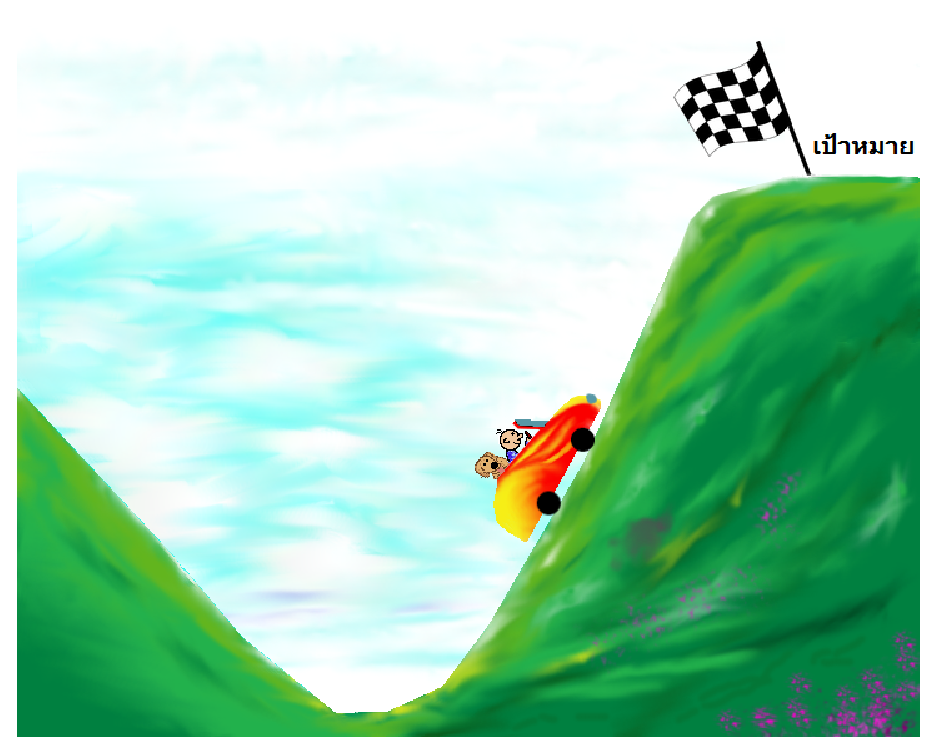
\includegraphics[width=\paperwidth]{mtncar.eps}}%
\maketitle
%}

%
\begin{figure}
\begin{center}
\includegraphics[width=5.5in]{mtnvalleyCar.png}
\end{center}
%\caption{mountain car}
%\label{fig: mtncar}
\end{figure}
%

\pagenumbering{gobble}
\clearpage
\pagenumbering{arabic}

\tableofcontents
\clearpage

\lstset{
    language=R,
    basicstyle=\ttfamily\small,
    breaklines=true,
    prebreak=\raisebox{0ex}[0ex][0ex]{\ensuremath{\hookleftarrow}},
    frame=lines,
    showtabs=false,
    showspaces=false,
    showstringspaces=false,
    keywordstyle=\color{blue},
    stringstyle=\color{green!50!black},
    commentstyle=\color{gray}\itshape,
    numbers=left,
    captionpos=t,
    escapeinside={(*}{*)}
}

\lstset{
    language=Matlab,
    basicstyle=\ttfamily\small,
    breaklines=true,
    prebreak=\raisebox{0ex}[0ex][0ex]{\ensuremath{\hookleftarrow}},
    frame=lines,
    showtabs=false,
    showspaces=false,
    showstringspaces=false,
    keywordstyle=\color{blue},
    stringstyle=\color{green!50!black},
    commentstyle=\color{gray}\itshape,
    numbers=left,
    captionpos=t,
    escapeinside={\%\{}{\%\}}
}

%\lstinputlisting[language=R, caption={Sigmoid}]{test.R}

%\begin{lstlisting}[language=R,caption={Hello World}]
%## test
%x$test <- v %*% q
%## ##* เวกเตอร์ (vector) $x = \vec{v} \cdot \vec{q}$.*)
%\end{lstlisting}

%\begin{proof}[ตัวอย่าง]
%Here is my important proof
%\end{proof}

%\begin{myexample}
%Here is my example.
%\end{myexample}

%\begin{myexample}[ตัวอย่างพิเศษ]
%Here is my example.
%\end{myexample}

\section*{สัญญลักษณ์}
\selectlanguage{thai}

ศาสตร์\textit{การเรียนรู้ของเครื่อง}อาศัยพื้นฐานทางคณิตศาสตร์ 
ดังนั้นเพื่อให้ลดความสับสนของตัวแปรคณิตศาสตร์ที่ใช้ 
สัญญลักษณ์ของตัวแปรคณิตศาสตร์จะใช้ตามแนวทางดังตารางข้างล่าง ยกเว้นแต่จะระบุเป็นอื่น
\\

\hspace{-0.5in}
\begin{tabular}{ |>{\arraybackslash}m{1.3in}  |>{\arraybackslash}m{1.3in} 
|>{\arraybackslash}m{1.4in} |>{\arraybackslash}m{1.4in}|}
%\begin{tabular}{|c|c|c|c|}
\hline 
ชนิดตัวแปร & แบบอักษร & ตัวอย่างอักษรลาติน & ตัวอย่างอักษรกรีก \\ 
\hline 
สเกล่าร์ & พิมพ์เล็กธรรมดา & $x$ & $\phi$ \\ 
\hline 
เวคเตอร์ & พิมพ์เล็กตัวหนา & $\mathbf{x}$ & $\bm{\phi}$ \\
\hline 
%เวคเตอร์ & พิมพ์เล็กตัวหนา & $\hm{x}$ & $\hm{\phi}$ \\
%\hline 
เมตริกซ์ & พิมพ์ใหญ่ตัวหนา & $\mathbf{X}$ & $\bm{\Phi}$ \\
\hline 
\end{tabular} 
\vspace{0.5cm}

ตัวอย่าง
เมตริกซ์ $\mathbf{X} \in \mathbb{R}^{2 \times 3}$ เช่น
\begin{eqnarray}
\mathbf{X} = \begin{bmatrix}
1.2 & 3.5 & -0.48 \\
0.63 & 0.0 & 123.0
\end{bmatrix}
\nonumber
\end{eqnarray}

เวคเตอร์ $\mathbf{x} \in \mathbb{R}^4$ เช่น
$\mathbf{x} = \begin{bmatrix}
10.0 & 0.75 & -44.6 & 1203.8
\end{bmatrix}^T
$\\
(หมายเหตุ ถ้าไม่ระบุเป็นอย่างอื่น เวคเตอร์จะหมายถึง\textit{เวคเตอร์แบบคอลัมน์})
\\
และ
สเกล่าร์ $x \in \mathbb{R}$ เช่น
$
x = 32.4
$
%สัญญลักษณ์อื่นๆใช้ หากไม่ได้ระบุ จะใช้ตามความนิยมทั่วไป เช่น $x^\ast$ หมายถึง ค่าตัวดีที่สุด เป็นต้น.

%
ตัวอักษรภาษาอังกฤษทั่วไปจะใช้รูปแบบ เช่น x, y, z.
รูปแบบสำหรับโปรแกรมคอมพิวเตอร์ ตัวแปรที่อ้างถึงตัวแปรจากโปรแกรมคอมพิวเตอร์ จะใช้รูปแบบ เช่น \verb|x, y, z| 
โดยตัวพิมพ์เล็กหรือตัวพิมพ์ใหญ่ขึ้นกับชื่อตัวแปรในโปรแกรม (ไม่เกี่ยวข้องกับโครงสร้างชนิดข้อมูลของตัวแปร) ดังนี้
\\
%ฟังชั่น \verb|rbf| นำไปปฎิบัติโดย \verb|rbf(x) = exp(-gamma*dist(x))|
%โปรแกรมคอมพิวเตอร์ จะเขียนอยู่ในรูปแบบ ดังนี้
%\vspace{0.5cm}
รูปแบบที่ 1
\begin{verbatim}
## Radial Basis Function
rbf <- function(x, gamma=0.1){
    return exp(-gamma*dist(x))
}
\end{verbatim}

\vspace{0.5cm}
%
หรือ รูปแบบที่ 2 (รูปแบบนี้ บางครั้งอาจแสดงเลขบรรทัดออกมาด้วย)
\begin{lstlisting}[language=R, numbers=none]
## Radial Basis Function
rbf <- function(x, gamma=0.1){
	exp(-gamma*dist(x))
}
\end{lstlisting}

%โดยใน รูปแบบที่ 2 บางครั้ง (ตามความเหมาะสม) อาจแสดงเลขบรรทัด หรือ อักขระตั้งระยะ (tab) ออกมาด้วย เช่น
%\begin{lstlisting}[language=R, showtabs=true]
%## Gram Matrix
%for i in np.arange(N):
%	for j in np.arange(N):
%		K[i,j] = rbf(x[:,i]) * rbf(x[:,j])
%## ##* รูปแบบนี้ อักขระตั้งระยะ (tab) จะแสดงออกมาให้เห็นชัดเจน *)
%\end{lstlisting}

%\lstinputlisting[language=R, caption={Sigmoid}]{test.R}

\pagebreak

\begin{shaded}
%``การสร้างงานศิลปะทุกอย่างทุกประเภท นอกจากจะต้องใช้ความฝึกหัดชัดเจนในทางปฏิบัติ ประกอบกับวิธีการที่ดีอย่างเหมาะสมแล้ว ศิลปินจำต้องมีความจริงใจและความบริสุทธิ์ใจในงานที่ทำด้วย จึงจะได้ผลงานที่มีค่าควรแก่การยอมรับนับถือ''\\
%พระราชดำรัสของ พระบาทสมเด็จพระเจ้าอยู่หัว\\
%(ในพิธีเปิดการแสดงศิลปกรรมแห่งชาติ ครั้งที่ 21 8 กันยายน 2515) 

%การจะพัฒนาทุกสิ่งทุกอย่างให้เจริญนั้นจะต้องสร้างและเสริมขึ้นจากพื้นฐานเดิมที่มีอยู่ก่อนทั้งสิ้น ถ้าพื้นฐานไม่ดีหรือคลอนแคลนบกพร่องแล้ว ที่จะเพิ่มเติมเสริมต่อให้เจริญขึ้นไปอีกนั้น ยากนักที่จะทำได้ จึงควรจะเข้าใจให้แจ้งชัดว่า นอกจากจะมุ่งสร้างความเจริญแล้ว ยังต้องพยายามรักษาพื้นฐานให้มั่นคง ไม่บกพร่อง พร้อมๆ กันไปด้วย 
%พระบรมราโชวาทของ พระบาทสมเด็จพระเจ้าอยู่หัว... (46)
%(ในพิธีพระราชทานปริญญาบัตรแก่นิสิตจุฬาลงกรณ์มหาวิทยาลัย ณ จุฬาฯ 10 ก.ค.2523) 

``หนังสือ เป็นเสมือนคลังที่รวบรวมเรื่องราว ความรู้ ความคิด วิทยาการทุกด้านทุกอย่าง ซึ่งมนุษย์ได้เรียนรู้ ได้คิดอ่าน และเพียรพยายามบันทึกภาษาไว้ด้วยลายลักษณ์อักษร หนังสือแพร่ไปถึงที่ใด ความรู้ความคิดก็แพร่ไปถึงที่นั่น หนังสือจึงเป็นสิ่งมีค่า และมีประโยชน์ที่จะประมาณมิได้ในแง่ที่เป็นบ่อเกิดการเรียนรู้ของมนุษย์'' \\
%\hspace{1.5in} 
---พระราชดำรัสของพระบาทสมเด็จพระเจ้าอยู่หัวรัชกาลที่เก้า
\end{shaded}

\vspace{-0.5in}
\section*{คำนำ}
%\nonumbering

หนังสือ\textit{การเรียนรู้ของเครื่องเบื้องต้น}เล่มนี้ 
อธิบายเนื้อหาที่เกี่ยวข้องกับวิทยาการ\textit{การเรียนรู้ของเครื่อง} โดยเฉพาะ\textit{โครงข่ายประสาทเทียม}.
โดยมีวัตถุประสงค์ที่จะนำเสนอ ภาพรวม พื้นฐาน การประยุกต์ใช้  การนำทฤษฏีซึ่งอธิบายด้วยสมการคณิตศาสตร์ไปเขียนโปรแกรม
รวมไปถึงการพัฒนาที่น่าสนใจ และแรงบันดาลใจที่เกี่ยวข้อง.
อย่างไรก็ตาม แม้จุดประสงค์หลักอย่างหนึ่งคือการนำเสนอภาพรวมของศาสตร์
แต่เนื่องจากความกว้างและลึก
รวมถึงความก้าวหน้าที่เติบโตอย่างต่อเนื่องและรวดเร็วของศาสตร์นี้
การจะครอบคลุมเนื้อหาทั้งหมดเป็นไปไม่ได้เลย.
ดังนั้นหนังสือเล่มนี้จัดทำเนื้อหาโดยยึดแนวคิดในการวางตัวเพียงเป็นจุดเริ่มต้น
ให้ผู้อ่านได้พอเข้าใจและเห็นคุณค่าของวิทยาการการเรียนรู้ของเครื่องและศาสตร์พื้นฐานเบื้องหลัง
% ฉันทะ วิริยะ จิตตะ วิมังสา
% และคุณค่าของการเรียนรู้ของเครื่อง  
%ผู้อ่านได้พอเห็นภาพ ได้ชื่นชมการพัฒนา ได้เข้าใจคุณค่าและประสิทธิผลการประยุกต์ใช้ และได้เห็นศักยภาพของศาสตร์นี้
รวมถึงการให้ผู้อ่านได้มีตัวอย่างโปรแกรมที่สามารถนำไปทดลองปฏิบัติได้ด้วยตนเอง
ไปจนถึงอภิปรายข้อสังเกตุและประเด็นที่สำคัญ นำเสนอเกร็ดความรู้ ให้แบบฝึกหัด %ที่หวังว่าจะช่วยให้ผู้อ่านที่สนใจได้เกิดความคิดเชิงวิเคราะห์ หรือสร้างแรงบันดาลใจข
และอำนวยความสะดวกในกรณีที่ผู้อ่านต้องการแหล่งค้นคว้าเพิ่มเติม. 
แนวคิดของลำดับเนื้อหาดังกล่าวข้างต้นนี้ ออกแบบมาเพื่อใช้ประกอบการเรียนการสอน วิชา\textit{โครงข่ายประสาทเทียม} วิชา\textit{การเรียนรู้ของเครื่อง} และวิชา\textit{การรู้จำรูปแบบและการตรวจจับภาพวัตถุ} ระดับปริญญาตรีและบัณฑิตศึกษา ของ% 
%ภาควิชาวิศวกรรมคอมพิวเตอร์ 
คณะวิศวกรรมศาสตร์ มหาวิทยาลัยขอนแก่น


% ซึ่งหวังว่าจะช่วยเสริมความเข้าใจของศาสตร์ได้ดียิ่งขึ้น %ไปจนถึง เกิดความคิด หรือ มีแรงบันดาลใจ ที่จะประยุกต์ใช้, พัฒนา, ปรับปรุง, หรือ ทำการศึกษาวิจัยในศาสตร์และศิลป์นี้ต่อไป.
%และ 
%ก็หวังว่า โดยอาศัยพื้นฐานบางส่วน จาก การเรียนรู้ของเครื่องเบื้องต้นเล่มนี้ 
%ทั้งหมดนี้ หากผู้อ่าน ที่ชื่นชอบและสนใจที่จะศึกษาเพิ่มเติม ก็จะสามารถทำได้สะดวกยิ่งขึ้น.

การเรียนรู้ของเครื่อง มีพื้นฐานมาจากหลากหลายศาสตร์ เช่น การหาค่าดีที่สุด ความน่าจะเป็น
หนังสือเริ่มด้วยการอธิบายภาพรวมของการเรียนรู้ของเครื่อง 
ตามด้วยการอธิบายศาสตร์พื้นฐานบางส่วน เพื่อให้ช่วยผู้อ่านสามารถทำความเข้าใจทฤษฎีเบื้องหลังได้ดียิ่งขึ้น 
แล้วจึงอธิบายวิธีการเรียนรู้ของเครื่องอย่างง่าย (โมเดลเชิงเส้น) 
ก่อนจะอธิบายวิธีโครงข่ายประสาทเทียม (ซึ่งเป็น หนึ่งในศาสตร์และศิลป์ของการเรียนรู้ของเครื่อง) 
ไปจนถึงการนำวิธีโครงข่ายประสาทเทียมไปประยุกต์ใช้งาน

%ผู้เขียนหวังว่า ตำราการประยุกต์ใช้การเรียนรู้ของเครื่องเล่มนี้ จะช่วยเป็นจุดเริ่มต้นให้ ผู้อ่านได้พอเห็นภาพ ได้ชื่นชมการพัฒนา ได้เข้าใจคุณค่าและประสิทธิผลการประยุกต์ใช้ และได้เห็นศักยภาพของศาสตร์นี้
%รวมถึง หากผู้อ่านได้ทดลองลงมือปฏิบัติ ก็จะช่วยเสริมความเข้าใจของศาสตร์ได้ดียิ่งขึ้น %ไปจนถึง เกิดความคิด หรือ มีแรงบันดาลใจ ที่จะประยุกต์ใช้, พัฒนา, ปรับปรุง, หรือ ทำการศึกษาวิจัยในศาสตร์และศิลป์นี้ต่อไป.
%และ 
%ก็หวังว่า โดยอาศัยพื้นฐานบางส่วน จาก การเรียนรู้ของเครื่องเบื้องต้นเล่มนี้ 
%หากผู้อ่าน ที่ชื่นชอบและสนใจที่จะศึกษาเพิ่มเติม ก็จะสามารถทำได้สะดวกยิ่งขึ้น.

\pagebreak

%\vfill
\begin{minipage}{6in}
{\small
\begin{shaded}
%หมายเหตุ 
เนื่องจากเนื้อหาของหนังสือเกี่ยวข้องกับคณิตศาสตร์และมี\textit{คำศัพท์เฉพาะ}จำนวนมาก 
รวมทั้งหนังสือเล่มนี้จัดเตรียมด้วยโปรแกรมเลเท็กซ์. 
ดังนั้น เพื่อช่วยให้เนื้อหาอ่านง่ายขึ้น และเพื่อช่วยการตัดประโยคของเลเท็กซ์ รูปแบบการเขียนอาจจะมีการเว้นวรรคตอนมากกว่างานเขียนภาษาไทยโดยทั่วไป 
และเพื่อลดความสับสนจากวรรคตอน ผู้เขียนใช้\textit{มหัพภาค}เพื่อช่วยบอกการจบประโยค
รวมถึงบางครั้งผู้เขียนใช้\textit{ฟอนต์ตัวเอียง}เพื่อเน้นคำศัพท์หรือกลุ่มคำให้ชัดเจนขึ้น
ตัวอย่างเช่น ``วิธีที่ดีที่สุดในการเรียนรู้\textit{ศาสตร์การเรียนรู้ของเครื่อง}ก็คือการลองลงมือทำ.''
ทั้งนี้ผู้เขียนต้องขออภัยสำหรับประเด็นดังกล่าวด้วย.

การเรียบเรียงจัดทำเนื้อหาของการเรียนรู้ของเครื่องเบื้องต้นเล่มนี้  ได้รับอิทธิพลหลักจากตำราการรู้จำรูปแบบและการเรียนรู้ของเครื่อง\cite{Bishop2006a} และ วิดีทัศน์สอนวิชาการเรียนรู้ของเครื่อง\cite{Ng2013a}
โดยอาจมีแหล่งอื่นๆเพิ่มเติมอีกตามเนื้อหาเฉพาะ เช่น \textit{การหาค่าดีที่สุด}ได้รับอิทธิพลหลักจากตำราการหาค่าดีที่สุดเบื้องต้น\cite{ChongZak2ndEd}.
\end{shaded}
}
\end{minipage}


%คอมไพล์ด้วย
%\begin{verbatim}
%xelatex mlbook.tex
%xelatex mlbook.tex
%bibtex mlbook
%makeindex mlbook
%xelatex mlbook.tex
%xelatex mlbook.tex
%\end{verbatim}




%%%%%%%%%%%%%%%%%%%%%%%%%%%%%%%%%%%%%%%%%%%%%%%%%%%%%%%%%%%%%%%%%%%

%% introduction Andrew Ng's Lecture 1 & Bishop Chapter 1
\chapter{บทนำ}
\label{chapter: introduction}

\begin{verse}
``Adapt or perish, now as ever, is nature's inexorable imperative.'' \\
---H.~G.~Wells 
\end{verse}

\begin{verse}
``ปรับตัว หรือ สูญพันธุ์ เป็นความจำเป็นของธรรมชาติที่ไม่อาจหลีกเลี่ยงได้ ทั้งตอนนี้เฉกเช่นตลอดมา'' 
---เอช จี เวลส์ \\
\end{verse}

วิธี\textit{การเรียนรู้ของเครื่อง}ถูกประยุกต์ใช้อย่างกว้างขวางในวงการธุรกิจ อุตสาหกรรม การทหาร วงการวิทยาศาสตร์ บันเทิง รวมถึงการประยุกต์ใช้ชีวิตประจำวัน
ตัวอย่างเช่น 
ลักษณะงานที่เป็น\textit{การทำเหมืองข้อมูล} การตรวจสอบหารูปแบบการใช้บัตรเครดิตที่ผิดปกติ\cite{DeviEtAl2014a} ซึ่งอาจเนื่องมาจากการที่บัตรถูกขโมยไป
การบริหารการลงทุนทางการเงิน\cite{TanEtAl2011a}
งานแอพพลิเคชั่นที่ไม่สามารถโปรแกรมตรงๆได้ (หรือ ทำได้ยากมาก) เช่น ระบบอ่านลายมือเขียน\cite{LeCunEtAl1990a}
การควบคุมเฮลิคอปเตอร์ไร้นักบิน\cite{CoatesEtAl2009a} 
การควบคุมหุ่นยนต์ที่มีการเครื่องไหวที่ซับซ้อน\cite{AkiyamaEtAl2010a}
การบริหารจัดการทรัพยกรนำ้\cite{CastellettiEtAl2013a}
การปรับตั้งค่าของเวอร์ชัวร์แมชชีน\cite{RaoEtAl2009a}
การพัฒนารถยนต์ที่ขับเคลื่อนได้เองโดยไร้คนขับ\cite{ZhuEtAl2014a}
การติดตามลักษณะโครงสร้างใต้น้ำอัตโนมัติ\cite{MagazzeniEtAl2014a}
การระบุหารังสีแกมม่าจากข้อมูลกล้องโทรทัศน์\cite{BockEtAl2004a}
ระบบตรวจสอบการสั่นสะเทือนของแผ่นดินไหว\cite{RuanoEtAl2014a}
การหารูปแบบในข้อมูลชีวสารสนเทศ\cite{KelchtermansEtAl2014a}
การแปลภาษาอัตโนมัติ\cite{CostaFarrus2014a}
ระบบรู้จำคำพูด\cite{SarikayaEtAl2014a}
ระบบรู้จำความก้าวหน้าของคอร์ดดนตรี\cite{YuElAl2013a}
ใช้กับงานศิลปะ\cite{CuljakEtAl2011a}
กีฬา\cite{HolstJanasson2013a}
ระบบรู้จำใบหน้า\cite{BarnardEtAl2013a}
ระบบตรวจสอบความผิดปกติของสัญญาณคลื่นไฟฟ้าหัวใจ\cite{LiEtAl2012a}
การแยกอีเมล์ที่เป็นสแปม\cite{BlanzieriBryl2008a} 
ระบบแนะนำหนังสือ เพลง วิดีโอ หรือสินค้า\cite{GhazanfarPrugel-Bennett2014a}
การจำแนกหรือระบุหัวข้อสำหรับข้อความ\cite{BleiEtAl2003a}
หรือ แม้แต่เพิ่มประสิทธิภาพของงานของระบบควบคุม ระบบตัดสินใจ ที่ซับซ้อน ระบบควบคุมการระบายอากาศ-เครื่องทำความร้อน--เครื่องปรับอากาศ\cite{AndersonEtAl2004a} 
ระบบควบคุมสินค้าคงคลัง\cite{KatanyukulEtAl2011a, KatanyukulEtAl2012a, Katanyukul2013a, KatanyukulChong2014a} 
ระบบควบคุมการจราจร\cite{ChanlohaEtAl2014a} เป็นต้น 

%\begin{minipage}{5.5in}
{\small
\begin{shaded}
%Data mining, also called knowledge discovery in databases, in computer science, the process of discovering interesting and useful patterns and relationships in large volumes of data. The field combines tools from statistics and artificial intelligence (such as neural networks and machine learning) with database management to analyze large digital collections, known as data sets. Data mining is widely used in business (insurance, banking, retail), science research (astronomy, medicine), and government security (detection of criminals and terrorists).
%
การทำเหมืองข้อมูล (Data Mining) หรือ บางครั้งเรียกว่า การค้นหาความรู้ในฐานข้อมูล (Knowledge Discovery in Databases) หมายถึง กระบวนการค้นหารูปแบบหรือความสัมพันธ์ที่น่าสนใจและมีประโยชน์ในข้อมูลขนาดใหญ่
{\footnotesize (จาก Encyclopedia Britainica \verb|https://global.britannica.com/technology/data-mining| สืบค้น 9 สิงหาคม 2559)}
%
การทำเหมืองข้อมูล เน้นที่การค้นหารูปแบบที่น่าสนใจ 
ซึ่งแม้การทำเหมืองข้อมูลอาจจะใช้เทคนิคที่จัดเป็นวิธีการเรียนรู้ของเครื่อง เช่น การหากฏความสัมพันธ์ (Association Rules) การแบ่งกลุ่มข้อมูล (Cluster Analysis) การจำแนกข้อมูล (Classification) เป็นต้น.
แต่ในทางปฏิบัติ บ่อยครั้งที่ในกระบวนการที่สมบูรณ์ของการทำเหมืองข้อมูลจะต้องอาศัยการทำงานของมนุษย์ เช่น กระบวนการอาจมีการใช้มนุษย์ เพื่อตรวจสอบกลั้นกรองผลลัพธ์ที่ได้จากวิธีการเรียนรู้ของเครื่อง
%ความสัมพันธ์ที่น่าสนใจและมีประโยชน์ จากกฏความสัมพันธ์ที่ค้นพบทั้งหมดโดยการหากฏความสัมพันธ์ด้วยคอมพิวเตอร์
หรือแม้แต่กระบวนการการทำเหมืองข้อมูล อาจใช้เพียงการทำงานของมนุษย์ โดยเขียนภาษาสอบถามจากฐานข้อมูล เพื่อค้นหารูปแบบที่น่าสนใจ โดยไม่ต้องอาศัยวิธีของการเรียนรู้ของเครื่องเลยก็ได้.
%
ในขณะที่มุมมองทั่วไปคือการทำเหมืองข้อมูลใช้วิธีจากการเรียนรู้ของเครื่อง 
การเรียนรู้ของเครื่องเองก็อาจจะถูกสร้างขึ้นได้ 
โดยอาศัยข้อมูลและรูปแบบที่ถูกค้นพบโดยการทำเหมือนข้อมูลได้เช่นกัน
\end{shaded}
}
%\end{minipage}


การเรียนรู้ของเครื่อง (Machine Learning) จัดเป็นศาสตร์แขนงหนึ่งของ\textit{ปัญญาประดิษฐ์}. 
ความสำเร็จที่สำคัญๆในวงการปัญญาประดิษฐ์หลายๆอย่าง ก็อาศัยศาสตร์การเรียนรู้ของเครื่อง เช่น โปรแกรมเล่นเกมส์แบคแกมมอน\cite{TDGammon} และ โปรแกรมเล่นหมากล้อม\cite{SilverEtAl2016a} ที่สามารถเล่นได้ระดับสูงสุดเมื่อเทียบกับมนุษย์ 
หรือ ไอบีเอ็มวัตสันที่สามารถชนะมนุษย์ได้ในเกมส์ตอบคำถามเจ๊บพาดี้\cite{Abu-Mostafa2012a}.
%
ประสิทธิผลของการเรียนรู้ของเครื่องและศักยภาพของศาสตร์นี้ทำให้มีการศึกษาวิจัยอย่างกว้างขวางและกระตือรือร้น.
ศาสตร์และศิลป์ของการเรียนรู้ของเครื่อง จึงมีการพัฒนาอย่างมีนัยสำคัญอย่างต่อเนื่อง. 
%
ดาร์พาหรือองค์การโครงการวิจัยชั้นสูงทางการป้องกันประเทศของสหรัฐอเมริกา
(Defense Advanced Research Projects Agency) 
ซึ่งอยู่เบื้องหลังเทคโนโลยีหลายอย่างที่มีผลกระทบต่อเศรษฐกิจและสังคมของทั่วโลก เช่น เทคโนโลยีอินเตอร์เนต 
ก็ให้ความสำคัญและสนับสนุนการวิจัยและพัฒนาศาสตร์และศิลป์ของเทคโนโลยีการเรียนรู้ของเครื่องอย่างกว้างขวาง 
ดังสะท้อนออกมาจากวิสัยทัศน์ของเคทเธอลีนฟิชเชอร์
% (Kathleen Fisher) แห่งดาร์พา 
ที่กล่าวผ่านเวปไซตของดาร์พา ที่ลงข่าวเมื่อ 19 มี.ค. พ.ศ. 2556 ว่า 
%“Our goal is that future machine learning projects won’t require people to know everything about both the domain of interest and machine learning to build useful machine learning applications. Through new probabilistic programming languages specifically tailored to probabilistic inference, we hope to decisively reduce the current barriers to machine learning and foster a boom in innovation, productivity and effectiveness.”
เป้าหมายของดาร์พาคือโครงการ\textit{การเรียนรู้ของเครื่อง}ในอนาคต ที่สามารถสร้างโปรแกรม\textit{การเรียนรู้ของเครื่อง}ที่มีประโยชน์ได้เอง โดยที่ไม่จำเป็นต้องมีมนุษย์ช่วยในกระบวนการเรียนรู้ ไม่ว่าจะเพื่อความชำนาญเฉพาะเรื่อง หรือ เพื่อการสร้างโปรแกรมการเรียนรู้ของเครื่อง% 
\footnote{ข้อมูลจาก \texttt{http://www.darpa.mil/NewsEvents/Releases/2013/03/19a.aspx}, สืบค้น 5 ก.ย. 2556}
%

%\begin{minipage}{5.5in}
{\small
\begin{shaded}
ปัญญาประดิษฐ์ (Artificial Intelligence คำย่อ AI)
เป็นศาสตร์ของการออกแบบโปรแกรมคอมพิวเตอร์ที่มีเหตุมีผลเพื่อภารกิจเป้าหมาย
โดยที่โปรแกรมนั้นจะเลือกการกระทำที่ช่วยให้ภารกิจมีโอกาสสำเร็จมากที่สุด 
บนพื้นฐานของสถานะการณ์ที่รับรู้และความรู้เดิมที่ใส่ไว้
แม้จะมีความไม่แน่นอนเกี่ยวข้องอยู่
%
%"For each possible precept sequence, 
%a rational agent should select an action that is expected to 
%maximize its performance measure, given the evidence provided by
%the percept sequence and whatver built-in knowledge the agent has."

นอร์วิคและรัสเซล\cite{RussellNorvig2009a}ได้ยกตัวอย่างศาสตร์ต่างๆที่
%ต้องการ สำหรับการพัฒนาระบบคอมพิวเตอร์ที่จะสามารถทำตัวได้เหมือนมนุษย์ และ
%ศาสตร์เหล่านี้ต่างก็
จัดอยู่ภายใต้ความหมายของปัญญาประดิษฐ์ ได้แก่
ศาสตร์การประมวลผลภาษาธรรมชาติ (Natural Language Processing) %สำหรับการสื่อสารกับมนุษย์ ในภาษาของมนุษย์ (ไม่ใช่ภาษาโปรแกรมคอมพิวเตอร์),
ศาสตร์การแทนความรู้ (Knowledge Representation) %สำหรับการเก็บสิ่งที่ได้รับรู้มา,
ศาสตร์คอมพิวเตอร์วิทัศน์ (Computer Vision)
ศาสตร์วิทยาการหุ่นยนต์ (Robotics)
และ
ศาสตร์การเรียนรู้ของเครื่อง เป็นต้น.
%สำหรับการปรับตัวเข้ากับสถานะการณ์ และความสามารถในการขยายความสามารถของตัวเองเกินกว่าที่ผู้ออกแบบได้กำหนดไว้,
%
นอกจากศาสตร์ดังกล่าวข้างต้นนี้ ศาสตร์ปัญญาประดิษฐ์ก็ยังเกี่ยวข้องสัมพันธ์กับตรรกศาสตร์ ศาสาตร์การหาค่าดีที่สุด  วิศวกรรมความรู้ ศาสตร์การจัดการความไม่แน่นอนซึ่งรวมถึงสถิติศาสตร์ เป็นอย่างมาก ดังเห็นได้จากคำนิยามของปัญญาประดิษฐ์เอง
\end{shaded}
}
%\end{minipage}


\section{การเรียนรู้ของเครื่องคืออะไร}
\index{Machine Learning}
\index{การเรียนรู้ของเครื่อง}

ในปี ค.ศ. 1959 อาร์เธอร์ ซามูเอล %(Arthur Samuel) 
เขียนโปรแกรม ให้คอมพิวเตอร์เล่นหมากฮอร์ส\cite{SamuelML} 
%(Checker playing program) 
แต่ซามูเอลเองเล่นหมากฮอร์สไม่เก่งเลย.
ดังนั้นแทนที่ซามูเอลจะโปรแกรมสั่งคอมพิวเตอร์ว่าควรจะเดินหมากอย่างไร
แต่ซามูเอลกลับโปรแกรมให้คอมพิวเตอร์เล่นแข่งกันเอง และโปรแกรมให้คอมพิวเตอร์เก็บผลว่า
ตำแหน่งของหมากอย่างไรที่เป็นตำแหน่งที่ดี ซึ่งนำไปสู่ชัยชนะ 
หรือตำแหน่งไหนเป็นตำแหน่งไม่ดี และมักจะทำให้แพ้ 
แล้วให้โปรแกรมเลือกเดินหมากตามผลที่เก็บนั้น.
หลังจากซามูเอลให้โปรแกรมเล่นแข่งกันเองหลายหมื่นกระดาน โปรแกรมเล่นหมากฮอร์สของซามูเอลก็สามารถเล่นหมากฮอร์สได้ดีมาก 
และเล่นได้ดีกว่าตัวของซามูเอลเอง.
ณ ตอนนั้น วิธีการสร้างโปรแกรมเล่นหมากฮอร์สของซามูเอลเป็นแนวทางใหม่มาก 
และก็ให้ผลลัพธ์ที่ดีอย่างมาก ซึ่งได้เปิดเผยถึงศักยภาพของแนวคิดนี้

อาร์เธอร์ ซามูเอล ได้นิยามการเรียนรู้ของเครื่อง ไว้ว่า 
%``Field of study that gives computers the ability to learn without being explicitly programmed.''\cite{SamuelML}
%สรุปใจความได้ว่า 
%\begin{verse}
การเรียนรู้ของเครื่องคือการทำให้คอมพิวเตอร์มีความสามารถที่จะเรียนรู้ได้ โดยที่ไม่ต้องเขียนโปรแกรมวิธีทำตรงๆ.
%\end{verse}
%
ทอม มิทเชล นักวิจัยชั้นนำทางด้านการเรียนรู้ของเครื่อง 
ช่วยขยายความโดยการให้นิยามไว้ว่า
%การเรียนรู้ของเครื่อง คือ 
%\begin{verse}
โปรแกรมคอมพิวเตอร์จะเรียกได้ว่า มีการเรียนรู้จากประสบการณ์ $E$ ซึ่งเกี่ยวข้องกับภารกิจ $T$ และสมรรถนะ $P$
ก็ต่อเมื่อสมรรถนะของการทำภารกิจ $T$ ที่วัดด้วย $P$ ปรับปรุงขึ้นได้จากประสบการณ์ $E$
\cite{Mitchell1997a}
%\end{verse}
%\begin{verse}
%``''
%``Well-posed Learning Problem: A computer program is said to learn from experience E with respect to some task T and some performance measure P, if its performance on T, as measured by P, improves with experience E.''\cite{Mitchell1997a} \\
%\end{verse}

คำนิยามนี้ค่อนข้างจะเป็นทางการและมีนัยทางรูปธรรมอยู่มาก.
%สรุปใจความได้ว่า การเรียนรู้ของเครื่อง คือ โปรแกรมคอมพิวเตอร์ ที่เรียนรู้จากประสบการณ์ $E$ เพื่อจะทำงาน $T$ ที่มีตัววัดผลการทำงาน $P$ และ สามารถทำให้ผลการทำงาน $T$ ที่วัดด้วย $P$ ดีขึ้นได้จากประสบการณ์ที่ได้จาก $E$.
%
จากตัวอย่าง โปรแกรมเล่นหมากฮอร์สของซามูเอล 
ประสบการณ์ $E$ คือการเดินหมากและผลที่โปรแกรมเล่นแข่งกันเอง
ภารกิจ $T$ คือการเล่นหมากฮอร์ส
และสมรรถนะ $P$ คือความน่าจะเป็นที่โปรแกรมจะเล่นชนะ

ตัวอย่างที่สอง โปรแกรมเลือกหัวข้อสำหรับข้อความ\cite{BleiEtAl2003a} 
ประสบการณ์ $E$ คือการลองเลือกคำในข้อความไปเปรียบเทียบกับเนื้อหาในข้อความอื่นๆ
ภารกิจ $T$ คือการเลือกคำในข้อความมาเป็นหัวข้อ
และสมรรถนะ $P$ คือความน่าจะเป็นที่คำที่เลือกมาจะเป็นตัวแทนเนื้อหาของข้อความ

%โปรแกรมกรองอีเมล์ขยะ % (spam email filtering) 
%ที่เวลา เราเข้าไปใช้อีเมล์ แล้ว เราอาจจะคลิก ``spam'' เพื่อแจ้งโปรแกรมว่าอีเมลล์ที่เราได้เป็นอีเมล์ขยะ และ โปรแกรมสามารถ เรียนรู้ จากการรายงานของเรา เพื่อที่จะกรองอีเมล์ได้ดีขึ้น.
%ประสบการณ์ $E$ คือ โปรแกรม ดู การคลิกรายงานอีเมล์ขยะของเรา.
%งาน $T$ คือ การจำแนกแยกอีเมล์ ว่าเป็นอีเมล์ขยะ หรือ อีเมล์ไม่ใช่ขยะ.
%ตัววัดการทำงาน $P$ คือ อัตราส่วน จำนวนอีเมล์ที่ถูกแยกได้อย่างถูกต้อง ต่อ จำนวนอีเมล์ทั้งหมด

ตัวอย่างที่สาม โปรแกรมรู้จำลายมือแยกตัวเลข เช่น การแยกแยะรูปลายมือเขียนของตัวเลขต่างๆ ดังแสดงในรูปที่~\ref{fig: example ZIP image digits}. 
นั่นคือ การแยกแยะออกมาว่า แต่ละรูปภาพเป็นรูปภาพของตัวเลขอะไร. 
ประสบการณ์ $E$ คือการดูตัวอย่างรูปภาพตัวเลขที่เป็นลายมือเขียนและเฉลยตัวเลขที่อ่านออกมา.
ภารกิจ $T$ คือการจำแนกแยกรูปภาพลายมือเขียน ว่าเป็นรูปภาพของเลขอะไรระหว่าง $0$ ถึง $9$.
และสมรรถนะ $P$ คืออัตราส่วน\textit{จำนวนรูปภาพที่ถูกจำแนกได้ถูกต้อง}ต่อจำนวนรูปภาพทั้งหมด.

%
\begin{figure}
\begin{center}
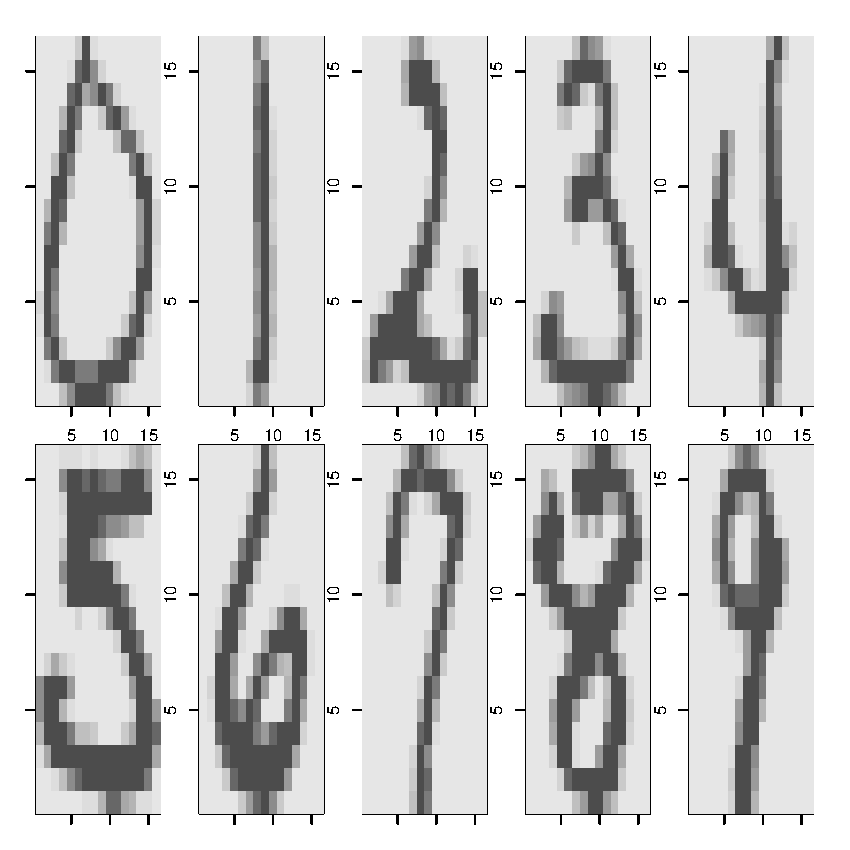
\includegraphics[width=2.0in]
{01Intro/zipdigits.eps}
\end{center}
\caption{ตัวอย่างรูปตัวเลขจากลายมือเขียน}
\label{fig: example ZIP image digits}
\end{figure}
%

%หัวข้อชี้แจง ภาพรวมของการเรียนรู้ของเครื่อง.
%ตลอดตำราเล่มนี้ ผู้เขียนใช้ ฟอนต์เข้ม เช่น $\mathbf{x}$ เพื่อระบุถึงตัวแปรที่เป็นเวกเตอร์ หรือ เมตริกซ์, เพื่อเตือนให้ผู้อ่านนึกภาพตามได้ถูกต้อง เปรียบเทียบกับตัวแปรค่าเดี่ยว เช่น $x$.
%และให้ฟอนต์ \verb|sigmoid| เพื่อแสดงโค้ด ซึ่งต่างจาก $\mathbf{sigmoid}$ ที่แสดงถึงฟังชั่นทางคณิตศาสตร์.

\section{ภาพรวมของการเรียนรู้ของเครื่อง}
\label{sec: ML overview}

\paragraph{ตัวอย่างการรู้จำลายมือแยกตัวเลข.}

รูปที่~\ref{fig: example ZIP image digits} แสดงตัวอย่างรูปภาพที่ต้องการโปรแกรมรู้จำลายมือ เพื่อแยกรูปออกตามตัวเลขที่ภาพแสดง โดยมีรูปภาพของตัวเลขตั้งแต่ $0$ ถึง $9$.
รูปภาพแต่ละรูปเป็น\textit{ภาพขาวดำ} (grayscale) มีขนาด $16 \times 16$ พิกเซล (pixels) 
และ\textit{ค่าของแต่ละพิกเซล}แทนด้วยเลขจำนวนจริง.
ดังนั้น รูปหนึ่งรูปสามารถแทนได้ด้วยตัวแปรเวกเตอร์ของจำนวนจริงขนาด $256$ ($=16 \times 16$) 
หรือคือสามารถกำหนด $\mathbf{x} \in \mathbb{R}^{256}$ แทนรูปหนึ่งรูป.
ในทางปฏิบัติ เราไม่สามารถเขียนโปรแกรมนี้จากกฎตายตัวได้ 
หรือถ้าได้ก็อาจจะได้ผลการทำงานที่แย่มากหรือทำได้ยากมากๆ.

แต่\textit{โปรแกรมรู้จำลายมือแยกตัวเลข}สามารถเขียนขึ้นได้อย่างมีประสิทธิภาพด้วยแนวทางของศาสตร์การเรียนรู้ของเครื่อง.
จุดประสงค์ที่ต้องการคือโปรแกรมที่จะบอกได้ว่า\textit{รูปภาพเป็นรูปภาพของเลขใด} 
หรือกล่าวอีกอย่างคือ การทายฉลาก $y \in \{0, 1, 2, \ldots, 9\}$ ที่เหมาะสม จากรูปภาพ $\mathbf{x}$.

แนวทางของการเรียนรู้ของเครื่องคือจะใช้โมเดลทางคณิตศาสตร์ในการหาค่าเอาท์พุต $y$ จาก อินพุต $\mathbf{x}$ โดย ตัวโมเดลจะถูกควบคุมด้วยพารามิเตอร์ $\bm{\theta}$.
โมเดล $f:\mathbf{x},\bm{\theta} \mapsto y$ อาจเขียนได้เป็น $y = f(\mathbf{x}|\bm{\theta})$ โดย 
$y$ คือ\textit{เอาท์พุต} (หรืออาจจะเรียก\textit{คำตอบ}หรือ\textit{ฉลากของกลุ่ม})
และ $\mathbf{x}$ คือ\textit{อินพุต} หรือเวกเตอร์ค่าของพิกเซล
และ $\bm{\theta}$ คือ\textit{พารามิเตอร์}%
ที่จะสามารถปรับพฤติกรรมการทำงานของโมเดลให้เป็นไปในทางที่ต้องการได้.

โมเดลทางคณิตศาสตร์นี้  
ในทางทฤษฎีแล้ว 
บางโมเดลมีความยืดหยุ่นสูงมาก (เช่น โมเดลโครงข่ายประสาทเทียม) จะสามารถปรับตัวเป็นฟังชั่นอะไรก็ได้ ขึ้นกับการปรับค่าพารามิเตอร์ $\bm{\theta}$.
%
ในการปรับหาค่าพารามิเตอร์ $\bm{\theta}$ ที่เหมาะสม ผู้สร้างโมเดลจะใช้ตัวอย่างของรูปภาพตัวเลข $N$ ภาพ แทนด้วยตัวแปร $\mathbf{X} = [\mathbf{x}_1, \ldots, \mathbf{x}_N]$ พร้อมฉลากเฉลย $N$ ฉลาก แทนด้วยตัวแปรเมตริกซ์ขนาด $1 \times N$ นั่นคือ $\mathbf{T} =[t_1, \ldots, t_N]$.
ฉลากเฉลยนี้อาจได้มาจากการใช้ให้คนดูรูปภาพและระบุฉลากที่ถูกต้องของแต่ละภาพไว้.
ข้อมูล $\mathbf{X}$ และ $\mathbf{T}$ นี้จะถูกเรียกว่า ``ข้อมูลชุดฝึกหัด'' (training dataset).

%นอกจาก รูปภาพตัวเลข $N$ ภาพ: $\mathbf{x}_1, \ldots, \mathbf{x}_N$ แล้ว, ข้อมูลในชุดฝึกหัดนี้ จะมี เฉลย หรือ ตัวอย่างคำตอบ หรือ ฉลากบอกกลุ่มของรูปภาพตัวเลข $t_1, \ldots, t_N$ มาด้วย.
%กล่าวโดยย่อ เราจะมี ตัวอย่างรูป $\mathbf{x}$ และ ตัวอย่างคำตอบ $\mathbf{t}$ เพื่อใช้ในการปรับหาค่าพารามิเตอร์ $\theta$.

อัลกอริทึ่ม\textit{การเรียนรู้ของเครื่อง}จะช่วยหาค่าที่เหมาะสมของพารามิเตอร์ $\bm{\theta}^*$ ออกมา.
ขั้นตอนในการใช้ข้อมูลชุดฝึกหัดเพื่อปรับหาค่าพารามิเตอร์จะเรียกว่า \textit{การฝึกหัด} (training) 
หรือ\textit{การเรียนรู้} (learning).
ผลลัพธ์ที่ได้จาก\textit{การเรียนรู้}คือโมเดลที่พร้อมใช้งาน $f^*(\mathbf{x}) = f(\mathbf{x}|\bm{\theta}^*)$ ที่สามารถใช้ทายค่าฉลากของรูปภาพได้.
นั่นคือ สำหรับรูปภาพ $\mathbf{x}'$ โมเดลจะทายฉลาก $y' = f^*(\mathbf{x}')$.

\paragraph{การประเมินผล.} 
โมเดลที่ดีจะต้องสามารถทายค่าฉลากของรูปภาพใหม่ได้ดี.
รูปภาพใหม่ที่กล่าวถึงนี้ คือรูปภาพที่ไม่ได้ถูกใช้ในขั้นตอนการฝึกโมเดล.
การประเมินผลการทำงานของโมเดลจะใช้ข้อมูลอีกชุด 
โดยที่ข้อมูลชุดนี้จะต้องไม่ได้ถูกใช้ในการฝึกหัด.
ข้อมูลชุดนี้เรียกว่า ``ข้อมูลชุดทดสอบ'' (test dataset).
ความสามารถที่โมเดลทายหรือระบุฉลากของข้อมูลใหม่ได้ดี เรียกว่า \textit{คุณสมบัติความทั่วไป} 
หรือ\textit{คุณสมบัติเจนเนอรอลไลเซชั่น} (Generalization).
เราต้องการโมเดลที่มี\textit{คุณสมบัติความทั่วไป}ที่ดี.
นั่นคือ โมเดลสามารถระบุฉลากได้ถูกต้อง แม้ว่ารูปภาพนั้นจะเป็นรูปใหม่ที่ไม่เคยเห็นมาก่อน.
%
จากตัวอย่างการรู้จำลายมือแยกตัวเลขข้างต้น แม้จะเป็นตัวอย่างง่ายๆ
แต่ภาพรวมและหลักการที่สำคัญหลายๆอย่างที่อภิปรายไปนั้น 
ก็ครอบคลุมแนวทางของการเรียนรู้ของเครื่องโดยทั่วๆไป.

หัวข้อ~\ref{section: Polynomial Curve Fitting} จะอภิปรายฟังชั่นโพลิโนเมียล ที่เป็นโมเดลที่มีรูปแบบทางคณิตศาสตร์ที่ไม่ซับซ้อน %กับ งานการหาค่าถดถอยมิติเดียว, 
ซึ่งน่าจะช่วยให้ผู้อ่านเข้าใจแนวคิดและภาพรวมของการสร้างโมเดลและการปรับหาค่าพารามิเตอร์ได้ดียิ่งขึ้น.
%
บทที่~\ref{chapter: ANN} จะอภิปรายถึงโครงข่ายประสาทเทียม ซึ่งเป็นโมเดลที่มีความซับซ้อนมาก และจัดเป็นหนึ่งในศาสตร์และศิลป์ของวิชาการเรียนรู้ของเครื่อง.
บทที่~\ref{chapter: Applications of ANN} จะสาธิตการประยุกต์ใช้งานโครงข่ายประสาทเทียม
รวมถึงตัวอย่างงานการรู้จำลายมือแยกตัวเลขนี้ เพื่อให้ผู้อ่านได้เห็นภาพโดยสมบูรณ์.

\paragraph{การเตรียมและปรับข้อมูลก่อนและหลัง.} 
ในทางปฏิบัติแล้ว ส่วนใหญ่ อินพุต $\mathbf{x}$ มักจะถูกเตรียมหรือปรับปรุงเบื้องต้นก่อน 
เพื่อเปลี่ยนไปอยู่ในปริภูมิของตัวแปร
(Space of Variables) 
ที่โมเดลจะสามารถทำงานได้ง่ายขึ้น.
ตัวอย่างเช่น อินพุตของโปรแกรมรู้จำลายมือแยกตัวเลข อาจจะถูกปรับให้ ขนาดภาพของตัวเลขแต่ละตัวมีความสูงและความกว้างพอๆกันก่อน 
ซึ่งจะช่วยทำให้สร้างโมเดลเพื่อแยกตัวเลขได้ง่ายขึ้น.
ขั้นตอนในการเตรียมข้อมูลเบื้องต้นนี้ (pre-processing) บางครั้งจะรวมขั้นตอนที่เรียกว่า ``การแยกลักษณะสำคัญ'' (feature extraction) เข้าไปด้วย (ดู~\cite{KatanyukulPonsawat2016a} สำหรับคำอธิบาย และตัวอย่างการแยกลักษณะสำคัญ).
ในบางกรณีการปรับข้อมูลภายหลัง (post-processing) ก็อาจถูกมานำใช้ เพื่อเพิ่มหรือปรับปรุงคุณภาพของเอาท์พุตจากโมเดลได้ เช่น การถอดรหัสแบบหนึ่งไปเค
(1-to-K decoder)
เพื่อปรับเอาต์พุตจากโมเดลจำแนกกลุ่มให้อยู่ในรูปแบบที่ต้องการ (ดูหัวข้อ~\ref{section: multiclass classification} สำหรับรายละเอียด)

\paragraph{ประเภทของการเรียนรู้ของเครื่อง.} 
หากมองจากมุมของประสบการณ์ $E$ ที่คอมพิวเตอร์ใช้ปรับปรุงการทำงาน โปรแกรมรู้จำลายมือแยกตัวเลขต้องการประสบการณ์ ซึ่งคือตัวอย่างอินพุต $\mathbf{X}$ และตัวอย่างเอาท์พุต $\mathbf{T}$.
การเรียนรู้ของเครื่องที่เกี่ยวข้องกับประสบการณ์เช่นนี้ จะเรียกว่า ``การเรียนรู้แบบมีผู้ช่วยสอน'' (Supervised Learning).
\index{Supervised Learning}
\index{การเรียนรู้แบบมีผู้ช่วยสอน}
เมื่อมองจากลักษณะของเอาท์พุต ปัญหาการรู้จำลายมือแยกตัวเลขมีเอาท์พุตเป็นฉลากของกลุ่ม ซึ่งจำนวนกลุ่มมีจำนวนแน่นอน เช่น $10$ กลุ่ม ตั้งแต่ `0' ถึง `9'.
\textit{ปัญหาแบบนี้}จัดเป็นชนิดปัญหาของ\textit{การจำแนกประเภท} (Classification).
แต่หากเอาท์พุตมีลักษณะเป็นเลขจำนวนจริง เช่น การทำนายปริมาณน้ำฝน การทำนายปริมาณแร่ธาตุในดิน การทำนายปริมาณน้ำยางจากต้นยางที่ปลูกในสภาพต่างๆ การทำนายแรงที่เกิดกับใบพัดลักษณะต่างๆของกังหันลม การทำนายมูลค่าการซื้อขายหลักทรัพย์
ปัญหาในลักษณะแบบนี้จะจัดเป็นชนิดปัญหาของ\textit{การหาค่าถดถอย} (Regression).
บทที่~\ref{chapter: Linear Models}~และ~\ref{chapter: ANN} จะอภิปรายถึงการเรียนรู้แบบมีผู้ช่วยสอน ทั้งสองแบบ.

หากประสบการณ์ $E$ ไม่ได้ให้ตัวอย่างเอาท์พุตมาให้ด้วย การเรียนรู้ของเครื่องแบบนี้จะเรียกว่า ``การเรียนรู้แบบไม่มีผู้ช่วยสอน'' (Unsupervised Learning).
\textit{ปัญหาประเภทนี้}มีหลายชนิด เช่น\textit{การจัดกลุ่มข้อมูล} (Clustering) ซึ่งคือการจัดของหรือข้อมูลที่มีลักษณะคล้ายกันให้อยู่กลุ่มเดียวกัน
\textit{การประมาณความหนาแน่นของข้อมูล} (Density Estimation)
\textit{การลดมิติของข้อมูล} (Dimension Reduction) 
หรือแม้แต่\textit{การหาค่าดีที่สุดด้วยวิธีการค้นหาเชิงศึกษาสำนึก} (Optimization with Heuristic Search) 
ซึ่งมีการประยุกต์ใช้อย่างกว้างขวาง และมีรูปแบบวิธีการที่หลากหลาก อาทิ \textit{จีเนติกอัลกอริทึม} (Genetic Algorithm) เป็นต้น
%เราจะศึกษา การเรียนรู้แบบไม่มีผู้ช่วยสอน ใน บทที่~\ref{chapter: others}.

นอกจากนี้ยังมีการเรียนรู้ของเครื่องที่ลักษณะของประสบการณ์ $E$ ต่างจากสองกลุ่มข้างต้น เช่น \textit{การเรียนรู้แบบเสริมกำลัง} (Reinforcement Learning), 
\textit{การเรียนรู้แบบกึ่งมีผู้ช่วยสอน} (Semi-Supervised Learning), 
\textit{การเรียนรู้ของเครื่องที่ใช้ในระบบแนะนำสินค้าอัตโนมัติ} (Recommender Systems) เป็นต้น.
\textit{การเรียนรู้แบบเสริมกำลัง}จะใช้กับปัญหาเชิงลำดับเวลา ที่คอมพิวเตอร์จะเลือกการกระทำที่เหมาะสมกับสถานะในแต่ละคาบเวลา เพื่อที่จะให้ผลรวมของรางวัลในแต่ละคาบเวลามากที่สุด.
ลักษณะของปัญหาที่\textit{การเรียนรู้แบบเสริมกำลัง}ทำงานคือ คอมพิวเตอร์ไม่มีตัวอย่างของการกระทำที่มันควรจะเลือก แต่มันจะค้นหาการกระทำที่เหมาะสมกับสถานะโดยการลองผิดลองถูก เพื่อที่จะเรียนรู้ผลของการกระทำนั้น ในขณะที่ พยายามจะให้ผลรวมของรางวัลมากที่สุดด้วย.
ระบบการเรียนรู้แบบเสริมกำลังที่ดีจะต้องสร้างสมดุล ระหว่างการเลือกการกระทำ เพื่อที่จะได้ผลรวมรางวัลดีที่สุด กับการเลือกการกระทำเพื่อการเรียนรู้.
ประเด็นเรื่องความสมดุลนี้เรียกว่า \textit{ประเด็นของการใช้งานและการเรียนรู้} (issue of exploitation and exploration).
ลักษณะที่เด่นชัดอีกอย่างหนึ่งของการเรียนรู้แบบเสริมกำลัง คือการที่ระบบมีปฏิสัมพันธ์สิ่งแวดล้อม ผลของการกระทำที่ระบบเลือกมีผลต่อสิ่งที่ระบบจะเรียนรู้ (ดู~\cite{KatanyukulEtAl2011a} หรือ \cite{SuttonBarto1998a} สำหรับรายละเอียด)
%เราจะศึกษาการเรียนรู้แบบเสริมกำลัง ในบทที่~\ref{chapter: others}.

บทที่~\ref{chapter: Optimization}
อภิปรายศาสตร์การหาค่าดีที่สุดเบื้องต้น 
ซึ่งศาสตร์การหาค่าดีที่สุดเป็นพื้นฐานที่สำคัญ 
สำหรับอธิบายกลไกการทำงานของวิชาการเรียนรู้เครื่อง.
%
บทที่~\ref{chapter: background} อภิปรายตัวอย่างง่ายๆที่จะช่วยให้เห็นภาพของการเรียนรู้ของเครื่อง การประเมินผล และการเลือกโมเดล เพื่อความเข้าใจก่อนที่จะศึกษาโมเดลที่ซับซ้อนขึ้น
%: วิธีการหาค่าดีที่สุด, ตัวอย่างการหาค่าถดถอยมิติเดียวด้วยฟังชั่นพหุนาม, ทฤษฏีความน่าจะเป็น, การแบ่งกลุ่มด้วยโลจิสติกส์ถดถอย, และ การเลือกโมเดล.
%
บทที่~\ref{chapter: Linear Models} อภิปรายโมเดลเชิงเส้น ซึ่งมีรูปแบบคณิตศาสตร์ที่เข้าใจง่ายไม่ซับซ้อน.
บทที่~\ref{chapter: ANN}~และ~\ref{chapter: Applications of ANN} อภิปรายโมเดลโครงข่ายประสาทเทียม และการนำไปประยุกต์ใช้งาน.
บทที่~\ref{chapter: Suggestions for ANN} อภิปรายเทคนิคและแนวทางในการนำโครงข่ายประสาทเทียมไปใช้ในทางปฏิบัติ.
%บทที่~\ref{chapter: ANN deep learning} อภิปรายทิศทางการพัฒนาในปัจจุบันของโครงข่ายประสาทเทียม.


%\begin{minipage}{5.5in}
%{\small
%\begin{shaded}
%การหาค่าดีที่สุดด้วยการค้นหาปฏิสัมพันธ์ (อังกฤษ Reactive Search and Intelligent Optimization, คำย่อ RSO)

%โครงข่ายเบย์เซียน (อังกฤษ Bayesian Network)

%\end{shaded}
%}
%\end{minipage}

%\begin{minipage}{5.5in}
{\small
\begin{shaded}
\paragraph{\small เกร็ดความรู้ สติปัญญาของลิง}
\index{สติปัญญา}\index{Intelligence}
ปี ค.ศ. 2008 สถานีโทรทัศน์พีบีเอสของสหรัฐอเมริกาออกอากาศรายการ\textit{โนวา} เกี่ยวกับสติปัญญาของลิงไม่มีหาง เรื่อง ``Ape Genius''
รายการนำเสนองานศึกษาสติปัญญาของลิงชิมแปนซีและลิงโบโนโบหลายๆงาน (ลิงชิมแปนซีและลิงโบโนโบ มีพันธุ์กรรมต่างจากมนุษย์แค่ประมาณ $1.2\%$
(มนุษย์แต่ละคนมีพันธุ์กรรมแตกต่างกันประมาณ $0.1\%$
จาก \verb|http://humanorigins.si.edu/evidence/genetics| สืบค้น 12 สิงหาคม 2559)
รายการดำเนินการ โดยเป้าหมายคือ เพื่อหาคำตอบว่า ลักษณะของสติปัญญาแง่มุมใดที่ต่างกัน และทำให้ชิมแปนซีและโบโนโบไม่สามารถพัฒนาขึ้นมาสร้างอารยธรรม เช่นเดียวกับที่มนุษย์ทำได้.
%\begin{itemize}
%\item 

ความสามารถในการสร้างและใช้เครื่องมือ.
มีหลักฐานชัดเจนว่า ลิงชิมแปนซีมีการสร้างและใช้เครื่องมือ เช่น การสังเกตุของ\textit{เจน กูดดอล} ที่พบลิงชิมแปนซีในแทนซาเนียใช้กิ่งไม้ในการล่อมดมากิน
และ\textit{จิล พริตซ์}ที่พบลิงชิมแปนซีในป่า\textit{โฟกอลี}ในประเทศเซเนกัล ที่สร้างหอกจากกิ่งไม้และใช้เป็นเครื่องมือในการล่าหาอาหาร
%อีกทั้งลิงอีกหลายๆตัวในฝูงก็สามารถสร้างและใช้เครื่องมือในแบบเดียวกันได้
%\item 

ความสามารถในการทำงานร่วมกัน.
มีหลักฐานหลายอย่างแสดงให้เห็นพฤติกรรมในลักษณะการออกล่าร่วมกันของลิงชิมแปนซี
และมีการทดลองของสถาบันวิจัยลิงใหญ่ไม่มีหาง (Great Ape Research Institute) ของญี่ปุ่น
ที่พบว่าลิงชิมแปนซีมีความสามารถในการทำงานร่วมกัน มีความสามารถในการขอความช่วยเหลือ และก็สามารถให้ความช่วยเหลือมนุษย์ได้เวลาที่ถูกร้องขอ
%\item 

ความสามารถในการแก้ปัญหา.
การศึกษาหนึ่งทดลอง โดยใส่เมล็ดถั่วไว้ในหลอดยาวที่ลิงไม่สามารถจะล้วงเข้าไปหยิบได้
และตัวหลอดก็ยึดติดกับกรงแน่นจนลิงไม่สามารถขยับได้.
ลิงใช้เวลาพักหนึ่ง ก่อนจะพบวิธีแก้ปัญหา.
มันไปที่บ่อน้ำในกรง อมน้ำแล้วมาพ่นใส่หลอด แล้วอาหารก็ลอยขึ้นบนน้ำ 
มันเติมน้ำเข้าไปจนอาหารลอยอยู่ในระดับที่เอื้อมถึงได้
สิ่งนี้แสดงถึงความสามารถในการแก้ปัญหาของลิง.
%\item 

ความสามารถในการเลียนแบบ.
ทีมของนักจิตวิทยา\textit{แอนดรู วิทเทน}ต้องการทดสอบความสามารถในการเลียนแบบของลิง.
ทีมสร้างเครื่องกลไกที่ลิงจะต้องทำ $2$ ขั้นตอนได้แก่ หมุนจานให้พอดีช่องและโยกคันโยก เพื่อจะได้กินอาหาร
และนำเครื่องไปทดสอบกับตัวลิง.
ลิงไม่สามารถจะหาวิธีทำนี้ได้เอง.
แต่ทีมงานค่อยๆสอนลิงขึ้นมาตัวหนึ่ง
จากนั้นลองให้ลิงตัวอื่นดูลิงตัวนี้ทำงาน
แล้วสังเกตุว่าลิงตัวอื่นๆก็สามารถเลียนแบบ เพื่อทำงานสองขั้นตอนนี้ได้อย่างง่ายดาย.

ความสามารถทางตัวเลข.
\textit{เททซูโร มัตซูซาวา}แห่งมหาวิทยาลัยเกียวโต นำเสนอผลการทดสอบลิงชิมแปนซีชื่อ\textit{ไอ} ที่แสดงความสามารถทางตัวเลข ในการเข้าใจความหมายของตัวเลขอารบิก และยังสามารถรู้ลำดับของตัวเลขได้

ความสามารถทางภาษาและการสื่อสาร.
ลิงโบโนโบชื่อ\textit{คานซี} เรียนรู้ภาษาอังกฤษได้เอง โดยไม่ได้ถูกสอนโดยตรง
และ\textit{ซู ซาเวจ-รัมบาว}แสดงให้เห็นว่า\textit{คานซี}เข้าใจภาษาอังกฤษและสามารถทำตามคำสั่งได้อย่างถูกต้อง

\paragraph{\small ความสามารถที่ลิงไม่มี} 
ความสามารถที่กล่าวมาข้างต้น เป็นความสามารถที่พบหลักฐานในลิงชิมแปนซีหรือโบโนโบ.
แต่ความสามารถที่ลิงชิมแปนซีหรือโบโนโบไม่มี
และเป็นปัจจัยสำคัญที่ทำให้ลิงไม่สามารถพัฒนาอารยธรรมขึ้นมาได้
เชื่อว่าคือ\textit{ความสามารถด้านอารมณ์}.
ลิงชิมแปนซีมีปัญหาที่เห็นได้ชัดเจน คือปัญหาด้านอารมณ์ ทั้งการแก่งแย่งชิงดีกัน ความรุนแรง และที่สำคัญคือ การควบคุมอารมณ์ตัวเอง.

ความสามารถในการควบคุมตัวเอง.
การทดลองของ\textit{แซลลี่ บอยเซน}มหาวิทยาลัยรัฐโอไอโอ
แสดงให้เห็นโดยให้ลิงเลือกจานอาหารระหว่างจาน $2$ จานที่มีขนมอยู่ไม่เท่ากัน
แต่จานที่ลิงเอื้อมมือไปหา จะเป็นจานที่จะไปให้กับลิงอีกตัว.
ถ้าเป็นขนมที่อยู่บนจาน ลิงไม่สามารถจะอดใจและเอื้อมไปที่จานที่น้อยกว่าได้
มันจะเอื้อมไปที่จานที่มันเห็นอาหารมากกว่าตลอด.
แต่พอ\textit{แซลลี่ บอยเซน}เปลี่ยนจากการที่เอาขนมวางไว้ในจานให้เห็น
กลับใช้ตัวเลขซึ่งลิงเข้าใจความหมาย วางไว้แทน.
ลิงสามารถเรียนรู้ที่จะเอื้อมไปที่จานที่ตัวเลขน้อยกว่าได้.
การทดลองนี้แสดงให้เห็นว่า ลิงชิมแปนซีมีปัญหาในการควบคุมอารมณ์ของตัวมันเอง.
เวลาที่มันเห็นอาหารอยู่ มันไม่สามารถควบคุมตัวเพื่อเลือก\textit{ทางเลือกที่ดีกว่า}ได้
แต่พอตัดแรงกระตุ้นทางอารมณ์ออก (ใช้ตัวเลขวางแทนอาหารจริง) มันสามารถเลือก\textit{ทางเลือกที่ดีกว่า}ได้.

นอกจากการขาดความสามารถในการควบคุมตนเองแล้ว
ปัจจัยสำคัญอีกสองอย่างที่รายการสรุปว่า เป็นอุปสรรคที่ทำให้สติปัญญาของลิงไม่อาจสะสม สร้างเสริมไปสู่การพัฒนาในระดับเดียวกับมนุษย์ได้ ก็คือ
ความสามารถในการเรียนรู้โดยรับการถ่ายทอดจากคนอื่น (หรือลิงตัวอื่น)
และความสามารถในการสอน.
แม้เด็กอาจไม่ได้แสดงความสามารถในการแก้ปัญหาได้ดีเท่ากับลิงชิมแปนซี
แต่เด็กๆแสดงความสามารถที่สามารถเรียนรู้จากสิ่งที่ถูกสอนได้ดีกว่า
สุนัขเองก็ยังมีความสามารถในการเรียนจากการสอนของมนุษย์ได้ดีกว่าลิง.

นอกจากความสามารถในการเรียนจากการถ่ายทอด
ความเต็มใจที่จะถ่ายทอด หรือความเต็มใจที่จะสอน ก็เป็นส่วนประกอบสำคัญที่ทำให้การถ่ายทอดความรู้เกิดขึ้นได้
และลิงชิมแปนซีไม่มีทั้งสององค์ประกอบนี้.
อารยธรรมของมนุษย์สร้างโดยการส่งผ่านความรู้และปัญญาจากรุ่นสู่รุ่น.
แม้ลิงสามารถเรียนรู้จากลิงตัวอื่นได้โดยการเลียนแบบ
แต่การเรียนรู้โดยการเลียนแบบนั้นมักจะช้าและตื้นเขิน.
บางครั้งยังอาจมีการสูญหายไป จากการเปลี่ยนรุ่นของลิงอีกด้วย.
ลิงรุ่นเก่าตายไป ลิงรุ่นใหม่อาจไม่ได้เรียนรู้สิ่งที่ลิงรุ่นเก่ารู้แล้ว
หลายๆอย่างที่ลิงรุ่นเก่ารู้แล้ว เช่นวิธีการใช้เครื่องมือ อาจหายไปจากลิงรุ่นใหม่
และอาจใช้เวลาอีกนานกว่าที่ลิงรุ่นใหม่จะพบวิธีใช้เครื่องมืออีกครั้ง.

การควบคุมตัวเอง การเรียนรู้จากการถ่ายทอด และความเต็มใจที่จะสอน เป็นคุณสมบัติที่แยกมนุษย์ออกจากลิง 
และเป็นพื้นฐานอารยธรรมของมนุษย์.
%สิ่งที่เราเรียนรู้จากสติปัญญาของลิง หวังว่าจะช่วยบอกวิธีที่เราจะใช้สติปัญญาของเรา
\end{shaded}
}
%\end{minipage}


\section{กิจกรรมเชิงปฏิบัติ}
การเรียนรู้ของเครื่องเป็นศาสตร์และศิลป์ของการนำทฤษฏีไปประยุกต์กับการปฏิบัติ 
และวิธีที่ดีที่สุดในการเรียนรู้\textit{ศาสตร์การเรียนรู้ของเครื่อง} ก็คือ การลองลงมือทำ.
แม้จะมีเครื่องมือที่ใช้ได้มากมาย ไม่ว่าจะเป็น แมทแลป ไพธอน อาร์โปรเจค
%Matlab, Python, R project, 
หรือว่าภาษาโปรแกรมทั่วๆไป เช่น 
ซี ซีพลัสพลัส หรือจาวา เป็นต้น
%C, C++, Java เป็นต้น.
%จากตัวเลือกมากมาย 
หนังสือเล่มนี้เลือก\textit{อาร์โปรเจค} (R Project) เป็นเครื่องมือสำหรับเสริมเนื้อหาของหนังสือนี้
บนพื้นฐานของความสามารถในการคำนวณที่ดี และประสิทธิภาพในการประมวลผลข้อมูลขนาดใหญ่  รวมถึงการที่\textit{อาร์โปรเจค}ติดตั้งง่าย และมีเสถียรภาพพอสมควร. 
นอกจากนั้น อาร์โปรเจคยังเป็น\textit{โปรแกรมรหัสเปิด}ที่สนันสนุนหลากหลายระบบปฏิบัติการ และมีฐานผู้ใช้จำนวนมาก.

ผู้อ่านสามารถดาวน์โหลดและติดตั้งโปรแกรมอาร์โปรเจคได้ตามคำแนะนำจากเวปไซต์ \verb|https://www.r-project.org/|
หลังจากติดตั้งโปรแกรมเรียบร้อยแล้ว 
หัวข้อ~\ref{sec: basic R examples} แสดงตัวอย่างการใช้\textit{โปรแกรมอาร์}เบื้องต้น พร้อมคำอธิบายสั้นๆ.

\subsection{การใช้อาร์โปรเจคเบื้องต้น}
\label{sec: basic R examples}
ตัวอย่างต่อไปนี้ (แสดงข้างล่างในรูปแบบสองคอลัมน์) แสดงการบวก ลบ คูณ หาร หารเอาเศษ (modulus) ยกกำลัง เปรียบเทียบมากกว่า เปรียบเทียบมากกว่าหรือเท่ากับ เปรียบเทียบเท่ากับ เปรียบเทียบไม่เท่ากับ เปรียบเทียบน้อยกว่า และการใช้วงเล็บ.
บรรทัดที่นำหน้าด้วยเครื่องหมาย \verb|>| เป็นคำสั่งที่ผู้ใช้ใส่เข้าไป ส่วนบรรทัดที่นำหน้าด้วย \verb|[1]| คือคำตอบที่ได้จากอาร์โปรเจค.

\begin{multicols}{2}
\begin{verbatim}
> 5 + 4
[1] 9
> 5 - 4
[1] 1
> 5 * 4
[1] 20
> 5 / 4
[1] 1.25
> 5 %% 4
[1] 1
> 2^5
[1] 32
> 5 > 3
[1] TRUE
> 5 >= 3
[1] TRUE
> 5 == 3
[1] FALSE
> 5 != 3
[1] TRUE
> 5 < 3
[1] FALSE
> (5 < 3) == TRUE
[1] FALSE
\end{verbatim}
\end{multicols}

ตัวอย่างข้างล่างในรูปแบบสองคอลัมน์ แสดง การใช้ฟังชั่นสำเร็จรูป ได้แก่ \verb|pi| สำหรับค่า $\pi$, 
ค่าฟังชั่นไซน์, 
ค่า $e^1$, 
ค่าล๊อกการิทั่มของ $0.1$, $0$, $10$ และ $e^5$, 
การปัดเศษเป็นจำนวนเต็ม และเป็นทศนิยม $1$ ตำแหน่ง 
และการดูเวลาของระบบ.
สังเกตุ มหัพภาพ (เครื่องหมายจุด) สำหรับอาร์โปรเจค เป็นแค่\textit{ตัวอักขระ}ธรรมดาเหมือน \verb|a|, \verb|b|, \verb|c| เป็นต้น ไม่ได้มีความหมายพิเศษ.
สำหรับอาร์โปรเจค \textit{มหัพภาพ}ไม่ใช่เครื่องหมายบ่งชี้แอททรีบิวต์ (attribute) หรือเมธอด (method) ของการเขียน\textit{โปรแกรมเชิงวัตถุ}

\begin{multicols}{2}
\begin{verbatim}
> pi
[1] 3.141593
> sin(pi/2)
[1] 1
> exp(1)
[1] 2.718282
> log(0.1)
[1] -2.302585
> log(0)
[1] -Inf
> log(10)
[1] 2.302585
> log(exp(5))
[1] 5
> round(545.32)
[1] 545
> round(545.32,1)
[1] 545.3
> Sys.time()
[1] "2013-09-05 10:59:32 ICT"
\end{verbatim}
\end{multicols}

ตัวอย่างข้างล่างในรูปแบบสองคอลัมน์ แสดงการให้ค่าตัวแปร การเรียกตัวแปร การเรียกตัวแปรที่ยังไม่ได้ประกาศ.
สังเกตุ (1) ตัวใหญ่ตัวเล็กไม่เหมือนกัน
(2) เทอม \texttt{my.x} เป็นแค่ชื่อตัวแปร เช่นเดียวกับ \textit{ภาษาซี}ที่มักใช้\textit{ขีดล่าง}แยกคำ เช่น \verb|my_x| 
ย้ำอีกครั้งมหัพภาค(เครื่องหมายจุด)ไม่ได้มีความหมายพิเศษสำหรับอาร์โปรเจค
(3) อาร์โปรเจคใช้ \verb|=| หรือ \verb|<-| เป็น\textit{ตัวปฏิบัติการให้ค่า} (assignment operator).

\begin{multicols}{2}
\begin{verbatim}
> x <- 5
> x
[1] 5
> X
Error: object 'X' not found
> X <- 8
> X
[1] 8
> x
[1] 5
> x <- X + 8
> x
[1] 16
> x = 4
> x
[1] 4
> my.x <- 23
> my.x
[1] 23
\end{verbatim}
\end{multicols}

ตัวอย่างการนิยามฟังชั่น. 
สังเกตุ 
(1) ถ้าภายในตัวฟังชั่นไม่มีการเรียก \verb|return| อาร์โปรเจคจะเอาค่าที่ได้จากคำสั่งบรรทัดสุดท้ายตัวฟังชั่นออกมาตอบ (ดู \verb|f0| เทียบกับ \verb|my.f0|)
(2) ถ้าเรียกชื่อฟังชั่นโดยไม่ใส่วงเล็บตามหลัง อาร์โปรเจคจะพิมพ์โค้ดของฟังชั่นออกมา (ดู \verb|f2|)
(3) อาร์โปรเจคอนุญาติให้สามารถใส่อาร์กูเมนต์ตามลำดับ หรือใส่ชื่อเข้าไปได้ (ดูการเรียกใช้ \verb|f2|).

%\begin{multicols}{2}
\begin{verbatim}
> f0 <- function(){ 1; 5; 9; }
> f0()
[1] 9
> f0 <- function(){ 1; 5; 9; 3}
> f0()
[1] 3
> my.f0 <- function(){ 1; return(5); 9; 3}
> my.f0()
[1] 5
> f2 <- function(a, b){ a - b }
> f2
function(a, b){ a - b }
> f2(5, 9)
[1] -4
> f2(a=5, b=9)
[1] -4
> f2(b=5, a=9)
[1] 4
\end{verbatim}
%\end{multicols}

ตัวอย่างการดูคำอธิบายและการหาฟังชั่นที่ต้องการ.
สังเกตุและเปรียบเทียบผลจากการรันสองคำสั่งข้างล่าง.
\begin{verbatim}
> help(seq)
> ??seq
\end{verbatim}

\subsection{ตัวแปรหลายค่าและเมตริกซ์}

ตัวอย่างการกำหนดค่าให้กับ\textit{ตัวแปรหลายค่า}และ\textit{ตัวแปรเมตริกซ์}.
สังเกตุ (1) วิธีการสร้างตัวแปรหลายค่าและผลที่ได้
(2) การสร้างเมตริกซ์ของอาร์โปรเจค จะเรียกตัวเลขตามคอลัมน์โดยดีฟอล์ต ถ้าอยากให้เรียกตามแถวต้องระบุ \verb|byrow=T| หรือ \verb|byrow=TRUE|.
\begin{verbatim}
> seq(0, 1, len=5)
[1] 0.00 0.25 0.50 0.75 1.00
> seq(0, 1, by=0.2)
[1] 0.0 0.2 0.4 0.6 0.8 1.0
> x <- seq(-1, 1, len=5)
> x
[1] -1.0 -0.5  0.0  0.5  1.0
> 1:5
[1] 1 2 3 4 5
> seq(1, 5)
[1] 1 2 3 4 5
> x <- 1:3
> x
[1] 1 2 3
> y <- seq(0, 0, len=3)
> y
[1] 0 0 0
> m1 <- matrix(0, 2, 3)
> m1
     [,1] [,2] [,3]
[1,]    0    0    0
[2,]    0    0    0
> m2 <- matrix(8, 2, 3)
> m2
     [,1] [,2] [,3]
[1,]    8    8    8
[2,]    8    8    8
> m1 <- matrix(1:6, 2, 3)
> m1
     [,1] [,2] [,3]
[1,]    1    3    5
[2,]    2    4    6
> m1 <- matrix(c(24, 6, 2475, 4, 7, 1776), 2, 3)
> m1
     [,1] [,2] [,3]
[1,]   24 2475    7
[2,]    6    4 1776
> m1 <- matrix(c(24, 6, 2475, 4, 7, 1776), 2, 3, byrow=T)
> m1
     [,1] [,2] [,3]
[1,]   24    6 2475
[2,]    4    7 1776
\end{verbatim}

ตัวอย่างการอ้างค่าตัวแปรหลายค่าและเมตริกซ์.
สังเกตุ (1) การใช้ฟังชั่น \verb|dim| ในการดูขนาดของเมตริกซ์
(2) ถ้าแยกส่วนของเมตริกซ์ออกมา แล้วส่วนที่แยกออกมาเป็นแต่แถวเดียวหรือหลักเดียว อาร์โปรเจคจะเปลี่ยนเมตริกซ์เป็นตัวแปรหลายค่า (ดูผล \verb|y[-2,]| เปรียบเทียบกับ
\verb|y[-2,,drop=F]|).
ถ้าผู้ใช้อยากจะให้ผลลัพธ์คงชนิดเป็นเมตริกซ์ ต้องระบุอาร์กูเมนต์ \verb|drop=F| หรือ \verb|drop=FALSE| เข้าไป.

\begin{verbatim}
> x <- seq(1,10, by=2)
> x
[1] 1 3 5 7 9
> x[4]
[1] 7
> x[-4]
[1] 1 3 5 9
> x[2:4]
[1] 3 5 7
> x[-2:-4]
[1] 1 9
> x[c(1,4)]
[1] 1 7
> y <- matrix(seq(1,10, len=6), 2,3, byrow=T)
> y
     [,1] [,2] [,3]
[1,]  1.0  2.8  4.6
[2,]  6.4  8.2 10.0
> y[2,3]
[1] 10
> y[2,]
[1]  6.4  8.2 10.0
> y[,2]
[1] 2.8 8.2
> y[,2:3]
     [,1] [,2]
[1,]  2.8  4.6
[2,]  8.2 10.0
> y[,c(1,3)]
     [,1] [,2]
[1,]  1.0  4.6
[2,]  6.4 10.0
> dim(y)
[1] 2 3
> y[,-1]
     [,1] [,2]
[1,]  2.8  4.6
[2,]  8.2 10.0
> dim(y[,-1])
[1] 2 2
> y[-2,]
[1] 1.0 2.8 4.6
> dim(y[-2,])
NULL
> length(y[-2,])
[1] 3
> class(y)
[1] "matrix"
> class(y[-2,])
[1] "numeric"
> y[-2,,drop=F]
     [,1] [,2] [,3]
[1,]    1  2.8  4.6
> class(y[-2,,drop=F])
[1] "matrix"
> y[,-1:-2]
[1]  4.6 10.0
> class(y[,-1:-2])
[1] "numeric"
\end{verbatim}

ตัวอย่างการบวกเมตริกซ์ การคูณสเกล่าร์กับเมตริกซ์ การลบเมตริกซ์
\textit{การคูณแบบตัวต่อตัว} (Element-Wise Multiplication) 
การทำเมตริกซ์ทรานสโพต์ (Matrix Transpost)
การคูณเมตริกซ์
การทำเมตริกซ์อินเวอร์ส (Matrix Inverse)
และการสร้าง\textit{เมตริกซ์เส้นทแยง} (Diagonal Matrix).

\begin{verbatim}
> y
     [,1] [,2] [,3]
[1,]  1.0  2.8  4.6
[2,]  6.4  8.2 10.0
> y + y
     [,1] [,2] [,3]
[1,]  2.0  5.6  9.2
[2,] 12.8 16.4 20.0
> 2*y
     [,1] [,2] [,3]
[1,]  2.0  5.6  9.2
[2,] 12.8 16.4 20.0
> 2*y - y
     [,1] [,2] [,3]
[1,]  1.0  2.8  4.6
[2,]  6.4  8.2 10.0
> y * y
      [,1]  [,2]   [,3]
[1,]  1.00  7.84  21.16
[2,] 40.96 67.24 100.00
> y %*% y
Error in y %*% y : non-conformable arguments
> t(y)
     [,1] [,2]
[1,]  1.0  6.4
[2,]  2.8  8.2
[3,]  4.6 10.0
> y %*% t(y)
      [,1]   [,2]
[1,] 30.00  75.36
[2,] 75.36 208.20
> t(y) %*% y
      [,1]  [,2]   [,3]
[1,] 41.96 55.28  68.60
[2,] 55.28 75.08  94.88
[3,] 68.60 94.88 121.16
> x <- matrix(seq(1,9, len=4), 2, 2)
> x
         [,1]     [,2]
[1,] 1.000000 6.333333
[2,] 3.666667 9.000000
> solve(x)
           [,1]       [,2]
[1,] -0.6328125  0.4453125
[2,]  0.2578125 -0.0703125
> solve(x) %*% x
              [,1]          [,2]
[1,]  1.000000e+00 -3.885781e-16
[2,] -3.585999e-17  1.000000e+00
> z <- diag(4)
> z
     [,1] [,2] [,3] [,4]
[1,]    1    0    0    0
[2,]    0    1    0    0
[3,]    0    0    1    0
[4,]    0    0    0    1
\end{verbatim}

\subsection{การเขียนโปรแกรมด้วยอาร์สคริปต์}
ตัวอย่างที่ผ่านมาเป็นการใช้อาร์โปรเจคในลักษณะของรันคำสั่งเดี่ยวๆ
การใช้งานอาร์โปรเจคสามารถที่จะรวบรวมคำสั่งเดี่ยวๆเพื่อเขียนเป็นโปรแกรมได้
เช่น ตัวอย่างการใช้คำสั่ง \verb|if| ในการควบคุมลำดับของโปรแกรม.
\begin{verbatim}
> a <- 3
> 
> if(a > 2){
+ 
+    cat('a is greater than 2.\n')
+ }
a is greater than 2.
> a <- 1
> 
> if(a > 2){
+ 
+    cat('a is greater than 2.\n')
+ }
\end{verbatim}

ตัวอย่างการใช้ \verb|if ... else|.
\begin{verbatim}
> a <- 1
> 
> if(a > 2){
+ 
+    cat('a is greater than 2.\n')
+ }else{
+    cat('a is not greater than 2.\n')
+ }
a is not greater than 2.
\end{verbatim}

ตัวอย่างการใช้ \verb|for|.
สังเกตุการใช้คำสั่ง \texttt{paste} เพื่อรวมข้อความกับค่าตัวแปร.

\begin{verbatim}
> a <- 0
> 
> for(i in 1:4){
+ 
+    cat(paste('a = ', a, '\n'))
+    a <- a + 1
+ }
a =  0 
a =  1 
a =  2 
a =  3 
\end{verbatim}

ตัวอย่างการใช้คำสั่ง \verb|for| ร่วมกับ \verb|break|. 
สังเกตุการทำงาน และ ลองรัน \verb|??control| เพื่อศึกษาคำสั่งอื่นๆที่ใช้ควบคุมลำดับของโปรแกรม เช่น \verb|while| และ \verb|repeat| เป็นต้น.

\begin{verbatim}
> a <- 0
> 
> for(i in 1:4){
+ 
+    cat(paste('a = ', a))
+    a <- a + 1
+    if(a > 2) break;
+    cat('; done updating a\n')
+ }
a =  0; done updating a
a =  1; done updating a
a =  2
\end{verbatim}

\paragraph{การโหลดซอร์สโค้ดและเรียกไลบรารี}
ผู้ใช้สามารถเขียนโปรแกรมเป็นสคริปต์ไว้แล้วเรียกใช้ภายหลังได้ %อาร์โปรเจครันมันทีเดียวได้
เช่น ผู้ใช้อาจเขียนโปรแกรมข้างล่างนี้แล้วบันทึก เป็นไฟล์ชื่อ \verb|nparks.r|.

\begin{verbatim}
list.parks <- function(i=NULL){
   parks.to.see <- c('Khao yai', 'Keang Krachan', 'Pha tam')

   N <- length(parks.to.see)

   if(is.null(i)){
      i <- 1:N
   }
   for(p in i){
      cat(paste('park: ', parks.to.see[p], '\n'))
   }

}

list.parks()
\end{verbatim}

หลังจากบันทึกไฟล์ข้างต้นแล้ว ที่\textit{หน้าต่างส่วนรับคำสั่ง} (Command Session) ของอาร์โปรเจค 
ให้ทดลองเรียก \verb|source('nparks.r')|. 
สังเกตุผลและวิธีการรันสคริปต์ของอาร์โปรเจค.
ถ้าอาร์โปรเจคหาไฟล์ไม่เจอ ให้ลองตรวจสอบดูว่า\textit{ไฟล์ที่บันทึก}ได้บันทึกอยู่ที่ไดเรกทอรีเดียวกับไดเรกทอรีที่อาร์โปรเจคทำงานอยู่หรือไม่
% \verb|working directory| ของอาร์โปรเจค. 
ให้ลองศึกษาวิธีการใช้คำสั่ง \verb|getwd| คำสั่ง \verb|setwd| รวมถึงวิธีการใส่เส้นทางที่อยู่ (path) %
% path 
หน้าชื่อไฟล์สำหรับการใช้คำสั่ง \verb|source| เพื่อระบุที่อยู่ของไฟล์.

อาร์โปรเจคมีไลบรารีให้เลือกใช้มากมาย.
ไลบรารีของอาร์โปรเจค มีลักษณะเดียวกับ library ในภาษาซี, package ในจาวา, หรือ toolbox ในแมทแลป. การเรียกใช้ไลบรารีก็เพียงแค่เรียก \verb|library(...)| โดยใส่ชื่อไลบรารีที่ต้องการเข้าไป 
เช่น
ลอง \verb|library(MASS)| และศึกษาการใช้คำสั่ง \verb|mvrnorm| ซึ่งเป็นคำสั่งในไลบรารี \verb|MASS|.
ถ้าโหลดไลบรารีไม่ได้ อาจเป็นเพราะเรายังไม่ได้ติดตั้ง ไลบรารี \verb|MASS|.
ดูวิธีการติดตั้งไลบรารีโดยเรียก \verb|??install.packages|.

\paragraph{การบันทึกข้อมูลและนำเข้าข้อมูล}
ตัวอย่างข้างล่างแสดงการบันทึกค่าตัวแปร \verb|x|.
สังเกตุการทำงานและศึกษาคำสั่ง \verb|runif|.
\begin{verbatim}
> x <- runif(3)
> x
[1] 0.3249652 0.7399444 0.9919758
> save(x, file='savX.RData')
\end{verbatim}
ตอนนี้หากดูในไดเรกทอรีที่ทำงานอยู่ จะพบว่ามีไฟล์ \texttt{savX.RData} ปรากฏขึ้นมา.
การนำเข้าค่าจากไฟล์ที่บันทึกไว้ ก็เพียงเรียก
\begin{verbatim}
load('savX.RData')
\end{verbatim}

\paragraph{การวาดกราฟ}
โปรแกรมข้างล่างนี้แสดงการวาดกราฟดังแสดงในรูปที่~\ref{fig: R plot}.
\begin{verbatim}
> x <- seq(0, 2*pi, len=30)
> plot(x, sin(x))
\end{verbatim}

หากผู้ใช้ต้องการวาดกราฟเป็นเส้นสามารถกำหนดได้โดย การระบุ \verb|type='l'| เข้าไป เป็น \verb|plot(x, sin(x), type='l')|.
ลองศึกษาการทำงานของ \verb|plot| (โดยลอง \verb|help(plot)|).

%
\begin{figure}
\begin{center}
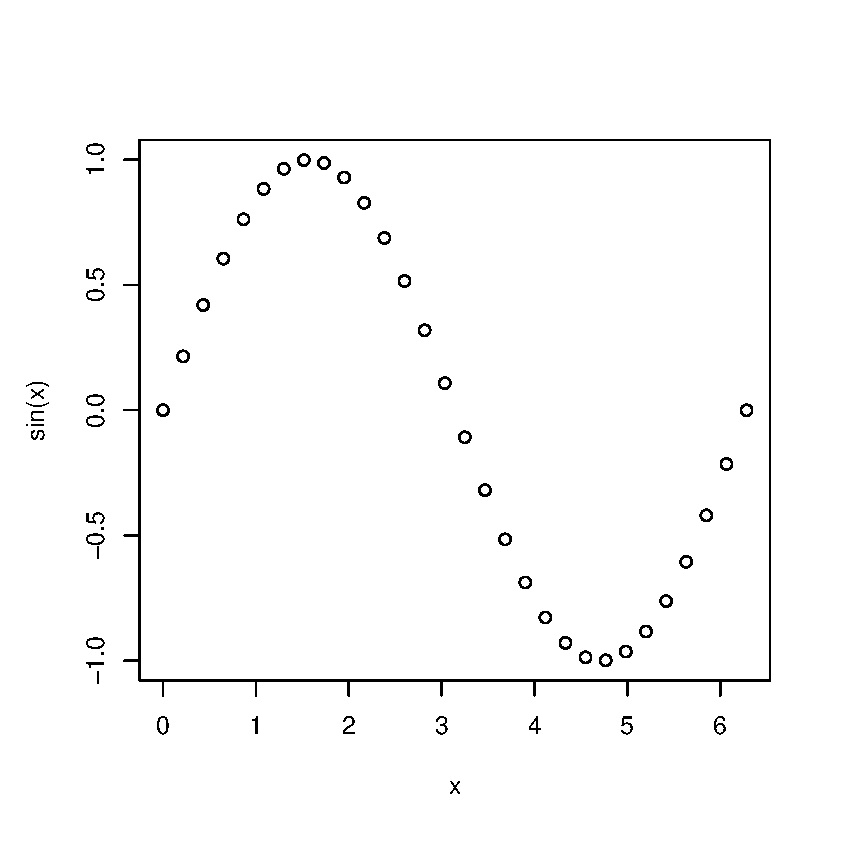
\includegraphics[width=3.0in]
{01Intro/Rplot01.eps}
\end{center}
\caption{ตัวอย่างจากคำสั่ง \texttt{plot}}
\label{fig: R plot}
\end{figure}
%

\section{แบบฝึกหัด}

\paragraph{1.} จงสืบค้นจากอินเตอร์เนตเพื่อหาตัวอย่างการประยุกต์ใช้การเรียนรู้ของเครื่องอย่างน้อย $3$ ตัวอย่าง.

\paragraph{2.} จากนิยามการเรียนรู้ของเครื่อง จงระบุประสบการณ์ $E$, งาน $T$, และตัววัดสมรรถนะ $P$ ของตัวอย่างจากข้อ 1.

\paragraph{3.} จงเขียนฟังชั่นเพื่อคำนวณค่าดอกเบี้ยทบต้น โดยรับอาร์กูเมนต์ $3$ ค่า คือเงินต้น ดอกเบี้ยต่อปี ($0$ ถึง $100\%$) และจำนวนปี เช่น
 \verb|compound(500000, 7, 20)| เพื่อคำนวณว่าเงินต้น $500,000$ บาท คิดดอกเบี้ยที่ $7\%$ ต่อปีทบต้น เป็นเวลา $20$ ปี พอจบปีที่ $20$ ยอดเงินรวมจะเป็นเท่าไร.

\paragraph{4.} จงเขียนโปรแกรมโดยใช้ฟังชั่น \texttt{plot} เพื่อให้ได้กราฟดังแสดงในรูป~\ref{fig: R plot ex1}.
สังเกตุการจัดรูปแบบ สี ลักษณะเส้น และชื่อกราฟ.
%สังเกตุในกราฟเป็นสีแดง และวาดทั้งเส้นและจุด รวมถึงมีชื่อกราฟแสดงด้วย.

%
\begin{figure}
\begin{center}
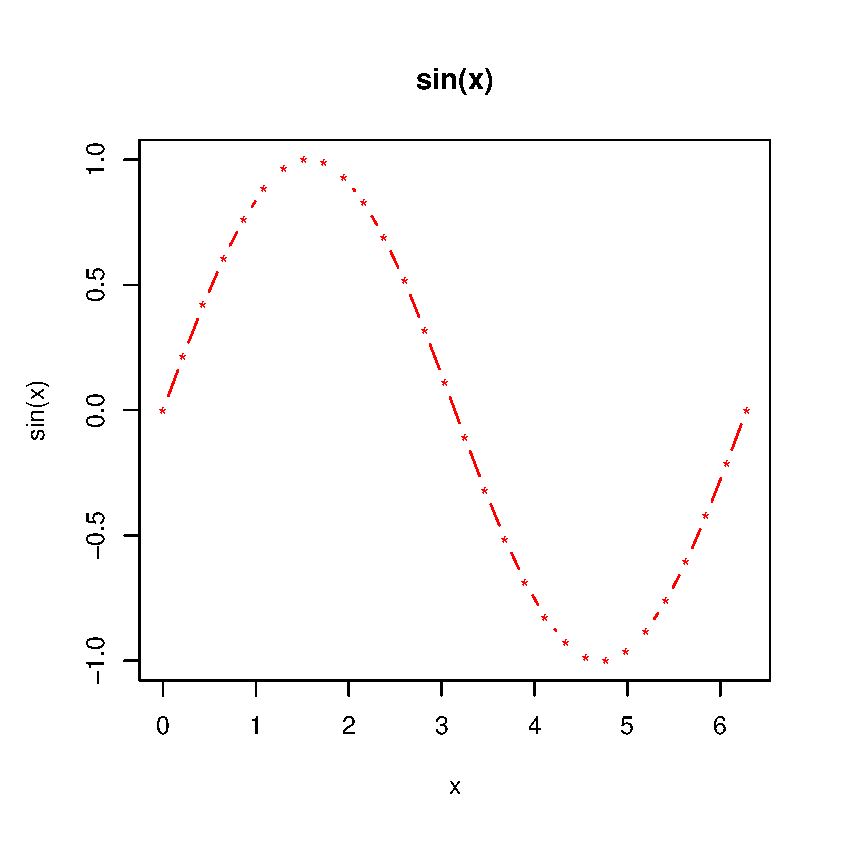
\includegraphics[width=3.0in]
{01Intro/RplotEx1.eps}
\end{center}
\caption{แบบฝึกหัด \texttt{plot} ข้อ 4}
\label{fig: R plot ex1}
\end{figure}
%

\paragraph{5.} จงศึกษาคำสั่ง \verb|par|, \verb|lines|, \verb|legend| และวาดกราฟดังแสดงในรูป~\ref{fig: R plot ex2}.
สังเกตุทั้งสองกราฟอยู่ในรูปเดียวกัน กราฟทางซ้ายมือแกน y มีค่าระหว่าง $-2$ ถึง $2$, ระบุชื่อของแกน y และ แกน x ตามรูป~\ref{fig: R plot ex2}.

%
\begin{figure}
\begin{center}
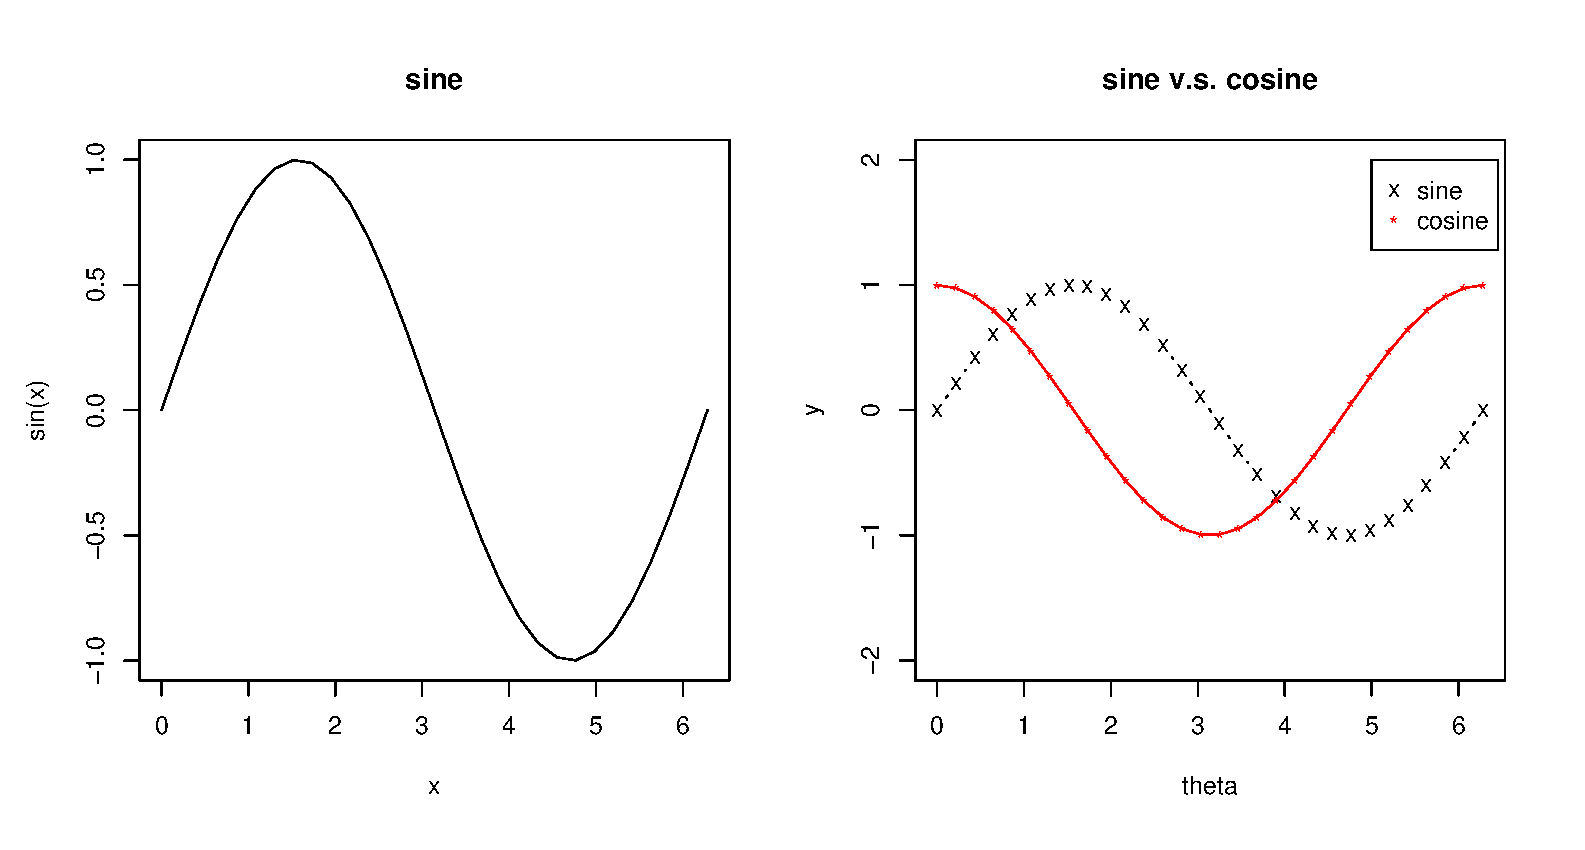
\includegraphics[width=6.0in]
{01Intro/RplotEx2.eps}
\end{center}
\caption{แบบฝึกหัด \texttt{plot} ข้อ 5}
\label{fig: R plot ex2}
\end{figure}
%

\paragraph{6.} โปรแกรมข้างล่างนี้ใช้วาดรูป~\ref{fig: R plot ex3}.
\begin{verbatim}
> x <- seq(0,100,len=5)
> plot(x, sin(x), type='l')
\end{verbatim}
จงวิเคราะห์และอธิบายว่าทำไมรูปที่ได้ไม่เห็นเป็นรูปโค้งขึ้นลงเหมือนรูปไซน์ที่คุ้นเคย.

%
\begin{figure}
\begin{center}
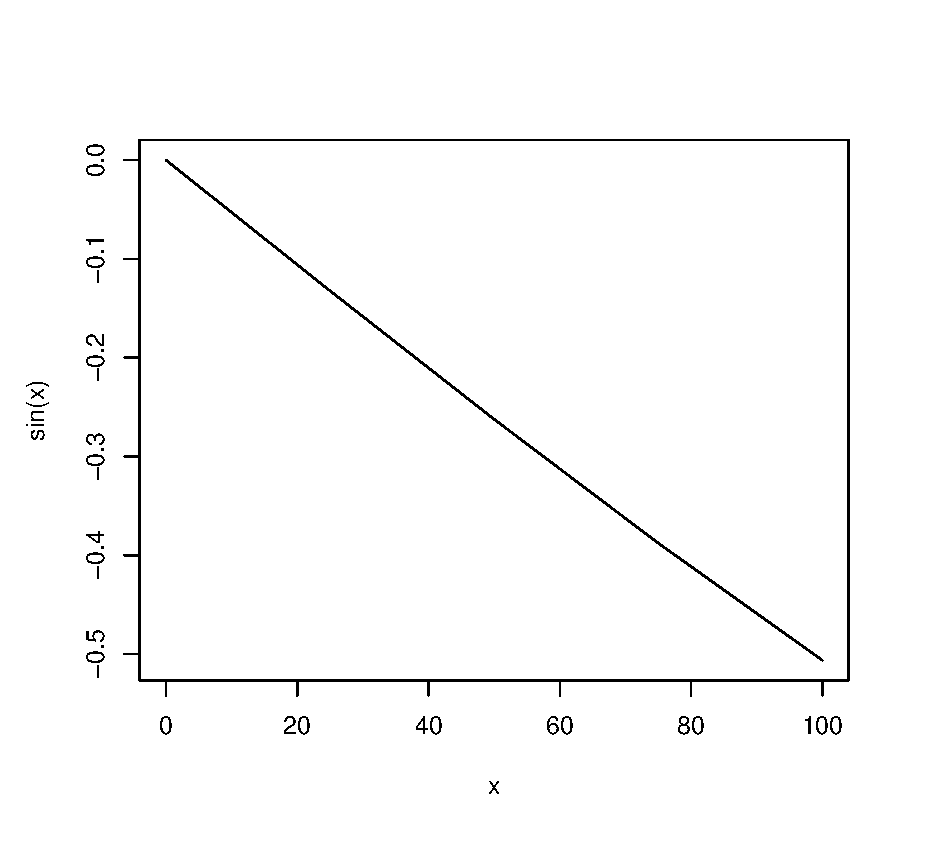
\includegraphics[width=3.0in]
{01Intro/RplotEx3.eps}
\end{center}
\caption{แบบฝึกหัดวิเคราะห์ข้อ 6}
\label{fig: R plot ex3}
\end{figure}
%

\paragraph{7.} โปรแกรมข้างล่างนี้ใช้วาดรูป~\ref{fig: R plot ex5}. 
\begin{lstlisting}[language=R,caption={โค้ดสำหรับรูปแบบฝึกหัดข้อ 7}]
x <- seq(-0.5, 0.5, len=50)

plot(x, 10*exp(-x^2)-8.8, type='l', ylab='y',
  main='10*exp(-x^2)-8.8 v.s. sin(x)')
lines(x, sin(x), col='red', lty=2)
legend(0, -0.5, c('10*exp(-x^2)-8.8', 'sin(x)'),
   lty=c(1,2), col=c('black', 'red'))
\end{lstlisting}
จงวิเคราะห์และอธิบายว่าทำไมกราฟเส้นประ ซึ่งเป็นกราฟของฟังชั่นไซน์จึงไม่เป็นรูปโค้งขึ้นลงเหมือนรูปไซน์ที่คุ้นเคย.

%
\begin{figure}
\begin{center}
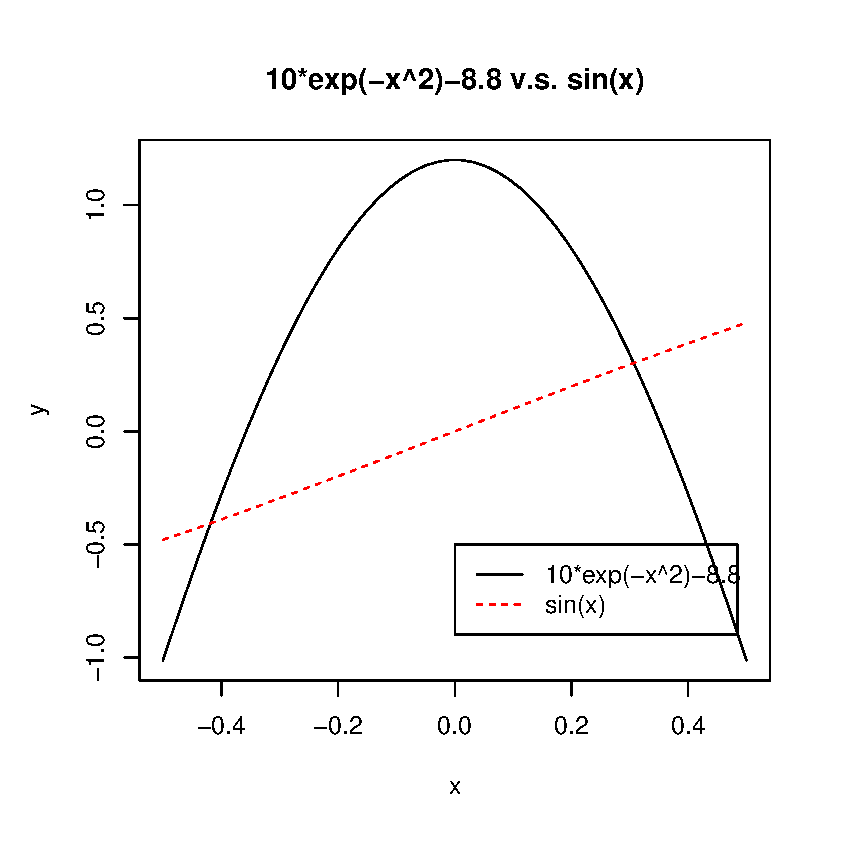
\includegraphics[width=3.0in]
{01Intro/RplotEx5.eps}
\end{center}
\caption{แบบฝึกหัดวิเคราะห์ข้อ 7}
\label{fig: R plot ex5}
\end{figure}
%

\paragraph{8.} จากโปรแกรมและผลการรันดังแสดงข้างล่างนี้
จงอภิปรายว่าทำไมมี $x$ บางตัวไม่เท่ากับ $7 \cdot y$ ซึ่ง $y = x/7$.
\begin{verbatim}
> x <- seq(1,10, len=20)
> y <- x/7
> x == 7*y
 [1]  TRUE  TRUE  TRUE  TRUE  TRUE  TRUE  TRUE  TRUE
 [9]  TRUE  TRUE  TRUE  TRUE  TRUE FALSE FALSE  TRUE
[17]  TRUE  TRUE  TRUE  TRUE
\end{verbatim}
จงวิเคราะห์และอธิบายผลของ \verb|x == 7*(x/7)| กับ \verb|x == 7*x/7| ประกอบ
พร้อมอภิปรายการประยุกต์ใช้ประเด็นที่ได้เรียนรู้นี้กับสถานการณ์ที่อาจจะเกิดขึ้น รวมถึงความเสี่ยงและโอกาส.

\paragraph{9.} %%จากคณิตศาสตร์ $\log( \exp(x) ) = x$ และ $\log(A/B) = \log(A) - \log(B)$, 
โปรแกรมข้างล่างนี้วาดรูป~\ref{fig: R plot ex6}.
\lstinputlisting[language=R,caption={โปรแกรมสำหรับรูปแบบฝึกหัดข้อ 9}]{01Intro/introQ9Code.r}

รูปบนเป็นกราฟของ $x^2$ (เส้นทึบสีดำ) และ $x^2 - x^2$ (เส้นประสีแดง).
รูปล่างเป็นกราฟของ $\log(\exp(x^2))$ (เส้นทึบสีดำ) และ $\log(\exp(x^2)/\exp(x^2))$ (เส้นประสีแดง).
จากความรู้คณิตศาสตร์ จะได้ $\log(\exp(x^2)) = x^2$ และ $\log(\exp(x^2)/\exp(x^2)) = x^2 - x^2$ 
แต่ทำไมกราฟรูปบนจึงต่างจากรูปล่าง (รูปบนแสดงค่าไปจนถึง $x = 30$ แต่รูปล่างไม่ถึง). 
จงอภิปราย.

%
\begin{figure}
\begin{center}
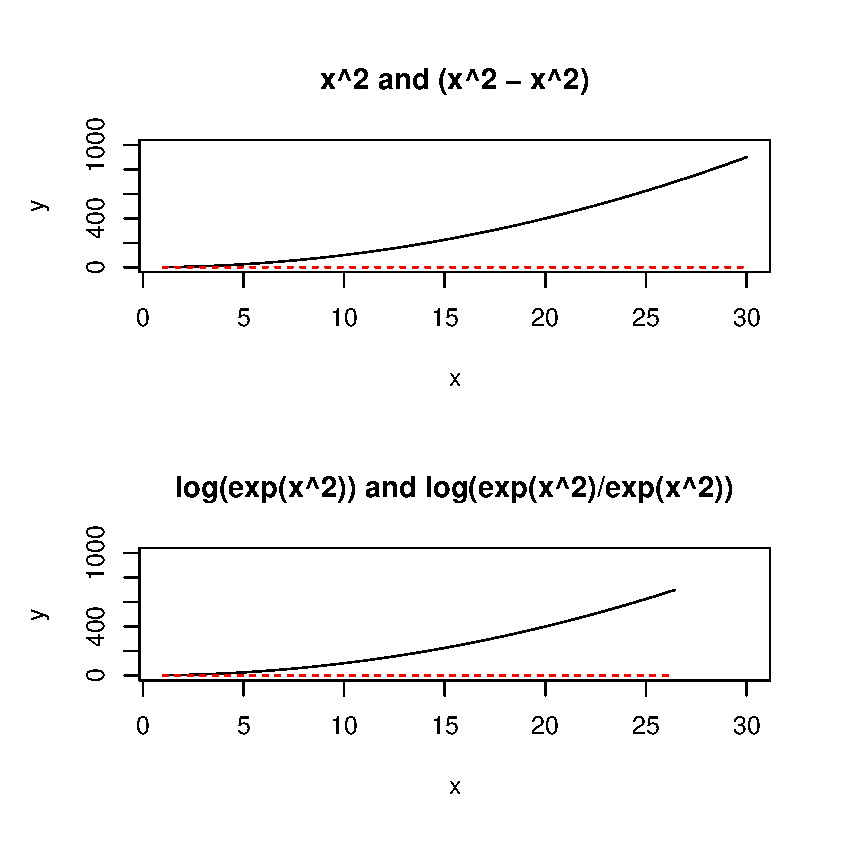
\includegraphics[width=4.0in]
{01Intro/RplotEx6.eps}
\end{center}
\caption{แบบฝึกหัดวิเคราะห์ข้อ 9}
\label{fig: R plot ex6}
\end{figure}
%

\paragraph{10.} จงศึกษาผลจากการคูณกันของเวกเตอร์ทิศทางต่างๆ.
จากโปรแกรมอาร์โปรเจคข้างล่าง ทดลองดูผลการคูณกันของเวกเตอร์ $2$ เวกเตอร์
นั่นคือ \verb|vq1| กับ \verb|v2|
โดย \verb|vq1| จะอยู่ที่เดิม แต่ \verb|v2| จะเปลี่ยนทิศทางไป ($20$ ค่ารอบทิศทาง ตั้งแต่ $\frac{1}{10}\pi$ จนถึง $2 \pi$).
โปรแกรมจะวาดรูปออกมา $2$ รูป 
แต่ละรูปแสดง $10$ ภาพย่อย
รวมทั้งหมด $20$ ภาพย่อย (แต่ละภาพย่อยแทนแต่ละทิศทางของ \verb|v2|).
สังเกตุผลจากการคูณ ที่ระบุไว้ในแต่ละภาพ และทดลองเปลี่ยนค่าองศาของ \verb|vq1| ให้เป็นค่าอื่นๆ (เปลี่ยนค่าของ \verb|theta1| ที่ตอนนี้ระบุเป็น \verb|6*pi/10|)
สรุปผลจากการคูณเวกเตอร์ทิศทางต่างๆ และตอบคำถาม ก.-จ. (เวกเตอร์ทุกตัวมีขนาดมากกว่า $0$)
\lstinputlisting[language=R,caption={โปรแกรมวาดรูปสำหรับแบบฝึกหัดข้อ 10}]{01Intro/introQ10Code.r}


\begin{itemize}
\item ก. ถ้าเวกเตอร์ A คูณกับเวกเตอร์ B ได้ผลเป็นบวก และเวกเตอร์ A ชี้ไปทิศทางสองนาฬิกา (เทียบเท่า $30$ องศาจากแกน $x$) สิ่งนี้บอกอะไรได้บ้างเกี่ยวกับทิศทางของเวกเตอร์ B

\item ข. ถ้าเวกเตอร์ A จากข้อ ก. ขนานกับเวกเตอร์ C ผลคูณของเวกเตอร์ A กับ C ผลคูณนี้จะเป็นอะไรได้บ้าง และเป็นอะไรไม่ได้บ้าง

\item ค. ถ้าเวกเตอร์ A จากข้อ ก. ตั้งฉากกับเวกเตอร์ D ผลคูณของเวกเตอร์ A กับ D ผลคูณนี้จะเป็นอะไรได้บ้าง และเป็นอะไรไม่ได้บ้าง

\item ง. ถ้าเวกเตอร์ A จากข้อ ก. คูณกับเวกเตอร์ E ได้ผลเป็นลบ
สิ่งนี้บอกอะไรได้บ้างเกี่ยวกับทิศทางของเวกเตอร์ E

\item จ. ถ้าหากต้องการผลคูณเวกเตอร์ A จากข้อ ก. กับเวกเตอร์ F ให้ได้ผลเป็นบวกและมีค่ามากที่สุด เวกเตอร์ F ควรมีทิศทางอย่างไร
\end{itemize}

 %done

%% Optimization
\chapter{การหาค่าดีที่สุด}
\label{chapter: Optimization}
\index{Optimization}
\index{การหาค่าดีที่สุด}


%\begin{verse}
%``Some progress quickly with a lot of pain, and others progress quickly with a lot of pleasure. It very much depends on our past accumulations of karma, how developed our spiritual faculties of mind already are. But if we’re facing in the right direction, all we have to do is keep on walking. If it takes a year, or sixty years, or five lifetimes, as long as we’re heading towards light, that’s all that matters.''
%Joseph Goldstein’s The Experience of Insight 
%\end{verse}

\begin{verse}
``... if we’re facing in the right direction, \\
all we have to do is keep on walking.'' \\
---Joseph Goldstein’s The Experience of Insight 
\end{verse}

\begin{verse}
``... ถ้าเรามุ่งหน้าไปในทิศทางที่ถูกต้อง \\
สิ่งที่เราต้องทำก็แค่เดินไปเรื่อยๆ'' \\
---ประสบการณ์แห่งความเข้าใจที่ลึกซึ้ง โจเซฟ โกล์ดสไตน์ 
\end{verse}

\textit{การเรียนรู้ของเครื่อง}ในมุมมองหนึ่งก็คือ\textit{การสร้างโมเดล}และ\textit{การหาค่าพารามิเตอร์ที่ดีที่สุด}ให้กับโมเดล โดยอาศัยประสบการณ์ที่เกี่ยวข้องช่วย.
การหาค่าพารามิเตอร์ที่ดีที่สุดสามารถใช้เทคนิคและความรู้จากศาสตร์และศิลป์ของวิชา\textit{การหาค่าดีที่สุด} (Optimization) มาช่วยได้.
วิชาการหาค่าดีที่สุดมีรายละเอียดมาก และด้วยเนื้อหาของวิชาการหาค่าดีที่สุดเองก็มากพอที่จะเป็นตำราของตัวเองได้.
บทนี้จะถกถึงเฉพาะพื้นฐานบางส่วนของศาสตร์การหาค่าดีที่สุดที่พอจะช่วยให้เข้าใจกระบวนการเกี่ยวข้องกับศาสตร์การเรียนรู้ของเครื่องบ้างเท่านั้น.

\section{การหาค่าดีที่สุดพื้นฐาน}
\label{section: Optimization}
\index{Optimization}
\index{การหาค่าดีที่สุด}

การหาค่าดีที่สุด (Optimization) คือการเลือกค่าของปัจจัย (แทนด้วยตัวแปร) ที่มีผลให้เป้าหมาย (แทนด้วยฟังชั่นของตัวแปร) มีค่าน้อย หรือมากที่สุด.
ปัจจัยที่ต้องการเลือก จะเรียกว่า \textit{ตัวแปรตัดสินใจ} (Decision Variable) และ
เป้าหมาย จะเรียกว่า \textit{ฟังชั่นจุดประสงค์} (Objective Function).
%
ตัวอย่างเช่น การเลือกเลือกค่าปัจจัยอุณหภูมิ แทนด้วยตัวแปร $x$ เพื่ออบมะเขือเทศได้อร่อยที่สุด โดยวัดจากปริมาณน้ำตาลที่ได้มากที่สุด โดยฟังชั่น $h$ แสดงความสัมพันธ์ระหว่างอุณหภูมิกับปริมาณน้ำตาลที่ได้จากการอบมะเขือเทศ.
ตัวแปร $x$ คือตัวแปรตัดสินใจ และฟังชั่น $h$ คือฟังชั่นจุดประสงค์.
กรณีนี้คือ การหาค่า $x$ ที่ทำให้ได้ค่าฟังชั่น $h$ มากที่สุด.
%ตัวอย่างเช่น การเลือกเลือกค่าตัวแปรนำ้หนัก $w_0$ กับ $w_1$ เพื่อให้ค่าความผิดพลาดจากการประมาณน้อยที่สุด.
%ตัวแปร $w_0$ กับ $w_1$ คือตัวแปรตัดสินใจ (ในกรณีนี้ มี $2$ ตัวแปร)
%และ\textit{ฟังชั่นค่าความผิดพลาด} (สมการ~\ref{eq: bg curve fitting E}) คือฟังชั่นจุดประสงค์.

ปัญหาที่เป็นการหาค่าที่ทำให้เป้าหมายมีค่ามากที่สุด เรียกรวมๆว่า \textit{ปัญหาค่ามากที่สุด} (Maximization Problem).
ตัวอย่างการเลือกอุณหภูมิการอบมะเขือเทศเพื่อให้ได้ปริมาณน้ำตาลสูงสุด เป็น\textit{ปัญหาค่ามากที่สุด}.
การเลือกชนิดการลงทุนเพื่อให้ได้ผลตอบแทนมากที่สุด 
การเลือกความเร็วของรถเพื่อวิ่งได้ระยะทางไกลที่สุด (ระยะทางมากที่สุด) สำหรับนำ้มัน $1$ ถัง 
เหล่านี้เป็นตัวอย่างของ\textit{ปัญหาค่ามากที่สุด}.

ทำนองเดียวกัน ปัญหาที่เป็นการหาค่าที่ทำให้เป้าหมายมีค่าน้อยที่สุด เรียกรวมๆว่า \textit{ปัญหาค่าน้อยที่สุด} (Minimization Problem).
ตัวอย่างเช่น การเลือกเส้นทางขับรถจากขอนแก่นไปร้อยเอ็ด โดยใช้เวลาเดินทางให้น้อยที่สุด.

ในทางคณิตศาสตร์ ปัญหาค่าน้อยที่สุดกับปัญหาค่ามากที่สุด สามารถแปลงไปมาระหว่างกันได้.
นั่นคือ การหาค่า $x$ ที่ทำให้ $h(x)$ มีค่ามากที่สุด 
จะเทียบเท่ากับ การหาค่า $x$ ที่ทำให้ $-h(x)$ มีค่าน้อยที่สุด (ดูแบบฝึกหัดการหาค่าดีที่สุด).
ดังนั้น เพื่อความสะดวก ปัญหาการหาค่าดีที่สุด ไม่ว่าจะเป็นปัญหาค่าน้อยที่สุดหรือปัญหาค่ามากที่สุด ก็สามารถเขียนให้อยู่ในรูปปัญหาค่าน้อยที่สุด ได้ดังนี้
\begin{eqnarray}
   \underset{\mathbf{x}}{\mbox{minimize}} & g(\mathbf{x})
\nonumber \\
   \mbox{subject to} & \mathbf{x} \in \Omega
\end{eqnarray}
โดย $\mathbf{x}$ คือตัวแปรตัดสินใจ (ซึ่งอาจมีหลายมิติ $\mathbf{x} = [x_1, x_2, \ldots, x_n]^T \in \mathbb{R}^n$),
$g: \mathbb{R}^n \to \mathbb{R}$ เป็นฟังชั่นจุดประสงค์ (หรือ Cost Function),
และเซต $\Omega$ เป็นซับเซตของ $\mathbb{R}^n$ ที่ระบุค่าของตัวแปรในช่วงที่สนใจหรือยอมรับได้ เรียกว่า เซตข้อจำกัด (Constraint Set หรือ Feasible Set).
ถ้า $\Omega = \mathbb{R}^n$ (หรือไม่มีข้อจำกัดของตัวแปรตัดสินใจ) จะเรียกปัญหาแบบนี้ว่า \textit{ปัญหาหาค่าดีที่สุดแบบไม่มีข้อจำกัด} (Unconstrained Optimization Problem).
เพื่อความสะดวก ค่าตัวแปรตัดสินใจที่ทำให้ฟังชั่นเป้าหมายมีค่าน้อยที่สุด จะเรียกว่า \textit{ค่าทำน้อยที่สุด} (Minimizer) และนิยมใช้ตัวยกดอกจันทร์ตามตัวแปร เช่น $\mathbf{x}^*$ เพื่อระบุว่า กำลังพูดถึง\textit{ค่าทำน้อยที่สุด}.

เมื่อพูดถึงการหาค่าน้อยที่สุด สิ่งที่ต้องการคือ ค่าทำน้อยที่สุดและค่าฟังชั่นเป้าหมายของมัน (ซึ่งน้อยที่สุด).
ค่าทำน้อยที่สุด มี $2$ ประเภท ได้แก่ ค่าทำน้อยที่สุดท้องถิ่น และ ค่าทำน้อยที่สุดทั่วหมด.

\paragraph{นิยามของค่าทำน้อยที่สุดท้องถิ่น.}
สมมติ $g: \mathbb{R}^n \to \mathbb{R}$ เป็นฟังชั่นค่าจริงที่นิยามสำหรับเซต $\Omega \subset \mathbb{R}^n$. 
จุด $\mathbf{x}^* \in \Omega$ เป็นค่าทำน้อยที่สุดท้องถิ่น (Local Minimizer) ของ $g$ บนเซต $\Omega$ ถ้ามีค่า $\epsilon > 0$ ที่ $g(\mathbf{x}) \geq f(\mathbf{x}^*)$ สำหรับ ทุกค่า $\mathbf{x} \in \Omega \setminus \{ \mathbf{x}^*\}$ และ $\| \mathbf{x} - \mathbf{x}^* \| < \epsilon$.

\paragraph{นิยามของค่าทำน้อยที่สุดทั่วหมด.}
จุด $\mathbf{x}^* \in \Omega$  เป็นค่าทำน้อยที่สุดทั่วหมด (Global Minimizer) ของฟังชั่น $g$ บนเซต $\Omega$ ถ้า $g(\mathbf{x}) \geq g(\mathbf{x}^*)$ สำหรับทุก $\mathbf{x} \in \Omega \setminus \{\mathbf{x}^*\}$.

จากนิยามข้างต้น กล่าวง่ายๆก็คือ 
\textit{ค่าทำน้อยที่สุดท้องถิ่น}คือค่าตัวแปรตัดสินใจที่ให้ค่าเป้าหมายน้อยกว่าค่าเป้าหมายบริเวณรอบๆ (ท้องถิ่น).
ส่วน \textit{ค่าทำน้อยที่สุดทั่วหมด}คือค่าตัวแปรตัดสินใจที่ให้ค่าเป้าหมายน้อยกว่าค่าเป้าหมายของทุกๆค่าตัวแปรตัดสินใจที่เป็นไปได้ (ทั่วทั้งหมด).
ดังนั้น \textit{ค่าทำน้อยที่สุดทั่วหมด} ก็จะเป็น\textit{ค่าทำน้อยที่สุดท้องถิ่น}ด้วยเสมอ.
รูป~\ref{fig: minimizers} แสดงค่าทำน้อยที่สุดต่างๆ โดย 
\texttt{x1} เป็นทั้งค่าทำน้อยที่สุดทั่วหมดและค่าทำน้อยที่สุดท้องถิ่น
ส่วน \texttt{x2} ถึง \texttt{x6} เป็นค่าทำน้อยที่สุดท้องถิ่น.

%
\begin{figure}
\begin{center}
\includegraphics[height=3.0in]
{02Background/minimizers.eps}
\end{center}
\caption{ค่าทำน้อยที่สุดต่างๆ}
\label{fig: minimizers}
\end{figure}
%

\section{เงื่อนไขของค่าทำน้อยที่สุดท้องถิ่น}
\label{sec: opt FONC}

จากฟังชั่นเป้าหมาย $g: \mathbb{R}^n \mapsto \mathbb{R}$ อนุพันธ์อันดับหนึ่งของฟังชั่นเป้าหมาย เขียนย่อเป็น $D g$, คือ
\begin{eqnarray}
   D g = \left[ \frac{\partial g}{\partial x_1}, 
                \frac{\partial g}{\partial x_2},
                \ldots,
                \frac{\partial g}{\partial x_n}
         \right]
\end{eqnarray}
และเกรเดียนต์ (Gradient) $\nabla g = (D g)^T$.

อนุพันธ์อันดับสองของฟังชั่นเป้าหมาย เรียกว่า \textit{เฮเชียน} (Hessian of $g$) คือ
\begin{eqnarray}
   \mathbf{G}(\mathbf{x}) = D^2 g(\mathbf{x}) = 
   \begin{bmatrix}
   \frac{\partial^2 g}{\partial x_1^2} (\mathbf{x}) & \cdots & \frac{\partial^2 g}{\partial x_n x_1} (\mathbf{x}) \\
   \vdots    &        & \vdots \\
   \frac{\partial^2 g}{\partial x_1 x_n} (\mathbf{x}) & \cdots & \frac{\partial^2 g}{\partial x_n^2} (\mathbf{x})   
   \end{bmatrix}
\end{eqnarray}

\begin{myexample}
เช่น ถ้า $g(\mathbf{x}) = 2 x_1 + 18 x_2 + x_1 x_2 - x_1^2 - 4 x_2^2$, ดังนั้น
\begin{eqnarray}
   \nabla g (\mathbf{x}) = \begin{bmatrix}
   \frac{\partial g}{\partial x_1} (\mathbf{x}) \\
   \frac{\partial g}{\partial x_2} (\mathbf{x})   
   \end{bmatrix}
   = 
   \begin{bmatrix}
   2 + x_2 - 2 x_1 \\
   18 + x_1 - 8 x_2
   \end{bmatrix}   
\nonumber   
\end{eqnarray}
และ
\begin{eqnarray}
   \mathbf{G}(\mathbf{x}) = D^2 g(\mathbf{x}) = 
   \begin{bmatrix}
   \frac{\partial^2 g}{\partial x_1^2}(\mathbf{x}) & 
     \frac{\partial^2 g}{\partial x_2 x_1}(\mathbf{x}) \\
   \frac{\partial^2 g}{\partial x_1 x_2}(\mathbf{x}) & 
     \frac{\partial^2 g}{\partial x_2^2}(\mathbf{x})
   \end{bmatrix}
   = \begin{bmatrix}
   -2 & 1 \\
   1 & -8
   \end{bmatrix}
\nonumber
\end{eqnarray}
\end{myexample}


จากเซตข้อจำกัด $\Omega$ \textit{ค่าทำน้อยที่สุด}อาจจะอยู่ภายใน $\Omega$ (กรณีนี้เรียกว่า กรณีภายใน,  Interior Case) หรืออาจจะอยู่ที่ขอบของ $\Omega$ ก็ได้ (กรณีขอบเขต, Boundary Case).

เพื่อความสะดวกการศึกษาทั้งสองกรณี โดยเฉพาะกรณีขอบเขต เราจะนำแนวคิดของ\textit{ทิศทางซึ่งเป็นไปได้} 
(Feasible Direction) เข้ามา.

\paragraph{นิยามทิศทางซึ่งเป็นไปได้.}\index{ทิศทางซึ่งเป็นไปได้}\index{Feasible Direction}
เวกเตอร์ $\mathbf{d} \in \mathbb{R}^n, \mathbf{d} \neq \mathbf{0}$ เป็น\textit{ทิศทางซึ่งเป็นไปได้} 
(Feasible Direction) ที่ $\mathbf{x} \in \Omega$ ก็ต่อเมื่อมีค่า $\alpha_0 > 0$ ที่ทำให้ $\mathbf{x} + \alpha \mathbf{d} \in \Omega$ สำหรับทุกๆค่าของ $\alpha \in [0, \alpha_0]$.
%
ดูรูป~\ref{fig: feasible direction} และ \ref{fig: feasible directions at different points} ประกอบ.

%
\begin{figure}
\begin{center}
\includegraphics[width=2.0in]
{02Background/feasibleDirection01.png}
\end{center}
\caption{รูปประกอบช่วยอธิบาย\textit{ทิศทางซึ่งเป็นไปได้}. 
ทิศทาง $d_1$ ไม่ใช่\textit{ทิศทางซึ่งเป็นไปได้} 
ทิศทาง $d_2$ คือ\textit{ทิศทางซึ่งเป็นไปได้}ที่ $x$}
\label{fig: feasible direction}
\end{figure}
%


%
\begin{figure}
\begin{center}
\includegraphics[width=4.0in]
{02Background/feasibleDirections.eps}
\end{center}
\caption{\textit{ทิศทางซึ่งเป็นไปได้}ที่จุดต่างๆ 5 จุด 
ได้แก่ \texttt{P1} ถึง \texttt{P5} ภายใน\textit{เซตข้อจำกัด} (ภายในพื้นที่แรเงา). เส้นเล็กที่วาดออกมาจากแต่ละจุด คือ ตัวอย่างของ\textit{ทิศทางซึ่งเป็นไปได้}ต่างๆที่จุดนั้น 
เช่นที่จุด \texttt{P1} ที่อยู่ชิดขอบล่างของ\textit{เซตข้อจำกัด} มี\textit{ทิศทางซึ่งเป็นไปได้}ต่างๆ ได้ตั้งแต่ทิศทางสามนาฬิกาทวนเข็มไปจนถึงเก้านาฬิกา).
สังเกตุ\textit{ทิศทางซึ่งเป็นไปได้}ต่างๆ ที่จุดที่อยู่ขอบของ\textit{เซตข้อจำกัด} (อาทิ จุด \texttt{P1}, \texttt{P2}, \texttt{P3}, \texttt{P5}) เทียบกับ จุด \texttt{P4} ที่อยู่ภายใน\textit{เซตข้อจำกัด}. 
หมายเหตุ เพื่อความสะดวกหัวเวกเตอร์วาดด้วยจุดแทนลูกศร}
\label{fig: feasible directions at different points}
\end{figure}
%

จากนิยาม\textit{ทิศทางซึ่งเป็นไปได้} เพื่อศึกษาคุณสมบัติหรือเงื่อนไขที่สามารถใช้ช่วยในการแก้ปัญหาการหาค่าน้อยที่สุด
พิจารณาการวิเคราะห์ต่อไปนี้.

ถ้าให้ ฟังชั่นค่าจริง $g: \mathbb{R}^n \mapsto \mathbb{R}$ และ $\mathbf{d}$ เป็น\textit{ทิศทางซึ่งเป็นไปได้}ที่ $\mathbf{x} \in \Omega$ แล้ว\textit{อนุพันธ์เชิงทิศทาง} (Directional Derivative) ของ $g$ ในทิศทาง $\mathbf{d}$ ซึ่งเขียนย่อด้วย $\partial g/\partial \mathbf{d}$, คือ
\begin{eqnarray}
   \frac{\partial g}{\partial \mathbf{d}} (\mathbf{x}) = \lim_{\alpha \to 0} \frac{g(\mathbf{x} + \alpha \mathbf{d}) - g(\mathbf{x})}{\alpha}.
\end{eqnarray}

ถ้า $\| d \| = 1$ แล้ว ค่า $\partial g/\partial \mathbf{d}$ ก็คือ อัตราการเพิ่มของค่าฟังชั่น $g$ ที่ $\mathbf{x}$ ในทิศทางของ $\mathbf{d}$ นั่นเอง.

สำหรับการคำนวณค่า $\partial g/\partial \mathbf{d}$ 
สมมติว่ามีค่า $\mathbf{x}$ กับ $\mathbf{d}$ อยู่ 
ดังนั้น $g(\mathbf{x} + \alpha \mathbf{d})$ เป็นฟังชั่นของ $\alpha$ หรือ
\begin{eqnarray}
   \frac{\partial g}{\partial \mathbf{d}} (\mathbf{x}) =
   \left. 
   \frac{d}{d \alpha} g(\mathbf{x} + \alpha \mathbf{d}) 
   \right|_{\alpha=0}
\nonumber
\end{eqnarray}
เมื่อใช้\textit{กฏลูกโซ่} (Chain Rule) เข้าไป จะได้
\begin{eqnarray}
\frac{d g(\mathbf{x} + \alpha \mathbf{d})}{d \alpha}
=
\frac{d g(\mathbf{x} + \alpha \mathbf{d})}{d (\mathbf{x} + \alpha \mathbf{d})} \cdot \frac{d (\mathbf{x} + \alpha \mathbf{d})}{d \alpha} 
%\nonumber \\
= (\nabla g(\mathbf{x})^T) \cdot (\mathbf{d}) = \mathbf{d}^T \nabla g(\mathbf{x}).
\nonumber
\end{eqnarray}

\paragraph{First-Order Necessary Condition (FONC).} \textit{เงื่อนไงจำเป็นอันดับแรก} (ของตัวทำต่ำสุด) คือ
ให้ $\Omega \subset \mathbb{R}^n$ และ $g \in \mathcal{C}^1$ เป็นฟังชั่นค่าจริงบนเซต $\Omega$ แล้ว
ถ้า $\mathbf{x}^*$ เป็น\textit{ตัวทำต่ำสุดท้องถิ่น}ของฟังชั่น $g$ บนเซต $\Omega$ แล้ว 
สำหรับแต่ละ\textit{ทิศทางซึ่งเป็นไปได้} $\mathbf{d}$ ที่ $\mathbf{x}^*$ ต้องได้ว่า
อนุพันธ์เชิงทิศทางที่จุดนั้นต้องมากกว่าหรือเท่ากับศูนย์. 
นั่นคือ
\begin{eqnarray}
   \mathbf{d}^T \nabla g(\mathbf{x}^*) \geq 0
\label{eq: FONC}
\end{eqnarray}
สำหรับทุกๆ $\mathbf{d}$.
%(ดูเพิ่มเติม โดยเฉพาะเรื่องพิสูจน์จาก \citet{ChongZak2ndEd}
หมายเหตุ $g \in \mathcal{C}^1$ หมายถึง ฟังชั่น $g$ เป็นฟังชั่นค่าต่อเนื่อง และมีอนุพันธ์อันดับหนึ่งทุกจุดบนเซตจำกัด.

รูป~\ref{fig: FONC} (รูปล่าง) แสดง\textit{ค่าทำน้อยที่สุด}ที่จุด \texttt{x1} (ที่ขอบซ้ายของเซตข้อจำกัด) พร้อมเกรเดียนต์ (\texttt{v1}) และตัวอย่าง\textit{ทิศทางซึ่งเป็นไปได้} (\texttt{d1} กับ \texttt{d2}) ซึ่งเมื่อตรวจคุณสมบัติจะได้ตาม\textit{เงื่อนไงจำเป็นอันดับแรก} (FONC).

เมื่อพิจารณาเปรียบเทียบกับจุด \texttt{x2} ที่ขอบขวาของเซตข้อจำกัด 
ที่จุด \texttt{x2} มีเกรเดียนต์ (\texttt{v2}) 
และตัวอย่าง\textit{ทิศทางซึ่งเป็นไปได้} (\texttt{d3}),
จุด \texttt{x2} ไม่ผ่าน\textit{เงื่อนไงจำเป็นอันดับแรก} เพราะมี\textit{ทิศทางซึ่งเป็นไปได้} \texttt{d3} ที่ทำให้ $\mathbf{d}_3 \nabla f(\mathbf{x}_2) < 0$ (สังเกตุ ทิศทางของเวกเตอร์ \texttt{v2} และ \texttt{d3}).
เมื่อไม่ผ่าน\textit{เงื่อนไงจำเป็นอันดับแรก} จึงมั่นใจได้ว่า จุด \texttt{x2} ไม่ใช่ค่าทำน้อยที่สุด.


%
\begin{figure}
\begin{center}
\includegraphics[width=6.0in]
{02Background/FONC.eps}
\end{center}
\caption{รูปบนซ้ายแสดงฟังชั่นเป้าหมายที่วาดแบบสามมิติ.
รูปบนขวาแสดงค่าฟังชั่นเป้าหมายที่วาดแบบคอนทัวร์ พร้อมแสดงเซตข้อจำกัด (พื้นที่ภายในวงกลมพื้นลาย), กากบาทสีแดงที่ $(5,3)$ คือ จุดที่ฟังชั่นเป้าหมายมีค่าน้อยที่สุด (แต่อยู่นอกเซตข้อจำกัด).
รูปล่างแสดงภาพขยายของรูปบนขวา โดยขยายเพื่อเน้นบริเวณเซตข้อกำจัด.
ที่จุด \texttt{x1} เป็น \textit{ค่าทำน้อยที่สุด}.
สังเกตุ ความสัมพันธ์ระหว่างเกรเดียนต์ (เวคเตอร์ \texttt{v}) กับทิศทางซึ่งเป็นไปได้ (เวคเตอร์ \texttt{d}) เปรียบเทียบความสัมพันธ์นี้ระหว่างจุด \texttt{x1} (ค่าทำน้อยที่สุด) กับ จุด \texttt{x2} ที่ขอบของเซตข้อจำกัดอีกด้าน}
\label{fig: FONC}
\end{figure}
%

\paragraph{เงื่อนไงจำเป็นอันดับแรกสำหรับกรณีภายใน.} 
ให้ $\Omega \subset \mathbb{R}^n$ และ $g \in \mathcal{C}^1$ เป็นฟังชั่นค่าจริงบนเซต $\Omega$ แล้ว
ถ้า $\mathbf{x}^*$ เป็น ตัวทำต่ำสุดของฟังชั่น $g$ บนเซต $\Omega$ และ ถ้า $\mathbf{x}^*$ เป็นจุดที่อยู่ภายในของเซต $\Omega$
% ($\mathbf{x}^*$ is an interior point) 
แล้วดังนั้น
\begin{eqnarray}
   \nabla g(\mathbf{x}^*) = \mathbf{0}.
\label{eq: FONC interior case}
\end{eqnarray}

%\begin{minipage}{5in}
%{\small
%\begin{shaded}
%\paragraph{ตัวอย่าง.}
\begin{myexample}
ปัญหาการค่าดีที่สุด
\begin{eqnarray}
  & \mbox{minimize}_{x_1, x_2} & 
     g(x_1, x_2) = x_1^2 + 0.5 x_2^2 + 3 x_2 + 73 
     \nonumber \\
  & \mbox{subject to } &
     x_1, x_2 \geq 0.
     \nonumber
\end{eqnarray}

รูป~\ref{fig: FONC example} แสดงค่าฟังชั่นเป้าหมายพร้อมขอบเขตของเซตข้อจำกัด.
ลองตรวจสอบเงื่อนไงจำเป็นอันดับแรกของจุด $(4,3), (3,0), (0,0)$ ดูว่าเป็นอย่างไรบ้าง.
ค่าเกรเดียนต์ คือ $\nabla g(\mathbf{x}) = [2 x_1 , x_2 + 3]^T$.
\begin{itemize}
\item ที่จุด $(4,3)$, $\nabla g(\mathbf{x} = [4,3]^T) = [2 x_1 , x_2 + 3]^T = [8, 6]^T$ และ ที่จุด $(4,3)$ (เป็นจุดภายใน, interior point), $\nabla g(\mathbf{x}) = [8, 6]^T \neq \mathbf{0}$  ดังนั้นจุดนี้จึงไม่ผ่านเงื่อนไงจำเป็นอันดับแรก.
% เราสามารถหา $\mathbf{d}$ ที่ทำให้ $\mathbf{d}^T \nabla f(\mathbf{x})$ ได้ เช่น $\mathbf{d} = [-1, 0]$, ดังนั้น จุด $(4,3)$ ไม่ผ่าน FONC.

\item ที่จุด $(3,0)$, $\nabla g(\mathbf{x} = [3,0]^T) = [6,3]^T$,
ดังนั้น $\mathbf{d}^T \nabla g(\mathbf{x}) = 6 d_1 + 3 d_2$ 
โดย $\mathbf{d} = [d_1, d_2]^T$.
ถ้าจะผ่านเงื่อนไงจำเป็นอันดับแรก ค่าของ $6 d_1 + 3 d_2$ ต้อง $\geq 0$ สำหรับทุกค่าของ $\mathbf{d}$ ที่จุด $(3,0)$ หรือ $6 d_1 + 3 d_2 \geq 0 \equiv d_1 \geq - d_2/2$.
แต่พบว่า มี\textit{ทิศทางซึ่งเป็นไปได้}ที่จุด $(3,0)$ 
เช่น $\mathbf{d} = [-1,0]^T$ จะทำให้ $\mathbf{d}^T \nabla f = -6 < 0$
ทำให้ จุด $(3,0)$ ไม่ผ่านเงื่อนไงจำเป็นอันดับแรก
%ที่ทำให้ $\mathbf{d}^T \nabla f < 0$ 
%ดังแสดงใน
ดูรูป~\ref{fig: FONC example P(3,0)} ประกอบ. %,  ไม่ผ่าน FONC.

\item ที่จุด $(0,0)$, $\nabla f(\mathbf{x} = [0,0]^T) = [0,3]^T$,
ดังนั้น $\mathbf{d}^T \nabla f(\mathbf{x}) = 3 d_2$, 
ซึ่งที่จุด $(0,0)$, $d_2 \geq 0$ จึงทำให้ $\mathbf{d}^T \nabla f(\mathbf{x}) \geq 0$ สำหรับทุกๆ\textit{ทิศทางซึ่งเป็นไปได้}.
จุด $(0,0)$ จึงผ่านเงื่อนไงจำเป็นอันดับแรก.
\end{itemize}

%\end{shaded}
%}%small
%\end{minipage}
\end{myexample}

%
\begin{figure}
\begin{center}
\includegraphics[width=6.0in]
{02Background/FONCexample.eps}
\end{center}
\caption{รูปซ้ายแสดงฟังชั่นเป้าหมายที่วาดแบบสามมิติ.
รูปบนขวาแสดงค่าฟังชั่นเป้าหมายที่วาดแบบคอนทัวร์ พร้อมเซตข้อจำกัด (พื้นที่แรเงา)}
\label{fig: FONC example}
\end{figure}
%


%
\begin{figure}
\begin{center}
\includegraphics[width=4.0in]
{02Background/FONCExampleP30.eps}
\end{center}
\caption{ตัวอย่าง \textit{ทิศทางซึ่งเป็นไปได้}ที่จุด $(3,0)$.
ทิศทาง เช่น \texttt{[-1,0]} และ \texttt{[-0.85, 0.5]} 
จะทำให้ $\mathbf{d}^T \nabla f < 0$.}
\label{fig: FONC example P(3,0)}
\end{figure}
%

\paragraph{Second-Order Necessary Condition (SONC).} เงื่อนไขจำเป็นอันดับสอง (ของตัวทำต่ำสุด) คือ
ให้ $\Omega \subset \mathbb{R}^n$ และ $g \in \mathcal{C}^2$ เป็นฟังชั่นค่าจริงบนเซต $\Omega$,
ให้ $\mathbf{x}^*$ เป็น\textit{ตัวทำต่ำสุดท้องถิ่น}ของฟังชั่น $g$ บนเซต $\Omega$, สำหรับทุกๆ\textit{ทิศทางซึ่งเป็นไปได้} $\mathbf{d}$ ที่ $\mathbf{x}^*$, 
ถ้า $\mathbf{d}^T \nabla g(\mathbf{x}^*) = 0$, แล้ว
\begin{eqnarray}
   \mathbf{d}^T \mathbf{G}(\mathbf{x}^*) \mathbf{d} \geq 0,
\label{eq: SONC}
\end{eqnarray}
เมื่อ $\mathbf{G}$ เป็นเฮเชียนของ $g$.
หมายเหตุ $g \in \mathcal{C}^2$ หมายถึง ฟังชั่น $g$ เป็นฟังชั่นค่าต่อเนื่อง และมีอนุพันธ์อันดับสองทุกจุดบนเซตจำกัด (สามารถหาเฮเชียน $\mathbf{G}$ ได้).

\paragraph{เงื่อนไขจำเป็นอันดับสองสำหรับกรณีภายใน.} %SONC สำหรับ interior case}
ให้ $\mathbf{x}^*$ เป็นจุดที่อยู่ภายในเซตจำกัด $\Omega \subset \mathbb{R}^n$, ถ้า $\mathbf{x}^*$ เป็นตัวทำน้อยที่สุดท้องถิ่นของฟังชั่นเป้าหมาย $g: \Omega \to \mathbb{R}, g \in \mathcal{C}^2$, แล้ว
\begin{eqnarray}
   \nabla g(\mathbf{x}^*) = \mathbf{0},
\nonumber   
\end{eqnarray}
และ $\mathbf{G}(\mathbf{x}^*)$ เป็น\textit{บวกกึ่งแน่นอน} (Positive Semi-Definite, $\mathbf{G}(\mathbf{x}^*) \geq 0$) ซึ่งก็คือ
\begin{equation}
   \mathbf{d}^T \mathbf{G}(\mathbf{x}^*) \mathbf{d} \geq 0,
   \mbox{ for all } \mathbf{d} \in \mathbb{R}^n.   
\nonumber   
\end{equation}

%\begin{minipage}{5in}
%{\small
%\begin{shaded}
%\paragraph{ตัวอย่าง.}
\begin{myexample}
ฟังชั่นเป้าหมาย $g(x) = x^3$, ที่ $x = 0$ ค่า $g'(0) = 0$ และ $g''(0) = 0$ ดังนั้น ที่จุด $x = 0$ ผ่านทั้งเงื่อนไขจำเป็นอันดับหนึ่งและอันดับสอง.
แต่ $x=0$ ไม่ใช่ค่าทำน้อยที่สุด ดังแสดงในรูป~\ref{fig: x^3}.
%\end{shaded}
%}%small
%\end{minipage}
\end{myexample}

%
\begin{figure}
\begin{center}
\includegraphics[width=4.0in]
{02Background/SONCexample01.png}
\end{center}
\caption{ตัวอย่าง ค่าฟังชั่น $g(x) = x^3$}
\label{fig: x^3}
\end{figure}
%

%\begin{minipage}{5in}
%{\small
%\begin{shaded}
%\paragraph{ตัวอย่าง.}
\begin{myexample}
ฟังชั่นเป้าหมาย $g(\mathbf{x}) = x_1^2 - x_2^2$ มีเกรเดียนต์ $\nabla g(\mathbf{x}) = [2 x_1, -2 x_2]^T$ และ เฮเชียน 
\begin{eqnarray}
   \mathbf{G}(\mathbf{x}) = \begin{bmatrix}
      2 & 0 \\
      0 & -2
   \end{bmatrix}.
\nonumber   
\end{eqnarray}

ที่ $\mathbf{x} = [0,0]^T$, $\nabla g(\mathbf{x}) = \mathbf{0}$ ซึ่งผ่านเงื่อนไขจำเป็นอันดับหนึ่ง 
แต่ค่าเฮเชียนไม่ได้เป็น\textit{บวกกึ่งแน่นอน} 
เนื่องจาก มี\textit{ทิศทางซึ่งเป็นไปได้} ที่ทำให้ $\mathbf{d}^T \mathbf{G} \mathbf{d} < 0$ 
เช่น $\mathbf{d} = [0,1]^T$.
จุด $\mathbf{x} = [0,0]^T$ จึงไม่ผ่านเงื่อนไขจำเป็นอันดับสอง ซึ่งยืนยันว่าจุดนี้ไม่ใช่ตัวทำน้อยที่สุด.
รูป~\ref{fig: SONC example} แสดงค่าฟังชั่นเป้าหมายของตัวอย่างนี้.
%\end{shaded}
%}%small
%\end{minipage}

\end{myexample}

%
\begin{figure}
\begin{center}
\includegraphics[width=4.0in]
{02Background/SONCexample02.png}
\end{center}
\caption{ตัวอย่างค่าฟังชั่น $g(x) = x_1^2 - x_2^2$.
แกนตั้งเป็นค่าฟังชั่น $g(x)$.
จุด $(0,0)$ ผ่านเงื่อนไขจำเป็นอันดับหนึ่ง แต่ไม่ผ่านเงื่อนไขจำเป็นอันดับสอง.}
\label{fig: SONC example}
\end{figure}
%

สังเกตุว่า ถ้าจุดใดไม่ผ่านเงื่อนไขจำเป็น จุดนั้นไม่ใช่ตัวทำต่ำสุด.
แต่จุดที่ผ่านเงื่อนไขจำเป็น จุดนั้นอาจจะไม่ใช่ตัวทำต่ำสุดก็ได้.

\paragraph{Second-Order Sufficient Condition (SOSC), Interior Case} 
เงื่อนไขเพียงพออันดับสอง สำหรับกรณีภายใน คือ
ให้ $g \in \mathcal{C}^2$ และ $\mathbf{x}^*$ เป็นจุดที่อยู่ภายในเซตข้อจำกัด,
ถ้า $\nabla g(\mathbf{x}^*) = \mathbf{0}$ และ 
$\mathbf{G}(\mathbf{x}^*) > 0$ แล้ว $\mathbf{x}^*$ เป็นตัวทำน้อยสุดท้องถิ่นอย่างแท้จริง (Strict Local Minimizer) ของ $g$.

%\begin{minipage}{5in}
%{\small
%\begin{shaded}
%\paragraph{ตัวอย่าง.}
\begin{myexample}
ฟังชั่นเป้าหมาย $g(\mathbf{x}) = x_1^2 + x_2^2$, เกรเดียนต์ $\nabla g(\mathbf{x}) = [2 x_1, 2 x_2]^T$ 
และค่าเกรเดียนต์ จะเท่ากับ $\mathbf{0}$ ก็เมื่อ $\mathbf{x} = [0,0]^T$ เท่านั้น 
และเนื่องจากค่าเฮเชียนเป็น
\begin{eqnarray}
   \mathbf{G}(\mathbf{x}) = \begin{bmatrix}
      2 & 0 \\
      0 & 2
   \end{bmatrix}
\nonumber   
\end{eqnarray}
ซึ่งเป็น\textit{บวกแน่นอน} ($\mathbf{G} > 0$) เพราะ 
$\mathbf{d}^T \mathbf{G} \mathbf{d} = 2 d_1^2 + 2 d_2^2 > 0$ ไม่ว่าค่า $d_1$ หรือ $d_2$ จะเป็นอะไร ($d_1, d_2 \in \mathbb{R}$).
จุด $(0,0)$ ผ่านเงื่อนไขทั้งเงื่อนไขจำเป็นอันดับหนึ่ง อันดับสอง และเงื่อนไขเพียงพออันดับสอง, จุด $(0,0)$ จึงเป็น\textit{ตัวทำค่าน้อยที่สุด}ของฟังชั่นนี้ (รูป~\ref{fig: SOSC example} แสดงฟังชั่นเป้าหมาย และจุด $(0,0)$).
%\end{shaded}
%}%small
%\end{minipage}
\end{myexample}

%
\begin{figure}
\begin{center}
\includegraphics[width=4.0in]
{02Background/SOSC.png}
\end{center}
\caption{ตัวอย่าง ค่าฟังชั่น $g(x) = x_1^2 + x_2^2$.
แกนตั้งแทน $g(x)$.
จุด $(0,0)$ ผ่านทั้งเงื่อนไขจำเป็นอันดับหนึ่ง อันดับสอง และเงื่อนไขเพียงพออันดับสอง}
\label{fig: SOSC example}
\end{figure}
%

วิธีการหาค่าดีที่สุดมีหลายวิธี เนื้อหาของการหาค่าดีที่สุดมีมาก.
บทนี้อภิปรายเพียงบางวิธีเท่านั้น เพื่อผู้อ่านจะพอได้เห็นภาพคร่าวๆว่า ศาสตร์การหาค่าดีที่สุดมีวิธีการทำอย่างไรบ้าง.
%เราจะลองดูวิธีการหาค่าน้อยที่สุดแบบไม่มีข้อจำกัดก่อน แล้วค่อยดูวิธีที่จะจัดการกับข้อจำกัดใน หัวข้อ~\ref{sec: constraint optimization}.

\section{การค้นหาแบ่งช่วงทองคำ}
\label{sec: golden section search}
\index{Golden Section Search}
\index{การค้นหาแบ่งช่วงทองคำ}
\index{Line Search}

การค้นหาแบ่งช่วงทองคำ (Golden Section Search) เป็นหนึ่งในวิธี\textit{การค้นหาตามแนวเส้น} (Line Search) ที่ใช้หาค่าทำน้อยที่สุดสำหรับฟังชั่นเป้าหมาย $g: [a_0,b_0] \to \mathbb{R}$ โดย $[a_0,b_0] \subset \mathbb{R}$ และฟังชั่นเป้าหมาย $g$ เป็น\textit{ฐานนิยมเดี่ยว} (Unimodal, ซึ่งหมายความว่า ฟังชั่น $g$ มี\textit{ค่าทำน้อยที่สุดท้องถิ่น}ค่าเดียว (มีหลุมเดียว) ดูรูป~\ref{fig: unimodal} ประกอบ)

แนวคิดของวิธีค้นหาแบ่งช่วงทองคำ คือ 
เริ่มต้นจากช่วง $[a_0, b_0]$ แล้วจะเลือกประเมินค่าของฟังชั่นเป้าหมายบางจุด โดยพยายามจะทำการประเมินให้น้อยที่สุด.
จากจุดที่ประเมินค่า เราจะขยับช่วง $[a_0, b_0]$ ให้แคบลง และจะทำแบบนี้ไปจนในที่สุดได้ช่วงที่แคบพอ และก็จะได้ค่าทำน้อยที่สุดตามความแม่นยำที่ต้องการ.

เพื่อจะขยับช่วงให้แคบลง เราต้องรู้ค่าของฟังชั่นระหว่างช่วงอย่างน้อย $2$ ค่า เรียกว่า ค่า $g_a$ กับค่า $g_b$ แทนค่าฟังชั่นเป้าหมายที่จุด $a_1$ กับที่จุด $b_1$ ตามลำดับ.
ดูรูป~\ref{fig: golden section idea} ประกอบ.
สำหรับฟังชั่น\textit{ฐานนิยมเดี่ยว} ถ้าค่าฟังชั่น $g_a < g_b$ (สองภาพบนของรูป~ \ref{fig: golden section idea}) สิ่งที่บอกได้คือ ค่าทำน้อยที่สุดอาจอยู่ระหว่างช่วงย่อย $[a_0,a_1]$ (กรณีภาพบนซ้าย) 
หรือระหว่างช่วงย่อย $[a_1, b_1]$ (กรณีภาพบนขวา) 
แต่ไม่อยู่ระหว่างช่วงย่อย $[b_1, b_0]$ แน่ๆ 
(เพราะ ถ้าค่าทำน้อยที่สุดอาจอยู่ระหว่างช่วงย่อย $[b_1, b_0]$ 
ฟังชั่น $g(x)$ ก็ไม่ใช่\textit{ฐานนิยมเดี่ยว}).
ดังนั้นถ้าหากรู้ว่า $g_a < g_b$ เราสามารถทำช่วงให้แคบลงได้โดยตัดช่วงย่อย $[b_1, b_0]$ ออก.
ทำนองเดียวกัน ถ้าค่าฟังชั่น $g_a > g_b$ ก็บอกได้ว่าค่าทำน้อยที่สุดไม่อยู่ระหว่างช่วงย่อย $[a_0,a_1]$ แน่ๆ
และก็สามารถตัดช่วงย่อย $[a_0, a_1]$ ออกได้.
เราก็สามารถทำแบบนี้ซ้ำได้จนกว่าจะได้ช่วงที่แคบพอที่จะได้ค่าความแม่นยำที่ต้องการ.

\textit{วิธีค้นหาแบ่งช่วงทองคำ}จะทำการแบ่งอย่างสมมาตร.
นั่นคือ ช่วงย่อยด้านซ้ายกับช่วงย่อยด้านขวายาวเท่าๆกัน แต่ไม่เกยกัน
\begin{equation}
   a_1 - a_0 = b_0 - b_1 = \rho (b_0 - a_0)
\end{equation}
โดยที่ $\rho < \frac{1}{2}$.
เงื่อนไขของ $\rho$ มีเพื่อป้องกันไม่ให้ช่วงย่อย $[a_0,a_1]$ เกยกับช่วงย่อย $[b_1, b_0]$.
ดูรูป~\ref{fig: golden section sectioning} ประกอบ.

การเลือกค่าของอัตราส่วน $\rho$ จะเลือกค่าที่ทำให้เวลาขยับช่วงเข้าไปแล้ว สามารถช่วยประหยัดการคำนวณได้บ้าง ดังแสดงในรูป~\ref{fig: CZ7p3}
จากขั้นตอนที่ 1, เรามีค่าฟังชั่นที่จุด $a_1$ ซึ่งคือ $g_a^{(1)}$ กับค่าฟังชั่นที่จุด $b_1$ ซึ่วคือ $g_b^{(1)}$ อยู่%
\footnote{ตัวยก $\cdot^{(n)}$ ระบุว่าเป็นค่าที่ได้ในขั้นตอนที่ $n$}
หลังจากเปรียบเทียบแล้ว หากพบว่า $g_a^{(1)} < g_b^{(1)}$, สามารถขยับช่วงเข้ามาได้ 
โดยให้ $b_0^{(2)} = b_1^{(1)}$.
ถ้าการเลือกค่าของ $\rho$ ทำให้ $b_1^{(2)}$ ไปตรงกับ $a_1^{(1)}$ ได้ จะช่วยทำให้ในขั้นตอนที่ 2 ต้องการคำนวณแค่ค่าฟังชั่นที่ $a_1^{(2)}$ ไม่จำเป็นต้องคำนวณค่าที่ $b_1^{(2)}$ อีก เพราะว่าสามารถใช้ $g_b^{(2)} = g_a^{(1)}$ ได้เลย.

ดังนั้น เมื่อพิจารณาจาก $\rho (b_0^{(2)} - a_0^{(2)}) = b_0^{(2)} - b_1^{(2)}$ และ การพิจารณาสัดส่วนต่างๆในเทอมของ $\rho$ (ดูรูป~\ref{fig: golden search rho} ประกอบ) เราจะพบว่า
\begin{eqnarray}
  \rho (b_1^{(1)} - a_0^{(1)}) &=& b_1^{(1)} - a_1^{(1)}.
\label{eq: golden sec rho origin} 
\end{eqnarray}

เพื่อความกระทัดรัด สมมติ $b_0^{(1)} - a_0^{(1)} = L_1 = 1$
ดังนั้น $b_1^{(1)} - a_0^{(1)} = 1 - \rho$ และ $b_1^{(1)} - a_1^{(1)} = 1 - 2 \rho$
และแทนความสัมพันธ์เหล่านี้เข้าไปในสมการ~\ref{eq: golden sec rho origin} เราจะได้ว่า
\begin{eqnarray}
   \rho (1 - \rho) &=& 1 - 2 \rho
\nonumber \\
   \rho^2 - 3 \rho + 1 &=& 0
\nonumber
\end{eqnarray}
ซึ่งเมื่อแก้สมการหาค่า $\rho$ แล้วจะได้
\begin{eqnarray}
   \rho_1 &=& \frac{3 + \sqrt{5}}{2} \approx 2.618
\nonumber \\   
   \rho_2 &=& \frac{3 - \sqrt{5}}{2} \approx 0.382
\end{eqnarray}
แต่จากเงื่อนไขที่ต้องการ $\rho < 0.5$ (เพื่อไม่ให้ช่วงย่อยเกยกัน), 
ดังนั้นจึงได้ว่า $\rho = 0.382$.
สัดส่วนนี้จะตรงกับสิ่งที่นักเรขาคณิตกรีกโบราณศึกษา และเรียกว่า \textit{สัดส่วนทองคำ} (Golden Section).

%
\begin{figure}
\begin{center}
\includegraphics[width=4.0in]
{02Background/unimodal.png}
\end{center}
\caption{ตัวอย่างแสดงฟังชั่น\textit{ฐานนิยมเดี่ยว}}
\label{fig: unimodal}
\end{figure}
%

%
\begin{figure}
\begin{center}
\includegraphics[width=6.0in]
{02Background/goldenSectionIdea.png}
\end{center}
\caption{ตัวอย่างแสดงแนวคิดของการขยับช่วงเข้าโดยดูจากค่าฟังชั่นระหว่างช่วงสองค่า.
ภาพซ้ายบน $g_a=g_1(a_1) < g_b=g_1(b_1)$ ส่อนัยว่าค่าทำน้อยที่สุดไม่อยู่ในช่วงย่อย $[b_1, b_0]$
เพราะว่า ค่า $g_1(b) \geq g_b,$ สำหรับทุกๆค่าของ $b \in [b_1, b_0]$. (เนื่องจาก $g_1$ เป็น\textit{ฐานนิยม}, มีหลุมเดียว.)
ภาพขวาบน $g_a=g_2(a_1) < g_b=g_2(b_1)$ ส่อนัยว่าค่าทำน้อยที่สุดไม่อยู่ในช่วงย่อย $[b_1, b_0]$.
หากเปรียบเทียบ ภาพซ้ายบนกับภาพขวาบน จะเห็นว่า เมื่อ $g_a < g_b$ ค่าทำน้อยที่สุดอาจจะอยู่ช่วง $[a_0, a_1]$ (กรณี $g_1$) หรืออาจจะอยู่ช่วง $[a_1, b_1]$ (กรณี $g_2$) ก็ได้.
แต่ค่าทำน้อยที่สุดไม่อยู่ในช่วงย่อย $[b_1, b_0]$ แน่ๆ.
ภาพซ้ายล่าง และภาพขวาล่าง แสดงสถานะการณ์ตัวอย่างเมื่อ $g_a > g_b$ ว่าอาจเป็นกรณี $g_3$ หรือ กรณี $g_4$ ก็ได้ แต่ที่รู้แน่ๆคือ ไม่ว่าจะเป็นกรณี $g_3$ หรือกรณี $g_4$ ค่าทำน้อยที่สุดก็ไม่อยู่ในช่วงย่อย $[a_0, a_1]$.
}
\label{fig: golden section idea}
\end{figure}
%

%
\begin{figure}
\begin{center}
\includegraphics[width=4.0in]
{02Background/goldsecSectioning.eps}
\end{center}
\caption{การแบ่งส่วนจากช่วงที่สนใจ}
\label{fig: golden section sectioning}
\end{figure}
%

%
\begin{figure}
\begin{center}
\includegraphics[width=5.0in]
{02Background/CZ7p3.png}
\end{center}
\caption{การขยับช่วงโดยจัดอัตราส่วน $\rho$ ให้พอดีช่วงจะช่วยประหยัดการคำนวณค่าฟังชั่นได้.
ตัวอย่าง เช่น ค่า $g_b$ ในขั้นตอนที่ 2 จะเท่ากับค่า $g_a$ จากขั้นตอนที่ 1 จะช่วยประหยัดไม่ต้องทำการคำนวณ $g(b_1)$ อีก}
\label{fig: CZ7p3}
\end{figure}
%

%
\begin{figure}
\begin{center}
\includegraphics[width=6.0in]
{02Background/goldsecRho.eps}
\end{center}
\caption{สัดส่วนต่างๆในเทอมของ $\rho$.
สังเกตุว่า หากต้องการจัดการคำนวณให้มีประสิทธิภาพ กรณีนี้ $a_0^{(2)} = a_0^{(1)}$, $a_1^{(2)}$ เป็นจุดใหม่, $b_1^{(2)}=a_1^{(1)}$ และ $b_0^{(2)} = b_1^{(1)}$.
หากจัดสัดส่วนแบบนี้แล้ว ช่วยให้แต่ละขั้นตอนของการคำนวณมีจุดที่ต้องคำนวณใหม่เพียงจุดเดียว.
ค่า $\rho$ สามารถพิจารณาคำนวณได้จากความสัมพันธ์ $\rho (b_0^{(2)} - a_0^{(2)}) = b_0^{(2)} - b_1^{(2)} \Rightarrow \rho (b_1^{(1)} - a_0^{(1)}) = b_1^{(1)} - a_1^{(1)}$.}
\label{fig: golden search rho}
\end{figure}
%

ขนาดช่วงของตัวแปรจะลดลงในอัตราส่วน $1-\rho \approx 0.61803$ ต่อการทำแบ่งช่วงทองคำ $1$ ขั้นตอน เพราะฉะนั้นถ้าทำ $N$ ขั้นตอน ขนาดช่วงจะแคบเป็น $(1-\rho)^N \approx (0.61803)^N$ เท่าของช่วงเริ่มต้น.

%\begin{minipage}{5in}
%{\small
%\begin{shaded}
\begin{myexample}
%\paragraph{ตัวอย่าง.}
การใช้การค้นหาแบ่งช่วงทองคำ เพื่อหาค่าทำน้อยที่สุดของฟังชั่น $g(x) = -0.4 \exp(-(x-8)^2)-0.7 \exp(-(x-9.8)^2)$ ภายในช่วง $[8.5, 13]$.
สมมติหากต้องการความแม่นยำของคำตอบให้มีค่าน้อยกว่า $1$, จะต้องทำการค้นหาแบ่งช่วงทองคำ $N$ ขั้นตอน
โดย $(13 - 8.5) \cdot (0.61803)^N < 1$,
ซึ่งถ้า $N = 3$, จะได้ขนาดช่วงสุดท้ายเป็น $1.0623$ และถ้า $N = 4$, จะได้ขนาดช่วงสุดท้ายเป็น $0.6565$ เพราะฉะนั้นหากต้องการค่าความแม่นยำน้อยกว่า $1$ จะทำ $4$ ขั้นตอน.
รูป~\ref{fig: golden search example} แสดงภาพประกอบของ.

\begin{itemize}
\item ขั้น $1$, $a_0 = 8.5$ และ $b_0 = 13$, ดังนั้น $a_1 = a_0 + (b_0 - a_0) \cdot 0.382 = 10.219$ และ $b_1 = b_0 - (b_0 - a_0) \cdot 0.382 = 11.281$.
เมื่อคำนวณหาค่า $g_a = g(10.219) = -0.59$ และ $g_b = g(11.281) = -0.078$.

\item ขั้น $2$, $g_a^{(1)} < g_b^{(1)}$ ดังนั้นขยับเข้าฝั่ง $b_0$ โดยให้ $b_0^{(2)} = b_1^{(1)} = 11.281$ และ $b_1^{(2)} = a_1^{(1)} =10.219$.
เราต้องคำนวณค่า $a_1^{(2)}$ ใหม่. 
นั่นคือ $a_1^{(2)} = a_0^{(2)} + (b_0^{(2)} - a_0^{(2)}) \cdot \rho = 9.562$.
และคำนวณค่า $g_a = g(9.562) = -0.696$, ส่วนค่า $g_b = -0.59$ ($=g_a^{(1)}$ ไม่ต้องคำนวณใหม่).

\item ขั้น $3$, $g_a^{(2)} < g_b^{(2)}$ ดังนั้นขยับเข้าฝั่ง $b_0$ อีก 
ทำนองเดียวกัน จะได้ว่า $a_0 = 8.5$, $a_1 = 9.157$, $b_1 = 9.562$, $b_0 = 10.219$, 
$g_a = -0.568$ และ $g_b = -0.696$.

\item ขั้น $4$, $g_a^{(3)} > g_b^{(3)}$ ดังนั้นขยับเข้าฝั่ง $a_0$ บ้าง 
เราจะได้ $a_0 = 9.157$, $a_1 = 9.562$, $b_1 = 9.813$, $b_0 = 10.219$
และ $g_a = -0.696$ กับ $g_b = -0.715$.

\item เนื่องจาก $g_a^{(4)} > g_b^{(4)}$ (ขยับเข้าฝั่ง $a_0$ ได้) 
หลังจากจบขั้นตอนที่ 4 ก็จะได้คำตอบว่า $x^\ast \in [9.562, 10.219]$.

\end{itemize}

%\end{shaded}
%}%small
%\end{minipage}

\end{myexample}

%
\begin{figure}
\begin{center}
\includegraphics[width=4.0in]
{02Background/goldSecEx01.eps}
\end{center}
\caption{ตัวอย่างการทำค้นหาแบ่งช่วงทองคำ $4$ ขั้นตอน.
ภาพซ้ายบนแสดงขั้น $1$ เส้นแนวตั้งแสดงจุด $a_0$, $a_1$, $b_1$, และ $b_0$.
ภาพซ้ายล่างแสดงขั้น $2$ ช่วงขยับเข้าจากด้านขวา.
ภาพขวาบนแสดงขั้น $3$ ช่วงขยับเข้าจากด้านขวา.
ภาพขวาล่างแสดงขั้น $4$ ช่วงขยับเข้าจากด้านซ้าย.
แต่ละขั้นตอนจะทำให้ช่วงแคบลงเป็น $\approx 0.6$ เท่าของขนาดช่วงก่อนหน้า.
}
\label{fig: golden search example}
\end{figure}
%

\section{วิธีลงเกรเดียนต์}
\label{sec: Gradient Descent}
\index{Gradient Descent Method}
\index{วิธีลงเกรเดียนต์}

\textit{วิธีการค้นหาแบ่งช่วงทองคำ} แม้จะทำงานได้ดี
แต่มีข้อจำกัดที่สำคัญคือ \textit{วิธีการค้นหาแบ่งช่วงทองคำ}เป็นจะทำงานแบบ\textit{การค้นหาตามเส้น} (Line Search).
นั่นคือ \textit{วิธีการค้นหาแบ่งช่วงทองคำ}สามารถทำงานได้เฉพาะกับปัญหาที่ค่าตัวแปรตัดสินใจเป็น\textit{สเกล่าร์}เท่านั้น 
ไม่สามารถทำงานได้กับตัวแปรตัดสินใจที่มีหลายๆมิติ $\mathbf{x} \in \mathbb{R}^D, D > 1$.

วิธีหนึ่งในการแก้ปัญหาการหาค่าน้อยที่สุดที่นิยม เพราะทำงานได้ดี สามารถใช้ได้กับปัญหาที่มีตัวแปรตัดสินใจที่มีหลายมิติ
และเขียนโปรแกรมได้ง่ายมากๆ ก็คือ \textit{วิธีลงเกรเดียนต์}.

วิธีลงเกรเดียนต์ใช้กับ\textit{การหาค่าดีที่สุดแบบไม่มีเงื่อนไข} 
(Unconstrained Optimization)
และอาศัยแนวคิดเดียวกับ\textit{เงื่อนไงจำเปนอันดับแรกสำหรับกรณีภายใน}.
นั่นคือ วิธีลงเกรเดียนต์จะใช้\textit{ค่าเกรเดียนต์ของฟังชั่นเป้าหมายต่อตัวแปรตัดสินใจ}เป็นเครื่องชี้ทาง ในการค้นหาค่าทำน้อยที่สุด โดยพยายามจะค้นหาค่าทำน้อยที่สุด ในทิศทางที่น่าจะเจอจุดที่ค่าเกรเดียนต์เป็นศูนย์.

กล่าวง่ายๆ ทิศทางของเกรเดียนต์(ของฟังชั่นเป้าหมายต่อตัวแปรตัดสินใจ) ณ จุดเริ่มต้นของค่าใดก็ตามของตัวแปรตัดสินใจ  
ก็คือทิศทางที่ หากขยับ(ค่าตัวแปรตัดสินใจ)ออกจาก\textit{จุดค่า}%
\footnote{
จุดค่าที่กล่าวถึงในที่นี้ เป็น\textit{จุดค่า}ใน\textit{ปริภูมิหลายมิติ}.
หลายคนอาจสับสนระหว่างค่าตัวเลขกับจุดค่าใน\textit{ปริภูมิหลายมิติ}.
ค่าตัวเลขหนึ่งค่า เป็นสเกล่าร์ เช่น $x = 16$.
นี้คือ ค่าหนึ่งค่า.
แต่ค่าจุดหนึ่งจุด สำหรับจุดในปริภูมิหลายมิติ เป็นเวคเตอร์ 
เช่น $\mathbf{x} = [255, 150, 0]^T$ แทนสีแดงอมแสด.
ค่า $[255, 150, 0]^T$ นี้ คือค่าแทนหนึ่งจุดในปริภูมิ $3$ มิติของระบบสีแดงเขียวน้ำเงิน เป็นต้น.
}นั้นเล็กน้อยตามทิศของเกรเดียนต์แล้ว
ค่าฟังชั่นเป้าหมายจะเพิ่มขึ้น.
ในทางกลับกัน หากขยับออกจากจุดเดิมเล็กน้อยไปตามทิศตรงข้ามกับเกรเดียนต์แล้ว 
ฟังชั่นเป้าหมาย ณ จุดที่ขยับไปจะมีค่าลดลง.
แล้วถ้าขยับจุดที่พิจารณาไปเรื่อยๆในลักษณะนี้ ในที่สุด ก็จะสามารถขยับลงไปจนถึงจุดของค่าทำน้อยที่สุดได้.
ซึ่งก็นี่คือ แนวคิดของ\textit{วิธีลงเกรเดียนต์} (Gradient Descent Method) ซึ่งเขียนเป็น
สมการปรับค่าของตัวแปรตัดสินได้คือ
\begin{eqnarray}
   \mathbf{x}^{(k+1)} = \mathbf{x}^{(k)} 
   - \alpha_k \nabla g(\mathbf{x}^{(k)})
\label{eq: gradient descent update}   
\end{eqnarray}
โดย $\mathbf{x}^{(k)}$ แทนค่าของตัวแปรตัดสินใจในการคำนวณครั้งที่ $k$,
ค่า $\alpha_k$ มีค่า $>0$ เรียกว่า \textit{ขนาดก้าว} (Step Size).\index{ขนาดก้าว}
โดย ถ้า $\alpha_k$ มีค่าเล็กพอ ก็จะรับประกันได้ว่า ค่าของฟังชั่นเป้าหมายของจุดที่ขยับไปใหม่จะมีค่าน้อยกว่าเดิม $g(\mathbf{x}^{(k+1)}) < g(\mathbf{x}^{(k)})$ หรือ กล่าวอีกอย่างคือ หากค่า\textit{ขนาดก้าว}เล็กพอ วิธีลงเกรเดียนต์รับประกันที่จะลู่เข้าหาค่าทำน้อยที่สุดท้องถิ่น.

\begin{myexample}
จงหาค่าทำน้อยที่สุดของฟังชั่นเป้าหมาย $g(x) = - e^{ - (x-5)^2 }$ ด้วยวิธีลงเกรเดียนต์ 
และให้เริ่มต้นจาก $x^{(0)} = 6.5$ และใช้ค่าขนาดก้าวเป็น $0.5$.
\begin{itemize}
\item อันดับแรก คือการหาเกรเดียนต์ของฟังชั่นเป้าหมาย ซึ่งคือ 
\begin{eqnarray}
   \nabla g(x) &=& 
   \frac{d g(x)}{d x} = 
   - e^{ - (x-5)^2 } \cdot (-2 x + 10).
\nonumber   
\end{eqnarray}
\item คำนวณ (สมการ~\ref{eq: gradient descent update}) ครั้งที่ $k=1$ ได้
\begin{eqnarray}
   x^{(1)} &=& x^{(0)} - (0.5) \cdot \nabla g (x^{(0)})
\nonumber \\
   &=& 6.5 - (0.5) \cdot \nabla g (6.5)  
   = 6.5 - (0.5) \cdot \left(- e^{ - (6.5-5)^2 } \cdot (-2 \cdot (6.5) + 10) \right) 
\nonumber \\   
   &=& 6.3419.
\nonumber   
\end{eqnarray}
\item คำนวณครั้งที่ $2$ ถึง $8$ จะได้
\begin{eqnarray}
   x^{(2)} &=& x^{(1)} - (0.5) \cdot \nabla g (x^{(1)})
\nonumber \\
   &=& 6.3419 - (0.5) \cdot \nabla g (6.3419) = 6.1202
\nonumber \\
   x^{(3)} &=& 6.1202 - (0.5) \cdot \nabla g (6.1202) = 5.8009
\nonumber \\
   x^{(4)} &=& 5.8009 - (0.5) \cdot \nabla g (5.8009) = 5.3792
\nonumber \\
   x^{(5)} &=& 5.0508   
\nonumber \\   
   x^{(6)} &=& 5.0001   
\nonumber \\   
   x^{(7)} &=& 5.0000   
\nonumber \\   
   x^{(8)} &=& 5.0000   
\nonumber
\end{eqnarray}

\item และผลลู่เข้าสู่ $x = 5$ ซึ่งคือคำตอบของฟังชั่นเป้าหมายนี้.
สังเกตุค่าเกรเดียนต์ $\nabla g(5) = 0$ ซึ่งเป็นไปตาม\textit{เงื่อนไงจำเปนอันดับแรกสำหรับกรณีภายใน}.
\end{itemize}

\end{myexample}


การเลือกใช้ค่าขนาดก้าว อาจเลือกใช้ค่าขนาดก้าวเป็นค่าคงที่ทุกๆครั้งของการคำนวณก็ได้ 
แต่หากเลือกค่าขนาดก้าวที่เล็กเกินไป ก็อาจทำให้ต้องทำการคำนวณหลายรอบกว่าที่จะได้ความแม่นยำตามที่ต้องการ.
แต่หากเลือกค่าขนาดก้าวที่ใหญ่เกินไป ก็อาจทำให้ไม่ได้ความแม่นยำตามที่ต้องการ ดังแสดงในสองภาพล่างของรูป~\ref{fig: gradient descent step sizes}
ที่แม้จะทำการคำนวณหลายรอบมากกว่า แต่ก็ยังได้ค่าความแม่นยำแย่กว่ามาก
หรือบางครั้งการใช้ขนาดก้าวที่ใหญ่เกินไปมาก นอกจากจะไม่ได้ค่าความแม่นยำที่ต้องการแล้ว ยังอาจนำไปสู่\textit{การลู่ออก} (Divergence) ด้วย (ดูแบบฝึกหัดท้ายบทข้อ 3).\index{Divergence}

% (คำตอบที่ถูกต้องคือ $x^* = 5$ แต่คำตอบที่ได้จาก step size = 1 คือ $5.01577$ เริ่มที่ $x^{(0)}= 6.5$) หรือ $5.01576$ (เริ่มที่ $x^{(0)}= 4$) แม่นยำถึงแค่ทศนิยมตำแหน่งเดียว เทียบกับค่า $x$ ที่ได้จาก step sizes 0.01 กับ 0.1.

%
\begin{figure}
\begin{center}
\includegraphics[width=5.0in]
{02Background/gdFixedStepSize.eps}
\end{center}
\caption{ตัวอย่างผลจากวิธีลงเกรเดียนต์ด้วยขนาดก้าวค่าต่างๆ.
ทุกภาพทางซ้ายเริ่มที่ $x^{(0)} = 6.5$. 
ทุกภาพทางขวาเริ่มที่  $x^{(0)} = 4$.
จุดเริ่มต้นแสดงด้วยวงกลมสีน้ำเงิน.
ค่า $x$ แต่ละรอบการคำนวณแสดงด้วยจุดสีดำ.
ค่าสุดท้ายที่ได้แสดงด้วยกากบาทสีแดง.}
\label{fig: gradient descent step sizes}
\end{figure}
%

\section{วิธีลงชันที่สุด} 
\label{sec: steepest descent method}
\index{Steepest Descent Method}
\index{วิธีลงชันที่สุด}

จากวิธีลงเกรเดียนต์ แทนที่จะเลือกค่า\textit{ขนาดก้าว}คงที่ค่าใดค่าหนึ่ง
\textit{วิธีลงชันที่สุด} (Steepest Descent Method) พัฒนาวิธีลงเกรเดียนต์ โดยการเลือกใช้ค่า $\alpha_k$ ที่จะทำให้ฟังชั่นเป้าหมายลดลงมากที่สุดในการขยับแต่ละครั้ง.
นั่นคือ
\begin{eqnarray}
   \alpha_k = \arg \min_{\alpha \geq 0} g(\mathbf{x}^{(k)} - \alpha \nabla g(\mathbf{x}^{(k)})).
\end{eqnarray}

%\begin{minipage}{5.5in}
%{\small
%\begin{shaded}
%\paragraph{จากตัวอย่างเดิมของวิธีลงเกรเดียนต์,} 
\begin{myexample}[จากตัวอย่างเดิมของวิธีลงเกรเดียนต์]
หาค่าทำน้อยที่สุดของฟังชั่นเป้าหมาย $g(x) = - e^{ - (x-5)^2 }$ ด้วยวิธีลงชันที่สุด และให้เริ่มจาก $x^{(0)} = 6.5$
\begin{itemize}
\item เกรเดียนต์ $\nabla g(x) = - e^{ - (x-5)^2 } \cdot (-2 x + 10)$.
\item วิธีลงชันที่สุดจะใช้การค้นหาแบ่งช่วงทองคำเพื่อหา
 $\alpha \in [0,1]$ ที่ทำให้ $h(\alpha)$ น้อยที่สุด,
\begin{eqnarray}
  h(\alpha) &=& g(x - \alpha \nabla g(x))
\nonumber \\  
  &=& - \exp \left\{ - (x - \alpha \cdot \left(- e^{ - (x-5)^2 } \cdot (-2 x + 10) \right) -5)^2 \right\}.
  \nonumber
\end{eqnarray} 

%ดังนั้น ตั้ง $a_0 = 0$ และ $b_0 = 1$,
%ดังนั้น 
\item การคำนวณครั้ง $1$, 
\begin{eqnarray}
\alpha_1 = \arg \min_{\alpha \in [0,1]} - \exp \left\{ - (6.5 - \alpha \cdot \left(- e^{ - (6.5-5)^2 } \cdot (-2 (6.5) + 10) \right) -5)^2 \right\}
\nonumber
\end{eqnarray}
 โดยผลจากการค้นหาแบ่งช่วงทองคำได้ $\alpha_1 = 1$
\item ดังนั้น $x^{(1)} = 6.5 - (1) \nabla g(6.5) = 6.1838$.

\item การคำนวณครั้ง $2$, 
\begin{eqnarray}
\alpha_2 = \arg \min_{\alpha \in [0,1]} - \exp \left\{ - (6.1838 - \alpha \cdot \left(- e^{ - (6.1838-5)^2 } \cdot (-2 (6.1838) + 10) \right) -5)^2 \right\}
\nonumber
\end{eqnarray}
 โดยผลจากการค้นหาแบ่งช่วงทองคำได้ $\alpha_2 = 1$
\item ดังนั้น $x^{(2)} = 6.1838 - (1) \nabla g(6.1838) = 5.6008$.

\item การคำนวณครั้ง $3$, 
%\begin{eqnarray}
%\alpha_3 = \arg \min_{\alpha \in [0,1]} - \exp \left\{ - (5.6008 - \alpha \cdot \left(- e^{ - (5.6008-5)^2 } \cdot (-2 (5.6008) + 10) \right) -5)^2 \right\}
%\nonumber
%\end{eqnarray}
% โดย  
ผลจากการค้นหาแบ่งช่วงทองคำได้ $\alpha_3 = 0.7173$
\item ดังนั้น $x^{(3)} = 5.6008 - (0.7173) \nabla g(5.6008) = 4.9997$.

\item การคำนวณครั้ง $4$, 
%\begin{eqnarray}
%\alpha_3 = \arg \min_{\alpha \in [0,1]} - \exp \left\{ - (4.9997 - \alpha \cdot \left(- e^{ - (4.9997-5)^2 } \cdot (-2 (4.9997) + 10) \right) -5)^2 \right\}
%\nonumber
%\end{eqnarray}
% โดย  
ผลจากการค้นหาแบ่งช่วงทองคำได้ $\alpha_4 = 0.5000$
\item ดังนั้น $x^{(4)} = 4.9997 - (0.5) \nabla g(4.9997) = 5.000$.

\item ซึ่งที่ $x = 5$, ค่า $\nabla g(5) = 0$ และผลลู่เข้าค่า $x = 5$ ซึ่งคือคำตอบ.
\end{itemize}

%\end{shaded}
%}%small
%\end{minipage}

\end{myexample}

\paragraph{ธรรมชาติของวิธีลงชันที่สุด.}
รูป~\ref{fig: steepest descent zig zag} แสดงผลการขยับค่าตัวแปรตัดสินใจ ในการคำนวณแต่ละครั้งของวิธีลงชันที่สุด.
ธรรมชาติของวิธีลงชันที่สุดจะให้ผลในลักษณะที่การขยับค่าตัวแปรตัดสินใจแต่ละครั้งจะมีทิศทางตั้งฉากกับทิศทางการขยับเดิม (ดูแบบฝึกหัดท้ายบทข้อ 4).



%\begin{minipage}{6in}
%\begin{shaded}
%\paragraph{ตัวอย่าง.}


%\begin{eqnarray}
%f(\mathbf{x}) &=& - \exp( -\{(\mathbf{x}-\mathbf{v})^T \cdot \mathbf{Z} \cdot (\mathbf{x}-\mathbf{v}) \} )
%\label{eq: gd illus obj f} \\
%
%f(\mathbf{x} = [x_1,x_2]^T) 
%&=& - \exp( -\left\{
%\begin{bmatrix}
%x_1 - v_1 & x_2 - v_2
%\end{bmatrix}
%\cdot  
%\begin{bmatrix}
%z_{11} & z_{12} \\
%z_{21} & z_{22}
%\end{bmatrix}
%\cdot 
%\begin{bmatrix}
%x_1 - v_1 \\
%x_2 - v_2
%\end{bmatrix}
%\right\} )
%\nonumber \\
%
%&=&
%- \exp( -\left\{
%z_{11} (x_1 - v_1)^2 
%+ (z_{12} + z_{21}) (x_1 - v_1) (x_2 - v_2) \right.
%\nonumber \\
%& & 
%\left.
%+ z_{22} (x_2 - v_2)^2
%\right\} )
%\label{eq: gd illus obj f 2-d} \\
%&=&
%- \exp( -\{
%z_{11} (x_1^2 - 2 x_1 v_1 + v_1^2)
%+ (z_{12} + z_{21}) (x_1 x_2 - v_1 x_2 - x_1 v_2 + v_1 v_2)
%+ z_{22} (x_2^2 -2 x_2 v_2 + v_2^2)
%\} )
%\nabla f([x_1, x_2]^T) 
%&=&
%f([x_1, x_2]^T)\cdot
%\begin{bmatrix}
%   -2 z_{11} x_1 - (z_{12} + z_{21}) x_2 + 2 z_{11} v_1  + (z_{12} + z_{21}) v_2 \\
%   -(z_{12} + z_{21}) x_1 - 2 z_{22} x_2 + (z_{12} + z_{21}) v_1 + 2 z_{22} v_2
%\end{bmatrix}
%\nonumber
%\end{eqnarray}

%\end{shaded}
%\end{minipage}


%
\begin{figure}
\begin{center}
\includegraphics[width=4.0in, height=4.0in]
{02Background/steepestdescentZigZag.eps}
\end{center}
\caption{ผลจากแต่ละการคำนวณของวิธีลงชันที่สุด}
\label{fig: steepest descent zig zag}
\end{figure}
% src: linesearch01a.r



%\subsubsection{Newton Method}

%\subsection{การหาค่าน้อยที่สุดแบบมีข้อจำกัด}
%\label{sec: constraint optimization}

%\paragraph{ปัญหาแบบมีข้อจำกัด (constrained optimization problem)} บ่อยครั้งที่ เซตข้อจำกัดอยู่ในรูป $\Omega = \{ \mathbf{x}: \mathbf{h}(\mathbf{x}) = \mathbf{0}, \mathbf{g}(\mathbf{x}) \le \mathbf{0}\}$

%\section{การคำนวณเชิงวิวัฒนาการ}

%การคำนวณเชิงวิวัฒนาการ (Evolutionary Computation คำย่อ EC)

%จีเนติกอัลกอริทึม (Genetic Algorithm คำย่อ GA)

%\begin{minipage}{5.5in}
%{\small
%\begin{shaded}
%พันธุ์กรรม (Genetics)

%อีพีเจเนติกส์ (Epigenetics)
%\end{shaded}
%}
%\end{minipage}

\section{แบบฝึกหัด}

\paragraph{1.} จงใช้\textit{การค้นหาแบ่งช่วงทองคำ} เพื่อหาค่าทำน้อยที่สุดของฟังชั่นต่อไปนี้
โดยให้ผลลัพธ์แม่นยำขนาดผิดพลาดไม่เกิน $0.0001$

\begin{itemize}
\item ก. $g(x) = (x-5)^2$ โดยเริ่มจากช่วง $x \in [0, 10]$.

\item ข. $g(x) = -0.4 \exp\{-(x-8)^2\}-0.7 \exp\{-(x-9.8)^2\}$ โดยเริ่มจากช่วง $x \in [8.5, 13]$.

\item ค. $g(x) = 2.813 x + 1.843 x^2 -2.187 x^3 + 0.5312 x^4$
โดยเริ่มจากช่วง $x \in [-2, 2]$.
\end{itemize}

โค้ดข้างล่างนี้สำหรับฟังชั่นทำการค้นหาแบ่งช่วงทองคำ 
โดยอาร์กูเมนต์ \texttt{f} แทนฟังชั่นจุดประสงค์
อาร์กูเมนต์ \texttt{a0} และ \texttt{b0} แทนขอบซ้ายและขอบขวาของช่วงที่ต้องการค้นหา
อาร์กูเมนต์ \texttt{tol} แทนค่าความแม่นยำที่ยอมรับได้.

\lstinputlisting[language=R,
caption={การค้นหาแบ่งช่วงทองคำ (Golden Section Search)},
label={lst: golden search}]{02Background/goldensearchCode.r}

ตัวอย่างการใช้งาน เช่น ถ้าฟังชั่นเป้าหมายคือ $g(x) = cos(x)$ และต้องการหาค่า $x$ ในช่วง $x \in [0, 2 \pi]$ โดยให้ค่าผิดพลาดน้อยกว่า $0.001$ ก็สามารถทำได้โดย
\begin{verbatim}
   g <- function(x){ cos(x) }
   results <- goldensearch(g, 0, 2*pi, tol=0.001)
\end{verbatim}
ซึ่งจะได้ผลคือ \texttt{3.141534} ซึ่งตรงกับที่ความรู้เดิมคือโคซายน์ฟังชั่นมีค่าน้อยที่สุดที่ $\pi \approx 3.1416$ และได้ค่าผิดพลาดน้อยกว่า $0.001$.

\paragraph{2.} จากอาร์โค้ดวิธีลงเกรเดียนต์ข้างล่าง จงตอบคำถามข้อ ก. ถึง ง.

\lstinputlisting[language=R,caption={วิธีลงเกรเดียนต์ (Gradient Descent Method)}.
อาร์กูเมนต์ \texttt{x} แทนค่าเริ่มต้นของตัวแปรตัดสินใจ
อาร์กูเมนต์ \texttt{df} แทนเกรเดียนต์ฟังชั่น
อาร์กูเมนต์ \texttt{alpha} แทนค่าขนาดก้าว
อาร์กูเมนต์ \texttt{tol} แทนค่าความแม่นยำที่ยอมรับได้
อาร์กูเมนต์ \texttt{MaXN} แทนจำนวนรอบคำนวณสูงสุด.
โปรแกรมจะหยุดเมื่อได้ค่าความแม่นยำที่ยอมรับได้ หรือครบจำนวนรอบคำนวณสูงสุด ขึ้นกับว่าอะไรถึงก่อน, label={lst: Gradient Descent}]{02Background/graddescentCode.r}

ตัวอย่างเช่น หากต้องการหาค่าทำน้อยที่สุดของฟังชั่น $g(x) = (x-8)^2$, 
(หนึ่ง) หาอนุพันธ์ออกมา เช่น $\nabla g(x) = 2 (x - 8)$,
(สอง) เลือกจุดเริ่มต้น และค่าขนาดก้าว $\alpha$ เช่น ให้ $x^{(0)} = 0$ และ $\alpha = 0.3$
และรัน
\begin{verbatim}
  df <- function(x){ 2 * (x-8) }
  
  results <- gd(x=0, df, alpha=0.3)
\end{verbatim}
ผลลัพธ์ใน \texttt{results} จะเก็บค่า $x$ ในแต่ละการคำนวณ โดยค่าสุดท้ายคือคำตอบที่ได้ เช่น
\begin{verbatim}
> results
 [1] 4.800000 6.720000 7.488000 7.795200 7.918080 7.967232 7.986893 7.994757
 [9] 7.997903 7.999161 7.999664 7.999866 7.999946 7.999979 7.999991 7.999997
\end{verbatim}
คำตอบที่ได้คือ \texttt{7.999997} ซึ่งผิดจากคำตอบที่ถูกต้อง $x^* = 8$ น้อยกว่า $0.00001$ (หรือ $1\times10^5$ ตามที่ระบุไว้ด้วย \texttt{tol})

จงใช้วิธีลงเกรเดียนต์ ตอบคำถามข้างล่าง
\begin{itemize}
\item ก. หาค่าทำน้อยที่สุดของฟังชั่น $f(x) = - \exp\{ - (x - 7)^2 \}$ เริ่มต้นที่ $5.5$ และ ใช้ $\alpha = 0.3$.

\item ข. หาค่าทำน้อยที่สุดของฟังชั่น $h(\mathbf{x} = [x_1, x_2]^T) = (2 x_1 - 9)^2 + (x_2 - 8)^2$ โดยให้เลือกจุดเริ่มต้น และค่า $\alpha$ เอง.

\item ค. ทำข้อ ก. ใหม่โดยเปลี่ยนค่าเริ่มต้น เป็น $2$ และอธิบายว่าเกิดอะไรขึ้น

\item ง. ทำข้อ ก. ใหม่โดยใช้ค่าเริ่มต้นที่ $5.5$ และหาค่า $\alpha$ ที่ทำให้ลู่เข้าได้เร็วที่สุด.


\end{itemize}


\paragraph{3.} จงใช้วิธีลงเกรเดียนต์เพื่อหาค่าทำน้อยที่สุดของฟังชั่นที่กำหนดดังอาร์โค้ดข้างล่าง
\begin{verbatim}
   w <- c(1.827579e-14, 2.812698e+00, 1.843386e+00,
       -2.187302e+00, 5.312169e-01)

   f <- function(x){ 
      w[1] + w[2]*x + w[3]*x^2 + w[4]*x^3 + w[5]*x^4
   }
\end{verbatim}
ใช้ค่าเริ่มต้นที่ $x^{(0)} = 2$ แต่ทดลองค่า $\alpha$ เป็น $0.1$ กับ $1$ และได้ผลดังแสดงในรูป~\ref{fig: gd large step size diverge}.
ตอนที่ใช้ค่าขนาดก้าวเป็น $0.1$ วิธีลงเกรเดียนต์ทำการคำนวณไป $21$ ครั้งแล้วได้ผลลัพธ์เป็น $-0.41507$.
ตอนที่ใช้ค่าขนาดก้าวเป็น $1$ วิธีลงเกรเดียนต์ทำการคำนวณแค่ $9$ ครั้งแล้วได้ผลลัพธ์เป็น $\infty$, ซึ่งไม่ถูกต้อง.
พอนำค่าตัวแปรตัดสินใจที่ขยับแต่ละการคำนวณมาวาดกราฟ ดังแสดงในภาพขวาล่าง (รูป~\ref{fig: gd large step size diverge}) 
อธิบายว่าเกิดอะไรขึ้น ทำไมจึงมีค่าของตัวแปรตัดสินใจที่อยู่ใกล้คำตอบแล้วจึงวิ่งออกห่างไป.

%
\begin{figure}
\begin{center}
\includegraphics[width=6.0in]
{02Background/gdStepSizeDiverge.eps} 
\end{center}
\caption{แบบฝึกหัดข้อ 13. สองภาพบนแสดงผลจากการคำนวณแต่ละครั้งของวิธีลงเกรเดียนต์ที่ใช้ $\alpha = 0.1$.
สองภาพล่างแสดงผลจากการใช้ $\alpha = 1$.
โดย ภาพทางซ้ายแสดงภาพรวม ค่าเริ่มต้น (แทนด้วยวงกลม) ค่าสุดท้าย (แทนด้วยกากบาท) ค่าที่ได้จากผลจากการคำนวณแต่ละครั้ง (แทนด้วยจุดสีดำ) และผลสรุปซึ่งเขียนไว้บริเวณกลางภาพ
และภาพขวาขยายให้เห็นเส้นทางการขยับของค่าตัวแปรตัดสินใจจากการคำนวณแต่ละครั้ง.
ผลสรุปที่กลางภาพ ของสองภาพซ้าย คือ ค่าขนาดก้าว จำนวนรอบการคำนวณที่ทำ ค่าตัวแปรตัดสินใจค่าสุดท้ายที่ได้ ตามลำดับจากบนลงล่าง}
\label{fig: gd large step size diverge}
\end{figure}
% src: linesearch01a.r

\paragraph{4.} 
จากอาร์โค้ดข้างล่างทำวิธีลงชันที่สุด จงหาค่าทำน้อยที่สุดของฟังชั่น ข้อ ก. ถึง ง.
\lstinputlisting[language=R, caption={วิธีลงชันที่สุด (Steepest Descent Method).
อาร์กูเมนต์ \texttt{grad} แทนเกรเดียนต์ฟังชั่น
อาร์กูเมนต์ \texttt{f} แทนฟังชั่นจุดประสงค์
อาร์กูเมนต์ \texttt{x0} แทนค่าเริ่มต้นของตัวแปรตัดสินใจ
อาร์กูเมนต์ \texttt{tol} แทนค่าความแม่นยำที่ยอมรับได้
อาร์กูเมนต์ \texttt{MaxN} แทนจำนวนรอบคำนวณสูงสุด.
โปรแกรมจะหยุดคำนวณเมื่อได้ค่าความแม่นยำที่ยอมรับได้ หรือถึงจำนวนรอบคำนวณสูงสุด
ขึ้นกับว่าอะไรถึงก่อน
}, label={lst: steepest descent}]{02Background/steepestdescentCode.r}

ตัวอย่าง เช่นถ้าหากต้องการหาค่าทำน้อยที่สุดของ $f(\mathbf{x} = [x_1, x_2]^T) = (x_1 - 3)^2 + (x_2 - 5)^2$ สามารถทำได้โดย (หนึ่ง) หาอนุพันธ์ของฟังชั่นเป้าหมาย(สอง) กำหนดจุดเริ่มต้น เช่น อาจเลือกจุด $[4, 5]^T$ เป็นจุดเริ่มต้น และรันฟังชั่น \texttt{steepestdescent} ดังข้างล่าง
\begin{verbatim}
  f <- function(x){ (x[1] - 3)^2 + (x[2] - 5)^2 }
  df <- function(x){ matrix(c(2*(x[1] -3), 2*(x[2] - 5)),2,1) }

  results <- steepestdescent(df, f, x0=matrix(c(4,5),2,1), log=TRUE)
\end{verbatim}
โค้ดข้างต้น \texttt{f} และ \texttt{df} กำหนดฟังชั่นเป้าหมายและอนุพันธ์ตามลำดับ.

ผล \texttt{results} ที่ได้คือ
\begin{verbatim}
     [,1]     [,2]     [,3]
[1,]    0 1.000000 2.000000
[2,]    0 0.499999 0.499999
[3,]    4 3.000002 3.000000
[4,]    5 5.000000 5.000000
\end{verbatim}
โดยแต่ละคอลัมน์คือ การคำนวณแต่ละครั้ง แถวแรกบอกว่าเป็นการคำนวณครั้งที่เท่าไร (ค่าเริ่มต้น นับเป็นการคำนวณครั้งที่ $0$), แถวที่สองบอกค่า $\alpha$ ที่ใช้, แถวต่อๆมาเป็นค่าของตัวแปรตัดสินใจ เช่น 
จากผลข้างต้น \texttt{steepestdescent} ทำการคำนวณ $2$ ครั้ง
โดย
ครั้งที่ 1 ใช้ $\alpha = 0.499999$ และได้ขยับค่าตัวแปรไปเป็น \texttt{3.000002} กับ \texttt{5.000000}
และครั้งที่ 2 ก็ใช้ $\alpha = 0.499999$ และได้ขยับค่าตัวแปรไปเป็น $3$ กับ $5$ ซึ่งคือคำตอบ.

\begin{itemize}
\item ก. จงหาค่าทำน้อยที่สุดของ $h([x_1, x_2]^T) = -\exp(-(x_1 - 7)^2) + (x_2 - 4)^2$ โดยใช้ $[0, 0]^T$ เป็นค่าเริ่มต้น.

\item ข. จงหาค่าทำน้อยที่สุดของ $g(x) = x^2 + 4 x + 15$ โดยใช้ $15$ เป็นค่าเริ่มต้น.

\item ค. จงหาค่าทำน้อยที่สุดของ $f(\mathbf{x} = [x_1, x_2]^T) =
- \exp( -\{
z_{11} (x_1^2 - 2 x_1 v_1 + v_1^2)
+ (z_{12} + z_{21}) (x_1 x_2 - v_1 x_2 - x_1 v_2 + v_1 v_2)
+ z_{22} (x_2^2 -2 x_2 v_2 + v_2^2)
\} )$ 
โดย $v_1 = 2$, $v_2 = 3$, $z_{11} = 4$, $z_{12} = z_{21} = -1.5$, $z_{22} = 5$, และ ใช้ค่าเริ่มต้นเป็น $[2.5,3]^T$ เสร็จแล้ววาดรูปแบบรูป~\ref{fig: steepest descent zig zag}.
[คำใบ้: ลอง \texttt{help(contour)}]

\item ง. ทำข้อ ค. อีกครั้งโดยสุ่มค่าเริ่มต้น เสร็จแล้ววาดรูปแบบเดียวกับ ค.
[คำใบ้: ลอง \texttt{help(rnorm)}]

\end{itemize}






 %done

%% Bishop's chapter 1
%% (1) Basic Optimization: Line Search, Gradient Descend, Constraint Optimization
%% (2) Polynomial Curve fitting
%% (3) Probability
%% (4) Logistic Regression

\chapter{พื้นฐานสำหรับการเรียนรู้ของเครื่อง}
\label{chapter: background}

\begin{verse}
``As to methods there may be a million and then some, 
but principles are few. The man who grasps principles can successfully select his own methods. The man who tries methods, ignoring principles, is sure to have trouble.'' \\
---Ralph~Waldo~Emerson
\end{verse}

\begin{verse}
``วิธีการมีเป็นล้านและมากกว่า แต่หลักการมีไม่มาก
บุคคลผู้ยึดในหลักการสามารถเลือกวิธีการได้อย่างดี
บุคคลผู้ลองแต่วิธีการ ละเลยหลักการ ย่อมแน่นอนว่าจะมีปัญหา'' \\
---ราล์ฟ~วัลโด~อีเมอร์สัน
\end{verse}


วิธีการเรียนรู้ของเครื่องมีหลากหลายมากมายแตกต่างกันไปตามลักษณะงานที่ต้องการ.
หัวข้อ~\ref{section: Polynomial Curve Fitting} อภิปรายตัวอย่างง่ายๆของวิธีการเรียนรู้ของเครื่อง.
แม้จะเป็นตัวอย่างง่ายๆ แต่ก็สะท้อนแนวคิดและหลักการที่สำคัญของศาสตร์การเรียนรู้ของเครื่อง.

\section{ตัวอย่างการหาค่าถดถอยมิติเดียวด้วยฟังชั่นพหุนาม}
\label{section: Polynomial Curve Fitting}

%
\begin{figure}
\begin{center}
\includegraphics[width=2.0in]
{02Background/bgCurveFit01.eps}
\end{center}
\caption{จุดข้อมูลตัวอย่าง $10$ จุด}
\label{fig: curve fitting 10 datapoints}
\end{figure}
%

ตัวอย่างง่ายๆของการประมาณค่าของฟังชั่นไซ $\xi(x)$ โดยที่ไม่รู้กระบวนการภายในของฟังชั่นไซ 
แต่มีตัวอย่างค่าอินพุต ได้แก่ $x_1, x_2, \ldots, x_N$ 
และตัวอย่างเอาท์พุตจากฟังชั่นไซ ได้แก่ $t_1, t_2, \ldots, t_N$.
นั่นคือ เรารู้ว่า $t_1$ ได้จาก $\xi(x_1)$, 
$t_2$ ได้จาก $\xi(x_2)$, 
$t_3$ ได้จาก $\xi(x_3)$,
$\ldots$,
$t_N$ ได้จาก $\xi(x_N)$.
%
ถึงแม้เราจะไม่รู้สมการ หรือโครงสร้าง หรือกระบวนการภายในฟังชั่นไซจริงๆ 
แต่เราสามารถประมาณฟังชั่นไซได้ด้วยการจำลองพฤติกรรมของฟังชั่นไซจากข้อมูลที่มีเหล่านี้.

%และ เราต้องการประมาณค่าของฟังชั่นไซนี้.
รูปที่~\ref{fig: curve fitting 10 datapoints} แสดงตัวอย่างข้อมูล $10$ จุดข้อมูล ได้แก่ $(x_1, t_1), (x_2, t_2), \ldots, (x_{10}, t_{10})$.
ตัวอย่างนี้ ฟังชั่นไซถูกสร้างมาจาก 
%
\begin{eqnarray}
\xi(x) = \sin(2 \pi x) + \epsilon
\label{eq: bg sin generation}
\end{eqnarray}
%
โดย $\epsilon$ เป็นค่าสุ่มที่มีการกระจายแบบเกาส์ที่ค่าเฉลี่ยเป็น $0$ และ ค่าเบี่ยงเบนมาตราฐานเป็น $0.3$, เขียนย่อๆคือ $\epsilon \sim
\mathcal{N}(\mu=0, \sigma=0.3)$.
เส้นทึบในรูป~\ref{fig: curve fitting 10 datapoints with generating process} แสดงกระบวนการภายในของฟังชั่นที่ต้องการเลียนแบบ.

{\small
\begin{shaded}
ในทางปฏิบัติ เราจะไม่รู้กระบวนการภายในของฟังชั่นที่ต้องการเลียนแบบนี้ เพราะหากเรารู้กระบวนการภายในนี้
เราก็สามารถสร้างโมเดลหรือการจำลองสมการจากกระบวนการภายในที่รู้นี้ได้เลย.
การศึกษาถึงลักษณะปกติ หรือโครงสร้าง หรือกระบวนการภายในจริงๆนี้ 
ต้องอาศัยความเข้าใจเหตุและผล ปฏิสัมพันธ์ พฤติกรรม ปัจจัยที่เกี่ยวข้อง และอาจต้องการการทดลอง ทดสอบ วิเคราะห์ ทบทวนปรับปรุง ซึ่งเป็นกระบวนการทางวิชาการ และหลักการศึกษาวิจัยเฉพาะสำหรับงานแต่ละด้าน แต่ละแขนง แต่ละศาสตร์ ซึ่งต้องอาศัยผู้เชี่ยวชาญเฉพาะด้าน และมักใช้ทรัพยากรและเวลาในการทำมาก.
เทคนิคที่อภิปราย ณ ที่นี้แสดงวิธีที่ใช้การประมาณฟังชั่นที่สนใจ โดยอาศัยเพียงข้อมูลตัวอย่าง ซึ่งเป็นแนวทางหนึ่งที่ให้ผลดีมากในทางปฏิบัติ.
\underline{หมายเหตุ} เทคนิคการประมาณฟังชั่นแบบนี้ ไม่ได้เป็นแนวทางที่จะแข่งขัน 
หรือแทนที่การศึกษาเพื่อเข้าใจถึงโครงสร้างหรือกระบวนการภายใน 
ซึ่งเป็นหัวใจของศาสตร์ต่างๆ แต่เป็นเสมือนเครืองมือที่เสริมเพิ่มเติมขึ้นมา.
นอกจากนั้น ทั้งการประมาณฟังชั่นและการศึกษาถึงความเข้าใจอย่างถ่องแท้ถึงโครงสร้างกระบวนการภายใน 
ยังอาจช่วยซึ่งกันและกัน ช่วยให้ทั้งงานการประมาณฟังชั่นทำได้มีประสิทธิภาพมากขึ้น 
และงานการศึกษาโครงสร้างกระบวนการภายในทำได้สะดวกรวดเร็วมากยิ่งขึ้น.
\end{shaded}
}%small

ตัวอย่างนี้มีลักษณะหลายอย่างที่คล้ายกับชุดข้อมูลจริงๆ 
คือ จุดข้อมูลจะช่วยบอกลักษณะปกติ (Regularity) ของกระบวนเบื้องหลัง (เส้นสีแดง) 
ในขณะเดียวกัน แต่ละจุดข้อมูลจะมีสัญญาณรบกวน (Noise) ปนอยู่.
สัญญาณรบกวนนี้ ($\epsilon$ ในสมการ~\ref{eq: bg sin generation}) อาจจะมาจากธรรมชาติของกระบวนการที่สังเกตุ 
ซึ่งสัญญาณรบกวนอาจมีลักษณะเชิงสุ่ม เช่น การเสื่อมสลายของกัมมันตรังสี, 
หรืออาจจะมาจากความหลากหลายของลักษณะบางอย่างที่ไม่ได้วัด เช่น ความยาวของเมล็ดข้าวของสายพันธ์ุเดียวกัน อาจแปรผันหลายค่า ที่อาจจะมาจากปริมาณน้ำ สารอาหาร แสงแดด ที่ต้นข้าวได้รับ ซึ่งเป็นข้อมูลที่ไม่ได้วัด, 
หรืออาจจะมาจากธรรมชาติของกระบวนการวัดและสังเกตุเองก็เป็นได้.

เป้าหมายของตัวอย่างนี้ก็คือ สามารถทำนาย\textit{ค่าประมาณเอาท์พุต} $\hat{t}$ ของอินพุต $\hat{x}$ ได้ 
แม้อินพุต $\hat{x}$ จะเป็นค่าใหม่ที่ไม่เคยเห็นมาก่อน.
ซึ่งจะว่าไปแล้ว มันก็คือ การหาลักษณะปกติ $\sin(2 \pi x)$ เส้นทึบสีแดงในรูป~\ref{fig: curve fitting 10 datapoints with generating process} นั่นเอง.
%
สำหรับเรื่องการทำนายค่าเอาท์พุตของอินพุตค่าใหม่ที่ไม่เคยเห็นมาก่อน 
เมื่อกล่าวถึง\textit{อินพุตค่าใหม่ที่ไม่เคยเห็นมาก่อน} 
ทั่วๆไปนั้นหมายถึงอินพุตอะไรก็ได้ที่ไม่ซ้ำกับตัวอย่าง.
%
ตัวอย่างของจุดข้อมูล $10$ จุดที่แสดงในรูป~\ref{fig: curve fitting 10 datapoints} 
มีค่าอินพุตและเอาต์พุตดังนี้
\begin{verbatim}
> x
 [1] 0.0000000 0.1111111 0.2222222 0.3333333 0.4444444
 [6] 0.5555556 0.6666667 0.7777778 0.8888889 1.0000000
> t
 [1]  0.16004540  0.72357142  0.93128763  0.71170076
 [5]  0.60979515 -0.46044723 -0.68360173 -1.29926264
 [9] -1.14706643 -0.04490931
\end{verbatim}
%แม้เราจะไม่รู้%
%\footnote{สมมติว่าเราไม่รู้.
%การทำงานกับชุดข้อมูลจริง เราจะไม่รู้กระบวนการเบื้องหลังที่ให้ข้อมูลออกมา.
%}%
%กระบวนการเบื้องหลัง $\xi(x)$ ที่สร้างข้อมูลชุดนี้ขึ้นมา แต่เราสามารถใช้จุดข้อมูล 10 จุดนี้สร้างโมเดลเพื่อทำนายค่าเอาท์พุต ของ
อินพุตใหม่ๆที่ไม่เคยเห็นมาก่อน เช่น $x = 0.1$, $x = 0.5$, $x = 0.9$, เป็นต้น.
แต่ $x = 0$, $x = 0.1111111$, $x = 0.2222222$, ..., $x = 1$  ไม่ใช่อินพุตใหม่ๆ 
เพราะค่าเหล่านี้มีอยู่ในตัวอย่างแล้ว.

%
\begin{figure}
\begin{center}
\includegraphics[width=2.0in]
{02Background/bgCurveFit02.eps}
\end{center}
\caption{จุดข้อมูลตัวอย่าง $10$ จุด พร้อม เส้นทึบสีแดงแสดงค่าลักษณะปกติ $\sin(2 \pi x)$ (โครงสร้างภายในที่สร้างข้อมูลออกมา โดยปราศจากสัญญาณรบกวน) 
และพื้นที่สีเหลืองแสดงบริเวณที่ห่างจากค่าลักษณะปกติ $\sin(2 \pi x)$ เป็นระยะ $\sigma$, $2 \sigma$, และ $3 \sigma$ ตามลำดับความเข้มของสี}
\label{fig: curve fitting 10 datapoints with generating process}
\end{figure}
%

\paragraph{โมเดลฟังชั่นพหุนาม.}
ตัวอย่างนี้แสดงการประมาณค่าเอาท์พุต โดยการสร้างโมเดลขึ้นมา
ซึ่งสำหรับบทนี้จะใช้ \textit{ฟังชั่นพหุนาม} (Polynomial Function) เป็นโมเดล.\index{Polynomial Function}
%
ฟังชั่นพหุนามอธิบายความสัมพันธ์ระหว่างเอาต์พุตกับอินพุต ดังนี้
\begin{eqnarray}
   y(x, \mathbf{w}) = w_0 + w_1 \cdot x + w_2 \cdot x^2 + \cdot + w_M \cdot x^M = \sum_{j=0}^M w_j x^j
\label{eq: bg polynomial}
\end{eqnarray}
โดย ค่าของฟังชั่น $y$ คือค่าประมาณเอาท์พุต,
ตัวแปร $x$ แทนค่าอินพุตที่สงสัย,
ตัวแปร $M$ เป็น\textit{ลำดับ} (order) ของฟังชั่นพหุนาม 
และ ตัวแปร $w_0, w_1, w_2, \ldots, w_M$ คือค่าสัมประสิทธิ์ต่างๆของพหุนาม 
และกรณีนี้ ก็เป็น\textit{พารามิเตอร์ของโมเดล}ด้วย.
เพื่อความสะดวก บางครั้งเราจะอ้างถึงด้วยพารามิเตอร์ $w_0, w_1, w_2, \ldots, w_M$ หลายๆตัวนี้ ด้วยตัวแปร $\mathbf{w}$.

รูปกราฟของฟังชั่นพหุนามสามารถปรับเปลี่ยนรูปทรงได้ตามความซับซ้อนของฟังชั่น (ระบุโดย\textit{ลำดับพหุนาม} $M$) และ\textit{ค่าของพารามิเตอร์} $\mathbf{w}$.
รูป~\ref{fig: various shapes of polynomial} แสดงตัวอย่างรูปทรงของกราฟจากฟังชั่นพหุนามที่ลำดับและพารามิเตอร์ค่าต่างๆ.
สังเกตุว่ายิ่งค่า\textit{ลำดับพหุนาม}ยิ่งมาก ฟังชั่นพหุนามก็จะมี\textit{ระดับของอิสรภาพ} (Degree of Freedom) มากตามไปด้วย.
นั่นคือ หาก $M = 0$ ฟังชั่นพหุนามสามารถแสดงเป็นเส้นตรงแนวนอนได้เท่านั้น,
หาก $M = 1$ ฟังชั่นพหุนามสามารถแสดงเป็นเส้นตรงที่ความชันต่างๆได้ด้วย,
หาก $M = 2$ ฟังชั่นพหุนามเพิ่มความสามารถที่จะโค้งงอได้ $1$ งอ,
หาก $M = 3$ ฟังชั่นพหุนามเพิ่มความสามารถที่จะโค้งงอได้ $2$ งอ
เช่นนี้ เป็นต้น
%
\begin{figure}
\begin{center}
\includegraphics[width=5.5in]
{02Background/bgPolynomial.eps}
\end{center}
\caption{รูปทรงต่างๆของฟังชั่นพหุนามปรับเปลี่ยนไปตาม\textit{ลำดับของพหุนาม}
และ\textit{ค่าของพารามิเตอร์}.}
\label{fig: various shapes of polynomial}
\end{figure}
%

\paragraph{การฝึกโมเดล.}
\index{training}
\index{learning}
\index{การฝึกโมเดล}

การฝึกโมเดล (Training) หรือการให้โมเดลเรียน (Learning) ก็คือการปรับค่าพารามิเตอร์ $\mathbf{w}$ เพื่อให้โมเดลสามารถประมาณฟังชั่นที่สนใจได้
โดยจะใช้\textit{ตัวอย่างที่มี}มาช่วยปรับค่าพารามิเตอร์ เพื่อให้เอาท์พุตของโมเดลใกล้กับเอาท์พุตของตัวอย่างมากที่สุด สำหรับที่ค่าอินพุตเดียวกัน.

การวัดความใกล้ระหว่าง\textit{เอาท์พุตของโมเดล}กับ\textit{เอาท์พุตของตัวอย่าง}
จะใช้ค่าผลต่างกำลังสอง (สมการ~\ref{eq: bg curve fitting E})

\begin{eqnarray}
E(\mathbf{w}) = \frac{1}{2} \sum_{n=1}^N \{ y(x_n, \mathbf{w}) - t_n \}^2
\label{eq: bg curve fitting E}
\end{eqnarray}
โดย ตัวเลข $\frac{1}{2}$ นี้ใส่เพื่อความสะดวก ซึ่งจะได้เห็นต่อไปในขั้นตอนการหาอนุพันธ์.
%
ฟังชั่นเป้าหมาย (สมการ~\ref{eq: bg curve fitting E}) นี้อาจจะเรียกว่า \textit{ฟังชั่นค่าผิดพลาด} (Error Function) หรือ\textit{ฟังชั่นค่าใช้จ่าย} (Cost Function).
\index{Error Function}
\index{Cost Function}
%
ถ้าค่าที่ทำนายผิดจากค่า\textit{เอาท์พุตของตัวอย่าง}มาก ค่าผลต่างกำลังสองก็จะมากตามไปด้วย.
หรือ ถ้าค่าที่ทำนายผิดจากเป้าหมายน้อย ค่าผลต่างกำลังสองก็จะน้อย.
รูปที่~\ref{fig: bg MSE} แสดงค่าผลต่างกำลังสอง สำหรับผลของการทำนายแบบต่างๆ.

%
\begin{figure}
\begin{center}
\includegraphics[width=5.5in]{02Background/bgMSE.eps}
\end{center}
\caption{ค่าผลต่างกำลังสองสำหรับผลทำนายจากโมเดลแบบต่างๆ ซึ่งทำนายค่าจุดตัวอย่าง $3$ จุด.
จุดข้อมูลตัวอย่างแสดงด้วยวงกลม.
กากบาทแทนค่าเอาต์พุตจากโมเดล (ค่าทำนาย).
เส้นทึบแสดงให้เห็นค่าฟังชั่นของโมเดลตลอดช่วงค่าที่แสดง.
เส้นประแสดงระยะห่างระหว่าง\textit{ค่าทำนายที่เป็นเอาต์พุตจากโมเดล}และ\textit{ค่าตัวอย่างจากจุดข้อมูล}ที่อินพุตเดียวกัน.
ภาพซ้าย โมเดลทายจุดข้อมูลที่ 1 และ 3 ได้อย่างแม่นยำ \texttt{E[1]=0} และ \texttt{E[3]=0}
แต่ทายจุดข้อมูลที่ 2 ผิดไป โดยทายค่ามากเกินไป ซึ่งผลรวมของระยะห่างทั้งสามจะได้ \texttt{E = 0.0897}.
ภาพกลาง โมเดลทายจุดข้อมูลทั้ง $3$ ผิดไปบ้าง โดยทายค่าจุดที่ 1 และ 3 ต่ำเกินไป แต่ทายจุดที่ 2 สูงเกินไป
และได้ผลรวมของระยะห่างทั้งสาม \texttt{E = 0.0598}.
ภาพขวา โมเดลทายจุดข้อมูล 1 ผิดไปมาก แต่ทายจุดที่ 2 และ 3 ได้อย่างแม่นยำ
และได้ผลรวมของระยะห่างทั้งสาม \texttt{E = 0.3588}.
การใช้\textit{ผลรวมของระยะห่าง}ในการวัดคุณภาพของโมเดล เช่นนี้เพื่อให้สามารถสะท้อนความสามารถในการทำนายได้ดีสำหรับทุกๆจุดข้อมูล
ซึ่งเชื่อว่าน่าจะช่วยสะท้อนคุณภาพการเลียนแบบกระบวนการเบื้องหลังที่สนใจได้ดี}
\label{fig: bg MSE}
\end{figure}
%

การทำนายค่าเอาท์พุตที่เป็นค่าต่อเนื่องแบบนี้ จะเรียกว่า \textit{การหาค่าถดถอย} (Regression), ซึ่งจะต่างจาก\textit{การจำแนกประเภท} (Classification) ที่ค่าของเอาต์พุตจะจำกัดอยู่เฉพาะค่าในเซตของคำตอบที่กำหนด 
(การจำแนกประเภทจะอภิปรายในหัวข้อ~\ref{section: Logistic Regression}).
ค่าความใกล้ หรือ ค่าฟังชั่นค่าผิดพลาด $E$ นี้ สำหรับ\textit{การหาค่าถดถอย}จะเรียกว่าสั้นๆว่า \textit{ค่าความผิดพลาด} (Error).

ทบทวนคำนิยามของการเรียนรู้ของเครื่องโดย ทอม มิชเชล\cite{Mitchell1997a}, การหาค่าถดถอยนี้ จัดเป็นวิธีการเรียนรู้ของเครื่อง โดย ประสบการณ์คือการสังเกตุอินพุตและเอาท์พุตของตัวอย่าง, 
งานคือการทำนายค่าเอาท์พุต ตามค่าอินพุต, 
และตัววัดผลการทำงานคือค่าความผิดพลาดของการทำนาย ตามสมการ~\ref{eq: bg curve fitting E}.

\subsection{ฝึกโมเดลฟังชั่นพหุนามอันดับหนึ่ง}
ตัวอย่างนี้เลือกฟังชั่นพหุนามอันดับ 1. 
นั่นคือ $y(x, \mathbf{w}) = w_0 + w_1 x$ ในการทำนายค่าฟังชั่นไซ
โดยจะเลือกค่า $w_0$ และ $w_1$ จากค่าที่ให้ความผิดพลาดต่ำสุดของการทำนายข้อมูลตัวอย่าง $N=10$ จุดข้อมูล.
ค่าความผิดพลาดต่ำสุดที่เป็นไปได้จะเกิดขึ้นเมื่อ $\frac{\partial E}{\partial w_0} = 0$ 
และ $\frac{\partial E}{\partial w_1} = 0$.
(ดูหัวข้อ~\ref{section: Optimization} สำหรับทบทวนการหาค่าดีที่สุด)
เมื่อแทนค่า $E$ จากสมการ~\ref{eq: bg curve fitting E} จะได้

\begin{eqnarray}
%\frac{\partial E}{\partial w_0} &=& 0
%\label{eq: bg polynomial derivatives 1a} \\
%\frac{\partial E}{\partial w_1} &=& 0
%\label{eq: bg polynomial derivatives 1b} \\
\frac{\partial \frac{1}{2} \sum_{n=1}^N \{ w_0 + w_1 x_n - t_n \}^2}{\partial w_0} &=& 0, 
\label{eq: bg polynomial derivatives 2a}
\\
\frac{\partial \frac{1}{2} \sum_{n=1}^N \{ w_0 + w_1 x_n - t_n \}^2}{\partial w_1} &=& 0
\label{eq: bg polynomial derivatives 2b}
\end{eqnarray}

และเมื่อทำอนุพันธ์เสร็จจะได้
\begin{eqnarray}
\sum_{n=1}^N \{ (w_0 + w_1 x_n - t_n) \cdot (1 + 0 - 0) \} &=& 0, 
\label{eq: bg polynomial derivatives 3a} \\
\sum_{n=1}^N \{ (w_0 + w_1 x_n - t_n) \cdot (0 + x_n - 0) \} &=& 0.
\label{eq: bg polynomial derivatives 3b}
\end{eqnarray}

หลังจากจัดรูปใหม่ โดยเรียงตามพารามิเตอร์ จะได้
\begin{eqnarray}
%
  w_0 \sum_{n=1}^N \{ 1 \} + w_1 \sum_{n=1}^N \{ x_n \} - \sum_{n=1}^N \{ t_n \} &=& 0, 
\label{eq: bg polynomial derivatives 4a} \\
  w_0 \sum_{n=1}^N \{ x_n \} + w_1 \sum_{n=1}^N \{ x_n^2 \} - \sum_{n=1}^N \{ t_n \cdot x_n \} &=& 0 
\label{eq: bg polynomial derivatives 4b}
\end{eqnarray}
ซึ่งเมื่อจัดรูปสมการ~\ref{eq: bg polynomial derivatives 4a} และ~\ref{eq: bg polynomial derivatives 4a} ให้อยู่ในรูปเมตริกซ์จะได้
\begin{eqnarray}
%
\left[ 
\begin{matrix}
N & \sum_{n=1}^N x_n \\
\sum_{n=1}^N x_n & \sum_{n=1}^N x_n^2
\end{matrix}
\right] \cdot 
\left[ 
\begin{matrix}
w_0 \\
w_1
\end{matrix}
\right]
=
\left[ 
\begin{matrix}
\sum_{n=1}^N t_n \\
\sum_{n=1}^N t_n \cdot x_n
\end{matrix}
\right].
\label{eq: bg polynomial M1}
\end{eqnarray}

จากค่าจุดข้อมูลในหัวข้อ~\ref{section: Polynomial Curve Fitting}, นั่นจะได้ $N = 10$, $\sum_{n=1}^N x_n = 5$, $\sum_{n=1}^N x_n^2 = 3.519$, $\sum_{n=1}^N t_n = -0.499$, และ $\sum_{n=1}^N t_n x_n = -1.991$.
เมื่อแก้สมการแล้วจะได้ค่า 
\[
[w_0, \; w_1]^T = [0.805, \; -1.709]^T.
\]

แนวทางที่ทำนี้เรียกว่า \textit{วิธีกำลังสองน้อยที่สุด} (Least Squares Method) ซึ่งคือ 
การหาค่าของพารามิเตอร์ที่ทำให้ค่าทำนายผิดพลาดกำลังสองมีค่าน้อยที่สุด
หรือ การหาค่าของพารามิเตอร์ที่เป็นตัวทำน้อยที่สุดของฟังชั่นค่าผิดพลาด.
นั่นคือ การหา 
\[
\mathbf{w}^\ast = \arg\min_{\mathbf{w}} \frac{1}{2} \sum_n \{y(\mathbf{x}_n, \mathbf{w}) - t_n\}^2.
\]

\subsection{การใช้โมเดลฟังชั่นพหุนาม}
หลังจากได้ค่าพารามิเตอร์ที่เหมาะสมมาแล้ว (เช่น $[w_0, \; w_1]^T = [0.805, \; -1.709]^T$) ค่าประมาณของฟังชั่นก็สามารถคำนวณได้จากโมเดลที่แทนค่าพารามิเตอร์เหล่านั้น $y = 0.805 + -1.709 x$.
รูป~\ref{fig: bg curve fitting M1} แสดงจุดข้อมูลและผลทำนายจากโมเดลหลังจากกระบวนการฝึกโมเดล.

%
\begin{figure}
\begin{center}
\includegraphics[height=3.0in]{02Background/bgCurveFittingM1.eps}
\end{center}
\caption{ผลจากโมเดลพหุนามอันดับหนึ่งที่ฝึกแล้ว (เส้นสีแดง)}
\label{fig: bg curve fitting M1}
\end{figure}
%

\subsection{กิจกรรมปฏิบัติลองโปรแกรมหาค่าถดถอยด้วยฟังชั่นพหุนาม}

\begin{verse}
``ไม่ว่าบทกวีจะบรรยายกลิ่นรสชาติของมะม่วงว่า อร่อย หอม หวาน เพียงใด\\
ผู้อ่านก็ไม่อาจเข้าใจได้ดีเท่ากับได้ลิ้มลองชิมรสด้วยตนเอง\\
เช่นเดียวกัน 
การอ่านหรือฟังทฤษฎีการเรียนรู้ของเครื่องมากเท่าใด
ก็ไม่อาจช่วยให้เข้าใจได้เท่ากับลองประสบการณ์ด้วยตนเอง'' \\
---ผู้เขียน
\end{verse}


หัวข้อนี้ให้ตัวอย่าง เพื่อผู้อ่านสามารถนำไปทดลองลงมือปฎิบัติ 
เพื่อช่วยให้เข้าใจการทำงานของการสร้างโมเดลฟังชั่นพหุนาม
และการใช้โมเดลในการทำนาย
ซึ่งเป็นพื้นฐานเบื้องต้นสำหรับศาสตร์การเรียนรู้ของเครื่อง.

โค้ดข้างล้างนี้ใช้เพื่อสร้างจุดข้อมูล $10$ จุด โดยแต่ละจุดข้อมูลมีค่าอินพุตตั้งแต่ $0$ ถึง $1$ 
และความสัมพันธ์ระหว่างอินพุตกับเอาต์พุตคือ $y = \sin(2 \pi x) + \epsilon$ 
โดย $\epsilon$ แทนสัญญาณรบกวน (ในโค้ดทำสัญญาณรบกวนด้วย \texttt{rnorm})
\begin{verbatim}
N = 10;
dp.x <- seq(0, 1, len=N)
dp.t <- sin(2*pi*dp.x) + rnorm(10, mean=0, sd=0.3)
\end{verbatim}

โค้ดข้างล่างนิยามฟังชั่น \texttt{w.polyfit1}  
สำหรับ\textit{ฝึกโมเดล}(หาค่าพารามิเตอร์).
สังเกตุเมตริกซ์ \texttt{A} และเวคเตอร์ \texttt{b} เปรียบเทียบกับสมการ~\ref{eq: bg polynomial M1}.

\begin{verbatim}
w.polyfit1 <- function(xn, tn){
# xn and tn are training data.
	
   N <- length(xn)

   sumx <- sum(xn)
   sumx2 <- sum(xn^2)
   sumt <- sum(tn)
   sumtx <- sum(tn*xn)

   A <- matrix(c(N, sumx, sumx, sumx2), 2, 2, byrow=T )
   b <- matrix(c(sumt, sumtx), 2, 1)
   
   w <- solve(A,b)
   
return(w)
}##end w.polyfit1
\end{verbatim}

โค้ดข้างล่างนิยามฟังชั่น \texttt{y.poly1} สำหรับ\textit{ทำนายค่าเอาท์พุต}.
สังเกตุ \texttt{y[i] = w[2]*x[i] + w[1]} ทำการคำนวณโมเดลพหุนามที่ค่า \texttt{x[i]}.

\begin{verbatim}
y.poly1 <- function(x,w){
## w must have length 2: [w0 w1] = c(w[1], w[2])

	N.x <- length(x)
	y <- rep(0, len=N.x)
	for(i in 1:N.x){
	   y[i] = w[2]*x[i] + w[1];
	}##end i
	
return(y)
}## end y.poly1
\end{verbatim}

ข้อมูลตัวอย่างที่สร้างขึ้นมา (อินพุต \texttt{dp.x} และเอาท์พุต \texttt{dp.t}) 
นำมาใช้ฝึกโมเดลเพื่อหาค่าพารามิเตอร์ \texttt{w} ได้ดังนี้

\begin{verbatim}
> w <- w.polyfit1(dp.x, dp.t)
> w
           [,1]
[1,]  0.8050556
[2,] -1.7098887
\end{verbatim}

หลังจากฝึกโมเดลตามขั้นตอนข้างต้นแล้ว 
โมเดลนี้ (สมบูรณ์แล้ว ด้วยค่าพารามิเตอร์ \texttt{w})
สามารถนำไปประมาณค่าเอาท์พุตต่างๆ ที่อินพุต $0.1, 0.25, 0.5, 0.75, 0.9$ 
ดังแสดงในตัวอย่างข้างล่างนี้

\begin{verbatim}
> y.poly1(0.1, w)
[1] 0.6340668
> y.poly1(0.25, w)
[1] 0.3775835
> apply(matrix(c(0.1, 0.25, 0.5, 0.75, 0.9)), 1, y.poly1, w)
[1]  0.6340668  0.3775835 -0.0498887 -0.4773609 -0.7338442
\end{verbatim}
สังเกตุการใช้คำสั่ง \texttt{apply} แทนการเรียกฟังชั่นทีละครั้ง.
ผู้อ่านสามารถเปลี่ยนกระบวนการที่ใช้สร้างจุดข้อมูล และ/หรือ เปลี่ยนค่าจำนวนข้อมูล \texttt{N} 
แล้วทดลองฝึกโมเดลและใช้โมเดลที่ฝึกประมาณค่าเอาท์พุตที่สร้างใหม่ เพื่อความเข้าใจที่ดีขึ้นได้.

\section{การเลือกโมเดล}
\label{section: Model selection}
%\footnote{แนะนำให้ทำแบบฝึกหัดท้ายบทข้อ 1 ถึง 9 ก่อน}

สำหรับข้อมูลชุดหนึ่ง เราสามารถใช้โมเดลต่างๆกันเพื่อประมาณข้อมูลชุดนั้นได้  เช่น เราสามารถใช้โมเดลฟังชั่นพหุนามอันดับต่างๆ เพื่อประมาณจุดข้อมูล ดังแสดงในรูป~\ref{fig: bg poly curve fitting Ms}.
สังเกตุพหุนามอันดับ 9 ผ่านจุดข้อมูลทุกจุด แต่รูปทรงกราฟจากโมเดลจะเปลี่ยนแปลงเร็วมาก.
โดยทั่วไปแล้ว พหุนามอันดับ 9 สามารถผ่านจุดข้อมูล $10$ จุดที่ใช้ฝึกได้ทุกจุด.
\underline{หมายเหตุ} พหุนามอันดับ 9 มี\textit{ดีกรีของความเป็นอิสระเป็น} $10$ ($10$ Degrees of Freedom, การที่สามารถควบคุมด้วยสัมประสิทธิ์ $10$ ค่า $w_0, \ldots, w_9$ ได้). 

แต่หากได้ข้อมูลมาเพิ่ม (หรืออาจจะเป็นจุดข้อมูลที่กันไว้แต่แรก) ดังรูป~\ref{fig: bg train and test datapoints}
แล้วเมื่อประเมินค่าความผิดพลาดจากการทำนายด้วยโมเดลพหุนามที่ดีกรีต่างๆ
จะได้ผลดังแสดงในรูป~\ref{fig: bg train and test RMSEs}.

%
\begin{figure}
\begin{center}
\includegraphics[height=3.0in]{02Background/bgPolyMs.eps}
\end{center}
\caption{ผลจากโมเดลพหุนามอันดับต่างๆกัน (เส้นทึบสีแดง) 
และค่าของฟังชั่นที่ใช้สร้างจุดข้อมูลเมื่อไม่มีสัญญาณรบกวน (เส้นประสีน้ำเงิน)}
\label{fig: bg poly curve fitting Ms}
\end{figure}
%

%
\begin{figure}
\begin{center}
\includegraphics[height=3.0in]{02Background/bgAddTestPoints.eps}
\end{center}
\caption{จุดข้อมูลที่ใช้ฝึกโมเดลและจุดที่ใช้ทดสอบ}
\label{fig: bg train and test datapoints}
\end{figure}
%

%
\begin{figure}
\begin{center}
\includegraphics[height=3.0in]{02Background/bgModelEval.eps}
\end{center}
\caption{ผลจากค่าผิดพลาดแบบ\textit{อาร์เอมเอส}ของโมเดลพหุนามที่ดีกรีต่างๆ
กับชุดข้อมูลที่ใช้ฝึก (แทนด้วยสัญญลักษณ์ `o')
กับชุดข้อมูลทดสอบ (แทนด้วยสัญญลักษณ์ `*')}
\label{fig: bg train and test RMSEs}
\end{figure}
%

จากค่าความผิดพลาดจากการทำนายด้วยโมเดลพหุนามในรูป~\ref{fig: bg train and test RMSEs} แสดงให้เห็นว่า การทำนายข้อมูลชุดฝึก (สัญญลักษณ์ `o') ค่าความผิดพลาดลดลงเรื่อยๆ เมื่อดีกรีของพหุนามเพิ่มขึ้น (เทียบเท่ากับการใช้โมเดลที่มีความซับซ้อนสูงขึ้น).
แต่การทำนายข้อมูลชุดทดสอบ (สัญญลักษณ์ `*') ลดลงช่วงแรก แล้วเพิ่มขึ้นอย่างมากในช่วงหลัง.

จริงๆแล้ว พหุนามดีกรีที่สูงกว่า สามารถที่จะทำตัวเสมือนเป็น ดีกรีที่ต่ำกว่าได้ โดยการปรับให้ค่าสัมประสิทธิที่เทอมกำลังสูงๆเป็นศูนย์.
กล่าวอย่างง่ายคือ พหุนามดีกรีที่สูงกว่าสามารถที่จะให้ผลการทำนายที่ไม่แย่ไปกว่าพหุนามที่ดีกรีต่ำกว่าได้.
ยิ่งกว่านั้น สำหรับตัวอย่างนี้ เราอาจบอกได้ว่า โมเดลที่จะทำนายข้อมูลชุดนี้ได้ดีที่สุดคือ โมเดลแทนเส้นประสีน้ำเงิน ในรูป~\ref{fig: bg poly curve fitting Ms} ซึ่ง คือ $\sin(2 \pi x)$  ที่ใช้สร้างจุดข้อมูลขึ้นมา.
และจาก\textit{การขยายของอนุกรมเทย์เลอร์} (Taylor Series Expansion) ของ $\sin(2 \pi x)$ น่าจะให้ผลที่ว่า ผลการทำนายน่าจะยิ่งดีขึ้นเมื่อดีกรีสูงขึ้น (ดูแบบฝึกหัดข้อ 10)
%
เพื่อจะเข้าใจพฤติกรรมการฝึกโมเดล เมื่อพิจารณาค่าของสัมประสิทธิที่ได้จากการฝึกโมเดล ดังแสดงในตาราง~\ref{tbl: bg polynomial coeff}.
จะเห็นว่า เมื่อดีกรีสูงขึ้น ขนาดของค่าสัมประสิทธิก็ใหญ่ขึ้นด้วย.
โดยเฉพาะที่ดีกรี 9 ค่าสัมประสิทธิถูกปรับให้เข้ากับจุดข้อมูลอย่างมาก เห็นได้จากค่าสัมประสิทธิที่มีขนาดใหญ่มากๆ (ค่าลบมากๆ หรือค่าบวกมากๆ) 
ทำให้พหุนามสามารถผ่านจุดข้อมูลได้ทุกจุด
แต่ว่าระหว่างจุดข้อมูล ค่าของพหุนามกลับเปลี่ยนแปลงอย่างรุนแรง (ภาพท้ายสุดของรูป~\ref{fig: bg poly curve fitting Ms}).
สิ่งที่เกิดขึ้นก็คือ โมเดลที่ซับซ้อนสูงได้ปรับตัวให้เข้ากับสัญญาณรบกวนของข้อมูล แทนที่จะปรับให้เข้ากับข้อมูลโดยทั่่วๆไป
ซึ่งแม้จะทำให้โมเดลสามารถทายข้อมูลได้อย่างแม่นยำ แต่ทำให้โมเดลสูญเสียความสามารถในการทำนายข้อมูลอื่นๆ (ที่ไม่ใช้ข้อมูลฝึกหัด)ลดลง.
กรณีที่โมเดลที่ฝึกแล้วปรับตัวไปกับสัญญาณรบกวน จะเรียกว่าเกิด\textit{โอเวอร์ฟิตติ้ง} (Overfitting). \index{overfitting} \index{โอเวอร์ฟิตติ้ง}

\begin{table}[hbtp]
%{\tiny
{\scriptsize
\caption{ค่าสัมประสิทธิของฟังชั่นพหุนามหลังผ่านการฝึก}
\begin{center}
%\begin{tabular}{c|rrrrrrrrrr}
\begin{tabular}{>{\arraybackslash}m{0.1in}|
>{\arraybackslash}m{0.25in}
>{\arraybackslash}m{0.25in} 
>{\arraybackslash}m{0.4in} 
>{\arraybackslash}m{0.4in}
>{\arraybackslash}m{0.42in}
>{\arraybackslash}m{0.42in}
>{\arraybackslash}m{0.42in}
>{\arraybackslash}m{0.42in}
>{\arraybackslash}m{0.42in}
>{\arraybackslash}m{0.42in}
}
%\hline 
$M$ & $w_0$ & $w_1$ & $w_2$ & $w_3$ & $w_4$ & $w_5$ & $w_6$ & $w_7$ & $w_8$ & $w_9$ \\
\hline
1 & 0.83  & -1.64  &  &  &  &  &  &  &  &  \\ 
2 & 0.71  & -0.87  & -0.78  &  &  &  &  &  &  &  \\
3 & -0.06  & 11.89  & -34.39  & 22.41  &  &  &  &  &  &  \\
%-0.07  & 12.17  & -35.82  & 24.71  & -1.15  &  &  &  &  &  & 
%5 & -0.11  & 16.18  & -69.23  & 119.13  & -109.38  & 43.29  &  &  &  &  \\
%6 & -0.17  & 31.54  & -258.76  & 934.91  & -1685.84  & 1445.58  & -467.43  &  &  &  \\
6 & -0.17  & 31.54  & -259  & 935  & -1686  & 1446  & -467  &  &  &  \\
%-0.16  & 24.11  & -136.19  & 208.02  & 369.47  & -1551.66  & 1707.69  & -621.46  &  &  & 
%-0.17  & 78.55  & -1233.92  & 8487.73  & -30865.28  & 63476.09  & -74158.03  & 45826.93  & -11612.1  &  & 
%9 & -0.17  & -18.6  & 1009.96  & -11723.66  & 64085.01  & -195203.42  & 349413.48  & -365010.66  & 205750.66  & -48302.79 \\ %\hline 
9 & -0.17  & -18.6  & 1010  & -11724  & 64085  & -195203  & 349413  & -365011  & 205751  & -48301 \\ %\hline 
\end{tabular} 
\end{center}
\label{tbl: bg polynomial coeff}
}%end \small
\end{table}

รูป~\ref{fig: bg poly M9 different data sizes} แสดงผลการฝึกพหุนามดีกรี 9 ด้วยชุดข้อมูลที่สร้างจากฟังชั่นเดียวกัน แต่ขนาดข้อมูลต่างกัน.
จากรูป~\ref{fig: bg poly M9 different data sizes} จะเห็นว่า ที่พหุนามดีกรีเดิม 
เมื่อจำนวนข้อมูลมากขึ้น ปัญหาโอเวอร์ฟิตติ้งลดลง.
หรือ อาจจะกล่าวอีกอย่างได้ว่า เมื่อมีข้อมูลมากขึ้น เราสามารถใช้โมเดลที่ซับซ้อนมากขึ้นได้.
บิชอบ\cite{Bishop2006a} กล่าวถึงว่า ผู้เชี่ยวชาญบางคนถึงกับแนะนำว่า จำนวนข้อมูลไม่ควรน้อยกว่า $5$ ถึง $10$ เท่าของจำนวนพารามิเตอร์ของโมเดล.

อย่างไรก็ตาม เราไม่ควรจะต้องจำกัดจำนวนพารามิเตอร์ของโมเดลตามขนาดของข้อมูลที่เรามี 
เพราะว่า เราควรจะสามารถเลือกจำนวนพารามิเตอร์ของโมเดลตามความซับซ้อนของปัญหาได้. 
%
นอกจากนั้น จำนวนพารามิเตอร์ของโมเดลอาจจะไม่ได้บอกระดับความซับซ้อนของโมเดลเสมอไป 
เช่น การทำ\textit{เรกูลาไรเซชั่น} (Regularization) 
หรือการใช้แนวทางแบบ\textit{เบย์เชี่ยน} (Bayesian) 
ก็จะช่วยลดปัญหาโอเวอร์ฟิตติ้งลงได้ โดยไม่จำเป็นต้องลงจำนวนพารามิเตอร์ลง.

%
\begin{figure}
\begin{center}
\includegraphics[height=2in]{02Background/bgPolyM9DataSizes.eps}
\end{center}
\caption{พหุนามดีกรี 9 ที่ฝึกกับชุดข้อมูลขนาดต่างกัน.
ภาพซ้ายฝึกกับข้อมูลขนาด $10$ จุดข้อมูล.
ภาพขวาฝึกกับข้อมูลขนาด $100$ จุดข้อมูล}
\label{fig: bg poly M9 different data sizes}
\end{figure}
%

\paragraph{เรกูลาไรเซชั่น.}
เรกูลาไรเซชั่น (Regularization) \index{regularization} \index{เรกูลาไรเซชั่น} 
เป็นวิธีหนึ่งที่นิยมใช้เพื่อช่วยลดปัญหาโอเวอร์ฟิตติ้ง.
แนวทางก็คือ การใส่\textit{พีนอลตี้เทอม} (Penalty Term) เข้าไปใน\textit{ฟังชั่นเป้าหมาย}
เพื่อจะถ่วงดุลไม่ให้ค่าสัมประสิทธิมีค่าใหญ่เกินไป.
สมการ~\ref{eq: bg regularization} แสดง\textit{ฟังชั่นเป้าหมาย}
ที่ประกอบด้วย\textit{ค่าผิดพลาด}และ\textit{พีนอลตี้เทอม} 
ซึ่งเป็นเทอมแรกและเทอมที่สองทางขวามือตามลำดับ.
%
นั่นคือ ฟังชั่นเป้าหมาย
\begin{eqnarray}
   \tilde{E}(\mathbf{w}) &=& \frac{1}{2} \sum_{n=1}^N \{ y(x_n, \mathbf{w}) - t_n \}^2 + \frac{\lambda}{2} \| \mathbf{w} \|^2
\label{eq: bg regularization}
\end{eqnarray}
เมื่อ $\| \mathbf{w} \|^2 \equiv \mathbf{w}^T \mathbf{w} = w_0^2 + w_1^2 + \ldots + w_M^2$ และ พารามิเตอร์ $\lambda$ ควบคุมสมดุลย์ระหว่างอิทธิพลของค่าผิดพลาดจากการทำนายและอิทธิพลของพีนอลตี้เทอม.
%
จากมุมมองของการหาค่าน้อยที่สุด 
พารามิเตอร์ $\lambda$ อาจถูกเรียกเป็น \textit{ลากองจ์พารามิเตอร์} 
(Lagrange Parameter, ดูหัวข้อ~\ref{sec: regularization} เพิ่มเติม หรือเรื่อง Constrained Optimization ของชองและเซค\cite{ChongZak2ndEd}).
\index{Lagrange Parameter}
%
บิชอบ\cite{Bishop2006a} ชี้ว่า บ่อยครั้งที่ \textit{พีนอลตี้เทอม}จะไม่รวม $w_0$ 
(นั่นคือ ใช้ $\sum_{i=1}^M w_i^2$ แทน $\| \mathbf{w} \|^2$).
หรือ ถ้ามี $w_0$ ก็อาจจะมีพารามิเตอร์ควบคุมอิทธิพลเฉพาะของตัวเอง.

รูป~\ref{fig: bg poly M9 reg different lambdas} แสดงผลจากเรกูลาไรเซชั่น จากลากองจ์พารามิเตอร์ค่าต่างๆ.
ภาพซ้ายสุด $\lambda = 0$ เทียบเท่ากับการไม่ได้ใช้พีนอลตี้เทอมเลย.
โอเวอร์ฟิตติ้งเห็นได้ชัดในกรณีนี้.
ภาพกลางแสดงค่าลากองจ์พารามิเตอร์ที่เหมาะสม 
ค่าลากองจ์พารามิเตอร์ที่เหมาะสมจะช่วยบังคับโมเดลที่มีความซับซ้อนสูงให้ทำตัวเหมือนกับโมเดลความซับซ้อนต่ำลง.
ค่าประมาณจากโมเดลแสดงด้วยเส้นทึบสีแดง มีลักษณะใกล้เคียงกับ $\sin(2 \pi x)$ ที่ใช้สร้างจุดข้อมูล.
แต่ถ้าหากใช้ค่าลากองจ์พารามิเตอร์มากเกินไป ก็อาจทำให้เกิด\textit{อันเดอร์ฟิตติ้ง} (Underfitting) ได้ดังแสดงในภาพขวาสุด.

เทียบกับตาราง~\ref{tbl: bg polynomial coeff} 
ตาราง~\ref{tbl: bg polynomial coeff regularization} แสดงให้เห็นว่า
ถ้าใช้ค่า $\lambda$ ใหญ่พอดี
เรกูลาไรเซชั่นช่วยควบคุมให้ค่าสัมประสิทธิไม่ใหญ่เกินไปได้.
แต่ถ้าใช้ค่า $\lambda$ ใหญ่เกินไป 
ก็ทำให้ค่าสัมประสิทธิน้อยเกินไปได้ เช่นกัน.
รูป~\ref{fig: bg poly regularization evaluation} แสดงผลค่าผิดพลาดของโมเดลพหุนามดีกรี 9 กับเรกูลาไรเซชั่นที่ค่าลากองจ์ต่างๆ 
เมื่อประเมินกับข้อมูลชุดฝึกหัดและชุดทดสอบ.
สังเกตุค่าผิดพลาดของโมเดล 
เมื่อประเมินกับชุดฝึกหัด ค่าผิดพลาดของโมเดลจะน้อยลง เมื่อใช้ค่าลากองจ์พารามิเตอร์น้อยๆ (ให้ผลคล้ายกับการใช้ฟังชั่นพหุนามดีกรีสูงๆ).
ส่วนเมื่อประเมินกับชุดทดสอบ ค่าผิดพลาดของโมเดลจะต่ำสุดที่ค่าลากองจ์ราวๆ $0.001$ หรือ $\log(\lambda) \approx -6.91$.

\begin{table}[hbtp]
\caption{ค่าสัมประสิทธิของพหุนามกับเรกูลาไรเซชั่นที่ลากองจ์พารามิเตอร์ค่าต่างๆ}
\begin{center}
\begin{tabular}{|c|r|r|r|}
\hline 
%
สัมประสิทธิ & $\lambda = 0$ & $\lambda = 10^{-5}$ & $\lambda = 1$ \\
\hline
$w_0$ & -0.17  & -0.04  & 0.5  \\
$w_1$ & -18.6  & 11.85  & -0.47  \\
$w_2$ & 1009.96  & -38.18  & -0.49  \\
$w_3$ & -11723.66  & 37.64  & -0.35  \\ 
$w_4$ & 64085.01  & -7.29  & -0.2  \\
$w_5$ & -195203.42  & -20.61  & -0.07  \\
$w_6$ & 349413.48  & -0.2  & 0.02  \\
$w_7$ & -365010.66  & 20.7  & 0.1  \\
$w_8$ & 205750.66  & 17.33  & 0.16  \\ 
$w_9$ & -48302.79  & -21.36  & 0.21  \\ 
%
\hline 
\end{tabular} 
\end{center}
\label{tbl: bg polynomial coeff regularization}
\end{table}


%
\begin{figure}
\begin{center}
\includegraphics[height=2in]{02Background/bgPolyM9regLambdas.eps}
\end{center}
\caption{พหุนามดีกรี 9 กับเรกูลาไรเซชั่นด้วยลากองจ์พารามิเตอร์ค่าต่างๆ.
ภาพซ้ายแสดงโอเวอร์ฟิตติ้ง ($\lambda = 0$).
ภาพกลางแสดงโมเดลที่เหมาะสม ($\lambda = 0.001$).
ภาพขวาแสดงอันเดอร์ฟิตติ้ง ($\lambda = 1$)}
\label{fig: bg poly M9 reg different lambdas}
\end{figure}
%

%
\begin{figure}
\begin{center}
\includegraphics[height=2in]{02Background/bgPolyM9regTrainTest.eps}
\end{center}
\caption{เรกูลาไรเซชั่นด้วยลากองจ์พารามิเตอร์ค่าต่างๆ ประเมินด้วยข้อมูลชุดฝึกหัด กับ ชุดทดสอบ}
\label{fig: bg poly regularization evaluation}
\end{figure}
%

สำหรับการประเมินโมเดล สิ่งที่สำคัญคือคุณสมบัติที่โมเดลสามารถทำนายข้อมูลที่ไม่เคยเห็นมาก่อนได้ดี 
หรือเรียกว่า \textit{คุณสมบัติความทั่วไป} (Generalization). \index{generalization} \index{คุณสมบัติความทั่วไป}
เพื่อเลือกความซับซ้อนของโมเดล เช่น การเลือกดีกรีของพหุนาม หรือการเลือกค่าลากองจ์ของเรกูลาไรเซชั่น 
เราทำได้โดย การวัด\textit{คุณสมบัติความทั่วไป}ของโมเดลที่ความซับซ้อนต่างๆกัน.
วิธีง่ายๆและตรงไปตรงมาที่สุด ก็คือ การแบ่งข้อมูลออกเป็น $2$ ชุด
ได้แก่ \textit{ชุดที่ใช้ฝึกโมเดล} (Training Set) ที่ใช้หาค่าพารามิเตอร์ $\mathbf{w}$ 
และ\textit{ชุดวาลิเดชั่น} (Validation Set หรือ Hold-Out Set) \index{validation} \index{ข้อมูลชุดทำวาลิเดชั่น} ที่ใช้เลือกความซับซ้อนของโมเดล เช่น $M$ หรือ $\lambda$.

นอกจากนั้น เมื่อเลือกโมเดลได้แล้ว เพื่อทดสอบความสามารถของโมเดล เราควรจะมีข้อมูลที่แยกมาอีกชุดเพื่อทดสอบ 
เรียกว่า \textit{ชุดทดสอบ} (Test Set). \index{test set} \index{ข้อมูลชุดทดสอบ}
ที่ต้องมีชุดทดสอบนี้อีก เพื่อกันปัญหาที่เราอาจจะเลือกโมเดลที่เกิดโอเวอร์ฟิตติ้งกับชุดวาลิเดชั่น.
ถ้าเราเลือกโมเดลได้ดี ค่าผิดพลาดที่ประเมินกับข้อมูลชุดทดสอบไม่ควรห่างมากจากค่าผิดพลาดที่ประเมินกับข้อมูลชุดวาลิเดชั่น.

วิธีการเลือกโมเดลโดยการแบ่งบางส่วนของข้อมูลมาเป็นชุดวาลิเดชั่นนั้นเหมาะสมกับกรณีที่มีข้อมูลจำนวนมาก.
แต่หากข้อมูลมีขนาดจำกัด ผู้ทำโมเดลควรจะทำอย่างไร 
เมื่อการฝึกโมเดลให้ดีต้องการข้อมูลจำนวนมาก
และการทำวาลิเดชั่นที่ดีหรือการทดสอบที่ดีก็ต้องการข้อมูลจำนวนมากเช่นกัน.
การแบ่งส่วนข้อมูลที่ขนาดเล็กอยู่แล้ว ยิ่งจะทำให้แต่ละส่วนมีขนาดเล็กลงไปอีก.
วิธีหนึ่งที่ออกแบบมาเพื่อช่วยลดปัญหานี้ คือ \textit{วิธีครอสวาลิเดชั่น} (Cross-Validation). \index{cross-validation} \index{วิธีครอสวาลิเดชั่น}
แนวคิดคือ การฝึกโมเดลและการทำวาลิเดชั่นหลายๆครั้ง แล้วเอาผลมาเฉลี่ยกัน เพื่อหาโมเดลที่มี\textit{คุณสมบัติความทั่วไป}ดีที่สุด
โดยที่จะแบ่งข้อมูลออกเป็น $S$ ส่วน 
แต่ละครั้งจะเลือกส่วนหนึ่งมาเป็น\textit{ชุดวาลิเดชั่น}
และใช้ส่วนที่เหลือ ($S-1$ ส่วน) สำหรับฝึกโมเดล.
สำหรับ $S$ ส่วน จะเรียกว่า วิธีครอสวาลิเดชั้น $S$ พับ (S-Fold Cross-Validation).
วิธีครอสวาลิเดชั้น $S$ พับทำการฝึกและวาลิเดชั่น $S$ ครั้ง
ที่แต่ละครั้งจะใช้ส่วนที่ทำวาลิเดชั่นแตกต่างกัน.
เมื่อทำจนครบทุกส่วนแล้ว จึงนำค่าผิดพลาดที่ประเมินจากแต่ละครั้ง รวม $S$ ค่ามาหาค่าเฉลี่ย เป็น\textit{ค่าความผิดพลาดครอสวาลิเดชั่น}ของโมเดล (Cross-Validation Error).
\textit{ค่าความผิดพลาดครอสวาลิเดชั่น}นี้สามารถใช้เปรียบเทียบกับโมเดลอื่น (หรือโมเดลเดียวกันแต่ความซับซ้อนอื่น) เพื่อหาโมเดล(หรือความซับซ้อน)ที่ดีที่สุด.

%
\begin{figure}
\begin{center}
\includegraphics[height=2in]{02Background/crossvalidation.png}
\end{center}
\caption{วิธีครอสวาลิเดชั่น $5$ พับ. 
ข้อมูลทั้งหมดจะถูกแบ่งออกเป็น $5$ ส่วน 
และวิธีครอสวาลิเดชั่นจะทำทั้งหมด $5$ ครั้ง
โดยแผนภาพแสดงในเห็นว่า การทำครั้งแรกใช้ข้อมูล $4$ ส่วนแรกสำหรับการฝึก และส่วนสุดท้ายสำหรับวาลิเดชั่น.
ส่วนที่ใช้สำหรับวาลิเดชั่นจะแสดงเป็นสีเข้ม.
ครั้งที่สอง สาม สี่ และห้าก็ทำเช่นเดิม เพียงแต่เปลี่ยนส่วนที่มาทำวาลิเดชั่น.
}
\label{fig: bg cross validation}
\end{figure}
%

รูป~\ref{fig: bg cross validation} แสดงแผนภาพการแบ่งข้อมูลสำหรับวิธีครอสวาลิเดชั่น $5$ พับ ($S=5$) และการจัดสรรข้อมูลสำหรับการฝึกและการทำวาลิเดชั่นในแต่ละครั้ง. 
การฝึกและทำวาลิเดชั่นแต่ละครั้งจะเรียกเป็น\textit{วาลิเดชั่นรัน} (Validation Run).
ในภาพแสดง $5$ \textit{วาลิเดชั่นรัน} 
ที่รันแรก (Run 1) ฝึกโมเดลด้วยข้อมูล $4$ ส่วนแรก และโมเดลที่ฝึกแล้วไปทำวาลิเดชั่นกับส่วนหลังสุด (แรงเงาสีเข้มในรูป).
รันที่สองฝึกโมเดลด้วยข้อมูลส่วนอื่นยกเว้นส่วนที่ $4$ (แรงเงา) แล้วทำวาลิเดชั่นกับส่วนที่ $4$ ที่กันออกไว้.
ทำเช่นนี้จนครบ $5$ รัน แล้วนำเอาผลที่ได้มาเฉลี่ย.

ด้วยวิธีนี้ แต่ละรันจะฝึกโมเดลด้วยข้อมูลขนาด $S-1$ ของที่มีอยู่ 
และผลค่าผิดพลาดจากครอสวาลิเดชั่นก็เป็นค่าเฉลี่ยของค่าผิดพลาดที่ได้จากทุกส่วนของข้อมูล.
วิธีครอสวาลิเดชั่นนี้ทำให้เสมือนว่ามีข้อมูลมากขึ้น ทั้งการฝึกและการทำวาลิเดชั่น.
%ซึ่งเมื่อได้ผลเปรียบเทียบจากครอสวาลิเดชั่นแล้ว เราก็จะสามารถเลือกโมเดลได้จาก.

แม้วิธีครอสวาลิเดชั่นจะช่วยลดปัญหาของขนาดข้อมูลที่จำกัด และเป็นวิธีที่ใช้ข้อมูลได้อย่างคุ้มค่า
แต่ข้อเสียของวิธีครอสวาลิเดชั่นคือ การที่ต้องทำการรันทั้งหมด $S$ ครั้ง
โดยเฉพาะ หากถ้าการรันแต่ละครั้งใช้เวลามาก.
กล่าวอีกนัยก็คือ วิธีครอสวาลิเดชั่นใช้การคำนวณที่เพิ่มขึ้น เพื่อแก้ปัญหาข้อมูลขนาดเล็ก.
ดังนั้น หากถ้าการรันแต่ละครั้งใช้การคำนวณมากอยู่แล้ว แนวทางของวิธีครอสวาลิเดชั่นอาจจะไม่เหมาะสม
เช่น การฝึกโมเดลอาจจะมีการคำนวณสูง
หรือการทำครอสวาลิเดชั่นกับโมเดลที่มีพารามิเตอร์ที่ควบคุมความซับซ้อนหลายตัว
อาทิ การทำเรกูลาไรเซชั่นด้วยลากองจ์พารามิเตอร์หลายตัว อาจทำปริมาณการคำนวณเพิ่มขึ้นมหาศาล.

\paragraph{เกณฑ์สารสนเทศ.}

นอกจากแนวทางของวิธีวาลิเดชั่นที่ใช้ผลทดสอบกับข้อมูลชุดวาลิเดชั่นเป็นดัชนีบ่งชี้แล้ว
อีกแนวคิดหนึ่งก็คือการหาสูตรคำนวณที่ใช้ค่าประเมินผลกับข้อมูลชุดฝึกหัด รวมความซับซ้อนของโมเดลเข้าไปถ่วงดุลด้วย
โดยไม่ต้องทำวาลิเดชั่น.
แนวคิดนี้ ก็คือแนวทางของ\textit{เกณฑ์สารสนเทศ} (Information Criteria) \index{information criteria} \index{เกณฑ์สารสนเทศ}.
\textit{เกณฑ์สารสนเทศ} เป็นวิธีที่พยายามจะลดน้ำหนักผลประเมินที่ดีเกินไปกับข้อมูลชุดฝึกหัด(ที่อาจเกิดจากโอเวอร์ฟิตติ้ง)
ด้วยการใช้ความซับซ้อนของโมเดลเข้าไปถ่วงดุล เช่น \textit{เกณฑ์สารสนเทศอาไกอิเกะ}
(Akaike Information Criteria, คำย่อ AIC).

\textit{เกณฑ์สารสนเทศอาไกอิเกะ} คำนวณได้จาก
\index{Akaike Information Criteria} \index{เกณฑ์สารสนเทศอาไกอิเกะ}
%
\begin{eqnarray}
   \mathrm{AIC} = \ln p(\mathcal{D}|\mathbf{w}_{ML}) - M
\label{eq: AIC}.
\end{eqnarray}
โดย $p(\mathcal{D}|\mathbf{w}_{ML})$ คือ\textit{ลอการิทึ่มของค่าควรจะเป็นที่จัดแล้วพอดีที่สุด} (Best-Fit Log Likelihood) หรือกล่าวง่ายๆคือค่าลอการิทึ่มของความน่าจะเป็นที่โมเดลของจะให้ค่าเหมือนกับข้อมูลฝึกหัดเมื่อใช้\textit{ค่าพารามิเตอร์ที่ดีที่สุด} ($\mathbf{w}_{ML}$) 
และ $M$ คือจำนวนพารามิเตอร์ของโมเดล.

ค่า\textit{เกณฑ์สารสนเทศอาไกอิเกะ} $\mathrm{AIC}$ นี้ยิ่งมาก หมายถึงโมเดลยิ่งดียิ่งเหมาะสม.
%
ข้อดีของการใช้สูตรนี้ในการเลือกโมเดลคือเราแค่ทำการฝึกโมเดลอย่างเดียว ไม่ต้องทำวาลิเดชั่น 
ดังนั้นจึงไม่ต้องแบ่งข้อมูลไว้สำหรับวาลิเดชั่นและยังตัดขั้นตอนการทำวาลิเดชั่นลงไปได้ด้วย.
อย่างไรก็ตาม บิชอบ\cite{Bishop2006a} ได้ชี้ว่า ในทางปฏิบัติ 
สูตรลักษณะแบบนี้มักจะลำเอียงไปเลือกโมเดลที่ซับซ้อนน้อยเกินไป.
%วิธีที่ตรงไปตรงมาและเชื่อถือได้ที่สุดในการเลือกโมเดล คือ การทำวาลิเดชั่น.

\section{ความน่าจะเป็น}
\label{sec: Probability}
\index{probability} \index{ความน่าจะเป็น}

ปัจจัยหลักเรื่องหนึ่งสำหรับวิชาการเรียนรู้ของเครื่องและการรู้จำรูปแบบ ก็คือความไม่แน่นอน (Uncertainty).
ความไม่แน่นอนอาจจะมาจากหลายสาเหตุ เช่น ความไม่เที่ยงของเครื่องมือ หรือวิธีการวัด หรือวิธีการเก็บข้อมูล, สัญญาณรบกวน, ขนาดของข้อมูลที่จำกัด, หรือแม้แต่ธรรมชาติความหลากหลายและความแปรผันของข้อมูลเอง.
\textit{ทฤษฎีความน่าจะเป็น} (Probability Theory) 
เป็นแนวทางหนึ่งที่ให้กรอบวิธีการสำหรับการวัดและการจัดการกับความไม่แน่นอน 
และยังเป็นพื้นฐานที่สำคัญสำหรับการเรียนรู้ของเครื่อง.

\subsection{เซต}
\label{sec: sets}
\index{set} \index{เซต}

\textit{รูปแบบ} (Pattern) ที่เราสนใจ เช่น ลักษณะของรูปช้าง, สัญญาณเสียงของคำว่า ``ค้นหา'' เพื่อระบบสั่งงานด้วยเสียง, ลักษณะสำคัญของเอกสาร ที่บอกว่าเป็นเอกสารเกี่ยวกับข่าวกีฬา,
ลักษณะสำคัญของดอกไม้ที่ใช้ระบุได้ว่าเป็นดอกไม้พันธ์ุหิรัญญิกา เป็นต้น.
ทฤษฎีความน่าจะเป็นจะมอง\textit{รูปแบบ}เหล่านี้เป็นเหตุการณ์ เช่น เหตุการณ์ที่รูปที่สนใจเป็นภาพของช้าง, เหตุการณ์ที่สัญญาณเสียงที่ได้มาเป็นเสียงของคำว่า ``ค้นหา'' เป็นต้น.

\textit{เซต}แทนกลุ่มของ\textit{รูปแบบ}หรือ\textit{เหตุการณ์}ที่เราสนใจ เช่น เซตของรูปช้างแบบต่างๆ, เซตของเสียงคำว่า ``ค้นหา'' ที่น้ำเสียง สำเนียง ต่างๆ, 
เซตของอักขระในภาษาไทย, เป็นต้น.
ตาราง~\ref{tbl: prop set jargon}\footnote{
ดัดแปลงจาก ตาราง 1.1 ของกริมเมตต์กับสเติรซาเกอร์\cite{GrimmettStirzaker2001a}.
} แทนสัญญลักษณ์และคำศัพท์ที่เกี่ยวข้องกับ\textit{เซต}และ\textit{ความน่าจะเป็น}ที่ใช้บ่อยๆ.

\begin{table}[hbtp]
{\scriptsize
\caption{ภาษาเฉพาะ% (jargon) 
ที่ใช้ในเรื่อง\textit{เซต}กับ\textit{เรื่องความน่าจะเป็น}}
\begin{center}
\begin{tabular}{lll}
\hline
สัญญลักษณ์ทั่วไป  & ภาษาเฉพาะในเรื่องเซต & ภาษาเฉพาะในเรื่องความน่าจะเป็น \\
\hline
$\Omega$  & กลุ่มของวัตถุ & ปริภูมิตัวอย่าง (Sample Space) \\

$\omega$  & สมาชิกของ $\Omega$ & เหตุการณ์พื้นฐาน หรือ\textit{รูปแบบ} \\
%Member of $\Omega$ & Elementary event, outcome \\

$A$       & เซตย่อย (Subset) ของ $\Omega$ & เหตุการ์ที่มี\textit{รูปแบบ}ใน $A$ \\
%Subset of $\Omega$ & Event that some outcome in $A$ occurs \\

$A^c$     & \textit{ส่วนเติมเต็ม} (Complement) ของ $A$ & เหตุการ์ที่ไม่มี\textit{รูปแบบ}ใน $A$ \\
%Complement of $A$ & Event that no outcome in $A$ occurs \\ 

$A \cap B$ & \textit{อินเตอร์เซกชัน} (Intersection) & เหตุการณ์ที่มี\textit{รูปแบบ}ทั้งใน $A$ และใน $B$ \\
%Both $A$ and $B$ \\

$A \cup B$ & \textit{ยูเนียน} (Union) & เหตุการณ์ที่มี\textit{รูปแบบ}ใน $A$ หรือใน $B$ หรือในทั้งคู่\\
%Either $A$ or $B$ or both \\

$A \setminus B$ & ผลต่าง (Difference) & เหตุการณ์ที่มี\textit{รูปแบบ}ใน $A$ แต่ไม่มี\textit{รูปแบบ}ใน $B$ \\
%$A$, but not $B$ \\

%$A \uptriangle B$ & Symmetric difference & Either $A$ or $B$, but not both \\

%$A \subseteq B$ & Inclusion & If $A$, then $B$ \\

$\emptyset$ & เซตว่าง (Empty Set) & เหตุการณ์ที่เป็นไปไม่ได้ \\
%Impossible event \\

\hline
 \end{tabular} 
\end{center}
\label{tbl: prop set jargon}
}%end \small
\end{table}

\subsection{ความน่าจะเป็น}
\label{sec: probability main}
\index{probability}
\index{ความน่าจะเป็น}

กล่าวง่ายๆแล้ว ความน่าจะเป็น (Probability) ก็คือโอกาสที่เหตุการณ์ที่สนใจจะเกิดขึ้น.
นั่นคือ หากสมมติว่าเราทำการทดลองซ้ำๆเป็นจำนวน $N$ ครั้ง 
โดยให้สภาพแวดล้อมเหมือนเดิมมากเท่าที่จะเป็นไปได้.
กำหนดให้ $A$ เป็นเหตุการณ์ที่เราสนใจ 
โดย $A$ อาจจะเกิดขึ้นหรือไม่เกิดในแต่ละการทำซ้ำก็ได้.
สิ่งที่เราจะพบคือ
เมื่อจำนวนทำซ้ำ $N$ ใหญ่มากและใหญ่ขึ้นๆเป็นลำดับ
อัตราส่วนของจำนวนครั้งที่จะเกิด $A$ ในแต่ละการทำซ้ำ จะเข้าสู่ค่าๆหนึ่ง ซึ่งค่านั้นคือค่าความน่าจะเป็นของ $A$.

ขยายความคือ
หากกำหนดให้ $N(A)$ แทนจำนวนครั้งที่จะเกิดเหตุการณ์ $A$ ในการทำซ้ำทั้งหมด $N$ ครั้ง
อัตราส่วน $\frac{N(A)}{N}$ จะค่อยๆลู่เข้าสู่ค่าๆหนึ่ง เมื่อ $N$ เพิ่มขึ้น.
ค่าๆนั้นของอัตราส่วนจะเรียกว่า \textit{ความน่าจะเป็น}ที่เหตุการณ์ $A$ จะเกิดขึ้น ในแต่ละการทำซ้ำ
โดยค่าความน่าจะเป็นนี้ แทนด้วยสัญญลักษณ์ $\mathbb{P}(A)$.


หาก $A$ เป็นเหตุการณ์ที่เป็นไปไม่ได้, $A = \emptyset$, ดังนั้น $N(\emptyset) = 0$ และ $\mathbb{P}(A) = 0$.
ในทางกลับกัน หาก $A$ พูดถึงทุกๆเหตุการณ์ที่เป็นไปได้ $A = \Omega$, ดังนั้น $\mathbb{P}(A) = 1$.
ค่าของความน่าจะเป็น จะอยู่ระหว่าง $[0,1]$.
ตัวอย่างเช่น สมมติมีกล่องใส่ลูกบอลสีต่างๆ ดังแสดงในรูป~\ref{fig: prob red box} หากเราสุ่มหยิบลูกบอล ออกมาจากกล่อง $1$ ลูก,
ให้ $A$ เป็นเหตุการณ์ที่เราหยิบได้ลูกบอลสีเขียว.
สมมติเราทำการทดลอง(สุ่มหยิบ)ซ้ำ $N = 10$ เราได้ผลดังแสดงในรูป~\ref{fig: prob red box result N 10}
ซึ่งบอกได้ว่า อัตราส่วนที่หยิบได้ลูกบอลสีเขียว เป็น $\frac{N(A)}{N} = \frac{8}{10} = 0.8$.
หากเราเพิ่มจำนวนการทำซ้ำ $N$ จาก $10$ เป็น $100$, $1000$, $10000$, ...
เราจะเริ่มเห็นว่าอัตราส่วน $\frac{N(A)}{N}$ ลู่เข้าสู่ค่าๆหนึ่ง, ดังแสดงในตาราง~\ref{tbl: prob demo N(A)/N}.
เมื่อนำค่าต่างๆไปพล๊อตกราฟ จะได้ดังรูป~\ref{fig: prob demo N(A)/N} ซึ่งจะเห็นว่าค่าที่ อัตราส่วน $\frac{N(A)}{N}$ ลู่เข้าหาคือ $0.75$.
นั่นคือ ความน่าจะเป็นของการสุ่มหยิบได้ลูกเขียว, $\mathbb{P}(A) = 0.75$.
มองจากอีกมุมหนึ่ง ในกล่องมีลูกบอล $12$ และเป็นลูกสีเขียวอยู่ $9$ หากสุ่มหยิบด้วยความยุติธรรมแล้ว โอกาสที่จะหยิบได้ลูกเขียวก็น่าจะเป็น $\frac{9}{12} = 0.75$
ซึ่งค่าที่คำนวณนี้ก็สอดคล้องกับ\textit{ค่าความน่าจะเป็น}ที่ได้การทดลองข้างต้น.

%
\begin{figure}
\begin{center}
\includegraphics[width=2in]{02Prob/RedUrnMarked.png}
\end{center}
\caption{กล่องใส่ลูกบอล ซึ่งมีลูกบอลอยู่ภายใน $12$ ลูก เป็นลูกบอลสีส้มสามลูกและที่เหลือเป็นสีเขียว}
\label{fig: prob red box}
\end{figure}
%

%
\begin{figure}
\begin{center}
\includegraphics[width=4in]{02Prob/probDemo01.eps}
\end{center}
\caption{ผลจากการทดลองสุ่มหยิบลูกบอล $10$ ครั้ง จากกล่องลูกบอลที่แสดงในรูป~\ref{fig: prob red box}.
%  ในกล่องมีลูกบอล $12$ ลูก,
  ลูกที่ 1--9 สีเขียว ลูกที่ 10--12 สีส้ม.
  จากการสุ่มทำ $10$ ครั้ง มีครั้งที่ 7 และ 9 ที่หยิบได้ลูกบอลสีส้ม.
  ดังนั้น อัตราส่วนจำนวนครั้งที่หยิบได้ลูกบอลสีเขียว คือ $0.8$ (ระบุที่ด้านบนของภาพ)}
\label{fig: prob red box result N 10}
\end{figure}
%

\begin{table}[hbtp]
{\scriptsize
\caption{อัตราส่วนของการสุ่มได้ลูกบอลสีเขียว เมื่อจำนวนการทำซ้ำเพิ่มขึ้น}
\begin{center}
\begin{tabular}{|r|c|c|c|c|c|c|c|}
\hline 
$N$ & $10$ & $100$ & $1000$ & $10^4$ & $10^5$ & $10^6$ & $10^7$ \\
\hline 
$\frac{N(A)}{N}$ &
      $0.8$  & $0.68$  & $0.754$  & $0.7564$ & $0.74917$ & $0.749291$ &  $0.7499472$ \\
\hline
\end{tabular} 
\end{center}
\label{tbl: prob demo N(A)/N}
}%end \small
\end{table}

%
\begin{figure}
\begin{center}
\includegraphics[width=4in]{02Prob/demoProb02.eps}
\end{center}
\caption{อัตราส่วน $\frac{N(A)}{N}$ ลู่เข้าหา $\mathbb{P}(A) = 0.75$ เมื่อ $N$ เพิ่มขึ้น (แสดงด้วยเส้นประสีแดง)}
\label{fig: prob demo N(A)/N}
\end{figure}
%

%
\begin{figure}
\begin{center}

\begin{tabular}{cc}
\includegraphics[width=2in]{02Prob/boxesMarked.png}
&
\includegraphics[width=2in]{02Prob/TwoUrnsMarked.png}
\\
(a) & (b) \\
\end{tabular} 
\end{center}
\caption{ตัวอย่างกล่องสีบรรจุลูกบอลสี สำหรับอภิปรายพื้นฐานเรื่องความน่าจะเป็นแบบมีเงื่อนไข.
ภาพ (a) แสดงสัดส่วนของกล่องสีฟ้ากับกล่องสีแดง (มีกล่องสีแดงอยู่ $4$ กล่อง ที่เหลือเป็นสีฟ้า).
ภาพ (b) แสดงสัดส่วนของลูกบอลสีภายในกล่องสองกล่อง โดย
กล่องซ้ายสีแดงมีลูกบอลสีส้มอยู่ $3$ ลูก ที่เหลือสีเขียว
และกล่องขวาสีฟ้ามีลูกบอลสีเขียวอยู่ $2$ ลูก ที่เหลือสีส้ม}
\label{fig: prob boxes}
\end{figure}
%

\paragraph{ความน่าจะเป็นมีเงื่อนไข (Conditional Probability).} 
\index{conditional probability}
\index{ความน่าจะเป็นมีเงื่อนไข}

จากตัวอย่างของรูป~\ref{fig: prob red box} 
ลองดูอีกตัวอย่างที่คราวนี้มีกล่อง $2$ แบบ กล่องสีแดง และ กล่องสีน้ำเงิน ดังรูป~\ref{fig: prob boxes}.
สมมติว่ากล่องที่จะได้ก็ถูกสุ่มมา 
และโอกาสที่จะสุ่มได้กล่องแดงเป็น $\frac{4}{10}$ หรือความน่าจะเป็นที่จะได้กล่องสีแดง $\mathbb{P}(C = \mbox{`r'}) = 0.4$,
โดย $C = \mbox{`r'}$ แทนเหตุการณ์ที่จะได้กล่องสีแดง.
ในทำนองเดียวกัน ความน่าจะเป็นที่จะได้กล่องสีฟ้า $\mathbb{P}(C = \mbox{`b'}) = 0.6$.

หากเรารู้แล้วว่าเป็นกล่องสีแดง เมื่อสุ่มหยิบลูกบอลมา เราก็รู้ว่าโอกาสที่จะหยิบได้ลูกบอลสีเขียว คือ $\frac{9}{12} = 0.75$ 
หรือกล่าวได้ว่า ความน่าจะเป็นที่จะหยิบได้ลูกบอลสีเขียวเมื่อหยิบจากกล่องสีแดง $\mathbb{P}(B = \mbox{`g'}|C = \mbox{`r'}) = 0.75$
โดย $B = \mbox{`g'}$ แทนเหตุการณ์ที่จะหยิบได้ลูกบอลเป็นสีเขียว.
ทำนองเดียวกัน ก็จะได้\textit{ความน่าจะเป็นมีเงื่อนไข}อื่นๆ (Conditional Probabilities) ดังนี้
\begin{itemize}
\item $\mathbb{P}(B = \mbox{`o'}|C = \mbox{`r'}) = 0.25$,
\item $\mathbb{P}(B = \mbox{`g'}|C = \mbox{`b'}) = 0.20$, 
\item $\mathbb{P}(B = \mbox{`o'}|C = \mbox{`b'}) = 0.80$.
\end{itemize}

สังเกตุว่า \textit{ความน่าจะเป็นที่จะหยิบได้ลูกบอลสีเขียวเมื่อรู้ว่าเป็นกล่องสีแดง} $\mathbb{P}(B = \mbox{`g'}|C = \mbox{`r'})$ ไม่เหมือนกับ\textit{ความน่าจะเป็นที่จะหยิบลูกบอลสีเขียวและได้กล่องสีแดง} $\mathbb{P}(B = \mbox{`g'}, C = \mbox{`r'})$.
สำหรับ\textit{ความน่าจะเป็นที่จะหยิบลูกบอลสีเขียวเมื่อรู้ว่าเป็นกล่องสีแดง} 
เราไม่ต้องสนใจเลยว่าโอกาสที่จะได้กล่องสีแดงเป็นอย่างไร.
ในขณะที่ \textit{ความน่าจะเป็นที่จะหยิบลูกบอลสีเขียวและได้กล่องสีแดง}จะประกอบด้วยโอกาสที่จะได้กล่องสีแดง $\mathbb{P}(C = \mbox{`r'})$ และโอกาสที่จะหยิบได้ลูกบอลสีเขียวจากกล่องนั้น $\mathbb{P}(B = \mbox{`g'}|C = \mbox{`r'})$
ซึ่งเขียนเป็นสมการได้
\begin{eqnarray}
  \mathbb{P}(B = \mbox{`g'}, C = \mbox{`r'}) &=& \mathbb{P}(C = \mbox{`r'}) \cdot \mathbb{P}(B = \mbox{`g'}|C = \mbox{`r'})
\label{eq: prob cond prob Balls and Crates} \\
  &=& (0.4) \cdot (0.75) = 0.3
\nonumber .
\end{eqnarray}

ในทำนองเดียวกันก็จะได้ว่า
\begin{itemize}
\item ความน่าจะเป็นที่จะหยิบได้ลูกบอลสีส้มและได้กล่องสีแดง
\\(หรือกล่าวอีกอย่างคือ ความน่าจะเป็นที่จะได้กล่องสีแดงและหยิบได้ลูกบอลสีส้ม)
\begin{eqnarray}
\mathbb{P}(B = \mbox{`o'},C = \mbox{`r'})
&=& \mathbb{P}(C = \mbox{`r'},B = \mbox{`o'})
\nonumber \\
&=& (0.4) \cdot (0.25) = 0.1
\nonumber ,
\end{eqnarray}
\item ความน่าจะเป็นที่จะหยิบได้ลูกบอลสีเขียวและได้กล่องสีฟ้า, $\mathbb{P}(B = \mbox{`g'},C = \mbox{`b'}) = (0.6) \cdot (0.2) = 0.12$,
\item ความน่าจะเป็นที่จะหยิบได้ลูกบอลสีส้มและได้กล่องสีฟ้า, $\mathbb{P}(B = \mbox{`o'},C = \mbox{`b'}) = (0.6) \cdot (0.8) = 0.48$.
\end{itemize}

ตาราง~\ref{tbl: prob cond prob table} สรุปค่าความน่าจะเป็นเหล่านี้.
สังเกตุประเด็นใหญ่ $3$ ประเด็น ดังนี้
ประเด็นที่ 1 ผลรวมของความน่าจะเป็นของทุกๆเหตุการณ์เป็น $1$. 
นั่นคือ
\begin{eqnarray}
\mathbb{P}(\Omega) &=& \mathbb{P}(C = \mbox{`r'}, B = \mbox{`g'})
  + \mathbb{P}(C = \mbox{`r'}, B = \mbox{`o'})
\nonumber \\
&\;&  
  + \mathbb{P}(C = \mbox{`b'}, B = \mbox{`g'})
  + \mathbb{P}(C = \mbox{`b'}, B = \mbox{`o'})    
\nonumber \\
&=& 0.3 + 0.1 + 0.12 + 0.48 = 1
\nonumber .
\end{eqnarray}
ธรรมชาตินี้เป็นคุณสมบัติพื้นฐานของความน่าจะเป็น.

ประเด็นที่ 2 ความน่าจะเป็นของเหตุการณ์ $X$ เท่ากับผลรวมของความน่าจะเป็นของเหตุการณ์ $X$ และ $Y$ สำหรับทุกๆความเป็นไปได้ของ $Y$,
\begin{eqnarray}
  \mathbb{P}(C = \mbox{`r'}) &=& \mathbb{P}(C = \mbox{`r'}, B = \mbox{`g'}) + \mathbb{P}(C = \mbox{`r'}, B = \mbox{`o'})
\label{eq: prob sum rule C=r} \\
  &=& 0.3 + 0.1 = 0.4
\nonumber \\
  \mathbb{P}(C = \mbox{`b'}) &=& \mathbb{P}(C = \mbox{`b'}, B = \mbox{`g'}) + \mathbb{P}(C = \mbox{`b'}, B = \mbox{`o'})
\label{eq: prob sum rule C=b} \\
  &=& 0.12 + 0.48 = 0.6
\nonumber .
\end{eqnarray}
ข้อสังเกตุนี้บอกธรรมชาติที่เรียกว่า \textit{กฏการบวก} (Sum Rule) \index{sum rule}
\index{sum rule}
\begin{eqnarray}
  p(X) = \sum_Y p(X,Y)
\label{eq: prop sum rule}  
\end{eqnarray}
เมื่อ $p(X)$ แทนความน่าจะเป็นของเหตุการณ์ $X$ และ
$p(X,Y)$ แทนความน่าจะเป็นที่จะมีทั้งเหตุการณ์ $X$ และเหตุการณ์ $Y$. 

กฏของการบวกนอกจากจะใช้หาค่าความน่าจะเป็นของการได้กล่องสีแดงหรือค่าความน่าจะเป็นของการได้กล่องสีฟ้าแล้ว
ยังสามารถใช้หาความน่าจะเป็นของการได้ลูกบอลสีเขียวได้ โดยไม่สนใจกล่อง.
สมการ~\ref{eq: prob sum rule B=g} แสดงการใช้กฏของการบวกในการหาความน่าจะเป็นของการได้ลูกบอลสีเขียว.
ในทำนองเดียวกัน ความน่าจะเป็นของการได้ลูกบอลสีส้ม ก็หาได้ดังแสดงในสมการ~\ref{eq: prob sum rule B=o},
\begin{eqnarray}
  \mathbb{P}(B = \mbox{`g'}) &=& \mathbb{P}(C = \mbox{`r'}, B = \mbox{`g'}) + \mathbb{P}(C = \mbox{`b'}, B = \mbox{`g'})
\label{eq: prob sum rule B=g} \\
&=& 0.3 + 0.12 = 0.42
\nonumber \\
  \mathbb{P}(B = \mbox{`o'}) &=& \mathbb{P}(C = \mbox{`r'}, B = \mbox{`o'}) + \mathbb{P}(C = \mbox{`b'}, B = \mbox{`o'})
\label{eq: prob sum rule B=o} \\
&=& 0.1 + 0.48 = 0.58
\nonumber .
\end{eqnarray}
ตาราง~\ref{tbl: prob cond prob table} สรุปค่าความน่าจะเป็นของตัวอย่างลูกบอลสีกับกล่อง.

\begin{table}[hbtp]
%{\scriptsize
\caption{สรุปค่าความน่าจะเป็นของตัวอย่างลูกบอลสีกับกล่อง}
\begin{center}
\begin{tabular}{|c|l|l|}
\hline 
กล่อง, & \multicolumn{2}{c|}{ลูกบอล, $B$ } \\
    \cline{2-3}
$C$ & เขียว, `g' & ส้ม, `o' \\
\hline
แดง, `r' & 0.3 & 0.1 \\
\hline
ฟ้า, `g' & 0.12 & 0.48 \\
\hline
\end{tabular} 
\end{center}
\label{tbl: prob cond prob table}
%}%end \small
\end{table}

ประเด็นที่ 3 เมื่อพิจารณาความน่าจะเป็นมีเงื่อนไข เช่น
ความน่าจะเป็นที่หยิบได้ลูกบอลสีเขียวเมื่อรู้ว่ากล่องสีแดง, $\mathbb{P}(B = \mbox{`g'}|C = \mbox{`r'})$, ความหมายคือพิจารณาเฉพาะเวลาที่ได้กล่องเป็นสีแดงว่ามีโอกาสได้ลูกบอลสีเขียวเท่าไร หรือเขียนได้เป็น
\begin{eqnarray}
\mathbb{P}(B = \mbox{`g'}| C = \mbox{`r'}) &=& \lim_{N \rightarrow \infty} \frac{ N(B = \mbox{`g'}, C = \mbox{`r'}) }{ N(C = \mbox{`r'}) }
\nonumber \\
 &=& \lim_{N \rightarrow \infty} \frac{ N(B = \mbox{`g'}, C = \mbox{`r'}) }{N} \cdot \frac{N}{ N(C = \mbox{`r'}) }
\nonumber \\
 &=&  \mathbb{P}(B = \mbox{`g'}, C = \mbox{`r'}) \cdot \frac{1}{\mathbb{P}(C = \mbox{`r'})}
\label{eq: prob cond prob}  .
\end{eqnarray}
สมการ~\ref{eq: prob cond prob} สอดคล้องกับ สมการ~\ref{eq: prob cond prob Balls and Crates} ที่อภิปรายไปก่อนหน้า.
ความจริงข้อนี้สรุปออกมาเรียกว่า \textit{กฏของการคูณ} (Product Rule), 
\index{product rule}
\index{กฏของการคูณ}
นั่นคือ
\index{product rule}
\begin{eqnarray}
p(X,Y) = p(Y|X) \cdot p(X)
\label{eq: prob product rule} .
\end{eqnarray}

เพื่อความสะดวก ความน่าจะเป็นของ $X$ และ $Y$ หรือ $p(X,Y)$ อาจจะถูกเรียกว่า \textit{ความน่าจะเป็นร่วม} (Joint Probability).
\index{ความน่าจะเป็นร่วม}
\index{joint probability}
เทอม $p(Y|X)$ เป็น\textit{ความน่าจะเป็นมีเงื่อนไข} (Conditional Probability)
%, อ่าน probability of $Y$ given $X$,
และ $p(X)$ บางครั้งจะเรียกว่า \textit{ความน่าจะเป็นตามขอบ} (Marginal Probability).
\index{marginal probability}
\index{ความน่าจะเป็นตามขอบ}

กฏของการบวกสามารถใช้คำนวณย้อยกลับได้ว่า ถ้าลูกบอลที่ได้สีเขียว มีโอกาสมากเท่าไรที่มันจะถูกหยิบมาจากกล่องสีแดง
หรือ ความน่าจะเป็นของการได้กล่องสีแดงเมื่อรู้ว่าหยิบได้ลูกบอลสีเขียว
% (probability that the box is red given the ball is green),
\begin{eqnarray}
\mathbb{P}(C = \mbox{`r'}|B &=& \mbox{`g'}) = \frac{\mathbb{P}(C = \mbox{`r'},B = \mbox{`g'})}{\mathbb{P}(B = \mbox{`g'})}
\label{eq: prop P(C|B) origin} 
\end{eqnarray}
และจากกฏของการบวก จะได้ว่า
\begin{eqnarray}
\mathbb{P}(B = \mbox{`g'}) &=&
  \sum_{c \in \{\mbox{`r'}, \mbox{`b'}\} } \mathbb{P}(C=c,B = \mbox{`g'})
\nonumber 
\end{eqnarray}
ดังนั้น
\begin{eqnarray}
\mathbb{P}(C = \mbox{`r'}|B &=& \mbox{`g'}) = \frac{\mathbb{P}(C = \mbox{`r'},B = \mbox{`g'})}{\sum_c \mathbb{P}(C=c,B = \mbox{`g'})}
\label{eq: prob P(C|B) 1} \\
&=& \frac{0.3}{0.3 + 0.12} = \frac{0.3}{0.42} \approx 0.71
\nonumber .
\end{eqnarray}
นอกจากนั้น 
สมการ~\ref{eq: prop P(C|B) origin} ช่วยเพิ่มแนวทางที่สามารถคำนวณไปในแนวอื่นอีกได้ เช่น
\begin{eqnarray}
\mathbb{P}(C = \mbox{`r'}|B &=& \mbox{`g'}) = \frac{\mathbb{P}(B = \mbox{`g'}|C = \mbox{`r'}) \cdot \mathbb{P}(C = \mbox{`r'})}{\mathbb{P}(B = \mbox{`g'})}
\label{eq: prop P(C|B) 2} 
\end{eqnarray}
ซึ่งเรารู้ว่า $\mathbb{P}(B = \mbox{`g'}|C = \mbox{`r'}) = 0.75$, 
$\mathbb{P}(C = \mbox{`r'}) = 0.4$ และ $\mathbb{P}(B = \mbox{`g'}) =0.42$ (จากสมการ~\ref{eq: prob sum rule B=g}), ดังนั้นก็จะรู้ว่า
$\mathbb{P}(C = \mbox{`r'}|B = \mbox{`g'}) = (0.75 \cdot 0.4)/0.42 \approx 0.71$, ซึ่งก็สอดคล้องกับผลก่อนหน้าที่แสดงในสมการ~\ref{eq: prob P(C|B) 1}.

\subsection{ตัวอย่างปัญหาความน่าจะเป็นมีเงื่อนไข}

ตัวอย่างหนึ่งที่แสดงผลของการใช้งาน\textit{ความน่าจะเป็นแบบมีเงื่อนไข}ได้เป็นอย่างดี 
คือตัวอย่างปัญหามอนตี้ฮอล (Monty Hall Problem).
\index{ปัญหามอนตี้ฮอล} \index{Monty Hall Problem}
สถานะการณ์คือ สมมติว่าคุณบัวผุดได้ไปเล่นเกมส์โชว์ ที่คุณบัวผุดจะต้องเลือกเปิดประตูหนึ่งในสามประตู.
มีประตูหนึ่งที่ซ่อนหีบสมบัติรัตนมณีไว้.
อีกสองประตูซ่อนหีบขยะไว้.
หลังจากคุณบัวผุดเลือกประตูไปแล้ว แทนที่พิธีกรจะเปิดประตูนั้นออกทันที.
พิธีกรกลับเดินไปเปิดอีกประตูให้ดูว่ามีหีบขยะอยู่หลังประตูนั้น 
และเสนอโอกาสให้คุณบัวผุดจะเปลี่ยนใจไปเลือกประตูที่เหลืออยู่ ซึ่งเป็นประตูคุณบัวผุดไม่ได้เลือกแต่แรกและก็ยังไม่ถูกเปิด.
คุณบัวผุดควรจะเลือกยืนยันประตูเก่า หรือควรจะเลือกเปลี่ยนไปประตูใหม่?

ปัญหานี้ ในมุมมองของความน่าจะเป็นมีเงื่อนไขเท่ากับการหาค่าความน่าจะเป็นที่ประตูใหม่จะมีหีบสมบัติรัตนมณีอยู่ 
เมื่อรู้ว่าแล้วว่า ประตูหนึ่งถูกเลือกไปแล้วและอีกประตูหนึ่งถูกเปิดไปแล้ว
นั่นคือ การหา $\mathbb{P}(A = 3|C = 1, H = 2)$,
โดย ให้ $A = 3$ แทนการที่ประตูที่สามจะมีหีบสมบัติรัตนมณีอยู่
$C = 1$ แทนคุณบัวผุดเลือกประตูที่หนึ่ง 
$H = 2$ แทนพิธีกรเปิดประตูที่สองไปแล้ว.
หากรู้ว่าพิธีกรเปิดประตูที่สอง แล้ววิเคราะห์ดูจะพบว่า
\begin{itemize}
\item ถ้าหีบสมบัติรัตนมณีอยู่ประตูที่คุณบัวผุดเลือก พิธีกรมีโอกาสเลือกหนึ่งในสองประตูที่เหลือ.
ดังนั้นในกรณีนี้ โอกาสที่พิธีกรจะเปิดประตูที่สอง คือ
\\ $\mathbb{P}(H = 2| C = 1, A = 1) = 0.5$.
\item พิธีกรจะไม่เปิดประตูที่มีหีบสมบัติรัตนมณีอยู่.
ดังนั้นในกรณีที่หีบสมบัติรัตนมณีอยู่หลังประตูที่สอง โอกาสที่พิธีกรจะเปิดประตูที่สองคือ
\\ $\mathbb{P}(H = 2| C = 1, A = 2) = 0$.
\item ถ้าหีบสมบัติรัตนมณีไม่อยู่ประตูที่คุณบัวผุดเลือก พิธีกรต้องเปิดประตูเดียวที่เหลืออยู่.
ดังนั้น โอกาสคือ
\\ $\mathbb{P}(H = 2| C = 1, A = 3) = 1$.
\end{itemize}

จาก\textit{กฏของการคูณ} จะได้ว่า
\begin{eqnarray}
%  \mathbb{P}(A = 3|C = 1, H = 2) \cdot \mathbb{P}(H = 2, C = 1) 
%  &=& \mathbb{P}(A = 3, C = 1, H = 2)
%  \nonumber \\
%  =
%  \mathbb{P}(H = 2|C = 1, A = 3) \cdot \mathbb{P}(A = 3, C = 1) 
%\nonumber \\
\mathbb{P}(A = 3|C = 1, H = 2)
&=&
  \frac{\mathbb{P}(H = 2|C = 1, A = 3) \cdot \mathbb{P}(A = 3, C = 1) }{ \mathbb{P}(H = 2, C = 1) }
\nonumber
\end{eqnarray}
และเมื่อนับ จะได้ว่า $\mathbb{P}(A = 3, C = 1) = \frac{1}{9}$ เพราะว่า มีโอกาสเป็น $(A = 1, C = 1)$, $(A = 1, C = 2)$, $(A = 1, C = 3)$, $(A = 2, C = 1)$, ..., $(A = 3, C = 3)$ แต่ละอันเท่าๆกัน (มี $9$ แบบ เพราะฉะนั้น ก็ $1$ ใน $9$)
และจากกฏการบวก จะได้ว่า
\begin{eqnarray}
\mathbb{P}(H = 2, C = 1) &=& \mathbb{P}(H = 2, C = 1, A = 1) + \mathbb{P}(H = 2, C = 1, A = 2) 
\nonumber \\
  &\;& + \mathbb{P}(H = 2, C = 1, A = 3)
\nonumber \\
&=& \mathbb{P}(H = 2| C = 1, A = 1) \cdot \mathbb{P}(C = 1, A = 1)
\nonumber \\
&\;& + \mathbb{P}(H = 2| C = 1, A = 2)  \cdot \mathbb{P}(C = 1, A = 2)
\nonumber \\
  &\;& + \mathbb{P}(H = 2| C = 1, A = 3) \cdot \mathbb{P}(C = 1, A = 3)
\nonumber \\
&=& (0.5) \cdot \frac{1}{9} + (0) \cdot \frac{1}{9} + 1 \cdot \frac{1}{9} = \frac{1.5}{9}
\nonumber .
\end{eqnarray}
ดังนั้นก็จะได้
\begin{eqnarray}
\mathbb{P}(A = 3|C = 1, H = 2) &=& \frac{ \frac{1}{9} }{ \frac{1.5}{9} } = \frac{2}{3}
\nonumber .
\end{eqnarray}
ผลที่ได้บอกว่า เมื่อพิธีกรเสนอให้คุณบัวผุดเปลี่ยนประตู ถ้าคุณบัวผุดเปลี่ยน คุณบัวผุดมีโอกาสได้หีบสมบัติรัตนมณีเป็น 
$\frac{2}{3} \approx 66.7\%$.

เมื่อดูผลการคำนวณแล้ว หลายๆคนอาจไม่เชื่อและอาจคิดว่ามันเป็นแค่ผลจากทฤษฎี
ผู้เขียนจึงใช้โค้ดต่อไปนี้จำลองสถานะการณ์ให้เห็น
และผู้เขียนสนับสนุนให้ผู้อ่านที่สงสัยทดลองด้วยตนเอง.
%
โค้ดต่อไปนี้จำลองสถานะการณ์ทั้งหมด $N = 100$ ครั้ง
\begin{lstlisting}[language=R]
N = 100
doors = c(1,2,3)

recs = matrix(0, 3, N)
for(i in 1:N){
  ## which door has jewels
  jewels = sample(doors,1)

  ## which door has been chosen
  chosen = sample(doors,1)

  ## which door has the host opened
  open = sample( rep(doors[-c(jewels, chosen)],2), 1)

  recs[,i] = c(jewels, chosen, open)
}

## Count how many times Rising Lotus will get the jewels without switching
sum(recs[2,] == recs[1,])

## Count how many times Rising Lotus will get the jewels with switching
sum(recs[2,] != recs[1,])
\end{lstlisting}
สังเกตุว่า การจำลองประตูที่ซ่อนหีบสมบัติรัตนมณี \verb|jewels = sample(doors,1)| และ 
ประตูที่คุณบัวผุดเลือก \verb|chosen = sample(doors,1)| จะสุ่มตรงๆจากประตูที่มี.
แต่ประตูที่พิธีกรเลือกเปิดให้ดู พิธีกรจะเลือกเปิดได้เฉพาะประตูที่ไม่มีหีบสมบัติหรือไม่ถูกเลือก
ในโค้ดใช้ ดัชนี \verb|-c(jewels, chosen)| 
เพื่อตัด\textit{ประตูที่มีหีบสมบัติและประตูที่ถูกเลือก}ออกจากรายการประตูที่พิธีกรจะเลือกเปิดได้.
เมื่อนับจำนวนครั้งที่ประตูที่คุณบัวผุดเลือก (บันทึกไว้ใน \verb|recs[2,]|) ที่ตรงกับประตูที่มีหีบสมบัติ (บันทึกไว้ใน \verb|recs[1,]|) 
และเปรียบเทียบกับจำนวนครั้งที่ประตูที่คุณบัวผุดเลือกไม่ตรงกับประตูที่มีหีบสมบัติ แปลว่า ถ้าคุณบัวผุดเปลี่ยน คุณบัวผุดจะได้สมบัติรัตนมณี.
เมื่อทดลองด้วยตนเองแล้ว ผู้อ่านจะเห็นว่า ผลที่ได้จะสอดคล้องกับการคำนวณ $\mathbb{P}(A = 3|C = 1, H = 2) = \frac{2}{3}$ และผลจะยิ่งเห็นชัดขึ้น เมื่อลองให้จำนวนครั้ง $N$ เพิ่มขึ้น.

%%%%%%%%%%%%%%%%%%%%%%%%%%%%%%%%%%%%%%%%%%%%%%%%%%%%%%%%%%%%%%%%
\section{แบบฝึกหัด}
\label{section: bg exercises}

%\subsection{การหาค่าถดถอยด้วยฟังชั่นพหุนาม}

\paragraph{1.} จากตัวอย่างการพัฒนาที่มาของสมการฝึกฟังชั้นพหุนามอันดับหนึ่ง (ตั้งแต่สมการ~\ref{eq: bg polynomial derivatives 2a},
\ref{eq: bg polynomial derivatives 2b} 
ไปจนได้ สมการ~\ref{eq: bg polynomial M1})
จงหาสมการฝึกฟังชั้นพหุนามอันดับสองและอันดับสาม (เขียนเป็นเมตริกซ์แบบเดียวกับสมการ~\ref{eq: bg polynomial M1})

\paragraph{2.} จากตัวอย่างในกิจกรรมโปรแกรมหาค่าถดถอย 
จงเขียนฟังชั่นเพื่อคำนวณหาค่าพารามิเตอร์และค่าเอาท์พุต สำหรับฟังชั้นพหุนามอันดับสองและอันดับสาม (ดูตัวอย่าง \texttt{w.polyfit1} และ \texttt{y.poly1})

\paragraph{3.} สังเกตุสมการฝึกโมเดลฟังชั่นพหุนามอันดับ 2 และ 3 ที่ได้จากข้อ 1, จงหาสมการฝึกฟังชั้นพหุนามอันดับใดๆ $M$ โดยที่ $M$ อาจเป็นค่าใดๆ ตั้งแต่ 1 ขึ้นไป. 

\paragraph{4.} จากแบบฝึกหัดข้อ 3 
จงเขียนฟังชั่นเพื่อคำนวณหาค่าพารามิเตอร์และค่าเอาท์พุต สำหรับฟังชั่นพหุนามอันดับ $M$ โดย $M$ อาจเป็นค่าใดๆ ตั้งแต่ $1$ ขึ้นไป. 
ตัวอย่างเช่น อาจเรียกฟังชั่นด้วย \texttt{w <- w.polyfitM(dp.x, dp.t, M=8)}, \texttt{forecast.y <- y.poly(x, w)} เป็นต้น. 

\paragraph{5.} จากโปรแกรมที่เป็นคำตอบของแบบฝึกหัดข้อ 4
จงทดลองฝึกฟังชั่นพหุนามอันดับ 1, 2, 3, 4, 5, 6, 7, 8, และ 9 แล้วนำผลมาวาดภาพดังรูป~\ref{fig: bg ex 5}.

%
\begin{figure}
\begin{center}
\includegraphics[width=5.5in]{02Background/bgEx01.eps}
\end{center}
\caption{ภาพประกอบแบบฝึกหัดข้อ 5.
ผลจากโมเดลพหุนามอันดับ 1 ถึง 9 ที่ฝึกแล้ว (เส้นสีแดง)}
\label{fig: bg ex 5}
\end{figure}
%

\paragraph{6.} จากแบบฝึกหัดข้อ 5 
ถ้าหากทำข้อ 5 แล้วไม่ได้ผลดังรูป~\ref{fig: bg ex 5} 
แต่กลับได้ผลดังรูป~\ref{fig: bg ex 6}. 
จงอภิปรายว่าเกิดอะไรขึ้น และอภิปรายข้อดีข้อเสียเปรียบเทียบระหว่างการวาดภาพในแบบรูป~\ref{fig: bg ex 5} และรูป~\ref{fig: bg ex 6}.

%
\begin{figure}
\begin{center}
\includegraphics[width=5.5in]{02Background/bgEx06.eps}
\end{center}
\caption{ภาพประกอบแบบฝึกหัดข้อ 6.
ผลจากโมเดลพหุนามอันดับ 1 ถึง 9 ที่ฝึกแล้ว (เส้นสีแดง)}
\label{fig: bg ex 6}
\end{figure}
%

\paragraph{7.} จากแบบฝึกหัดข้อ 5
จงศึกษาผลที่ได้และอภิปรายว่า
ถ้าจะเลือกต้องเลือกโมเดลระหว่างฟังชั่นพหุนามอันดับที่ 1 ถึง 9 
ผู้ใช้ควรจะเลือกฟังชั่นพหุนามอันดับใด เพราะอะไร.

\paragraph{8.} จงวิเคราะห์โปรแกรมในแบบฝึกหัดข้อ 4 และทดลองฝึกโมเดลด้วยอันดับที่สูงกว่า 9 ว่าเป็นอย่างไร ถ้ารันไม่ได้ เป็นเพราะอะไร อภิปราย.
[\textbf{คำใบ้:} ถ้าโปรแกรมที่เขียนใช้ \texttt{solve} หรือวิธีการแก้สมการตรงๆ เพื่อหาค่า \texttt{w} ดังโค้ดตัวอย่างอันดับหนึ่งในหัวข้อ\ref{section: Polynomial Curve Fitting} แล้ว จะไม่สามารถแก้สมการได้ เมื่อจำนวนจุดข้อมูลน้อยกว่าจำนวนสัมประสิทธิ์. 
ศึกษาเพิ่มเติม\textit{พีชคณิตเชิงเส้น} (Linear Algebra).]

\paragraph{9.} ภายในฟังชั่น \texttt{w.polyfit1} หรือ \texttt{w.polyfitM} ให้ทดลองเปลี่ยนจากการแก้สมการด้วย \texttt{solve} เป็นการใช้วิธีลงเกรเดียนต์ (ดูหัวข้อ \ref{sec: Gradient Descent}) แล้วทดลองฝึกโมเดลด้วยอันดับต่างๆ ว่าเป็นอย่างไร เปรียบเทียบกับผลที่ได้กับคำตอบจากแบบฝึกหัดข้อ 7--8.

\paragraph{10.} \textit{การขยายของอนุกรมเทย์เลอร์} (Taylor Series Expansion) กล่าวว่า 
ถ้า $f(x)$ สามารถหาอนุพันธ์ได้ทุกๆอันดับไม่จำกัด (indefinitely differentiable) ที่ $x_0$ แล้ว
\begin{eqnarray}
   f(x) = f(x_0) + \frac{f'(x_0)}{1!}(x - x_0) + \frac{f''(x_0)}{2!}(x - x_0)^2  + \frac{f^{(3)}(x_0)}{3!}(x - x_0)^3 + \cdots.
\nonumber \\
\label{eq: Taylor}
\end{eqnarray}
\index{Taylor series} \index{อนุกรมเทย์เลอร์}
จาก\textit{การขยายของอนุกรมเทย์เลอร์} จงกระจายฟังชั่น $\sin(2 \pi x)$.

\paragraph{11.} จงนำสมการที่ได้จากข้อ 10 ไปเขียนโปรแกรมและวาดกราฟ 
โดยให้อนุกรมกระจายไปถึงดีกรี 1 ถึง 9 (วาด 9 ภาพ) 
และ (ก) ให้ $x_0 = 0$ กับ (ข) ให้ $x_0 = 0.5$, ดังตัวอย่างในรูป~\ref{fig: bg taylor}.
อภิปรายสิ่งที่ได้.

%
\begin{figure}
\begin{center}
\includegraphics[width=5.5in]{02Background/bgTaylorSine.eps}
\end{center}
\caption{ตัวอย่างภาพของการกระจายเทย์เลอร์.
เส้นทึบสีดำแสดงฟังชั่น $\sin(2 \pi x)$. 
เส้นประสีแดงแสดงการประมาณจากการกระจายเทย์เลอร์.
ภาพต่างๆทางซ้ายแสดงการกระจายเทย์เลอร์ที่ใช้ $x_0 = 0$.
ภาพต่างๆทางขวาแสดงการกระจายเทย์เลอร์ที่ใช้ $x_0 = 0.5$.
ดีกรีของการกระจายเทย์เลอร์ระบุอยู่ในแต่ละภาพ}
\label{fig: bg taylor}
\end{figure}
%

%\subsection{การเลือกโมเดล}

\paragraph{12.} จากตัวอย่างการพัฒนาจนได้สมการ~\ref{eq: bg polynomial M1} 
จงแสดงการหาสมการ~\ref{eq: bg w of reg poly deg 1},
\begin{eqnarray}
%
\left[ 
\begin{matrix}
N & \sum_{n=1}^N x_n \\
\sum_{n=1}^N x_n & (\sum_{n=1}^N x_n^2) + \lambda
\end{matrix}
\right] \cdot 
\left[ 
\begin{matrix}
w_0 \\
w_1
\end{matrix}
\right]
=
\left[ 
\begin{matrix}
\sum_{n=1}^N t_n \\
\sum_{n=1}^N t_n \cdot x_n
\end{matrix}
\right]
\label{eq: bg w of reg poly deg 1}
\end{eqnarray}
เมื่อใช้เรกูลาไรเซชั่นกับพหุนามดีกรีหนึ่ง,
\begin{eqnarray}
   \tilde{E}(\mathbf{w}) &=& \frac{1}{2} \sum_{n=1}^N \{ (w_0 + w_1 x_n) - t_n \}^2 + \frac{\lambda}{2} (w_1^2).
\label{eq: bg regularized polynomial degree 1 E}
\end{eqnarray}
สังเกตุ ไม่มีการทำเรกูลาไรเซชั่นกับ $w_0$.

\paragraph{13.} ในทำนองเดียวกับข้อ 12 สำหรับพหุนามดีกรีใดๆ $M$ กับ เรกูลาไรเซชั่น จงแสดงการหาสมการ~\ref{eq: bg w of reg poly deg M},
\begin{eqnarray}
%
\left[ 
\begin{matrix}
N & \sum_{n=1}^N x_n & \sum_{n=1}^N x_n^2 & \cdots &  \sum_{n=1}^N x_n^M \\
\sum_{n=1}^N x_n & \sum_{n=1}^N x_n^2 + \lambda & \sum_{n=1}^N x_n^3 & \cdots &  \sum_{n=1}^N x_n^{M+1} \\
\sum_{n=1}^N x_n^2 & \sum_{n=1}^N x_n^3 & \sum_{n=1}^N x_n^4  + \lambda & \cdots & \sum_{n=1}^N x_n^{M+2} \\
\vdots & \vdots & \vdots & \ddots & \vdots \\
\sum_{n=1}^N x_n^M & \sum_{n=1}^N x_n^{M+1} & \sum_{n=1}^N x_n^{M+2}  & \cdots & \sum_{n=1}^N x_n^{2M} + \lambda 
\end{matrix}
\right] \cdot 
\left[ 
\begin{matrix}
w_0 \\
w_1 \\
w_2 \\
\vdots \\
w_M
\end{matrix}
\right]
\nonumber \\
=
\left[ 
\begin{matrix}
\sum_{n=1}^N t_n \\
\sum_{n=1}^N t_n \cdot x_n \\
\sum_{n=1}^N t_n \cdot x_n^2 \\
\vdots \\
\sum_{n=1}^N t_n \cdot x_n^M
\end{matrix}
\right].
\label{eq: bg w of reg poly deg M}
\end{eqnarray}

\paragraph{14.} ตามหัวข้อความน่าจะเป็น (\textsection \ref{sec: probability main}) จงลองรันโปรแกรมข้างล่าง เพื่อจำลองการทดลองสำหรับ $N = 10$,

\begin{lstlisting}[language=R]
N = 10
picked = matrix(0, 1, N)
for(i in 1:N){
  picked[i] = sample(12,1)   ## (* doing the experiment: *)
                             ## (* picking a ball from a box of 12 balls. *)
}
\end{lstlisting}
ซึ่งตัวแปร \verb|picked| จะเก็บผลที่ได้ไว้.
นำผลที่ได้มาแสดงดังรูป~\ref{fig: prob red box result N 10}.

\paragraph{15.} จากแบบฝึกหัดข้อ 14, เพิ่มค่า $N$ เป็นค่าต่างๆ ดังแสดงในตาราง~\ref{tbl: prob demo N(A)/N} และเก็บค่าอัตราส่วน $N(A)/N$ แล้วนำมาวาดกราฟ ดังแสดงในรูป~\ref{fig: prob demo N(A)/N}.



  % done

%% probability
%
\section{ความน่าจะเป็น}
\label{section: Probability}

ในการประยุกต์ใช้การเรียนรู้ของเครื่อง ความไม่แน่นอน (uncertainty) ในข้อมูล. 
ความไม่แน่นอน เป็น ประเด็นหลัก ของการประยุกต์ใช้การเรียนรู้ของเครื่อง เพราะถ้า ทุกๆรูปแบบที่เราต้องการให้เครื่องคอมพิวเตอร์แยกแยะ ทำนาย หรือ ควบคุม เพียงถ้าข้อมูลที่เราทำงานด้วย มีความแน่นอน, งานเราจะเป็นอีกลักษณะ เช่น อาจจะง่ายกว่า ที่ เราจะเขียนเป็นกฎ (เช่น ใช้ rule-based system) แทนที่จะใช้ การเรียนรู้ของเครื่อง.
ความไม่แน่นอน มาได้จากสัญญาณรบกวนที่อาจเกิดในกระบวกการวัดสังเกตุค่า หรือ อาจจะเป็นผลมาจาก ขนาดที่จำกัดของข้อมูลที่เรามี.

ทฤษฎีของความน่าจะเป็น เป็นกรอบความคิด ที่ใช้ประมาณและจัดการกับความไม่แน่นอน และ เบื้องหลัง ก็เป็นพื้นฐานหลัก ของ การเรียนรู้ของเครื่อง ที่เมื่อประกอบกับ decision theory จะช่วยให้เรามีวิธีที่จะจัดการกับข้อมูลที่ไม่สมบูรณ์ หรือ ข้อมูลที่สับสน.

ตอนนี้เราจะทบทวนทฤษฎีความน่าจะเป็นเบื้องต้นก่อน.

BREAK HERE. Mar 9th, 2014.

batch แบบกลุ่ม / เป็นชุด
sequential แบบลำดับ / เชิงลำดับ / โดยลำดับ

likelihood function ฟังก์ชันควรจะเป็น

mean ค่าเฉลี่ย
variance ความแปรปรวน
covariance ความแปรปรวนร่วมเกี่ยว
determinant ดีเทอร์มิแนนต์ / ตัวกำหนด

expectation ค่าคาดหมาย

probability density function (pdf) ฟังก์ชันความหนาแน่นของความน่าจะเป็น

deterministic model ตัวแบบเชิงกำหนด / แบบจำลองเชิงกำหนด 

noise สัญญาณรบกวน

\begin{eqnarray}
   \mathcal{N}(x | \mu, \sigma^2)
   = \frac{1}{\sqrt{2 \pi \sigma^2}} \exp \left\{ -\frac{1}{2 \sigma^2} (x - \mu)^2 \right\}
\label{eq: one-D gaussian distribution}
\end{eqnarray}


\begin{eqnarray}
   \mathcal{N}(\mathbf{x} | \mathbf{\mu}, \Sigma)
   = \frac{1}{(2 \pi)^{D/2}} \frac{1}{|\Sigma|^{1/2}} \exp \left\{ -\frac{1}{2} (\mathbf{x} - \mathbf{\mu})^T \Sigma^{-1} (\mathbf{x} - \mathbf{\mu}) \right\}
\label{eq: gaussian distribution}
\end{eqnarray}
เมื่อ $\mathbf{\mu}$ คือ เวกเตอร์ $D$ มิติของค่าเฉลี่ย (mean),
$\Sigma$ คือ $D \times D$ เมตริกซ์ ของความแปรปรวนร่วมเกี่ยว (covariance),
$|\Sigma|$ คือ ดีเทอร์มิแนนต์ของ $\Sigma$.

TO BE FINISHED, but later. (Jan 14th, 2014)
 

%%\input{MLA02Polynomial}

%% Bishop's chapters 3 and 4
%% (1) Linear Models for Regression
%% (2) Linear Models for Classification

\chapter{โมเดลเชิงเส้น}
\label{chapter: Linear Models}

\begin{verse}
``If I have seen further, it is by standing upon the shoulders of giants.''\\
---Sir Isaac Newton
\end{verse}

\begin{verse}
``ถ้าผมมองเห็นได้ยาวไกล มันก็ได้มาด้วยการยืนบนไหล่ของยักษ์''\\
---เซอร์ ไอแซค นิวตัน
\end{verse}


บท~\ref{chapter: background} อภิปรายการใช้ฟังชั่นพหุนามในการทำนายค่าเอาต์พุต.
การสร้างโมเดล เพื่อทำนายค่าของเอาต์พุตโดยที่เอาต์พุตเป็นค่าต่อเนื่อง จะเรียกว่า \textit{การหาค่าถดถอย} (Regression).
\index{regression}
\index{การหาค่าถดถอย}
%
\textit{โมเดลพหุนาม}เป็นหนึ่งในตัวอย่างของกลุ่มโมเดลที่นิยมใช้ในการหาค่าถดถอย 
เรียกว่า \textit{กลุ่มโมเดลหาค่าถดถอยเชิงเส้น} (Linear Regression Model) หรือสั้นๆว่า \textit{โมเดลเชิงเส้น}.
คุณสมบัติที่สำคัญของ\textit{โมเดลเชิงเส้น} ก็คือ 
ค่าของเอาต์พุตของโมเดลจะมีความสัมพันธ์เชิงเส้นกับค่าพารามิเตอร์ของโมเดล.
เช่นในกรณีของฟังชั่นพหุนาม ค่าเอาต์พุต $y$ มีความสัมพันธ์เชิงเส้นกับ $\mathbf{w}$ ใน $y = w_0 + w_1 x + w_2 x^2 + \cdots + w_M x^M$ เมื่อ $x$ คืออินพุต.
สังเกตุว่า โมเดลเชิงเส้นมีเอาต์พุตที่มีความสัมพันธ์เชิงเส้นกับพารามิเตอร์ แต่ไม่จำเป็นว่าเอาต์พุตต้องมีความสัมพันธ์เชิงเส้นกับอินพุต.
และ เทอมต่างๆที่คูณอยู่กับพารามิเตอร์แต่ละตัว จะเรียกว่า \textit{เบซิสฟังชั่น} (ฺBasis Functions) 
เช่นในกรณีฟังชั่นพหุนาม ก็คือ $1, x, x^2, \ldots, x^M$.
นั่นคือ กำหนดให้ \textit{เบซิสฟังชั่น} $\phi_m(x) = x^m$ เมื่อ $m = 0, 1, \ldots, M$.

\section{การหาค่าถดถอยเชิงเส้น}
\label{section: Linear Regression Model}
\index{linear regression model}
\index{โมเดลการหาค่าถดถอยเชิงเส้น}

ในกรณีที่อินพุตเป็นตัวแปรเดี่ยว (Scalar Variable, $x \in \mathbb{R}$) 
ฟังชั่นพหุนามเป็นโมเดลเชิงเส้นที่สามารถใช้ทำการหาค่าถดถอยได้.
แต่หากต้องการทำนายค่าเอาต์พุตจากอินพุต โดยที่อินพุตเป็น\textit{ตัวแปรหลายมิติ} (Multi-Dimensional Variable, $\mathbf{x} \in \mathbb{R}^D, D > 1$) เช่น ตัวอย่างการทำนายปริมาณคาร์บอนไดออกไซด์ในอากาศ ในฤดูการเก็บเกี่ยวอ้อย%
\footnote{ถึงแม้การเป็นการสร้างมลภาวะอย่างมาก รวมถึงความเสียหายอื่น เช่น สายไฟฟ้าในบริเวณใกล้เคียง  ทัศนวิสัย ความเสี่ยงที่ไม่สามารถควบคุมไฟได้, การเผาอ้อยเพื่อเก็บเกี่ยวก็ยังเป็นปัญหาด้านความปลอดภัย สิ่งแวดล้อม และสร้างปัญหาสุขภาพกับประเทศไทยอยู่.} จาก อุณหภูมิ ความเร็วลม ความชื้น และขนาดพื้นที่ของไร่อ้อยที่มีการเผาก่อนเก็บเกี่ยวในบริเวณใกล้เคียง.
กรณีนี้ อินพุตมี $4$ มิติ.
นั่นคือ $\mathbf{x} = [x_1, x_2, x_3, x_4]^T$ สำหรับ อุณหภูมิ ความเร็วลม ความชื้น และขนาดพื้นที่ ตามลำดับ.

สำหรับกรณีที่อินพุตเป็นตัวแปร $D$ มิติ 
โมเดลเชิงเส้นแบบที่ง่ายที่สุด ก็คือ\textit{โมเดลการหาค่าถดถอยเชิงเส้น} (Linear Regression),
\begin{eqnarray}
   y(\mathbf{x}, \mathbf{w}) = w_0 + w_1 x_1 + \ldots + w_D x_D 
\label{eq: linear regression}
\end{eqnarray}
เมื่อ $\mathbf{x} = [x_1, x_2, \ldots, x_D]^T$.

แทนที่จะใช้อินพุตโดยตรง เบซิสฟังชั่นสามารถนำมาใช้เพื่อเพิ่มความสามารถของโมเดลได้
ดังสมการที่เป็นการรวมเชิงเส้นของเบซิสฟังชั่น,
\begin{eqnarray}
   y(\mathbf{x}, \mathbf{y}) = w_0 + \sum_{j=1}^{M-1} w_j \phi_j(\mathbf{x})
\label{eq: linear regression model}
\end{eqnarray}
เมื่อ $\phi_j(\mathbf{x})$ คือ เบซิสฟังชั่น.
สมการนี้ใช้ค่าดัชนี $j$ วิ่งไปถึงค่าสูงสุดที่ $M-1$ เพื่อความสะดวกที่จะได้มีจำนวนพารามิเตอร์ทั้งหมดเป็น $M$ ตัว.
พารามิเตอร์ $w_0$ คือ ค่าออฟเซต (Offset) หรือ บางครั้งเรียกว่า ค่าไบอัส (Bias).

เพื่อความสะดวก นิยาม $\phi_0(\mathbf{x}) = 1$ ซึ่งทำให้
\begin{eqnarray}
   y(\mathbf{x}, \mathbf{y}) = \sum_{j=0}^{M-1} w_j \phi_j(\mathbf{x}) = \mathbf{w}^T \bm{\phi}(\mathbf{x})
\label{eq: linear regression model short}
\end{eqnarray}
เมื่อ $\mathbf{w} = [w_0, \ldots, w_{M-1}]^T$ และ $\bm{\phi}(\mathbf{x})$ แทน $[\phi_0(\mathbf{x}), \ldots, \phi_{M-1}(\mathbf{x})]^T$.

เราอาจมองเบซิสฟังชั่น $\bm{\phi}(\mathbf{x})$ ว่าเป็น \textit{ลักษณะสำคัญ} (Features) ของอินพุตได้.
ถ้าหากเลือกเบซิสฟังชั่นเป็น\textit{ฟังชั่นไม่เป็นเชิงเส้น} (Non-Linear Function) ของอินพุต เราก็จะมีโมเดลที่เอาต์พุตมีความสัมพันธ์\textit{ไม่เป็นเชิงเส้น}กับอินพุตได้ ในขณะที่เอาต์พุตมีความสัมพันธ์เชิงเส้นกับพารามิเตอร์อยู่.
การที่เอาต์พุตมีความสัมพันธ์เชิงเส้นกับพารามิเตอร์ จะทำให้การวิเคราะห์และการฝึกโมเดลทำได้ง่าย ดังที่จะได้เห็นต่อไป (หัวข้อ~\ref{section: linear maximum likelihood})

ตามที่กล่าวไปข้างต้น ฟังชั่นพหุนามเป็นกรณีที่ $\phi_j(x) = x^j$.
การใช้เบซิสฟังชั่นแบบนี้ จะทำให้โมเดลมีคุณสมบัติเป็น\textit{ฟังชั่นทั่วถึง} (Global Function) กับอินพุต. 
นั่นคือ ถ้าอินพุตค่าช่วงหนึ่งเปลี่ยนแปลง ก็จะมีผลกับเบซิสฟังชั่นทุกๆตัว.

หากไม่ต้องการคุณสมบัติ\textit{ฟังชั่นทั่วถึง} %เราอาจจะแบ่งเบซิสฟังชั่นให้การตอบสนองไม่เท่ากันต่ออินพุตจากแต่ละส่วนของ\textit{ปริภูมิอินพุต} (Input Space).
ก็อาจเลือกใช้เบซิสฟังชั่นที่มีลักษณะเป็น\textit{ฟังชั่นท้องถิ่น}
เช่น การใช้\textit{เกาส์เชี่ยนเบซิสฟังชั่น} (Gaussian Basis Function).
%
\textit{เกาส์เชี่ยนเบซิสฟังชั่น}นิยามได้ดังนี้
\begin{eqnarray}
   \phi_j(x) = \exp \left( -\frac{(x - \mu_j)^2}{2 s^2} \right)
\label{eq: gaussian basis function}
\end{eqnarray}
เมื่อ $\mu_j$ เป็นโมเดลพารามิเตอร์ 
ซึ่ง $\mu_j$ ทำหน้าที่เสมือนตำแหน่งใน\textit{ปริภูมิอินพุต}ที่ทำให้อินพุตมีผลต่อเบซิสฟังชั่นมากที่สุด.
นั่นคือ ยิ่่ง $x$ มีค่าใกล้ $\mu_j$ เท่าไร $\phi_j$ ก็จะตอบสนองได้ดีเท่านั้น 
และ $s$ เป็นโมเดลพารามิเตอร์ทำหน้าที่เหมือนสเกลปรับลดขยายผลการตอบสนอง $\phi_j$.
รูป~\ref{fig: gaussian basis function} แสดงการตอบสนองของเบซิสฟังชั่นต่ออินพุต ที่ $\mu_j$ และ $s$ ต่างๆ.

%
\begin{figure}
\begin{center}
\includegraphics[height=2in]{02Background/gaussianBasis.eps}
\end{center}
\caption{เกาส์เชี่ยนเบซิสฟังชั่นที่ค่าสเกล $s$ และตำแหน่ง $\mu_j$ ต่างๆ}
\label{fig: gaussian basis function}
\end{figure}
%

หรือ ผู้ใช้อาจเลือกซิกมอยด์เบซิสฟังชั่น (Sigmoid Basis Function),
\begin{eqnarray}
   \phi_j(x) = \sigma \left( \frac{x - \mu_j}{s} \right)
\label{eq: sigmoid basis function}
\end{eqnarray}
เมื่อ $\sigma(a)$ คือซิกมอยด์ฟังชั่น (Sigmoid Function)
หรืออีกชื่อคือ โลจิสติกฟังชั่น (Logistic Function),
\begin{eqnarray}
   \sigma(a) = \frac{1}{1+\exp(-a)}.
\end{eqnarray}
รูป~\ref{fig: sigmoid basis function} แสดงการตอบสนองของซิกมอยด์เบซิสฟังชั่นต่ออินพุต ที่ $\mu_j$ และ $s$ ต่างๆ.
สังเกตุ ค่า $\mu_j$ มีผลต่อตำแหน่งของรูปทรง.
ส่วน $s$ ความคุมสเกลหรือการยืดหดในแนวนอนของรูปทรง (แต่ยังเป็นทรงตัว `S' เหมือนเดิม).

%
\begin{figure}
\begin{center}
\includegraphics[height=2in]{02Background/sigmoidBasis.eps}
\end{center}
\caption{ซิกมอยด์เบซิสฟังชั่นที่ค่าสเกล $s$ และตำแหน่ง $\mu_j$ ต่างๆ}
\label{fig: sigmoid basis function}
\end{figure}
%

%Fourier basis ก็เป็น เบซิสฟังชั่นที่นิยม อีกชนิด, เหมาะสำหรับโมเดล ระบบที่มีลักษณะเป็นคาบ.


\subsection{วิธีจัดแล้วพอดีที่สุด}
\label{section: linear maximum likelihood}

หากมองว่า ความสัมพันธ์ระหว่างเอาต์พุต $t$ กับอินพุต $\mathbf{x}$ 
คือผลรวมจาก\textit{ฟังชั่นเชิงกำหนด}กับสัญญาณรบกวน,
\begin{eqnarray}
   t = y(\mathbf{x}, \mathbf{w}) + \epsilon
\label{eq: linear deterministic and stochastic parts}
\end{eqnarray} 
เมื่อ $y(\mathbf{x}, \mathbf{w})$ เป็น\textit{ฟังชั่นเชิงกำหนด} (Deterministic Model) มีพารามิเตอร์ $\mathbf{w}$, กรณีนี้เราจะใช้โมเดลเชิงเส้น (สมการ~\ref{eq: linear regression model short}).
และ $\epsilon$ เป็นสัญญาณรบกวนแบบเกาส์เชี่ยนที่มีค่าเฉลี่ยเป็น $0$.
ดังนั้นสามารถเขียนความน่าจะเป็นแบบมีเงื่อนไข $p(t|\mathbf{x})$ ได้ว่า
\begin{eqnarray}
   p(t|\mathbf{x}, \mathbf{w}, \beta) 
   &=& \mathcal{N}(t|y(\mathbf{x}, \mathbf{w}), \beta^{-1})
\label{eq: linear gaussian model}
\end{eqnarray}
โดยตัวแปร $\mathbf{w}$ และ $\beta$ เป็นพารามิเตอร์ 
และ $\mathcal{N}(t|y(\mathbf{x}, \mathbf{w}), \beta^{-1})$ แทนการกระจายแบบเกาส์เชี่ยน
ซึ่งนั่นคือ
\begin{eqnarray}
  \mathcal{N}(\mathbf{z}|\mathbf{\mu}, \sigma^2)
  &=& \frac{1}{(2 \pi \sigma^2)^{D/2}}
  \exp \left\{ -\frac{1}{2 \sigma^2} (\mathbf{z} - \mathbf{\mu})^2 \right\}
\nonumber 
\end{eqnarray}
สำหรับ $\mathbf{z} \in \mathbb{R}^D$.
%$\mathcal{N}(t|y(\mathbf{x}, \mathbf{w}), \beta^{-1})$ แทนการกระจายแบบเกาส์เชี่ยน ที่มีค่าเฉลี่ย $\mu = y(\mathbf{x}, \mathbf{w}) = \mathbf{w}^T \mathbf{x}$ และค่าแปรปรวน $\sigma^2 = \beta^{-1}$.
%(ดูสมการ~\ref{eq: one-D gaussian distribution}, หัวข้อ~\ref{section: Probability}). 

ถ้ามีข้อมูล $\mathcal{D}$ ซึ่งประกอบด้วยอินพุต $\mathbf{X} = \{ \mathbf{x}_1, \mathbf{x}_2, \ldots, \mathbf{x}_N \}$ และเอาต์พุต $\mathbf{T} = \{t_1, t_2, \ldots, t_N\}$ ตามลำดับ.
โดยมีสมมติฐานว่า แต่ละจุดข้อมูลเป็น i.i.d. (independent and identically distributed) แบบในสมการ~\ref{eq: linear gaussian model}, \textit{ฟังก์ชันควรจะเป็น}ของข้อมูลชุดนี้ คือ 
%
\begin{eqnarray}
   p(\mathbf{T} | \mathbf{X}, \mathbf{w}, \beta) 
   &=& \prod_{n=1}^N \mathcal{N}( t_n | y(\mathbf{x}_n , \mathbf{w}), \beta^{-1})
\label{eq: linear likelihood} \\
   &=& \prod_{n=1}^N \mathcal{N}( t_n | \mathbf{w}^T \bm{\phi} ( \mathbf{x}_n ), \beta^{-1})
\label{eq: linear likelihood linear model}
\end{eqnarray}

ตอนนี้ก็สามารถใช้\textit{วิธีจัดแล้วพอดีที่สุด} (Maximum Likelihood) เพื่อหาค่าพารามิเตอร์ $\mathbf{w}$ และ $\beta$ ที่ทำให้ได้\textit{ฟังก์ชันควรจะเป็นมีค่ามากที่สุด}.

ในทางปฏิบัติค่าความน่าจะเป็นของข้อมูลแต่ละจุดมีค่าน้อย
และเมื่อทำการคูณความน่าจะเป็นของทุกๆจุดเข้าด้วยกันอาจทำให้เกิดปัญหาเชิงเลข
ที่ไม่สามารถแทนค่า\textit{ฟังก์ชันควรจะเป็น}ค่าน้อยๆได้
วิธีแก้ปัญหาคือใช้ลอการิทึ่มเข้ามาช่วย โดยคุณสมบัติของลอการิทึ่มจะช่วยแก้ปัญหาการคำนวณเชิงเลขในทางปฏิบัติได้
และไม่ได้ทำให้จุดประสงค์ที่ต้องการเปลี่ยนไป
ดังนั้นเมื่อใส่ลอการิทึ่มเข้าไปกับสมการ~\ref{eq: linear likelihood} จะได้
\begin{eqnarray}
   \ln p(\mathbf{T} | \mathbf{X}, \mathbf{w}, \beta)
   &=& \sum_{n=1}^N \ln \mathcal{N}( t_n | y(\mathbf{x}_n , \mathbf{w}), \beta^{-1})
\nonumber \\
   &=& \frac{N}{2} \ln \beta - \frac{N}{2} \ln (2 \pi) - \beta E_{\mathcal{D}}(\mathbf{w})
\label{eq: linear log likelihood}   
\end{eqnarray}
เมื่อ
\begin{eqnarray}
   E_{\mathcal{D}}(\mathbf{w}) &=& \frac{1}{2} \sum_{n=1}^N \{ t_n - \mathbf{w}^T \bm{\phi}(\mathbf{x}_n) \}^2.
\label{eq: linear Error}
\end{eqnarray}

แล้วเกรเดียนต์ของ\textit{ลอการิทึ่มฟังก์ชันควรจะเป็น} เมื่อเทียบกับ $\mathbf{w}$ ก็สามารถหาได้ว่า
\begin{eqnarray}
   \nabla \ln p(\mathbf{T} | \mathbf{w}, \beta) 
   = \beta \cdot \sum_{n=1}^N \left\{ t_n - \mathbf{w}^T \bm{\phi} (\mathbf{x}_n) \right\} \bm{\phi}(\mathbf{x}_n)^T.
\label{eq: linear gradient log likelihood}
\end{eqnarray}

จากเงื่อนไขจำเป็นอันดับแรก (ดูหัวข้อ~\ref{sec: opt FONC}) 
กำหนดให้ $\nabla \ln p(\mathbf{T} | \mathbf{w}, \beta) = 0$ และจัดรูปใหม่ จะได้,
\begin{eqnarray}
   \mathbf{0} = \sum_{n=1}^N t_n \bm{\phi}(\mathbf{x}_n)^T - \mathbf{w}^T \cdot \sum_{n=1}^N  \bm{\phi} (\mathbf{x}_n)  \bm{\phi}(\mathbf{x}_n)^T.
\label{eq: linear gradient log likelihood 0}
\end{eqnarray}
ซึ่งคือได้
\begin{eqnarray}
   \mathbf{w}_{ML} &=& (\Phi^T \Phi)^{-1} \Phi^T \mathbf{T}
\label{eq: linear W} \\
   \Phi &=& \begin{bmatrix}
   \phi_0(\mathbf{x}_1) & \phi_1(\mathbf{x}_1) & \phi_2(\mathbf{x}_1) & \ldots & \phi_{M-1}(\mathbf{x}_1) \\
   \phi_0(\mathbf{x}_2) & \phi_1(\mathbf{x}_2) & \phi_2(\mathbf{x}_2) & \ldots & \phi_{M-1}(\mathbf{x}_2) \\
   \phi_0(\mathbf{x}_3) & \phi_1(\mathbf{x}_3) & \phi_2(\mathbf{x}_3) & \ldots & \phi_{M-1}(\mathbf{x}_3) \\
   \vdots & \vdots & \vdots & \ddots & \vdots \\
   \phi_0(\mathbf{x}_N) & \phi_1(\mathbf{x}_N) & \phi_2(\mathbf{x}_N) & \ldots & \phi_{M-1}(\mathbf{x}_N)   
   \end{bmatrix}.
\label{eq: linear Moore-Penrose pseudo-inverse}
\end{eqnarray}

ลักษณะเดียวกัน เมื่อหาค่าของ $\beta$ ที่ทำให้สมการ~\ref{eq: linear log likelihood} มีค่ามากที่สุด ก็จะได้
\begin{eqnarray}
   \frac{1}{\beta_{ML}} = \frac{1}{N} \sum_{n=1}^N \left\{ t_n - \mathbf{w}_{ML}^T \bm{\phi}(\mathbf{x}_n) \right\}^2.
\label{eq: linear beta}   
\end{eqnarray}
สังเกตุ สมการ~\ref{eq: linear beta} คือค่าแปรปรวนของเอาต์พุต $t_n$ เทียบกับค่าเฉลี่ยจากโมเดลเชิงเส้น.

\subsection{การเรียนรู้โดยลำดับ}
\label{section: sequential learning}

การหาค่าพารามิเตอร์ด้วยสมการ~\ref{eq: linear W} และ~\ref{eq: linear beta} 
จะใช้ข้อมูล $\mathcal{D}$ ทั้งหมดในการฝึกทีเดียว.
ลักษณะการฝึกแบบใช้ข้อมูลทั้งหมดทีเดียวแบบนี้จะเรียกว่า เป็น\textit{การฝึกแบบกลุ่ม} 
หรือ\textit{การเรียนรู้แบบกลุ่ม} (Batch Learning).
\index{batch learning} \index{การฝึกแบบกลุ่ม} \index{การเรียนรู้แบบกลุ่ม}

แต่ถ้าข้อมูลมีขนาดใหญ่มากๆ การเรียนรู้แบบกลุ่มนี้อาจจะมีปัญหากับการทำการคำนวณได้ 
เพราะเมตริกซ์ $\Phi$ (สมการ~\ref{eq: linear Moore-Penrose pseudo-inverse}) จะมีขนาดใหญ่มาก.
นอกจากนั้น หากมีข้อมูลใหม่เพิ่มขึ้นมา เราจะต้องทำการรวมกับข้อมูลเก่า และฝึกกับข้อมูลทั้งหมดทีเดียว.
วิธีที่มีประสิทธิภาพกว่า ในกรณีที่มีข้อมูลขนาดใหญ่มากๆ หรือกรณีที่มีข้อมูลมาเพิ่ม คือ การใช้\textit{การฝึกโดยลำดับ} หรือ\textit{การเรียนรู้โดยลำดับ} (Sequential Learning หรือ Online Learning).

\textit{การเรียนรู้โดยลำดับ}จะใช้จุดข้อมูลทีละจุดในการปรับค่าพารามิเตอร์.
การเรียนรู้โดยลำดับยังเหมาะกับ\textit{แอฟพลิเคชั่นตามเวลาจริง} (Real-Time Applications) ที่ข้อมูลใหม่จะเข้ามาเรื่อยๆ และระหว่างนั้นก็สามารถจะใช้ค่าพารามิเตอร์ล่าสุดในการทำงานได้ โดยไม่ต้องรอให้ได้ข้อมูลมาครบ.

วิธีลงเกรเดียนต์ (หัวข้อ~\ref{section: Optimization}) สามารถนำมาใช้เพื่อช่วยในกระบวนการเรียนรู้โดยลำดับ ดังนี้
\begin{eqnarray}
   \mathbf{w}^{(k+1)} &=& \mathbf{w}^{(k)} - \alpha \cdot \nabla \{- \ln p(\mathbf{T}|\mathbf{X}, \mathbf{w}, \beta) \}
\label{eq: linear w online}
\end{eqnarray}
เมื่อ $k$ คือดัชนีแทนครั้งที่คำนวณ, $\alpha$ คือ\textit{ค่าขนาดก้าว} 
(หรือสำหรับการเรียนรู้ของเครื่อง ค่านี้มักถูกเรียกว่า \textit{อัตราการเรียนรู้}, Learning Rate),
$\mathbf{X}$ และ $\mathbf{T}$ คือข้อมูลที่จะใช้ในการคำนวณครั้งที่ $k$.

สังเกตุ วิธีลงเกรเดียนต์ออกแบบมาสำหรับ\textit{ปัญหาการหาตัวทำน้อยที่สุด} 
แต่\textit{วิธีจัดแล้วพอดีที่สุด}เป็น\textit{ปัญหาการหาตัวทำมากที่สุด}
ฉะนั้นฟังชั่นเป้าหมายจึงใช้ $- \ln p(\mathbf{T}|\mathbf{X}, \mathbf{w}, \beta)$ 
โดยเครื่องหมายลบใช้เพื่อแปลงปัญหาการหาตัวทำมากที่สุดมาเป็นปัญหาการหาตัวทำน้อยที่สุด (ดูหัวข้อ~\ref{section: Optimization} เพิ่มเติม)


สำหรับโมเดลเชิงเส้น (ดูสมการ~\ref{eq: linear gradient log likelihood} เปรียบเทียบ),
%~\ref{eq: linear log likelihood} และ \ref{eq: linear Error}
จะได้สมการปรับค่าพารามิเตอร์ว่า
\begin{eqnarray}
   \mathbf{w}^{(k+1)} &=& \mathbf{w}^{(k)} + \alpha \cdot \left(  t_n - \mathbf{w}^{(k) T} \bm{\phi}(\mathbf{x}_n) \right) \bm{\phi}(\mathbf{x}_n)
\label{eq: linear w online linear model}
\end{eqnarray}
โดย เช่นเดียวกับวิธีลงเกรเดียนต์ ค่าอัตราการเรียนรู้จะต้องเลือกให้เหมาะสม 
อาทิ ไม่ใหญ่เกินไป เพื่อให้อัลกอริทึ่ม\textit{ลู่เข้า} 
หรือ ไม่เล็กเกินไป เพื่อจะได้ไม่ต้องทำการคำนวณหลายรอบมากเกินไป. %ก่อนที่จะได้ค่า $\mathbf{w}$ ที่ดี.

\section{เรกูลาไรเซชั่น}
\label{sec: regularization}
\index{regularization}
\index{เรกูลาไรเซชั่น}

บทที่~\ref{chapter: background} อภิปรายเรื่อง\textit{เรกูลาไรเซชั่น} (Regularization) ได้บ้าง. ซึ่ง\textit{เรกูลาไรเซชั่น} คือการควบคุมค่าของพารามิเตอร์ไม่ให้ใหญ่เกินไป เพื่อลดปัญหา\textit{โอเวอร์ฟิตติ้ง} (Overfitting)
โดยใช้กลไกของ\textit{พีนอตี้}ที่เพิ่มเข้าไปในฟังชั่นเป้าหมาย ได้แก่ การนิยาม \textit{ฟังชั่นค่าผิดพลาดรวม} (Total Error Function) เป็น
\[
  E_{total}(\mathbf{w}) = E_D(\mathbf{w}) + \lambda E_W(\mathbf{w})
\]
โดย $\lambda$ คือสัมประสิทธิ์เรกูลาไรเซชั่น ซึ่งทำหน้าที่เสมือนเป็นค่าน้ำหนักของการลงโทษที่ใช้ค่าของพารามิเตอร์ $\mathbf{w}$ ใหญ่เกินไป.
เทอมหลัง $E_W(\mathbf{w})$ คือ\textit{พีนอตี้}.
เทอมหน้า $E_D(\mathbf{w})$ คือค่าผิดพลาดจากการประมาณค่าของข้อมูล.

รูปแบบที่ง่ายที่สุดของของเรกูลาไรเซชั่น คือการใช้ผลรวมของค่าพารามิเตอร์กำลังสอง,
%
\begin{eqnarray}
  E_W(\mathbf{w}) = \frac{1}{2} \mathbf{w}^T \mathbf{w}.
\label{eq: linear w regularizer}
\end{eqnarray}

เช่นหากฟังชั่นค่าผิดพลาด คือ $E(\mathbf{w}) = \frac{1}{2} \sum_{n=1}^N \{ t_n - \mathbf{w}^T \bm{\phi}(\mathbf{x}_n)\}^2$, ฟังชั่นค่าผิดพลาดรวม ก็จะเป็น
\begin{eqnarray}
   E_{total}(\mathbf{w}) = \frac{1}{2} \sum_{n=1}^N \{ t_n - \mathbf{w}^T \bm{\phi} (\mathbf{x}_n)\}^2 + \frac{\lambda}{2} \mathbf{w}^T \mathbf{w}.
\label{eq: linear total error function}
\end{eqnarray}

เรกูลาไลเซชั่นในรูปแบบนี้ อาจจะถูกเรียกว่า \textit{การเสื่อมน้ำหนัก} (Weight Decay)
\index{การเสื่อมน้ำหนัก}
\index{weight decay}
เพราะว่า กลไกนี้จะทำให้ค่าพารามิเตอร์หรือค่าน้ำหนักลดลงเข้าหาศูนย์ 
นอกจากจะมีผลประโยชน์จากคุณภาพการทำนายที่ยืนยันด้วยข้อมูลมาถ่วงดุลไว้.
\textit{ค่าผิดพลาด}ของสมการ~\ref{eq: linear total error function} จะเป็น\textit{ฟังชั่นกำลังสอง} (Quadratic Function) ของ $\mathbf{w}$ ซึ่งทำให้ง่ายต่อการหาค่าพารามิเตอร์ที่เหมาะสม.

หลังจากแก้สมการที่อนุพันธ์ของค่าผิดพลาดรวมเป็นศูนย์เมื่อเทียบกับ $\mathbf{w}$ จะได้ว่า
\begin{eqnarray}
   \mathbf{w} = (\lambda \mathbf{I} + \Phi^T \Phi)^{-1} \Phi^T \mathbf{t}.
\label{eq: linear w regularization}
\end{eqnarray}
โดย $\mathbf{I}$ คือเมตริกซ์อัตลักษณ์ (Identity Matrix).

\section{การจำแนกประเภทด้วยโลจิสติกถดถอย}
\label{section: Logistic Regression}
\index{logistic regression}
\index{binary classification}
\index{โลจิสติกถดถอย}
\index{การจำแนกประเภทแบบแบ่งสองกลุ่ม}

หัวข้อ~\ref{section: Linear Regression Model} อภิปรายโมเดลเชิงเส้นสำหรับการหาค่าถดถอย 
ซึ่งคือการคำนายค่าเอาต์พุตที่เป็นค่าต่อเนื่อง.
หัวข้อนี้อภิปรายการใช้โมเดลเชิงเส้นสำหรับงานการจำแนกกลุ่ม.
%
ตัวอย่างเช่น งานการจำแนกผู้ป่วยโรคเบาหวานจากความยาวของรอบเอวของตัวผู้ทดสอบ.
สมมติว่า เรามีข้อมูลที่เป็นขนาดความยาวรอบเอวที่ทำนอร์มอไลซ์มาแล้ว% normalized%
\footnote{การทำนอร์มอไลเซชั่น (Normalization) คือ การปรับอินพุตให้อยู่ในช่วงเหมาะสม, ดูหัวข้อ~\ref{section: normalization} เพิ่มเติม.}
แทนด้วยตัวแปร $x$ 
และผลการตรวจที่บอกว่าเป็นเบาหวานหรือไม่
โดยกำหนดให้ $0$ แทนผลการตรวจว่า \textit{ไม่เป็นเบาหวาน} หรือ \textit{ผลเป็นลบ} (Negative) 
และกำหนดให้ $1$ แทนผลการตรวจว่า \textit{เป็นเบาหวาน} หรือ \textit{ผลเป็นบวก} (Positive).
เมื่อนำข้อมูลมาวาดกราฟโดยใช้\textit{ค่านอร์มอไรซ์ของรอบเอว}เป็นแกนนอนและผลการตรวจเป็นแกนตั้ง ได้กราฟ ดังแสดงในภาพซ้ายบนในรูป~\ref{fig: linear classification regression threshold}.

เมื่อเราทำการหาค่าถดถอยด้วยโมเดลเส้นตรง $\hat{y} = w_0 + w_1 x$ จะได้ค่าของโมเดลดังเส้นสีแดงที่แสดงในภาพกลางบน.
ซึ่งอาจจะมองว่าค่า $\hat{y}$ ทำนายค่าของผลตรวจ ที่ค่าอินพุต $x$. 
ซึ่งก็อาจจะกำหนดว่า ถ้าค่า $\hat{y}$ ใกล้ค่ากลุ่มไหนมากกว่า ก็จะให้จำแนกเป็นกลุ่มนั้น
อาทิ หากค่า $\hat{y}$ มากกว่าค่า\textit{ขีดแบ่ง} (Threshold) เช่น $0.5$ ก็จะทำนายว่า ผลการตรวจเบาหวานน่าจะเป็น \textit{บวก}. 
แต่หากถ้า $\hat{y} < 0.5$ จะทำนายว่าผลเป็น \textit{ลบ}.
ภาพขวาบน แสดงค่า\textit{ขีดแบ่ง} (ที่ $0.5$) เป็นเส้นประ 
และเมื่อ $\hat{y}$ (เส้นทึบสีแดง) มีค่ามากกว่าค่า\textit{ขีดแบ่ง} เราจะทำนายผลการตรวจเป็น\textit{บวก} (แสดงด้วยพื้นที่แรเงาสีเหลืองอ่อน).
ทำนองคล้ายกัน เมื่อ $\hat{y}$ มีค่าน้อยกว่าค่า\textit{ขีดแบ่ง} เราจะทำนายผลการตรวจเป็น\textit{ลบ}  (พื้นที่แรเงาสีฟ้า).
จะเห็นว่า จุดข้อมูลที่ผลตรวจจริงเป็น\textit{บวก} (ค่าแกนตั้งเป็น $1$) ทุกจุดอยู่ภายในพื้นที่ซึ่งถูกทำนายว่าเป็น\textit{บวก}
และจุดข้อมูลที่ผลตรวจจริงเป็น\textit{ลบ} (ค่าแกนตั้งเป็น $0$) 
ทุกจุดอยู่ภายในพื้นที่ซึ่งถูกทำนายว่าเป็น\textit{ลบ}.
ดังนี้ คือโมเดลเชิงเส้นสามารถทำนายได้ถูกต้องทั้งหมดในกรณีนี้.

ตอนนี้ ถ้าเกิดว่าเราได้ข้อมูลมาเพิ่ม อีกหนึ่งจุดข้อมูล 
ดังแสดงในภาพซ้ายล่าง 
(จุดที่เพิ่มมาอยู่ที่ $x = 1.9$ และผลตรวจเป็น\textit{บวก}, จุดข้อมูลอยู่ที่มุมขวาบนของภาพ).
หากดูจากภาพซ้ายล่าง ข้อมูลที่เพิ่มเข้ามาใหม่ก็ยิ่งลึกเข้าไปในเขตของการทำนาย\textit{บวก} ผลการทำนายก็ไม่น่าจะเปลี่ยนแปลงอะไร.

แต่ถ้าหากเราใช้การหาค่าถดถอย แล้วฝึกโมเดลด้วยข้อมูลทั้งหมด รวมจุดข้อมูลใหม่ที่ได้มา 
เราจะได้ค่าของโมเดล ดังเส้นสีแดงในภาพกลางล่าง (เปรียบเทียบกับภาพกลางบน ซึ่งแสดงตอนที่ยังไม่มีจุดข้อมูลใหม่).
หากใช้ค่า\textit{ขีดแบ่ง}เท่าเดิม ในการจำแนกประเภท
จะทำให้มีจุดข้อมูลเดิมที่เคยทายถูกต้อง กลับเป็นทายผิด
ดังแสดงในภาพขวาล่าง.
มีจุดข้อมูลที่ผลการตรวจจริงเป็น\textit{บวก} แต่เดิมเคยทำนายได้ถูกต้อง 
แต่หลังจากได้ข้อมูลใหม่และใช้ข้อมูลใหม่นี้ประกอบในการหาค่าพารามิเตอร์ที่ถูกต้อง จุดข้อมูลนี้กลับไปอยู่ภายในพื้นที่สีฟ้า ซึ่งเป็นเขตที่ทำนายว่าผลการตรวจเป็น\textit{ลบ} ซึ่งผิด.

การที่มีข้อมูลเพิ่มขึ้น และตำแหน่งในปริภูมิข้อมูลของจุดข้อมูลที่เพิ่มขึ้นก็ไม่น่าจะทำให้ผลการทำงานของโมเดลแย่ลง
แต่กลับทำให้ผลการทำนายแย่ลงเช่นนี้ บ่งบอกว่า 
การใช้โมเดลสำหรับการหาค่าถดถอยมาใช้กับงานจำแนกกลุ่ม 
โดยเพียงใช้กลไกของค่า\textit{ขีดแบ่ง}เข้ามาช่วยอาจไม่เพียงพอ.

%
\begin{figure}
\begin{center}
\includegraphics[width=5.5in]{03Linear/classRegressionThreshold.eps}
\end{center}
\caption{ตัวอย่างแสดงปัญหาการใช้การหาค่าถดถอยมาทำการจำแนกประเภท}
\label{fig: linear classification regression threshold}
\end{figure}
%

นอกจากปัญหาข้างต้นแล้ว ผลจากการหาค่าถดถอยยังอาจมีค่ามากกว่า $1$ มากๆ หรือน้อยกว่า $0$ มากๆ 
ซึ่งในการปฏิบัติแล้ว จะทำให้จัดการได้ยากมาก.
วิธีแก้ไขก็คือ แทนที่จะใช้การหาค่าถดถอยกับกลไกของ\textit{ขีดแบ่ง} ดังตัวอย่างข้างต้น 
เราจะใช้ตัวช่วยซึ่งได้แก่ \textit{โลจิสติกฟังชั่น} (Logistic Function หรือ อีกชื่อคือ\textit{ซิกมอยด์ฟังชั่น}, Sigmoid Function), \index{logistic function} \index{sigmoid function} \index{โลจิสติกฟังชั่น} \index{ซิกมอยด์ฟังชั่น}
\begin{eqnarray}
   h(a) = \frac{1}{1 + \exp (-a) }.
\label{eq: sigmoid function}
\end{eqnarray}

สำหรับงาน\textit{การจำแนกประเภทระหว่างสองกลุ่ม} (ฺBinary Classification) 
\index{binary classification} \index{การจำแนกประเภทระหว่างสองกลุ่ม} 
%, ที่แทนด้วย ค่า $0$ กับ $1$, 
เราสามารถทำนายค่ากลุ่ม $y \in \{0, 1\}$ จาก
\begin{eqnarray}
   y = h( f(\mathbf{x}, \mathbf{w}) )
\label{eq: logistic regression}
\end{eqnarray}
เมื่อ $h(\cdot)$ คือ\textit{โลจิสติกฟังชั่น} และ $f(x, \mathbf{w})$ คือฟังชั่นหาค่าถดถอย.
ฟังชั่นหาค่าถดถอยที่ง่ายที่สุดอันหนึ่ง คือ $f(\mathbf{x}, \mathbf{w}) = \mathbf{w}^T \cdot \mathbf{x}$.
วิธีนี้เรียกว่า \textit{โลจิสติกถดถอย} (Logistic Regression). 
\index{logistic regression} \index{โลจิสติกถดถอย}
รูป~\ref{fig: linear logistic} แสดงความสัมพันธ์ระหว่างอินพุตกับเอาต์พุตของโลจิสติกฟังชั่น.
สังเกตุ ค่าของเอาต์พุตจะอยู่ระหว่าง $0$ กับ $1$ โดยถ้าอินพุตมีค่ามากๆ ค่าเอาต์พุตจะใกล้กับ $1$.
ในขณะที่ถ้าอินพุตมีค่าน้อยๆ ค่าเอาต์พุตจะใกล้กับ $0$.

%
\begin{figure}
\begin{center}
\includegraphics[height=2in]{03Linear/classLogistic.eps}
\end{center}
\caption{โลจิสติกฟังชัน}
\label{fig: linear logistic}
\end{figure}
%

\subsection{การฝึกโมเดลแบ่งกลุ่ม}
\label{sec: train binary classification}
\index{binary classification training}

\textit{วิธีโลจิสติกถดถอย}สามารถใช้ทำนายกลุ่มของข้อมูลได้แล้ว
เพียงแต่ก่อนจะใช้ โมเดลโลจิสติกถดถอยก็ต้องการค่าพารามิเตอร์ที่เหมาะสมเช่นกัน.
การฝึกโมเดลโลจิสติกถดถอยก็สามารถทำได้แบบเดียวกับการฝึกโมเดลการหาค่าถดถอย 
นั่นคือ หา $\mathbf{w}^* = \arg \min_{\mathbf{w}} E = \frac{1}{2} \sum_n \{ y(\mathbf{x}_n, \mathbf{w}) - t_n \}^2$, 
โดย $t_n \in \{0, 1\}$ คือ กลุ่มของจุดข้อมูลที่ $n$.
ฟังชั่นเป้าหมาย $E = \frac{1}{2} \sum_n \{ y(\mathbf{x}_n, \mathbf{w}) - t_n \}^2$ สามารถเรียกว่า \textit{ฟังชั่นค่าใช้จ่าย} (Cost Function)
\begin{eqnarray}
   \mathrm{Cost}( y(\mathbf{x}, \mathbf{w}), t) = \frac{1}{2} \{ y(\mathbf{x}, \mathbf{w}) - t\}^2.
\label{eq: linear cost function regression}
\end{eqnarray}

ดังนั้น การฝึกโมเดลสามารถเขียนในรูปของฟังชั่นค่าใช้จ่ายได้ ดังนี้
\begin{eqnarray}
   \mathbf{w}^* = \arg \min_{\mathbf{w}} \sum_n \mathrm{Cost}( y(\mathbf{x}_n, \mathbf{w}), t_n).
\label{eq: linear training}
\end{eqnarray}

สำหรับปัญหาการแบ่งกลุ่มสองกลุ่ม เนื่องจากค่า $t_n$ มีค่าเป็นไปได้แค่ $2$ ค่า 
ลักษณะพิเศษนี้สามารถนำมาใช้ประโยชน์เพื่อทำให้การฝึกโมเดลมีประสิทธิภาพมากขึ้นได้ 
โดยกำหนดให้
\begin{eqnarray}
   \mathrm{Cost}( y, t) = \left\{ \begin{array}{ll}
 -\log(y) & \quad \mbox{if} \quad t = 1, \\
 -\log(1-y) & \quad \text{if} \quad t = 0 \\
\end{array} \right.
\label{eq: linear cost function binary classification cases}
\end{eqnarray}
โดย เพื่อความกระทัดรัด บางครั้งจะเขียน $y$ แทน $y(\mathbf{x}, \mathbf{w})$.

สังเกตุ สมการ~\ref{eq: linear cost function binary classification cases},  
ค่าของ\textit{ฟังชั่นค่าใช้จ่าย}จะเป็น $0$ เมื่อ $t=1$ และ $y=1$ 
หรือ $t=0$ และ $y=0$. 
กล่าวง่ายๆคือ $\mathrm{Cost}( y, t) \to 0$ เมื่อโมเดลจำแนกประเภทได้ถูกต้อง.
%
ค่าของฟังชั่นจุดประสงค์จะเป็น $\infty$ เมื่อ $t = 1$ แต่ $y = 0$ 
หรือ เมื่อ $t = 0$ แต่ $y = 1$.
กล่าวง่ายๆคือ $\mathrm{Cost}( y, t) \to \infty$ เมื่อโมเดลจำแนกประเภทผิด.

จากสมการ~\ref{eq: linear cost function binary classification cases}, 
ฟังชั่นค่าใช้จ่ายสามารถเขียนในรูปที่กระชับขึ้นได้ ดังนี้
%
\begin{eqnarray}
   \mathrm{Cost}(y,t) = - t \cdot \log(y) - (1 - t) \cdot \log(1 - y).
\label{eq: linear cost function binary classification}
\end{eqnarray}

การฝึกโมเดล ซึ่งคือการแก้สมการ~\ref{eq: linear training} ต้องการเกรเดียนต์ของฟังชั่นค่าใช้จ่ายเทียบกับ $\mathbf{w}$.
เพื่อความกระทัดรัด กำหนดให้ $J \equiv \mathrm{Cost}$,
\begin{eqnarray}
   \nabla_{\mathbf{w}} J = \left[\frac{\partial J}{\partial w_0} \quad \frac{\partial J}{\partial w_1} \quad \frac{\partial J}{\partial w_2} \quad \cdots \quad \frac{\partial J}{\partial w_M}\right]^T
\label{eq: linear gradient cost function binary classification}
\end{eqnarray}
และ เมื่อแทนสมการ~\ref{eq: linear cost function binary classification} 
หาอนุพันธ์ ทำพีชคณิตและจัดรูป จนสุดท้ายจะได้ว่า
\begin{eqnarray}
   \frac{\partial J}{\partial w_m} &=& \left\{ y - t_n \right\} \cdot \phi_m(\mathbf{x}_n)
\label{eq: linear gradient J}
\end{eqnarray}
เมื่อ $y$ คือ ค่าที่ทำนายจากโมเดลโลจิสติกถดถอย $y(\mathbf{x}_n, \mathbf{w}) = h( \mathbf{w}^T \cdot \bm{\phi}(\mathbf{x}) )$,
ฟังชั่น $h(z)$ คือโลจิสติกฟังชั่น (สมการ~\ref{eq: sigmoid function},
และ $\bm{\phi}(\mathbf{x}) = 
[\phi_0(\mathbf{x}), 
\phi_1(\mathbf{x}),
\ldots ,
\phi_M(\mathbf{x})]^T$.

หากเลือกใช้ $\mathbf{\phi}(\mathbf{x}_n) = \mathbf{x}_n$, จะได้ว่า
\begin{eqnarray}
   \frac{\partial J}{\partial w_m} &=& \left\{ y(\mathbf{x}_n, \mathbf{w}) - t_n\right\} \cdot x_m^{(n)}
\label{eq: linear gradient logistic linear regression}
\end{eqnarray}
เมื่อ $x_m^{(n)}$ คือ ค่าอินพุตมิติที่ $m$ ของจุดข้อมูลที่ $n$ 
(กล่าวอีกอย่างคือ ค่าของฐานข้อมูลที่ เรคอร์ด $n$ ฟิลด์ที่ $m$).
ด้วยเกรเดียนต์ (สมการ~\ref{eq: linear gradient logistic linear regression}) วิธีลงเกรเดียนต์ก็สามารถนำมาใช้ในการฝึกโมเดลได้.

\subsection{ตัวอย่างการจำแนกประเภท}
\label{sec: logistic regression example}

กลับมาที่ตัวอย่างการจำแนกประเภท สำหรับปัญหาการทำนาย ผลตรวจโรคเบาหวานกับขนาดรอบเอว.
เมื่อใช้โมเดล\textit{โลจิสติกถดถอย} จะได้ผลดังแสดงในรูป~\ref{fig: linear classification log reg} 
ซึ่งจุดข้อมูลใหม่ไม่ได้ทำให้ผลการแบ่งกลุ่มเดิมที่ดีแล้วเปลี่ยนไป (เปรียบเทียบกับรูป~\ref{fig: linear classification regression threshold} ที่ใช้โมเดลการหาค่าถดถอย).
นอกจากนั้น เอาต์พุตจากโมเดลโลจิสติกถดถอยยังมีค่าอยู่ระหว่าง $0$ กับ $1$ 
ซึ่งสอดคล้องกับลักษณะงานมากกว่า และยังช่วยให้สามารถตีความในเชิงความน่าจะเป็นได้อีกด้วย.

กล่าวคือ เราอาจตีความได้ว่า เอาต์พุตจากโมเดล $y$ คือค่าทำนายความน่าจะเป็นที่จุดข้อมูลจะอยู่ในกลุ่ม $t = 1$ 
และเนื่องจากปัญหาการแบ่งกลุ่มนี้เป็นการแบ่งระหว่าง $2$ กลุ่ม 
ความน่าจะเป็นที่จุดข้อมูลน่าจะอยู่ในกลุ่มที่ $t = 0$ จะทำนายว่าประมาณ $1 - y$.
ดังนั้นหากความน่าจะเป็น $y$ มีค่ามากกว่า $0.5$ ก็ควรจะทายว่า จุดข้อมูลอยู่ในกลุ่ม $t = 1$.
ทำนองเดียวกัน ถ้า $y < 0.5$ (ความน่าจะเป็น $t=0$ คือ $1-y > 0.5$) ก็เหมาะสมที่จะทำนายว่า จุดข้อมูลอยู่ในกลุ่ม $t = 0$.

%
\begin{figure}
\begin{center}
\includegraphics[height=2in]{03Linear/logregExample.eps}
\end{center}
\caption{ตัวอย่างการจำแนกประเภทด้วยวิธีโลจิสติกถดถอย 
เปรียบเทียบกับรูป~\ref{fig: linear classification regression threshold}.}
\label{fig: linear classification log reg}
\end{figure}
%

\paragraph{ตัวอย่างงานจำแนกกลุ่มข้อมูลชุดไอริส.}
ตัวอย่างปัญหาการจำแนกผู้ป่วยโรคเบาหวานจากขนาดรอบเอว แสดงปัญหาแบบที่อินพุตมีหนึ่งมิติ.
เพื่อให้เห็นภาพงานการจำแนกกลุ่มทั่วๆไปได้ดีขึ้น พิจารณาตัวอย่างปัญหาการจำแนกสปีชีส์ดอกไม้สกุลไอริสของ\textit{ข้อมูลชุดไอริส} (Iris Dataset\footnote{\textit{ชุดข้อมูลไอริส}จาก Edgar Anderson (1935) ซึ่งเป็นข้อมูลที่มาพร้อมกับ\textit{อาร์โปรเจค}
และสามารถเรียกใช้ได้ด้วยคำสั่ง \texttt{iris}, ดูคำอธิบายเพิ่มเติม \texttt{help(iris)}.})

{\small
\begin{shaded}
อนุกรมวิธาน (Taxonomy) คือวิธีการแบ่งกลุ่มของสิ่งมีชีวิตตามลักษณะร่วม.
เช่น โดเมน แบ่งตามลักษณะของเซลล์ ได้แก่ โพรแคริโอตที่เซลล์ไม่มีนิวเคลียส, 
อาร์เคียที่เซลล์ก็ไม่มีนิวเคลียส แต่มีเยื่อหุ้มเซลล์พิเศษที่ทำให้มันทดสภาพแวดล้อมที่รุนแรงได้,
และยูแคริโอตที่เซลล์มีนิวเคลียส.
หมายเหตุ ไวรัสนั้นไม่ครบเป็นเซลล์ในตัวเอง และไม่จัดอยู่ใน $3$ โดเมนนี้ 
แม้ความมีชีวิตของไวรัสเอง ก็ยังท้าทายนิยามของคำว่า``มีชีวิต''.

การจำแนกประเภทนี้ทำเป็นลักษณะของลำดับชั้น คือ โดเมน (Domain), อาณาจักร (Kingdom),
% มี 5 อาณาจักร: สัตว์, พืช, โพรทิสตา, ฟังไจ, มอเนอรา, และ อาจรวมถึง ไวรอยด์ สำหรับไวรัส ที่ ถ้าเป็นสิ่งมีชีวิต ก็เป็นชีวิตที่ไม่ครบเป็นเซลล์ในตัวเอง)
 ไฟลัม (Phylum) หรือ หมวด (Division) สำหรับอาณาจักรพืช, ชั้น (Class), อันดับ (Order) , วงศ์ (Family), สกุล (Genus), และ สปีชีส์ (Species) รวมถึงอาจมีหมวดหมู่แยกย่อยไปอีก เช่น ชนิดย่อย (subspecies).
มนุษย์จะถูกจัดอยู่ใน โดเมนยูแคริโอต, อาณาจักรสัตว์, ไฟลัมคอร์ดาตา (Chordata), ชั้นแมมอเลีย (Mammalia), อันดับไพรเมตส์ (Primates), วงศ์โฮมินิเดอิ (Hominidae), สกุลโฮโม (Homo), และ สปีชีส์โฮโมเซเปียน (Homo sapiens).
ขณะที่ลิงชิมแปนซี %ซึ่งเป็นญาติห่างๆของเรา 
ถูกจัดอยู่ โดเมน, อาณาจักร, ไฟลัม, ชั้น, อันดับ, และวงศ์ เดียวกับมนุษย์ แต่ ใช้ สกุลแพน (Pan) และสปีชีส์แพน โตรโกลไดเตส (Pan troglodytes).
\end{shaded}
}%

ข้อมูลชุดไอริสเก็บความยาวและความกว้างของกลีบดอกและกลีบเลี้ยงของดอกไม้สกุลไอริส $3$ สปีชี่ส์ที่มี 
\textit{ไอริส เซโทซา} (Iris setosa), 
\textit{ไอริส แวร์ซิคอเลอร์} (Iris versicolor), 
และ\textit{ไอริส เวอร์จินิกา} (Iris virginica).
หากต้องการจำแนกสปีชี่ส์ของดอกไม้สกุลไอริส จากความยาวและความกว้างของกลีบดอกและกลีบเลี้ยง
เนื่องจากกลุ่มสปีชี่ส์มี $3$ กลุ่ม
งานลักษณะนี้จะจัดเป็น งานการจำแนกกลุ่มแบบหลายกลุ่ม
ซึ่งจะอภิปรายต่อไปในหัวข้อ~\ref{section: multiclass classification}.
แต่เพื่อแนะนำแนวคิดของงานจำแนกกลุ่มเบื้องต้น ณ ที่นี้ จะอภิปรายการจำแนกกลุ่มระหว่างดอกที่เป็นสปีชี่ส์\textit{ไอริส เซโทซา}กับกลุ่มอื่นที่ไม่ใช่\textit{ไอริส เซโทซา}.

ถ้านำค่าความยาวของกลีบเลี้ยงและกลีบดอกจากชุดข้อมูลไอริสไปวาดจุดลงบนระนาบ
โดยให้แกนนอน (x-axis) แทนความยาวของกลีบเลี้ยง (sepal length) และแกนตั้ง (y-axis) แทนความยาวกลีบดอก (petal length) จะได้ภาพดังแสดงในภาพซ้ายบนในรูป~\ref{fig: linear classification decision boundary}.
%ของดอกไม้สกุลไอริสที่มี ไอริส เซโทซา (Iris setosa), ไอริส แวร์ซิคอเลอร์ (Iris versicolor), และไอริส เวอร์จินิกา (Iris virginica)  
%
รูป~\ref{fig: linear classification decision boundary} 
ภาพซ้ายบน
%แสดงจุดข้อมูลจากชุดข้อมูลไอริส.
จุดข้อมูลจากสปีชี่ส์\textit{ไอริส เซโทซา} (Iris setosa) เรียกเป็น กลุ่ม 1 แทนด้วยสัญญลักษณ์ `+'.
ส่วนจุดข้อมูลจากสปีชีส์อื่น ทั้ง\textit{ไอริส แวร์ซิคอเลอร์} (Iris versicolor) และ\textit{ไอริส เวอร์จินิกา} (Iris virginica) เรียกเป็น กลุ่ม 0 แทนด้วยสัญญลักษณ์ `x' ดังระบุในภาพ.

หลังจากนำข้อมูลไปฝึกโมเดลโลจิสติกถดถอย เราจะได้ค่าพารามิเตอร์ $\mathbf{w}$ ที่เหมาะสม
และเมื่อนำโมเดลโลจิสติกถดถอยที่ฝึกเสร็จแล้วไปทำนายผล ได้ผลดังแสดงในภาพบนขวา (รูป~\ref{fig: linear classification decision boundary}).
ผลการจำแนกกลุ่มด้วยโมเดลที่ฝึกมา
กลุ่ม 1 (\textit{ไอริส เซโทซา}) แสดงด้วยสัญญลักษณ์สี่เหลี่ยม
กลุ่ม 0 (\textit{ไอริส แวร์ซิคอเลอร์}หรือ\textit{ไอริส เวอร์จินิกา}) แสดงด้วยสัญญลักษณ์วงกลม.
สังเกตุ โมเดลสามารถจำแนกกลุ่มได้ถูกต้องทั้งหมด.

คุณสมบัติของโมเดลที่ได้ จะแบ่ง\textit{ปริภูมิอินพุต} (Input Space) 
ออกเป็นพื้นที่หรือย่านที่จะทายว่าเป็นกลุ่ม $1$ และย่านที่จะทายว่าเป็นกลุ่ม $0$ ดังแสดงในภาพล่างซ้ายมือ (รูป~\ref{fig: linear classification decision boundary}).
เนื่องจากเอาต์พุตของงานการจำแนกกลุ่มเป็นค่าไม่ต่อเนื่อง 
คุณสมบัติของโมเดลที่ใช้ในการแบ่งกลุ่มสามารถแสดงเป็นเขตบริเวณใน\textit{ปริภูมิอินพุต}ได้อย่างชัดเจน.

ย่านที่ทายกลุ่ม $1$ คือปริภูมิอินพุตบริเวณที่ทำให้ค่าเอาต์พุตของโลจิสติกถดถอย $y > 0.5$ 
เมื่อ $y = h( \mathbf{w}^T \mathbf{x} )$.
ซึ่งที่ $h( \mathbf{w}^T \mathbf{x} ) > 0.5$ ก็คือค่า $\mathbf{w}^T \mathbf{x} > 0$ (ดูรูป~\ref{fig: linear logistic} ประกอบ).
ทำนองเดียวกัน 
ย่านที่ทายกลุ่ม $0$ คือ $y < 0.5$ หรือ $\mathbf{w}^T \mathbf{x} < 0$.
ดังนั้น การใช้โมเดลในการจำแนกกลุ่ม จึงเสมือนเป็นการหาเส้นแบ่งเขตแดน ที่แบ่งระหว่างบริเวณของปริภูมิอินพุตที่จะทายว่าเป็นกลุ่ม $1$ กับบริเวณของกลุ่ม $0$
ซึ่งกรณีนี้ เส้นแบ่งนั้นอยู่ที่ $\mathbf{w}^T \mathbf{x} = 0$ ดังแสดงในภาพขวาล่างของรูป~\ref{fig: linear classification decision boundary}.
เส้นแบ่งนี้จะเรียกว่า \textit{เส้นแบ่งตัดสินใจ} (Decision Boundary).
\index{decision boundary}
\index{เส้นแบ่งตัดสินใจ}

%
%\begin{figure}
%\begin{center}
%\includegraphics[height=3in]{03Linear/binaryExample.eps}
%\end{center}
%\caption{ตัวอย่างชุดข้อมูล Iris แสดงข้อมูลความยาวกลีบดอก (petal length) %กับกลีบเลี้ยง (sepal length) ของ Iris setosa และสปีชีส์อื่น.}
%\label{fig: linear binary classification iris}
%\end{figure}
%

% 
\begin{figure}
\begin{center}
\includegraphics[width=5.5in]{03Linear/decisionBoundary.eps}
\end{center}
\caption{เส้นแบ่งตัดสินใจ.
ภาพซ้ายบน
แสดงจุดข้อมูลจากสปีชี่ส์\textit{ไอริส เซโทซา} (Iris setosa) เรียกเป็น กลุ่ม 1 แทนด้วยสัญญลักษณ์ `+'.
ส่วนจุดข้อมูลจากสปีชีส์อื่น ทั้ง\textit{ไอริส แวร์ซิคอเลอร์} (Iris versicolor) และ\textit{ไอริส เวอร์จินิกา} (Iris virginica) เรียกเป็น กลุ่ม 0 แทนด้วยสัญญลักษณ์ `x'.
%
ภาพขวาบน
แสดงผลการทำนายกลุ่มของแต่ละจุดข้อมูล
สัญญลักษณ์สี่เหลี่ยม แทนการทายเป็นกลุ่ม 1 (\textit{ไอริส เซโทซา})
สัญญลักษณ์วงกลม แทนการทายเป็นกลุ่ม 0 (\textit{ไอริส แวร์ซิคอเลอร์}หรือ\textit{ไอริส เวอร์จินิกา}).
%
ภาพซ้ายล่าง
แสดงบริเวณที่คุณสมบัติของโมเดลแบ่ง\textit{ปริภูมิอินพุต}
ออกเป็นบริเวณที่จะทายว่าเป็นกลุ่ม $1$ และบริเวณที่จะทายว่าเป็นกลุ่ม $0$.
%
ภาพขวาล่าง
แสดงเส้นแบ่งตัดสินใจระหว่างสองบริเวณ.
}
\label{fig: linear classification decision boundary}
\end{figure}
%

สำหรับโลจิสติกถดถอย ที่ใช้ $\mathbf{w}^T \mathbf{x}$ ซึ่งเป็นฟังชั่นเชิงเส้น จะทำให้ความสามารถในการจำแนกประเภทจำกัดอยู่เฉพาะกับข้อมูลที่สามารถแบ่งกลุ่มได้ดีด้วย\textit{เส้นแบ่งตัดสินใจ}ที่เป็นเส้นตรง (หรือ ระนาบสำหรับปริภูมิตอินพุตหลายๆมิติ) เท่านั้น 
และคุณภาพการแบ่งกลุ่มจะลดลง เมื่อใช้กับข้อมูลที่มีลักษณะดังแสดงในรูป~\ref{fig: linear classification nonlinear decision boundary}.
ซึ่งปัญหานี้อาจแก้ได้โดยใช้เบซิสฟังชั่นที่มีลักษณะ\textit{ไม่เป็นเชิงเส้น} (non-linear) 
เช่น การใช้ดีกรีที่สูงขึ้น  ได้แก่แทนที่จะใช้ $y = h( w_0 + w_1 x_1 + w_2 x_2)$ 
อาจจะใช้ $y = h( w_0 + w_1 x_1 + w_2 x_1^2 + w_3 x_2 + w4 x^2 + w5 x_1 x_2)$ หรือ ดีกรีที่สูงขึ้นตามจำเป็น.
แต่วิธีนี้นอกจากการจะไม่สะดวกแล้ว ยังทำได้ยากในทางปฏิบัติกับข้อมูลที่มีมิติสูงๆ 
ซึ่งสำหรับข้อมูลมิติสูงๆแล้ว การตรวจสอบดูความสัมพันธ์ระหว่างอินพุตจะทำได้ยาก.
บทที่~\ref{chapter: ANN} และ~\ref{chapter: others} อภิปรายถึงโมเดลที่มีประสิทธิภาพในการสร้าง\textit{เส้นแบ่งตัดสินใจที่มีลักษณะไม่เป็นเชิงเส้น} (Non-Linear Decision Boundary).

% 
\begin{figure}
\begin{center}
\includegraphics[width=5.5in]{03Linear/nonlinDecisionBoundary.eps}
\end{center}
\caption{ตัวอย่างแสดงชุดข้อมูลที่ต้องการเส้นแบ่งตัดสินใจที่มีลักษณะไม่เป็นเชิงเส้น.
สัญญลักษณ์ `+' แทนจุดข้อมูลของกลุ่ม 1
สัญญลักษณ์ `x' แทนจุดข้อมูลของกลุ่ม 0.
ภาพซ้าย กรณีที่ต้องการเส้นแบ่งตัดสินใจในลักษณะเส้นโค้ง.
ภาพขวา กรณีที่ต้องการเส้นแบ่งตัดสินใจในลักษณะเส้นวงกลม}
\label{fig: linear classification nonlinear decision boundary}
\end{figure}
%

\subsection{การจำแนกประเภทแบบหลายกลุ่ม}
\label{section: multiclass classification}
\index{multiclass classification}
\index{การจำแนกประเภทแบบหลายกลุ่ม}

ตัวอย่างที่อภิปรายข้างต้นเป็นการจำแนกประเภทแบบ $2$ กลุ่ม.
ถ้าหากต้องการ\textit{จำแนกประเภทแบบหลายกลุ่ม} (Multiclass Classification) 
\index{multiclass classification}
ก็สามารถทำได้ง่ายๆคือ แทนที่จะใช้เอาต์พุต $1$ มิติ ($t \in \{0, 1\}$ เราจะใช้เอาต์พุต $K$ มิติ 
โดยให้ $K$ เท่ากับจำนวนกลุ่ม
และจะสร้างโมเดลที่ทำให้สำหรับแต่ละอินพุต จะมีเอาต์พุตแค่มิติเดียวเท่านั้นที่มีค่าเป็น $1$ ที่เหลือจะมีค่าเป็น $0$
ซึ่งการจัดการลักษณะนี้จะเรียกว่า \textit{การเข้ารหัสหนึ่งไปเค} (1-of-K Coding), 
$\mathbf{t} \in \{0,1\}^K$  และ $\sum_{k=1}^K t_k = 1$.

ฟังชั่นค่าใช้จ่ายอาจจะถูกนิยามในลักษณะเดียวกับสมการ~\ref{eq: linear cost function binary classification},
%
\begin{eqnarray}
\mathrm{Cost}(\mathbf{y}, \mathbf{t}) = -\sum_{k=1}^K \left\{ t_k \ln y_k + (1-t_k) \ln (1 - y_k) \right\}.
\label{eq: linear cost function multiclass complement}
\end{eqnarray}
%
สมการ~\ref{eq: linear cost function multiclass complement} อาจตีความได้ว่า 
คือ \textit{ลบลอการิทึ่มของค่าความควรจะเป็น} โดย\textit{ความควรจะเป็นของกลุ่ม}ที่อินพุต $\mathbf{x}$ และโมเดล $\mathbf{y}(\mathbf{x}, \mathbf{w})$ คือ
%
\begin{eqnarray}
   p(\mathbf{t}|\mathbf{x}, \mathbf{w}) = \prod_{k=1}^K y_k (\mathbf{x}, \mathbf{w})^{t_k} \cdot \left( 1 - y_k(\mathbf{x}, \mathbf{w}) \right)^{1-t_k}.
\label{eq: linear likelihood function multiclass complement}
\end{eqnarray}

ตัวอย่าง \textit{ชุดข้อมูลไอริส}ที่มีจุดข้อมูลของความยาวและความกว้างของกลีบดอก (petal) และกลีบเลี้ยง (sepal) ดอกไม้ในสกุลไอรีส อยู่ $3$ สปีชีส์
\textit{ไอริส เซโทซา} (Iris setosa), 
\textit{ไอริส แวร์ซิคอเลอร์} (Iris versicolor), 
และ\textit{ไอริส เวอร์จินิกา} (Iris virginica).
ภาพตัวอย่างของดอกไม้ในสกุลไอรีส แสดงในรูป~\ref{fig: linear Iris flowers}.

% 
\begin{figure}
\begin{center}
\includegraphics[width=5.5in]{03Linear/IrisPicsPNG.png}
\end{center}
\caption{ตัวอย่างของดอกไม้ในสกุลไอรีส.
ภาพ a ตัวอย่างดอก\textit{ไอริส เซโทซา}.
ภาพ b ตัวอย่างดอก\textit{ไอริส แวร์ซิคอเลอร์}.
ภาพ c ตัวอย่างดอก\textit{ไอริส เวอร์จินิกา}.
ภาพ d แสดงส่วนประกอบของดอก รวมถึงกลีบดอกและกลีบเลี้ยง.
{\footnotesize ภาพ a-c จาก Wikimedia Commons: Radomil Binek (29 May 2005, \url{http://en.wikipedia.org/wiki/File:Kosaciec_szczecinkowaty_Iris_setosa.jpg}), Danielle Langlois (July 2005, \url{http://en.wikipedia.org/wiki/File:Iris_versicolor_3.jpg}), Frank Mayfield (28 May 2007, \url{http://en.wikipedia.org/wiki/File:Iris_virginica.jpg}).
ภาพ d จาก \url{http://www.fs.fed.us/wildflowers/beauty/iris/flowers.shtml}, วันที่ดึงข้อมูล 25 ม.ค. พ.ศ.2557)} }
\label{fig: linear Iris flowers}
\end{figure}
%

ข้อมูลชุดนี้มี $150$ จุดข้อมูล 
แต่ละจุดข้อมูลมีค่า\textit{คุณลักษณะ} (attributes) อยู่ $4$ ค่า
ได้แก่ ความยาวกลีบเลี้ยง (Sepal Length), 
ความกว้างกลีบเลี้ยง (Sepal Width), 
ความยาวกลีบดอก (Petal Length) 
และความกว้าง (Petal Width).
และมีเฉลยเอาต์พุตหรือฉลากบอกสปีชี่ส์.
ข้อมูลชุดนี้มีฉลากอยู่ $3$ กลุ่ม \texttt{setosa}, \texttt{versicolor}, และ \texttt{virginica}.
\textit{คุณลักษณะ}ทั้ง $4$ จะใช้เป็นอินพุต ($\mathbf{x} \in \mathbb{R}^4$) 
และฉลากบอกสปีชี่ส์เป็นเอาต์พุต 
โดยให้เอาต์พุตเป็น 
$t = [1 \quad 0 \quad 0]^T$ แทนจุดข้อมูลที่เป็น \texttt{setosa}, 
$t = [0 \quad 1 \quad 0]^T$ แทนจุดข้อมูลที่เป็น \texttt{versicolor}, 
และ $t = [0 \quad 0 \quad 1]^T$ แทนจุดข้อมูลที่เป็น \texttt{virginica}.

BREAK HERE

รูป~\ref{fig: linear classification iris boxplot} แสดงช่วงของค่าอินพุตที่มิติต่างๆของจุดข้อมูลทั้ง $3$ กลุ่ม โดย
กลุ่ม 1 แทน \texttt{setosa}, 
กลุ่ม 2 แทน \texttt{versicolor}, 
และกลุ่ม 3 แทน \texttt{virginica}.
สังเกตุว่าการแบ่งข้อมูลชุดนี้ จะไม่ยากนัก เนื่องจากแม้ว่าอินพุตจะเป็น $4$ มิติ แต่ค่า \texttt{Petal.Length} หรือ \texttt{Petal.Width} ของจุดข้อมูลจากกลุ่มต่างๆ แยกตัวกันดีพอสมควร.
โดยเฉพาะการแยกกลุ่ม 1 นั้นสามารถใช้ค่าของ \texttt{Petal.Length} หรือ \texttt{Petal.Width} ก็สามารถจำแนกจุดข้อมูลกลุ่ม 1 ออกจาก $2$ กลุ่มที่เหลือได้อย่างถูกต้องแล้ว.
รูป~\ref{fig: linear classification iris 2D projections} แสดงจุดข้อมูล (ที่อยู่ในปริภูมิ $4$ มิติ) เมื่อนำมาวาดลงบนระนาบ $2$ มิติด้วยอินพุตคู่ต่างๆ.
เห็นได้ชัดว่าเราสามารถใช้ระนาบเส้นตรงแยกกลุ่ม โดยเฉพาะกลุ่ม 1 ออกมาได้.
%
แต่อย่างไรก็ตาม %เราเพียงใช้ข้อมูลชุดนี้ เพื่อเป็นตัวอย่างการจำแนกประเภทแบบหลายกลุ่ม ดังนั้นเรา
ตัวอย่างนี้จะใช้อินพุตทั้ง $4$ มิติในการสร้างโมเดลเพื่อจำแนกประเภท.

% 
\begin{figure}
\begin{center}
\includegraphics[width=5.5in]{03Linear/irisBoxplot.eps}
\end{center}
\caption{แสดงช่วงของค่าอินพุตมิติต่างๆ 
โดยกลุ่ม 1 แทน \texttt{setosa}, 
กลุ่ม 2 แทน \texttt{versicolor}, 
และกลุ่ม 3 แทน \texttt{virginica}.}
\label{fig: linear classification iris boxplot}
\end{figure}
%

% 
\begin{figure}
\begin{center}
\includegraphics[width=5.5in]{03Linear/iris6plots.eps}
\end{center}
\caption{จุดข้อมูลเมื่อวาดลงบนระนาบ $2$ มิติ ด้วยค่าอินพุตคู่ต่างๆ}
\label{fig: linear classification iris 2D projections}
\end{figure}
%

เริ่มด้วยการฝึกโมเดล เพื่อหาค่า $\mathbf{w}^* =\arg \min_{\mathbf{w}} \sum_{n=1}^N \mathrm{Cost}(\mathbf{y}(\mathbf{x}_n, \mathbf{w}), \mathbf{t}_n)$. (ดูแบบฝึกหัดท้ายบทข้อ 6)
สมมติค่าพารามิเตอร์ที่ได้ $\mathbf{w}^*$ คือ
\begin{verbatim}
> W
          [,1]       [,2]       [,3]
[1,]  1.154165  1.0913158 -0.4060659
[2,]  0.829558  0.4565969 -2.1633640
[3,]  3.432528 -1.6508103 -1.5221858
[4,] -5.667041  0.5354391  2.9062448
[5,] -1.735660 -1.3257176  2.4796421
\end{verbatim}
สำหรับ $3$ กลุ่ม (ตามคอลัมน์ สำหรับกลุ่ม 1 กลุ่ม 2 และกลุ่ม 3 %setosa, versicolor, virginica 
ตามลำดับ) และ $5$ คุณลักษณะ ได้แก่ $[1, x_1, x_2, x_3, x_4]^T$ (ตามแถว สำหรับ\textit{ไบอัส} 
(bias), \texttt{Sepal.Length}, \texttt{Sepal.Width}, \texttt{Petal.Length},
และ \texttt{Petal.Width} ตามลำดับ).

หลังจากได้ค่าพารามิเตอร์ $\mathbf{w}^*$ แล้ว 
นำค่าที่ได้มาใช้ร่วมกับโมเดลเพื่อทำนายกลุ่ม เช่น 
การจำแนกประเภทด้วยโลจิสติกถดถอยกับลักษณะเชิงเส้น
\[
\mathbf{y} = [h(\mathbf{w}_1^T \mathbf{x}), \; h(\mathbf{w}_2^T \mathbf{x}), \; h(\mathbf{w}_3^T \mathbf{x})]^T
\]
โดย จากตัวอย่างข้างต้น,
\[ 
\mathbf{w}_1 = [1.154165,\; 0.829558,\; 3.432528,\; -5.667041,\; -1.735660]^T
\]
เป็นต้น.
ดังนั้นเมื่อนำมาคำนวณกับค่า $\mathbf{x}$ เช่น ถ้าจุดข้อมูลมีค่า
\begin{verbatim}
Sepal.Length  Sepal.Width Petal.Length  Petal.Width 
         5.1          3.5          1.4          0.2 
\end{verbatim}
จะได้ $\mathbf{x} = [1, \; 5.1, \; 3.5, \; 1.4, \; 0.2]$, 
และคำนวณได้ว่า
$y_1 = h( \mathbf{w_1}^T \mathbf{x} ) = h( 9.117769 ) = 0.9998903$
เช่นเดียวกัน 
จะได้ว่า $y_2 = 0.1331482$ 
และ $y_3 = 5.019370 \times 10^{-6}$ 
หรือกล่าวง่ายๆ คือ
\[
\mathbf{y} = [0.9998903,\; 0.1331482,\; 5.019370 \times 10^{-6}]^T.
\]

เมื่อเปรียบเทียบค่าทั้งสามแล้วพบว่า $y_1$ มีค่ามากที่สุด ดังนั้นจะทายว่า จุดข้อมูลจุดนี้น่าจะอยู่ กลุ่มที่ 1.
รูป~\ref{fig: linear classification iris classified datapoints} แสดงตัวอย่างผลจากการทำนายกลุ่มด้วยโมเดล.
จะเห็นว่าส่วนใหญ่โมเดลทำนายได้อย่างถูกต้อง ซึ่งเมื่อคิดเป็นตัวเลขรวม คือ ทายถูก $96.7 \%$\footnote{การประเมินผล โมเดลที่ถูกต้องจะต้องทำการทดสอบกับข้อมูลที่ไม่ได้ถูกใช้ในการฝึกโมเดล (ดูหัวข้อ~\ref{section: Model selection}) แต่ผลที่แสดงในหัวข้อนี้ มีจุดประสงค์เพื่อประกอบคำอธิบายเรื่องวิธีการจำแนกประเภท และไม่ได้ทดสอบกับข้อมูลอีกชุด.}.
%
ตาราง~\ref{tbl: linear iris classification results} แจกแจงผลการจำแนกประเภทแต่ละกลุ่ม
ด้วย\textit{เมตริกซ์สับสน} (Confusion Matrix).
จะเห็นว่า โมเดลสามารถจำแนกจุดข้อมูลจากกลุ่ม 1 ได้ถูกต้องสมบูรณ์ 
ในขณะที่ยังสับสนกับข้อมูลจากกลุ่ม 2 และ 3 บ้าง.
นั่นคือ มีจุดข้อมูลจริงอยู่กลุ่มที่ 2 แล้วทายผิดว่าเป็นกลุ่ม 3 อยู่ที่ $8\%$.
การแจกแจงเช่นนี้จะช่วยให้เข้าใจความเสี่ยงของการใช้โมเดลได้ดีขึ้น 
โดยเฉพาะการนำไปใช้งานกับข้อมูลที่ละเอียดอ่อน เช่น แอพพลิเคชั่นด้านการแพทย์ เป็นต้น.

% 
\begin{figure}
\begin{center}
\includegraphics[width=5.5in]{03Linear/irisMulticlass.eps}
\end{center}
\caption{แสดงจุดข้อมูลของชุดข้อมูลไอริสบนระนาบ $2$ มิติ
โดย แกนนอนแทน \texttt{Sepal.Length} 
และแกนตั้งแทน \texttt{Petal.Width}.
กลุ่มจริง 1 ถึง 3 (\texttt{class 1-3}) และกลุ่มที่ทำนาย (\texttt{predict 1-3}) 
ใช้สัญญลักษณ์ตามระบุในภาพ.
หมายเหตุ การทำนายใช้ข้อมูลครบทั้ง $4$ มิติ แต่เพื่อความสะดวกจึงเลือกแสดงบนระนาบ $2$ มิติ}
\label{fig: linear classification iris classified datapoints}
\end{figure}
%
\begin{table}[hbtp]
\caption{เมตริกซ์สับสน. ผลการจำแนกประเภทชุดข้อมูลไอริสสำหรับแต่ละกลุ่ม}
\begin{center}
\begin{tabular}{|r|c|c|c|}
\hline 
กลุ่มจริง & ทายเป็นกลุ่ม 1 & ทายเป็นกลุ่ม 2 & ทายเป็นกลุ่ม 3 \\
\hline
1 & 100$\%$ & 0$\%$ & 0$\%$ \\
\hline
2 & 0$\%$ & 92$\%$ & 8$\%$ \\
\hline
3 & 0$\%$ & 2 $\%$ & 98$\%$ \\ 
\hline
\end{tabular} 
\end{center}
\label{tbl: linear iris classification results}
\end{table}

\section{แบบฝึกหัด}
\label{section: linear exercises}

%\subsection{regression}

\paragraph{1.} จงเขียนโปรแกรมเพื่อนำสมการ~\ref{eq: linear W} และ~\ref{eq: linear beta} ไปปฏิบัติ
และสาธิตการใช้งาน.

\paragraph{2.} จงเขียนโปรแกรมเพื่อนำสมการ~\ref{eq: linear w online linear model} ไปปฏิบัติ
สาธิตการใช้งาน และเปรียบเทียบกับแบบฝึกหัดข้อ 1.

\paragraph{3.} จงแสดงในเห็นว่าค่า $\mathbf{w}$ ในสมการ~\ref{eq: linear w regularization} จะทำให้ค่าผิดพลาดรวม (สมการ~\ref{eq: linear total error function}) มีค่าน้อยที่สุด.

%\subsection{logistic regression}

\paragraph{4.} จากตัวอย่างปัญหาการจำแนกกลุ่มของคนเป็นโรคเบาหวานจากขนาดรอบเอว 
โดยมีข้อมูล ดังแสดงในตาราง~\ref{tbl: linear ex logistic regression diabetes}, 
\texttt{N} แทน\textit{ผลลบ} และ \texttt{P} แทน\textit{ผลบวก}.
จงทดลองใช้โมเดลโลจิสติกถดถอยในการจำแนกกลุ่ม 
และทดลองทำอีกครั้งเมื่อมีข้อมูลเพิ่ม คือ $(x,y) = (1.90, P)$.
เปรียบเทียบผลที่ได้กับรูป~\ref{fig: linear classification log reg}.

{\small
\begin{table}[hbtp]
\caption{ข้อมูลปัญหาขนาดรอบเอวกับผลตรวจโรคเบาหวาน.
x แทนค่านอร์มอไลซ์ของขนาดรอบเอว
และ y แทนผลการตรวจเบาหวาน}
\begin{center}
\begin{tabular}{|r|c|c|c|c|c|c|c|c|c|c|}
\hline 
%ค่านอร์มอไลซ์ของขนาดรอบเอว 
x & 0.10 & 0.21 & 0.31 & 0.35 & 0.48 & 0.55 & 0.85 & 0.72 & 0.82 & 0.90 \\
\hline
%ผลการตรวจเบาหวาน  
y &   N &   N &   N &    N &    N &    P &    P &      P    &    P &   P \\
\hline
\end{tabular} 
\end{center}
\label{tbl: linear ex logistic regression diabetes}
\end{table}
}

\paragraph{5.} จงหาอนุพันธ์ของฟังชั่นต่อไปนี้
\begin{itemize}
\item $f(x) = 1/\left\{ 1 + \exp(-x) \right\}$ และแสดงให้เห็นว่า $f'(x) = \{1 - f(x)\} \cdot f(x)$.
\item $f(x,y) = x \cdot \log( y )$ เทียบกับ $y$.
\item แสดงว่าเกรเดียนต์ของสมการ~\ref{eq: linear cost function binary classification} เทียบกับ $w_m$ คือ สมการ~\ref{eq: linear gradient J}.
\end{itemize}
คำใบ้
\begin{itemize}
\item $\frac{d \log(x)}{d x} = \frac{1}{x}$.
\item ถ้า $y$ เป็นฟังชั่นของ $x$ และ $f$ เป็นฟังชั่นของ $y$, 
แล้วจากกฏลูกโซ่ (Chain Rule) ได้ว่า
$\frac{d f}{d x} = \frac{d f}{d y} \cdot \frac{d y}{d x}$.
\end{itemize}

\paragraph{6.} สำหรับฟังชั่นลักษณะใดๆ $\phi_m(\mathbf{x})$, เช่น $\phi_m(\mathbf{x}) = x_m$ สำหรับลักษณะเชิงเส้นดีกรีหนึ่ง 
หรือ $\phi_m(\mathbf{x}) = \exp( - \frac{(\mathbf{x} -\mathbf{\mu}_m )^2}{\sigma_m} ) $ สำหรับลักษณะแบบเกาส์เชี่ยน, จงหาอนุพันธ์,
\[
\frac{\partial \mathrm{C}}{\partial w_{mk}} 
=\frac{\partial \sum_{n=1}^N \mathrm{C}_n}{\partial w_{mk}}
\]
เมื่อ $\mathrm{C}_n \equiv \mathrm{Cost}(\mathbf{y}(\mathbf{x}_n, \mathbf{w}), \mathbf{t}_n)$ นิยามดังสมการ~\ref{eq: linear cost function multiclass complement} 
และ $\mathbf{y} = [y_1 \; y_2 \; \cdots \; y_K]^T$ โดย
$y_k = h( \mathbf{w}_k^T \mathbf{\phi}) = 1/(1 + \exp( \mathbf{w}_k^T \mathbf{\phi}))$;
$\mathbf{\phi} = [\phi_0(\mathbf{x}) \; \phi_1(\mathbf{x}) \; \cdots \; \phi_M(\mathbf{x})]^T$;
$\mathbf{w}_k = [w_{0k} \; w_{1k} \; \cdots \; w_{Mk}]^T$
แล้ว จงแสดงให้เห็นว่า
\begin{eqnarray}
   \frac{\partial C}{\partial w_{km}} &=& -\sum_{n=1}^N \left\{ \frac{t_{nk}}{y_{nk}} - \frac{(1 - t_{nk})}{(1 - y_{nk})} \right\} \cdot \frac{\partial y_{nk}}{\partial w_{km}}
\nonumber \\
   &=& -\sum_{n=1}^N \left\{ t_{nk} (1-y_{nk}) - (1-t_{nk}) y_{nk} \right\} \cdot \phi_m(\mathbf{x}_n)
\nonumber \\   
   &=& -\sum_{n=1}^N \left\{ y_{nk} - t_{nk} \right\} \cdot \phi_m(\mathbf{x}_n)
\label{eq: linear multicass grad dual cost}
\end{eqnarray}
เมื่อ
\[
   \frac{\partial y_{nk}}{\partial w_{km}} = \left\{ 1 - h(\mathbf{w}_k^T \mathbf{\phi}) \right\} \cdot h(\mathbf{w}_k^T \mathbf{\phi}) \cdot \phi_m(\mathbf{x}_n).
\]

\paragraph{7.} จงเขียนโปรแกรมเพื่อสร้างโมเดลจำแนกประเภทชุดข้อมูลไอรีส โดยใช้โมเดลโลจิสติกถดถอยกับ โมเดลเชิงเส้นดีกรีหนึ่ง $\phi_m(\mathbf{x}) = x_m$
และทดสอบโมเดลที่ได้กับชุดข้อมูลไอรีส เปรียบเทียบกับผลที่แสดงในหัวข้อ~\ref{section: multiclass classification}.

\paragraph{8.} จงแบ่งข้อมูลเป็นชุดฝึกหัดและชุดทดสอบก่อน แล้วจงใช้วิธีโลจิสติกถดถอยกับโมเดลเชิงเส้นดีกรีหนึ่ง ในการจำแนกประเภท พร้อมประเมินประสิทธิภาพของโมเดล.

\paragraph{9.} จงใช้โลจิสติกถดถอยกับโมเดลเชิงเส้นดีกรีหนึ่ง ในการจำแนกประเภทของชุดข้อมูลไวน์ โดยประเมินผลการทำงานด้วยวิธีครอสวาลิเดชั่น (ดูหัวข้อ~ \ref{section: Model selection}) % done

%% Bishop's chapter 5 
%% Neural Network

\chapter{โครงข่ายประสาทเทียม}
\label{chapter: ANN}
\index{Artificial Neural Network}
\index{โครงข่ายประสาทเทียม}

\begin{verse}
``Alone we can do so little. Together we can do so much.''\\
--- Helen Keller
\end{verse}

\begin{verse}
``ลำพังเราทำได้น้อยนิด รวมกันเราทำได้มากมาย''\\
--- เฮเลน เคลเลอร์
\end{verse}

%\begin{verse}
%``No one can whistle a symphony. It takes a whole orchestra to play %it.''
%H.~E.~Luccock
%\end{verse}

บทที่~\ref{chapter: Linear Models} อภิปรายโมเดลเชิงเส้น สำหรับการหาค่าถดถอยและการจำแนกประเภท. โมเดลเชิงเส้นกับเบซิสฟังชั่นแบบพหุนาม ถึงแม้จะมีคุณสมบัติดีๆหลายอย่าง เช่น 
ค่าพารามิเตอร์ของโมเดลเหล่านี้สามารถหาได้ง่าย 
แต่การนำไปใช้งานจริงกลับมีข้อจำกัดมาก โดยเฉพาะอย่างยิ่งในแง่ของคำสาปของมิติ.

%\begin{minipage}{5.5in}
{\small
\begin{shaded}
\textit{คำสาปของมิติ} (Curse of Dimensionality)
กล่าวถึง ปัญหาของ\textit{คุณสมบัติการขยาย} (scalability) ที่เมื่อตัวแปรมีมิติสูงขึ้น ปริมาณการคำนวณที่ต้องการจะมีเพิ่มขึ้นอย่างมากมหาศาลรวมขึ้นความยุ่งยากอื่นๆ.
ตัวอย่างเช่น การแบ่งกลุ่ม หากเลือกใช้ดีกรีหนึ่ง
เช่น 
$\bm{\phi}(\mathbf{x} = [x_1, x_2]^T) = [x_1, x_2]^T$
\textit{เส้นแบ่งตัดสินใจ}(decision boundary) จะเป็นแค่เส้นตรงธรรมดา
ซึ่งหาก ข้อมูลมีความสัมพันธ์ระหว่างมิติ ดังแสดงในรูป~\ref{fig: ANN nonlinear decision boundary}
หากต้องการเส้นแบ่งตัดสินใจที่ยืดหยุ่นกว่าเส้นตรง เราอาจจะใช้เบซิสฟังชั่นดีกรีที่สูงขึ้น เช่น
$\bm{\phi}(\mathbf{x} = [x_1, x_2]^T) = [x_1,\; x_2,\; x_1^2,\; x_1 \cdot x_2,\; x_2^2]^T$
หรือดีกรีสาม $\bm{\phi}(\mathbf{x} = [x_1, x_2]^T) = [$ $x_1,\;$ $x_2,\; x_1^2,\;$ $x_1 \cdot x_2,\;$ $x_2^2,\;$ $x_1^3,\;$ $x_1^2 x_2,\;$ $x_1 x_2^2,\;$ $x_2^3]^T$.
สังเกตุ ถ้าข้อมูลทีมิติมากขึ้น เช่น $\bm{\phi}([x_1, x_2, x_3]^T) = [x_1,\; x_2,\; x_3,\; x_1^2,\; x_1 x_2,\; x_1 x_3,\; x_2^2,\; x_2 x_3,\; x_3^2,\; x_1^3,\; x_1 x_2^2,\; x_1 x_2 x_3,\; x_1^2 x_2,\; \ldots,\; x_3^3]^T$
แล้วจินตนาการถึงการทำดีกรีที่สูงขึ้นไปอีก หรือ เมื่อข้อมูลมีมิติที่มากขึ้นอีก 
ความซับซ้อนของสมการจะเพิ่มขึ้นไปอย่างมากมายจนยากจะจัดการได้.
\end{shaded}
}
%\end{minipage}

แนวทางหนึ่งที่จะช่วยบรรเทาปัญหาคำสาปของมิติได้บ้าง ก็คือการเลือกใช้เบซิสฟังชั่นที่ปรับตัวเองได้.
กล่าวคือ เบซิสฟังชั่นก็มีพารามิเตอร์ที่ปรับตัวเองได้.
โมเดลที่เป็นที่รู้จักดีในแนวคิดนี้คือโครงข่ายประสาทเทียม ซึ่งที่ชนิดที่นิยมก็คือ เพอร์เซปตรอนหลายชั้น.

%บางโมเดลเลือกใช้แนวทางที่
%เพื่อใช้โมเดลกับปัญหาขนาดใหญ่ได้ คือ
%ยอมให้เบซิสฟังชั่นปรับตามข้อมูลได้.
%ซึ่งเป็นแนวคิดของเครื่องเวกเตอร์สนับสนุน Support Vector Machine (SVM), ที่เราจะคุยกันในรายละเอียดที่หัวข้อ~\ref{sec: SVM},
%เครื่องเวกเตอร์สนับสนุน จะกำหนดเบซิสฟังชั่น ตามจุดข้อมูล ที่นำมาใช้ฝึกโมเดล 
%จำนวนเบซิสฟังชั่น ของ เครื่องเวกเตอร์สนับสนุน จะขึ้นกับจุดข้อมูลที่เลือกมา ซึ่งปกติแล้วจะมีจำนวนมาก และ จำนวนเบซิสฟังชั่นก็จะแปรตามขนาดของชุดข้อมูลทที่นำมาฝึกโมเดลอีกด้วย
%อีก

%
\begin{figure}
\begin{center}
\includegraphics[height=3in]{04ANN/quadraticDecisionBound.eps}
\end{center}
\caption{ตัวอย่างข้อมูลที่เส้นแบ่งตัดสินใจเกินดีกรีเชิงเส้น 
จุดข้อมูลจากกลุ่ม 1 แสดงด้วยวงกลม 
จุดข้อมูลจากกลุ่มที่ 2 แสดงด้วยกากบาท}
\label{fig: ANN nonlinear decision boundary}
\end{figure}
%

\section{เพอร์เซปตรอนหลายชั้น}
\label{sec: Multilayer Perceptron}

แนวคิดของ\textit{เพอร์เซปตรอนหลายชั้น} (Multi-Layer Perceptron ตัวย่อ MLP) เริ่มมาจาก การพยายามสร้างระบบที่เลียบแบบการทำงานของเซลล์ประสาทของสิ่งมีชีวิต 
(รูป~\ref{fig: ANN neuron} แสดงโครงสร้างเซลล์ประสาททั่วๆไป).
%
ปี 1957 แฟรงค์ โรเซนแบลท (Frank Rosenblatt) ได้สาธิตการทำงานของเซลล์ประสาทจำลอง  ด้วยเครื่องคอมพิวเตอร์
และ โรเซนแบลทเรียกเซลล์ประสาทจำลองนั้นว่า \textit{เพอร์เซปตรอน} (perceptron).
แนวคิดของเพอร์เซปตรอน คือการใช้หน่วยคำนวณง่ายๆ หลายๆหน่วย ต่อกันเป็นโครงข่าย และผลรวมของมันสามารถทำการคำนวณที่ซับซ้อนได้.

รูป~\ref{fig: ANN perceptron} แสดงโครงสร้างของเพอร์เซปตรอน.
การคำนวณของเพอร์เซปตรอน ก็คือจะนำเอาอินพุตแต่ละตัวไปคูณกับค่าน้ำหนักของอินพุตนั้นๆ 
และนำค่าผลคูณทั้งหมดมาบวกกัน
แล้วหากผลบวกมีค่ามากพอ นั่นคือเกิน\textit{ค่าระดับกระตุ้น} (threshold) เพอร์เซปตรอนจะอยู่ในสถานะถูกกระตุ้น (ให้เอาต์พุตเป็น $1$)
แต่หากผลบวกมีค่าต่ำกว่าระดับกระตุ้น 
เพอร์เซปตรอนจะอยู่ในสถานะไม่ถูกกระตุ้น (ให้เอาต์พุตเป็น $0$).
ดังนั้น เอาต์พุตของเพอร์เซปตรอน สามารถเขียนเป็นสมการได้ว่า
\[
   y = \left\{
     \begin{array}{l l}
        0 & \quad \mbox{เมื่อ} \quad w_1 x_1 + \ldots + w_D x_D < \tau \\
        1 & \quad \mbox{เมื่อ} \quad w_1 x_1 + \ldots + w_D x_D \geq \tau
     \end{array} \right.
\]
เมื่อ $w_1, \ldots, w_D$ เป็นน้ำหนักของอินพุต $x_1, \ldots, x_D$ ตามลำดับ,
$\tau$ คือ ค่าระดับกระตุ้้น,
และ ให้ $1$ แทน ค่าแสดงสถานะถูกกระตุ้น และ $0$ แทน สถานะไม่ถูกกระตุ้น.

เพื่อความสะดวก เรานิยาม \textit{ไบอัส} (bias) เป็น $b = -\tau$ และ เราจะได้
\[
   y = \left\{
     \begin{array}{l l}
        0 & \quad \mbox{เมื่อ} \quad  w_1 x_1 + \ldots + w_D x_D + b < 0 \\
        1 & \quad \mbox{เมื่อ} \quad w_1 x_1 + \ldots + w_D x_D + b \geq 0
     \end{array} \right.
\]
ซึ่งทำให้เราเขียนได้เป็น
\begin{eqnarray}
   y = f\left( \sum_i w_i x_i + b \right)
\label{eq: ANN perceptron}
\end{eqnarray}
เมื่อ เรานิยามฟังชั่น $f(\cdot)$ เป็น\textit{ฟังชั่นจำกัดแข็ง} (hard limit function),
\begin{eqnarray}
   f(a) = \left\{
     \begin{array}{l l}
        0 & \quad \mbox{เมื่อ} \quad a < 0,\\
        1 & \quad \mbox{เมื่อ} \quad a \geq 0.
     \end{array} \right.
\label{eq: ANN hard limit}
\end{eqnarray}
เนื่องจากฟังชั่นนี้จะให้ค่าสถานะการกระตุ้นของเพอร์เซปตรอน ฟังชั่นนี้จึงมักถูกเรียกว่า \textit{ฟังชั่นการกระตุ้น} (activation function).

สมการ~\ref{eq: ANN perceptron} จะเข้ากับ แผนภาพในรูป~\ref{fig: ANN perceptron} โดยอินพุต \verb|1, x[1], ..., x[D]| จะคูณกับน้ำหนัก \verb|b, w[1], ..., w[D]| ตามลำดับ
และ ผลคูณจะถูกนำมารวมกัน ก่อนที่จะผ่านไปเข้าฟังชั่นการกระตุ้น \verb|f| ที่จะให้ค่าเอาต์พุต \verb|y| ออกมา.

%
\begin{figure}
\begin{center}
\includegraphics[height=3in]{04ANN/typicalNeuron.png}
\end{center}
\caption{รูปแสดงโครงสร้างของเซลล์ประสาททั่วๆไป
\textit{เดนไดรต์} (dendrite) ทำหน้าที่เสมือนอินพุตของเซลล์ 
และ \textit{แอกซอน} (axon) ทำหน้าที่เสมือนกับเอาต์พุตของเซลล์
{\footnotesize 
(ภาพจาก \texttt{http://en.wikipedia.org/wiki/File:Neuron\_Hand-tuned.svg})
}
}
%:////en.wikipedia.org//wiki//File:Neuron_Hand-tuned.svg}.}
\label{fig: ANN neuron}
\end{figure}
%

%
\begin{figure}
\begin{center}
\includegraphics[height=3in]{04ANN/perceptron.eps}
\end{center}
\caption{แผนผังแสดงโครงสร้างของเพอร์เซปตรอน ซึ่ง เอาต์พุต \texttt{y = f(b + w[1] x[1] + ... + w[D]  x[D])} โดยฟังชั่น \texttt{f} จะเป็น\textit{ฟังชั่นจำกัดแข็ง} (hard limit function) สมการ~\ref{eq: ANN hard limit}}
\label{fig: ANN perceptron}
\end{figure}
%

%
%\begin{figure}
%\begin{center}
%\includegraphics[height=3in]{04ANN/hardlim.eps}
%\end{center}
%\caption{ตัวอย่าง hard limit function ซึ่งเป็น activation function ของ perceptron: $f(a) = 1$ เมื่อ $a > 0$ และ $f(a) = 0$ เมื่อ $a < 0$.}
%\label{fig: ANN hard limit function}
%\end{figure}
%

ในตอนนั้น งานของโรเซนแบลททำให้วงการคอมพิวเตอร์ โดยเฉพาะอย่างยิ่งวงการปัญญาประดิษฐ์ตื่นเต้นมาก
ที่เราจะสามารถสร้างเครื่องจักรที่สามารถเลียบแบบการทำงานของสมองมนุษย์ได้
เกิดการคาดการณ์ถึงศักยภาพ ความสามารถต่างๆ ที่เครื่องคอมพิวเตอร์จะสามารถทำได้.
แต่ความฝันและความหวังก็ล่มสลายไป หลังจาก มาร์วิน มินสกี้ (Marvin Minsky) และ เซมัวร์ ปาเปิต (Seymour Papert) ได้ร่วมกันเขียนหนังสือเพอร์เซปตรอนส์\cite{MinskyPapert1969a} ที่วิเคราะห์โครงสร้างและการทำงานของเพอร์เซปตรอน.
ประเด็นสำคัญของหนังสือ คือ
มินสกี้และปาเปิตถกว่าเพอร์เซปตรอนนั้นสามารถทำได้แต่งานง่ายๆ 
เช่นหากเป็นงานการจำแนกประเภท ก็สามารถทำงานได้กับปัญหาที่สามารถแบ่งได้ด้วยเส้นแบ่งตัดสินใจเชิงเส้นเท่านั้น 
ไม่สามารถทำงานที่ซับซ้อนกว่านั้นได้.
พร้อมทั้งยังยกตัวอย่าง การทำงานของตรรกะ \textit{เอ็กซ์-ออร์} (XOR หรือ exclusive OR) ที่เพอร์เซปตรอนไม่สามารถเลียบแบบได้.
ตาราง~\ref{tbl: ANN XOR} แสดงพฤติกรรมของตรรกะเอ็กซ์-ออร์.

%
\begin{table}[hbtp]
\caption{ตรรกะ\textit{เอ็กซ์-ออร์} (XOR หรือ exclusive OR)}
\begin{center}
\begin{tabular}{|c|c|c|}
\hline 
$x_1$ & $x_2$ & $y$ \\
\hline
0     &    0  & 0   \\
0     &    1  & 1   \\
1     &    0  & 1   \\
1     &    1  & 0   \\
\hline
\end{tabular} 
\end{center}
\label{tbl: ANN XOR}
\end{table}


ผลของหนังสือเพอร์เซปตรอนส์ นอกจากจะทำให้เพอร์เซปตรอนเสื่อมความสนใจแล้ว 
ยังทำให้เทคนิคทางด้านโครงข่ายประสาทเทียมทั้งหมด รวมไปถึงสาขาวิชาปัญญาประดิษฐ์ 
เสียความนิยมและเสื่อมความสนใจไปในช่วงหลายปีต่อจากนั้น
จนเรียกกันว่า ช่วงเวลานั้นเป็น \textit{หน้าหนาวของปัญญาประดิษฐ์} (AI Winter).
%ช่วงนั้น ทุนวิจัย สำหรับงานด้านปัญญาประดิษฐ์ หาได้ยากมาก.
โครงข่ายประสาทเทียมเสียความนิยมไป 
จนกระทั่งหลายปีให้หลัง งานของเวอร์โบส\cite{Werbos1974a}และโดยเฉพาะอย่างยิ่งงานของกลุ่มของรูเมลาร์ต ฮินตัน และวิลเลี่ยม\cite{RumelhartEtAl1986a} ที่ออกมาแสดงให้เห็นถึงประสิทธิผลของโครงข่ายประสาทเทียม 
และนำเสนอวิธีการหาค่าพารามิเตอร์ที่มีประสิทธิภาพ 
ซึ่งงานเหล่านี้ ได้ช่วยฟื้นฟูความนิยมของโครงข่ายประสาทเทียมกลับมาใหม่.

เมื่อจะกล่าวไปแล้ว สิ่งที่มินสกี้กับปาเปิตถกว่า เพอร์เซปตรอนทำงานได้แต่งานง่ายๆ ก็ไม่ได้ผิดซะทั้งหมดนัก.
เพียงแต่ว่า มินสกี้กับปาเปิตสรุปความเห็น จากการวิเคราะห์การทำงานของ\textit{เพอร์เซปตรอนชั้นเดียว} (one-layer perceptron).
การทำงานของโครงข่ายสมองมนุษย์ไม่ได้เป็นชั้นเดียว 
ในลักษณะเดียวกันโครงข่ายประสาทเทียมที่มีประสิทธิผล จะต้องมีโครงสร้างมากกว่าหนึ่งชั้น.
นั่นก็คือ ที่มาของพัฒนาการต่อมา ได้แก่ \textit{เพอร์เซปตรอนหลายชั้น} (Multi-Layer Perceptron คำย่อ MLP) ซึ่งชื่อได้เน้นย้ำว่า มีการใช้โครงข่ายประสาทเทียมหลายชั้น.

รูป~\ref{fig: ANN MLP for XOR} แสดง\textit{เพอร์เซปตรอนสองชั้น} (2-layer perceptron) ที่สามารถเลียนแบบการทำงานของตรรกะเอ็กซ์-ออร์ได้.
เอาต์พุตของเพอร์เซปตรอนชั้นแรก ซึ่งคือ $z_1 = f(-30 x_1 + 30 x_2 - 20)$ และ $z_2 = f(30 x_1 - 30 x_2 - 20)$
ทำหน้าที่เป็นอินพุตของเพอร์เซปตรอนชั้นที่สอง
และเอาต์พุตของเพอร์เซปตรอนชั้นที่สอง (และกรณีนี้ก็เป็นเอาต์พุตของโครงสร้างทั้งหมด) คือ $y = f(30 z_1 + 30 z_2 - 20)$.
และตาราง~\ref{tbl: ANN MLP for XOR} แจกแจงการทำงาน โดย $a^{(1)}_1$, $a^{(1)}_2$, $a^{(2)}$ เป็นผลรวมของน้ำหนักคูณอินพุตของเพอร์เซปตรอนชั้นที่หนึ่งตัวบน ตัวล่าง และชั้นที่สอง ตามลำดับ.
สังเกตุว่า เราสามารถเปลี่ยนค่าน้ำหนักของโครงข่ายประสาทเทียมไปใช้ค่าอื่นได้ โดยที่การทำงานยังคงเดิมได้ 
เช่น เราอาจใช้ค่า $20, -20, -10$ แทน $30, -30, -20$ ในรูปได้ โดยพฤติกรรมของโครงข่ายยังคงให้ผลความสัมพันธ์ระหว่างอินพุตกับเอาต์พุตคงเดิม.
ซึ่ง นี่คือลักษณะอย่างหนึ่งของโครงข่ายประสาทเทียม ที่ ค่าน้ำหนักที่ดีที่สุดของโครงข่ายประสาทเทียมมีได้หลายชุด.

%\begin{minipage}{5.5in}
{\small
\begin{shaded}
หากมองจากทฤษฎีการหาค่าดีที่สุด  
ปัญหาการหาค่าน้ำหนักที่ดีที่สุดของโครงข่ายประสาทเทียม จะเป็นปัญหาในลักษณะที่เรียกว่า \textit{ปัญหาที่ไม่เป็นคอนเวกซ์} (non-convex problem)
ซึ่งการหาค่าน้ำหนักที่ดีที่สุดในปัญหาแบบนี้จะทำได้ยาก.
%
ในทางปฏิบัติ การฝึกโครงข่ายประสาทเทียมก็คือการหาค่าน้ำหนักที่ดี 
แต่ไม่อาจรับประกันได้เลยว่าเราจะได้ค่าน้ำหนักที่ดีที่สุด 
ซึ่งเรื่องนี้เป็นลักษณะอย่างหนึ่งที่ผู้ใช้โครงข่ายประสาทเทียมมักสะท้อนออกมาว่า
%ให้ความเห็นว่า
โครงข่ายประสาทเทียมนั้นฝึกยาก
\end{shaded}
}
%\end{minipage}

%
\begin{figure}
\begin{center}
\includegraphics[height=3in]{04ANN/MLPXor.eps}
\end{center}
\caption{โครงข่ายเพอร์เซปตรอนที่ทำงานเลียบแบบตรรกะเอ็กซ์-ออร์ได้.}
\label{fig: ANN MLP for XOR}
\end{figure}
%

%
\begin{table}[hbtp]
\caption{การทำงานในแต่หน่วยของเพอร์เซปตรอน $2$ ชั้นในรูป~\ref{fig: ANN MLP for XOR}}
{\tiny %\scriptsize
\begin{center}
\begin{tabular}{|c|c|c|c|c|c|c|c|}
\hline 
$x_1$ & $x_2$ 
 & $a^{(1)}_1$ & $z_1$ 
 & $a^{(1)}_2$ & $z_2$ 
 & $a^{(2)}$ & $y$ \\
\hline
$0$     &    $0$  
& $-30 (0) + 30 (0) - 20$   & $f(-20)$
& $30 (0) - 30 (0) - 20$   & $f(-20)$
& $30 (0) + 30 (0) - 20$  & $f(-20)$ \\
& 
& $= -20$ & $= 0$
& $= -20$ & $= 0$
& $= -20$ &  $= 0$ \\
\hline
$0$     &    $1$  
& $-30 (0) + 30 (1) - 20$   & $f(10)$
& $30 (0) - 30 (1) - 20$   & $f(-50)$
& $30 (1) + 30 (0) - 20$  & $f(10)$ \\
& 
& $= 10$ & $= 1$
& $= -50$ & $= 0$
& $= 10$ &  $= 1$ \\
\hline
$1$     &    $0$  
& $-30 (1) + 30 (0) - 20$   & $f(-50)$
& $30 (1) - 30 (0) - 20$   & $f(10)$
& $30 (1) + 30 (0) - 20$  & $f(10)$ \\
& 
& $= -50$ & $= 0$
& $= 10$ & $= 1$
& $= 10$ &  $= 1$ \\
\hline
$1$     &    $1$  
& $-30 (1) + 30 (1) - 20$   & $f(-20)$
& $30 (1) - 30 (1) - 20$   & $f(-20)$
& $30 (0) + 30 (0) - 20$  & $f(-20)$ \\
& 
& $= -20$ & $= 0$
& $= -20$ & $= 0$
& $= -20$ &  $= 0$ \\
\hline
\end{tabular} 
\end{center}
}%end /small
\label{tbl: ANN MLP for XOR}
\end{table}

%
ปัจจุบันโครงข่ายประสาทเทียมเป็นโมเดลได้ถูกนำไปใช้อย่างกว้างขวาง ในงานหลายๆลักษณะ เช่น การหาค่าถดถอย การจำแนกประเภท การประมาณฟังชั่น และในแอพพลิเคชั่นต่างๆ รวมถึงงานการประมวลผลภาพและงานการประมวลผลเสียงพูด.
% image processing และ speech processing.
%
นอกจากนั้น มีการศึกษาโครงข่ายประสาทเทียมในทางทฤษฎี และพิสูจน์ว่าโครงข่ายประสาทเทียมเป็น\textit{ตัวประมาณค่าสากล} (universal approximator)\cite{Cybenko1989a, Hornik1991a}
ซึ่งความหมายคือ 
โครงข่ายประสาทเทียมสามารถแทนฟังชั่นใดๆก็ได้ ที่ความละเอียดตามที่ต้องการ หากมีจำนวนหน่วยคำนวณมากเพียงพอ.
ตามทฤษฎีแล้ว แค่โครงข่ายประสาทเทียมแบบสองชั้นก็เป็นตัวประมาณค่าสากลได้แล้ว.
%ก็สามารถที่ จะแทนฟังชั่นใดๆได้แล้ว หากมีจำนวนเพอร์เซปตรอนใน ชั้นที่ซ่อนไว้มากเพียงพอ.
%
%โครงข่ายประสาทเทียม $2$ ชั้น สามารถประมาณแทนฟังชั่นได้ทุกชนิด ในความละเอียดตามที่ต้องการได้ เพียงต้องมีจำนวน หน่วยประสาทเทียมที่มากเพียงพอเท่านั้น.

กลับมาที่เรื่องการหาค่าน้ำหนักที่เหมาะสมของโครงข่ายประสาทเทียม 
อย่างที่เห็นจากตัวอย่าง การที่จะทำให้โครงข่ายประสาทเทียมทำงานได้ตามต้องการได้นั้น 
นอกจากโครงข่ายจะต้องมีโครงสร้างที่รองรับได้แล้ว(มีจำนวนหน่วยคำนวณเพียงพอ) 
ค่าของน้ำหนักต่างๆจะต้องมีค่าที่เหมาะสมด้วย.
การหาค่าน้ำหนักของโครงข่ายประสาทเทียม เราสามารถทำได้ในลักษณะเดียวกับ การที่เราหาค่าพารามิเตอร์ของฟังชั่นพหุนามในหัวข้อ~\ref{section: Polynomial Curve Fitting}
นั่นคือการใช้วิธีของการหาค่าดีที่สุด.
รายละเอียดของกระบวนการหาค่าน้ำหนัก หรือมักนิยมเรียกว่าการฝึกโครงข่ายประสาทเทียม จะถกในหัวข้อ~\ref{sec: ANN training}.

ก่อนจะศึกษากระบวนการหาค่าน้ำหนัก มีประเด็นที่น่าสนใจที่ควรกล่าวถึงก่อน 
นั่นคือการหาอนุพันธ์เป็นเครื่องมือสำคัญอย่างหนึ่ง สำหรับวิธีของการหาค่าดีที่สุด.
เพอร์เซปตรอนใช้ฟังชั่นกระตุ้นเป็นฟังชั่นจำกัดแข็ง
แต่เนื่องจาก ฟังชั่นจำกัดแข็ง(สมการ~\ref{eq: ANN hard limit}) เป็นฟังชั่นที่มีค่าไม่ต่อเนื่อง (ที่ $a = 0$) ทำให้ เราไม่สามารถหาค่าอนุพันธ์ของฟังชั่นจำกัดแข็งได้ ส่งผลให้การหาค่าน้ำหนักที่เหมาะสมของเพอร์เซปตรอนทำได้ยาก.

ฟังชั่นจำกัดแข็ง แม้จะเลียนแบบการทำงานของเซลล์ประสาท แต่ลักษณะทางคณิตศาสตร์ของมันเป็นอุปสรรคที่สำคัญ.
การสร้างโมเดลทางคณิตศาสตร์เพื่อประโยชน์ในการทำความเข้าใจเซลล์ประสาททางชีวภาพ 
จะจัดอยู่ในขอบข่ายของ\textit{ประสาทวิทยาเชิงคำนวณ} (computational neuroscience) 
ซึ่งเป็นสาขาเฉพาะ และอยู่นอกเหนือจากขอบเขตของหนังสือเล่มนี้.
%
แม้กระนั้น ฟังชั่นจำกัดแข็งเองก็ไม่ได้อธิบายการทำงานของเซลล์ประสาททางชีวภาพได้อย่างเที่ยงตรงซะทีเดียว
นอกจากนั้น สิ่งที่ต้องการจริงๆในมุมมองทางวิศวกรรม ก็คือเครื่องมือที่ใช้งานได้ เช่น โมเดลที่มีความสามารถในการทำนายที่ดี เป็นต้น.
%ดังนั้นจึงไม่มีเหตุผล ที่จะยึดติดกับฟังชั่นจำกัดแข็ง.

การที่จะฝึกโครงข่ายประสาทเทียมที่ใช้ฟังชั่นจำกัดแข็งจะทำได้ยากมาก หรือไม่สามารถทำได้อย่างมีประสิทธิภาพ
%
เมื่อปัญหาอยู่ที่ฟังชั่นจำกัดแข็ง วิธีแก้อย่างหนึ่งก็คือ การผ่อนปรนฟังชั่นจำกัดแข็งลง
โดย แทนที่จะใช้ฟังชั่นจำกัดแข็ง ฟังชั่นที่ประมาณฟังชั่นจำกัดแข็งจึงถูกนำมาใช้แทน.
ฟังชั่นประมาณนั้นคือ \textit{ฟังชั่นซิกมอยด์} (sigmoid function หรือบางครั้งเรียก logistic function หรือ logistic sigmoid function).
ฟังชั่นซิกมอยด์ เป็นฟังชั่นค่าต่อเนื่อง ดังนั้นจึงสามารถหาอนุพันธ์ตลอดช่วงค่าของอินพุต.
เราอาจจะมองว่า ฟังชั่นซิกมอยด์เป็นการประมาณฟังชั่นจำกัดแข็ง ด้วยฟังชั่นที่ต่อเนื่องที่สามารถหาค่าอนุพันธ์ได้.
รูป~\ref{fig: ANN activation function} เปรียบเทียบค่าของฟังชั่นจากฟังชั่นจำกัดแข็งกับฟังชั่นซิกมอยด์

%\begin{minipage}{5.5in}
{\small
\begin{shaded}
การใช้ฟังชั่นซิกมอยด์เป็นพัฒนาการของโครงข่ายประสาทเทียมของยุคต้นๆ.
เมื่อความเข้าใจพื้นฐานทางคณิตศาสตร์ดีขึ้น แม้แต่การใช้ซิกมอยด์เองก็ถูกผ่อนปรนลงไป.
โดยเฉพาะอย่างยิ่ง 
งานยุคหลังของการศึกษาโครงข่ายประสาทเทียมแบบลึกที่พบว่า
ปัจจัยสำคัญอย่างหนึ่งที่ช่วยแก้อุปสรรคของการฝึกโครงข่ายแบบลึก 
ก็คือ การเปลี่ยนฟังชั่นกระตุ้นไปใช้\textit{ฟังชั่นเชิงเส้นควบคุม} (rectified linear) 
ที่มีช่วงพลวัตรดีกว่าซิกมอยด์ ซึ่งช่วยลด\textit{ปัญหาเกรเดียนต์เลือนหาย} (vanishing-gradient issue) ลงได้.
%บทที่~\ref{chapter: ANN deep learning} อภิปรายพัฒนาการในยุคของโครงข่ายประสาทเทียมแบบลึก
\end{shaded}
}
%\end{minipage}

อย่างไรก็ตามแม้ ชื่อของเพอร์เซปตรอนจะเชื่อมโยงกับฟังชั่นจำกัดแข็ง 
แต่ในทางปฏิบัติแล้ว ชื่อ\textit{เพอร์เซปตรอนหลายชั้น} (MLP) ก็มักจะอ้างถึงโครงข่ายประสาทเทียมที่ใช้ฟังชั่นซิกมอยด์เป็นฟังชั่นกระตุ้น%
\footnote{
\textit{ฟังชั่นไฮเปอร์บอลิกแทนเจนต์} (hyperbolic tangent function)
$\tanh(x) = (e^x - e^{-x})/(e^x + e^{-x})$ 
ก็เป็นอีกฟังชั่นที่นิยมนำมาใช้เป็นฟังชั่นกระตุ้นของโครงข่ายประสาทเทียม.
แต่เพื่อความกระชับ เราจะพูดถึงซิกมอยด์ฟังชั่นเพียงอย่างเดียว.
}

%
\begin{figure}
\begin{center}
\includegraphics[height=3in]{04ANN/activation.eps}
\end{center}
\caption{ภาพเปรียบเทียบฟังชั่นจำกัดแข็งกับฟังชั่นซิกมอยด์}
\label{fig: ANN activation function}
\end{figure}
%

การอภิปรายข้างต้นถกถึงพัฒนาการของโครงข่ายประสาทเทียม
จากแรงบันดาลใจที่ได้จากการเลียนแบบเซลล์ประสาททางชีวภาพ 
มาเป็นโมเดลแบบเพอร์เซปตรอน 
จนพัฒนาต่อมาเป็นเพอร์เซปตรอนหลายชั้น.
ในทางปฏิบัติ การใช้งานโครงข่ายประสาทเทียมไม่จำเป็นต้องเข้าใจ หรือไปผูกภาพกับโครงข่ายประสาททางชีวภาพ
และการทำงานของโครงข่ายประสาทเทียมก็สามารถอธิบายได้เช่นเดียวกับโมเดลทางคณิตศาสตร์อื่นๆ.
หัวข้อ~\ref{sec: ANN structure} อธิบายโครงข่ายประสาทเทียม จากมุมมองของโมเดลทางคณิตศาสตร์
ที่ลักษณะเฉพาะของโครงข่ายประสาทเทียม สามารถเข้าไปช่วยแก้ปัญหาการสร้างโมเดลที่ยืดหยุ่นได้ ดังที่เกริ่นไว้ตอนต้น.

{\small
\begin{shaded}
\paragraph{\small เกร็ดความรู้สมองมนุษย์}
(เรียบเรียงจาก \cite{NIND} \cite{BuddhasBrain} และ \cite{Wikipedia})
\index{สมองมนุษย์}\index{Human Brain}
โดยเฉลี่ยแล้ว สมองมนุษย์มีขนาดประมาณ $1.13$ ถึง $1.26$ ลิตร และหนักประมาณ $1.3$ กก.
ใช้ออกซิเจนประมาณ $20$ เปอร์เซ็นของปริมาณทั้งหมดที่ร่างกายรับเข้าไป
และใช้กำลังงานประมาณ $25$ วัตต์\cite{GodwinCham2012a}.
%

สมองเชื่อมต่อกับส่วนอื่นๆของร่างกายผ่านไขสันหลัง 
%(สมองและไขสันหลังประกอบกันเป็น\textit{ระบบประสาทกลาง} (Central Nervous System คำย่อ CNS) 
และ\textit{ระบบประสาทนอกส่วนกลาง} (Peripheral Nervous System คำย่อ PNS) 
%
%และ\textit{ไขสันหลัง} (Spinal Cord)ประกอบกันเป็น\textit{ระบบประสาทกลาง} (Central Nervous System คำย่อ CNS).
ไขสันหลังทำหน้าที่หลักๆคือเชื่อมต่อสัญญาณควบคุมจากสมองไปยังส่วนต่างๆของร่างกาย และส่งผ่านสัญญาณรับรู้จากส่วนต่างๆของร่างกายกลับไปยังสมอง
และไขสันหลังเองก็มีระบบประสาทของตัวเองที่ช่วยทำงาน เช่นการควบคุมการตอบสนองฉับพลัน เป็นต้น.
ระบบประสาทนอกส่วนกลางมีหน้าที่หลักคือเชื่อมต่อสัญญาณจากสมองและไขสันหลังไปสู่อวัยวะต่างๆ.
%
%The spinal cord functions primarily in the transmission of neural signals between the brain and the rest of the body but also contains neural circuits that can independently control numerous reflexes and central pattern generators. The spinal cord has three major functions: as a conduit for motor information, which travels down the spinal cord, as a conduit for sensory information in the reverse direction, and finally as a center for coordinating certain reflexes.

การทำงานของสมองมีลักษณะคล้ายคณะกรรมการของกลุ่มผู้เชี่ยวชาญจำนวนมาก
นั่นคือ ส่วนต่างๆของสมองทำงานร่วมกัน แต่ว่าแต่ละส่วนของสมองมีหน้าที่เฉพาะด้าน.
เราอาจมองได้ว่าส่วนของสมองมีสามส่วนใหญ่ๆ คือ \textit{สมองส่วนบน} (forebrain), \textit{สมองส่วนกลาง} (midbrain), และ \textit{สมองส่วนล่าง} (hindbrain).

สมองส่วนล่างนับรวมส่วนบนของไขสันหลัง \textit{ก้านสมอง} (brain stem) และ \textit{เซเรเบลัม} (cerebellum).
สมองส่วนล่างจะควบคุมการทำงานที่เป็นพื้นฐานของการดำรงชีพ เช่น การหายใจ และการเต้นของหัวใจ.
เซเรเบลัมช่วยประสานงานเรื่องการเคลื่อนไหวและการเรียนรู้ของการเคลื่อนไหวที่เกิดจากการฝึกทำซ้ำๆ เช่น 
การเล่นเปียโนหรือการตีลูกเทนนิส จะอาศัยการทำงานของเซเรเบลัมช่วย.
%การฝึกการเคลื่อนไหวของศิลปะการต่อสู้ ที่ฝึกกระบวนท่าต่างๆซ้ำๆบ่อยๆ จนเกิดความชำนาญ

สมองส่วนกลางอยู่ด้านบนของก้านสมอง ทำหน้าที่เกี่ยวกับการควบคุมการตอบสนองแบบฉับพลัน และเป็นส่วนหนึ่งในระบบการควบคุมการเคลื่อนไหวของดวงตาและการเคลื่อนไหวโดยสมัครใจอื่นๆ.
สมองส่วนกลางนี้มีส่วนที่ทำงานประมวลผลภาพอยู่ด้วย.
\textit{สภาวะเห็นทั้งบอด} (blindsight) เป็นสภาวะของผู้พิการทางสายตา ที่การพิการเกิดจากส่วนประมวลผลภาพหลักที่\textit{เปลือกสมองส่วนการเห็น} (visual cortex ซึ่งจัดอยู่ในสมองส่วนบน)ไม่สามารถทำหน้าที่ได้ แต่ดวงตาและส่วนอื่นๆในระบบการมองเห็น รวมถึงส่วนประมวลผลภาพของสมองส่วนกลางยังดีอยู่.
สภาวะเช่นนี้ ตัวผู้พิการจะไม่รับรู้ถึงการมองเห็น 
แต่เมื่อมีการทดลอง
โดยบังคับให้ผู้มีสภาวะเห็นทั้งบอดบรรยายรูปร่างหรือตำแหน่งของวัตถุด้วยการเดา
ผู้มีสภาวะเห็นทั้งบอดจะบรรยายได้ถูกต้องทั้งรูปร่าง ตำแหน่ง และการเคลื่อนไหว
ซึ่งความถูกต้องแม่นยำที่ได้สูงมากเกินกว่าที่จะได้มาจากการคาดเดา.
คำอธิบายสภาวะนี้ก็คือ สมองกลับไปใช้ผลการประมวลภาพจากสมองส่วนกลาง ซึ่งแม้จะไม่มีความสามารถในการประมวลผลได้ดีเท่ากับเปลือกสมองส่วนการเห็น
แต่ก็ช่วยให้เกิดการมองเห็นใต้จิตสำนึกนี้เกิดขึ้นได้.

เนื่องจากระบบประมวลผลภาพในสมองมีทั้งที่สมองส่วนกลางและบริเวณเปลือกสมองส่วนการเห็นในสมองส่วนบน ทฤษฎีวิวัฒนาการเชื่อว่า
การประมวลภาพที่สมองส่วนกลางเป็นวิวัฒนาการในช่วงก่อน
(สัตว์หลายชนิด เช่น กบ ใช้การประมวลภาพที่สมองส่วนกลางเป็นหลัก)
และเปลือกสมองส่วนการเห็นเป็นวิวัฒนาการในช่วงต่อมา.
ผู้เชี่ยวชาญด้านประสาทวิทยาเดวิด ลินเดน (ผู้เขียนหนังสือ 
%\textit{จิตอุบัติ}
Accidental Mind\cite{Linden2008a}) ได้อธิบายเพิ่มเติมในการสนทนาส่วนตัวว่า
%ลินเดน อธิบายว่ากรณีที่เปลือกสมองส่วนการเห็นเสียหายแต่ส่วนอื่นๆดีอยู่ จะเป็นสภาวะเห็นทั้งบอด
หากการประมวลผลภาพของสมองส่วนกลางเสียหาย แต่ส่วนอื่นๆในระบบการมองเห็นยังดีอยู่ รวมถึงเปลือกสมองส่วนการเห็นก็ยังดีอยู่
ผู้ป่วยจะรับรู้ถึงการมองเห็นได้ แต่พบว่าผู้ป่วยจะมีการตอบสนอง\textit{การประสานงานระหว่างมือและตา} (hand-eye coordination) ที่ช้าลงอย่างชัดเจน.


%Researchers applied the same type of tests that were used to study blindsight in animals to a patient referred to as DB. The normal techniques that were used to assess visual acuity in humans involved asking them to verbally describe some visually recognizable aspect of an object or objects. DB was given forced-choice tasks to complete instead. This meant that even if he or she wasn't visually conscious of the presence, location, or shape of an object they still had to attempt to guess regardless. The results of DB's guesses—if one would even refer to them as such—showed that DB was able to determine shape and detect movement at some unconscious level, despite not being visually aware of this. DB themselves chalked up the accuracy of their guesses to be merely coincidental.[

สมองส่วนบนเป็นส่วนที่ใหญ่ที่สุดในสามส่วน.
สมองส่วนบนประกอบด้วย\textit{เซเรบรัม} (cerebrum) และ\textit{ส่วนสมองใน} (the inner brain).
หมายเหตุ เซเรบรัม (ของสมองส่วนบน) มาจากภาษาลาติน แปลตรงตัวว่า สมอง
ขณะที่ เซเรเบลัม (ของสมองส่วนล่าง) มาจากภาษาลาติน ซึ่งแปลตรงตัวว่า สมองน้อย.
%ซึ่ง ทฤษฎีวิวัฒนาการเชื่อว่า
เซเรบรัมคือภาพของสมองที่คนทั่วไปจะนึกถึงเมื่อกล่าวถึงสมอง.
เซเรบรัม ทำหน้าที่หลักในการรับรู้ ความจำ การวางแผน การคิด การจินตนาการ รวมถึงศีลธรรม นิสัย และบุคคลิกภาพ.
เมื่อมองจากด้านบน เซเรบรัมดูเหมือนจะแบ่งได้เป็นซีกซ้ายและซีกขวา โดยมีดูเหมือนมีร่องแบ่งสมองสองซีกนี้ออกจากกัน.
สมองทั้งสองซีกเชื่อมต่อกันผ่านเส้นใยประสาทเรียกว่า \textit{คอร์ปัส คาโลซัม} (corpus callosum).
สมองทั้งสองซีกนี้ทำงานร่วมกัน แต่สมองซีกซ้ายจะควบคุมการทำงานของร่างกายซีกขวา และสมองซีกขวาจะควบคุมการทำงานของร่างกายซีกซ้าย
โดยสมองซีกซ้ายจะเด่นด้านการทำงานเกี่ยวกับภาษา การวิเคราะห์รายละเอียด และทักษะเชิงรูปธรรม
ในขณะที่สมองซีกขวาจะเด่นด้านการอ่านภาพรวม และทักษะเชิงนามธรรม.
การทำงานไขว้ระหว่างซีกสมองกับร่างกายนั้น แม้จะยังไม่มีคำอธิบายว่าเหตุใดกลไกของร่างกายจึงเป็นเช่นนั้น
แต่ข้อเท็จจริงคือสัญญาณจากสมองซีกหนึ่งจะไขว้ไปบังคับร่างกายอีกซีกหนึ่ง
ดังนั้น หากสมองซีกหนึ่งเสียหาย ร่ายกายอีกซีกหนึ่งจะได้รับผลกระทบ
เช่น 
ผู้ป่วยโรคหลอดเลือดสมอง เมื่อเกิดสมองซีกขวาเสียหาย จะส่งผลให้ผู้ป่วยเป็นอัมพาตในซีกซ้ายของร่างกาย.

การศึกษาที่น่าสนใจเกี่ยวกับสมองซีกซ้ายและขวา หลายกรณีได้มาจากการศึกษาผู้ป่วยโรคลมชักรุนแรง ที่แพทย์ต้องตัดคอร์ปัส คาโลซัมเพื่อลดความรุนแรงของอาการลมชักไม่ให้แพร่ขยายข้ามซีกสมองได้.
เช่นหนึ่งในตัวอย่างที่บรรยายโดยวีโนกราดอฟ\cite{Vinogradov2007a}
คือ การศึกษาที่นำผู้ป่วยที่ผ่านการตัดการเชื่อมต่อระหว่างสมองซีกซ้ายและขวาออกจากกัน มาใส่คอนแทกเลนส์พิเศษเพื่อแยกการมองเห็นระหว่างตาซ้ายและตาขวาออกจากกัน.
ตาซ้ายและร่างการซีกซ้ายเชื่อมโยงกับสมองซีกขวา
ตาขวาและร่างการซีกขวาเชื่อมโยงกับสมองซีกซ้าย.
เมื่อให้ตาขวารับภาพของเท้าของไก่
และให้ตาซ้ายรับภาพของบ้านที่ถูกหิมะท่วม
พร้อมสั่งให้ผู้ทดลองชี้เลือกภาพที่เกี่ยวข้องด้วยมือซ้ายและขวา
ผู้ทดลองชี้มือขวาไปที่ภาพตัวแม่ไก่
และชี้มือซ้ายไปที่ภาพพลั่ว
ผู้ทดลอง อธิบายถึงเท้าไก่ได้ แต่ไม่สามารถอธิบายภาพของบ้านที่ถูกหิมะท่วมได้
และเมื่อให้ผู้ทดลองอธิบายเหตุผลที่ชี้เลือกภาพแม่ไก่ และพลั่ว
สมองส่วนซ้าย ซึ่งไม่ได้รับรู้ภาพของบ้านที่ถูกหิมะท่วม ก็พยายามอธิบายไปว่า เท้าไก่เกี่ยวข้องกับแม่ไก่ 
และพลั่วเกี่ยวข้องคือเป็นเครื่องมือตักมูลไก่.
กรณีนี้ ผู้เชี่ยวชาญอธิบายว่า สมองซีกซ้ายซึ่งมีความสามารถทางภาษา แต่ไม่ได้รับภาพที่สมองซีกขวาเห็น ไม่ได้รับรู้ถึงภาพบ้านหิมะท่วม
แต่สมองซีกขวา แม้จะรับรู้ภาพของบ้านหิมะท่วมและยังบังคับมือซ้ายไปชี้ที่พลั่ว 
ซึ่งเป็นสิ่งที่มักจะเชื่อมโยงกับภาพหิมะท่วม ในกลุ่มคนที่คุ้นเคยกับสภาพหิมะ 
แต่สมองซีกขวาไม่มีความสามารถทางภาษา จึงไม่สามารถอธิบายออกมาเป็นคำพูดได้.
%กรณีนี้เป็นหนึ่งในตัวอย่างที่ยืนยันของการทำงานของสมองทั้งสองซีก.

เซเรบรัมแต่ละซีกยังสามารถแบ่งเป็นส่วนต่างๆได้อีก ซึ่งแต่ละส่วนของเซเรบรัมมักจะเรียกว่า\textit{กลีบ}(lobe).
เซเรบรัมมีกลีบหลักๆ เช่น \textit{กลีบหน้า} (frontal lobe), \textit{กลีบข้าง} (parietal lobe), \textit{กลีบท้ายทอย} (occipital lobe), \textit{กลีบขมับ} (temporal lobe) เป็นต้น.
สมองกลีบหน้าจะอยู่บริเวณหลังหน้าผากของเรา 
และทำหน้าที่เกี่ยวกับ การวางแผน การจินตนาการถึงอนาคต การใช้เหตุผล
การควบคุมตัวเอง บุคคลิกภาพ และ ศีลธรรม.
ลึกเข้าไปท้ายๆกลีบจะเป็นบริเวณที่ทำหน้าที่เกี่ยวกับการควบคุมการเคลื่อนไหว.
ในกลีบหน้าของสมองซีกซ้ายจะมี\textit{บริเวณโบรก้า} (ฺBroca's area) ซึ่งเป็นส่วนที่ทำหน้าที่เกี่ยวกับการใช้ภาษา.

สมองกลีบข้างซึ่งอยู่ถัดจากกลีบหน้าเข้ามา (บริเวณใต้กลางกระหม่อม) ทำหน้าที่เกี่ยวกับรส กลิ่น สัมผัส รวมถึงการรับรู้การเคลื่อนไหวของร่างกาย
ความสามารถในการอ่านหนังสือและการคิดคำนวณตัวเลข ก็เกี่ยวข้องกับสมองกลีบข้าง.
%
สมองกลีบท้ายทอยอยู่ถัดจากกลีบข้างไปทางหน้าหลัง (บริเวณท้ายทอย) ทำหน้าที่หลักเกี่ยวกับการมองเห็น.
เปลือกสมองส่วนการเห็น ซึ่งเป็นส่วนประมวลผลการมองเห็นหลักก็อยู่ในบริเวณกลีบท้ายทอย.
%
สมองกลีบขมับจะอยู่ใต้กลีบหน้าและกลีบข้าง ซึ่งเมื่อเทียบกับภายนอกแล้วจะอยู่บริเวณขมับ.
สมองกลีบขมับทำหน้าที่หลักเกี่ยวกับการประมวลผลเสียงต่างๆ และมีหน้าที่ช่วยในการรวมความจำและความรับรู้ต่างๆทั้งภาพ เสียง กลิ่น และ สัมผัส เข้าด้วยกัน.

ที่ผิวชั้นนอกของเซเรบรัมจะเป็นชั้นของเนื้อเยื่อที่หนาประมาณ $2$ ถึง $4$ มิลลิเมตร ซึ่งเรียกว่า \textit{เซเรบรอลคอร์เท็กซ์} (cerebral cortex).
การประมวลผลของสมองส่วนใหญ่เชื่อกันว่าเกิดขึ้นภายในเนื้อเยื่อส่วนนี้
เนื้อเยื่อส่วนนี้จะมีสีเข้มกว่าเนื้อเยื้อส่วนด้านใน 
และมักถูกอ้างถึงในชื่อของ\textit{เนื้อเทา} (gray matter)
เปรียบเทียบกับ\textit{เนื้อขาว} (white matter) ซึ่งอยู่ภายใน.
เนื้อเทาจะประกอบด้วยเซลล์ประสาท หลอดเลือดฝอย และ เซลล์เกลีย.
เซลล์ประสาทในเนื้อเทาจะมีไขมันที่เป็นฉนวนน้อยกว่าเซลล์ประสาทในเนื้อขาว
จึงทำให้สีของเนื้อเยื้อโดยรวมดูเข้มกว่า.
รายละเอียดของเซลล์ประสาทจะอภิปรายในเกร็ดความรู้เซลล์ประสาท.
เนื่องจากเซเรบรอลคอร์เท็กซ์เป็นผิวของสมอง รอยหยักของสมองจะช่วยเพิ่มพื้นที่ผิวและปริมาณของเนื้อเทาซึ่งสัมพันธ์กับปริมาณของข้อมูลที่สมองสามารถประมวลผลได้.

ส่วนสมองในเป็นอีกบริเวณในสมองส่วนบน.
ส่วนสมองในนี้จะเชื่อมต่อไขสันหลังเข้ากับเซเรบรัม.
ส่วนสมองในทำหน้าที่เกี่ยวอารมณ์  
มีส่วนในการเปลี่ยนแปลงการรับรู้และการตอบสนองไปตามสถานะของอารมณ์ในขณะนั้นๆ
มีส่วนช่วยเริ่มการเคลื่อนไหวต่างๆที่เราทำโดยเราไม่ต้องคิดถึงการเคลื่อนไหวเหล่านั้น
และมีส่วนสำคัญในกระบวนการสร้างความจำ.
ส่วนประกอบต่างๆของส่วนสมองในนี้จะมีเป็นคู่ๆทางซ้ายและขวา โดยมีส่วนประกอบที่สำคัญ เช่น
\textit{ไฮโปธาลามัส} (hypothalamus)
\textit{ธารามัส} (thalamus)
\textit{บาซอลแกงเกลีย} (basal ganglia)
\textit{อะมิกดาลา} (amygdala)
\textit{ฮิปโปแคมปัส} (hippocampus) เป็นต้น.
ไฮโปธาลามัสเป็นเสมือนศูนย์กลางการจัดการอารมณ์.
ธาลามัสช่วยจัดการข้อมูลที่ผ่านไปมาระหว่างเซเรบรัมและไขสันหลัง.
บาซอลแกงเกลียช่วยการเริ่มและประสานงานการเคลื่อนไหวต่างๆ.
โรคพาร์กินสันซึ่งผู้ป่วยจะมีอาการที่เด่นชัดคือมีปัญหากับการเคลื่อนไหว เช่น อาการสั่น เดินหรือเคลื่อนไหวได้ช้า
เป็นโรคที่เกี่ยวพันกับเซลล์ประสาทที่เชื่อมต่อกับบาซอลแกงเกลียนี้.
อะมิกดาลาทำหน้าที่เกี่ยวกับอารมณ์ ความกลัว ความก้าวร้าว และ ความจำที่เกี่ยวข้องกับอารมณ์ความรู้สึก.
มีงานศึกษาที่พบความเกี่ยวข้องกันระหว่างขนาดของอะมิกดาลาของบุคคลกับความสัมพันธ์ทางสังคมของบุคคลนั้น.
ฮิปโปแคมปัสทำหน้าที่จัดส่งความจำใหม่ไปเก็บในตำแหน่งที่เหมาะสมในเซเรบรัม
และค้นหาความจำที่ต้องการจากเซเรบรัม.
ผู้ป่วยที่สูญเสียฮิปโปแคมปัสไปจะสูญเสียความสามารถในการสร้างความทรงจำใหม่.
%ปริมาณของเนื้อเทาถูกพบว่ามีความสัมพันธ์เกี่ยวข้องกับความจำ

\end{shaded}
}%small




\section{โครงข่ายประสาทเทียมแบบจ่ายไปข้างหน้า}
\label{sec: ANN structure}

%เราสามารถจัดโครงสร้างของ multilayer perceptron อย่างไรก็ได้ แต่ ที่นิยมใช้ในทางปฏิบัติแล้ว โครงสร้างมักจะจัดให้อยู่ในรูปแบบที่ ผ่านค่าจากการคำนวณจะมีลักษณะผ่านไปในทิศทางเดียว จากอินพุตของโครงข่าย ไปสู่เอาต์พุตของโครงข่าย โดยไม่มีการป้อนค่าย้อนกลับ.
%โครงข่ายลักษณะนี้เรียกว่า โครงข่ายประสาทเทียมแบบจ่ายไปข้างหน้า (feed-forward network).

%เมื่อพูดถึงเรื่องชื่อ, ในทางปฏิบัติแล้ว ทั้ง multilayer perceptron และ feed-forward network มักจะหมายถึง สิ่งเดียวกัน: โครงข่ายประสาทเทียม ที่
%(1) ใช้ sigmoid function%
% เป็น activation function และ (2) มี การคำนวณจากค่าอินพุต ไป เอาต์พุต จะเป็นไปในทิศทางเดียว (ไม่มีการป้อนกลับ).

จากโมเดลเชิงเส้น (บทที่~\ref{chapter: Linear Models}),
เราสามารถเขียนเอาต์พุต ในรูปของผลจากฟังชั่นกระตุ้นของผลรวมของค่าน้ำหนักคูณค่าเบซิสฟังชั่น ได้ว่า
\begin{eqnarray}
 y(\mathbf{x}, \mathbf{w}) = f\left( \sum_{j=1}^M w_j \phi_j(\mathbf{x}) \right)
\label{eq: ANN lin model}
\end{eqnarray}
เมื่อ $f(\cdot)$ เป็นฟังชั่นกระตุ้น
ซึ่งในกรณีของการจำแนกประเภทจะใช้เป็นฟังชั่นซิกมอยด์ $f(a) = 1/\{1+ \exp(-a)\}$ 
หรือว่า ในกรณีการหาค่าถดถอยจะใช้เป็นฟังชั่นเอกลักษณ์ $f(a) = a$.
ส่วน $\phi_j(\mathbf{x})$ เป็นเบซิสฟังชั่น.
จากเหตุผลที่เกริ่นตอนต้นของบท เราต้องการเบซิสฟังชั่นที่สามารถปรับตัวเองได้
นอกจากนั้น เบซิสฟังชั่นต้องไม่เป็นฟังชั่นเชิงเส้นกับ $\mathbf{x}$ (ดูแบบฝึกหัดข้อ 5).

แนวคิดของ\textit{โครงข่ายประสาทเทียมแบบจ่ายไปข้างหน้า} (Feed-Forward Network) สามารถนำมาช่วยสถานะการณ์นี้ได้.
โครงข่ายประสาทเทียมแบบจ่ายไปข้างหน้า อาจมองได้ว่าเป็นการรวมโมเดลย่อยๆ%
% (หรือหน่วยประสาทเทียม หรือ neural processing unit) 
แต่ละตัวเข้าด้วยกัน.
โมเดลย่อยแต่ละตัวทำการคำนวณง่ายๆ แล้วส่งผลการคำนวณต่อไปให้โมเดลย่อยตัวอื่น 
ที่ก็ทำการคำนวณง่ายๆเช่นกัน แล้วส่งต่อผลการคำนวณต่อไป เป็นลำดับชั้น จนกระทั้งได้คำตอบที่ต้องการ.
การส่งต่อผลการคำนวณจะเป็นการส่งต่อไปในทางเดียว โดยไม่มีการส่งค่าย้อนกลับ. 
เราจึงเรียกโมเดลแบบนี้ว่า โครงข่ายประสาทเทียมแบบจ่ายไปข้างหน้า\footnote{
แม้ว่าชื่อเพอร์เซปตรอนแบบหลายชั้นไม่ได้เจาะจงว่า โครงข่ายจะต้องมีลักษณะผ่านผลการคำนวณไปทางเดียว
แต่ในทางปฎิบัติแล้ว เพอร์เซปตรอนแบบหลายชั้นและโครงข่ายประสาทเทียมแบบจ่ายไปข้างหน้า มักหมายถึงโครงข่ายแบบเดียวกัน.
}
\index{feed-forward network}
\index{โครงข่ายแบบจ่ายไปข้างหน้า}

การคำนวณง่ายๆที่แต่ละโมเดลย่อยทำก็แค่ 
(1) ทำการบวกผลคูณของน้ำหนักกับค่าอินพุตของโมเดล (สมการ~\ref{eq: ANN neural activation}) และ 
(2) นำผลบวกที่ได้ ซึ่งเรียกว่า \textit{การกระตุ้น} (activation) ไปผ่านฟังชั่นการกระตุ้น (สมการ~\ref{eq: ANN neural output}).
ดังนั้น เอาต์พุตของโมเดลย่อย $j$ ในชั้น $l$ สามารถเขียนในรูปคณิตศาสตร์ได้ว่า
\begin{eqnarray}
  z_j^{(l)} &=& h(a_j)
\label{eq: ANN neural output} \\
  a_j &=& \sum_{i=1}^M w_{ji} z_i^{(l-1)}
\label{eq: ANN neural activation}  
\end{eqnarray}
เมื่อ $h(\cdot)$ เป็นฟังชั่นกระตุ้น,
$w_{ji}$ เป็นค่าน้ำหนักของโมเดลย่อย $j$ จากอินพุตที่ $i$,
$z_j^{(l)}$ เป็น เอาต์พุตของโมเดลย่อยนี้,
และ $z_i^{(l-1)}$ เป็น อินพุตที่ $i$ ของโมเดลย่อยนี้.
สังเกตุ ค่าอินพุตของโมเดลย่อย $z_i^{(l-1)}$ ทำหน้าที่เป็นเหมือนกับเบซิสฟังชั่นในสมการ~\ref{eq: ANN lin model}
และ อินพุตของโมเดลย่อยตัวหนึ่งก็ได้มาจากเอาต์พุตของโมเดลย่อยตัวอื่นๆที่อยู่ชั้นก่อนหน้า.
การจัดโครงสร้างลักษณะนี้ ก็ทำให้เราได้โมเดลที่มีเบซิสฟังชั่นที่สามารถปรับตัวเองได้.
สำหรับโครงข่ายประสาทเทียม เรามักจะเรียกโมเดลย่อยนี้ว่า \textit{หน่วยประสาท} (neuron) หรือ \textit{หน่วยย่อย} (unit).

รูป~\ref{fig: ANN feed-forward structure} แสดงโครงสร้างของโครงข่ายประสาทเทียมแบบจ่ายไปข้างหน้า ที่มีโครงสร้าง $2$ ชั้น%
\footnote{การนับจำนวนชั้นของโครงสร้างประสาทเทียมอาจแต่ต่างกันไป เช่น บางคนอาจจะนับโครงสร้างในรูป~\ref{fig: ANN feed-forward structure} เป็น $3$ ชั้น
หรือ บางคนอาจจะนับเฉพาะแค่ชั้นซ่อน ซึ่งก็จะนับออกมาเป็น $1$ ชั้น.
หนังสือเล่มนี้ยึดแนวทางตาม \cite{Bishop2006a} ที่โครงสร้างในรูป~\ref{fig: ANN feed-forward structure} เป็นโครงสร้างแบบ $2$ ชั้น ตาม ค่าพารามิเตอร์ที่มีอยู่ $2$ ชุด คือ $\{w^{(1)}_{md}\}$ กับ $\{w^{(2)}_{km}\}$.}
%
%รูป~\ref{fig: ANN feed-forward structure} แสดงโครงสร้างของโครงข่ายประสาทเทียมแบบจ่ายไปข้างหน้า 
โดยที่อินพุต $\mathbf{x}$ มี $D$ มิติ 
นั่นคือ $\mathbf{x} = [x_1 \quad x_2 \quad \cdots \quad x_D]^T$.
สังเกตุว่า $x_0 = 1$ เสมอ.
ค่า $x_0 = 1$ นี้กำหนดขึ้นเพื่อความสะดวก 
ทำให้เราสามารถเขียนผลบวกของอินพุตคูณน้ำหนักในรูปการคูณของเวคเตอร์ได้ 
เช่น เราสามารถเขียน $a_1 = \mathbf{w}_1^T \mathbf{x}$ แทนการเขียน $a_1 = w_{10} + \sum_{d=1}^D w_{1d} x_d$.
ค่าคงที่ $w_{10}, w_{20}, \ldots$ จะเรียกว่า \textit{ไบอัส} (bias).

%
\begin{figure}
\begin{center}
\includegraphics[height=3in]{04ANN/ANNetwork.eps}
\end{center}
\caption{โครงสร้างของโครงข่ายประสาทเทียมแบบจ่ายไปข้างหน้า. {\footnotesize ภาพดัดแปลงจาก\cite{Bishop2006a}}}
\label{fig: ANN feed-forward structure}
\end{figure}
%

\textit{ชั้นอินพุต} (input layer) คือกลุ่มของค่าอินพุตของโครงข่ายและไบอัส เช่น $x_1, \ldots, x_D$ และ $x_0$ ในรูป~\ref{fig: ANN feed-forward structure}.
%ชั้นเอาต์พุต (output layer) คือกลุ่มของหน่วยย่อย ที่เอาต์พุตของหน่วยย่อยเป็นเอาต์พุตของโครงข่าย.
\textit{ชั้นซ่อน} (hidden layer) คือกลุ่มของหน่วยย่อย ที่รับอินพุตมาจากหน่วยย่อยในชั้นก่อนหน้า 
และส่งเอาต์พุตต่อไปให้หน่วยย่อยในชั้นถัดไป เช่น หน่วยย่อยที่มีเอาต์พุตเป็น $z_1, \ldots, z_M$ (และ เพื่อความสะดวก รวมถึง $z_0$ ซึ่งเป็น ไบอัสในชั้นซ่อนด้วย) ในรูป.
\textit{ชั้นเอาต์พุต} (output layer) คือกลุ่มของหน่วยย่อยที่ส่งเอาต์พุตออกไปเป็นเอาต์พุตของโครงข่าย เช่น หน่วยย่อยที่มีเอาต์พุตเป็น $y_1, \ldots, y_K$ ในรูป.
หน่วยย่อยที่อยู่ในชั้นซ่อน จะเรียกว่า \textit{หน่วยซ่อน} (hidden unit).
ในรูป~\ref{fig: ANN feed-forward structure} แสดงชั้นซ่อนแค่ $1$ ชั้น ซึ่งหากต้องการ เราสามารถสร้างโครงข่ายให้มีชั้นซ่อนมากกว่านี้ได้ ซึ่งการใช้ชั้นซ้อนจำนวนมากๆ จะเรียกว่าเป็นโครงข่ายแบบลึก.
ชั้นซ่อนในรูป มีจำนวนหน่วยย่อย $M$ หน่วย ดังนั้นจะมีค่าที่คำนวณออกมา คือ $z_1, \ldots z_M$ และ เช่นเดียวกัน ค่า $z_0$ ถูกกำหนดขึ้นมาเพื่อความสะดวก และ $z_0 = 1$ เสมอ.

ในรูป 
เอาต์พุตของโครงข่าย $\mathbf{y}$ มี $K$ มิติ.
นั่นคือ $\mathbf{y} = [y_1, \ldots, y_K]^T$.
ค่าของเอาต์พุตของหน่วยย่อยแต่ละตัว (ทั้ง $z_1, \ldots, z_M$ และ $y_1, \ldots, y_K$) คำนวณจาก สมการ~\ref{eq: ANN neural output} และ \ref{eq: ANN neural activation}, เช่น
\begin{eqnarray}
\mbox{ชั้นที่ 2} \quad
   y_k &= h_2(a^{(2)}_k) =& h_2 \left( \sum_{m=0}^M w^{(2)}_{km} z_m \right)
\nonumber \\
\mbox{และ ชั้นที่ 1} \quad
   z_m &= h_1(a^{(1)}_m) =& h_1\left( \sum_{d=0}^D w^{(1)}_{md} x_d \right)
   %, \quad \mbox{สำหรับ} \quad m = 1, \ldots, M.
\nonumber
\end{eqnarray}
เมื่อ $h_1(\cdot)$, $h_2(\cdot)$  เป็นฟังชั่นกระตุ้นของชั้นที่ 1 และ 2 ตามลำดับ,
$a^{(1)}_m$, $m=1,\ldots,M$ และ
$a^{(2)}_k$, $k=1,\ldots,K$ เป็น การกระตุ้นของหน่วยย่อยต่างๆของชั้นที่ 1 และ 2 ตามลำดับ.
จากสมการข้างต้น ความสัมพันธ์ระหว่าง เอาต์พุตของโครงข่าย $y_k$ กับ อินพุต $x_d$ คือ
\begin{eqnarray}
   y_k &=& h_2\left( w^{(2)}_{k0} +\sum_{m=1}^M w^{(2)}_{km} \cdot h_1\left( w^{(1)}_{m0} + \sum_{d=1}^D w^{(1)}_{md} x_d \right) \right).
\label{eq: ANN 2-layer output}
\end{eqnarray}
%
เมื่อเปรียบเทียบสมการ~\ref{eq: ANN 2-layer output} กับ \ref{eq: ANN lin model} จะเห็นว่า $z_m$ ทำหน้าที่เหมือนกับค่าเบซิสฟังชั่นในสมการ~\ref{eq: ANN lin model}.
%
เพื่อความสะดวก เราสามารถเขียนสมการ~\ref{eq: ANN neural output} และ \ref{eq: ANN neural activation} ได้ในรูปเมตริกซ์ได้,
\begin{eqnarray}
\mathbf{z}^{(l)} &=& \mathbf{h}(\mathbf{a}^{(l)})
\label{eq: ANN neural output matrix} \\
\mathbf{a}^{(l)} &=& \mathbf{W}^{(l)} \cdot \mathbf{\dot{z}}^{(l-1)}
\label{eq: ANN neural activation matrix} \\
\mathbf{\dot{z}}^{(l-1)} &=& [1, \; z_1^{(l-1)}, \; z_2^{(l-1)}, \; \ldots, \; z_P^{(l-1)}]^T
\label{eq: ANN neural bias inclusion matrix}
\end{eqnarray}
เมื่อ 
การกระตุ้นของหน่วยต่างๆในชั้น $l$ คือ $\mathbf{a}^{(l)} = [a_1^{(l)}, \; a_2^{(l)}, \;\ldots, \;a_Q^{(l)}]^T$, เมื่อชั้น $l$ มี $Q$ หน่วย.
ฟังชั่นกระตุ้น $\mathbf{h}(\cdot)$ ทำงานกับเมตริกซ์แบบตัวต่อตัว
นั่นคือ $\mathbf{h}([a_1^{(l)}, \;\ldots, \;a_Q^{(l)}]^T) = [h(a_1^{(l)}), \;\ldots, \;h(a_Q^{(l)})]^T$.
น้ำหนักของชั้น $l$ คือ $\mathbf{W}^{(l)}$ เป็น เมตริกซ์ขนาด $Q \times (1+P)$
นั่นคือ $\mathbf{W}^{(l)} = [w_{qp}^{(l)}]_{q=1,\ldots,Q;p=0,\ldots,P}$
และ $\mathbf{z}^{(0)} = \mathbf{x}$.
หมายเหตุ เราสามารถกำหนดฟังชั่นการกระตุ้น $\mathbf{h}(\cdot)$ แตกต่างไปสำหรับแต่ละชั้นได้
โดยใช้ตัวแปร  $\mathbf{h}^{(l)}(\cdot)$ แทน เพื่อระบุว่าเป็นฟังชั่นของชั้น $l$.

ในทำนองเดียวกันสำหรับโครงข่าย $2$ ชั้น สมการ~\ref{eq: ANN 2-layer output} สามารถแจกแจงได้เป็น
\begin{eqnarray}
\mathbf{\dot{x}} &=& [1, \; \mathbf{x}]
\label{eq: ANN 2-layer x dot} \\
\mathbf{z} &=& \mathbf{h}( \mathbf{W}^{(1)} \cdot \mathbf{\dot{x}})
\label{eq: ANN 2-layer z} \\
\mathbf{\dot{z}} &=& [1, \; \mathbf{z}]
\label{eq: ANN 2-layer z dot} \\
\mathbf{y} &=& \bm{\sigma}( \mathbf{W}^{(2)} \cdot \mathbf{\dot{z}})
\label{eq: ANN 2-layer output matrix} 
\end{eqnarray}
เมื่อ $\bm{\sigma}(\cdot)$ คือ ฟังชั่นกระตุ้นชั้นเอาต์พุต ที่ทำงานกับเมตริกซ์แบบตัวต่อตัว.
รายการ~\ref{lst: ann nnOutput} แสดงโปรแกรมในภาษาอาร์โปรเจคสำหรับคำนวณค่าเอาต์พุตของโครงข่าย
โดยอาศัยความสามารถเชิงเมตริกซ์ของอาร์โปรเจค.

%\begin{minipage}{5.5in}
{\small
\begin{shaded}
การเขียนโปรแกรมในรูปเมตริกซ์ช่วยให้โปรแกรมกระชับและอ่านง่ายขึ้น.
นอกจากนั้น
สำหรับระบบการคำนวณที่สนับสนุนการคำนวณเมตริกซ์ เช่น อาร์โปรเจค, แมทแลป, และ ไพธอน-นัมไพ.
โปรแกรมที่เขียนโดยใช้คุณสมบัติการคำนวณเมตริกซ์ 
จะให้ผลการรันที่มีประสิทธิภาพมากกว่าโปรแกรมที่ทำงานเดียวกันแต่เขียนโดยใช้การวนลูป
เนื่องจากระบบเหล่านี้ ภายในได้มีการปรับแต่งเพื่อการคำนวณเมตริกซ์อย่างมีประสิทธิภาพมาแล้ว
\end{shaded}
}
%\end{minipage}

\subsection{ฟังชั่นกระตุ้น}
\label{sec: ANN Activation Function}

หัวข้อ~\ref{sec: Multilayer Perceptron} อภิปรายว่า โครงข่ายประสาทเทียมใช้ฟังชั่นซิกมอยด์เป็นฟังชั่นกระตุ้น.
โดยทั่วไป เราสามารถกล่าวได้ว่า ฟังชั่นซิกมอยด์เป็นฟังชั่นกระตุ้นที่เหมาะสมและใช้งานได้ดีกับโครงข่ายประสาทเทียม
ยกเว้นฟังชั่นกระตุ้นของหน่วยย่อยในชั้นเอาต์พุต ที่สำหรับงานบางประเภท ฟังชั่นกระตุ้นชนิดอื่นจะมีความเหมาะสมกับงานมากกว่า.
เพื่อจำแนกความต่าง ให้ $\sigma(\cdot)$ แทนฟังชั่นกระตุ้นของหน่วยย่อยในชั้นเอาต์พุต.
เราสามารถเขียนสมการ~\ref{eq: ANN 2-layer output} สำหรับโครงข่ายจ่ายไปข้างหน้า $2$ ชั้น ได้เป็น
\begin{eqnarray}
   y_k &=& \sigma( a^{(2)}_k )
\label{eq: ANN 2-layer network output} \\
   a^{(2)}_k &=& w^{(2)}_{k0} + \sum_{j=1}^M w^{(2)}_{kj} \cdot z^{(1)}_j
\label{eq: ANN 2-layer activation 2} \\  
   z^{(1)}_j &=& h( a^{(1)}_j )
\label{eq: ANN 2-layer output 1} \\  
   a^{(1)}_j &=& w^{(1)}_{j0} + \sum_{i=1}^D w^{(1)}_{ji} \cdot z^{(0)}_i
\label{eq: ANN 2-layer activation 1} \\     
   z^{(0)}_i &=& x_i
\label{eq: ANN 2-layer network input}
\end{eqnarray}
โดย $h(\cdot)$ เป็นฟังชั่นซิกมอยด์ นั่นคือ $h(a) = 1/\{1 + \exp(a)\}$ 
และฟังชั่นกระตุ้นชั้นเอาต์พุต $\sigma(\cdot)$ 
จะขึ้นกับ ชนิดของงานที่นำโครงข่ายประสาทเทียมไปใช้ (ตาราง~\ref{tbl: ANN output activation function}).

สังเกตุสมการ~\ref{eq: ANN 2-layer network output} และ \ref{eq: ANN 2-layer activation 2} คือ เอาต์พุตและการกระตุ้นของโครงข่ายชั้นที่สอง.
%เนื่องจากโครงข่ายนี้มี $2$ ชั้น เอาต์พุตของชั้นที่สอง ก็เป็นเอาต์พุตของโครงข่ายด้วย.
ในลักษณะเดียวกัน สมการ~\ref{eq: ANN 2-layer output 1} และ \ref{eq: ANN 2-layer activation 1} คือ เอาต์พุตและการกระตุ้นของโครงข่ายชั้นที่หนึ่ง.
สมการ~\ref{eq: ANN 2-layer network input} คือ อินพุตของโครงข่าย หรือ อาจจะมองเป็นเสมือนกับ เอาต์พุตชั้นที่ศูนย์ก็ได้.
ลักษณะเช่นนี้ เป็นดังรูปแบบสมการ~\ref{eq: ANN neural output} และ \ref{eq: ANN neural activation} ที่ถกกันไป.

%
\begin{table}[hbtp]
%{\large
\caption{ฟังชั่นกระตุ้นสำหรับหน่วยย่อยในชั้นเอาต์พุตของโครงข่ายประสาทเทียม
(ดัชนีบนของการกระตุ้นถูกละไว้เพื่อความกระชับของสมการ)}
\begin{center}
\begin{tabular}{|l|}
\hline 
\\
\textit{การหาค่าถดถอย} (regression) ใช้ฟังชั่นเอกลักษณ์ \\
\multicolumn{1}{|c|}{$y_k = a_k$.} \\
\\
\textit{การจำแนกประเภทสองกลุ่ม} (biclass classification) ใช้ฟังชั่นซิกมอยด์ \\
\multicolumn{1}{|c|}{$y_k = \frac{1}{1+\exp(-a_k)}$.} \\
\\
\textit{การจำแนกประเภทหลายกลุ่ม} (multiclass classification) ใช้ฟังชั่นซอฟต์แม็กซ์ \\ 
\multicolumn{1}{|c|}{$y_k = \frac{\exp(a_k)}{\sum_q \exp(a_q)}$.} \\
\\
\hline
\end{tabular} 
\end{center}
\label{tbl: ANN output activation function}
%}%end \large
\end{table}

เราพิจารณาการใช้งานโครงข่ายประสาทเทียม กับ งาน $3$ ชนิดหลักๆ คือ การหาค่าถดถอย, การจำแนกประเภทสองกลุ่ม, และ การจำแนกประเภทหลายกลุ่ม.
การใช้\textit{ฟังชั่นเอกลักษณ์} (identity function: $y_k = a^{(2)}_k$) จะทำงานได้ดีกับงานการหาค่าถดถอย
นั่นคือ เอาต์พุตของโมเดลสามารถมีค่าได้ทุกค่าของจำนวนจริง.
การใช้ฟังช่นเอกลักษณ์จะไม่จำกัดค่าของเอาต์พุตอยู่แค่ในช่วง $0$ ถึง $1$ แบบที่เกิดขึ้นกับการใช้ฟังชั่นซิกมอยด์.
%
งานการจำแนกประเภทสองกลุ่ม เป็นงานชนิดที่ฟังชั่นซิกมอยด์เหมาะที่จะใช้เป็นฟังชั่นกระตุ้น.
%, เราจะใช้ sigmoid function, $y_k = 1/\{1+\exp(a^{(2)}_k)\}$.
สำหรับการจำแนกประเภทสองกลุ่ม ฟังชั่นซิกมอยด์จะทำงานได้ดีกว่าฟังชั่นเอกลักษณ์ ดังเหตุผลที่อธิบายในหัวข้อ~\ref{section: Logistic Regression}.
%, $h_2(\cdot) = h_1(\cdot) = h(\cdot)$ หรือ
%$
%   y_k = h\left(w^{(2)}_{k0} +\sum_{m=1}^M w^{(2)}_{km} h\left( w^{(1)}_{m0} + \sum_{d=1}^D w^{(1)}_{md} x_d \right) \right)
%$
%เมื่อ $y_k$ คือ เอาต์พุตที่ $k$.
นอกจากนั้น การใช้ฟังชั่นซิกมอยด์ยังทำให้เราสามารถตีความค่าเอาต์พุต $y_k$ ในเชิงความน่าจะเป็นได้.
เช่น ค่าเอาต์พุตอาจตีความเป็นค่าทำนายความน่าจะเป็นที่จะจัดเป็นกลุ่ม 1 กรณีที่แบ่งระหว่างกลุ่ม 0 กับ กลุ่ม 1.
ถ้าค่า $y_k$ ใกล้กับ $1$ ก็หมายความว่า มีความน่าจะเป็นของกลุ่ม 1 สูง
การทายกลุ่ม 1 จึงสมเหตุสมผล.
.
แต่ถ้าค่า $y_k$ ใกล้กับ $0$ ก็หมายความว่า มีความน่าจะเป็นของกลุ่ม 0 ซึ่งคือ $1 - y_k$ มีค่าสูง
ดังนั้นหากทายกลุ่ม 0 ก็จะมีโอกาสถูกมากกว่า.
%
การจำแนกประเภทแบบหลายกลุ่ม เราสามารถใช้รหัสหนึ่งไปเค (1-of-K coding) และใช้ฟังชั่นกระตุ้นเป็น\textit{ฟังชั่นซอฟต์แมกซ์} (softmax function) \index{ซอฟต์แมกซ์} \index{softmax function} เช่นเดียวกับที่ถกในหัวข้อ~\ref{section: multiclass classification}.
% , คือ จะกำหนดให้เอาต์พุตมี $K$ มิติ, ซึ่ง เท่ากับจำนวนกลุ่มที่จะแบ่ง.
ฟังชั่นซอฟต์แมกซ์ $y_k = \frac{\exp(a^{(2)}_k)}{\sum_{q=1}^K \exp(a^{(2)}_q)}$ ก็สามารถมองเป็นการตีความเอาต์พุต $y_k$ ในเชิงความน่าจะเป็นได้ เช่นกัน.
นั่นคือ $y_k$ แทนค่าทำนายความน่าจะเป็นที่จะเป็นกลุ่ม k.
สังเกตุว่า $0 \leq y_k \leq 1$ และ $\sum_k y_k = 1$ ซึ่งไม่ได้ละเมิดคุณสมบัติของความน่าจะเป็น.
ตาราง~\ref{tbl: ANN output activation function} สรุปฟังชั่นกระตุ้นของชั้นเอาต์พุต สำหรับงานหลักๆของการประยุกต์ใช้โครงข่ายประสาทเทียม.

{\small
\begin{shaded}
\paragraph{\small เกร็ดความรู้เซลล์ประสาท}
(เรียบเรียงจาก \cite{BuddhasBrain} และ \cite{Wikipedia})
\index{เซลล์ประสาท}\index{Biological Neurons}
%\footnote{จาก \url{https://en.wikipedia.org/wiki/Brain_size} (สืบค้น 21 ส.ค. 2559)}
สมองมนุษย์ประกอบเซลล์ชนิดต่างๆมากมาย
เช่น 
เส้นเลือด 
เซลล์เกลีย
เซลล์ประสาท.
เส้นเลือดทำหน้าที่รับส่งอากาศ น้ำ อาหาร.
\textit{เซลล์เกลีย}(neuroglia) ทำหน้าที่สนับสนุนต่างๆ รวมถึงการรักษา\textit{ภาวะธำรงดุล} (homeostasis) เพื่อให้ภายในสมองมีสภาวะที่เหมาะ เช่น การควบคุมระดับความเข้มข้นของโซเดียมและแคลเซียมไอออน เป็นต้น.
%ซึ่งในจำนวนนั้น 
เซลล์ประสาททำหน้าที่หลักของสมอง ได้แก่การควบคุมระบบการทำงานต่างๆในร่างกายให้เป็นปกติ 
รวมไปถึง การให้ความสามารถในการจำ การเรียนรู้ การคิด และการทำความเข้าใจ.

สมองมนุษย์มีเซลล์ประสาทอยู่ประมาณแสนล้านเซลล์ 
เซลล์ประสาทเองก็มีอยู่หลายประเภท แต่โครงสร้างพื้นฐานมีลักษณะคล้ายๆกัน
%
นั่นคือเซลล์ประสาทแต่ละเซลล์มีใยประสาทเพื่อรับสัญญาณเข้าสู่เซลล์เรียกว่า\textit{เดนไดรต์}(dendrite).
สัญญาณต่างๆที่เข้าสู่เซลล์จะถูกนำมารวมกันที่นิวเคลียส
และผลรวมของสัญญาณที่รับเข้ามา ทั้งสัญญาณกระตุ้นและสัญญาณยับยั้ง 
จะเป็นตัวตัดสินว่าเซลล์ประสาทนั้นจะอยู่ในสถานะถูกกระตุ้นหรือไม่.
ถ้าเซลล์ประสาทอยู่ในสถานะถูกกระตุ้น มันจะส่งสัญญาณออกไปให้กับเซลล์ประสาทอื่นๆที่รับสัญญาณจากมัน
ผ่านใยประสาทนำออกสัญญาณเรียกว่า\textit{แอกซอน}(axon). 
จุดต่อระหว่างแอกซอนของเซลล์ประสาทตัวหนึ่งกับเดนไดรต์ของเซลล์ประสาทอีกเซลล์หนึ่ง 
%เซลล์ประสาทแต่ละเซลล์เชื่อมต่อกับเซลล์ประสาทอื่นๆผ่าน
เป็นจุดประสานประสาทที่เรียกว่า \textit{ไซแนปส์} (synapse).
แนวคิดพื้นฐานนี้เองที่ โรเซนแบลท นำไปสร้างโมเดลเพอร์เซปตรอน (ดูรูป~\ref{fig: ANN neuron} และ \ref{fig: ANN synapse} ประกอบ)
เมื่อเปรียบเทียบเพอร์เซปตรอนกับเซลล์ประสาท ผลคูณของอินพุตกับค่าน้ำหนักของเพอร์เซปตรอน (เช่น \verb|x[D]| กับ \verb|w[D]| ในรูป~\ref{fig: ANN perceptron}) เทียบได้กับ ความแรงของสัญญาณประสาทสัญญาณหนึ่งที่รับเข้ามาผ่านไซแนปส์แล้วกำลังเดินทางเข้าสู่นิวเคลียสของเซลล์ประสาท
เพื่อไปรวมกับความแรงของสัญญาณประสาทสัญญาณอื่นๆที่รับเข้ามาผ่านไซแนปส์จุดอื่นๆ.
ความแรงของสัญญาณประสาทสัญญาณหนึ่งที่รับเข้ามาผ่านไซแนปส์ จะขึ้นอยู่กับ
สัญญาณที่ส่งมา (เปรียบเทียบกับ \verb|x[D]|) และ ความแข็งแรงในการเชื่อมต่อสัญญาณของไซแนปส์ (เปรียบเทียบกับ \verb|w[D]|).

โดยเฉลี่ยแล้ว เซลล์ประสาทแต่ละเซลล์จะมีไซแนปส์ประมาณห้าพันจุด
ซึ่งนั่นคือเมื่อรวมแล้ว ในสมองมนุษย์หนึ่งคนจะมีการเชื่อมต่อประสาทอยู่ราวๆห้าร้อยล้านล้านไซแนปส์.
การรับส่งสัญญาณประสาทระหว่างเซลล์ประสาทมีหลายกลไก เช่น กลไกทางเคมี (ผ่านสารสื่อประสาท) กลไกทางไฟฟ้า และ กลไกเชิงภูมิคุ้มกัน.
แต่กลไกหลักของการส่งสัญญาณประสาทคือกลไกทางเคมี
ซึ่งคือการรับส่งสัญญาณประสาทระหว่างเซลล์ประสาทโดยดำเนินการผ่าน\textit{สารสื่อประสาท} (neurotransmitter). 
เซลล์ประสาทที่ส่งสัญญาณจะปล่อยสารสื่อประสาทออกมาผ่านโปรตีนที่ทำหน้าที่ส่งสารสื่อประสาท เรียกว่า \textit{ทรานสปอร์ตเตอร์} (neurotransmitter transporter) 
และเซลล์ประสาทที่รับสัญญาณจะรับสารสื่อประสาทเหล่านั้นเข้าไปผ่านโปรตีนที่ทำหน้าที่รับสารสื่อประสาท เรียกว่า \textit{รีเซปเตอร์} (receptor).
% 220 MPH speed of neural impulse\cite{GodwinCham2012a}


%[กลไกของ chemical synapse: binding to response]
เมื่อรีเซปเตอร์รับสารสื่อประสาทเข้ามา
นั่นคือ โครงสร้างของสารสื่อประสาทจับกับโครงสร้างของรีเซปเตอร์
แล้วทำให้กลไกของรีเซปเตอร์เปิดทำงาน
%เพื่อรับโมเลกุลของสารสื่อประสาทเข้าสู่เซลล์ประสาท.
%
โมเลกุลที่จับกับรีเซปเตอร์ จะเรียกว่า \textit{ลิแกนต์} (ligand).
กลไกของการจับตัวระหว่างรีเซปเตอร์กับลิแกนต์นี้
จะเป็นกลไกในลักษณะแม่กุญแจ-ลูกกุญแจ.
นั่นคือ โครงสร้างของรีเซปเตอร์แต่ละชนิดจะจับตัวได้เฉพาะกับลิแกนต์ที่มีโครงสร้างที่เข้ากันได้เท่านั้น
เช่น สารสื่อประสาท\textit{อาเซ็ตทิลคอลีน} (acetylcholine) ซึ่งเป็นสารสื่อประสาทที่เซลล์ประสาทใช้ติดต่อกระตุ้นเซลล์กล้ามเนื้อ
จะจับกับรีเซปเตอร์สำหรับอาเซ็ตทิลคอลีนได้เท่านั้น
และ รีเซปเตอร์สำหรับสารสื่อประสาทตัวอื่น ก็ไม่อาจจับกับอาเซ็ตทิลคอลีนได้เช่นกัน.
การเข้าใจกลไกการทำงานลักษณะนี้ 
ช่วยให้เภสัชศาสตร์สามารถออกแบบตัวยาที่เฉพาะเจาะจงกับสารสื่อประสาทเฉพาะตัวได้
เช่น ยาต้านอาการเศร้าซึม \textit{ฟลูโอเซตทีน} (Fluoxetine) ที่เฉพาะเจาะจงกับสารสื่อประสาท\textit{เซอโรโทนิน}(Serotonin).

หมายเหตุ เซลล์ประสาทแต่ละชนิดจะมีลักษณะเฉพาะตัวต่างกันและจะทำงานกับสารสื่อประสาทเฉพาะชนิด
เช่น
\textit{เซลล์ประสาทเซอโรโทนิน} (serotonin neurons) ที่อยู่บริเวณ\textit{ดอร์ซอลราฟีนูเคลียส} (dorsal raphe nucleus) ของก้านสมอง จะทำงานกับสารสื่อประสาทเซอโรโทนิน\cite{LiEtAl2016a},
\textit{เซลล์ประสาทซีเอ1พีรามิดอล} (CA1 pyramidal neurons) ที่อยู่บริเวณ\textit{ซีเอ1} (CA1) ของฮิปโปแคมปัส
จะทำงานกับสารสื่อประสาท\textit{กลูตาเมท}(Glutamate)\cite{NeuroBank},
\textit{เซลล์ประสาทมิดเบรนโดพามิเนอจิก} (midbrain dopaminergic neurons) ที่อยู่หลายๆบริเวณรวมถึง \textit{พื้นที่เวนทรอลเทกเมนทอล} (ventral tegmental area) ในสมองส่วนกลาง
จะทำงานกับสารสื่อประสาท\textit{โดพามีน}(Dopamine)\cite{NeuroBank}.
เซลล์ประสาทบางชนิดทำงานกับสารสื่อประสาทมากกว่าหนึ่งชนิด เช่น
เซลล์ประสาทหนามกลาง (medium spiny neurons) ที่อยู่บริเวณบาซอลแกงเกลีย
ส่งสัญญาณออกผ่าน\textit{กาบา} (GABA) แต่สามารถรับสัญญาณผ่านสารสื่อประสาทหลายชนิดรวมถึงกลูตาเมทและโดพามีน.

%$\Box$
\end{shaded}
}

%
\begin{figure}
\begin{center}
\begin{tabular}{cc}
\includegraphics[height=1.8in]{04ANN/Synapse.png}
&
\includegraphics[height=1.8in]{04ANN/chemicalSynapseCol.png}
\\
(ก) & (ข) \\
\end{tabular} 

\end{center}
\caption{ภาพแสดงเซลล์ประสาทเชื่อมต่อสัญญาณกันผ่าน\textit{ไซแนปซ์} (synapse)
โดยสัญญาณที่สื่อสารกันนั้นทำโดยผ่านกลไกของ\textit{สารสื่อประสาท}(neurotransmitter)
(ก) เซลล์ทางซ้ายมือส่งสัญญาณผ่านแอกซอน เชื่อมเข้าสู่อีกเซลล์ที่ไซแนปซ์ เพื่อผ่านเดนไดรต์ไปสู่นิวเคลียสของเซลล์ทางขวามือ
{\footnotesize 
(ภาพดัดแปลงจาก \texttt{http://en.wikipedia.org/wiki/File:Neuron\_Hand-tuned.svg})
}
(ข) ภาพขยายส่วนของไซแนปส์ ซึ่ง\textit{ส่วนปลายของแอกซอน} (presynaptic terminal) จะส่งสารสื่อประสาทออกมา และ\textit{ส่วนปลายของเดนไดรต์} (postsynaptic terminal) จะรับสารสื่อประสาทเข้าไป
}
\label{fig: ANN synapse}
\end{figure}
%





\section{การฝึกโครงข่าย}
\label{sec: ANN training}

เมื่อเรามีโครงข่ายประสาทเทียมแล้ว สิ่งสำคัญที่จะทำให้โครงข่ายสามารถทำงานตามที่เราต้องการได้ก็คือ การใช้ค่าพารามิเตอร์ที่เหมาะสม.
สำหรับโครงข่ายประสาทเทียม, เราจะเรียกการหาค่าพารามิเตอร์หรือค่าน้ำหนักที่เหมาะสมว่า \textit{การฝึกโครงข่าย} (network training).
เราจะฝึกโครงข่าย ด้วยข้อมูลตัวอย่าง ซึ่งประกอบด้วย อินพุตและเอาต์พุตตัวอย่าง $N$ จุดข้อมูล $\{\mathbf{x}_n\}$, $\{\mathbf{t}_n\}$, $n = 1, \ldots, N$ ตามลำดับ.
สิ่งที่เราต้องการคือ ทำนายค่าเอาต์พุต $\mathbf{y}$ จากอินพุตตัวอย่าง $\mathbf{x}_n$ ให้ค่าใกล้เคียงกับ เอาต์พุตตัวอย่าง $\mathbf{t}_n$ มากที่สุด หรือ พูดอีกอย่างคือ ถ้าเราทำการหาค่าถดถอย การฝึกโครงข่าย ก็คือ การหาค่าน้ำหนัก $\bm{\theta} = \{\mathbf{W}^{(1)}, \ldots, \mathbf{W}^{(L)} \}$ (เมื่อ $L$ คือจำนวนชั้นของโครงข่าย) ที่ทำให้ฟังชั่นความผิดพลาดมีค่าน้อยที่สุด.
นั่นคือ $\bm{\theta}^{\ast} = \arg \min_{\bm{\theta}} E(\bm{\theta})$ เมื่อ
\begin{eqnarray}
   E(\bm{\theta}) &=& \frac{1}{2} \sum_{n=1}^N \Vert \mathbf{y}(\mathbf{x}_n, \bm{\theta}) - \mathbf{t}_n \Vert^2
\label{eq: ANN error function}
\end{eqnarray}

ซึ่งเมื่อแทนฟังชั่นของโมเดลที่ใช้เข้าไป เราก็สามารถใช้ วิธีการหาค่าน้อยที่สุด ในการหาค่าน้ำหนัก $\bm{\theta}$ ได้.
ตัวอย่างเช่น หากเราใช้โครงข่ายจ่ายไปข้างหน้า ขนาด $2$ ชั้น,
โมเดลก็คือ
\[
   y_k = w^{(2)}_{k0} +\sum_{m=1}^M w^{(2)}_{km} \cdot h\left( w^{(1)}_{m0} + \sum_{d=1}^D w^{(1)}_{md} x_d \right).
\]

เพื่อความสะดวก เราจะพิจารณา ค่าผิดพลาดที่จุดข้อมูลที่ $n$ เพียงจุดเดียวก่อน, เราจะได้
\begin{eqnarray}
   E_n &=& \frac{1}{2} \sum_{k=1}^K \left\{ y_k - t_{k,n} \right\}^2
\label{eq: ANN En regression} \\   
   &=& \frac{1}{2} \sum_{k=1}^K \left\{ w^{(2)}_{k0} +\sum_{m=1}^M w^{(2)}_{km} \cdot h\left( w^{(1)}_{m0} + \sum_{d=1}^D w^{(1)}_{md} x_{d,n} \right) - t_{k,n} \right\}^2
   \nonumber \\
\label{eq: ANN En 2-layer regression}
\end{eqnarray}
เมื่อ $x_{d,n}$ และ $t_{k,n}$ คือ อินพุตมิติที่ $d$ และ เอาต์พุตมิติที่ $k$ ของจุดข้อมูลที่ $n$ ตามลำดับ.

ดังนั้นค่าอนุพันธ์ของค่าผิดพลาด เมื่อเทียบกับค่าน้ำหนักชั้นที่ 2 คือ
\begin{eqnarray}
   \frac{\partial E_n}{\partial w^{(2)}_{j0}} &=& y_{j,n} - t_{j,n}
\label{eq: ANN dEn/w2 0} \\   
   \frac{\partial E_n}{\partial w^{(2)}_{ji}} &=& (y_{j,n} - t_{j,n}) \cdot z_i^{(1)}, \quad \mbox{เมื่อ} \quad i = 1,\ldots,M
\label{eq: ANN dEn/w2 i}
\end{eqnarray}
และ $z_i^{(1)} = h\left( w^{(1)}_{i0} + \sum_{d=1}^D w^{(1)}_{id} x_{d,n} \right)$.

ในลักษณะเดียวกัน ค่าอนุพันธ์ของค่าผิดพลาดเมื่อเทียบกับค่าน้ำหนักชั้นที่ 1 คือ
\begin{eqnarray}
   \frac{\partial E_n}{\partial w^{(1)}_{ji}} &=& \sum_{k=1}^ K (y_{k,n} - t_{k,n}) \cdot \frac{\partial y_{k,n}}{\partial w^{(1)}_{ji}}
\label{eq: ANN dEn/w1 step 1} \\
   &=& \sum_{k=1}^ K (y_{k,n} - t_{k,n}) \cdot w^{(2)}_{kj} \cdot \frac{\partial h\left( w^{(1)}_{j0} + \sum_{i=1}^D w^{(1)}_{ji} x_{i,n} \right)}{\partial w^{(1)}_{ji}}   
\label{eq: ANN dEn/w1 step 2} \\
   &=& h' ( a_j^{(1)} )  
   \frac{\partial a_j^{(1)} }{\partial w^{(1)}_{ji}} \cdot  \sum_{k=1}^ K (y_{k,n} - t_{k,n}) \cdot w^{(2)}_{kj}    
\label{eq: ANN dEn/w1 step 3}   
\end{eqnarray}
เมื่อ $a_j^{(1)} = w^{(1)}_{j0} + \sum_{i=1}^D w^{(1)}_{ji} x_{i,n}$ และ $h'(a)$ คือ อนุพันธ์ของ $h(a)$.
สำหรับ $h(a) = \frac{1}{1 + \exp(-a)}$, อนุพันธ์ $h'(a) = h(a) \cdot (1 - h(a))$.

ซึ่งสุดท้าย เราจะได้
\begin{eqnarray}
   \frac{\partial E_n}{\partial w^{(1)}_{j0}} &=& h' ( a_j^{(1)} )  
   \cdot  \sum_{k=1}^ K (y_{k,n} - t_{k,n}) \cdot w^{(2)}_{kj}
\label{eq: ANN dEn/w1 0} \\
   \frac{\partial E_n}{\partial w^{(1)}_{ji}} &=& h' ( a_j^{(1)} ) \cdot x_{i,n}  
   \cdot  \sum_{k=1}^ K (y_{k,n} - t_{k,n}) \cdot w^{(2)}_{kj}
   \quad \mbox{เมื่อ} \quad i = 1, \ldots, D.
\nonumber\\   
\label{eq: ANN dEn/w1 i}
\end{eqnarray}

จากสมการ~\ref{eq: ANN dEn/w2 0},~\ref{eq: ANN dEn/w2 i},~\ref{eq: ANN dEn/w1 0},~and~\ref{eq: ANN dEn/w1 i}, ค่าเราสามารถใช้ความรู้จากศาสตร์การหาค่าดีที่สุด เช่น วิธีลงชันที่สุด (รายการ~\ref{lst: steepest descent}) ในการปรับปรุงค่าน้ำหนักได้,
\begin{eqnarray}
   w^{(l)}_{ji}  \gets w^{(l)}_{ji} - \alpha \cdot \frac{\partial E_n}{\partial w^{(l)}_{ji}}
\label{eq: ANN update w grad desc}
\end{eqnarray}
%
โดย ค่าของน้ำหนักใหม่ (เทอมทางซ้ายมือ) จะคำนวณจากค่าน้ำหนักเดิม (เทอมแรกทางขวามือ) ลบค่าอนุพันธ์ของเป้าหมาย ที่คูณด้วย $\alpha$ ที่ทำหน้าที่เป็น\textit{ขั้นก้าว}(step size) หรือ เรียกว่า \textit{อัตราการเรียนรู้} (learning rate) เพื่อรักษาให้อัลกอริทึ่มลู่เข้า, ดังที่ได้ถกในหัวข้อ~\ref{section: Optimization}.

ตัวอย่างและฟังชั่นความผิดพลาด $E(\bm{\theta})$ ที่เราถกกันในหัวข้อนี้ เหมาะกับงานการหาค่าถดถอย.
ดังที่ได้อภิปรายในบท~\ref{chapter: Linear Models} ว่า สำหรับงานการจำแนกประเภท $2$ กลุ่ม การใช้\textit{ฟังชั่นความผิดพลาด} (error function หรือ อาจเรียกว่า \textit{ฟังชั่นเป้าหมาย} objective function หรือ \textit{ฟังชั่นค่าใช้จ่าย} cost function) 
\begin{eqnarray}
   E_n = - t_n \log (y) - (1-t_n) \log(1-y)
\label{eq: ann cost fn biclass}
\end{eqnarray}
จะช่วยให้โมเดลทำงานได้ดีกว่า.
%และ 
สำหรับงานการจำแนกประเภทแบบหลายกลุ่ม เราจะใช้การใช้ฟังชั่นความผิดพลาด 
\begin{eqnarray}
   E_n = - \sum_k t_{kn} \log (y_k).
\label{eq: ann cost fn multiclass}
\end{eqnarray}

\paragraph{การฝึกแบบออนไลน์กับแบบออฟไลน์} 
% online v.s. offline
การฝึกโครงข่ายโดยปรับปรุงค่าน้ำหนัก โดยทำการคำนวณจากจุดข้อมูลทีละจุด (เช่น สมการ~\ref{eq: ANN update w grad desc}) จะเรียกว่า เป็น\textit{การฝึกแบบออนไลน์} (online training) หรือ \textit{การฝึกแบบส่วนเพิ่ม} (incremental mode).
นอกจากการฝึกแบบออนไลน์แล้ว
เราสามารถที่จะรวมผลค่าอนุพันธ์สำหรับทุกๆจุดข้อมูล แล้วปรับปรุงค่าน้ำหนักทีเดียวได้,
\begin{eqnarray}
   w^{(l)}_{ji}  \gets w^{(l)}_{ji} - \alpha \cdot \sum_{n=1}^N \frac{\partial E_n}{\partial w^{(l)}_{ji}}
\label{eq: ANN update w grad desc}
\end{eqnarray}
เมื่อ $N$ คือ จำนวนจุดข้อมูล.
เราจะเรียกการฝึกแบบนี้ว่า \textit{การฝึกแบบออฟไลน์} (offline training) หรือ \textit{การฝึกแบบกลุ่ม} (batch mode).

{\small
\begin{shaded}
ในทางปฏิบัติ 
ลำดับของข้อมูลจะถูกสลับในแต่ละรอบฝึกทั้งในการฝึกแบบออฟไลน์และออนไลน์
เพื่อคุณภาพของการฝึกที่ดี (ลดความเสี่ยงที่น้ำหนักจะไปติดกับค่าที่ไม่ดีตั้งแต่แรกและจะปรับเปลี่ยนยากในภายหลัง).

การเลือกระหว่างการฝึกแบบออนไลน์กับแบบออฟไลน์
เฮย์กิน\cite{Haykin2009a}ได้อภิปรายถึงข้อดีข้อเสียดังนี้.
การฝึกแบบออฟไลน์จะให้การประมาณค่าเกรเดียนต์ที่แม่นยำ ดังนั้นจึงรับประกันว่าเมื่อทำงานกับวิธีลงเกรเดียนต์แล้วจะได้น้ำหนักที่เป็นค่าตัวทำน้อยที่สุด(ท้องถิ่น).
นอกจากนั้น การฝึกแบบออฟไลน์ยังเป็นการคำนวณแบบขนาน (และสามารถนำศาสตร์และเทคโนโลยีการประมวลผลแบบขนานมาช่วยได้)
และ เมื่อมองจากมุมมองทางสถิติศาสตร์ การฝึกแบบออฟไลน์ก็เป็นรูปแบบ\textit{การอนุมานทางสถิติ}(statistical inference)อย่างหนึ่ง 
ดังนั้นการฝึกแบบออฟไลน์จะเหมาะกับงานการหาค่าถดถอย.
แต่ข้อเสียของการฝึกแบบออฟไลน์ ก็คือความต้องการใช้หน่วยความจำปริมาณมาก (เพราะว่าใช้ข้อมูลทั้งหมด ในการคำนวณแต่ละยก).

ข้อดีของการฝึกแบบออนไลน์เมื่อทำร่วมกับการสลับลำดับของข้อมูลแต่ละรอบฝึกจะช่วยลดความเสี่ยงในการเข้าไปติดอยู่ในค่าตัวทำต่ำสุดท้องถิ่นได้
และเมื่อเทียบกับการฝึกแบบออฟไลน์ การฝึกแบบออนไลน์จะต้องการใช้หน่วยความจำปริมาณน้อยกว่า.
นอกจากนั้นในทางปฎิบัติแล้วพบว่า การฝึกแบบออนไลน์จะสามารถใช้ประโยชน์จากข้อมูลที่ซ้ำซ้อนกันได้มากกว่าการฝึกแบบออฟไลน์
และการฝึกแบบออนไลน์ยังช่วยให้เราสามารถติดตามการเปลี่ยนแปลงเล็กๆในข้อมูลได้ด้วย โดยเฉพาะอย่างยิ่งเมื่อกระบวนการที่อยู่เบื้องหลังข้อมูล (กระบวนการที่สร้างข้อมูล) เป็นกระบวนการที่\textit{ไม่นิ่งทางสถิติ} (nonstationary).
แม้ว่าการฝึกแบบออนไลน์จะทำงานได้ช้ากว่า
แต่การฝึกแบบออนไลน์ก็มีการใช้อย่างแพร่หลายโดยเฉพาะกับ\textit{งานการจำแนกรูปแบบ} (pattern-classification task)
เพราะว่า การฝึกแบบออนไลน์นั้นนำไปสร้างหรือเขียนโปรแกรมได้ง่ายกว่า
และ สามารถขยายขึ้นไปทำงานกับข้อมูลขนาดใหญ่และใช้กับปัญหาการจำแนกรูปแบบยากๆได้.
\end{shaded}
}%

\paragraph{\textit{รอบฝึก} (epoch)} 
เนื่องจากวิธีการฝึกจะเป็นการคำนวณซ้ำหลายๆรอบ.
เราจะเรียก การปรับปรุงค่าน้ำหนักครบทุกตัวในแต่ละยกว่าเป็น $1$ \textit{รอบฝึก} (epoch).
โดยทั่วไป แล้วเราต้องทำการฝึกหลายรอบ ก่อนที่ค่าน้ำหนักจะลู่เข้าหาค่าทำต่ำสุด.
จำนวนรอบฝึกที่ต้องทำขึ้นกับหลายปัจจัย เช่น ความซับซ้อนของปัญหา, ขนาดและความซับซ้อนของโครงข่าย, อัตราการเรียนรู้, ค่าเริ่มต้น, และ วิธีการที่ใช้ฝึก.
ดูหัวข้อ~\ref{sec: ANN suggestions} เพิ่มเติม สำหรับคำแนะนำวิธีการเลือกจำนวนรอบฝึก.



\section{การแพร่กระจายย้อนกลับ}
\label{sec: ANN backpropagation}

เราได้เห็นภาพรวมของการฝึกโครงข่ายแล้ว %และ จากหัวข้อ~\ref{sec: ANN training}.
ซึ่งหัวใจของการฝึกโครงข่ายก็คือการคำนวณค่าอนุพันธ์ของเป้าหมาย.
สังเกตุว่า รูปแบบของอนุพันธ์ที่ได้นั้น
ขึ้นอยู่กับชั้นของค่าน้ำหนัก
เฉพาะเจาะจงกับโครงข่าย 2 ชั้นเท่านั้น
และ มีการคำนวณที่คล้ายๆกันสำหรับอนุพันธ์แต่ละตัว.
หัวข้อนี้อภิปรายวิธีที่มีประสิทธิภาพมากขึ้นในการคำนวณค่าอนุพันธ์ของเป้าหมาย 
$\frac{\partial E}{\partial w_{ji}}$ สำหรับแต่ละ $w_{ji}$.
หมายเหตุ ในกรณีที่บริบทชัดเจน 
ดรรชนีล่าง $\cdot_n$ (ระบุจุดข้อมูล)
และ ดรรชนีบน $\cdot^{(l)}$ (ระบุชั้นของโครงข่าย) อาจจะถูกละไว้ เพื่อความกระชับและเรียบง่ายของนิพจน์ทางคณิตศาสตร์. 
%เพื่อให้ตัวแปรหรือสมการดูกระชับขึ้น.

%ก่อนอื่น 
หากสังเกตุจะพบว่า ฟังชั่นเป้าหมาย $E_n$ จะขึ้นกับค่าน้ำหนัก $w_{ji}$ โดยผ่านตัวแปรการกระตุ้น $a_{j}$ เท่านั้น, ดังนั้น จากโครงสร้างของโครงข่ายและ\textit{กฎลูกโซ่} (chain rule), เราจะได้ 
\begin{eqnarray}
  \frac{\partial E_n}{\partial w_{ji}} = \frac{\partial E_n}{\partial a_j} \cdot \frac{\partial a_j}{\partial w_{ji}}
\label{eq: ANN BP 0}  
\end{eqnarray}
และเพื่อความสะดวก เรากำหนดให้
\begin{eqnarray}
   \delta_j \equiv \frac{\partial E_n}{\partial a_j}.
\label{eq: ANN BP delta}   
\end{eqnarray}

จาก $a_j = \sum_i w_{ji} z_i$ เมื่อเรากำหนด $z_0 = 1$, เราจะได้
\begin{eqnarray}
   \frac{\partial a_j}{\partial w_{ji}} = z_i.
\label{eq: ANN BP da/dw}      
\end{eqnarray}
เมื่อแทนสมการ~\ref{eq: ANN BP delta} และ~\ref{eq: ANN BP da/dw} ลงในสมการ~\ref{eq: ANN BP 0}, ได้
\begin{eqnarray}
   \frac{\partial E_n}{\partial w_{ji}} = \delta_j z_i.
\label{eq: ANN BP dE/dw}   
\end{eqnarray}

สมการ~\ref{eq: ANN BP dE/dw} บอกว่า เราสามารถคำนวณค่าอนุพันธ์ของฟังชั่นเป้าหมายได้จาก การคูณค่า $\delta_j$ ของฝั่งปลายของน้ำหนัก 
กับค่า $z_i$ ของฝั่งต้นทางของน้ำหนัก $w_{ji}$, ดูรูป~\ref{fig: ANN backprop} ประกอบ.
ซึ่งหากเรารู้ค่า $\delta_j$, ค่าอนุพันธ์ของฟังชั่นเป้าหมายก็สามารถคำนวณได้อย่างง่ายดาย.

%
\begin{figure}
\begin{center}
\includegraphics[height=3in]{04ANN/bpneurons.eps}
\end{center}
\caption{แสดงตัวแปร ในการทำ\textit{การแพร่กระจายย้อนกลับ} (backpropagation).}
\label{fig: ANN backprop}
\end{figure}
%

พิจารณา $\delta_k$ ของหน่วยเอาต์พุต, เราจะได้
\begin{eqnarray}
   \delta_k = y_k - t_k.
\label{eq: ANN BP delta k}   
\end{eqnarray}
ส่วน $\delta_j$ ของหน่วยซ่อน, เมื่อใช้กฎลูกโซ่ เราจะได้
\begin{eqnarray}
   \delta_j = \frac{\partial E_n}{\partial a_j} 
   = \sum_k \frac{\partial E_n}{\partial a_k} \cdot \frac{\partial a_k}{\partial a_j}
\label{eq: ANN BP delta j early}   
\end{eqnarray}
เมื่อ $a_k$ แทนค่าการกระตุ้นของหน่วยย่อยต่างๆ ที่หน่วยซ่อนของ $a_j$ เชื่อมต่อผ่านไปสู่เอาต์พุต.
รูป~\ref{fig: ANN backprop} แสดงหน่วยย่อยและการเชื่อมต่อ.
สังเกตุ หน่วยย่อยที่ $j$ (วงกลมกลางรูป) ต่อผ่านหน่วยย่อย $1$ ถึง $K$ (วงกลมต่างๆ ทางขวา) ไปสู่เอาต์พุต.

เมื่อ แทนสมการ~\ref{eq: ANN BP delta k}, \ref{eq: ANN neural output}, และ \ref{eq: ANN neural activation} ลงในสมการ~\ref{eq: ANN BP delta j early} จะได้
\begin{eqnarray}
  \delta_j = h'(a_j) \sum_k w_{kj} \delta_k.
\label{eq: ANN BP delta j}
\end{eqnarray}

สมการ~\ref{eq: ANN BP delta j} คือ สมการ\textit{การแพร่กระจายย้อนกลับ} (ฺBackpropagation), 
ซึ่ง บอกว่า ค่าของ $\delta$ ของแต่ละหน่วยย่อย หาได้จากการแพร่กระจายย้อนกลับของ $\delta$ ต่างๆ จากหน่วยย่อยที่อยู่ลึกลงไป (ใกล้เอาต์พุต).
\textit{อัลกอริทึ่มแพร่กระจายย้อนกลับ} (Error Backpropagation หรือ เรียกย่อๆ Backpropagation) สรุปขั้นตอนการคำนวณต่างๆ ดังนี้
\begin{itemize}
\item 1. ทำ\textit{การคำนวณไปข้างหน้า} (forward propagation), สมการ~\ref{eq: ANN neural activation} และ~\ref{eq: ANN neural output}
\item 2. คำนวณค่า $\delta_k$ สำหรับทุกๆหน่วยเอาต์พุต, สมการ~\ref{eq: ANN BP delta k}
\item 3. ทำแพร่กระจายย้อนกลับค่า $\delta$ ต่างๆ เพื่อคำนวณ $\delta_j$ ทุกหน่วยย่อย, สมการ~\ref{eq: ANN BP delta j}
\item 4. คำนวณค่าอนุพันธ์เป้าหมาย, สมการ~\ref{eq: ANN BP dE/dw}.
\end{itemize}

อัลกอริทึ่มแพร่กระจายย้อนกลับ เป็นวิธีการคำนวณค่าอนุพันธ์ของฟังชั่นจุดประสงค์สำหรับโครงข่ายประสาทเทียมที่มีประสิทธิภาพ
และครอบคลุมการคำนวณสำหรับโครงข่ายประสาทเทียมที่มีจำนวนชั้นหลายๆชั้นได้.
ค่าอนุพันธ์ของฟังชั่นเป้าหมายนี้สามารถนำไปใช้ประกอบกับวิธีการหาค่าตัวทำดีที่สุด 
เพื่อหาค่าน้ำหนักที่เหมาะสมสำหรับโครงข่ายประสาทเทียมได้.
บทที่~\ref{chapter: Applications of ANN} อภิปรายตัวอย่างการประยุกต์ใช้ทฤษฎีของโครงข่ายประสาทเทียมที่ถกในบทนี้
รวมถึงนำเสนอตัวอย่างโปรแกรมภาษาอาร์โปรเจคที่นำคณิตศาสตร์ที่พัฒนาขึ้นมานี้ไปสร้างเป็นโปรแกรม.


{\small
\begin{shaded}
\paragraph{\small เกร็ดความรู้จิตและการเรียนรู้}
(เรียบเรียงจาก \cite{Wikipedia}, \cite{AccessInsight}, และ \cite{Poo2010a})\\
%"All things are preceded by the mind, led by the mind, created by the mind." 
%Mind precedes all mental states. Mind is their chief; they are all mind-wrought.
``ทุกสิ่งเริ่มที่จิต นำโดยจิต และสร้างโดยจิต'' ธรรมบท\cite{AccessInsight}\\
\index{Mind}\index{จิต}

% Five Aggregates (ขันธ์ 5): 
% 1. รูป rupa = body
% 2. วิญญาณ vijnana = primary conciousness = Awareness, experience, in the sense that the presence of consciousness together with the sense organ and the object of the sense organ produces a sense experience or awareness.
% 3. สัญญา samjna = perception = the five sense consciousnesses (smell, touch, taste, seeing and hearing) and mental consciousness, in other words, direct perception. Perception also refers to the activity of recognition, or identification, such as attaching a name to an object of experience. It includes the formulation of a concept about a particular object.
% 4. เวทนา vedana = feelings = this refers only to the mental separation of perceptions into pleasant, unpleasant and neutral (nothing more).
% 5. สังขาร sankhara =  these are all other remaining mental processes, in general "thoughts"
จิตคือสภาวะเชิงการรับรู้และเชิงสติปัญญา ซึ่งรวมถึง 
สติรู้ตัว
การรับรู้สัมผัส  
ความรู้สึก อารมณ์ 
การคิด การตัดสินใจ การจดจำ การรับประสบการณ์ การเรียนรู้ และการตอบสนองต่อสภาวะแวดล้อม.
ส่วนประกอบของจิตนั้น อาจจัดออกได้เป็น $4$ หมวด.
%กลุ่มได้คือ (1) สติรู้ตัว (2) การรับรู้ผ่านทางสัมผัส (3) ความรู้สึก และ (4) ความคิดและกระบวนการเชิงสติปัญญาอื่นๆ.
%
หมวดหนึ่ง %(1) 
\textit{วิญญาณ}(vijnana) ซึ่งคือ\textit{สติรู้ตัว}(conciousness).
หมวดสอง %(2)
\textit{สัญญา} (samjana) ซึ่งคือ\textit{การรับรู้}(perception) ผ่านสัมผัสทางการมองเห็น สัมผัสทางการได้ยิน สัมผัสทางการได้กลิ่น
สัมผัสการรับรส สัมผัสทางกาย และสัมผัสที่มาจากจิตเอง.
จิตเองก็มีสัมผัสเช่นกัน ดังตัวอย่างของ\textit{อาการแขนขาลวง} (phantom limps) ที่เกิดในผู้ที่เสียแขนหรือขาไป แต่ภายหลังยังรู้สึกคันหรือเจ็บที่แขนหรือขาที่ไม่มีอยู่.
แม้ว่าสาเหตุของอาการนี้ยังไม่มีคำอธิบายที่ทางการแพทย์ยอมรับร่วมกันอย่างกว้างขวาง
แต่นายแพทย์\textit{วิลายานุร์ รามาฉันทรัน} (Vilayanur S. Ramachandran)
อธิบายว่า สัมผัสที่รู้สึกนั้นมาจากประสาทส่วนที่เคยทำงานกับแขนหรือขาส่วนนั้นขาดสัญญาณที่เคยได้รับ
และอาจส่งสัญญาณออกมาทั้งๆที่ไม่ได้รับสัญญาณรับรู้จริงๆ.
จากทฤษฎีนั้น นายแพทย์รามาฉันทรันเสนอวิธีการบำบัดอาการแขนขาลวง
โดยออกแบบกระบวนการให้ผู้มีอาการได้ฝึกประสาทรับรู้ใหม่ ซึ่งพบว่าได้ผลดีมาก.
หากมองจากมุมมองทางวิศวกรรม สัญญาณที่ขาดหายไปจากแขนขาที่เสียไปนั้น 
%หากเส้นทางของสัญญาณไม่ได้มีการจัดการใหม่ 
อาจให้ผลในลักษณะคล้ายการที่วงจรไฟฟ้ารับอินพุตมาจากขั้วปลายที่ปล่อยลอยอยู่
ซึ่งขั้วปลายที่ปล่อยลอยอาจรับ\textit{สัญญาณรบกวน}(noise)เข้ามาแทนได้ 
การฝึกประสาทรับรู้ใหม่ ก็อาจคล้ายการต่อขั้วปลายนั้นลง\textit{กราวด์}(ground)เพื่อปิดสัญญาณรบกวนนั้นลง.
หมวดสาม
%(3) 
\textit{เวทนา} (vedana) ซึ่งคือ\textit{ความรู้สึก}(feeling) อารมณ์ ความชอบ ความไม่ชอบ ความวางเฉย.
และ
หมวดสี่ 
%(4) 
\textit{สังขาร} (sankhara) ซึ่งคือ\textit{การคิดและกระบวนการเชิงสติปัญญาอื่นๆ} (mental activity) 
ได้แก่ การตัดสินใจ การตอบสนองต่อสภาวะแวดล้อม การจดจำ การรับประสบการณ์ และการเรียนรู้.

นักประสาทวิทยาด้านสติปัญญาชั้นนำ รีเบกก้า แซก\cite{Saxe2012a} เชื่อว่า
รูปแบบของกิจกรรมทางไฟฟ้าของเซลล์ประสาทเกี่ยวข้องโดยตรงกับ%ความคิด ศีลธรรม และ
จิตของเรา
เพียงแต่วงการวิทยาศาสตร์ยังไม่รู้อะไรมากเกี่ยวกับจิตและความสัมพันธ์ระหว่างรูปแบบของกิจกรรมทางไฟฟ้าและจิต

จากมุมมองของกิจกรรมทางไฟฟ้า
การเรียนรู้ก็เหมือนการปรับเปลี่ยนวงจรหรือเปลี่ยนการเชื่อมต่อภายในวงจร ซึ่งส่งผลให้เกิดการปรับเปลี่ยนพฤติกรรมของกิจกรรมทางไฟฟ้า.
%(
%พฤติกรรมของกิจกรรมทางไฟฟ้าของเซลล์ประสาทนั้นสามารถจะปรับตัวได้
%ซึ่งคือการเรียนรู้นั่นเอง.
\textit{สภาพพลาสติกของระบบประสาท} (synaptic plasticity) คือ ความสามารถของระบบประสาทที่สามารถเพิ่มหรือลดความแข็งแรงของการเชื่อมต่อสัญญาณประสาทระหว่างเซลล์ได้.
สภาพพลาสติกของระบบประสาทนี้เชื่อว่าเป็นคุณสมบัติที่อยู่เบื้องหลังความสามารถในการจดจำและการเรียนรู้ของสมอง.
กลไกนี้เปรียบเทียบได้กับการปรับค่าน้ำหนักหรือการฝึกโครงข่ายประสาทเทียม
แต่ประเด็นหนึ่งที่ต่างกันก็คือ
การเปลี่ยนค่าน้ำหนักของโครงข่ายประสาทเทียมจะทำเฉพาะในขั้นตอนการฝึกโครงข่ายประสาทเทียม
และค่าน้ำหนักที่ดีแล้วจะถูกตรึงให้คงค่าเหล่านั้นไว้คงที่ขณะใช้งาน.
แต่ระบบประสาท(ทางชีวภาพ)จะเปลี่ยนแปลงตัวเองตลอดเวลา 
เปลี่ยนขณะเรียนรู้ เปลี่ยนขณะคิด เปลี่ยนขณะทำกิจกรรมต่างๆ เปลี่ยนขณะทำงาน เปลี่ยนขณะไม่ได้ทำงาน เปลี่ยนขณะเล่น เปลี่ยนขณะทำสิ่งที่มีประโยชน์ เปลี่ยนขณะพักผ่อน เปลี่ยนขณะนอนหลับ และที่สำคัญเปลี่ยนแม้แต่ขณะทำสิ่งที่เป็นโทษ เช่น เมื่อสิ่งที่เราคาดหวังไม่ได้ดั่งใจ แล้วเราไม่ชอบใจ ถ้าเราเลือกที่จะโกรธ สมองจะเรียนรู้การตอบสนองนั้น และ
เมื่อเราทำแบบนั้นบ่อยๆ เราก็จะกลายเป็นคนที่โกรธง่าย หรือกล่าวอย่างชัดเจนก็คือ เราฝึกสมองของเราให้เก่งที่จะอยู่ในสภาวะอารมณ์โกรธนั่นเอง.

กลไกเบื้องหลังการส่งสัญญาณของระบบประสาท
กล่าวโดยคร่าวๆก็คือ 
เมื่อสัญญาณจากนิวเคลียสของเซลล์ประสาทเดินทางถึงปลายแอกซอนซึ่งเป็นปลายสำหรับส่งสัญญาณออก
สัญญาณซึ่งถ่ายทอดมาในรูปความต่างศักดิ์จะทำให้\textit{ช่องไอออนที่ควบคุมด้วยแรงดันไฟฟ้า}(voltage-gated ion channel) ของปลายแอกซอนเปิดออก
ทำให้\textit{แคลเซียมไอออน} (calcium ion สัญญลักษณ์ $Ca^{2+}$) ซึ่งอยู่ในของเหลวรอบๆเซลล์ ไหลเข้าสู่ปลายแอกซอน.
แคลเซียมไอออนที่เข้าสู่ปลายแอกซอนจะทำปฏิกิริยากับโปรตีนและเอนไซม์ภายในแอกซอน
ซึ่งส่งผลให้เกิดการปล่อยสารสื่อประสาทออกมา.
สารสื่อประสาทที่ออกมา
จะมีบางโมเลกุลที่ได้จับกับรีเซปเตอร์ที่ปลายเดนไดรต์ ซึ่งปลายเดนไดรต์คือปลายประสาทที่นำสัญญาณเข้าสู่เซลล์ประสาทตัวที่จะรับสัญญาณ.
เมื่อรีเซปเตอร์จับกับสารสื่อประสาทแล้ว จะทำให้รีเซปเตอร์เปลี่ยนโครงสร้างซึ่งจะเปิดช่องให้ไอออนบวกไหลเข้าสู่เดนไดรต์ เมื่อไอออนบวกไหลเข้าสู่เดนไดรต์จะทำให้ความต่างศักดิ์ของเดนไดรต์จุดนั้นเปลี่ยนไป
ซึ่งความต่างศักดิ์นี้เองเป็นสัญญาณที่จะถ่ายทอดต่อไปยังนิวเคลียสของเซลล์ประสาท.

%เมื่อพิจารณาที่ตัวสารสื่อประสาท 
สารสื่อประสาทเป็นกลไกหลักในการช่วยส่งสัญญาณประสาทข้ามเซลล์ประสาท
แต่ตัวสารสื่อประสาทเองไม่ได้ถูกส่งเข้าไปในเดนไดรต์ของเซลล์ประสาทตัวรับ.
มันทำหน้าที่เสมือนช่วยเปิดประตูให้ไอออนบวกได้เข้าไปในปลายเดนไดรต์ดังที่ได้อธิบายไปข้างต้น.
หลังจากสารสื่อประสาทจับกับรีเซปเตอร์ได้สักพัก มันจะหลุดออกมา.
สารสื่อประสาททั้งที่พึ่งหลุดมาจากการจับกับรีเซปเตอร์และที่ยังไม่ได้จับกับรีเซปเตอร์เลยจะถูกกำจัดออกไปโดยกลไกหลายๆชนิด เช่น การทำลายทิ้ง หรือ การที่ปลายแอกซอนดึงสารสื่อประสาทเหล่านี้กลับเข้าไปภายในเพื่อนำกลับไปใช้ใหม่.

การเรียนรู้หรือการปรับความแข็งแรงของการเชื่อมต่อสัญญาณระหว่างเซลล์ประสาท
เกี่ยวข้องกับการปรับความสามารถในการรับส่งสัญญาณประสาทระหว่างเซลล์.
%
เมื่อกล่าวถึงสัญญาณประสาทโดยละเอียดขึ้น 
สัญญาณประสาทจะถูกส่งในหลายรูปแบบ ขณะที่สัญญาณประสาทส่งผ่านเส้นทางจากนิวเคลียสของเซลล์ประสาทตัวหนึ่งไปสู่นิวเคลียสของเซลล์ประสาทอีกตัวหนึ่ง
มีการเปลี่ยนรูปแบบอยู่หลายครั้ง.
เมื่อเซลล์ประสาทอยู่ในสถานะถูกกระตุ้น นิวเคลียสของเซลล์จะส่งสัญญาณออกมาในรูปความถี่ของพัลส์.
นั่นคือ นิวเคลียสของเซลล์ประสาทจะส่งสัญญาณในลักษณะ\textit{พัลส์}(pulse) ซึ่งมักเรียกว่า\textit{ศักยะงาน} (action potential) 
เช่น ค่าความต่างศักย์ภายในเซลล์ประสาทจะมีค่าประมาณ $-70$ มิลลิโวลต์เมื่อเทียบกับจุดภายนอกเซลล์
แต่เมื่อมีศักยะงานเกิดขึ้น ค่าความต่างศักย์นี้เพิ่มขึ้นอย่างรวดเร็วจากค่าพักตัวที่ประมาณ $-70$ มิลลิโวลต์
ไปสูงสุดที่ประมาณ $40$ มิลลิโวลต์ หลังจากนั้นจะลดค่าลงอย่างรวดเร็วมาที่ราวๆ $-90$ มิลลิโวลต์ และกลับมาจบที่ค่าพักตัวที่ประมาณ $-70$ มิลลิโวลต์
โดยที่ศักยะงานแต่ละลูกจะยาวนานประมาณ $4$ มิลลิวินาที.
ความถี่หรือจำนวนศักยะงานต่อวินาทีจะขึ้นกับความแรงของสถานะการกระตุ้นของเซลล์ 
เช่น \textit{เซลล์โอล์แฟกตอรีคอร์เท็กซ์ไพรามิดอล} (Olfactory Cortex pyramidal cell) ที่ทำงานเกี่ยวกับการรับรู้กลิ่น จะส่งศักยะงานออกมาที่ความถี่ประมาณ $0.8$ ถึง $2.0$ ลูกต่อวินาที ขณะหายใจปกติ 
แต่จะส่งศักยะงานความถี่ประมาณ $4$ ถึง $11$ ลูกต่อวินาที ขณะที่เรากำลังดมอะไรอยู่\cite{NeuroBank}.
สัญญาณในรูปความถี่นี้ได้มีการศึกษามาตั้งแต่ ค.ศ. 1926 ที่ เอเดรียนและโซตเตอมัน\cite{AdrianZotterman1926a}
รายงานการศึกษาการกระตุ้นและสัญญาณไฟฟ้าเซลล์ประสาท
โดยใช้ตุ้มน้ำหนักดึงกล้ามเนื้อของกบและวัดสัญญาณไฟฟ้าจากเนื้อเยื้อประสาทของมัน
และพบความสัมพันธ์ที่ชัดเจน ระหว่างค่าน้ำหนักที่ยืดกล้ามเนื้อออก (ตัวแทนของปริมาณความแรงของการกระตุ้น)
กับความถี่ของศักยะงานที่เกิดขึ้น.
%แต่\textit{ขนาด}(magnitude)ของศักยะงานมีค่าประมาณคงที่ และไม่พบว่าเกี่ยวข้องกับความแรงของการกระตุ้นเลย.
ศักยะงานนี้คือสัญญาณที่ถูกส่งออกจากนิวเคลียสผ่านไปที่ปลายแอกซอน
สัญญาณที่ส่งผ่านออกจากปลายแอกซอนของเซลล์ตัวส่งเข้าไปสู่ปลายเดนไดร์ตของเซลล์ตัวรับจะส่งผ่านกลไกของสารสื่อประสาท
และปลายเดนไดรต์รับสัญญาณประสาทเข้ามาในรูประดับความต่างศักย์ระหว่างภายในปลายเดนไดร์ตและภายนอก
ซึ่งรูปแบบที่เปลี่ยนไปของสัญญาณประสาทจากนิวเคลียสของตัวส่งไปจนถึงปลายแอกซอน(ในรูปศักยะงาน) ผ่านไซแนปซ์ (ในรูปสารสื่อประสาท) และรับเข้าสู่ปลายเดนไดร์ตไปจงถึงส่งเข้าไปสู่นิวเคลียสของตัวรับ (ในรูประดับความแรงของความต่างศักย์) เกี่ยวข้องสัมพันธ์กับทฤษฎีที่ใช้อธิบายกระบวนการเรียนรู้เซลล์ประสาท.

%เซลล์โอล์แฟกตอรีคอร์เท็กซ์ไพรามิดอล (Olfactory Cortex pyramidal cell) 
%& olfactory cortex
%& Glutamate 
%Individual pyramidal cell spike trains represent input associated with the theta rhythm (3-12 Hz), respiration (0.8-2.0 Hz), exploratory sniffing (4-11 Hz) and the mean spike rates of olfactory bulb mitral cells (3-20 Hz)

ทฤษฎีที่อธิบายการปรับความแข็งแรงของการเชื่อมต่อสัญญาณระหว่างเซลล์ประสาท
กล่าวถึง กลไกหลัก $2$ กลไก.
นั่นคือ \textit{การเพิ่มความแข็งแรงเชิงประสาทระยะยาว} (long-term synaptic potentiation คำย่อ LTP) และ \textit{การถดถอยความแข็งแรงเชิงประสาทระยะยาว} (long-term synaptic depression คำย่อ LTD).
จากงานศึกษาการเชื่อมต่อของเซลล์ในฮิปโปแคมปัส โดยเฉพาะไซแนปส์ที่เชื่อมต่อระหว่างเซลล์ประสาทในบริเวณ\textit{ซีเอ3} (CA3) ที่ส่งแอกซอน (ซึ่งเรียกว่า \textit{แชฟเฟอร์คอแลทเตอรอล} Schaffer collaterals) ไปเชื่อมต่อกับเซลล์ประสาทในบริเวณซีเอ1 
สรุปว่า
เมื่อมีการกระตุ้นด้วยสัญญาณประสาทความถี่สูงผ่านไซแนปส์ ค่าความต่างศักย์ที่ได้รับที่ปลายเดนไดรต์ของไซแนปส์นั้นจะมีค่าเพิ่มขึ้นมาก และค่านั้นจะคงอยู่เป็นเวลานาน (หลายนาทีหรือหลายวัน หลังจากการกระตุ้นนั้น)
โดยค่าความต่างศักย์ที่ปลายเดนไดรต์ที่เชื่อมต่อไซแนปส์อื่นจะไม่ได้รับผลกระทบ.
สิ่งนี้เรียกว่า การเพิ่มความแข็งแรงเชิงประสาทระยะยาว.
และในทางกลับกัน
เมื่อมีการกระตุ้นด้วยสัญญาณประสาทความถี่ต่ำผ่านไซแนปส์ ค่าความต่างศักย์ที่ได้รับที่ปลายเดนไดรต์ของไซแนปส์นั้นจะมีค่าลดลงมาก และค่านั้นก็คงอยู่เป็นเวลานาน
โดยค่าความต่างศักย์ที่ปลายเดนไดรต์ที่เชื่อมต่อไซแนปส์อื่นจะไม่ได้รับผลกระทบ.
สิ่งนี้เรียกว่า การถดถอยความแข็งแรงเชิงประสาทระยะยาว.
ประเด็นสำคัญ คือ (1) มีการเปลี่ยนแปลงความแข็งแรงของไซแนปส์ระยะยาวเกิดขึ้น
(2) ผลการเปลี่ยนแปลงความแข็งแรงขึ้นกับความถี่
(3) ผลการเปลี่ยนแปลงเกิดขึ้นเฉพาะตัวของไซแนปส์.

กลไกเบื้องหลัง%
%ทั้งการเพิ่มความแข็งแรงเชิงประสาทระยะยาวและการถดถอยความแข็งแรงเชิงประสาทระยะยาว
นั้นอธิบายว่า
ไซแนปส์ของแชฟเฟอร์คอแลทเตอรอล ทำงานผ่านสารสื่อประสาทกลูตาเมท
และปลายประสาทของเซลล์ตัวรับที่ซีเอ1มีรีเซปเตอร์ที่ทำงานกับกลูตาเมทอยู่ $2$ ชนิด คือ \textit{แอมปารีเซปเตอร์} (AMPA receptor) และ \textit{เอนเอมดีเอรีเซปเตอร์} (NMDA receptor).
เมื่อปลายประสาทของเซลล์ที่ซีเอ3จะส่งสัญญาณกระตุ้นส่งผ่านไซแนปส์ 
มันจะปล่อยสารสื่อประสาทกลูตาเมทออกมา.
เมื่อกลูตาเมทจับกับแอมปารีเซปเตอร์ แอมปารีเซปเตอร์จะเปิดออก 
และด้วยคุณสมบัติของแอมปารีเซปเตอร์ โซเดียมไอออนจะไหลเข้าสู่ปลายเดนไดรต์ตัวรับที่ซีเอ1
แคลเซียมไอออนบางส่วนก็อาจไหลเข้าได้บ้างแต่ไม่มาก.
แอมปารีเซปเตอร์ที่เปิดรับโซเดียมไอออนแล้วซักพักก็จะปิดลง.
%
เมื่อกลูตาเมทจับกับเอนเอมดีเอรีเซปเตอร์ เอนเอมดีเอรีเซปเตอร์จะเปิดออกเช่นกัน แต่เอนเอมดีเอรีเซปเตอร์จะมีแมกนีเซียมไอออนปิดช่องอยู่ ทำให้ไอออนยังไม่สามารถไหลผ่านได้.
หลังจากโซเดียมไอออนผ่านแอมปารีเซปเตอร์เข้าสู่เซลล์ซีเอ1
สักพักปริมาณโซเดียมไอออนจะถูกสูบออกโดยกลไกของ\textit{โซเดียม-โปแตสเซียมปั๊ม} (sodium-potassium pump) ซึ่งเป็นเอนไซมน์ที่ทำงานรักษาสมดุลของเซลล์.

\paragraph{\small การเพิ่มความแข็งแรงเชิงประสาทระยะยาว}
หากการกระตุ้นมีความถี่สูงพอที่โซเดียมไอออนที่ไหลเข้ามาจะสะสมได้ (ความถี่สูงพอที่จะสะสมโซเดียมไอออน ที่เหลือจากการสูบออกของโซเดียม-โปแตสเซียมปั๊ม)
ปริมาณโซเดียมไอออนที่เพิ่มขึ้นมาก จะทำให้เกิดไฟฟ้าสถิตย์ที่มากพอจะผลักแมกนีเซียมไอออนที่ปิดเอนเอมดีเอรีเซปเตอร์ออกไปได้.
เมื่อแมกนีเซียมหลุดออกไป แคลเซียมไอออนก็สามารถผ่านเข้ามาทางเอนเอมดีเอรีเซปเตอร์ได้.
แคลเซียมไอออนที่ไหลเข้าปริมาณมากจะช่วยเพิ่มค่าความต่างศักย์ที่ได้รับที่ปลายเดนไดรต์ขึ้นไป.
นอกจากนั้นแคลเซียมไอออนปริมาณมากจะจับกับ\textit{โปรตีนคีเนส} (Protein kinases) ซึ่งส่งผลให้เกิดการประกอบแอมปารีเซปเตอร์และติดแอมปารีเซปเตอร์เข้าไปทำงานที่ปลายเชื่อมประสาทเพิ่มขึ้น.
ผลการเพิ่มแอมปารีเซปเตอร์จากกระบวนการนี้จะคงอยู่เพียงแค่เวลาสั้นๆไม่กี่ชั่วโมงเท่านั้น
%แต่หากแคลเซียมไอออนปริมาณมากนี้เกิดเพียงช่วงสั้นๆ (การตุ้นด้วยสัญญาณความถี่สูง ในระยะเวลาสั้นๆ) 
%และ
แต่หากมีแคลเซียมไอออนไหลเข้ามาในปริมาณมากเป็นระยะเวลานานพอ (มีการกระตุ้นด้วยสัญญาณประสาทความถี่สูงเป็นระยะเวลานาน) จะส่งผลต่อเนื่องไปจนทำให้เกิดการเพิ่ม\textit{ปัจจัยการลอกรหัสดีเอ็นเอ} (transcription factor) ซึ่งส่งผลต่อ\textit{การแสดงออกของยีน} (gene expression) และทำให้เกิดการสร้างโปรตีนที่ทำให้เกิดทั้งแอมปารีเซปเตอร์ใหม่เพิ่มขึ้น และ \textit{โกรทแฟคเตอร์} (growth factor) ที่จะไปทำให้เกิดการสร้างไซแนปส์ใหม่เพิ่มขึ้น ซึ่งผลจากกระบวนการนี้จะยาวนานและคงทนมาก.

\paragraph{\small การถดถอยความแข็งแรงเชิงประสาทระยะยาว}
สำหรับการกระตุ้นที่มีความถี่ต่ำ จะส่งผลให้ปริมาณของแคลเซียมไอออนอยู่ในระดับต่ำ.
ปริมาณของแคลเซียมไอออนที่อยู่ในระดับต่ำจะไปกระตุ้นการทำงานของเอนไซม์\textit{ฟอสเฟตเตส} (phosphatase)
ซึ่งส่งผลไปลดจำนวนแอมปารีเซปเตอร์ที่ทำงานได้ลง.

การเพิ่มความแข็งแรงเชิงประสาทระยะยาว และ การถดถอยความแข็งแรงเชิงประสาทระยะยาว ต่างก็มีปัจจัยมาจากปริมาณแคลเซียมไอออนในปลายไซแนปส์ตัวรับ
โดย ปริมาณแคลเซียมไอออนในระดับสูงจะทำให้เกิดการเพิ่มความแข็งแรงเชิงประสาทระยะยาว
และ ปริมาณแคลเซียมไอออนในระดับต่ำจะทำให้เกิดการถดถอยความแข็งแรงเชิงประสาทระยะยาว.
%
ระดับที่เป็นขีดแบ่งระหว่างการเพิ่มและการถดถอยนี้
เชื่อว่าน่าจะเปลี่ยนแปลงตามสภาวะของเซลล์ในลักษณะที่ช่วยรักษาสมดุลย์
(\textit{ทฤษฎีบีซีเอ็ม} BCM theory\cite{BCM1982})
ได้แก่
การเปลี่ยนแปลงในลักษณะ\textit{การป้อนกลับเชิงลบ} (negative feedback)
เช่น
เมื่อไซแนปส์อยู่ในภาวะการเพิ่มความแข็งแรงเชิงประสาทระยะยาว ระดับขีดแบ่งนี้น่าจะสูงขึ้นเพื่อช่วยลดความเสี่ยงของการเพิ่มมหาศาลลง
และ เมื่อไซแนปส์อยู่ในภาวะการถดถอยความแข็งแรงเชิงประสาทระยะยาว ระดับขีดแบ่งนี้น่าจะลดลงเพื่อช่วยลดความเสี่ยงของการถดถอยจนสูญเสียการเชื่อมต่อ.

จากสภาพพลาสติกของระบบประสาทและทฤษฎีบีซีเอ็ม
เราอาจกล่าวได้ว่า การเรียนรู้ที่มีประสิทธิภาพคือ
การเรียนรู้ต่อเนื่อง สลับกับการหยุดพักผ่อน
เพื่อให้เกิดการกระตุ้นประสาทต่อเนื่องยาวนานเพียงพอ ที่จะทำให้เกิดการสร้างการเชื่อมต่อใหม่
และ หยุดพักเพื่อให้ระดับขีดแบ่งปรับตัวลงมา ทำให้การสร้างการเชื่อมต่อใหม่ทำได้ง่ายขึ้น
เพราะ การเรียนรู้ต่อเนื่องเป็นเวลานานเกินไป จะเพิ่มระดับขีดแบ่งซึ่งจะทำให้การเข้าสู่ภาวะการเพิ่มความแข็งแรงเชิงประสาทระยะยาวทำได้ยากขึ้น.
\\

%\setlength{\parindent}{0cm}
%\begin{tabular}{ll}
\hspace{-0.4in}
\begin{tabular}{ >{\arraybackslash}m{2.7in}  >{\arraybackslash}m{2.8in} }
``Never go to excess, but let moderation be your guide.''
&
``ทำสิ่งใดอย่ามากเกินไป ให้ความพอดีเป็นตัวชี้ทาง''
\\
Marcus Tullius Cicero
&
มาร์คัส ทูลลิอุส ซิเซอโร
\end{tabular} 
%\setlength{\parindent}{default}

%อออนที่ปิดเอนเอมดีเอรีเซปเตอร์อยู่ เมื่อเอนเอมดีเอรีเซปเตอร์จับกับ

%มีโอกาสจะจับกับกลูตาเมทรอบใหม่และเปิดออกเพื่อรับโซเดียมไอออนเข้าไปเพิ่ม
%ปริมาณของโซเดียมไอออนที่เข้าไปเป็นจำนวนมากในช่วงเวลาสั้นๆ จะ


%หากการกระตุ้นมีความถี่ต่ำปริมาณโซเดียมและ


%ทั้งแอมปารีเซปเตอร์และเอนเอมดีเอรีเซปเตอร์นั้นยอมให้แคลเซียมไอออนสามารถผ่านได้
%แต่เอนเอมดีเอรีเซปเตอร์นั้นยอมให้แคลเซียมไอออนสามารถผ่านได้ดีกว่าแอมปารีเซปเตอร์มาก
%เพียงแต่เอนเอมดีเอรีเซปเตอร์จะมีแมกนีเซียมไอออนปิดช่องอยู่.






%หรือมักเรียกว่า อีพีเอสพี (Excitatory postsynaptic potential คำย่อ EPSP)


%คำอธิบายกลไกเบื้องหลังของการเพิ่มความแข็งแรงเชิงประสาทระยะยาว และการถดถอยความแข็งแรงเชิงประสาทระยะยาว
%ได้มาจากการอนุมานความรู้ที่ได้จากงานวิจัยต่างๆ ที่ศึกษาการเชื่อมต่อของเซลล์ในฮิปโปแคมปัส โดยเฉพาะการเชื่อมต่อระหว่างเซลล์ประสาทในบริเวณ\textit{ซีเอ3} (CA3) ที่ส่งแอกซอน (ซึ่งเรียกว่า \textit{แชฟเฟอร์คอแลทเตอรอล} Schaffer collaterals) ไปเชื่อมต่อกับเซลล์ประสาทในบริเวณซีเอ1.
%งาน
%สรุปได้ความว่า



%งานที่เป็นต้นแบบของงานศึกษาการเพิ่มความแข็งแรงเชิงประสาทระยะยาว คืองานของบลิสกับโลโม\cite{BlissLomo1973} ที่ศึกษาสมองของกระต่ายในส่วนฮิปโปแคมปัส และพบว่าการกระตุ้นแอกซอนด้วยความถี่สูงในช่วงสั้นๆ จะส่งผลให้การเชื่อมต่อที่ไซแนปส์ระหว่างแอกซอนนั้นกับเดนไดรต์ของเซลล์ตัวรับแข็งแรงขึ้น.





%Most neuronal AMPARs contain this critical subunit (GluR2)
%AMPA with GluR2 subunit is impermeable to Calcium ion.
%(Why? 
%Calcium ion is about the same size as sodium ion (Ca++ 114pm c.f. Na+ 116pm)
%)

%Double bouquet cell
%& visual cortex 
%& GABA


%CA1 pyramidal neuron
%& CA1, hippocampus
%& Glutamate


%[Jennifer Aniston neurons]


%[ความสุขและศาสนา]

%เซลล์[ตัวอย่าง /อ้างอิง] เมื่อไม่อยู่ในสถานะถูกกระตุ้นจะส่งศักยะงานนี้ออกมาประมาณ ... ลูกต่อวินาที
%ส่วนเซลล์ที่ถูกกระตุ้นจะส่งศักยะงานนี้ออกมาประมาณ ... ลูกต่อวินาที

%https://en.wikipedia.org/wiki/Neural_coding

%ใครเจอ ... LTP ...
%[LTP/LTD]

%http://neuroscience.uth.tmc.edu/s1/chapter07.html

%There are two general forms of synaptic plasticity, intrinsic and extrinsic. Intrinsic mechanisms, also known as homosynaptic mechanisms, refer to changes in the strength of a synapse that are brought about by its own activity. (Homo from the Greek meaning the same.) Extrinsic plasticity, or heterosynaptic plasticity, is a change in the strength of a synapse brought about by activity in another pathway.

%...
%[vdo synaptic plasticity]
%[vdo neuroscience LTP]


%[neuroplasticity]
%https://en.wikipedia.org/wiki/Neuroplasticity
%
%https://en.wikipedia.org/wiki/Long-term_potentiation

%In neuroscience, long-term potentiation (LTP) is a persistent strengthening of synapses based on recent patterns of activity. These are patterns of synaptic activity that produce a long-lasting increase in signal transmission between two neurons.[2] The opposite of LTP is long-term depression, which produces a long-lasting decrease in synaptic strength.
%It is one of several phenomena underlying synaptic plasticity, the ability of chemical synapses to change their strength. As memories are thought to be encoded by modification of synaptic strength,[3] LTP is widely considered one of the major cellular mechanisms that underlies learning and memory.[2][3]
%LTP was discovered in the rabbit hippocampus by Terje Lømo in 1966 and has remained a popular subject of research since. Many modern LTP studies seek to better understand its basic biology, while others aim to draw a causal link between LTP and behavioral learning. Still others try to develop methods, pharmacologic or otherwise, of enhancing LTP to improve learning and memory. LTP is also a subject of clinical research, for example, in the areas of Alzheimer's disease and addiction medicine.

\end{shaded}
}%small

%[Pheneas Gage]
%[RTPj]

%But, we know much less about is how [would] a pattern of electrical activity in a brain cell relates to thinking about morality. 

%What pattern of activity is it ...
 
%[brain to mind]
%สมองกับจิตใจ

%http://www.scientificamerican.com/article/electrical-circuits-encode-your-reality/
% c.f. role of neurotransmitters

%{\small
%\begin{shaded}
%\paragraph{\small เกร็ดความรู้กลไกการส่งสัญญาณประสาท}
%(เรียบเรียงจาก \cite{BuddhasBrain} และ \cite{Wikipedia})

%https://en.wikipedia.org/wiki/Action_potential
%โดยทั่วๆไปแล้ว ความต่างศักย์ภายในเซลล์ของมนุษย์จะมีค่าประมาณ $-70$ mV เมื่อเทียบกับภายนอกเซลล์ ความต่างศักย์นี้เรียกว่า \textit{ความต่างศักย์เมมเบรน} (membrane potential).
%เซลล์หลายชนิดจะมีค่าความต่างศักย์เมมเบรนค่อนข้างคงที่
%แต่ค่าความต่างศักย์เมมเบรนของเซลล์ประสาทไม่คงที่ %และเปลี่ยนแปลงบ่อยๆในลักษณะของการเพิ่มขึ้นของรวดเร็วและตามด้วยการลดลงอย่างรวดเร็ว
%รอบของการเพิ่มและลดของค่าความต่างศักย์เมมเบรนของเซลล์ประสาทนี้จะเรียกว่า \textit{ศักยะงาน} (action potential)


%\paragraph{\small สารสื่อประสาท}
%[Neurotransmitter]
%สารสื่อประสาทมีหลากหลายชนิด
%แต่ละชนิดทำหน้าที่ต่างๆกัน

%check if ratio of neurotransmitter intake is actually the connection strength.
%https://en.wikipedia.org/wiki/Chemical_synapse#Synaptic_strength

%An electrochemical wave called an action potential travels along the axon of a neuron. When the action potential reaches the presynaptic terminal, it provokes the release of a small quantity of neurotransmitter molecules, which bind to chemical receptor molecules located in the membrane of another neuron, the postsynaptic neuron, on the opposite side of the synaptic cleft.
 

%\end{shaded}
%}


\section{แบบฝึกหัด}
\label{section: ANN exercises}

\paragraph{1.} 
จงแสดงให้เห็นว่าอนุพันธ์ของสมการ~\ref{eq: ANN En 2-layer regression} 
คือสมการ~\ref{eq: ANN dEn/w2 0}, \ref{eq: ANN dEn/w2 i}, \ref{eq: ANN dEn/w1 0}, และ \ref{eq: ANN dEn/w1 i}.
และจงแสดงให้เห็นว่าอนุพันธ์ของ $h(a) = \frac{1}{1 + \exp(-a)}$ คือ
$h'(a) = h(a) \cdot (1 - h(a))$.

\paragraph{2.}
จงแสดงให้เห็นว่า $\frac{\partial E_n}{\partial a_k} = y_k - t_k$
เมื่อฟังชั่นกระตุ้นของโครงข่ายชั้นเอาต์พุตและฟังชั่นเป้าหมายเป็นดังนี้
\begin{itemize}
\item (ก) สำหรับการหาค่าถดถอย เอาต์พุตเป็น\textit{ฟังชั่นเอกลักษณ์} (identity function) ซึ่งคือ $y_k = a_k$ และ\textit{ฟังชั่นค่าใช้จ่าย} (cost function) คือ $\mathrm{Cost}_n = \frac{1}{2} \sum_k (y_k - t_{kn})^2$.
\item (ข) สำหรับการจำแนกประเภทแบบสองกลุ่ม เอาต์พุตเป็น\textit{ฟังชั่นซิกมอยด์} (sigmoid function) ซึ่งคือ $y_1 = \frac{1}{1 + \exp(-a_1)}$ และ\textit{ฟังชั่นค่าใช้จ่าย}คือ $\mathrm{Cost}_n = - t_n \log (y_1) - (1-t_n) \log(1-y_1)$.
\item (ค) สำหรับการจำแนกประเภทแบบหลายกลุ่ม เอาต์พุตเป็น\textit{ฟังชั่นซอฟต์แมกซ์} (softmax function) ซึ่งคือ $y_k = \frac{\exp(a_k)}{\sum_{q=1}^K \exp(a_q)}$ 
และ\textit{ฟังชั่นค่าใช้จ่าย}คือ $\mathrm{Cost}_n = - \sum_k t_{kn} \log (y_k)$.
\end{itemize}

\paragraph{3.}
จงแสดงว่าสมการ~\ref{eq: ANN BP delta j} ได้มาจากสมการ~\ref{eq: ANN BP delta j early}.

\paragraph{4.}
โครงข่ายประสาทเทียมก็สามารถทำเรกูลาไรเซชั่นได้เช่นเดียวกับโมเดลเชิงเส้น (หัวข้อ~\ref{sec: regularization}).
จากฟังชั่นเป้าหมายสำหรับการหาค่าถดถอย (สมการ~\ref{eq: ANN error function}), เทอมสำหรับเรกูลาไรเซชั่นสามารถเพิ่มเข้าไปได้เป็น
%\begin{eqnarray}
%   E(\mathbf{w}) &=& \frac{1}{2} \sum_{n=1}^N \Vert \mathbf{y}(\mathbf{x}_n, \mathbf{w}) - \mathbf{t}_n \Vert^2 + \frac{\lambda}{2} \mathbf{w}^T \mathbf{w}
%\label{eq: ann regularized error function}   
%\end{eqnarray}
%ดังนั้น,
\begin{eqnarray}
   \mathbf{Cost}_n &=& E_n + \frac{\lambda_1}{2} \sum_{i \neq 0} ( w_{ji}^{(1)} )^2 + \frac{\lambda_2}{2} \sum_{j \neq 0} ( w_{kj}^{(2)} )^2
%   
%   \frac{1}{2} \sum_{k=1}^K \left\{ y_k - t_{k,n} \right\}^2 + \frac{\lambda_1}{2} \sum_{w \in \mathbf{W}_1} w^2 + \frac{\lambda_2}{2} \sum_{w \in \mathbf{W}_2} w^2
\label{eq: ann regularized En}   
\end{eqnarray}
สังเกตุว่าเรกูลาไรเซชั่นเทอมไม่รวมค่าไบอัส ($w_{j0}^{(1)}$, $w_{k0}^{(2)}$).
จงแสดงให้เห็นว่า
\begin{eqnarray}
\frac{\partial \mathbf{Cost}_n}{\partial w_{ji}^{(1)}} &=& \frac{\partial E_n}{\partial w_{ji}^{(1)}} + \lambda_1 w_{ji}^{(1)}
\label{eq: ann regularized derivative 1} \\
\frac{\partial \mathbf{Cost}_n}{\partial w_{kj}^{(2)}} &=& \frac{\partial E_n}{\partial w_{kj}^{(2)}} + \lambda_2 w_{kj}^{(2)}.
\label{eq: ann regularized derivative 2}
\end{eqnarray}

\paragraph{5.}
จากสมการ~\ref{eq: ANN lin model}
%จงยกตัวอย่าง โมเดลที่มีเบซิสฟังชั่นที่เป็นฟังชั่นเชิงเส้นกับ $\mathbf{x}$
%นั่นคือ $\phi_j(\mathbf{x}) = c_0 x_0 + c_1 x_1 + \cdots + c_D x_D$ 
%โดย
%สมมติข้อมูลและหาค่าพารามิเตอร์ของโมเดลเพื่อทำนายข้อมูล
%และศึกษาความสัมพันธ์ระหว่าง $y$ กับ $\mathbf{x}$
%เปรียบเทียบกับ โมเดลที่มีเบซิสฟังชั่น $\phi_j(\mathbf{x}) = x_j$
จงอภิปรายความเหมือนและความต่าง ในเชิงความสามารถในการประมาณความสัมพันธ์ข้อมูล
ระหว่างโมเดลที่มีเบซิสฟังชั่นที่เป็นฟังชั่นเชิงเส้นกับอินพุต
และโมเดลที่มีเบซิสฟังชั่นเป็นอินพุตตรงๆ (นั่นคือ $\phi_j(\mathbf{x}) = x_j$)
พร้อมยกตัวอย่างให้เห็นภาพ
และจงอภิปรายถึงเหตุผลของการเลือกเบซิสฟังชั่นที่ต้องไม่เป็นฟังชั่นเชิงเส้นกับอินพุต ดังกล่าวในตอนต้นของหัวข้อ~\ref{sec: ANN structure}

\paragraph{6.}
จงหาข้อมูลและเปรียบเทียบโครงข่ายประสาทเทียมกับวิธี\textit{ซับเพอร์เวคเตอร์แมชชีน}(support vector machine)\cite{CortesVapnik1995a}
และวิธี\textit{ป่าสุ่ม}(random forest)\cite{Breiman2001a} ในเชิงฟังชั่นจุดประสงค์
และการคำนวณเพื่อทำนายกลุ่ม และกระบวนการในการคำนวณค่าน้ำหนัก
พร้อมอภิปรายข้อดีข้อเสียของทั้งสามวิธี

\paragraph{7.}
จงหาข้อมูลการพัฒนาและผู้เชี่ยวชาญที่มีส่วนสำคัญในการพัฒนาของโครงข่ายประสาทเทียม 
วิธีซับเพอร์เวคเตอร์แมชชีน
และวิธีป่าสุ่ม.
และจงอภิปรายสิ่งที่ได้เรียนรู้จากการศึกษาประวัติการพัฒนาของวิธีการต่างๆ รวมถึงวิธีการทำงานของผู้เชี่ยวชาญที่มีส่วนสำคัญในการพัฒนาของวิธีการเหล่านี้

\paragraph{8.}
จงหาข้อมูลของวิธีการเรียนรู้ของเครื่องแบบต่างๆ เช่น \textit{โครงข่ายแบบแผนที่จัดโครงสร้างตัวเอง} (self-organizing map)\cite{Kohonen1982a}, \textit{วิธีการกรองเชิงความร่วมมือ} (Collaborative Filtering)\cite{EkstrandEtAl2010a}, \textit{วิธีเคมีนส์} (K-Means)\cite{Bishop2006a}, \textit{วิธีการประมาณความหนาแน่นเชิงแก่น} (Kernel Density Estimation)\cite{Bishop2006a}, 
\textit{วิธีวิเคราะห์ส่วนประกอบหลัก} (Principle Component Analysis)\cite{Bishop2006a},
และ \textit{ซาซ่าอัลกอริทึ่ม} (SARSA algorithm)\cite{SuttonBarto1998a}
และจงอภิปรายภาระกิจของวิธีต่างๆเหล่านี้ จากมุมมองของศาสตร์การหาค่าดีที่สุด (บทที่~\ref{chapter: Optimization})
% $T$ ประสบการณ์ $E$ และ ดัชนีวัดสมรรถนะ $P$ 
พร้อมระบุฟังชั่นจุดประสงค์และตัวแปรตัดสินใจที่วิธีเหล่านี้กำหนดขึ้น

 % done

%% examples

\chapter{การประยุกต์ใช้โครงข่ายประสาทเทียม}
\label{chapter: Applications of ANN}

%\begin{multicols}{2}

\begin{verse}
``In theory there is no difference between theory and practice.
\\In practice there is.'' \\
---Yogi Berra
\end{verse}

\begin{verse}
``ในทางทฤษฎีแล้วไม่มีความแตกต่างระหว่างทฤษฎีกับการปฏิบัติ
\\แต่ในทางปฏิบัติแล้วต่าง''\\
%มีความแตกต่างอยู่''\\
---โยกี เบอร์ร่า
\end{verse}

%\end{multicols}

%“Practice isn't the thing you do when you're good. It's the thing you do that makes you good.” 
%? Malcolm Gladwell, Outliers: The Story of Success

%\begin{verse}
%``Mere philosophy will not satisfy us. 
%We cannot reach the goal by mere words alone. 
%Without practice, nothing can be achieved.''
%Swami Satchidananda, The Yoga Sutras
%\end{verse}

บท~\ref{chapter: ANN} อภิปรายการทำงานของโครงข่ายประสาทเทียม 
ว่าสามารถทำงานได้อย่างไรในมุมมองเชิงทฤษฎี.
อย่างไรก็ตาม การนำโครงข่ายประสาทเทียมไปใช้งานในทางปฏิบัติ ยังมีรายละเอียดอีกมาก ที่มีผลให้โครงข่ายประสาทเทียมสามารถทำงานได้อย่างมีประสิทธิภาพเพิ่มขึ้น
และบ่อยครั้งที่สำหรับการเรียนรู้ของเครื่องแล้วไม่ใช่เรื่องแปลกเลย 
ที่จะพบกรณีที่ความแตกต่าง ระหว่างความสามารถในการทำงานได้อย่างมีประสิทธิภาพกับไม่มีประสิทธิภาพ 
เทียบเท่าได้กับการทำงานได้หรือไม่ได้เลยทีเดียว.

ปัจจัยสำคัญเรื่องแรก คือ\textit{การกำหนดค่าเริ่มต้นของค่าน้ำหนัก} (weight initialization). \index{การกำหนดค่าเริ่มต้นของค่าน้ำหนัก} \index{weight initialization}
สังเกตุว่าโครงข่ายประสาทเทียมมีโครงสร้างที่มีความสมมาตรและมีรูปแบบซ้ำซ้อนกันเองอยู่ (แต่ละหน่วยประสาทเทียมมีสูตรการคำนวณเหมือนกัน) 
ดังนั้นถ้าหากกำหนดค่าเริ่มต้นของค่าน้ำหนัก เป็น $0$ ทั้งหมด ค่าน้ำหนักต่างๆแม้จะเป็นค่าของหน่วยประสาทคนละหน่วย 
แต่ก็จะถูกปรับปรุงไปเป็นค่าเหมือนๆกัน.
สุดท้ายแล้ว ไม่ว่าจะฝึกอย่างไร หรือโมเดลมีความลึกเท่าไร หรือมีจำนวนหน่วยซ่อนมากเท่าไร ผลที่ได้ก็คือโครงข่ายประสาทเทียมที่ค่าน้ำหนักเหมือนๆกันหลายๆค่า 
ซึ่งผลก็คือโครงข่ายประสาทเทียมจะไม่สามารถทำงานได้เต็มศักยภาพของมัน.
กล่าวง่ายๆ ในทางปฏิบัติแล้วการกำหนดค่าน้ำหนักเริ่มต้นเป็นศูนย์ทุกค่า 
จะทำให้การฝึกโครงข่ายประสาทเทียมล้มเหลว.
วิธีการกำหนดค่าเริ่มต้นของค่าน้ำหนักที่ง่ายที่สุด และสามารถทำงานได้อย่างมีประสิทธิภาพพอสมควร 
คือการสุ่มค่าเริ่มต้น ดังที่เราจะได้เห็นในตัวอย่าง (หัวข้อ~\ref{sec: simple example}).
%หัวข้อ~\ref{sec: Nguyen-Widrow Weight Initialization} พูดถึง 
ผู้อ่านที่สนใจศาสตร์และศิลป์ของการกำหนดค่าน้ำหนักเริ่มต้น สามารถศึกษา\textit{วิธีเหงี่ยน-วิดโดรว์} (Nguyen-Widrow Weight Initialization)  ซึ่งเป็นวิธีการกำหนดค่าเริ่มต้นของค่าน้ำหนักที่มีประสิทธิภาพมากขึ้นได้จากบทความของเหงี่ยนและวิดโดรว์\cite{NguyenWidrow1990a}.

นอกจากนั้นยังอีกประเด็นอื่นๆอีก ที่มีผลต่อประสิทธิภาพของการใช้งานโครงข่ายประสาทเทียม เช่น การทำการประมวลผลก่อนและหลัง (pre- and post-processing).
หัวข้อ~\ref{section: normalization} กล่าวถึงการทำนอร์มอไลเซชั่น ซึ่งเป็นการทำการประมวลผลก่อนอย่างหนึ่งที่นิยมมาก.

\section*{การทำนอร์มอไลเซชั่น}
\label{section: normalization}
\index{normalization}
\index{การทำนอร์มอไลเซชั่น}

\textit{การทำนอร์มอไลเซชั่น} (normalization) มีเหตุผลหลักอย่างหนึ่ง 
คือเพื่อปรับสเกลของค่าอินพุตมิติต่างๆกัน ให้มาอยู่ในช่วงค่าที่ใกล้เคียงกัน.
ตัวอย่างเช่น หากข้อมูลที่สนใจมี $2$ มิติ 
แต่มิติที่หนึ่งมีค่าอยู่ในช่วง $0.001$ ถึง $0.002$ 
ในขณะที่มิติที่สองกลับมีค่าอยู่ในช่วง $2000$ ถึง $4000$ 
เมื่อนำค่าของอินพุตเข้าไปฝึกโครงข่ายประสาทเทียมโดยตรง 
การฝึกอาจต้องใช้เวลานานมากที่น้ำหนักจะสามารถปรับตัวเองมา
เพื่อรักษาสมดุลของสเกลที่ต่างกันมากๆขนาดนี้ของอินพุตได้.
ไม่อย่างนั้น อินพุตมิติที่สองที่มีขนาดใหญ่กว่ามากอาจจะมีอิทธิพลกับเอาต์พุตมากจนอินพุตมิติที่หนึ่งไม่มีความหมาย
และส่งผลให้โมเดลไม่สามารถทำงานได้อย่างมีประสิทธิภาพ (เพราะเสมือนสร้างโมเดลจากอินพุตมิติที่สองเท่านั้น)

การทำนอร์มอไลเซชั่นสามารถทำได้หลายวิธี 
วิธีที่นิยมแบบที่หนึ่ง คือการปรับค่าให้ค่าอยู่ในช่วงที่กำหนด เช่น $[-1,1]$ หรือ $[0,1]$.
หากช่วงที่ต้องการคือ $[y_{\min}, y_{\max}]$ ค่าที่ทำนอร์มอไลเซชั่น $y$ สามารถคำนวณจาก
\[
   y = (y_{\max} - y_{\min}) \cdot \frac{x - x_{\min}}{x_{\max} - x_{\min}} + y_{\min}
\]
เมื่อ $x$ คือค่าเดิม 
และ
$x_{\min}$ กับ $x_{\min}$ คือค่าน้อยที่สุดกับค่ามากที่สุดของ $x$.
ตัวอย่างโค้ดสำหรับการทำนอร์มอไลเซชั่นแบบนี้แสดงในรายการ~\ref{lst: ann scg normalize}. %code is in the next chapter.

วิธีการทำนอร์มอไลเซชั่นที่นิยมแบบที่สอง คือการปรับค่าเพื่อให้ค่าเฉลี่ยและค่าเบี่ยงเบนมาตราฐาน เป็น $0$ กับ $1$ ตามลำดับ.
ดังนั้น ค่าที่ทำนอร์มอไลเซชั่น $y$ สามารถคำนวณได้จาก
\[
   y = \frac{x - \bar{x}}{\sigma_x}
\]
เมื่อ $\bar{x}$ และ $\sigma_x$ คือค่าเฉลี่ยและค่าเบี่ยงเบนมาตราฐาน ของ $x$ (ค่าเดิมก่อนทำนอร์มอไลเซชั่น).
ตัวอย่างโค้ดสำหรับการทำนอร์มอไลเซชั่นเพื่อปรับค่าเฉลี่ยนและค่าเบี่ยงเบนมาตราฐานแสดงในรายการ~\ref{lst: ann normalize}.

หมายเหตุ การทำนอร์มอไลเซชั่นทำเพื่อปรับสเกลของมิติต่างๆให้สมดุลกัน 
ดังนั้นการทำนอร์มอไลเซชั่นจะทำแต่ละมิติ 
เช่น หากมีสองมิติ $\mathbf{x} = [x_1, x_2]^T$ และหากต้องการทำนอร์มอไลเซชั่นให้อยู่ในช่วง $[0,1]$ ทั้งคู่ ก็ทำได้โดยแยกทำนอร์มอไลเซชั่นสำหรับแต่ละมิติซึ่งจะได้
\[
   \mathbf{y} = \begin{bmatrix}
   y_1 \\
   y_2
   \end{bmatrix}
   = \begin{bmatrix}
   (x_1 - {x_1}_{\min})/({x_1}_{\max} - {x_1}_{\min}) \\
   (x_2 - {x_2}_{\min})/({x_2}_{\max} - {x_2}_{\min}) \\
   \end{bmatrix}
\]
เมื่อ 
$y_1$ และ $y_2$ คือค่าที่ทำนอร์มอไลเซชั่นแล้วของมิติที่หนึ่งและสองตามลำดับ
${x_1}_{\min}$ กับ ${x_1}_{\min}$ คือค่าน้อยที่สุดกับค่ามากที่สุดของอินพุตมิติที่หนึ่ง ($x_1$) 
และ ${x_2}_{\min}$ กับ ${x_2}_{\min}$ คือค่าน้อยที่สุดกับค่ามากที่สุดของอินพุตมิติที่สอง ($x_2$).

\section{ตัวอย่างง่ายๆ}
\label{sec: simple example}

ตัวอย่างง่ายๆของการหาค่าถดถอยของข้อมูลที่ทั้งอินพุตและเอาต์พุตมีขนาดหนึ่งมิติ.
ข้อมูลชุดนี้สร้างจากความสัมพันธ์ $y = x + 8 \cdot \sin(x) + \epsilon$ 
โดย $\epsilon$ คือค่าสัญญาณรบกวน ที่สุ่มมาจากการกระจายแบบปกติ $\epsilon \sim \mathcal{N}(0,1)$.
ตัวอย่างนี้แสดงการสร้างข้อมูลขึ้นมา $50$ จุดข้อมูล (หรือเรียกอีกอย่างว่า ระเบียน) สำหรับฝึกโครงข่าย 
และใช้ $17$ จุดข้อมูลสำหรับทดสอบ (ประมาณ $33\%$) ดังแสดงใน รูป~\ref{fig: ANN simple example data}.

%
\begin{figure}
\begin{center}
\includegraphics[height=3in]{04ANN/simpleExampleData.eps}
\end{center}
\caption{แสดงข้อมูลตัวอย่าง จุดข้อมูลสำหรับการฝึก (วงกลม) และ การทดสอบ (กากบาท); เส้นทึบแสดงฟังชั่นที่ใช้สร้างข้อมูลแต่ไม่มีสัญญาณรบกวน.}
\label{fig: ANN simple example data}
\end{figure}
%

ตัวอย่างนี้เลือกใช้โครงข่ายประสาทเทียมสองชั้น 
โดยเลือกใช้ $20$ หน่วยซ่อน และใช้ฟังชั่นกระตุ้นของเอาต์พุตเป็นฟังชั่นเอกลักษณ์ที่เหมาะสำหรับการหาค่าถดถอย.
การทำนอร์มอไลเซชั่นก็เลือกใช้วิธีที่ปรับค่าอินพุต $x$ เพื่อให้ค่าเฉลี่ยและเบี่ยงเบนมาตราฐานเป็น $0$ และ $1$ ตามลำดับ.
สำหรับการฝึกโครงข่าย ตัวอย่างนี้กำหนดค่าเริ่มต้นน้ำหนักแบบสุ่มค่า โดยค่าสุ่มจากการแจกแจงเอกรูป (uniform distribution) จากช่วงค่า $[-0.5,0.5]$.
ตัวอย่างนี้ใช้วิธีลงเกรเดียนต์ในการฝึก 
และเลือกใช้ค่าอัตราการเรียนเป็น $0.01$ และ $0.0003$ สำหรับน้ำหนักชุดซ่อนและน้ำหนักชุดเอาต์พุตตามลำดับ
โดยทำการฝึกโครงข่ายทั้งหมด $9001$ รอบ.

\begin{figure}[htp]
  \centering
  \caption{การฝึกโครงข่าย: ภาพย่อยบนซ้ายแสดงค่าผิดพลาดที่รอบฝึกต่างๆ 
  ภาพย่อยที่เหลือแสดงเอาต์พุตของหน่วยซ่อนต่างๆ (ชื่อภาพย่อย Hidden Outputs) และเอาต์พุตของโครงข่ายเปรียบเทียบกับจุดข้อมูลฝึก (ชื่อภาพย่อย Network Outputs โดย เส้นทึบแสดงเอาต์พุตของโครงข่าย และวงกลมแทนจุดข้อมูลที่ใช้ฝึก)  หลังการฝึกไป $1$, $101$, และ $301$ รอบ ตามระบุในแต่ละภาพย่อย}
  \label{fig: ANN simple example training}
  \begin{tabular}{cc}
    \includegraphics[width=60mm]{04ANN/error9001.eps}&    
    \includegraphics[width=60mm]{04ANN/simpleN1.eps}     \\
    \includegraphics[width=60mm]{04ANN/simpleN101.eps}&
    \includegraphics[width=60mm]{04ANN/simpleN301.eps}\\    
  \end{tabular}
\end{figure}

\begin{figure}[htp]
  \centering
  \caption{การฝึกโครงข่าย (ต่อ): ภาพย่อยแสดงเอาต์พุตของหน่วยซ่อนต่างๆ (ชื่อภาพย่อย Hidden Outputs) และภาพย่อยแสดงเอาต์พุตของโครงข่ายเปรียบเทียบกับจุดข้อมูลฝึก (ชื่อภาพย่อย Network Outputs โดย เส้นทึบแสดงเอาต์พุตของโครงข่าย และวงกลมแทนจุดข้อมูลที่ใช้ฝึก) หลังการฝึกไป $1001$, $3001$, $6001$ และ $9001$ ตามระบุในแต่ละภาพย่อย}
  \label{fig: ANN simple example training (continued)}
  \begin{tabular}{cc}
    \includegraphics[width=60mm]{04ANN/simpleN1001.eps}&
    \includegraphics[width=60mm]{04ANN/simpleN3001.eps}\\
    \includegraphics[width=60mm]{04ANN/simpleN6001.eps}&
    \includegraphics[width=60mm]{04ANN/simpleN9001.eps}\\
  \end{tabular}
\end{figure}

รูป~\ref{fig: ANN simple example training} แสดงค่าผิดพลาด (Root Mean Squared Error, RMSE) ที่รอบฝึก (epoch) ต่างๆ (ภาพบนซ้าย).
ค่าผิดพลาดที่แสดงนี้เป็นค่าผิดพลาดของข้อมูลชุดฝึกหัด.
ด้วยคุณสมบัติของวิธีลงเกรเดียนต์ ถ้าเราใช้ค่าอัตราการเรียนเล็กพอ 
วิธีลงเกรเดียนต์รับประกันว่า ค่าผิดพลาดนี้จะลดลงในแต่ละรอบ (หรือ อย่างน้อยก็จะไม่เพิ่มขึ้น).
หลังจากการฝึกผ่านไป $1$ รอบฝึก (ภาพบนขวา) สังเกตุว่าค่าเอาต์พุตของหน่วยซ่อนต่างๆยังมีลักษณะสุ่มอยู่มาก.
ค่าเอาต์พุตของหน่วยซ่อนจะขึ้นกับค่าอินพุต $x$ และ ค่าน้ำหนักชั้นที่หนึ่ง $\mathbf{w}^{(1)}$ เท่านั้น.
หลังจาก $1$ รอบฝึก ค่าเอาต์พุตของโครงข่ายยังมีค่าค่อนข้างคงที่ (ใกล้ๆ $0$) ตลอดช่วงค่าอินพุต $x$ (ภาพขวาที่ 2 จากบน) เพราะเรากำหนดค่าเริ่มต้นของน้ำหนักให้มีขนาดน้อยๆ.
ค่าน้ำหนักชั้นที่สองบอกส่วนผสมของเอาต์พุตของหน่วยซ่อนต่างๆ เพื่อผสมออกมาเป็นเอาต์พุตของโครงข่าย.
หลังจาก $1$ รอบฝึก เอาต์พุตต่างๆของหน่วยซ่อน มีค่าต่ำตลอดช่วงอินพุต (มีค่าอยู่ประมาณ $0.1$ ถึง $0.9$) แล้ว ค่าของน้ำหนักชั้นที่สองก็ต่ำ (เพราะเริ่มต้นด้วยค่าสุ่มจากช่วงค่าน้อยๆ และเพิ่งฝึกไปเพียงแค่ $1$ รอบ ด้วยค่าอัตราการเรียนที่น้อย) ดังนั้นค่าเอาต์พุตของโครงข่ายจึงเป็นอย่างที่เห็น ซึ่งไม่ได้ใกล้เคียงกับจุดข้อมูลฝึกที่เป็นเป้าหมายเลย.

หลังทำการฝึกไป $101$ รอบ เอาต์พุตของชั้นย่อยกระจายตัวแตกต่างกันมากขึ้น และเอาต์พุตของโครงข่ายก็เริ่มปรับตัวให้พอสังเกตุเห็นความโค้งได้บ้าง.
หลังทำการฝึกไป $301$, $1001$, $3001$ รอบ เอาต์พุตของชั้นย่อยกระจายตัวแตกต่างกันค่อนข้างชัดเจน และเอาต์พุตของโครงข่ายก็เห็นเป็นรูปร่างตามจุดข้อมูลฝึกชัดเจนขึ้น.
แต่สังเกตุว่าที่ $3001$ รอบฝึก บริเวณปลายหางของเอาต์พุตโครงข่ายยังไม่ได้ปรับตัวโค้งงอรับกับชุดข้อมูลฝึก (ประมาณบริเวณค่าแกนนอน $x > 11$) 
และเมื่อสังเกตุเอาต์พุตของชั้นซ่อนจะเห็นว่า ยังไม่มีเอาต์พุตของชั้นย่อยหน่วยใดที่มีช่วงโค้งงออยู่บริเวณนั้น.
เปรียบเทียบเอาต์พุตหลังการฝึก $3001$ รอบ กับเอาต์พุตหลังการฝึก $6001$ รอบ 
จะเห็นว่า เอาต์พุตของโครงข่ายหลังการฝึก $6001$ รอบจะมีการโค้งงอรับกับข้อมูลฝึกในช่วงปลายหาง 
และความยืดหยุ่นในการปรับตัวโค้งงอนั้น
ก็มาจากเอาต์พุตของชั้นซ้อนหน่วยหนึ่งที่ปรับตัวมาจนการเปลี่ยนพลวัตรขยับมาอยู่ช่วงดังกล่าว (เอาต์พุตของชั้นย่อยหน่วยหนึ่ง ที่แสดงด้วยเส้นทึบสีบานเย็น---เอาต์พุตของหน่วยซ้อนเส้นเด่นขวาสุดในภาพ---ได้ขยับช่วงที่เปลี่ยนค่าแนวตั้งจาก $1$ มาเป็น $0$ มาอยู่ที่บริเวณค่าแกนนอน $x \approx 11$).

หลังจากฝึกไป $9001$ รอบ ค่าน้ำหนักของโครงข่ายก็ลู่เข้า 
และเอาต์พุตของโครงข่ายก็ปรับตัวรับกับค่าของจุดข้อมูลฝึกได้ดี (ภาพขวาล่างสุด รูป~\ref{fig: ANN simple example training (continued)})
รูป~\ref{fig: ANN simple example results} แสดงผลการทดสอบของโครงข่ายที่ฝึกแล้วนี้ กับข้อมูลชุดทดสอบ.

%
\begin{figure}
\begin{center}
\includegraphics[height=3in]{04ANN/testResults.eps}
\end{center}
\caption{ผลการหาค่าถดถอยด้วยโครงข่ายประสาทเทียม.
กราฟเส้นทึบแสดงผลทำนายของโครงข่าย และวงกลมแสดงจุดข้อมูลทดสอบ.
ระยะห่างในแนวตั้วระหว่างวงกลมและเส้นทึบ คือค่าความผิดพลาด ซึ่งจากตัวอย่างนี้ได้ค่าความผิดพลาด RMSE เป็น $1.54$}
\label{fig: ANN simple example results}
\end{figure}
%

สังเกตุระหว่างการฝึก (รูป~\ref{fig: ANN simple example training} และ \ref{fig: ANN simple example training (continued)} หลังฝึกไป $101$, $301$, $1001$, $3001$, และ $6001$) เอาต์พุตของหน่วยซ่อนจะค่อยๆปรับตัว 
เพื่อทำให้เอาต์พุตของโครงข่ายใกล้เคียงกับข้อมูลทดสอบมากขึ้น.
นอกจากนี้ รูป~\ref{fig: ANN simple example training} และ \ref{fig: ANN simple example training (continued)} ยังเสริมมุมที่มองว่า โครงข่ายประสาทเทียมเสมือนกับโมเดลเชิงเส้นที่สามารถปรับเบซิสฟังชั่นได้.
โดยบางภาพ เช่น ภาพของเอาต์พุตของหน่วยซ่อนและโครงข่ายหลัง $6001$ รอบ เราสามารถเห็นความสัมพันธ์ระหว่างเอาต์พุตของหน่วยซ่อนและเอาต์พุตของโครงข่าย โดยเฉพาะที่อินพุตมีค่ามากกว่า $11$.
หรือ ความสัมพันธ์ระหว่างเอาต์พุตของหน่วยซ่อนและของโครงข่ายหลัง หลัง $9001$ รอบฝึก โดยเฉพาะที่อินพุตมีค่าน้อยกว่า $2$.

\section*{การหยุดก่อนกำหนด}
\label{sec: ann early stopping}
\index{early stopping}
\index{การหยุดก่อนกำหนด}

เช่นเดียวกับโมเดลทำนายอื่นๆ % เช่น การหาค่าถดถอยมิติเดียวด้วยฟังชั่นพหุนาม และการฝึกโมเดลเชิงเส้น, 
การใช้งานโครงข่ายประสาทเทียมก็ต้องคำนึงถึง เรื่อง\textit{โอเวอร์ฟิตติ้ง} (overfitting) หรือ\textit{คุณสมบัติความทั่วไป} (generalization) ด้วย.
การเลือกใช้โมเดลที่มีความยืดหยุ่นสูงๆ เช่นโครงข่ายประสาทเทียมสองชั้นที่มีจำนวนหน่วยซ่อนมากๆ ก็อาจจะเสี่ยงที่จะสูญเสียคุณสมบัติความทั่วไปได้. 
นั่นคือ แทนที่จะได้โมเดลที่สามารถประมาณระบบที่สนใจ หรือทำนายปริมาณที่สนใจได้ดี แต่ผลอาจจะเป็นการที่ได้โมเดลที่ปรับตัวไปเข้ากับสัญญาณรบกวนของข้อมูลชุดฝึกหัดแทน.
ผู้อ่านสามารถทบทวนเรื่องโอเวอร์ฟิตติ้งหรือการเสียคุณสมบัติความทั่วไปได้จากหัวข้อ~\ref{section: Polynomial Curve Fitting} และ \ref{section: Model selection}.

รูป~\ref{fig: ANN simple example overfitting} แสดงผลจากการใช้โครงข่ายขนาดหน่วยซ่อน $10$ กับ $100$ และฝึก $5,000$, $20,000$, และ $100,000$ รอบ.
สังเกตุว่า สำหรับโครงข่ายขนาดหน่วยซ่อนเป็นสิบ ($M=10$) 
การฝึกสองหมื่นรอบทำให้ได้คุณภาพของโมเดลดีขึ้น (ค่าผิดพลาดของชุดทดสอบลดลงจาก $2.12$ ที่ห้าพันรอบฝึก เหลือเพียง $1.44$ ที่สองหมื่นรอบฝึก).
แต่การฝึกต่อไปถึงหนึ่งแสนรอบฝึก แม้จะทำให้ค่าผิดพลาดของชุดฝึกต่ำลง (จาก $0.8$ ที่สองหมื่นรอบฝึก เป็น $0.75$ ที่หนึ่งแสนรอบฝึก) แต่ค่าผิดพลาดของชุดทดสอบกลับเพิ่มขึ้น (จาก $1.44$ ที่สองหมื่นรอบฝึก เป็น $1.53$ ที่หนึ่งแสนรอบฝึก).
เช่นเดียวกัน โครงข่ายขนาดหน่วยซ่อนหนึ่งร้อย ($M=100$) ที่หนึ่งแสนรอบฝึก ที่ผลลัพธ์แสดงการที่โมเดลพยายามปรับตัวไปประมาณสัญญาณรบกวนของชุดฝึกอย่างเห็นได้ชัด.
สิ่งบ่งชี้ที่สำคัญ คือ ค่าผิดพลาดของชุดฝึกที่ลดลง ในขณะที่ค่าผิดพลาดของชุดทดสอบเพิ่มขึ้น.
นี่คือการที่โมเดลปรับตัวไปประมาณสัญญาณรบกวนที่เห็นในชุดฝึก แทนที่จะประมาณระบบที่สนใจ.
พูดอีกอย่างคือ โมเดลเสียคุณสมบัติความทั่วไป หรือเกิดโอเวอร์ฟิตติ้งขึ้นนั่นเอง.

\begin{figure}[htp]
  \centering
  \caption{ผลจากโครงข่ายขนาดหน่วยซ่อนสิบหน่วย ($M=10$) กับหนึ่งร้อยหน่วย ($M=100$) ที่การฝึกผ่าน
  %ห้าพันรอบ สองหมื่นรอบ และหนึ่งแสนรอบ  
  $5000$, $20000$, และ $100000$ รอบ
  โดย แกนนอนแสดงค่าอินพุต แกนตั้งแสดงค่าเอาต์พุต
  เส้นทึบสีแดงแสดงเอาต์พุตของโครงข่าย
  กากบาทแทนจุดข้อมูลฝึก 
  และวงกลมแทนจุดข้อมูลทดสอบ}
  \label{fig: ANN simple example overfitting}

  \begin{tabular}{cc}
    \includegraphics[width=60mm]{04ANN/simpleM10E5000.eps}&    
    \includegraphics[width=60mm]{04ANN/simpleM100E5000.eps}     \\
    \includegraphics[width=60mm]{04ANN/simpleM10E20000.eps}    &    
    \includegraphics[width=60mm]{04ANN/simpleM100E20000.eps}     \\
    \includegraphics[width=60mm]{04ANN/simpleM10E100000.eps}&    
    \includegraphics[width=60mm]{04ANN/simpleM100E100000.eps}           
  \end{tabular}
\end{figure}

เรื่องนี้ นอกจากทำให้ได้โมเดลทำนายที่คุณภาพต่ำแล้ว ยังทำให้เสียเวลาในการฝึกโครงข่ายเพิ่มขึ้นด้วย.
วิธีหนึ่งที่นิยมใช้กับการฝึกโครงข่ายประสาทเทียมเพื่อลดปัญหานี้คือ\textit{การทำหยุดก่อนกำหนด} (Early Stopping).

การทำหยุดก่อนกำหนดนั้นตรงไปตรงมาตามธรรมชาติของคุณสมบัติความทั่วไป.
สัญญาณบ่งชี้ว่าโมเดลเริ่มเกิดโอเวอร์ฟิตติ้งคือการที่โมเดลทำนายค่าข้อมูลชุดฝึกได้ดีขึ้น 
แต่ทำนายข้อมูลอื่น (จากระบบเดียวกัน)ได้แย่ลง.
ดังนั้น นอกจากชุดทดสอบ (ที่แยกเก็บไว้ทดสอบตอนสุดท้ายแล้ว) วิธีหยุดก่อนกำหนดจะแบ่งข้อมูลออกอีกส่วนเป็น  \textit{ชุดวาลิเดชั่น} (Validation Set) ซึ่งเป็นเสมือนชุดข้อมูลทดสอบระหว่างการทำโมเดล.
แล้วระหว่างการฝึกโครงข่าย ก็คอยตรวจสอบค่าผิดพลาดของการทำนายกับชุดข้อมูลวาลิเดชั่นนี้ ถ้าค่าผิดพลาดของชุดวาลิเดชั่นมีค่าเพิ่มขึ้น ก็เป็นสัญญาณบอกว่าอาจเกิดโอเวอร์ฟิตติ้งขึ้น.
สัญญาณนี้สามารถใช้เป็นเครื่องมือช่วยในการตัดสินใจที่จะหยุดการฝึกได้.

\section{ตัวอย่างการหาค่าถดถอย}

%
\begin{figure}
\begin{center}
\includegraphics[height=3in]{04ANN/yachtExample.eps}
\end{center}
\caption{การฝึกและผลทดสอบการหาค่าถดถอยของข้อมูลชุดเรือยอชท์ (yacht dataset) ด้วยโครงข่ายประสาทเทียม.}
\label{fig: ANN regression example}
\end{figure}
%

หัวข้อนี้แสดงตัวอย่างการประมาณค่าแรงต้านที่เหลือค้าง (residuary resistance) ของเรือยอชต์ขณะแล่นอยู่ 
ซึ่งก็เป็นปัญหาการหาค่าถดถอย.
ข้อมูลชุดนี้ได้มาจากฐานข้อมูลของ\textit{คลังข้อมูลยูซีไอ}\cite{Bache+Lichman:2013} ที่
\url{http://archive.ics.uci.edu/ml/datasets/Yacht+Hydrodynamics}. 

ข้อมูลชุดนี้มี $308$ ระเบียน นั่นคือ มี $308$ จุดข้อมูล และแต่ละจุดข้อมูลจะมี $7$ เขตข้อมูล (7 มิติ).
เขตข้อมูลที่ 1-6 ซึ่งได้แก่ 
ตำแหน่งตามแนวยาวเรือของศูนย์กลางการลอยตัว (longitudinal position of the center of buoyancy เป็นลักษณะที่ช่วยอธิบายการกระจายน้ำหนักของเรือตามแนวยาวว่าอยู่หน้าลำ กลางลำ หรือท้ายลำอย่างไร),
ค่าสัมประสิทธิปริซึ่ม (prismatic coefficient เป็นลักษณะที่ช่วยอธิบายรูปทรงของท้องเรือ 
โดยวัดจากอัตราส่วนของปริมาตรที่อยู่ใต้น้ำของท้องเรือ 
เปรียบเทียบกับปริมาตรของรูปทรงปริซึ่มที่มีความยาวเท่ากัน 
และพื้นที่หน้าตัดเท่ากับ พื้นที่หน้าตัดที่กว้างที่สุดของท้องเรือ), 
อัตราส่วนความยาวเรือกับการกระจัด (length-displacement ratio เป็นลักษณะที่ช่วยบ่งชี้ถึงความหนักของเรือเทียบกับความยาว เรือที่หนักจะมีค่านี้มาก เรือที่เบาจะมีค่านี้น้อย), 
อัตราส่วนความกว้างเรือกับระดับจมน้ำ (beam-draught ratio เป็นลักษณะทรงท้องเรือที่วัดจาก อัตราส่วนความกว้างเรือกับความกว้างของส่วนที่กว้างที่สุดของเรือในแนวระดับน้ำ), 
อัตราส่วนความยาวกับความกว้างเรือ (length-beam ratio), 
และตัวเลขฟรูด (Froude number เป็นค่าที่บอกความต้านทานของการที่วัตถุเคลื่อนที่ในน้ำ).
เขตข้อมูลทั้งหกนี้บรรยายลักษณะรูปร่างและการกระจายน้ำหนักของท้องเรือ และเขตข้อมูลนี้จะใช้เป็นอินพุตของโมเดล.

เขตข้อมูลที่ 7 (Residuary resistance per unit weight of displacement) เป็นค่าความต้านทานเหลือค้าง ซึ่งเป็นแรงต้านสำคัญที่เกิดกับเรือ และเกี่ยวพันกับลักษณะต่างๆของเรือ ที่วัดเป็นคุณสมบัติและแสดงในเขตข้อมูลที่ 1-6. 
การประมาณค่าความต้านทานเหลือค้างนี้ได้ดีจะช่วยอย่างมากในการประเมินสมถนะของเรือ 
รวมถึงช่วยเป็นข้อมูลประกอบสำหรับการออกแบบเรือด้วย เช่น การเลือกรูปทรงและขนาดของท้องเรือ การกำหนดน้ำหนักบรรทุกของเรือ การเลือกขนาดของเครื่องยนต์ที่เหมาะสม เป็นต้น.
(ดูคำอธิบายเพิ่มเติมจาก\textit{คลังข้อมูลยูซีไอ} และอรทิโกสาและคณะ\cite{OrtigosaEtAl2007a})

จากข้อมูล $308$ จุด เราแบ่งข้อมูล $215$ จุด ($70\%$) เป็นข้อมูลชุดฝึก และใช้ที่เหลือสำหรับการทดสอบ.
เราใช้โครงข่ายขนาด $10$ หน่วยย่อยในการทำการหาค่าถดถอยนี้.
รูป~\ref{fig: ANN regression example} แสดงค่าผิดพลาดระหว่างการฝึกและผลการทดสอบ.
ผลการทดสอบในภาพขวามือแสดงให้เห็นว่าโครงข่ายประสาทเทียมที่ฝึกแล้วทำงานได้ดีพอสมควร
ดังเห็นได้จากที่ความผิดพลาด (RMSE) ของชุดทดสอบมีค่าต่ำ และค่าเอาต์พุตจากโครงข่ายใกล้กับค่าจริงมาก (ผลการวาดค่าเอาต์พุตจากโครงข่ายกับค่าจริงเรียงตัวเกือบทับเส้นตรง $y = x$).

สังเกตุว่า ค่าผิดพลาดระหว่างการฝึก (ภาพซ้ายมือ) บางครั้งกลับมีค่าเพิ่มขึ้นได้.
ที่เป็นเช่นนี้ก็เพราะว่า ค่าอัตราการเรียนรู้ที่เลือกใช้อาจมีค่าสูงเกินไปเล็กน้อย (\texttt{rhoh=0.001}, \texttt{rhoo=0.0003}, ดูหัวข้อ~\ref{sec: regression example code}).
แต่เนื่องจากการฝึกสามารถดำเนินต่อไปได้ (ดูจากค่าผิดพลาดที่หลังจากนั้นก็ลดลงอย่างต่อเนื่อง)
ค่าอัตราการเรียนรู้ชุดนี้ก็ถือว่าใช้ได้ (ค่าอัตราการเรียนรู้ไม่มากเกินไปจนทำให้วิธีลงชันที่สุดล้มเหลว)

ตัวอย่างนี้เลือกใช้ค่าอัตราการเรียนรู้ให้เป็นค่าคงที่ตลอดการฝึก.
การเลือกค่าน้อยๆอาจช่วยให้ค่าผิดพลาดลดลงต่อเนื่องอย่างดี (ค่าพารามิเตอร์ลู่เข้าค่าทำน้อยที่สุดท้องถิ่น) แต่ก็อาจต้องเพิ่มจำนวนรอบฝึกเพื่อชดเชย (ส่งผลโดยอ้อมทำให้ฝึกเสร็จช้าลง).
การเลือกใช้ค่าอัตราการเรียนรู้ค่าใหญ่ขึ้นทำให้ต้องการรอบฝึกน้อยลง (ส่งผลโดยอ้อมให้ฝึกเสร็จเร็วขึ้น)
แต่หากใช้ค่าอัตราการเรียนรู้ค่าใหญ่เกินไปจะทำให้ค่าพารามิเตอร์ไม่ลู่เข้า และทำให้การฝึกไม่มีเสถียรภาพและ อาจจะทำให้ผลการฝึกล้มเหลวได้.

ในการประยุกต์ใช้งานโครงข่ายประสาทเทียม ผู้ใช้ต้องตรวจสอบกระบวนการฝึก เช่น ตรวจสอบดูค่าผิดพลาดต่อรอบฝึก ดังภาพซ้ายในรูป~\ref{fig: ANN regression example} เพื่อตรวจดูว่าการฝึกเป็นไปด้วยดี.
หากค่าผิดพลาดเพิ่มขึ้นเรื่อยๆ หรือมีการเปลี่ยนแปลงค่ารุนแรงมาก นั้นอาจเป็นสัญญาณว่าอัตราการเรียนรู้มีค่ามากเกินไป.
แต่หากแนวโน้มของค่าผิดพลาดยังลดลงอยู่เมื่อครบจำนวนรอบฝึกแล้ว นั่นอาจบ่งบอกถึงการควรลองเพิ่มจำนวนรอบฝึกดู.
ค่าผิดพลาดต่อรอบฝึกของภาพซ้ายในรูป~\ref{fig: ANN regression example} มีลักษณะราบตอนปลายๆ (ค่าผิดพลาดไม่ค่อยลดลงอีก) แสดงถึงว่าจำนวนรอบฝึกน่าจะเพียงพอแล้ว.

เรื่องค่าอัตราการเรียนรู้นั้น ไม่จำเป็นที่ต้องเลือกใช้อัตราการเรียนรู้ที่มีค่าคงที่ตลอดการฝึก.
การฝึกโครงข่ายอาจทำโดยเลือกใช้อัตราการเรียนรู้ที่มีค่าสูงๆในตอนต้นๆ และปรับค่าลดลงเมื่อฝึกไปสักพักแล้วก็ได้
นอกจากนั้น การปรับค่าอัตราการเรียนรู้ตามผลการทำงานของโมเดลก็สามารถทำได้.
%หัวข้อ~\ref{sec: ann advanced optimization} กล่าวถึง
วิธีที่เลือกมาฝึกโมเดลก็จะเกี่ยวพันโดยตรงกับค่าอัตราการเรียนรู้ เพราะค่าอัตราการเรียนรู้สำหรับการฝึกโครงข่ายประสาทเทียมก็คือค่าขนาดก้าว (step size) ของ วิธีลงเกรเดียนต์ที่เลือกใช้นั่นเอง.

ดังที่อภิปรายไปแล้วว่า การฝึกโครงข่ายก็คือการหาค่าน้ำหนักที่ทำให้ฟังชั่นเป้าหมายมีค่าน้อยที่สุด.
ดังนั้น วิธีการหาค่าน้อยที่สุดที่มีประสิทธิภาพต่างๆ เช่น \textit{บีเอฟจีเอส} (BFGS) หรือ \textit{คอนจูเกตเกรเดียนต์} (Conjugate Gradient) ก็สามารถนำมาใช้ในการฝึกโครงข่ายได้.
นอกจากนั้น ยังมีวิธีที่ออกแบบมาเฉพาะสำหรับฝึกโครงข่ายและมีประสิทธิภาพมากกว่าวิธีลงเกรเดียนต์อยู่หลายวิธี เช่น 
\textit{วิธีเลเวนเบิร์กมาร์คอร์ต} (Levenberg Marquardt\cite{HaganMenhaj1994a}), \textit{เรซิเลียนต์แบกพรอพาเกชั่น} (Resilient Backpropagation, คำย่อ RPROP\cite{RiedmillerBraun1993a}), และ \textit{สเกลคอนจูเกตเกรเดียนต์} (Scaled Conjugate Gradient, คำย่อ SCG\cite{Moller1993a}) เป็นต้น.
หัวข้อ~\ref{sec: BFGS example} และ~\ref{sec: scg example} แสดงตัวอย่างการใช้วิธีบีเอฟจีเอสและสเกลคอนจูเกตเกรเดียนต์ในการฝึกโครงข่าย.

\section{ตัวอย่างการจำแนกประเภท}
\label{sec: ann biclass example}

หัวข้อนี้แสดงตัวอย่างการจำแนกประเภท ด้วยข้อมูลชุดภาพเอ็กซเรย์เต้านมของมวลเนื้อ (Mammographic Mass) 
จาก\textit{คลังข้อมูลยูซีไอ}ที่ \url{http://archive.ics.uci.edu/ml/datasets/Mammographic+Mass}.
ข้อมูลชุดนี้ 
เอลเตอร์และคณะ\cite{ElterEtAl2007a}ใช้ศึกษาการทำนายผลการตรวจภาพเอ็กซเรย์เต้านมของร่องรอยมวลเนื้อ (mammographic mass lesion) ว่าเป็น\textit{เนื้อดี} (benign) หรือ\textit{เนื้อร้าย} (malignant) จากค่าไบแรตส์ (BI-RADS) และอายุของผู้ป่วย.
%จากคำอธิบายของชุดข้อมูล 
\textit{วิธีตรวจภาพเอ็กซเรย์เต้านม} (Mammography) เป็นวิธีที่มีประสิทธิผลมากที่สุดในการตรวจมะเร็งทรวงอก \cite{ElterEtAl2007a}.
ข้อมูลชุดนี้ประกอบด้วย ค่าการประเมินไบแรตส์ (BI-RADS assessment ที่มีค่าในช่วง $\{1, 2, 3, \ldots, 5 \}$), 
อายุของผู้ป่วย (เลขจำนวนเต็มของอายุ หน่วยเป็นปี), 
รูปทรงของมวลเนื้อ (mass shape ซึ่งถูกแทนด้วย 
1 สำหรับทรงกลม round, 
2 สำหรับทรงรี oval, 
3 สำหรับทรงกลีบย่อย lobular, 
4 สำหรับทรงที่ผิดแปลก irregular), 
ลักษณะขอบของมวลเนื้อ (mass margin ซึ่งถูกแทนด้วย
1 สำหรับเขตรอบชัดเจน circumscribed, 
2 สำหรับขอบเขตเป็นกลีบย่อยๆ microlobulated, 
3 สำหรับขอบเขตคลุมเครือ obscured, 
4 สำหรับขอบเขตยากจะระบุ ill-defined, 
5 สำหรับขอบเขตเป็นลักษณะหนามหรือปุ่ม spiculated),
ความหนาแน่นของมวลเนื้อ (mass density ซึ่งถูกแทนด้วย
1 สำหรับความหนาแน่นสูง high, 
2 สำหรับความหนาแน่นกลางๆ iso, 
3 สำหรับความหนาแน่นต่ำ low, 
4 สำหรับมวลเนื้อมีไขมันอยู่ fat-containing),
และความร้ายแรง (severity ซึ่งมีสองค่า
0 สำหรับ\textit{เนื้อดี} benign
หรือ 1 สำหรับ\textit{เนื้อร้าย} malignant).
ค่า\textit{ความร้ายแรง}คือค่าที่ต้องการทำนาย (ว่าเป็น\textit{เนื้อดี}หรือ\textit{เนื้อร้าย}).
การสามารถทำนายค่า\textit{ความร้ายแรง}ได้อย่างแม่นยำจะช่วยให้แพทย์สามารถตัดสินใจได้ดีขึ้นว่า 
ควรจะทำการตัดเนื้อจากบริเวณที่สงสัยออกตรวจเพื่อยืนยันผลหรือไม่.

{\small
\begin{shaded}
กระบวนการรักษามะเร็งเป็นกระบวนการที่มีผลกระทบมาก เช่น 
นอกเหนือไปจากความเสี่ยงอื่นๆ
ผู้รับการรักษาจะเจ็บปวดทรมานจากกระบวนการรักษาเองด้วย.
ดังนั้นการวินิจฉัยผู้เข้ารับกระบวนการรักษามะเร็งจึงมีความสำคัญมาก
ที่จะระบุผู้ที่ต้องการรับการรักษาอย่างถูกต้อง
และผลกระทบจากการระบุผิดพลาดมีผลเสียหายมากทั้งสองทางไม่ว่า
ระบุผิดว่าผู้ตรวจเป็นมะเร็งโดยที่ไม่ได้เป็น (false positive)
หรือระบุผิดว่าผู้ตรวจไม่ได้เป็นโดยที่ผู้ตรวจเป็น (false negative).

การตรวจที่ผลการตรวจน่าเชื่อถือมากที่สุดคือการตัดเนื้อออกตรวจ (biopsy).
แต่การทำการตัดเนื้อออกตรวจ ผู้ตรวจต้องเข้ารับการผ่าตัด.
ซึ่งจุดประสงค์ของการทำวินิจฉัยเบื้องต้นด้วยภาพเอ็กซเรย์เต้านมของมวลเนื้อ
ก็เพื่อลดการทำการตัดเนื้อออกตรวจที่ไม่จำเป็นลงไป.
หาก\textit{การวินิจฉัยเบื้องต้นด้วยภาพเอ็กซเรย์เต้านมของมวลเนื้อ}สามารถให้ผลที่เชื่อถือได้
ผู้ตรวจที่ผลเบื้องต้นออกเป็นเนื้อดี ก็จะได้เพียงแต่สังเกตุอาการ โดยไม่จำเป็นต้องเข้าทำการตัดเนื้ออกตรวจ.
\end{shaded}
}%small

% (การตัดเนื้อออกตรวจเรียกว่า biopsy) กับรอย (lesion) ที่สงสัยจาก ผล mammogram หรือ ควรจะ สังเกตุอาการระยะสั้นแทน เมื่อ ผลน่าจะเป็น benign. % (เพื่อ ที่ผู้ป่วย ที่ผลน่าจะเป็น benign จะได้ไม่ต้องทำ biopsy โดยไม่จำเป็น).
ข้อมูลชุดนี้มี $961$ ระเบียน ($961$ จุดข้อมูล),
เฉลย หรือ ผลการตรวจจริง (ground truth) มี $516$ ระเบียนที่ผลเป็นเนื้อดี และ $445$ ระเบียนที่ผลเป็นเนื้อร้าย.

ข้อมูลชุดนี้มีค่าบางค่าของเขตข้อมูลที่ไม่ครบ (missing attribute values) ได้แก่
ค่าการประเมินไบแรตส์ขาดไป $2$ ค่า, 
อายุขาดไป $5$ ค่า, 
รูปทรงของมวลเนื้อขาดไป $31$ ค่า,
ลักษณะขอบของมวลเนื้อขาดไป $48$ ค่า, 
ความหนาแน่นของมวลเนื้อขาดไป $76$ ค่า, 
ความร้ายแรงมีค่าครบทุกระเบียน.

\paragraph{การจัดการกับค่าที่ขาดไปของบางเขตข้อมูล (missing data)}
\index{How to deal with missing attribute values}
\index{การจัดการกับค่าบางเขตข้อมูลที่ไม่มี}

มีหลายวิธีที่นิยมใช้จัดการกับกรณีที่ข้อมูลมีบางระเบียนที่มีข้อมูลไม่ครบทุกเขตข้อมูล (missing data)
วิธีง่ายๆ เช่น 
(1) การตัดจุดข้อมูลที่มีค่าไม่ครบทิ้งไปเลย %(ignoring datapoints with missing attribute values)
หรือ (2) การแทนค่าข้อมูลที่ขาดหายไปด้วยค่าเฉลี่ย (สำหรับเขตข้อมูลค่าต่อเนื่อง continuous-value field) หรือแทนด้วยค่าที่พบบ่อยที่สุดในเขตข้อมูลนั้น (สำหรับเขตข้อมูลที่เป็นลักษณะฉลากของหมวดหมู่ categorical field)
หรือ (3) การแทนค่าที่หายไปด้วยทุกค่าที่เป็นไปได้ %(assigning all possible values of the attribute) 
นั่นคือจุดข้อมูลที่ค่าเขตข้อมูลหายไปจะถูกแทนด้วยจุดข้อมูลใหม่หลายๆจุด โดยที่จุดใหม่แต่ละจุดจะมีค่าเหมือนจุดเดิม ยกเว้นค่าที่หายไปแทนด้วยค่าที่เป็นไปได้ค่าหนึ่ง
ดังนั้นจำนวนจุดข้อมูลใหม่ที่เพิ่มมาแทนนี้จะเท่ากับจำนวนค่าที่เป็นไปได้ของค่าเขตข้อมูลที่หายไป.
%หรือ บางที่วิธีที่นิยม และ ทำได้ง่าย เช่น แทนค่าที่หายไป ด้วย ค่าในเขตข้อมูลนั้นที่พบบ่อยที่สุด (assigning the most common attribute value) 
การทดลองของกรึซีมาลา-บุสเสและฮู\cite{Grzymala-BusseHu2000a}พบว่า 
การแทนค่าที่หายไปด้วยค่าที่พบบ่อยที่สุดนั่น แม้เป็นวิธีที่ทำได้ง่าย แต่ไม่ใช่วิธีให้ผลที่ดีเลย.
ตัวอย่างวิธีทำในหัวข้อ~\ref{sec: ann app biclass example code} แสดงการใช้วิธีแทนค่าที่หายไปด้วยทุกค่าของเขตข้อมูล ซึ่งเป็นวิธีที่กรึซีมาลา-บุสเสและฮูแนะนำสำหรับผลการทำงาน 
แต่เป็นวิธีที่ค่อนข้างยุ่งยากในการทำ.
ดูกรึซีมาลา-บุสเสและฮู\cite{Grzymala-BusseHu2000a}เพิ่มเติม 
สำหรับวิธีต่างๆในการจัดการข้อมูลที่ขาดหายไป 
และผลการทดลองเปรียบเทียบวิธีการต่างๆ.

สังเกตุ\textit{โครงข่ายประสาทเทียมแบบจ่ายไปข้างหน้าสองชั้น}มีสิ่งที่ผู้ใช้ต้องกำหนดอยู่หลายอย่าง 
เช่น จำนวนหน่วยซ่อน, วิธีการฝึก ที่แม้จะเลือกใช้วิธีลงเกรเดียนต์แล้วก็ยังต้องเลือก ค่าอัตราการเรียนรู้ และจำนวนรอบฝึก เป็นต้น.
สิ่งต่างๆที่ต้องเลือกเหล่านี้ก็สามารถมองเป็นพารามิเตอร์ของโมเดลได้เช่นกัน
และเพื่อกันการสับสนกับค่าน้ำหนัก (ซึ่งก็เป็น พารามิเตอร์ของโมเดล) 
เราจะเรียก\textit{พารามิเตอร์}ที่เป็นเหมือนตัวกำหนดลักษณะใหญ่ของโมเดลว่า\textit{ไฮเปอร์พารามิเตอร์} (hyperparameters) \index{hyperparameters} เพื่อให้ต่างจาก\textit{พารามิเตอร์} ซึ่งใช้อ้างถึงค่าน้ำหนัก.
โดยปกติ กระบวนการคือเลือกค่าของ\textit{ไฮเปอร์พารามิเตอร์}ก่อน
แล้วจึงนำโมเดลไปฝึก เพื่อหาค่าที่ดีของ\textit{พารามิเตอร์}ของโมเดล (ซึ่งสำหรับโครงข่ายประสาทเทียมพารามิเตอร์ก็คือค่าน้ำหนัก).

เช่นเดียวกับวิธีการเลือกโมเดลที่ถกในหัวข้อ~\ref{section: Model selection}, 
วิธีครอสวาลิเดชั่น (cross-validation) สามารถนำมาช่วยในการเลือกค่า\textit{ไฮเปอร์พารามิเตอร์}เหล่านี้ได้.
วิธีครอสวาลิเดชั่นแบบสิบพับเป็นที่นิยมใช้มาก.
บางงานวิจัย เช่น บทความของแมคแคฟฟรีย์\cite{McCaffrey2013a}แนะนำว่า โดยทั่วๆไปการใช้วิธีครอสวาลิเดชั่นสิบพับเป็นตัวเลือกที่ดี.
แต่จุดประสงค์ของตัวอย่างนี้คือ เพื่อแสดงให้เห็นการนำโครงข่ายประสาทเทียมไปประยุกต์ใช้ 
และเพื่อลดเวลาในการเตรียมตัวอย่าง 
หัวข้อนี้แสดงตัวอย่างที่ใช้วิธีครอสวาลิเดชั่นแบบห้าพับ (5-fold cross-validation).
วิธีแบบสิบพับก็สามารถทำได้ในลักษณะเดียวกัน.

ทบทวนอีกครั้ง จุดประสงค์ของ\textit{วิธีครอสวาลิเดชั่น}คือเพื่อช่วยในการเลือกโมเดล หรือในกรณีนี้คือเลือกค่าของ\textit{ไฮเปอร์พารามิเตอร์}ที่จะใช้.
ค่า\textit{ไฮเปอร์พารามิเตอร์}ที่สนใจในที่นี้คือ จำนวนหน่วยซ่อน ($M$: $5$, $10$, $30$) ที่ฝึกด้วยวิธีลงเกรเดียนต์กับอัตราการเรียนรู้ ($\{\rho_1$, $\rho_2\}$: $\{0.01, 0.001\}$,
$\{0.01, 0.01\}$, $\{0.001, 0.0\}$) 
และทำการฝึก $5000$ รอบฝึกสำหรับทุกชุดของค่าไฮเปอร์พารามิเตอร์.
ดังนั้น นั่นคือเท่ากับว่ามี\textit{ไฮเปอร์พารามิเตอร์}ที่สนใจอยู่ $9$ ชุด 
แต่ละชุดจะทำการฝึกและทดสอบ $5$ ครั้ง (เนื่องจากทำ\textit{วิธีครอสวาลิเดชั่นแบบห้าพับ})
ประสิทธิภาพของ\textit{ไฮเปอร์พารามิเตอร์}แต่ละชุดจะได้จากการเฉลี่ยค่าความแม่นยำ\footnote{บ่อยครั้ง ที่ผลมักจะแสดงออกมาในรูป\textit{อัตราการทายผิด} แต่ในที่นี้ใช้\textit{ค่าความแม่นยำ} หรืออาจเรียกว่า\textit{อัตราการทายถูก}.
ทั้งนี้ทั้งนั้น ค่าความแม่นยำและอัตราการทายผิดสัมพันธ์กัน โดย \textit{อัตราการทายผิด} $= 1 - $ \textit{ค่าความแม่นยำ}.}
ของทั้ง $5$ ครั้ง.

ตาราง~\ref{tbl: ann app x val results} แสดงผลจากการทำครอสวาลิเดชั่นห้าพับ.
\textit{คอลัมน์ $M$}, \textit{คอลัมน์ $\rho_1$}, และ \textit{คอลัมน์ $\rho_2$} แสดงชุดของไฮเปอร์พารามิเตอร์ที่สนใจ.
\textit{คอลัมน์ พับ 1} ถึง \textit{คอลัมน์ พับ 5} แสดงค่าความแม่นยำของแต่ละพับ.
\textit{คอลัมน์ เฉลี่ย} แทนค่าเฉลี่ยของค่าความแม่นยำของทั้ง $5$ พับ.
%
ค่าความแม่นยำ คืออัตราการทายถูก, $r = \frac{\mathrm{Count}(\mathbf{y} = \mathbf{t})}{N}$ 
เมื่อ $N$ คือ จำนวน\textit{จุดข้อมูล}ที่ทดสอบ
และ $\mathrm{Count}(\mathbf{y} = \mathbf{t})$ แทนจำนวนที่\textit{ค่าที่ทำนาย}ตรงกับผลจริง
นั่นคือ 
\begin{eqnarray}
   \mathrm{Count}(\mathbf{y} = \mathbf{t}) &=& \sum_{i=1}^N \delta(y_i, t_i),
\nonumber \\
   \delta(y_i, t_i) &=& \left\{
     \begin{array}{l l}
        0 & \quad \mbox{เมื่อ}\; y_i \neq t_i, \\
        1 & \quad \mbox{เมื่อ}\; y_i = t_i,
     \end{array} \right. 
\nonumber
\end{eqnarray}
โดย $y_i$ และ $t_i$ คือ\textit{ค่าที่ทำนาย}และ\textit{ผลจริง}ของจุดข้อมูลที่ $i$ ตามลำดับ.
ดังนั้น ค่า $r$ จะอยู่ระหว่าง $0$ กับ $1$.

\begin{table}[hbtp]
{\scriptsize
\caption{ผลจากการทำครอสวาลิเดชั่นห้าพับของค่าไฮเปอร์พารามิเตอร์ชุดต่างๆ}
\label{tbl: ann app x val results}
\begin{center}
\begin{tabular}{|r|l|l|c|c|c|c|c|c|}
\hline 
    &          &          & \multicolumn{6}{c|}{ค่าความแม่นยำ} \\
\cline{4-9}        
$M$ & $\rho_1$ & $\rho_2$ & พับ 1 & พับ 2 & พับ 3 & พับ 4 & พับ 5 & เฉลี่ย \\
\hline
5 & 	0.01 & 	0.001 & 	0.8297 & 	0.8401 & 	0.8428 & 	0.8537 & 	0.8320 & 	0.8397 \\
5 & 	0.01 & 	0.01 & 	0.8054 & 	0.8238 & 	0.8293 & 	0.8428 & 	0.8211 & 	0.8245 \\
5 & 	0.001 & 	0.01 & 	0.8459 & 	0.7886 & 	0.8645 & 	0.8537 & 	0.8266 & 	0.8359 \\
10 & 	0.01 & 	0.001 & 	0.8541 & 	0.8266 & 	0.8618 & 	0.8509 & 	0.8103 & 	0.8407 \\
10 & 	0.01 & 	0.01 & 	0.8054 & 	0.8455 & 	0.8780 & 	0.8103 & 	0.8374 & 	0.8353 \\
10 & 	0.001 & 	0.01 & 	0.8568 & 	0.8130 & 	0.8591 & 	0.8537 & 	0.8347 & 	0.8434 \\
30 & 	0.01 & 	0.001 & 	0.8162 & 	0.8293 & 	0.8753 & 	0.8320 & 	0.7913 & 	0.8288 \\
30 & 	0.01 & 	0.01 & 	0.8297 & 	0.8428 & 	0.8780 & 	0.8455 & 	0.7940 & 	0.8380 \\
30 & 	0.001 & 	0.01 & 	0.8595 & 	0.8428 & 	0.8509 & 	0.8591 & 	0.8130 & 	0.8451 \\
\hline
\end{tabular} 
\end{center}
}%end \small
\end{table}

\textit{การทำวาลิเดชั่น}คือเพื่อเลือกโมเดล เช่นเลือกชุดของไฮเปอร์พารามิเตอร์ที่ดีที่สุดสำหรับ\textit{คุณสมบัติความทั่วไป} (generalization).
%เหมาะสมที่สุด
%ไม่ว่าข้อมูลจะมาอย่างไร.
จากผลที่ได้มา พบว่าชุดค่า $M=30$, $\rho_1=0.001$, และ $\rho_2=0.01$ ให้ผลดีที่สุดที่ค่าความแม่นยำเฉลี่ย $0.8451$.
โดยอันดับสองคือ ชุดค่า $M=10$, $\rho_1=0.001$, $\rho_2=0.01$ ที่ค่าความแม่นยำเฉลี่ย $0.8434$.
ดังนั้น ตัวอย่างนี้จะเลือกใช้โครงข่ายขนาดจำนวนหน่วยซ่อน $30$ หน่วย และใช้อัตราการเรียนรู้เป็น $\rho_1 = 0.001$ และ $\rho_2 = 0.01$.

หมายเหตุ ในทางปฏิบัติ อาจเลือกใช้ชุด $10$, $0.001$, $0.01$ แทนก็ได้
เพราะค่าเฉลี่ยต่างกันไม่มาก และการใช้หน่วยย่อย $10$ หน่วย จะทำให้การคำนวณทำได้เร็วกว่า $30$ หน่วย.
แต่อย่างไรก็ตาม ผลของครอสวาลิเดชั่นจะใช้\textit{ค่าเฉลี่ย}เป็นหลัก ไม่ใช่ค่าที่ดีที่สุด.
ค่าที่ดีที่สุดในตารางคือ $0.8780$ จาก พับที่ 3 ของ $M=10$, $\rho_1=0.010$, และ $\rho_2=0.010$.
ค่าที่ดีที่สุดจากแต่ละพับอาจเกิดจากการที่พับนั้นๆเลือกข้อมูลชุดที่ง่ายไปทำการทดสอบก็ได้.
แต่จุดประสงค์คือการเลือกโมเดลที่ใช้กับข้อมูลได้ดีโดยทั่วๆไป (คุณสมบัติความทั่วไป).
นั่นคือดีโดยทั่วๆไป ไม่ใช่ดีมากๆในบางครั้ง แต่กลับแย่มากบางครั้ง (คุณสมบัติความทั่วไป คือความคงเส้นคงวาของคุณภาพการทำนาย).
ดังนั้นในการเลือกโมเดลด้วยวิธีครอสวาลิเดชั่นจึงใช้\textit{ค่าเฉลี่ย} ซึ่งเป็นค่าตัวแทนของสถานะการณ์ทั่วๆไป.

หนึ่งในสิ่งสำคัญที่ควรตรวจสอบก่อนสรุปตามผลที่ได้คือ ตรวจดูว่า\textit{กระบวนการฝึก}เป็นได้ด้วยดี เช่น ตรวจดู\textit{ค่าฟังชั่นเป้าหมาย}ต่อรอบฝึก ดังแสดงในรูป~\ref{fig: ann app train mamo 1-20} 
ว่า\textit{ค่าฟังชั่นเป้าหมาย}มีค่าลดลงจนเกือบคงที่.
หากค่าฟังชั่นเป้าหมายมีค่าลดลงอยู่ แต่ยังไม่ถึงจุดคงที่ ผู้สร้างโมเดลอาจจะพิจารณาเพิ่มรอบการฝึกขึ้น.
หรือหากค่าฟังชั่นเป้าหมายกลับเพิ่มขึ้นอย่างมาก \textit{ค่าอัตราการเรียนรู้}ที่เลือกใช้อาจมากเกินไป.

%
\begin{figure}
\begin{center}
\includegraphics[width=5.5in]{04ANN/trainMammoSample.eps}
\end{center}
\caption{ตัวอย่างแสดง\textit{ค่าฟังชั่นเป้าหมาย}ระหว่างการฝึก ของการฝึกและประเมินผลครั้งที่ 1 ถึง 20 (จาก 45 ครั้ง).}
\label{fig: ann app train mamo 1-20}
\end{figure}
%

จากไฮเปอร์พารามิเตอร์ทั้ง 9 ชุดที่สนใจ และการทำครอสวาลิเดชั่นห้าพับสำหรับแต่ละชุด 
ทำให้มีการฝึกและประเมินผลทั้งหมดรวม $45$ ครั้ง.
ผู้สร้างโมเดลควรจะตรวจสอบการฝึกทั้ง $45$ ครั้งนี้.
รูป~\ref{fig: ann app train mamo 1-20} แสดงตัวอย่างของ\textit{ค่าฟังชั่นเป้าหมาย}ระหว่างการฝึก 
ของการฝึกและประเมินผลครั้งที่ 1 ถึง 20.
เส้นกราฟของค่าฟังชั่นเป้าหมายลดลงจนประมาณคงที่ในทุกๆรูปย่อย แสดงให้เห็นว่าการฝึกทั้งหมดเป็นไปด้วยดี.
สังเกตุว่า การฝึกครั้งที่ 10 ช่วงต้นมีการเปลี่ยนแปลงค่าฟังชั่นเป้าหมายต่อรอบฝึกค่อนข้างรุนแรง.
แต่ภายหลังจากราวๆ 1,000 รอบฝึก ค่าฟังชั่นเป้าหมายก็ลดลงด้วยดี จนเกือบคงที่ในรอบการฝึกท้ายๆ.

หลังจากได้ข้อสรุปสำหรับไฮเปอร์พารามิเตอร์แล้ว การสร้างโมเดลจะใช้ข้อมูลทั้งหมดทุกพับในการฝึกโมเดล 
และการประเมินประสิทธิภาพของโมเดลสุดท้ายที่ได้ ก็ทำด้วยข้อมูลที่แยกไว้ต่างหากอีกชุด (ไม่อยู่ในพับใดๆ).
ซึ่งสุดท้ายแล้ว ตัวอย่างนี้ได้โมเดลที่มี\textit{ค่าความแม่นยำ}เป็น $0.842$ (หรือ อัตราทายผิด $0.158$).
ตาราง~\ref{tbl: ann app precision recall} แจกแจงผลด้วย\textit{เมตริกซ์ความสับสน} (confusion matrix)
\index{confusion matrix}
ที่แสดง 
จำนวนที่ทายว่าเป็นกลุ่ม 1 และผลจริงก็เป็นกลุ่ม 1 (จำนวน\textit{บวกจริง}, true positive), 
จำนวนที่ทายว่าเป็นกลุ่ม 1 แต่ผลจริงเป็นกลุ่ม 0 (จำนวน\textit{บวกเท็จ}, false positive),
จำนวนที่ทายว่าเป็นกลุ่ม 0 แต่ผลจริงเป็นกลุ่ม 1 (จำนวน\textit{ลบเท็จ}, false negative), 
และ 
จำนวนที่ทายว่าเป็นกลุ่ม 0 และผลจริงก็เป็นกลุ่ม 0 (จำนวน\textit{ลบจริง}, true negative).
นอกจากนั้น ค่า\textit{ความเที่ยงตรง} (precision) และค่า\textit{การเรียกกลับ} (recall) ก็แสดงด้านข้างและด้านล่างของตารางตามลำดับ.

\begin{table}[hbtp]
%{\scriptsize
\caption{ผลประเมินของโครงข่ายที่ได้แสดงในรูปเมตริกซ์ความสับสน, ค่าความเที่ยงตรง, และค่าการเรียกกลับ}
\label{tbl: ann app precision recall}
\begin{center}
\begin{tabular}{ccccc}

        &       & \multicolumn{2}{c}{ผลจริง} & \\
        &       & 1              &   0      & \\
\cline{3-4}        
         &       & \multicolumn{1}{|c}{true positive} & \multicolumn{1}{|c|}{false positive} &  \\
ผลทำนาย   &     1 & \multicolumn{1}{|c}{162} & \multicolumn{1}{|c|}{17} & Precision = 0.905 \\
\cline{3-4}
         &      & \multicolumn{1}{|c}{false negative} & \multicolumn{1}{|c|}{true negative} & \\
         &     0 & \multicolumn{1}{|c}{56} & \multicolumn{1}{|c|}{227} & \\         
\cline{3-4}
         &       & Recall = 0.743 &               &
\end{tabular} 
\end{center}
%}%end \small
\end{table}

ถ้าจะอธิบายถึงค่า\textit{ความเที่ยงตรง}และค่า\textit{การเรียกกลับ}, 
ก็ควรอภิปรายถึง\textit{ความสมดุลของการกระจายของกลุ่มข้อมูล}ก่อน.
ข้อมูลชุดนี้มีการกระจายข้อมูลพอๆกัน ของข้อมูลกลุ่ม 1 (ผลเป็นเนื้อร้าย malignant) และข้อมูลกลุ่ม 0 (ผลเป็นเนื้อดี benign).
กล่าวคือ มีจำนวนระเบียนใกล้เคียงกัน นั่นคือ $445$ ระเบียน (กลุ่ม 1) และ $516$ ระเบียน (กลุ่ม 0).
ลักษณะการกระจายเช่นนี้ทำให้\textit{ค่าความแม่นยำ}สะท้อนกับคุณภาพการทำนายจริงของโมเดลได้ดี.
%
แต่หากการกระจายไม่สมดุลอย่างมาก เช่น สมมติอัตราส่วนคนเป็นมะเร็งตับอ่อนต่อประชากรมีค่าน้อยกว่า $1\%$ เพียงแต่โมเดลทำนายผลเป็นไม่เป็นมะเร็งสำหรับทุกๆตัวอย่างที่เข้ามาทดสอบ 
โมเดลนั้นก็มีโอกาสถูกถึง $99\%$ (ความแม่นยำ เป็น $0.99$)
นั่นคือ เท่ากับทายว่าไม่มีใครเป็นมะเร็งตับอ่อนเลย ซึ่งแม้จะมีโอกาสทายถูกสูงมากๆ 
แต่มันไม่ได้มีประโยชน์ต่อการช่วยระบุกลุ่มเสี่ยงเลย.

ดังนั้นแทนที่จะใช้แค่ค่าความแม่นยำ, ค่าความเที่ยงตรง (สมการ~\ref{eq: ann app precision 1}) และค่าการเรียกคืน (สมการ~\ref{eq: ann app recall 1}) 
จะช่วยสะท้อน\textit{คุณภาพการทำนายสำหรับข้อมูลที่มีการกระจายข้อมูลไม่สมดุล}ได้มากกว่า.

สำหรับงานจำแนกประเภทระหว่างสองกลุ่ม นั่นคือกลุ่มบวกและกลุ่มลบ.
ค่าความเที่ยงตรงสามารถคำนวณได้จาก
\begin{eqnarray}
   \mathrm{Precision} &=& \frac{\mathrm{True\; Positive}}{\mathrm{Predicted\; Positive}}
\label{eq: ann app precision 1} \\
   &=& \frac{\mathrm{True\; Positive}}{\mathrm{True\; Positive} + \mathrm{False\; Positive}}
\label{eq: ann app precision 2}
\end{eqnarray}
\index{precision}
เมื่อ $\mathrm{True\; Positive}$ คือจำนวนจุดข้อมูลที่ทำนายเป็นกลุ่มบวกและผลเฉลยเป็นกลุ่มบวก (บวกจริง)
และ $\mathrm{False\; Positive}$ คือจำนวนจุดข้อมูลที่ทำนายเป็นกลุ่มบวกแต่ผลเฉลยเป็นกลุ่มลบ
(บวกเท็จ)

ในทำนองเดียวกัน ค่าการเรียกกลับสามารถคำนวณได้จาก
\begin{eqnarray}
   \mathrm{Recall} &=& \frac{\mathrm{True\; Positive}}{\mathrm{Actual\; Positive}}
\label{eq: ann app recall 1} \\
   &=& \frac{\mathrm{True\; Positive}}{\mathrm{True\; Positive} + \mathrm{False\; Negative}}
\label{eq: ann app recall 2}
\end{eqnarray}
\index{recall}
เมื่อ $\mathrm{False\; Negative}$ คือจำนวนจุดข้อมูลที่ทำนายเป็นกลุ่มลบแต่ผลเฉลยเป็นกลุ่มบวก (ลบเท็จ)

หมายเหตุ เมื่อจะใช้ค่าความเที่ยงตรงและค่าการเรียกกลับในการวัดผล จะกำหนดให้ กลุ่ม 1 (กลุ่มบวก) เป็นกลุ่มที่มีสัดส่วนน้อย (เช่น กลุ่มของมะเร็งตับอ่อน) และกลุ่ม 0 (กลุ่มลบ) เป็นกลุ่มใหญ่ (เช่น กลุ่มที่ไม่ได้เป็น).

ค่าความเที่ยงตรงและค่าการเรียกกลับจะช่วยให้สะท้อนความสามารถของโมเดลได้ดีขึ้น โดยเฉพาะในกรณีที่ข้อมูลมีการกระจายระหว่างกลุ่มไม่สมดุล.
%
แต่การมีผลแสดงเป็นตัวเลข $2$ ค่านั้นอาจทำให้ลำบากในการเปรียบเทียบผล 
เช่น ผลของโมเดลหนึ่งอาจจะได้ค่าความเที่ยงตรงสูงแต่ค่าการเรียกกลับไม่มาก 
แต่อีกโมเดลหนึ่งที่มีค่าความเที่ยงตรงต่ำแต่ค่าการเรียกกลับสูงมาก.
ดังนั้น เพื่อความสะดวก ค่า\textit{คะแนนเอฟ} ($F$ Score หรือ บางครั้งเรียก $F_1$ Score) ซึ่งเป็นค่าเฉลี่ยเชิงเรขาคณิตจึงมักใช้ในการสรุป\textit{ค่าความเที่ยงตรง}และ\textit{ค่าการเรียกกลับ}เป็นตัวเลขตัวเดียว.
ค่า\textit{คะแนนเอฟ}สามารถคำนวณได้จาก,
\begin{eqnarray}
   F = 2 \cdot \frac{P \cdot R}{P + R}
\end{eqnarray}
เมื่อ $F$ แทนค่า\textit{คะแนนเอฟ}, $P$ และ $R$ แทนค่า\textit{ค่าความเที่ยงตรง}และ\textit{ค่าการเรียกกลับ}ตามลำดับ.
จากผลในตาราง~\ref{tbl: ann app precision recall} โมเดลในตัวอย่างจะมีค่า\textit{คะแนนเอฟ}เป็น $2 \cdot \frac{0.905 \cdot 0.743}{0.905 + 0.743} = 0.816$.

\section{ตัวอย่างการจำแนกประเภทแบบหลายกลุ่ม}
\label{section: multiclass example}

ห้วข้อนี้อภิปรายการจำแนกประเภทแบบหลายกลุ่ม โดยใช้ตัวอย่าง \textit{ข้อมูลชุดรูปของลายมือเขียนตัวเลข}.
\textit{ข้อมูลชุดรูปของลายมือเขียนตัวเลข} (Handwritten Digit Images) ได้มาจากการสแกนหน้าจดหมายของสำนักงานไปรษณีย์สหรัฐอเมริกา (U.S. Postal Service).
(ดู \cite{LeCunEtAl1990a} เพิ่มเติมสำหรับรายละเอียด)
ข้อมูลแต่ละภาพผ่านการจัดแนว (alignment), ซ่อมภาพเอียง (deslantation), และจัดขนาด (scaling). 
แต่ละระเบียน(จุดข้อมูล) มี $256$ มิติ (เก็บค่า $256$ ค่า) สำหรับค่าระดับสีเทาของ $256$ พิกเซลของแต่ละภาพลายมือเขียน ที่แต่ละภาพเป็นภาพของตัวเลขขนาด $16 \times 16$ พิกเซล.
ข้อมูลสามารถดาวน์โหลดได้จาก \url{http://statweb.stanford.edu/~tibs/ElemStatLearn/datasets/zip.info.txt}, \url{../zip.train.gz}, และ \url{../zip.test.gz} สำหรับคำอธิบาย, ข้อมูลชุดฝึกหัด และข้อมูลชุดทดสอบ ตามลำดับ.

{\small
\begin{shaded}
คำว่า``มิติ''มีความหมายเปลี่ยนแปลงตามบริบท.
\textit{มิติ}ของงานด้านภาพอาจทำให้ผู้อ่านสับสนกับ\textit{มิติ}ของจุดข้อมูล.
ภาพสองมิติจะจัดเรียงตามแนวนอนและแนวตั้ง เช่น ภาพขนาด $40 \times 30$ จะมีขนาด $40$ พิกเซลตามแนวนอน และ $30$ พิกเซลตามแนวตั้ง.
แต่เมื่อนำภาพหนึ่งภาพมาแปลงเป็นหนึ่งจุดข้อมูล ค่าของพิกเซลแต่ละค่าคือแต่ละมิติของจุดข้อมูล.
นั่นคือ ภาพสองมิติขนาด $40 \times 30$ หากแปลงเป็นจุดข้อมูล จะได้จุดข้อมูลที่มีขนาดมิติเป็น $1,200$ มิติ.
\end{shaded}
}%small

ตัวอย่างแสดงการใช้โครงข่ายประสาทเทียมสองชั้น 
โดยที่ชั้นเอาต์พุตใช้ฟังชั่นกระตุ้นเป็นฟังชั่นซอฟต์แมกซ์ (softmax function).
ประเด็นหนึ่งที่สำคัญคือการศึกษาความสัมพันธ์ระหว่างจำนวนหน่วยซ่อนกับผลการทำงาน.
%
รูป~\ref{fig: ann zip m 40 high rhos} แสดงความก้าวหน้าของการฝึกทั้ง $10$ ครั้ง
ของโครงข่ายประสาทเทียมขนาด $40$ หน่วยซ่อน. 
ทุกครั้ง โครงข่ายประสาทเทียมถูกฝึกด้วย\textit{วิธีลงเกรเดียนต์}และใช้\textit{ค่าอัตราการเรียนรู้}คงที่ตลอด.
นั่นคือ $\rho_h = 0.0002$ และ $\rho_o=0.002$, รอบฝึกสูงสุดคือ $500$ รอบ, 
ทำ\textit{การหยุดก่อนกำหนด} เมื่อค่าผิดพลาดของชุดข้อมูลวาลิเดชั่นเพิ่มขึ้นจากค่าที่ดีที่สุดมากกว่า $1$ เท่าตัว.
ค่าเริ่มต้นของ\textit{ค่าน้ำหนัก}ทุกค่าสุ่มมาจากช่วง $[-0.1,0.1]$ ตามการแจกแจงเอกรูป (uniform distribution).

การที่ทำการฝึก $10$ ครั้ง ก็เพื่อหาครั้งที่ดีที่สุด จากการสุ่มค่าน้ำหนักเริ่มต้น.
สังเกตุ มีการฝึกหลายครั้งที่ยังไม่ถึงการลู่เข้า เช่น การฝึกที่ 3, 8 และ 9.
การฝึกเหล่านี้แม้เพิ่มจำนวนรอบฝึกก็จะไม่ช่วยอะไร 
เพราะ การฝึกทั้ง $10$ ครั้งนี้ ทุกครั้งหยุดก่อน $500$ รอบฝึก ซึ่งเป็นจำนวนรอบฝึกสูงสุดที่ตั้งไว้.
ที่เป็นเช่นนี้ได้ ก็เพราะมีทำ\textit{การหยุดก่อนกำหนด} (Early Stopping ดูหัวข้อ~\ref{sec: ann early stopping}).
ข้อสัณณิฐานเบื้องต้นคือ ค่า\textit{อัตราการเรียนรู้}ที่ใช้อาจใช้ค่าสูงเกินไป 
ทำให้เมื่อการฝึกเข้าใกล้ค่าที่ดีที่สุด แล้วค่าน้ำหนักถูกปรับให้เลย\textit{จุดดีที่สุด} 
และอาจทำให้ผลวาลิเดชั่นแย่ลง ซึ่งส่งผลให้เกิดการหยุดก่อนกำหนดขึ้น.
การไม่ทำการหยุดก่อนกำหนด ก็อาจเป็นวิธีหนึ่ง แต่อาจนำปัญหาอื่นมาให้ 
เช่น อาจทำให้เสียเวลาฝึกนานขึ้น แต่กลับได้โมเดลที่โอเวอร์ฟิตกับข้อมูลฝึกหัด แต่ไม่สามารถทำนายได้ดีกับข้อมูลที่ต้องการใช้งานจริง (เสียคุณสมบัติความทั่วไป).
สิ่งที่ควรทำสำหรับกรณีนี้ คือ ทดลองลดค่าอัตราการเรียนรู้ลง ได้แก่ ลองใช้ $\rho_h=0.0001$ และ $\rho_o=0.001$.
ผลการฝึกด้วยค่าอัตราการเรียนรู้ที่น้อยลงแสดงดังรูป~\ref{fig: ann zip m 40 good rhos}.

%
\begin{figure}
\begin{center}
\includegraphics[width=5.5in]{04ANNAppImg/m40trainCost.eps}
\end{center}
\caption{ผลการฝึกโครงข่ายประสาทเทียมขนาดสี่สิบหน่วยซ่อน $10$ ครั้ง. 
สังเกตุการที่การฝึกหยุดก่อนจำนวนรอบการฝึกที่กำหนด (ซึ่งคือ $500$ รอบฝึก) ก็เพราะการทำหยุดก่อนกำหนด 
และ อาจเป็นเพราะการเลือกใช้ค่าอัตราการเรียนรู้ที่สูงเกินไป.}
\label{fig: ann zip m 40 high rhos}
\end{figure}
%

รูป~\ref{fig: ann zip m 40 good rhos} แสดงการลู่เข้าในทุกๆการฝึก และทุกการฝึกสามารถทำจนครบรอบฝึกสูงสุด.
ข้อสัณณิฐานเบื้องต้นน่าจะถูกต้อง.
นั่นคือ ค่าอัตราการเรียนรู้ของการฝึกครั้งแรกมากเกินไป (รูป~\ref{fig: ann zip m 40 high rhos}).
สังเกตุว่า นอกจากทุกๆการฝึกถึงการลู่เข้า แล้วผลการทดสอบยังดีขึ้นด้วย.
นั่นคือ ค่าความแม่นยำ (\texttt{Test's correct} ในรูป) ซึ่งคือ อัตราการทายถูกเมื่อทดสอบกับข้อมูลชุดทดสอบ มีค่าเพิ่มจากช่วงค่า $0.68$ ถึง $0.91$ ในครั้งแรก (รูป~\ref{fig: ann zip m 40 high rhos}) เป็น $0.92$ ถึง $0.93$ (รูป~\ref{fig: ann zip m 40 good rhos}).

%
\begin{figure}
\begin{center}
\includegraphics[width=5.5in]{04ANNAppImg/m40trainCostLowRho.eps}
\end{center}
\caption{ผลการฝึกโครงข่ายประสาทเทียมขนาดสี่สิบหน่วยซ่อน $10$ ครั้ง ที่ใช้ค่าอัตราการเรียนรู้น้อยลง จากการฝึกที่แสดงในรูป~\ref{fig: ann zip m 40 high rhos}.}
\label{fig: ann zip m 40 good rhos}
\end{figure}
%

ในลักษณะเดียวกัน การทดลองฝึกโครงข่ายประสาทเทียมที่มีจำนวนหน่วยซ่อนต่างๆให้ผลดังแสดงในรูป~\ref{fig: ann zip multiple Ms}.
เช่นเดียวกับแนวปฏิบัติที่ดีในการฝึกโครงข่ายประสาทเทียมทั่วๆไป ต้องมีการตรวจสอบดูว่าการฝึกเป็นไปอย่างสมบูรณ์ 
เพราะการจะสรุปผลได้อย่างถูกต้องว่าจำนวนหน่วยซ่อนเท่าใดดีกว่า 
ต้องอยู่บนพื้นฐานว่าการฝึกทำได้อย่างสมบูรณ์สำหรับจำนวนหน่วยซ่อนนั้นๆแล้ว.

สังเกตุว่า หากจำนวนหน่วยซ่อนน้อยเกินไป การเพิ่มจำนวนหน่วยซ่อนสามารถช่วยเพิ่มความถูกต้องในการจำแนกได้ แต่พอจำนวนหน่วยซ่อนเพียงพอแล้ว ($20$ หน่วยซ่อน) การเพิ่มจำนวนหน่วยซ่อน (เป็น $40$ หน่วยซ่อน) ไม่ได้ช่วย เพิ่มความแม่นยำขึ้นเลย.
การใช้หน่วยซ่อนมากเกินความจำเป็นไม่สามารถเพิ่มความแม่นยำขึ้นได้ แต่การคำนวณจะต้องทำมากขึ้น ตามจำนวนค่าน้ำหนักที่มากขึ้น.
นั่นคือ $\mathbf{W}^{(1)}$ และ $\mathbf{W}^{(2)}$ เป็นเมตริกซ์ขนาด $[M \times (D+1)]$ และ $[K \times (M+1)]$ 
ดังนั้น ที่ $20$ หน่วยซ่อน, ค่าน้ำหนัก เป็นเมตริกซ์ขนาด $[20 \times 257]$ และ $[10 \times 21]$ ตามลำดับ และ ที่ $40$ หน่วยซ่อน, ค่าน้ำหนัก เป็นเมตริกซ์ขนาด $[40 \times 257]$ และ $[10 \times 41]$ ตามลำดับ.
ดังนั้นตัวอย่างนี้จึงเลือกใช้โครงข่ายประสาทเทียมที่มีจำนวน $20$ หน่วยซ่อน 
และเมื่อนำผลทดสอบมาแสดงในเมตริกซ์แจงความสับสน (confusion matrix) จะได้ตาราง~\ref{tbl: ann app zip image confusion matrix}.

%
\begin{figure}
\begin{center}
\includegraphics[width=5.5in]{04ANNAppImg/zipComporingMs.eps}
\end{center}
\caption{ผลการฝึกโครงข่ายประสาทเทียมขนาดหน่วยซ่อนต่างๆ.}
\label{fig: ann zip multiple Ms}
\end{figure}
%

\begin{table}[hbtp]
%{\scriptsize
\caption{ผลประเมินของโครงข่ายที่ได้ในรูปเมตริกซ์แจงความสับสน}
\label{tbl: ann app zip image confusion matrix}
\begin{center}
\begin{tabular}{|c|c|c|c|c|c|c|c|c|c|c|}
\hline
& \multicolumn{10}{|c|}{กลุ่มจริง} \\
\cline{2-11}
ผลทายกลุ่ม & 0 & 1 & 2 & 3 & 4 & 5 & 6 & 7 & 8 & 9 \\
\hline
0 & 348  & 0  & 3  & 2  & 2  & 3  & 0  & 0  & 5  & 0  \\
\hline
1 & 0  & 254  & 0  & 0  & 2  & 0  & 0  & 0  & 0  & 2  \\
\hline
2 & 2  & 0  & 178  & 3  & 3  & 0  & 2  & 1  & 2  & 1  \\
\hline
3 & 2  & 0  & 3  & 146  & 0  & 7  & 0  & 1  & 4  & 0  \\
\hline
4 & 2  & 2  & 4  & 1  & 180  & 3  & 3  & 7  & 0  & 3  \\
\hline
5 & 1  & 0  & 1  & 9  & 3  & 143  & 4  & 0  & 4  & 0  \\
\hline
6 & 2  & 2  & 1  & 0  & 2  & 0  & 161  & 0  & 1  & 0  \\
\hline
7 & 0  & 2  & 2  & 2  & 1  & 1  & 0  & 134  & 0  & 3  \\
\hline
8 & 1  & 1  & 6  & 2  & 2  & 1  & 0  & 1  & 149  & 2  \\
\hline
9 & 1  & 3  & 0  & 1  & 5  & 2  & 0  & 3  & 1  & 166  \\
\hline
\end{tabular} 
\end{center}
%}%end \small
\end{table}

ข้อมูลชุดทดสอบมีขนาด $2007$ ระเบียน 
และโครงข่ายทายผิดทั้งหมด $148$ ระเบียน คิดเป็น $7.37\%$.
ตัวอย่างของระเบียนที่ทายผิดแสดงในรูป~\ref{fig: ann zip wrong classified samples}.

%
\begin{figure}
\begin{center}
\includegraphics[width=4in]{04ANNAppImg/sampleWrongClass.eps}
\end{center}
\caption{ตัวอย่างของรูปที่ทายผิด. กลุ่มที่ถูกต้อง (real) และ ผลการทาย (predict) เขียนกำกับไว้เหนือแต่ละรูป.}
\label{fig: ann zip wrong classified samples}
\end{figure}
%

%{\small
%\begin{shaded}
%[Free will v.s. Free won't]
%\textit{เจตจำนงค์อิสระ} (free will)
%\textit{การสะกดจิต} (hypnosis)
%\end{shaded}
%}%small

\section{อาร์โค้ด}
\label{sec: ann R codes}

\textit{อาร์โค้ด}ในหัวข้อนี้ดัดแปลงมาจาก\textit{อาร์โค้ด}ของสื่อประกอบการสอนของแอนเดอร์ซัน\footnote{Charles Anderson, สื่อประกอบการเรียน วิชา CS545 Machine Learning, Fall 2006, Department of Computer Science, Colorado State University, Fort Collins, CO, USA.}

\subsection{โค้ดสำหรับตัวอย่างง่ายๆ}
\label{sec: ann app code simple example}

รายการ~\ref{lst: ann nnOutput} แสดง\textit{อาร์โค้ด}สำหรับ\textit{ซิกมอยด์ฟังชั่น} (\texttt{sigmoid}), อนุพันธ์ของซิกมอยด์ฟังชั่น (\texttt{dsigmoid}), และฟังชั่นคำนวณค่าของโครงข่าย (\texttt{nnOutput}).
โดยฟังชั่น \texttt{nnOutput} รับค่าพารามิเตอร์ของโครงข่าย (ตัวแปร \texttt{net}), 
อินพุต (ตัวแปร \texttt{X}), 
และชนิดปัญหาที่โครงข่ายทำงาน (ตัวแปร \texttt{nntype}).
ตัวแปร \texttt{net} เป็นตัวแปรชนิด \texttt{list} ที่ต้องประกอบด้วย \texttt{net\$W1} และ \texttt{net\$W2} ที่เป็นเมตริกซ์ ขนาด $M \times (D+1)$ และ $K \times (M+1)$ สำหรับค่าน้ำหนักชั้นที่ 1 และ 2 ตามลำดับ,
เมื่อ $D$ คือ จำนวนมิติของอินพุต \texttt{X};
 $M$ คือ จำนวนหน่วยซ่อน;
 และ $K$ คือ จำนวนมิติของเอาต์พุตโครงข่าย.
ฟังชั่น \texttt{nnOutput} ทำการคำนวณสมการ~\ref{eq: ANN 2-layer x dot}, \ref{eq: ANN 2-layer z}, \ref{eq: ANN 2-layer z dot}, และ \ref{eq: ANN 2-layer output matrix}.
ตาราง~\ref{tbl: ANN output activation function} สรุป\textit{ฟังชั่นกระตุ้น}ของชั้นเอาต์พุตที่ขึ้นกับชนิดปัญหา.
อาร์กูเมนต์ \texttt{nntype} ใช้ระบุชนิดปัญหา และมีค่าดีฟอล์ตเป็นชนิดปัญหาการหาค่าถดถอย.

\lstinputlisting[language=R, caption={ซิกมอยด์ฟังชั่น (\texttt{sigmoid}), อนุพันธ์ของซิกมอยด์ฟังชั่น (\texttt{dsigmoid}), และฟังชั่นคำนวณค่าของโครงข่าย (\texttt{nnOutput})}, 
label={lst: ann nnOutput}]{04ANN/nnOutputCode.r}

สังเกตุ $h'(a) = h(a) \cdot (1 - h(a))$ 
แต่ \texttt{dsigmoid} ใช้ \texttt{(1 - z)*z} 
เพราะว่า \texttt{dsigmoid} รับอาร์กูเมนต์เป็น ตัวแปร \texttt{z} ซึ่งคือ $h(a)$.
การทำเช่นนี้จะช่วยลดการคำนวณซ้ำซ้อนลงไปได้.

รายการ~\ref{lst: ann nntrain} แสดงโค้ดของฟังชั่นฝึกโครงข่าย \texttt{nnTrain} สำหรับโครงข่ายสองชั้น.
ฟังชั่น \texttt{nnTrain} รับอาร์กูเมนต์เป็น อินพุตของข้อมูลชุดฝึก \texttt{X}, เอาต์พุตของข้อมูลชุดฝึก \texttt{T}, จำนวนหน่วยซ่อน \texttt{nHidden}, อัตราเรียนรู้สำหรับน้ำหนักชั้นซ่อนและชั้นเอาต์พุต \texttt{rhoh} และ \texttt{rhoo} ตามลำดับ.
นอกจากอาร์กูเมนต์ข้างต้น \texttt{nnTrain} ยังอนุญาติให้เลือกช่วงค่าของน้ำหนักตอนเริ่มต้นผ่านตัวแปร \texttt{wmax}, เลือกจำนวนรอบฝึกผ่านตัวแปร \texttt{nEpoch}, เลือกที่จะทำการวาดกราฟแสดงค่าผิดพลาดขณะฝึกหรือไม่ผ่านตัวแปร \texttt{graph}, และให้เลือกที่จะใส่โครงข่าย \texttt{net} เข้ามาเพื่อฝึกต่อได้.
เพื่อให้แน่ใจว่าโค้ดของ\textit{การแพร่กระจายย้อนกลับ}ทำได้อย่างถูกต้อง, 
ควรเปรียบเทียบผลกับการคำนวณค่าเกรเดียนต์แบบเชิงเลขด้วย (ดูแบบฝึกหัดข้อ 11)

\lstinputlisting[language=R, caption={ฟังชั่นฝึกโครงข่าย (\texttt{nnTrain})},
label={lst: ann nntrain}]{04ANN/nnTrainCode.r}

สังเกตุภายในโค้ดว่า ถ้าไม่มีการใส่ \texttt{net} เป็นอาร์กูเมนต์ (เท่ากับ \texttt{net} เป็น \texttt{NULL}),
โปรแกรมก็จะเริ่มสุ่มกำหนดค่าเริ่มต้นให้กับน้ำหนักชั้นที่ 1 และ 2 คือ \texttt{W1} และ \texttt{W2} ตามลำดับ.
ตัวแปร \texttt{errors} มีไว้เพื่อเก็บประวัติ\textit{ค่าผิดพลาด}ระหว่างการฝึก.
\\
\underline{หมายเหตุ} 
โค้ดในรายการ~\ref{lst: ann nntrain} ใช้ค่าที่เก็บใน \texttt{errors} 
เป็น \verb|sqrt(mean(DELTA2^2))|, 
ซึ่งคือ ค่า $\sqrt{\frac{1}{N} \sum_{n=1}^N \Vert \mathbf{y}(\mathbf{x}_n, \mathbf{w}) - \mathbf{t}_n \Vert^2}$, เรียกว่า ค่าอาร์เอมเอส (rms).
ค่านี้ไม่ใช่ค่าฟังชั่นจุดประสงค์ ซึ่งคือ $\frac{1}{2} \sum_{n=1}^N \Vert \mathbf{y}(\mathbf{x}_n, \mathbf{w}) - \mathbf{t}_n \Vert^2$ (สมการ~\ref{eq: ANN error function}).
แต่ค่าอาร์เอมเอสนี้จะเป็นสัดส่วนตามฟังชั่นจุดประสงค์ จึงสามารถใช้ตรวจสอบความก้าวหน้าของการฝึกได้.

นอกจากนั้น โค้ดในรายการ~\ref{lst: ann nntrain} ทำ\textit{การคำนวณไปข้างหน้า} (forward pass) ด้วยฟังชั่นกระตุ้นสำหรับปัญหาการหาค่าถดถอย.
สำหรับปัญหาชนิดอื่น \textit{ฟังชั่นกระตุ้นชั้นเอาต์พุต}จะต้องถูกเปลี่ยนให้เหมาะสม ตามที่อภิปรายในหัวข้อ~\ref{sec: ANN Activation Function}.

เมื่อทำการเปรียบเทียบสมการ~\ref{eq: ANN BP delta k},~\ref{eq: ANN BP delta j} และ~\ref{eq: ANN BP dE/dw} กับโค้ด \texttt{nnTrain} จะเห็นว่า ฟังชั่น \texttt{nnTrain} ทำการคำนวณการแพร่กระจายย้อนกลับ และใช้วิธีลงเกรเดียนต์ในการฝึกโครงข่าย.
สุดท้าย \texttt{nnTrain} ส่งผลลัพธ์ที่ได้ออกมาผ่านตัวแปรชนิด \texttt{list} (ที่มีส่วนสำคัญที่สุดคือ ค่าน้ำหนัก \texttt{W1} กับ \texttt{W2}).

ฟังชั่นที่สำคัญอีกอย่างคือส่วนที่ใช้ทำนอร์มอไลเซชั่น (ฟังชั่น \texttt{normalize}) ซึ่งแสดงในรายการ~\ref{lst: ann normalize}.
ฟังชั่นที่แสดงนี้ทำนอร์มอไลเซชั่นแบบปรับค่าค่าเฉลี่ยและค่าเบี่ยงเบนมาตราฐาน (หัวข้อ~\ref{section: normalization}).

สังเกตุ \texttt{stdevs[stdevs==0] <- 1} ทำเพื่อป้องกันปัญหาเชิงคำนวณ ที่เมื่ออินพุตบางมิติมีค่าเดียวตลอด (ทำให้ค่าเบี่ยงเบนมาตราฐานเป็น $0$ และจะทำให้เกิดการหารด้วย $0$ เกิดขึ้น).
วิธีนี้เป็นทางแก้ชั่วคราว.
วิธีที่ดีกว่าคือ ถ้าเกิดสถานะการณ์ที่มีค่าอินพุตบางมิติมีค่าเดียวตลอด, 
การฝึกโครงข่ายอาจจะพิจารณาตัดมิตินั้นออกไปเลย 
เพราะการที่อินพุตมิตินั้นไม่เคยเปลี่ยนแปลงเลย 
อินพุตมิตินั้นจะไม่มีผลช่วยให้ทำนายเอาต์พุตได้ดีขึ้นเลย 
แต่การมีมิติมากขึ้นทำให้โครงข่ายต้องทำการคำนวณมากขึ้น.

สังเกตุเพิ่มเติมอีกว่า ฟังชั่น \texttt{normalize} อนุญาติให้เลือกได้ว่าจะให้ฟังชั่นทำการคำนวณค่าเฉลี่ย (\texttt{means}) กับ ค่าเบี่ยงเบนมาตราฐาน (\texttt{stdevs}) เอง 
หรือ อนุญาติให้ผู้ใช้สามารถระบุค่าเฉลี่ยกับค่าเบี่ยงเบนมาตราฐานเข้าเป็นอาร์กูเมนต์ก็ได้.
รวมทั้ง ผู้ใช้สามารถเลือกให้ฟังชั่น นอกจากทำนอร์มอไลเซชั่นของค่าที่ต้องการแล้ว ยังให้มันบอกค่า \texttt{means} และ \texttt{stdevs} ที่ใช้ทำนอร์มอไลเซชั่นออกมาได้ด้วย.
ผู้ใช้ต้องการค่า \texttt{means} และ \texttt{stdevs} ที่ใช้ในการทำนอร์มอไลเซชั่นนี้
เพราะ หากมีการทำนอร์มอไลเซชั่นกับอินพุตของข้อมูลฝึกหัด ด้วย \texttt{means} และ \texttt{stdevs} ค่าเท่าใด 
ผู้ใช้ก็ควรจะใช้ค่าเท่านั้นในการทำนอร์มอไลเซชั่นกับอินพุตของข้อมูลทดสอบหรือข้อมูลที่จะใช้งานด้วย.

\lstinputlisting[language=R, caption={ฟังชั่นทำนอร์มอไลเซชั่น (\texttt{normalize})},
label={lst: ann normalize}]{04ANN/normalizeCode.r}

ตัวอย่างง่ายๆ (หัวข้อ~\ref{sec: simple example}) เตรียมข้อมูลจากโค้ดที่แสดงในรายการ~\ref{lst: ANN simple create data}.
สังเกตุว่าเมื่อทำนอร์มอไลเซชั่น ทำนอร์มอไลเซชั่นของอินพุตทั้งชุดฝึกและชุดทดสอบ 
และการทำนอร์มอไลเซชั่นของชุดทดสอบก็ใช้พารามิเตอร์ของนอร์มอไลเซชั่นค่าเดียวกับชุดฝึก (ดูตัวแปร \texttt{r\$means} และ \texttt{r\$stdevs}).

\begin{lstlisting}[language=R,caption={เตรียมข้อมูลสำหรับตัวอย่างง่ายๆ},
label={lst: ANN simple create data}]
f <- function (x) { x + 8 * sin(x) + rnorm(length(x)) }

N <- 50
train.X <- matrix(seq(0,4*pi,len=N),1,N)
train.T <- f(train.X)
r <- normalize(train.X,returnParms=TRUE)
train.Xn <- r$data
  
test.X <- matrix(seq(0,4*pi,len=round(N/3)),nrow=1)
test.T <- f(test.X)
test.Xn <- normalize(test.X,r$means,r$stdevs)
\end{lstlisting}

ฟังชั่น \texttt{nnTrain} สร้างและฝึกโครงข่ายประสาทเทียม เช่น
\begin{verbatim}
      net <- nnTrain(train.Xn,train.T, nHiddens=20, 
                   rhoh=0.01,rhoo=0.0003, wmax=0.5, nEpochs=9001)
\end{verbatim}
ซึ่งจะสร้างโครงข่ายประสาทเทียมสองชั้นขนาด $20$ หน่วยซ่อน 
และกำหนดค่าเริ่มต้นของค่าน้ำหนักโดยสุ่มจากช่วง $[-0.5, 0.5]$ 
ทำการฝึก $9001$ รอบกับข้อมูลที่มีอินพุตเป็น \texttt{train.Xn} และเอาต์พุตเป็น \texttt{train.T} 
ฝึกด้วย\textit{ค่าอัตราการเรียนรู้} $\rho_h = 0.01$ และ $\rho_o = 0.0003$ 
สำหรับ\textit{ชั้นซ่อน}และ\textit{ชั้นเอาต์พุต}ตามลำดับ.
%หมายเหตุ โค้ดที่แสดง เป็นโค้ดที่เทียบเท่ากับ โค้ดที่ใช้เตรียมตัวอย่างหัวข้อ~\ref{sec: simple example} ที่มีความซับซ้อนกว่าเล็กน้อย.

เมื่อฝึกโครงข่ายประสาทเทียมเสร็จ โครงข่ายที่ฝึกแล้วถูกทดสอบโดยการนำไปทำนายผลอินพุตของ\textit{ข้อมูลชุดทดสอบ} ดังนี้
\begin{verbatim}
   test.y <- nnOutput(net,test.Xn)
\end{verbatim}
และค่าที่ทำนายของชุดทดสอบถูกนำไปเปรียบเทียบกับเอาต์พุตจริง (เฉลยของข้อมูลชุดทดสอบ),
\begin{verbatim}
   test.rmse <- sqrt(mean((test.y - test.T)^2))
\end{verbatim}
ซึ่งตัวอย่างนี้ได้\textit{ค่าผิดพลาด}เป็น $1.54$ ดังแสดงในรูป~\ref{fig: ANN simple example results}.
โค้ดข้างต้นไม่จำเป็นต้องระบุ \texttt{nntype='regression'} 
เพราะ\textit{การหาค่าถดถอย}เป็น\textit{ค่าดีฟอล์ต}สำหรับฟังชั่น \texttt{nnOutput} อยู่แล้ว.

\paragraph{สำหรับการทำการหยุดก่อนกำหนด}
การเพิ่มการทำ\textit{การหยุดก่อนกำหนด}ก็เพียงแค่ดัดแปลงโค้ดในรายการ~\ref{lst: ann nntrain} 
โดยเพิ่มอาร์กูเมนต์เข้าไปตอนนิยามฟังชั่น เช่น
\begin{verbatim}
nnTrain <- function (X,T,nHiddens,rhoh,rhoo,wmax=0.1,nEpochs,
   graph=TRUE,net=NULL, earlystopping=FALSE, early.tol=0.1,  
   val.X=NULL, val.T=NULL)
\end{verbatim}
โดย $2$ บรรทัดท้ายเพิ่มทางเลือก \texttt{earlystopping} เพื่อเป็นตัวแปรกำหนดว่าจะทำหยุดก่อนกำหนดหรือไม่ (\textit{ค่าดีฟอล์ต}คือไม่ทำ).
นอกจากอินเตอร์เฟซของฟังชั่น ภายในตัวฟังชั่น (function body, ก่อนบรรทัดที่ 61 ของรายการ~\ref{lst: ann nntrain}) ก็เพิ่มโค้ด ดังนี้
\begin{verbatim}
if (earlystopping) {
  val.Y <- nnOutput(list(W1=W1, W2=W2), val.X)
  val.E <- sum( (val.Y - val.T)^2 )

  if (val.E < best.val.E) {
    best.net <- list(W1=W1, W2=W2, Z=Z, Y=Y, errors=errors)
    best.val.E <- val.E

  } else if( val.E > (1 + early.tol) * best.val.E ) break;

}##end if
\end{verbatim}

สังเกตุว่า โค้ดข้างต้นยอมให้ค่าผิดพลาดของชุดวาลิเดชั่นเพิ่มขึ้นได้บ้าง
ตัวอย่างเช่น \texttt{early.tol=0.1} คือ ยอมให้เพิ่มขึ้นได้ไม่เกิน $10\%$.
หรือ หากต้องการ อาจใช้จำนวนครั้งที่ยอมให้ค่าผิดพลาดของชุดวาลิเดชั่นเพิ่มขึ้น เป็นเงื่อนไขของการหยุดการฝึกก็ได้ 
หรือ แม้แต่อาจใช้เงื่อนไขหลายๆอย่างผสมกันได้ ดังเช่น การทำงานของ\textit{ชุดเครื่องมือโครงข่ายประสาทเทียมของโปรแกรมแมทแลป} (Matlab's neural network toolbox) ซึ่งเป็นชุดซอฟต์แวร์สำหรับโครงข่ายประสาทเทียมของบริษัทแมธเวิร์ค (MathWorks) ที่มีการใช้เงื่อนไขผสม 
เพื่ออนุญาติให้ผู้ใช้เลือก\textit{การหยุดก่อนกำหนด}ให้เหมาะสมกับปัญหาที่ทำได้.

\subsection{โค้ดสำหรับตัวอย่างการหาค่าถดถอย (ข้อมูลชุดเรือยอชต์)}
\label{sec: regression example code}

ข้อมูล \texttt{yacht\_hydrodynamics.data} อยู่ในรูปแบบแฟ้มข้อความ (textfile) 
ที่แต่ละระเบียนแสดงเป็นบรรทัด.
ข้อมูลนี้สามารถถูกนำเข้าได้ดังนี้
\begin{verbatim}
   y.dat <- read.csv("yacht_hydrodynamics.data", sep = " ")
\end{verbatim}
ซึ่งอาร์กูเมนต์ \texttt{sep = " "} ระบุว่าแต่ละเขตข้อมูลใน \texttt{yacht\_hydrodynamics.data} จะคั่นด้วยช่องว่าง (สังเกตุเนื้อหาในไฟล์ \texttt{yacht\_hydrodynamics.data}%
\footnote{%
บางครั้งอาจต้องทำการจัดการไฟล์ข้อมูลก่อนที่จะสามารถนำข้อมูลเข้ามาได้อย่างถูกต้อง
เช่น ไฟล์ข้อมูล \texttt{yacht\_hydrodynamics.data} ที่ใช้ช่องว่างสองช่องติดกัน แทนที่จะใช้แค่ช่องเดียว.
เพื่อให้ฟังชั่น \texttt{read.csv} โหลดข้อมูลได้ถูกต้อง (ผลลัพธ์มีขนาด $307 \times 7$)
อาจทำการจัดการแก้ไขให้ช่องว่างสองช่องที่ติดกัน โดยแก้ให้เป็นช่องเดียวก่อน ด้วยฟังชั่น \texttt{Replace} ซึ่งมีใน\textit{โปรแกรมจัดการไฟล์ข้อความ}ทั่วไป.
}).

เมื่อนำเข้าข้อมูลเรียบร้อย ข้อมูลส่วนหนึ่งควรจะถูกกันไว้เพื่อการตรวจสอบประสิทธิผลของการทำนาย 
โดยตัวอย่างเลือกใช้สัดส่วน $70:30$ สำหรับข้อมูลสำหรับนำไปใช้สร้างโมเดลและทดสอบตามลำดับ.
โค้ดข้างล่างนี้แยกข้อมูลควรส่วนหนึ่งออกมาเป็นชุดข้อมูลฝึกหัด,
\begin{verbatim}
   N <- nrow(y.dat)
   N.train <- round(0.7 * N)
   train.ids <- sample(N, N.train)

   train.X <- t(y.dat[train.ids,1:6])
   train.T <- t(y.dat[train.ids,7])
\end{verbatim}
ตัวอย่างนี้เลือกข้อมูลออกมา $215$ จุด (ราวๆ $70\%$ ของทั้งหมด) มาเป็นชุดฝึกหัด.
สังเกตุ การแบ่งข้อมูลออกมาจะสุ่มออกมา. ไม่ใช่การแยกโดยเรียงตามลำดับ.
ฟังชั่น \texttt{sample(N, N.train)} จะให้ค่าสุ่มออกมา \texttt{N.train} ค่า โดยแต่ละค่าจะสุ่มจาก $\{1, 2, 3, \ldots, N \}$ โดยไม่มีการเลือกซ้ำ.
นอกจากนั้น การสุ่มนี้เป็นการสุ่มเลือกจุดข้อมูล ดังนั้นค่าที่สุ่มคือค่าของดัชนีของจุดข้อมูล ไม่ใช่สุ่มค่าอินพุตหรือเอาต์พุตโดยตรง.
ตัวแปร \texttt{train.ids} คือ ดัชนีที่เลือกมาสำหรับการฝึกโครงข่ายประสาทเทียม (การสร้างโมเดล). 
อินพุตและเอาต์พุตของชุดฝึกหัด คือ \texttt{train.X} และ \texttt{train.T} ตามลำดับ.

ข้อมูลส่วนที่เหลือจะใช้เพื่อทดสอบโมเดลที่ได้ เรียกเป็น \textit{ชุดทดสอบ}
\begin{verbatim}
   test.X <- t(y.dat[-train.ids,1:6])
   test.T <- t(y.dat[-train.ids,7])
\end{verbatim}
ข้อมูลใน\textit{ชุดทดสอบ}เป็น\textit{จุดข้อมูล}ที่ไม่อยู่ใน\textit{ชุดฝึกหัด}.
ในอาร์โปรเจค การเลือก\textit{ดัชนี}เป็น\textit{ลบ}คือการเลือกที่จะไม่เอาข้อมูลของดัชนีเหล่านั้น.
แทนที่จะใช้\textit{ดัชนีเป็นลบ} อาจฟังชั่นเพื่อหาสมาชิกที่ต่างกันของสองเซตได้ นั่นคือ \texttt{setdiff(1:N, train.ids)} ก็จะให้ดัชนีที่ไม่อยู่ในชุดฝึกหัดออกมาได้เช่นกัน.

สำหรับข้อมูลชุดนี้ ช่วงค่าของแต่ละมิติต่างกันมาก, 
ซึ่งสามารถตรวจสอบได้ง่ายๆจาก\\ 
\texttt{summary(t(train.X))}.
หมายเหตุ ผลของการรัน \texttt{summary(t(train.X))} ไม่ได้แสดง ณ ที่นี้.

การที่ช่วงค่าของแต่ละมิติต่างกันมาก จะทำให้การฝึกโครงข่ายให้ได้ผลดีทำได้ยาก (ดังอภิปรายในหัวข้อ~\ref{section: normalization}) ดังนั้น จึงควรที่จะทำนอร์มอไลเซชั่น,
\begin{verbatim}
   r <- normalize(train.X, returnParms=TRUE)
   train.Xn <- r$data
   test.Xn <- normalize(test.X, means=r$means, stdevs=r$stdevs)
\end{verbatim}
สังเกตุการทำนอร์มอไลเซชั่นสำหรับอินพุตของชุดฝึกหัด.
อาร์กูเมนต์ \texttt{returnParms=TRUE} จะระบุให้ฟังชั่น \texttt{normalize} ให้ค่าพารามิเตอร์ที่ใช้ทำนอร์มอไลเซชั่น (ได้แก่ \texttt{r\$means} และ \texttt{r\$stdevs}) ออกมาด้วย (นอกจากค่าที่ทำนอร์มอไลเซชั่นออกมา \texttt{r\$data}).
%
ในการทำนอร์มอไลเซชั่น ควรทำนอร์มอไลเซชั่นกับอินพุตทุกจุดข้อมูล (ไม่ว่าอินพุตของ\textit{ชุดฝึกหัด}หรือ\textit{ชุดทดสอบ}หรือ\textit{การใช้งานจริง}) และทำด้วยค่าพารามิเตอร์เดียวกัน.
สังเกตุว่าอินพุตมี $6$ มิติ ค่าพารามิเตอร์ \texttt{r\$means} และ \texttt{r\$stdevs} ก็มี $6$ ชุด สำหรับ แต่ละมิติ.
หมายเหตุ ค่าของตัวแปร \texttt{r\$means} และ \texttt{r\$stdevs} ที่เก็บค่าพารามิเตอร์ของการนอร์มอไลเซชั่นไม่ได้แสดง ณ ที่นี้.

ตัวอย่างนี้เลือกใช้โครงข่ายสองชั้นขนาด $10$ หน่วยซ่อน
ใช้อัตราเรียนรู้เป็น $\rho_h = 0.001$ และ $\rho_o = 0.0003$ และ ฝึก $10000$ รอบ, ดังโค้ด
\begin{verbatim}
   net <- nnTrain(train.Xn, train.T, nHiddens=10, rhoh=0.001,      
       rhoo=0.0003, wmax=0.5, nEpochs=10000)
\end{verbatim}
ซึ่งเมื่อรันเสร็จ ผลลัพธ์ซึ่งคือค่าน้ำหนักที่ได้จะอยู่ที่ตัวแปร \texttt{net\$W1} และ \texttt{net\$W2}.

\textit{โครงข่ายที่ผ่านการฝึกดีแล้ว}สามารถนำไปใช้งานได้ 
และควรจะทดสอบผลการทำงาน ซึ่งสามารถทดสอบด้วยข้อมูลชุดทดสอบ ดังนี้
\begin{verbatim}
   test.y <- nnOutput(net, test.Xn)
\end{verbatim}
ผลการทำนายเก็บไว้ในตัวแปร \texttt{test.y}.
ค่าความผิดพลาดสามารถตรวจดูได้จาก
\begin{verbatim}
   test.rmse <- sqrt(mean((test.y - test.T)^2))
\end{verbatim}

ภาพซ้ายของรูป~\ref{fig: ANN regression example} 
แสดงตัวอย่างการนำเสนอผล.
เนื่องจากข้อมูลชุดนี้อินพุตมีหลายมิติ \textit{การแสดงความสัมพันธ์ระหว่างอินพุตกับเอาต์พุต}ทำได้ยาก.
ตัวอย่างนี้แค่ต้องการประเมินผลว่า เอาต์พุตจากโครงข่ายแตกต่างจากค่าจริงเท่าใด
ดังนั้นจึงอาจใช้พล๊อตแสดงความสัมพันธ์ระหว่าง\textit{เอาต์พุตจากโครงข่าย}และ\textit{ค่าจริง} 
\begin{verbatim}
plot(test.T, test.y)
\end{verbatim}
ซึ่งภาพด้านขวาของรูป~\ref{fig: ANN regression example} เพียงเพิ่มเส้นตรง $y = x$ เข้าไปเพื่อความสะดวกในการอ่าน
จุดที่ทับเส้น (\texttt{test.y} $=$ \texttt{test.T}) แสดงถึงการทำนายได้ถูกต้องแม่นยำ
จุดที่ห่างเส้นมากเท่าไรแสดงถึงค่าผิดพลาดที่มีมากเท่านั้น.

\subsection{โค้ดสำหรับตัวอย่างการจำแนกประเภท (ข้อมูลชุดภาพเอ็กซเรย์เต้านมของมวลเนื้อ)}
\label{sec: ann app biclass example code}

ข้อมูลชุดภาพเอ็กซเรย์เต้านมของมวลเนื้อ (Mammographic Mass Dataset) ที่ดาวน์โหลดมา สามารถนำเข้าต้วแปรได้โดยคำสั่ง
\begin{verbatim}
mammo <- read.csv("mammographic_masses.data", 
                  sep = ",", header = FALSE)
\end{verbatim}
เมื่อนำข้อมูลเข้ามาอยู่ในตัวแปร \texttt{mammo} เสร็จแล้ว 
ก็ควรตรวจสอบขนาดของข้อมูลในตัวแปร (\texttt{dim(mammo)} ว่าได้ $961 \times 6$) 
และ\textit{ค่าที่โหลดเข้ามา}ว่าถูกต้อง.

ค่าที่โหลดเข้ามาจะมีค่า `?' อยู่ 
ซึ่ง `?' หมายถึง ข้อมูล ณ ตำแหน่งนั้นไม่มี (missing data).
เพื่อความสะดวกสำหรับการจัดการด้วยอาร์โปรเจค%
\footnote{%
การมี `?' ซึ่งเป็นชนิด\texttt{text} จะบังคับให้อาร์โปรเจคกำหนดตัวแปร \texttt{mammo} เป็นตัวแปรชนิด \texttt{dataframe}.
ตัวแปรชนิด \texttt{dataframe} มีข้อดีคือสามารถรับชนิดข้อมูลได้หลากหลายทั้ง \texttt{text} ทั้ง \texttt{numeric}
แต่ข้อเสียคือไม่สามารถทำงานกับตัวปฏิบัติการของเมตริกซ์ได้.
การเปลี่ยน `?' ให้เป็น \texttt{NA} ทำได้ไม่ยาก
และ \texttt{NA} สามารถเปลี่ยนเป็นชนิด \texttt{numeric} ได้.
}, ตัวอย่างนี้ทำการเปลี่ยน `?' ให้เป็น \texttt{NA}
ก่อนที่จะแปลงทั้งตัวแปรให้เป็นชนิด \texttt{numeric},
\begin{verbatim}
mam1 <- mammo
mam1[mam1 == '?'] <- NA
mam2 <- apply(mam1, 2, as.numeric)
rownames(mam2) <- rownames(mam1)
\end{verbatim}

คำสั่ง \texttt{mam1[mam1 == '?'] <- NA} จะเลือกทุกๆค่าที่เป็น `?' แล้วแทนด้วย \texttt{NA}.
ส่วน \texttt{mam2 <- apply(mam1, 2, as.numeric)} จะช่วยทำให้ตัวแปร \texttt{mam2} เป็นเมตริกซ์.
และ \texttt{rownames(mam2) <- rownames(mam1)} แค่ทำเพื่อความสะดวกที่จะมีชื่อแถว (เป็นตัวเลข).
% แสดงอยู่เวลาเรียกดูค่า.

\subsubsection{การจัดการกับเขตข้อมูลขาดหาย}

บางเขตข้อมูลที่ไม่มีค่า (missing data)ควรต้องถูกจัดการก่อนนำข้อมูลเข้าไปฝึกสร้างโมเดลเพื่อทำนายผล.
ดังที่ได้ถกไปในหัวข้อ~\ref{sec: ann biclass example}, 
วิธีหนึ่งในการจัดการกับ\textit{ค่าบางเขตที่ขาดข้อมูล}คือ การตัดทุกๆระเบียนที่มี\textit{ค่าบางเขตที่ขาดข้อมูล}ออกไปเลย 
โดยสำหรับอาร์โปรเจคทำได้ง่ายๆ ดังนี้
\begin{verbatim}
mam3 <- na.omit(mam2)
\end{verbatim}
ตัวแปร \texttt{mam3} จะเป็นเมตริกซ์ที่ไม่มี\textit{ค่าบางเขตที่ขาดไป} (ขนาดจะเหลือ $830 \times 6$).

แต่ตัวอย่างนี้เลือกใช้%จัดการกับ\textit{ค่าบางเขตข้อมูลขาดไป}
%ด้วย
\textit{วิธีแทนทุกค่าที่เป็นไปได้} (assigning all possible values of the attribute).
รายการ~\ref{lst: ann mammo deal with missing values} แสดงโค้ดการจัดการกับ\textit{ค่าบางเขตข้อมูลขาดไป}ด้วย\textit{วิธีแทนทุกค่าที่เป็นไปได้}.
สำหรับแต่ละเขตข้อมูล ($1$ ถึง $6$ เขตข้อมูล) ถ้าในเขตข้อมูลนั้นมี \textit{ข้อมูลขาด} (มี \texttt{NA}, ตรวจได้โดยคำสั่ง \texttt{is.na}), \\
(1) ให้ระบุดัชนีของระเบียนที่เขตข้อมูลนั้นขาดไป \\
ทำโดย \texttt{missing.ids <- which(is.na(mam2[,i]))}\\
(2) ให้หาทุกค่าที่เป็นไปได้ของเขตข้อมูลนั้น ไม่รวมค่า \texttt{NA}\\
ทำโดย \texttt{unique.vals <- setdiff(unique(mam2[,i]), NA)}\\
(3) แต่ละระเบียนที่มีเขตข้อมูลขาด, ให้เพิ่มระเบียนที่แทนค่าที่ขาดด้วยค่าที่เป็นไปได้อื่นเข้าไป (ภายใน \texttt{for} loop ของตัวแปร \texttt{j}),\\
(4) หลังจากเพิ่มระเบียนใหม่เข้าไปครบแล้ว ลบระเบียนเก่าที่เขตข้อมูลขาดออกไป.\\
%
สังเกตุ \textit{การลบระเบียนเก่าที่เขตข้อมูลขาดออกไป}จะทำทีหลัง (บรรทัด 21, รายการ~\ref{lst: ann mammo deal with missing values}).
%เมื่อแน่ใจแล้วว่า\textit{ดัชนีที่จะถูกลบออก}นั้นถูกต้อง.
หลังจากซ่อมข้อมูลเสร็จ ควรตรวจสอบข้อมูลที่ซ่อมใหม่ เพื่อให้แน่ใจว่าการซ่อมทำได้อย่างถูกต้อง
ข้อมูลที่ซ่อมแล้วจะอยู่ในตัวแปร \texttt{mam2} ซึ่งตอนนี้มีขนาด $2308 \times 6$.

\begin{lstlisting}[language=R,caption={ตัวอย่างการจัดการกับค่าบางเขตข้อมูลขาดไป ด้วยวิธีแทนทุกค่าที่เป็นไปได้},label={lst: ann mammo deal with missing values}]
for(i in 1:6){  ## go through each field

  if( sum(is.na(mam2[,i])) > 0 ){

    ## Identify missing records
    missing.ids <- which(is.na(mam2[,i]))
    N.miss <- length(missing.ids)

    ## Find possible attribute values
    unique.vals <- setdiff(unique(mam2[,i]), NA)
    N.vals <- length(unique.vals)

    for(j in 1:N.miss){
      new.rec <- matrix(mam2[missing.ids[j],], N.vals, 6, byrow=T)
      for(k in 1:N.vals){
        new.rec[k,i] <- unique.vals[k]
      }
      mam2 <- rbind(mam2, new.rec)
    }##end for j

    mam2 <- mam2[-missing.ids,]
  }##end if
}##end for i
\end{lstlisting}

\subsubsection{การจัดเตรียมข้อมูล}

หลังจากจัดการกับ\textit{เขตข้อมูลขาดหาย}เรียบร้อย 
การจัดเตรียมข้อมูลก็สามารถทำได้ในลักษณะเดิม.
นั่นคือ การแบ่งข้อมูลเป็นชุดฝึกกับชุดทดสอบ
และทำนอร์มอไลเซชั่น, ดังแสดงในรายการ~\ref{lst: ann mammo prepare data}.
ตัวอย่างนี้แบ่งข้อมูลราวๆ $80\%$ ของจุดข้อมูลสำหรับการฝึก 
และที่เหลือ(ราวๆ $20\%$) สำหรับการทดสอบสุดท้าย.
สังเกตุ (1) การแบ่งข้อมูลจะใช้การสุ่ม, ไม่ใช่เรียงลำดับ
และ (2) การทำนอร์มอไลเซชั่น จะใช้ค่าพารามิเตอร์ชุดเดียวกัน (ดูเปรียบเทียบ การกำหนดค่า \texttt{set1.Xn} เทียบกับ \texttt{set2.Xn}).
ค่านอร์มอไลเซชั่นพารามิเตอร์ \texttt{r\$means} และ \texttt{r\$stdevs} จะต้องเก็บไว้ 
เพราะ ทุกครั้งที่ใช้โครงข่ายประเทียม ต้องใช้ค่าเหล่านี้ในการทำนอร์มอไลเซชั่น.

\begin{lstlisting}[language=R,caption={ตัวอย่างการจัดเตรียมข้อมูล Mammographic Mass},label={lst: ann mammo prepare data}]
N <- nrow(mam2)
ids <- sample(N)

N1 <- round(N*0.8)   ## number of datapoints for X-val/Train
N2 <- N - N1         ## number of datapoints for final testing

set1.X <- t(mam2[ids[1:N1],1:5])
set1.T <- t(mam2[ids[1:N1],6])
r <- normalize(set1.X, returnParms=TRUE)
set1.Xn <- r$data

set2.X <- t(mam2[ids[-1:-N1],1:5])
set2.T <- t(mam2[ids[-1:-N1],6])
set2.Xn <- normalize(set2.X, means=r$means, stdevs=r$stdevs)
\end{lstlisting}

\subsubsection{การแบ่งข้อมูลเพื่อทำครอสวาลิเดชั่น}

ตัวอย่างนี้เลือกทำ\textit{ครอสวาลิเดชั่นแบบ $5$ พับ} (5-fold cross validation).
\textit{การทำครอสวาลิเดชั่น}ทำเพื่อเลือกโมเดล ซึ่งในที่นี้คือ\textit{ค่าไฮเปอร์พารามิเตอร์} ($M$, $\rho_1$, และ $\rho_2$).
ดังนั้นส่วนของข้อมูลสำหรับฝึกหัด (\texttt{set1.Xn} กับ \texttt{set1.T}) จะแบ่งมาเพื่อทำครอสวาลิเดชั่น.

หมายเหตุ
%
ตัวอย่างนี้แยกข้อมูล\textit{ส่วนทดสอบสุดท้าย}ออกอย่างชัดเจน
หากมีข้อมูลเพียงพอ ควรแยก\textit{ส่วนทดสอบสุดท้าย}ออกจากกระบวนการสร้างโมเดล ดังเช่นที่แสดงในตัวอย่างนี้.
อย่างไรก็ตาม บิชอป\cite{Bishop2006a}อภิปรายว่า
การทำครอสวาลิเดชั่นนั้น 
เมื่อเลือกความซับซ้อน หรือ\textit{ค่าไฮเปอร์พารามิเตอร์}ของโมเดลได้แล้ว
ก็สามารถนำข้อมูลทั้งหมดไปใช้ในกระบวนการฝึกโมเดลได้เลย
และค่าชี้วัดคุณภาพการทำนายของโมเดลก็ได้จากค่าเฉลี่ยจากการทำวาลิเดชั่นทุกพับ.

%ระวัง อย่านำ\textit{ส่วนทดสอบสุดท้าย} \texttt{set2.Xn} กับ \texttt{set2.T}) มาเกี่ยวข้อง 
%เพราะ จุดประสงค์ของส่วนทดสอบสุดท้าย คือการวัด\textit{คุณสมบัติความทั่วไป}ของโมเดล.
%ดังนั้น ในกระบวนการฝึกและเลือกโมเดลจะต้องไม่เกี่ยวข้องกับ\textit{ข้อมูลชุดทดสอบสุดท้าย}นี้.
%ข้อมูลชุดทดสอบสุดท้ายนี้ต้องเป็นข้อมูลที่โมเดลไม่เคยเห็นมาก่อนในเวลาฝึกหรือเลือกโมเดล.
%กล่าวอีกอย่างคือ\textit{ข้อมูลชุดทดสอบสุดท้าย}จะช่วยบอกได้ว่ามีการเกิดโอเวอร์ฟิตติ้งของโมเดลกับ การฝึกหรือเลือกโมเดลขึ้นแล้วหรือไม่.

รายการ~\ref{lst: ann mammo prepare 5 folds} แสดงโค้ดการแบ่งพับสำหรับครอสวาลิเดชั่น.
เนื่องจากจำนวนระเบียนของข้อมูลส่วนฝึกหัดนี้มี $1846$ ระเบียน 
จึงแบ่งให้มี $1$ พับที่มี $370$ ระเบียน ที่เหลืออีก $4$ พับมี $369$ ระเบียน.
มันไม่สำคัญว่าพับที่มี $370$ ระเบียนเป็นพับไหน เพราะการแบ่งพับทำด้วยการสุ่ม และสุดท้ายผลของครอสวาลิเดชั่นได้จากการนำผลของทุกพับมาเฉลี่ยกัน.
สังเกตุการแบ่งพับนี้ไม่ได้แบ่งที่ข้อมูลจริง เพียงใช้การจัดแบ่งดัชนีที่จะใช้อ้างถึงข้อมูลไว้กับพับต่างๆเท่านั้น.
หมายเหตุ ตัวอย่างในรายการ~\ref{lst: ann mammo prepare 5 folds} ทำการสุ่มด้วย \texttt{id1s <- sample(N1)} ซึ่ง ณ ที่นี้ไม่มีความจำเป็นต้องทำ เพราะข้อมูลใน \texttt{set1.Xn} และ \texttt{set1.T} นั้นถูกสุ่มมาแล้ว
แต่การสุ่มอีกทีนี้ก็ไม่ได้เสียหายอะไร.

\begin{lstlisting}[language=R,caption={ตัวอย่างโค้ดการแบ่งพับสำหรับครอสวาลิเดชั่น},label={lst: ann mammo prepare 5 folds}]
fold.Ns <- c(370, 369, 369, 369, 369)
fold.ids <- list()

id1s <- sample(N1)

id.marks <- c(0, cumsum(fold.Ns))
for(i in 1:5){
  fold.ids[[i]] <- id1s[ (id.marks[i]+1):id.marks[i+1] ]
}
\end{lstlisting}

\subsubsection{โค้ดของการแบ่งกลุ่มเปรียบเทียบกับโค้ดการหาค่าถดถอย}

ตัวอย่างนี้ใช้โครงข่ายประสาทเทียมกับงานการแบ่งกลุ่ม, 
โค้ดที่ใช้จะคล้ายกันมากกับ\textit{การหาค่าถดถอย} 
ต่างกันแค่\textit{ฟังชั่นกระตุ้นของชั้นเอาต์พุต} ดังที่ถกในบท~\ref{chapter: ANN}.

โค้ดโครงข่ายประสาทเทียมสำหรับการหาค่าถดถอยในรายการ
~\ref{lst: ann nntrain} สามารถถูกปรับให้เหมาะกับการแบ่งกลุ่ม (ดูตาราง~\ref{tbl: ANN output activation function} ประกอบ) โดยการแก้ฟังชั่นกระตุ้นของชั้นเอาต์พุตให้เป็นซิกมอยด์ฟังชั่น 
ได้แก่
การแก้บรรทัดที่ 36 ของ \texttt{nnTrain} ใน รายการ~\ref{lst: ann nntrain}
จาก \texttt{Y <- W2 \%*\% dotZ} เป็น
\begin{verbatim}
  A <- W2 %*% dotZ
  Y <- 1/(1 + exp(-A))
\end{verbatim}
เพียงเท่านี้ โค้ดที่ได้ก็ทำโครงข่ายประสามเทียมสำหรับงานแบ่งกลุ่มได้แล้ว.
หมายเหตุ ฟังชั่น \texttt{nnOutput} (รายการ~\ref{lst: ann nnOutput}) เตรียม\textit{เอาต์พุตสำหรับงานจำแนกกลุ่ม}ไว้แล้ว โดยเพียงเลือกใช้ \texttt{nntype = 'biclass'}.

เพื่อความสะดวก ตัวอย่างนี้จะใช้ฟังชั่นจำกัดแข็ง \texttt{hardlimit} (รายการ~\ref{lst: ann hardlimit})
สำหรับช่วยปรับเอาต์พุตจากโมเดลให้อยู่ใน $\{0,1\}$.
ฟังชั่นจำกัดแข็ง \texttt{hardlimit} จะให้ค่า $1$ หากค่าที่ได้มากกว่าค่าระดับตัดแบ่งเขต \texttt{cutoff},
ไม่อย่างนั้น จะให้เป็น $0$.
\textit{ค่าดีฟอล์ต}ของ \texttt{cutoff} ตั้งไว้ที่ $0.5$.

\begin{lstlisting}[language=R,caption={ฟังชั่นจำกัดแข็ง \texttt{hardlimit} เพื่อช่วยจัดการเอาต์พุตสุดท้ายสำหรับการแบ่งกลุ่ม},label={lst: ann hardlimit}]
hardlimit <- function(x, cutoff=0.5){
  y <- apply(x > cutoff, c(1,2), as.numeric)
}
\end{lstlisting}

นอกจากนั้น หากต้องการ อาจเปลี่ยนการคำนวณค่าผิดพลาดให้เข้ากับงานแบ่งกลุ่ม (สมการ~\ref{eq: ann cost fn biclass} ตามที่ถกในหัวข้อ~\ref{sec: ANN training}) ได้แก่ การแก้บรรทัดที่ 53 ของ \texttt{nnTrain} ในรายการ~\ref{lst: ann nntrain}
%จาก \texttt{errors[epoch+firstEpoch-1] <- sqrt(mean(DELTA2^2))} 
เป็น
\begin{verbatim}
errors[epoch+firstEpoch-1] <- sum( -(T*log(Y) + (1-T)*log(1-Y)) )
\end{verbatim}
หมายเหตุ การเปลี่ยนการคำนวณ \texttt{errors} นี้ ไม่มีผลต่อ\textit{ผลการฝึกของโครงข่ายประสาทเทียม} เพียงแต่จะช่วยให้\textit{ค่าผิดพลาดที่แสดง}ตรงกับทฤษฎีเท่านั้น.
ที่การเปลี่ยนการคำนวณ \texttt{errors} นี้ ไม่มีผลต่อ\textit{ผลการฝึก} 
ก็เพราะว่าค่า \texttt{errors} (บรรทัดที่ 53 รายการ~\ref{lst: ann nntrain}) ใช้แค่เพื่อแสดงความก้าวหน้าของผลการฝึกเท่านั้น.
%
%การฝึกนี้ซึ่งใช้วิธีลงเกรเดียนต์ ไม่ได้ใช้\textit{ค่าเป้าหมายนี้.
%เราใช้แต่ ค่าเกรเดียนต์ของมัน $\frac{\partial E_n}{\partial a_k}$ ซึ่งยังคงเป็น $y_k - t_k$, 
ส่วนการฝึกซึ่งใช้วิธีลงเกรเดียนต์นั้น 
ใช้แต่ค่าเกรเดียนต์ $\frac{\partial E_n}{\partial a_k}$ ซึ่งยังคงเป็น $y_k - t_k$
และทำงานกับสมการ~\ref{eq: ann cost fn biclass} โดยอัตโนมัติ 
ดูแบบฝึกหัดบทที่~\ref{chapter: ANN} ข้อ 2 ประกอบ.

\subsubsection{การทำครอสวาลิเดชั่นเพื่อเลือกไฮเปอร์พารามิเตอร์}

รายการ~\ref{lst: ann mammo cross validation} แสดงโค้ด\textit{การทำครอสวาลิเดชั่น} 
เพื่อเลือกค่าไฮเปอร์พารามิเตอร์ที่เหมาะสม.
สังเกตุในทุกๆชุดของค่าไฮเปอร์พารามิเตอร์ มีการฝึกและทดสอบ $5$ ครั้งสำหรับวาลิเดชั่นห้าพับ (บรรทัด 24 ถึง 47).
%
แต่ละครั้งของการทำวาลิเดชั่น มี $1$ พับที่ถูกเก็บไว้สำหรับการวัดผล (บรรทัด 28, 29, 31-33).
%\begin{verbatim}
%train.Xn <- set1.Xn[,-fold.ids[[i]]]
%train.T <- set1.T[,-fold.ids[[i]],drop=F]
%\end{verbatim}
%
โค้ดบรรทัด 28 และ 29 จะเลือกข้อมูลทุกระเบียน ยกเว้นระเบียนของดัชนีที่อยู่ใน \texttt{fold.ids[[i]]} ซึ่งเป็นตัวแปรเก็บดัชนีต่างๆของพับที่ถูกเลือกไว้สำหรับทดสอบวาลิเดชั่น.
ในอาร์โปรเจค \textit{การใช้ค่าดัชนีเป็นลบ}หมายถึงการไม่เอาข้อมูลของดัชนีนั้น.
และข้อมูลของดัชนีที่ไม่นำไปฝึกโมเดลจะนำไปใช้ทำวาลิเดชั่น ดังโค้ดบรรทัด 31-33.
%\begin{verbatim}
%xval.Xn <- set1.Xn[,fold.ids[[i]]]
%xval.T <- set1.T[,fold.ids[[i]],drop=F]
%\end{verbatim}
%
ผลการทำวาลิเดชั่นจะถูกบันทึกในตัวแปร \texttt{records}, 
โดยตัวแปร \texttt{records} จะเก็บทั้งค่าไฮเปอร์พารามิเตอร์ต่างๆที่ต้องการตรวจสอบ ได้แก่ \texttt{m}, \texttt{rho1}, \texttt{rho2}, \texttt{Nepoch} รวมถึง ดัชนีวาลิเดชั่น \texttt{i} และ ผลการทดสอบวาลิเดชั่น (ตัวแปร \texttt{accuracy}).
%บรรทัด 24 ทำการวนลูปสำหรับแต่ละวาลิเดชั่น ทั้ง $5$ ครั้ง.

ตัวอย่างโค้ดในรายการ~\ref{lst: ann mammo cross validation} นี้อาจใช้เวลารันถึงเกือบครึ่งชั่วโมง ขึ้นกับคอมพิวเตอร์ที่ใช้รัน.
การเพิ่มโค้ดเพื่อรายงานสถานะการทำงาน (เช่น บรรทัด 26 และ 44) 
จะช่วยลดความกังวลได้บ้าง เวลาที่โค้ดที่ใช้เวลานานในการรัน.

\begin{lstlisting}[language=R,caption={ตัวอย่างโค้ดการทำครอสวาลิเดชั่นห้าพับ},label={lst: ann mammo cross validation}]
Ms <- c(5, 10, 30)

## triplet of rhoh, rhoo, and # epochs
rho.Ns <- list(c(0.01, 0.001, 5000),
               c(0.01, 0.01, 5000),
               c(0.001, 0.01, 5000))

nets <- list()

records <- matrix(0, 45, 6) ## for m, rhoh, rhoo, Nepochs, fold, error

i.rec <- 1

cat('Start at \n')
print(Sys.time())

for(m in Ms){
for(j in 1:3){

  rho1=rho.Ns[[j]][1]
  rho2=rho.Ns[[j]][2]
  Nepoch=rho.Ns[[j]][3]

  for( i in 1:5 ){  

    cat('** Running :', i.rec, ' of 45\n')

    train.Xn <- set1.Xn[,-fold.ids[[i]]]
    train.T <- set1.T[,-fold.ids[[i]],drop=F]

    xval.Xn <- set1.Xn[,fold.ids[[i]]]
    xval.T <- set1.T[,fold.ids[[i]],drop=F]
    xval.N <- ncol(xval.T)

    net <- nnTrain(train.Xn, train.T, 
      nHiddens=m, rhoh=rho1, rhoo=rho2, wmax=0.5, 
      nEpochs=Nepoch, plottitle=paste('Cost at run ', i.rec))
   
    nets[[i.rec]] <- net
    xval.y <- hardlimit(nnOutput(net, xval.Xn, nntype='biclass'))
    accuracy <- sum(xval.y == xval.T)/xval.N

    records[i.rec,] <- c(m, rho1, rho2, Nepoch, i, accuracy)     
    cat('Done:', i.rec, ' correct = ', round(accuracy,2), '\n')

    i.rec <- i.rec + 1
  }##end for i
}##end j
}##end for m
\end{lstlisting}

หมายเหตุ \textit{ค่าเริ่มต้นของน้ำหนัก}ก็มีผลต่อโมเดล และในการฝึกโครงข่ายประสาทเทียมค่าเริ่มต้นจะถูกสุ่มขึ้น.
ดังนั้น เพื่อเพิ่มความมั่นใจว่า ผลที่ได้จากการทำครอสวาลิเดชั่นแต่ละครั้งไม่ได้บังเอิญมาจากค่าเริ่มต้นที่สุ่มไปเจอค่าดีหรือไม่ดีเป็นพิเศษ 
ผู้ฝึกอาจทำครอสวาลิเดชั่นหลายครั้งแล้วเลือกผลที่ดีที่สุดออกมา.
นั่นคือ 
ผู้ฝึกอาจแก้ไขเพิ่มลูปที่ครอบลูป \texttt{for( i in 1:5 )} เพื่อทำครอสวาลิเดชั่นซ้ำหลายๆครั้ง
โดยที่ให้มีการกำหนดค่าเริ่มต้นใหม่ สำหรับทุกๆครั้งของการซ้ำทำครอสวาลิเดชั่น%
 (ทุกพับของครอสวาลิเดชั่นใช้ค่าเริ่มต้นเดียวกัน).
แล้วใช้ผลที่ดีที่สุดของทุกซ้ำเป็นตัวแทนของครอสวาลิเดชั่นนั้นๆ\footnote{
ที่นี้ใช้คำว่า\textit{ครอสวาลิเดชั่น} เพื่อหมายถึงการทำวาลิเดชั่นทุกพับ.
แต่ละพับของ\textit{ครอสวาลิเดชั่น} ก็คือการทำวาลิเดชั่น ซึ่งประกอบด้วย
การฝึกโครงข่ายประสาทเทียมและการทดสอบผล.
ดังนั้นครอสวาลิเดชั่นห้าพับเท่ากับการทำวาลิเดชั่น $5$ ครั้ง
และการทำซ้ำครอสวาลิเดชั่นห้าพับคือการทำวาลิเดชั่น $5$ ครั้งซ้ำ
เช่น หากทำครอสวาลิเดชั่นห้าพับซ้ำ $40$ ครั้ง ก็เท่ากับต้องทำวาลิเดชั่น $5 \times 40 = 200$ ครั้ง
เพียงแต่ทุก $5$ ครั้งสรุปเป็นครอสวาลิเดชั่น $1$ ซ้ำ.
ครอสวาลิเดชั่นแต่ละซ้ำจะมีค่าผลทดสอบที่ได้จากค่าเฉลี่ยของ $5$ ครั้ง.
ดังนี้สำหรับ $40$ ซ้ำจะมีค่าผลทดสอบ $40$ ค่า
และจะเลือกตัวแทนเป็นค่าที่ดีที่สุดจาก $40$ ค่านี้.
}.
\textit{การทำซ้ำแล้วเลือกตัวแทนที่คาดว่ามาจากการสุ่มที่ดีที่สุด}ก็จะช่วยให้น่าเชื่อถือมากขึ้นว่า 
ผลที่ได้สรุปมาจากโครงข่ายประสาทเทียมที่ปรับได้ดีที่สุดแล้ว.
หมายเหตุ การเลือกตัวแทนของกลุ่มว่าจะเลือกจาก\textit{ค่าเฉลี่ย} (average case), \textit{ค่าที่ดีที่สุด} (best case), หรือ\textit{ค่าที่แย่ที่สุด} (worst case) นั้นขึ้นกับคำถามที่ต้องการตอบ
เช่น กรณีนี้คือ หากต้องการหาค่าไฮเปอร์พารามิเตอร์ที่ทำงานได้ดีที่สุด 
โดยสมมติฐานคือ เมื่อใช้ค่าไฮเปอร์พารามิเตอร์ที่กำหนดแล้ว ค่าน้ำหนักสามารถฝึกได้ค่าดีที่สุด
ดังนี้แล้วตัวแทนกลุ่มจึงควรเลือกใช้\textit{ค่าที่ดีที่สุด}.
แต่กรณีของการเลือกตัวแทนจาก $5$ พับของครอสวาลิเดชั่น ต้องการผลจากทุกพับ ไม่ใช่เฉพาะพับที่ดีที่สุด ซึ่งผลที่ดีอาจจะมาจากความบังเอิญที่ได้ชุดทดสอบง่าย
และก็ไม่ใช่เฉพาะพับที่แย่ที่สุด ซึ่งผลที่แย่อาจจะมาจากความบังเอิญที่ได้ชุดทดสอบที่ยาก 
แต่ต้องการผลจากทุกพับที่มีทั้งดีทั้งแย่ทั้งกลางๆ จึงใช้\textit{ค่าเฉลี่ย}มาเป็นตัวแทนของผลจาก $5$ พับ.

\paragraph{การตรวจตอบผลและการเลือกโมเดล}
สิ่งสำคัญคือ ผู้ฝึกโครงข่ายควรตรวจสอบว่าการฝึกเป็นไปด้วยความเรียบร้อย เช่น ตรวจดูค่าผิดพลาดเทียบกับรอบการฝึก ในแต่ละการฝึก.
โค้ดข้างล่างนี้วาดกราฟกราฟค่าผิดพลาดเทียบกับรอบการฝึก ของการฝึกทั้ง $45$ ครั้งออกมา
\begin{verbatim}
par(mfrow=c(5,9))
par(mar=c(2,2,2,1))
for(i in 1:45){
  plot(1:5000, nets[[i]]$errors, type='l', 
  xlab='epochs', ylab='cost', main=paste('Train: ', i))
}
\end{verbatim}

รูป~\ref{fig: ann app train mamo 1-20} แสดงตัวอย่างครั้งที่ 1-20.
หากการฝึกดูเรียบร้อยดี ผู้ฝึกก็สามารถนำค่าจากครอสวาลิเดชั่นมาใช้เลือกค่าไฮเปอร์พารามิเตอร์ได้ โดยดูผลได้จากค่าที่บันทึกไว้ในตัวแปร \texttt{records} 
และสามารถนำไปวิเคราะห์ได้ดังตาราง~\ref{tbl: ann app x val results}.

เมื่อได้โมเดลแล้ว (กรณีนี้ คือได้ค่าไฮเปอร์พารามิเตอร์ ได้แก่ จำนวนหน่วยซ่อน $30$, อัตราเรียนรู้ชั้นซ่อน $0.001$, อัตราเรียนรู้ชั้นเอาต์พุต $0.01$), การฝึกก็สามารถดำเนินต่อ โดยการนำโมเดลที่ได้มาหาค่าน้ำหนักที่ดีที่สุดจากข้อมูลทั้งหมด  ดังนี้
\begin{verbatim}
fnets <- list()

for(i in 1:10){
  net <- nnTrain(set1.Xn, set1.T, nHiddens=30, 
    rhoh=0.001, rhoo=0.01, wmax=0.5, 
    nEpochs=5000, plottitle=paste('Cost at run ', i))
  fnets[[i]] <- net
}## end for i
\end{verbatim}

สังเกตุว่า แทนที่จะฝึกครั้งเดียว โค้ดตัวอย่างนี้ฝึก $10$ ครั้ง 
และเก็บโมเดลที่ฝึกแต่ละครั้งไว้ในตัวแปร \texttt{fnets[[i]]} เมื่อ \texttt{i} เป็นตัวแปรสำหรับดัชนีของครั้งที่ฝึก.
ตัวอย่างนี้ทำการฝึกทั้งหมด $10$ ครั้ง
และจะเลือก\textit{โมเดลสุดท้ายเพื่อไปใช้งาน}จากโมเดลที่ดีที่สุดของ $10$ ครั้งนี้.
%
%ที่ทำเช่นนี้ ก็เพราะเหตุผลของการสุ่มค่าน้ำหนักเริ่มต้น
%นั่นคือ สำหรับโครงข่ายประสาทเทียม นอกจาก hyperparameters และ ข้อมูลที่ใช้ฝึกแล้ว,
%ค่าเริ่มต้นของน้ำหนัก ก็มีผลต่อโมเดลสุดท้าย ที่เราจะได้ด้วย.
%เราใช้การสุ่มในการกำหนดค่าเริ่มต้นของน้ำหนัก,
%ดังนั้น สิ่งสำคัญสำหรับ การใช้งานโครงข่ายประสาทเทียม ก็คือ 
การฝึกหลายๆครั้งและเลือกใช้โมเดลจากครั้งที่ให้ผลดีที่สุด ช่วยลดโอกาส\textit{ที่การฝึกจะไปติดที่ค่าน้ำหนักแย่ๆ เนื่องจากสุ่มเริ่มต้นได้ค่าน้ำหนักแย่ๆ}ลง.
%เพิ่มความมั่นใจได้ว่า การฝึกไม่ได้ติดที่การเริ่มต้นด้วยค่าน้ำหนักสุ่มแย่ๆ ค่าเริ่มต้นดีๆบ้าง.
%
ผลของการฝึกแต่ละครั้งสามารถตรวจดูได้ดังนี้
\begin{verbatim}
par(mfrow=c(5,2))
par(mar=c(2,2,2,1))

for(i in 1:10){
  set2.y <- hardlimit(nnOutput(fnets[[i]], set2.Xn, nntype='regression'))
  accuracy <- sum(set2.y == set2.T)/N2

  plot(1:5000, fnets[[i]]$errors, type='l', 
   xlab='epochs', ylab='cost',
   main=paste('net ', i, ', correct ', round(accuracy,3)))
}
\end{verbatim}
ซึ่งผลแสดงดังรูป~\ref{fig: ann app final mamo}. 

จากรูป จะเห็นว่า (1) การฝึกทั้ง $10$ ครั้งเป็นไปได้ด้วยดีทั้งหมด (ค่าผิดพลาดลู่เข้าสู่ค่าต่ำสุดเมื่อจบการฝึก) 
และ (2) ผลทดสอบกับข้อมูลชุดทดสอบสุดท้าย (ตัวแปร \texttt{set2.Xn} และ \texttt{set2.T}) ได้โมเดลที่ดีที่สุดคือ \texttt{fnets[[1]]} (ทำนายถูกต้องด้วยความแม่นยำ $0.842$) .

%
\begin{figure}
\begin{center}
\includegraphics[width=5.5in]{04ANN/mammo3final1.eps}
\end{center}
\caption{ตัวอย่างโครงข่ายประสาทเทียมขนาด $30$ หน่วยย่อย ที่อัตราการเรียนรู้ $\rho_1 = 0.001$ และ $\rho_2 = 0.01$ และทำการฝึก $10$ ครั้ง.}
\label{fig: ann app final mamo}
\end{figure}
%

\subsubsection{ความเที่ยงตรง การเรียกกลับ และคะแนนเอฟ}

จากโมเดลที่ได้ ค่าความเที่ยงตรง ค่าการเรียกกลับ และค่าคะแนนเอฟ สามารถคำนวณได้ดังนี้
\begin{verbatim}
set2.y <- hardlimit(nnOutput(fnets[[1]], set2.Xn, nntype='biclass'))

true.pos <- sum( (set2.y == 1) & (set2.T == 1) )
true.neg <- sum( (set2.y == 0) & (set2.T == 0) )
false.pos <- sum( (set2.y == 1) & (set2.T == 0) )
false.neg <- sum( (set2.y == 0) & (set2.T == 1) )

r.precis <- true.pos/(true.pos + false.pos)
r.recall <- true.pos/(true.pos + false.neg)   
F.score <- 2*r.precis*r.recall/(r.precis + r.recall)
\end{verbatim}
โดย \texttt{accuracy}, \texttt{true.pos}, \texttt{true.neg}, \texttt{false.pos}, \texttt{false.neg}, \texttt{r.precis}, \texttt{r.recall}, และ \texttt{F.score} คือ ค่าความแม่นยำ, ค่าบวกจริง, ค่าลบจริง, ค่าบวกเท็จ, ค่าลบเท็จ, ค่าความเที่ยงตรง, ค่าการเรียกกลับ, และค่าคะแนนเอฟ ตามลำดับ.
ดูตาราง~\ref{tbl: ann app precision recall} ประกอบ.

\subsection{โค้ดสำหรับตัวอย่างการจำแนกกลุ่มแบบหลายกลุ่ม (ข้อมูลชุดรูปของลายมือเขียนตัวเลข)}
\label{sec: ann app multiclass code}


โค้ดสำหรับตัวอย่างข้อมูลชุดรูปของลายมือเขียนตัวเลขก็คล้ายๆกับตัวอย่างก่อนๆ.
สิ่งที่ต่างกันคือ (1) ตัวอย่างนี้เป็นงานการจำแนกกลุ่มแบบหลายกลุ่ม และ (2) มีการจัดการกับลักษณะเฉพาะของข้อมูล.

\subsubsection{โค้ดสำหรับการจำแนกกลุ่มแบบหลายกลุ่ม}

สำหรับงานการจำแนกกลุ่มแบบหลายกลุ่มจะใช้เอาต์พุตแบบ\textit{รหัสหนึ่งไปเค} (1-of-K Coding) 
และเพื่อความสะดวก ตัวอย่างนี้สร้างฟังชั่นเฉพาะ \texttt{encode.OK} และ \texttt{decode.OK} สำหรับการแปลงเอาต์พุตที่บอกค่ากลุ่มไปเป็น\textit{รหัสหนึ่งไปเค} และแปลงกลับ ตามลำดับ.
รายการ~\ref{lst: ANN makeIndicators} และ \ref{lst: ANN which.class} 
แสดงโค้ดของ \texttt{encode.OK} และ \texttt{decode.OK} ตามลำดับ.
ฟังชั่น \texttt{encode.OK} แปลงจากเอาต์พุต\textit{ค่าเดี่ยว} เช่น กลุ่ม `2' เป็น ค่า\textit{รหัสหนึ่งไปเค} ($K$ มิติ) เช่น $[01000]$.
ส่วนฟังชั่น \texttt{decode.OK} แปลงจากเอาต์พุตใน\textit{รหัสหนึ่งไปเค} เช่น $[01000]$ กลับเป็น\textit{ค่าเดี่ยว} เช่น `2'.

\begin{lstlisting}[language=R,caption={โค้ดฟังชั่น \texttt{encode.OK}},
label={lst: ANN makeIndicators}]
encode.OK <- function(T, classes=sort(unique(as.character(T)))){
  K <- length(classes)
  N <- length(T)

  T.K <- (matrix(T,K,N, byrow=TRUE) == 
          matrix(classes,K,N,byrow=FALSE))*1

  rownames(T.K) <- classes
  return(T.K)
}
\end{lstlisting}

\begin{lstlisting}[language=R,caption={โค้ดฟังชั่น \texttt{decode.OK}},
label={lst: ANN which.class}]
decode.OK <- function(Y.K, classes=rownames(Y.K)){
  if (is.null(classes)) {
    classes <- as.character(seq(1,nrow(Y.K)))
  }# end if

  Y.class <- classes[apply(Y.K, 2, which.max)]
  return(matrix(Y.class,nrow=1))
}
\end{lstlisting}

นอกจากนั้น โค้ดสำหรับโครงข่ายประสาทเทียมในรายการ
~\ref{lst: ann nntrain} ต้องปรับเปลี่ยนให้เหมาะกับงานการจำแนกกลุ่มแบบหลายกลุ่มด้วย (ดูตาราง~\ref{tbl: ANN output activation function} ประกอบ) โดยการปรับแก้\textit{ฟังชั่นกระตุ้นของชั้นเอาต์พุต}ให้เป็น\textit{ซอฟต์แมกซ์ฟังชั่น}.
นั่นคือ
การแก้ไข
บรรทัดที่ 36 ของ \texttt{nnTrain} ใน รายการ~\ref{lst: ann nntrain}
จาก \texttt{Y <- W2 \%*\% dotZ} เป็น
\begin{verbatim}
  A <- W2 %*% dotZ
  Y <- exp(A)/matrix(colSums(exp(A)), K, N, byrow=TRUE)  
\end{verbatim}

เช่นเดียวกับตัวอย่างการจำแนกกลุ่มแบบสองกลุ่ม การคำนวณค่าผิดพลาดอาจปรับแก้ให้เข้ากับงานจำแนกกลุ่มแบบหลายกลุ่ม (สมการ~\ref{eq: ann cost fn multiclass} ตามที่ถกในหัวข้อ~\ref{sec: ANN training}) ได้แก่ การแก้ไขบรรทัดที่ 53 ของ \texttt{nnTrain} ใน รายการ~\ref{lst: ann nntrain}
%จาก \texttt{errors[epoch+firstEpoch-1] <- sqrt(mean(DELTA2^2))} 
เป็น
\begin{verbatim}
errors[epoch+firstEpoch-1] <- -sum( T * log(Y) )   
\end{verbatim}

\subsubsection{โค้ดสำหรับการฝึกและทดสอบ}

การนำข้อมูลเข้าตัวแปรของอาร์โปรเจค และแปลงตัวแปรนี้ให้เป็นเมตริกซ์ สามารถทำได้ดังนี้
\begin{verbatim}
train.zip <- read.table('zip.train')
numzip <- apply(train.zip,c(1,2),as.numeric)
\end{verbatim}

สังเกตุ ตัวแปร \texttt{numzip} จะเป็นเมตริกซ์ขนาด $7291 \times  257$.
นั่นคือ ข้อมูลชุดนี้มี $7,291$ จุดข้อมูล และแต่ละจุดข้อมูลมี $257$ มิติ ($1$ มิติบอกว่าภาพเป็นภาพของเลขใด 
และ $256$ มิติสำหรับค่าของแต่ละพิกเซลของภาพ).
หากสำรวจดูค่าของตัวแปร \texttt{numzip} โดยคำสั่ง \texttt{summary(numzip)} จะเห็นว่าค่าของพิกเซล ถูกทำนอร์มอไลเซชั่นมาแล้ว (ค่าอยู่ในช่วง $[-1,1]$).
คอลัมน์แรกแทนเฉลย และ $256$ คอลัมน์ต่อมาเป็นค่าความเข้มของพิกเซลที่ถูกทำนอร์มอไลเซชั่นมาแล้ว.

ภาพของแต่ละจุดข้อมูลสามารถนำมาเรียงกลับเป็นภาพ เพื่อตรวจดูด้วยตาได้โดยใช้คำสั่ง \texttt{image}
เช่น 
\begin{verbatim}
image(seq(1,16), seq(1,16), t(apply(matrix(numzip[19,-1],16,16),1,rev)))
\end{verbatim} 
สำหรับดูรูปของจุดข้อมูลที่ 19.
สังเกตุว่า มีการตัดมิติที่ 1 ออก (\texttt{numzip[19,\textbf{-1}]}) 
เพราะมิติที่ 1 ของตัวแปรเป็นค่าเฉลยที่บอกกลุ่ม 
เช่นหากเรียก \texttt{numzip[19,1]} ก็ได้ค่าเฉลยออกมาว่าภาพในจุดข้อมูลที่ 19 นี้เป็นภาพของเลขใด.
ดังนั้น การแยกข้อมูลนี้ออกเป็นอินพุต \texttt{X} และเอาต์พุต \texttt{T} จึงทำดังนี้
\begin{verbatim}
X <- t(numzip[,-1])  # X is D x N
T <- t(numzip[,1])   # T is 1 x N
\end{verbatim}

ข้อมูลควรจัดสรรออกเป็นชุดฝึกและชุดวาลิเดชั่น ซึ่งสามารถทำได้ดังนี้
\begin{verbatim}
N <- ncol(X)
id.rand <- sample(N)

marker <- round(0.75*N)

train.X <- X[,id.rand[1:marker]]
train.T <- T[,id.rand[1:marker]]
train.T.K <- encode.OK(train.T)
  
validate.X <- X[,id.rand[-1:-marker]]
validate.T <- T[,id.rand[-1:-marker]]
validate.T.K <- encode.OK(validate.T)  
\end{verbatim}

ตัวอย่างนี้แยกราวๆ $75\%$ ของข้อมูลสำหรับการฝึก และที่เหลือสำหรับการทำวาลิเดชั่น.
ข้อมูลชุดนี้มีชุดข้อมูลสำหรับทดสอบแยกไว้ต่างหากอยู่แล้ว.
ซึ่งชุดข้อมูลสำหรับทดสอบ ก็สามารถโหลดมาได้ในลักษณะเดียวกัน
\begin{verbatim}
test.zip <- read.table('zip.test')
test.num <- apply(test.zip,c(1,2),as.numeric)

test.X <- t(test.zip[,-1])  # X is D x N
test.T <- t(test.zip[,1])   # T is 1 x N
\end{verbatim}

โครงข่ายประสาทเทียมสามารถถูกฝึกได้เช่นเดียวกับตัวอย่างที่ผ่านมา 
และ เพื่อความสะดวก ตัวอย่างนี้ใช้การเขียนเป็นลูป เพื่อทำการฝึกหลายๆครั้ง สำหรับการสุ่มค่าเริ่มต้นของค่าน้ำหนัก ดังนี้
\begin{verbatim}
records <- matrix(0, 1, 10)
nets <- vector('list', 10)

for(i in 1:10){

  nets[[i]] <- nnTrain(train.X,train.T.K, 
    nHiddens=40, rhoh=0.0002, rhoo=0.002, wmax=0.1, 
    nEpochs=500, net=NULL,
    earlystopping=TRUE, early.tol=1, 
    val.X=validate.X, val.T=validate.T.K)

  ## Test Network
  test.y <- nnOutput(nets[[i]],test.X, nntype='multiclass')
  Accuracy <- sum(
    decode.OK(test.y, c('0','1','2','3','4','5','6','7','8','9'))
    ==test.T)/N.test
  records[i] = Accuracy
}
\end{verbatim}

โค้ดข้างต้น แสดงตัวอย่างการฝึก $10$ ครั้ง 
เก็บโครงข่ายประสาทเทียมที่ฝึกแล้วทุกๆครั้ง (ซึ่งเก็บในตัวแปร \texttt{nets}).
\textit{โครงข่ายประสาทเทียมที่ฝึกได้ดีที่สุด}เลือกได้จากค่าความแม่นยำที่บันทึกไว้ในตัวแปร \texttt{records}.
แต่ก่อนจะเลือก \textit{ผู้เตรียมโครงข่ายประสาทเทียม}ควรตรวจสอบดูว่าผลการฝึกเป็นไปด้วยดีหรือไม่ 
เช่น ตรวจสอบดูว่า\textit{ค่าผิดพลาดระหว่างการฝึก}ลู่เข้าเรียบร้อยแล้ว ซึ่งอาจดูได้จากพล๊อตผลการฝึกทั้ง $10$ ครั้ง

โค้ดวาดพล๊อตผลการฝึกทั้ง $10$ ครั้ง ทำได้ดังนี้
\begin{verbatim}
p=par(mfrow=c(2,5))
for(i in 1:10){
  N = max(which(nets[[i]]$errors > 0))
  plot(1:N, nets[[i]]$errors[1:N], xlab='epoch', ylab='cost',
   type='l', main= paste('Train ', i, 
    ';\nTest\'s correct ', round(records[i],2)))
}
par(p)
\end{verbatim}

รูป~\ref{fig: ann zip m 40 high rhos} และ \ref{fig: ann zip m 40 good rhos} แสดงตัวอย่างการตรวจสอบการฝึก.
%
หากการฝึกมีปัญหา ก็ควรปรับปรุงแก้ไขให้เรียบร้อยก่อน เช่น หากค่าอัตราการเรียนรู้มากเกินไป ก็ปรับลดลงมา
หรือหากผลการฝึกดูเหมือนต้องการรอบฝึกเพิ่ม ก็ควรปรับแก้ไขเพิ่มรอบฝึกขึ้นตามความเหมาะสมกับสถานะการณ์.

เมื่อผลการฝึกดูเรียบร้อยดี ผู้เตรียมโครงข่ายประสาทเทียมก็จะสามารถเลือกโครงข่ายประสาทเทียมจากครั้งที่ได้ผลดีที่สุด 
เช่น เมื่อการฝึกครั้งที่ 2 ให้ผลดีที่สุด ตัวอย่างนี้ก็เลือกโครงข่ายที่เก็บในตัวแปร \texttt{nets[[2]]} มาใช้งาน. 
ตัวอย่างโค้ดข้างล่างเก็บโครงข่ายประสาทเทียมนี้ไว้ใช้งานต่อไปในไฟล์ \texttt{chosenNet.RData} ดังนี้
\begin{verbatim}
net <- nets[[2]]
save(net, file='chosenNet.RData')
\end{verbatim}

เมื่อต้องการนำโครงข่ายประสาทเทียมมาใช้งาน ก็เพียงแต่เรียก
\begin{verbatim}
load('chosenNet.RData')
\end{verbatim}

จากนั้นก็สามารถนำตัวแปรที่บันทึกไว้ (ตัวแปร \texttt{net}) ไปใช้งานได้เลย 
เช่น สามารถเรียกใช้ \texttt{nnOutput(net,} {\small \textit{อินพุตที่สงสัย}}\texttt{, nntype='multiclass')} เพื่อทำนายกลุ่มจากค่า{\small \textit{อินพุตที่สงสัย}}.
หัวข้อ~\ref{sec: ann app freedraw} แสดงตัวอย่างแอพพลิเคชั่นง่ายๆที่ใช้โครงข่ายประสาทเทียมที่บันทึกเก็บไว้นี้.

\subsubsection{โค้ดสำหรับทดลองโปรแกรมใช้งานโครงข่ายประสาทเทียม}
\label{sec: ann app freedraw}

โค้ดในรายการ~\ref{lst: ann freeDraw} เมื่อรัน โดยการเรียก \texttt{source('freeDraw.r')} โปรแกรมจะเปิด\textit{หน้าต่างรับอินพุต}ขึ้นมา (รูป~\ref{fig: ANN freedraw pad}).
ที่หน้าต่างรับอินพุต ผู้ใช้สามารถเขียนตัวเลขที่ต้องการลงไปได้โดยใช้\textit{เมาส์}.
การเขียนตัวเลข เริ่มโดยการ\textit{คลิกขวา}ครั้งแรก เพื่อบอกการเริ่มเขียน 
แล้วจึงลากเมาส์เพื่อเขียนเลข (ไม่จำเป็นกดปุ่มใดๆ)
และเมื่อต้องการหยุดเขียนให้คลิกเมาส์อีกครั้ง. 
ผู้ใช้สามารถเริ่มเขียนและหยุดเขียนได้ตลอด โดยคลิกขวาเพื่อสลับระหว่างการเขียนและหยุดเขียน.
จนเมื่อเขียนเสร็จและต้องการให้โปรแกรมอ่านว่าเป็นเลขใด ให้กดคีย์บนคีย์บอร์ด (คีย์ใดก็ได้ เช่น `q', `w', `e', ...).
รูป~\ref{fig: ANN freedraw pad} แสดงตัวอย่างหน้าต่างรับอินพุตที่วาดเลข 4 ลงไปแล้ว.
เมื่อกดคีย์ โปรแกรมจะอ่านออกมาว่าเป็นภาพที่วาดเป็นภาพของเลขใด.
ตัวอย่างผลแสดงดังรูป~\ref{fig: ANN freedraw results}.

%
\begin{figure}
\begin{center}
\includegraphics[height=3in]{04ANNAppImg/freeDrawPad.png}
\end{center}
\caption{ตัวอย่างหน้าต่างรับอินพุตที่ผู้ใช้วาดเลข 4 ลงไป.}
\label{fig: ANN freedraw pad}
\end{figure}
%

%
\begin{figure}
\begin{center}
\includegraphics[height=3in]{04ANNAppImg/freeDrawResult.eps}
\end{center}
\caption{ตัวอย่างผลจากโปรแกรม \texttt{freeDraw}. 
ภาพบนแสดงภาพที่ผู้ใช้วาด.
ภาพล่างแสดงค่าซอฟต์แมกซ์ของทั้งสิบกลุ่ม และโครงข่ายประสาทเทียมจะเลือกทายเป็นกลุ่มที่มีค่าซอฟต์แมกซ์นี้สูงที่สุด ซึ่งในภาพนี้คือกลุ่มของตัวเลข `4'.}
\label{fig: ANN freedraw results}
\end{figure}
%

โค้ดโปรแกรม \texttt{freeDraw} (รายการ~\ref{lst: ann freeDraw}) เรียกใช้ \texttt{library(grid)} สำหรับทำกราฟฟิกส์ และการโหลดโครงข่ายประสาทเทียมที่ฝึกไว้แล้วทำในบรรทัดที่ 10.
โปรแกรม \texttt{freeDraw} เรียกใช้ ฟังชั่นต่างๆที่ได้อภิปรายไปแล้ว เช่น \texttt{nnOutput}, \texttt{sigmoid}, \texttt{decode.OK}.
ตัวโปรแกรมจะเริ่มด้วยการเปิด\textit{หน้าต่างรับอินพุต} (บรรทัด 90-104)
แล้วลงทะเบียนฟังชั่นสำหรับจัดการอีเวนต์ (บรรทัด 203-206) โดยลงทะเบียนฟังชั่นต่างๆที่สำหรับจัดการอีเวนต์ ได้แก่ 
\begin{itemize}
\item ฟังชั่น \texttt{dragmousedown} สำหรับการคลิกเมาส์ ซึ่งจะสลับระหว่างการเริ่มวาดและการหยุดวาด. 
หากเริ่มวาด ฟังชั่น \texttt{dragmousedown} จะวาดตำแหน่งของเมาส์บนหน้าต่างรับอินพุต และลงทะเบียนฟังชั่น \texttt{dragmousemove} สำหรับอีเวนต์ที่มีการเลื่อนเมาส์ (บรรทัด 171).
แต่หากหยุดวาด ก็จะถอนการละเบียนรับอีเวนต์การเลื่อนเมาส์ออก (บรรทัด 177).
ฟังชั่น \texttt{dragmousedown} ใช้ตัวแปร \texttt{write.on} เก็บสถานะของหน้าต่างว่าอยู่ในสถานะ``วาด'' หรือ ``หยุดวาด''
\\
ตัวแปรที่ใช้เก็บค่าของภาพที่วาด (ค่าของพิกเซลขนาด $16 \times 16$) คือ ต้วแปร \texttt{zs} ประกาศในบรรทัด 55 ด้วยค่าเริ่มต้นเป็น $0$ สำหรับทุกพิกเซล.
สังเกตุการกำหนดค่าสำหรับตัวแปรที่เป็นตัวแปรส่วนกลาง (global variable) ที่ใช้ตัวปฏิบัติการ \texttt{<<-} แทน \texttt{<-} หรือ \texttt{=}.
%ที่จะเก็บค่าของพิกเซล (เป็น $0$ หรือ $1$) ตามตำแหน่งของเมาส์ที่วาด.
ค่าใน \texttt{zs} จะถูกเซต ด้วยฟังชั่น \texttt{setZ}.
บรรทัด 111-112 ของฟังชั่น \texttt{setZ} ทำการแปลงจากตำแหน่งของเมาส์ มาเป็นตำแหน่งของพิกเซล ก่อนที่จะเซตค่าของ \texttt{zs} ที่ตรงกับตำแหน่งพิกเซลนั้น (บรรทัด 114).
ฟังชั่น \texttt{setZ} จะถูกเรียก เมื่อฟังชั่น \texttt{dragmousedown} เริ่มวาด (บรรทัด 173) หรือ \texttt{drawmousemove} ทำงาน (บรรทัด 186).
ฟังชั่น \texttt{drawZ} จะวาดภาพในหน้าต่างรับอินพุตใหม่ให้ตอบสนองการเปลี่ยนแปลง.
\item ฟังชั่น \texttt{keydown} สำหรับจัดการ\textit{การกดคีย์} ซึ่งจะเรียกฟังชั่น \texttt{draw.off} (บรรทัด 61-78) มาทำงาน. 
ฟังชั่น \texttt{draw.off} จะนำ\textit{ภาพที่ผู้ใช้วาด}%
มาจัดเรียง และแปลงค่าให้อยู่ในรูปแบบอินพุตของโครงข่ายประสาทเทียม (บรรทัด 67)
ก่อนจะเรียกใช้โครงข่ายประสาทเทียมเพื่อจำแนกว่า\textit{ภาพที่วาด}เป็นภาพของเลขใด (บรรทัด 70) 
และแสดงผลออกมา (บรรทัด 72-74).
\end{itemize}

สำหรับรายละเอียดการโปรแกรมอาร์โปรเจคแบบอีเวนต์ดริฟเฟน (event-driven) ผู้อ่านสามารถศึกษาเพิ่มเติมได้จาก \texttt{help(getGraphicsEvent)} และการจัดการกราฟฟิกส์ในโปรแกรม \texttt{freeDraw} ก็สามารถศึกษาเพิ่มเติมได้จาก \texttt{help(grid.polygon)} และ \texttt{help(grid.rect)}.

\lstinputlisting[language=R, caption={โค้ดโปรแกรม \texttt{freeDraw} (ให้ตั้งชื่อไฟล์เป็น \texttt{freeDraw.r})}, 
label={lst: ann freeDraw}]{04ANNAppImg/freeDrawCode.r}

โปรแกรม \texttt{freeDraw} นี้เป็นโปรแกรมสั้นๆ เพื่อแสดงให้เห็นการนำโมเดลที่ฝึกแล้วไปใช้งาน.
หลังจากได้โมเดลแล้ว ผู้พัฒนาโปรแกรมไม่จำเป็นต้องทำการฝึกอีก ดังตัวอย่างในโปรแกรม \texttt{freeDraw} นี้.
แต่หากผู้พัฒนาโปรแกรมต้องการให้แอพพลิเคชั่นสามารถปรับปรุงตัวเองได้ตลอด 
เช่น หากผู้ใช้เขียนออกไปแล้ว โปรแกรมอ่านเป็นตัวเลขผิด 
ผู้ใช้อาจจะกดลบแล้ววาดใหม่ หรือผู้ใช้อาจจะเลือกพิมพ์เข้าไปแทน ซึ่งพฤติกรรมเหล่านี้สามารถตรวจจับได้และ ก็สามารถเพิ่มการเรียนรู้เข้าไป เพื่อทำให้โปรแกรมทำงานได้ดีขึ้นได้
หรือแม้แต่การเรียงกลุ่มที่มีค่าซอฟต์แมกซ์สูงสุด และให้ผู้ใช้เลือกกลุ่มที่ถูกต้อง ก็จะสามารถได้รับเฉลยจากผู้ใช้ตลอดการใช้งาน โดยที่ไม่รบกวนผู้ใช้มากเกินไป.
%
%ตัวอย่างต่างๆในบทนี้คงช่วยให้ผู้อ่าน มองเห็นภาพ การทำเทคนิคการเรียนรู้ของเครื่องไปใช้งาน ได้บ้าง, ไม่ว่าจะเป็น งานพัฒนาแอพพลิเคชั่น หรือ งานศึกษาวิจัย.

\section{แบบฝึกหัด}
\label{section: ANN exercises}
\paragraph{1.} 
จงเลือกชุดข้อมูลมาสำหรับการหาค่าถดถอย $1$ ชุด สำหรับการแบ่งกลุ่ม $1$ ชุด,
เปรียบเทียบผลการใช้โครงข่ายประสาทเทียม ในแง่มุมของการใช้\textit{จำนวนหน่วยซ่อน}ต่างๆ \textit{ค่าอัตราการเรียนรู้}ต่างๆ และ\textit{จำนวนรอบฝึก}ต่างๆ.
อภิปรายความสัมพันธ์ของ\textit{จำนวนหน่วยซ่อน}, \textit{ค่าอัตราการเรียนรู้}ของชั้นซ่อนและชั้นเอาต์พุต และ\textit{จำนวนรอบฝึก}ในเรื่องผลการทำงาน.

\paragraph{2.} 
จงเลือกชุดข้อมูลมาสำหรับการหาค่าถดถอย $2$ ชุด สำหรับการแบ่งกลุ่ม $2$ ชุด,
เปรียบเทียบ\textit{การสุ่มค่าเริ่มต้น}ให้กับโครงข่ายประสาทเทียมแบบต่างๆ เช่นสุ่มจากกระจายรูปเดี่ยว (uniform distribution) ที่ช่วงค่าต่างๆ (ค่า \texttt{wmax} ในรายการ~\ref{lst: ann nnOutput}) 
หรือสุ่มจากการกระจายปกติ (normal distribution) ที่ใช้ค่าเบี่ยงเบนมาตราฐานต่างๆ.
อภิปรายผลที่ได้.

\paragraph{3.} 
จงเลือกชุดข้อมูลมาสำหรับการหาค่าถดถอย $2$ ชุด สำหรับการแบ่งกลุ่ม $2$ ชุด,
เปรียบเทียบการใช้โครงข่ายประสาทเทียมที่มีการทำนอร์มอไลเซชั่นกับข้อมูล กับการใช้โครงข่ายประสาทเทียมที่ไม่มีการทำนอร์มอไลเซชั่น.
อภิปรายผลที่ได้.

\paragraph{4.}
จากแบบฝึกหัดข้อ 4 บท~\ref{chapter: ANN} จงดัดแปลงโค้ดของ \texttt{nnTrain} (รายการ~\ref{lst: ann nntrain}) เพื่อให้รองรับการทำเรกูลาไรเซชั่น.
คำใบ้ \texttt{dE2} และ \texttt{dE1} ใน บรรทัด 46 และ 47 (รายการ~\ref{lst: ann nntrain}) คือ $\frac{\partial E_n}{\partial w_{ji}^{(2)}}$ และ $\frac{\partial E_n}{\partial w_{ji}^{(1)}}$, ดูสมการ~\ref{eq: ann regularized derivative 2} และ \ref{eq: ann regularized derivative 1} ประกอบ.

\paragraph{5.}
จากตัวอย่างในหัวข้อ~\ref{sec: simple example} จงทดลองทำใหม่ด้วย\textit{โครงข่ายประสาทเทียม}%
กับการฝึกที่ใช้เรกูลาไรเซชั่น ให้ทดลองค่า $\lambda_1$ และ $\lambda_2$ หลายๆค่า เช่น $0, 0.000001, 0.001, 1, 10$ เป็นต้น.
จงอภิปรายผลโดยเฉพาะความสัมพันธ์ของค่า $\lambda_1$ และ $\lambda_2$ กับผลการทำนายที่ได้.

\paragraph{6.} 
จงเลือกชุดข้อมูลมา $3$ ชุดสำหรับการหาค่าถดถอย 
และใช้โครงข่ายประสาทเทียมในการทำโมเดลและการประเมินผล.
จงเปรียบเทียบและอภิปรายผลระหว่างการใช้\textit{การหยุดก่อนกำหนด} (Early Stopping), \textit{การทำเรกูลาไรเซชั่น} (Regularization) และการที่ไม่ใช้ทั้งสองอย่าง.
%จงอภิปรายผลการใช้ การหยุดก่อนกำหนด (Early Stopping), การทำเรกูลาไรเซชั่น (Regularization) และ ไม่ใช้ทั้งสองอย่าง กับการใช้ โครงข่ายประสาทเทียม สำหรับ การหาค่าถดถอย.

\paragraph{7.} 
จงเลือกชุดข้อมูลมา $3$ ชุดสำหรับการจำแนกกลุ่ม
และใช้โครงข่ายประสาทเทียมในการทำโมเดลและการประเมินผล.
จงเปรียบเทียบและอภิปรายผลการใช้การหยุดก่อนกำหนด, การทำเรกูลาไรเซชั่น และการที่ไม่ใช้ทั้งสองอย่าง.

\paragraph{8.} 
%จากตัวอย่างข้อมูลชุดภาพเอ็กซเรย์เต้านมของมวลเนื้อ 
จงเลือกชุดข้อมูล $3$ ชุดที่แต่ละชุดมีเขตข้อมูลบางเขตขาดหาย
และจงเปรียบเทียบ อภิปรายผล จากวิธีจัดการกับเขตข้อมูลบางเขตขาดหาย วิธีต่างๆ ได้แก่ 
วิธีการตัดระเบียนที่มีเขตข้อมูลขาดหาย 
วิธีการแทนค่าที่ขาดหายด้วยทุกค่าที่เป็นไปได้
วิธีการแทนค่าที่ขาดหายไปด้วยค่าเฉลี่ยหรือค่าที่พบบ่อยที่สุด.

\paragraph{9.}
จงศึกษาผลของการที่มีข้อมูลขาดหาย โดยเลือกชุดข้อมูลที่ไม่มีเขตข้อมูลขาดหาย (no missing data) มา $1$ ชุด แล้วทดลองสร้างชุดข้อมูลใหม่ $5$ ชุด  โดยที่แต่ละชุดสร้างจากข้อมูลต้นฉบับ แต่สุ่มละค่าบางค่าของข้อมูลออกไป $0.1\%$, $1\%$, $10\%$, $20\%$, และ $40\%$.
ให้ใช้โครงข่างประสาทเทียมทำโมเดลกับข้อมูลทั้ง $6$ ชุดนี้ (รวมต้นฉบับด้วย) ประเมินผล และเปรียบเทียบ.
ให้เลือกวิธีใช้วิธีจัดการกับข้อมูลขาดหาย พร้อมอธิบายเหตุผล.
จงอภิปรายความสัมพันธ์ระหว่างปริมาณข้อมูลขาดหายและผลการทำนาย.
(ดูตัวอย่างจาก \cite{JuholaLaurikkala2013a})

\paragraph{10.}
จงออกแบบการทดลอง เพื่อเปรียบเทียบผลของการใช้\textit{วาลิเดชั่น} (แบ่งสองกลุ่มทำทีเดียว) 
กับผลของการใช้\textit{ครอสวาลิเดชั่น} (แบ่งเป็นหลายพับและทำเท่าจำนวนพับครั้ง) โดยเฉพาะปัจจัยที่ขนาดข้อมูลต่างๆ.
คำแนะนำ ให้ใช้ข้อมูลอย่างน้อย $3$ ชุด และเลือกให้ข้อมูลมีความยากง่ายต่างกัน.
และจากข้อมูล $3$ ชุดหลัก ให้สร้างชุดข้อมูลใหม่ที่ขนาดเล็กลง จากการสุ่มจากชุดข้อมูลเดิม เพื่อใช้ในการศึกษาผลที่ปริมาณข้อมูลต่างกัน.

\paragraph{11.}
จากวิธีคำนวณค่าเกรเดียนต์เชิงเลข
\begin{eqnarray}
\nabla_{\theta} J(\theta) = 
\begin{bmatrix}
  \frac{\partial J}{\partial \theta_1} \\
  \frac{\partial J}{\partial \theta_2} \\  
  \vdots \\
  \frac{\partial J}{\partial \theta_M} \\   
\end{bmatrix},
\mbox{ และ }
  \frac{\partial J}{\partial \theta_i} \approx
  \frac{J(\begin{bmatrix}
  \vdots \\
  \theta_{i-1} \\
  \theta_i + \epsilon \\
  \theta_{i+1} \\
  \vdots \\  
  \end{bmatrix})
   - J(\begin{bmatrix}
  \vdots \\
  \theta_{i-1} \\
  \theta_i - \epsilon \\
  \theta_{i+1} \\
  \vdots \\  
  \end{bmatrix})}{2 \epsilon}
\label{eq: ann app numerical grad}  
\end{eqnarray}
เมื่อ $J(\theta)$ คือค่าฟังชั่นจุดประสงค์.
สำหรับปัญหา $3$ แบบ ได้แก่ การหาค่าถดถอย การจำแนกกลุ่มแบบสองกลุ่ม และการจำแนกกลุ่มแบบหลายกลุ่ม, 
จงทดสอบ\textit{ค่าเกรเดียนต์ที่คำนวณจากวิธีแพร่กระจาย}เปรียบเทียบกับ\textit{ค่าเกรเดียนต์ที่คำนวณจากวิธีการเชิงเลข} (ดูโค้ดในรายการ~\ref{lst: ann app numericalGrad})
โดยให้ใช้ค่า $\epsilon$ เป็น $1$, $0.01$ และ $0.0001$ ตามลำดับ.
จงสรุปและอภิปรายผล.

\underline{คำใบ้} ดูตัวอย่างโค้ดวิธีตรวจสอบจากรายการ~\ref{lst: ann app checkNumericalGrad02.r}.
หากทุกอย่างถูกต้อง ค่าเกรเดียนต์ที่คำนวณจากการวิเคราะห์ \texttt{fn.grad} ควรจะใกล้เคียงมากๆกับค่าเกรเดียนต์ ที่ประมาณจากการคำนวณเชิงเลข \texttt{num.vals}.

\lstinputlisting[language=R, caption={ฟังชั่น \texttt{numericalGrad}. โค้ดตัวอย่างการคำนวณค่าเกรเดียนต์จากฟังชั่นจุดประสงค์ด้วยวิธีเชิงเลข
การคำนวณด้วยวิธีเชิงเลขทำเพื่อใช้ตรวจสอบความถูกต้องของโค้ดการแพร่กระจายย้อนกลับ}, 
label={lst: ann app numericalGrad}]{src/cfNumGrad/numericalGradCode.r}

\begin{lstlisting}[language=R,caption={ตัวอย่างการเปรียบเทียบค่าเกรเดียนต์กับค่าประมาณเกรเดียนต์ด้วยวิธีเชิงเลข},
label={lst: ann app checkNumericalGrad02.r}]
quadratic.fn <- function(x){
  val = x[1]^2 + 3*x[1]*x[2]  
  grad = matrix(0, 2, 1)
  grad[1] = 2*x[1] + 3*x[2]
  grad[2] = 3*x[1]
return(list(cost=val, grad=grad))
}##end quadratic.fn

  x = matrix(c(4, 10), 2, 1)
  quad.vals <- quadratic.fn(x)

  fn.cost <- quad.vals$cost
  fn.grad <- quad.vals$grad

  num.vals <- numericalGrad(function(a){quadratic.fn(a)$cost}, x, epsilon=0.01)
\end{lstlisting}

\paragraph{12.}
จงเลือกชุดข้อมูล $1$ ชุด
แล้วเลือก เตรียม ฝึก และทดสอบโครงข่ายประสาทเทียมให้ได้ผลการทำงานที่ดี
และแสดงผลการทำนายของโครงข่ายประสาทเทียมเปรียบเทียบกับค่าเอาต์พุตของหน่วยซ่อนต่างๆ
สรุปผล และอภิปรายความสัมพันธ์ของค่าเอาต์พุตของหน่วยซ่อนต่างๆกับการทำงานของโครงข่ายประสาทเทียม.
 % done

%% advices on ANN: Andrew Ng's Lectures
%% fast learning algorithm
%% scg

\chapter{การฝึกที่มีประสิทธิภาพและคำแนะนำเพิ่มเติม}
\label{chapter: Suggestions for ANN}

\begin{verse}
``Failure is the key to success;
each mistake teaches us something.''
--- Morihei Ueshiba
\end{verse}

\begin{verse}
``ความล้มเหลวคือกุญแจสู่ความสำเร็จ
แต่ละความผิดพลาดสอนเราบางอย่าง''
--- โมริเฮอิ อุเอชิบะ
\end{verse}

บทที่~\ref{chapter: ANN} อธิบายทฤษฎีพื้นฐานของโครงข่ายประสาทเทียม.
บทที่~\ref{chapter: Applications of ANN} แสดงตัวอย่างการประยุกต์ใช้โครงข่ายประสาทเทียม.
บทนี้จะถกถึงการฝึกที่มีประสิทธิภาพมากขึ้น และคำแนะนำสำหรับการประยุกต์ใช้โครงข่ายประสาทเทียม.

โครงข่ายประสาทเทียมที่ฝึกเสร็จแล้วจะสามารถทำการคำนวณได้อย่างรวดเร็ว.
แต่หากผู้อ่านได้ทดลองทำตามตัวอย่างในบทที่~\ref{chapter: Applications of ANN} คงพอรู้สึกว่า การเตรียมและการฝึกโครงข่ายประสาทเทียมจะใช้เวลาพอสมควร.
\textit{เวลาที่ใช้ในการฝึก}ก็ขึ้นอยู่กับ\textit{ขนาดข้อมูลฝึก} \textit{ขนาดของโครงข่าย} 
และ\textit{พารามิเตอร์ของการฝึก}.
ข้อมูลฝึกที่มีหลายมิติก็เท่ากับบังคับให้\textit{ตัวแปรค่าน้ำหนัก}มีขนาดใหญ่ขึ้น (สมการ~\ref{eq: ANN 2-layer z}, ค่าน้ำหนักของโครงข่ายชั้นที่หนึ่ง $\mathbf{W}^{(1)} \in \mathbb{R}^{M \times (1+D)}$ 
%เมื่อ $M$ แทนจำนวนหน่วยซ่อนของโครงข่ายประสาทเทียม และ 
โดย $D$ แทนจำนวนมิติของอินพุต)
ข้อมูลมีจำนวนจุดข้อมูลมาก ก็ทำให้แต่ละรอบฝึกต้องคำนวณกับข้อมูลมากขึ้น
โครงข่ายประสาทเทียมที่มีขนาดใหญ่ก็มีจำนวนค่าน้ำหนักที่ต้องคำนวณมากขึ้น
จำนวนรอบฝึกมากขึ้นก็จะใช้เวลาฝึกนานขึ้น.

อย่างที่ถกกันไป การฝึกโครงข่ายประสาทเทียมจริงๆแล้วก็คือ\textit{การหาค่าตัวทำน้อยที่สุด} โดย\textit{ตัวทำน้อยที่สุด}ที่ต้องการหาก็คือ\textit{ค่าน้ำหนัก} 
และ\textit{ฟังชั่นจุดประสงค์}ที่ต้องการให้มีค่าน้อยที่สุดก็คือ\textit{ค่าผิดพลาด}ของการทำนาย.
วิธีที่สาธิตในบทที่~\ref{chapter: Applications of ANN} คือ\textit{วิธีลงเกรเดียนต์}.
\textit{วิธีลงเกรเดียนต์}ทำงานได้ดี มีเสถียรภาพสูง เขียนโปรแกรมได้ง่าย.
แต่\textit{ศาสตร์และศิลป์ของวิชาการหาค่าดีที่สุด}มีอีกหลายวิธีที่สามารถทำงานได้เร็วกว่าวิธีลงเกรเดียนต์ เช่น วิธีลงเกรเดียนต์กับอัตราการเรียนรู้ที่ปรับตัวได้ (Gradient Descent with Adaptive Learning Rule),
วิธีลงเกรเดียนต์กับโมเมนตัม (Gradient Descent with Momentum, คำย่อ GDM), 
วิธีบีเอฟจีเอส (BFGS), 
วิธีคอนจูเกตเกรเดียนต์ (Conjugate Gradient, คำย่อ CG), 
วิธีสเกลคอนจูเกตเกรเดียนต์ (Scaled Conjugate Gradient, คำย่อ SCG), 
วิธีเลเวนเบิร์ก-มาร์ควาร์ด (Levenberg-Marquardt, คำย่อ LM) เป็นต้น.
จากหลากหลายวิธีที่สามารถนำมาใช้ได้ บทที้จะแสดงตัวอย่างการใช้ $3$ วิธี ได้แก่
วิธีลงเกรเดียนต์กับโมเมนตัม
วิธีบีเอฟจีเอส
และวิธีสเกลคอนจูเกตเกรเดียนต์.
% GDM, BFGS และ SCG.

ตัวอย่างต่อไปนี้มีจุดประสงค์หลัก 
เพื่อสาธิตการนำ\textit{ศาสตร์และศิลป์ของวิชาการหาค่าดีที่สุด}มาใช้ช่วยการฝึกโครงข่ายประสาทเทียม 
ไม่ได้มีจุดประสงค์เพื่ออธิบายทฤษฎีเบื้องหลังวิธีเหล่านี้.
%สำหรับผู้อ่านที่สนใจทฤษฎีการทำงานสามารถศึกษาเพิ่มเติมได้จากแหล่งข้อมูลของศาสตร์การหาค่าดีที่สุด.

\section{การฝึกที่มีประสิทธิภาพมากขึ้นด้วยวิธีลงเกรเดียนต์กับโมเมนตัม}
\label{sec: GDM example}
index{Gradient Descent with Momentum}

\textit{วิธีหาค่าน้อยที่สุด} เช่น วิธีลงเกรเดียนต์ สามารถใช้ฝึกโครงข่ายประสาทเทียมได้ดี.
หากแต่ส่วนใหญ่แล้ว วิธีลงเกรเดียนต์จะใช้เวลานานมาก.
การทำงานช้านี้ส่วนหนึ่งอาจมาจากการเลือกค่าอัตราการเรียนรู้ที่ไม่เหมาะสม.
\textit{วิธีลงชันที่สุด}ช่วยแก้ปัญหาการเลือกค่าอัตราการเรียนรู้ได้ โดยการใช้วิธี\textit{การค้นหาตามแนวเส้น} (line search) เช่น วิธีค้นหาแบ่งช่วงทองคำ (หัวข้อ~\ref{sec: golden section search}).
แต่แม้จะใช้\textit{วิธีลงชันที่สุด}แล้ว การฝึกก็ยังอาจทำได้ช้าอยู่%การลู่เข้า ก็ยังอาจช้าอยู่ 
เนื่องมาจากพฤติกรรมการลู่เข้าในลักษณะส่ายไปมา ดังถกในหัวข้อ~\ref{sec: steepest descent method}.

ตัวอย่างเช่น การหาค่า $[x_1, x_2]^T = \arg \min_{x_1, x_2} f(x_1,x_2)$ โดย
\begin{eqnarray}
f(x_1, x_2) &=& -\exp( - \{ 4 x_1^2 - 7 x_1 - 3 x_1 x_2 -24 x_2 + 5 x_2^2 + 43 \} ).
\label{eq: ann more gdm example}
\end{eqnarray}

รูป~\ref{fig: more ann zig zag and momentum} ภาพซ้ายบนแสดงค่าฟังชั่นจุดประสงค์ $f(x_1,x_2)$ เมื่อพล๊อตสามมิติ.
ภาพขวาบนแสดงเมื่อทำพล๊อตแบบคอนทัวร์.
ภาพล่างซ้ายแสดงเส้นทางของค่า $[x_1, x_2]^T$ ที่\textit{รอบคำนวณ}ต่างๆ เมื่อคำนวณด้วยวิธีลงชันที่สุด.
สังเกตุเส้นทางของค่าตัวแปรมีลักษณะส่ายไปมา (พฤติกรรมซิกแซก) ก่อนที่จะเข้าสู่คำตอบที่ถูกต้อง, $[x_1^*, x_2^*]^T = [2,3]^T$.
ภาพล่างขวาแสดงค่าตัวแปรที่\textit{รอบคำนวณ}หนึ่ง แล้วพิจารณาทิศทางการลงเกรเดียนต์ (เส้น $\mathbf{g}$ ในภาพ) และโมเมนตัมที่วิ่งมา (เส้น $\mathbf{p}$ ในภาพ) 
จะเห็นว่าทิศทางของโมเมนตัม $\mathbf{p}$ กับทิศทางการลงเกรเดียนต์ $\mathbf{g}$ สามารถนำมารวมกันเพื่อเป็นทิศทางที่จะใช้ปรับค่าตัวแปรได้ (เส้นประ $\mathbf{d}$ ในภาพ).
สังเกตุ เส้นประ $\mathbf{d}$ ในภาพมีทิศทางที่เข้าหาคำตอบที่ถูกต้องมากกว่าทิศทางลงเกรเดียนต์ $\mathbf{g}$.
สมการ~\ref{eq: ann more gd momentum update weights}  แสดงการปรับค่าตัวแปรตามแนวคิดนี้

\begin{eqnarray}
   \mathbf{w}^{(i+1)} &=& \mathbf{w}^{(i)} + \alpha \mathbf{p}^{(i)}
\label{eq: ann more gd momentum update weights} \\   
   \mathbf{p}^{(i+1)} &=& - \nabla_{\mathbf{w}} E^{(i+1)} + \beta \mathbf{p}^{(i)}      
\label{eq: ann more gd momentum update direction}    
\end{eqnarray}
เมื่อ $\mathbf{w}^{(i+1)}$ แทน\textit{ค่าตัวแปรตัว}ที่รอบคำนวณ $i+1$,
$\alpha$ แทน\textit{ขนาดก้าว} และ
$\mathbf{p}^{(i)}$ แทนโมเมนตัมของรอบการคำนวณที่ $i$.
หลังจากปรับค่าตัวแปร $\mathbf{w}^{(i+1)}$
เราจะได้โมเมนตัมของรอบคำนวณที่ $i+1$ ดังแสดงในสมการ~\ref{eq: ann more gd momentum update direction},
เมื่อ $\nabla_{\vec{w}} E^{(i+1)}$ แทนเกรเดียนต์ของตัวแปรที่รอบคำนวณ $i+1$ 
และ $\beta$ แทนอัตราโมเมนตัม (momentum rate).
สังเกตุสมการ~\ref{eq: ann more gd momentum update direction} เมื่อเปรียบเทียบกับภาพล่างซ้ายในรูป~\ref{fig: more ann zig zag and momentum}
นั่นคือ\\
\begin{tabular}{lll}
& $\mathbf{p}^{(i+1)}$ & เปรียบกับทิศทาง $\mathbf{d}$ ในภาพ, \\
& $- \nabla_{\mathbf{w}} E^{(i+1)}$ & เปรียบกับทิศทาง $\mathbf{g}$ ในภาพ, \\
และ & $\mathbf{p}^{(i)}$ & เปรียบกับทิศทาง $\mathbf{p}$ ในภาพ \\
\end{tabular} 

โดยมี $\beta$ ที่สามารถใช้เพื่อปรับอัตราส่วนผสมระหว่างทิศทาง $\mathbf{g}$ และ $\mathbf{p}$ เพื่อให้ได้ทิศทาง $\mathbf{d}$ ที่เหมาะสมได้.

%
\begin{figure}
\begin{center}
\includegraphics[height=3in]{04ANNmore/MomentumMotivation02.eps}
\end{center}
\caption{ฟังชั่นจุดประสงค์ (ภาพบนซ้ายแสดงฟังชั่นจุดประสงค์ในการวาดสามมิติ ภาพบนขวาฟังชั่นจุดประสงค์ในการวาดแบบคอนทัวร์) 
เส้นทางการลู่เข้าสู่ค่าตัวทำน้อยที่สุดด้วยวิธีลงชันที่สุดแสดงพฤติกรรมซิกแซก (ภาพล่างซ้าย)
และทิศทางลงเกรเดียนต์เมื่อรวมกับโมเมนตัม ณ รอบคำนวณหนึ่ง ซึ่งแสดงให้เห็นว่า
หากใช้ทิศทางลงเกรเดียนต์รวมกับทิศทางโมเมนตัมเป็นทิศทางในการปรับค่า จะช่วยลดปัญหาพฤติกรรมซิกแซกได้.}
\label{fig: more ann zig zag and momentum}
\end{figure}

รายการ~\ref{lst: ann gd momentum} แสดงโค้ดวิธีลงเกรเดียนต์กับโมเมนตัม.
รูป~\ref{fig: more ann gdm} แสดงเส้นทางการปรับค่าตัวแปรของวิธีลงเกรเดียนต์กับโมเมนตัม 
เปรียบเทียบกับวิธีลงชันที่สุด และวิธีลงเกรเดียนต์.
การกำหนดค่าพารามิเตอร์ $\alpha$ และ $\beta$ อาจทำโดยการลองผิดลองถูก\cite{Rojas1996a}.
อย่างไรก็ตาม หากค่าที่ต้องการไม่ลู่เข้า แนะนำให้ทดลองลดค่าของพารามิเตอร์ทั้งสองลง.
การให้ค่า $\beta = 0$ จะทำให้\textit{วิธีลงเกรเดียนต์กับโมเมนตัม}ลดรูปไปเป็น\textit{วิธีลงเกรเดียนต์}ธรรมดา.
ส่วนค่า $\alpha$ คือขนาดก้าว ซึ่งความสัมพันธ์ของขนาดก้าวและการลู่เข้าได้อภิปรายในหัวข้อ~\ref{sec: Gradient Descent}.

\lstinputlisting[language=R, caption={ตัวอย่างโค้ดวิธีลงเกรเดียนต์กับโมเมนตัม},
label={lst: ann gd momentum}]{04ANNmore/gdmCode.r}

%
\begin{figure}
\begin{center}
\includegraphics[width=5.5in]{04ANNmore/gdm02.eps}
\end{center}
\caption{พฤติกรรมลู่เข้าของวิธีลงชันที่สุด วิธีลงเกรเดียนต์ และวิธีลงเกรเดียนต์กับโมเมนตัม.}
\label{fig: more ann gdm}
\end{figure}
% gdm03.r

\section{การฝึกที่มีประสิทธิภาพมากขึ้นด้วยวิธีบีเอฟจีเอส}
\label{sec: BFGS example}
\index{BFGS}

วิธีบีเอสจีเอส (BFGS Method) ซึ่งชื่อวิธี มาจากอักษรแรกของ Broyden, Fletcher, Goldfarb, และ Shanno ที่เป็นชื่อเหล่าผู้พัฒนาอัลกอริทึ่มนี้ ที่พัฒนาออกมาพร้อมๆกันอย่างเป็นอิสระในปี ค.ศ. 1970. 
วิธีบีเอสจีเอสพัฒนามาจากวิธีนิวตัน (Newton Method).
นอกจากจะใช้เกรเดียนต์ที่เป็นอนุพันธ์อันดับหนึ่งแล้ว วิธีนิวตันยังใช้เฮเชี่ยน (Hessian) ที่เป็นอนุพันธ์อันดับสองด้วย.
ผู้อ่านที่สนใจรายละเอียดทฤษฎีเบื้องหลังของวิธีบีเอสจีเอสสามารถศึกษาเพิ่มเติมได้จากตำราการหาค่าดีที่สุดเบื้องต้น\cite{ChongZak2ndEd}.

วิธีบีเอสจีเอสนิยมใช้มากในงานทั่วๆไปของการหาค่าดีที่สุด และในอาร์โปรเจคก็มีฟังชั่นสำเร็จรูปให้ใช้
ได้แก่
ฟังชั่น \texttt{optim} และเลือกวิธีเป็น \texttt{BFGS}.
ฟังชั่น \texttt{optim} เป็นฟังชั่นทั่วไปสำหรับทำการหาค่าดีที่สุด และมีวิธีให้เลือกใช้หลายวิธี อาทิ เนลเดอร์-มีด 
(Nelder–Mead\cite{NelderMead1965a}) บีเอสจีเอส และคอนจูเกตเกรเดียนต์ (CG\cite{FletcherReeves1964a}) รวมถึงวิธีการหาค่าดีที่สุดเชิงข้อจำกัดกล่อง (Box-Constrained Optimization\cite{ByrdEtAl1995a}) และวิธีการอบอ่อนจำลอง (Simulated Annealing\cite{Belisle1992a, KirkpatrickEtAl1983a}).

รายการ~\ref{lst: ANN optim examples} แสดงโค้ดการใช้งานฟังชั่น \texttt{optim} สำหรับตัวอย่างง่ายๆ.
ฟังชั่น \texttt{ob.fn} เป็นฟังชั่นจุดประสงค์ $f(\mathbf{x}) = (x_1 - 8)^2 + (x_2 - 4)^2$
ซึ่งเห็นได้ว่า\textit{ค่าตัวทำน้อยที่สุด}คือ $\mathbf{x} = [8,4]^T$.
เกรเดียนต์ของฟังชั่นจุดประสงค์ $[\frac{\partial f}{\partial x_1}, \frac{\partial f}{\partial x_2}]^T$ กำหนดใน \texttt{gr.fn}.
ตัวอย่างนี้ทดลองให้ค่าเริ่มต้นเป็น $[0,0]$ (บรรทัด 6).
บรรทัด 7 เรียกใช้ฟังชั่น \texttt{optim} ด้วยวิธี \texttt{BFGS}.
และคำตอบแสดงในตัวแปร \texttt{r\$par}.
เช่นเดียวกับวิธีลงเกรเดียนต์ ผู้ใช้ควรตอบสอบก่อนว่าอัลกอริทึ่มทำงานได้สมบูรณ์ก่อนจะนำคำตอบไปใช้งาน 
เช่น ผู้ใช้ควรตรวจดูค่า \texttt{r\$convergence} ว่าเป็น $0$ หรือไม่.
ค่า \texttt{r\$convergence} เป็น $0$ หมายถึง\textit{อัลกอริทึ่มลู่เข้า}.

ผลของ \texttt{optim} จะตอบออกมาเป็นชนิดตัวแปรชนิด \texttt{list} ที่ประกอบด้วย

\begin{tabular}{ll}
ตัวแปรย่อย \texttt{\$par} & ซึ่งคือคำตอบที่ต้องการ (ตัวทำน้อยสุด), \\
ตัวแปรย่อย \texttt{\$value} & (ค่าฟังชั่นจุดประสงค์ที่น้อยที่สุด), \\
ตัวแปรย่อย \texttt{\$counts} & บอกจำนวนครั้งการเรียกใช้ \\
& \texttt{function} สำหรับฟังชั่นจุดประสงค์ (ได้แก่ \texttt{ob.fn}) \\
& และ \texttt{gradient} สำหรับเกรเดียนต์ (ได้แก่ \texttt{gr.fn}), \\
ตัวแปรย่อย \texttt{\$convergence} & บอกผลการทำงานของอัลกอริทึ่ม \\
& ค่า \texttt{\$convergence} เป็น $0$ หมายถึง\textit{อัลกอริทึ่มลู่เข้า}, \\
และตัวแปรย่อย \texttt{\$message} & สำหรับหมายเหตุเพิ่มเติมจากอัลกอริทึ่ม.
\end{tabular} 

รายละเอียดการใช้งานของ \texttt{optim} สามารถศึกษาเพิ่มเติมได้จาก \texttt{help(optim)}.

\begin{lstlisting}[language=R,caption={ตัวอย่างการใช้ฟังชั่น \texttt{optim}},
label={lst: ANN optim examples}]
ob.fn <- function(x) {   
  (x[1] - 8)^2 + (x[2] - 4)^2
}
gr.fn <- function(x){ c(2*(x[1]-8), 2*(x[2]-4)) }

x0 = c(0,0)
r <- optim(x0, ob.fn, gr.fn, method='BFGS')
\end{lstlisting}

วิธีบีเอฟจีเอสสามารถนำไปแทนวิธีลงเกรเดียนต์สำหรับการฝึกโครงข่ายประสาทเทียม
ได้โดยการดัดแปลงโค้ดสำหรับการฝึกโครงข่าย ดังแสดงในรายการ~\ref{lst: ann train optim}.
เมื่อเปรียบเทียบกับโค้ดในรายการ~\ref{lst: ann nntrain} จะเห็นว่าโค้ดในในรายการ~\ref{lst: ann train optim} ถูกจัดเป็นสัดเป็นส่วนมากกว่า 
โดยแยกโค้ดสำหรับฟังชั่นจุดประสงค์ (\texttt{ob.fn}) 
และเกรเดียนต์ (\texttt{gr.fn}) ออกไปอย่างชัดเจน.
สังเกตุว่า ตัวอย่างนี้ยังคงใช้\textit{วิธีการกระจายย้อนกลับ} (Backpropagation) อยู่.
\textit{วิธีการกระจายย้อนกลับ}เป็นวิธีที่ใช้หาเกรเดียนต์ และวิธีบีเอฟจีเอสก็ยังต้องการค่าเกรเดียนต์อยู่.

\lstinputlisting[language=R, caption={ฟังชั่นฝึกโครงข่ายประสาทเทียมโดยใช้ฟังชั่น \texttt{optim} สำหรับการหาค่าถดถอย},
label={lst: ann train optim}]{04ANNmore/trainOptimCode.r}

อีกจุดที่สำคัญคือ ค่าน้ำหนักของโครงข่ายประสาทเทียมแบ่งเป็นชุดตามชั้นของโครงข่าย.
บทนี้ใช้ตัวอย่างของโครงข่ายประสาทเทียมสองชั้น 
ซึ่งมีค่าน้ำหนัก $2$ ชุด ได้แก่ ตัวแปร \texttt{W1} (ขนาด $M \times (1+D)$) และ ตัวแปร \texttt{W2} (ขนาด $K \times (1+M)$).
แต่ฟังชั่น \texttt{optim} รับค่าตัวแปรชุดเดียว (และตัวแปรนี้ต้องอยู่ในรูปเวคเตอร์ด้วย).
ดังนั้นตัวแปร \texttt{W1} และ \texttt{W2} จะถูกจัดรูปแบบไว้ในตัวแปร \texttt{ws} (ที่เป็นเวคเตอร์ มีความยาว $M \times (1+D) + K \times (1+M)$).

โค้ดในบรรทัด 68 ทำงานจัดรูปแบบตัวแปรออกเป็น \texttt{ws} ด้วยฟังชั่น \texttt{unpack.w}.
และหลังจากรันฟังชั่น \texttt{optim} เสร็จ 
โค้ดในบรรทัด 71 ก็จัดรูปแบบตัวแปรกลับไปเป็น \texttt{W1} และ \texttt{W2} อีกครั้ง 
ดัวยฟังชั่น \texttt{pack.w}.
สังเกตุ ที่บรรทัด 59 ค่าเกรเดียนต์ $2$ ชุด ได้แก่ ตัวแปร \texttt{dE1} และ ตัวแปร \texttt{dE2} สำหรับ $\nabla_{\mathbf{w}^{(1)}}E$ และ $\nabla_{\mathbf{w}^{(2)}}E$ ก็ต้องถูกจัดรูปแบบออกเป็นตัวแปร \texttt{dws} เพื่อสัมพันธ์กับตัวแปร \texttt{ws}.
โค้ดของฟังชั่น \texttt{unpack.w} และ \texttt{pack.w} แสดงในรายการ~\ref{lst: ann unpack pack}.

\begin{lstlisting}[language=R,caption={ฟังชั่น \texttt{pack.w} และ \texttt{unpack.w}},
label={lst: ann unpack pack}]
pack.w <- function(ws, D, M, K){
  ## W1: M x (1+D)
  ## W2: K x (1+M)
  
  W1 <- matrix(ws[1:(M*(1+D))], M, 1+D)
  W2 <- matrix(ws[-1:-(M*(1+D))], K, 1+M)
  
  list(W1=W1, W2=W2)
}## end pack.w

unpack.w <- function(net){
  ws <- c(net$W1, net$W2)
}## end unpack.w
\end{lstlisting}

โค้ด \texttt{train.optim} (รายการ~\ref{lst: ann train optim}) เป็นโค้ดสำหรับงานการหาค่าถดถอย.
หัวข้อนี้แสดงตัวอย่างง่ายๆ (หัวข้อ~\ref{sec: simple example}) โดยสร้างข้อมูลขึ้นมาด้วยโค้ดในรายการ~\ref{lst: ANN simple create data}.
เมื่อได้ข้อมูลสำหรับฝึกหัดและทดสอบมาแล้ว โครงข่ายประสาทเทียมก็สามารถฝึกด้วยวิธีบีเอฟจีเอส โดยรันโค้ดดังนี้
\begin{verbatim}
res <- nnTrain.optim(train.Xn,train.T, nHiddens=20,
  method = "BFGS", hessian = TRUE, control=list(maxit=3000))
\end{verbatim}
โดยการระบุ \texttt{hessian = TRUE} เป็นพารามิเตอร์สำหรับวิธีบีเอฟจีเอสที่สามารถใส่ไว้ได้\footnote{
คำอธิบายจาก \texttt{help(optim)} ไม่ได้ระบุรายละเอียดและคำอธิบายที่เพียงพอสำหรับ \texttt{hessian = TRUE}.
แต่จากการทดลองใช้ ฟังชั่นทำงานได้ดีกับการตั้งค่านี้.
} และตัวอย่างนี้ใช้ \texttt{control=list(maxit=3000)} เพื่อกำหนดให้วิธีบีเอฟจีเอสสามารถรันได้สูงสุดถึงแค่ $3,000$ รอบ.

%
\begin{figure}
\begin{center}
\includegraphics[height=3in]{04ANNmore/BFGSoutput.eps}
\end{center}
\caption{ผลการทำนายจากโครงข่ายประสาทเทียมที่ฝึกด้วยวิธีบีเอฟจีเอสเปรียบเทียบกับค่าจริง.}
\label{fig: more ann BFGS result}
\end{figure}

เช่นเดียวกับหัวข้อ~\ref{sec: simple example} ผลที่ได้สามารถนำมาตรวจสอบได้จากค่าผิดพลาดรวม%
\footnote{ค่าฟังชั่นจุดประสงค์จะเป็น \texttt{0.5 * SE}} ซึ่งคือ
\verb|SE = sum( (y - test.T)^2 )|
หรือค่าผิดพลาดอาร์เอมเอส \verb|rmse = sqrt(mean((y - test.T)^2))|
รูป~\ref{fig: more ann BFGS result} แสดงค่าที่ทำนายจากโครงข่ายประสาทเทียมที่ฝึกแล้วด้วยวิธีบีเอฟจีเอส ซึ่งวาดด้วยโค้ดดังนี้

\begin{verbatim}
y <- nnOutput(res$net, test.Xn)
  
pmn <- min( c(y, test.T) )
pmx <- max( c(y, test.T) )
plot(test.Xn, y, ylim=c(pmn,pmx), type='b', main='optim: BFGS',
  xlab='x', ylab='y')
points(test.Xn, test.T, pch='x', col='red')
legend(-1.5,15, c('predict', 'real'), 
  pch=c('o','x'), col=c('black', 'red'))
\end{verbatim}

\section{การฝึกที่มีประสิทธิภาพมากขึ้นด้วยวิธีเอสซีจี}
\index{SCG}
\index{Scaled Conjugate Gradient}

มาร์ติน โมลเลอร์ สร้างวิธีสเกลด์คอนจูเกตเกรเดียนต์\cite{Moller1993a} หรือวิธีเอสซีจี (Scaled Conjugate Gradient, ชื่อย่อ SCG) สำหรับการฝึกโครงข่ายประสาทเทียมที่มีประสิทธิภาพ 
และช่วยลดความอ่อนไหวจากพารามิเตอร์ของอัลกอริทึ่มที่ผู้ใช้ต้องระบุลง.
วิธีเอสซีจีพัฒนามาจากวิธีคอนจูเกตเกรเดียนต์ (Conjugate Gradient).
ณ เวลาที่โมลเลอร์พัฒนาวิธีเอสซีจี 
วิธีหนึ่งในตระกูลวิธีคอนจูเกตเกรเดียนต์ที่นิยมนำมาใช้ในการฝึกโครงข่ายประสาทเทียม 
ก็คือ\textit{วิธีคอนจูเกตเกรเดียนต์กับการค้นหาตามเส้น} (Conjugate Gradient with Line Search, คำย่อ CGL)
ซึ่งทิศทางของการปรับค่าน้ำหนักจะใช้ทิศทางของคอนจูเกตเกรเดียนต์ และใช้\textit{วิธีการค้นหาตามเส้น}เพื่อหาค่า\textit{ขนาดก้าว}ที่เหมาะสม.
เมื่อเปรียบเทียบกับ\textit{ทิศทางของเกรเดียนต์} (ที่วิธีลงเกรเดียนต์ใช้) 
\textit{ทิศทางของคอนจูเกตเกรเดียนต์}จะช่วยเพิ่มประสิทธิภาพในการปรับค่าน้ำหนัก ช่วยให้ปรับเข้าสู่ค่าตัวทำน้อยที่สุดได้เร็วขึ้น ด้วยการลดพฤติกรรมซิกแซก (ซึ่งคือการขยับค่าตัวแปรตัดสินใจ ในลักษณะส่ายไปมาในการเข้าหาค่าที่ต้องการของวิธีลงเกรเดียนต์ (ดูรูป~\ref{fig: steepest descent zig zag} ประกอบ).
ในขณะที่การใช้\textit{วิธีการค้นหาตามเส้น}\footnote{
\textit{วิธีการค้นหาตามเส้น} คือ วิธีการหาค่าตัวทำน้อยที่สุดสำหรับปัญหาตัวแปรมิติเดียว.
หัวข้อ~\ref{sec: golden section search} อภิปรายวิธีการค้นหาแบ่งช่วงทองคำ ซึ่งเป็น\textit{วิธีการค้นหาตามเส้น}วิธีหนึ่ง.
} 
ช่วยหาค่า\textit{ขนาดก้าว}ที่เหมาะสม สามารถช่วยลดจำนวนรอบฝึกลงได้ แต่ก็กลับเพิ่มการคำนวณในแต่ละรอบฝึกขึ้นมาก
จากการคำนวณที่ใช้ใน\textit{วิธีการค้นหาตามเส้น}เอง.

กล่าวโดยย่อคือ จากพื้นฐานของ\textit{วิธีคอนจูเกตเกรเดียนต์กับการค้นหาตามเส้น} โมลเลอร์ใช้การปรับขนาด (scale) ช่วยในการคำนวณค่าของ\textit{ขนาดก้าว} แทนการใช้\textit{วิธีการค้นหาตามเส้น} โดย อาศัยคุณสมบัติทางคณิตศาสตร์มาช่วยทำการประมาณ เพื่อไม่ต้องคำนวณค่าอนุพันธ์อันดับสอง(เฮเชี่ยน)โดยตรง.%
\footnote{ค่าเฮเชี่ยนเป็นกุญแจที่สำคัญที่ใช้ในการเลือกค่า\textit{ขนาดก้าว}ที่เหมาะสม เมื่อไม่ใช้\textit{วิธีการค้นหาตามเส้น}.
แต่การคำนวณค่าเฮเชี่ยนโดยตรงจะใช้การคำนวณมาก.
ดังนั้นหากสามารถประมาณค่าเฮเชี่ยนได้ดี โดยใช้การคำนวณไม่มาก ก็เท่ากับผ่านอุปสรรคสำคัญในการหา\textit{ขนาดก้าว}ที่เหมาะสมไปได้.
}
ผลคือได้\textit{วิธีเอสซีจี} ซึ่งมีประสิทธิภาพมากกว่า\textit{วิธีคอนจูเกตเกรเดียนต์กับการค้นหาตามเส้น}
และ\textit{วิธีเอสซีจี}เป็นหนึ่งในวิธีที่มีประสิทธิภาพมากที่สุดในการฝึกโครงข่ายประสาทเทียม 
โดยเฉพาะ สำหรับโครงข่ายประสาทเทียมขนาดใหญ่ (เช่น มีจำนวนค่าน้ำหนักเป็นพันๆค่า)\cite{MatlabNNToolbox2010}.
ทฤษฏีอธิบายการทำงานของวิธีคอนจูเกตเกรเดียนต์ สามารถศึกษาเพิ่มเติมได้จากตำราทางการหาค่าดีที่สุดเบื้องต้นของชองและเซค\cite{ChongZak2ndEd}.
รายละเอียดการพัฒนาของวิธี\textit{วิธีเอสซีจี} ผู้อ่านที่สนใจสามารถศึกษาเพิ่มเติมได้จากบทความของโมลเลอร์เอง \cite{Moller1993a}.

\subsection{ตัวอย่างการใช้วิธีเอสซีจีแทนวิธีลงเกรเดียนต์ในการฝึก}
\label{sec: scg example}

เนื่องจากอาร์โปรเจคไม่มีวิธีเอสซีจีมาให้ ตัวอย่างนี้แสดงโค้ดวิธีเอสซีจี
จากอัลกอริทึ่มในบทความของโมลเลอร์\cite{Moller1993a} ดังที่ได้ยกมาแสดงในตาราง~\ref{tbl: ann tips scg}.
โมลเลอร์ใช้สัญญลักษณ์ $\tilde{\cdot}$ เพื่อ แทนตัวแปรที่เป็นเวคเตอร์:
ตัวแปรที่สำคัญ ได้แก่
$\tilde{w}$ แทน\textit{ค่าน้ำหนัก}ที่ต้องการหา เพื่อให้\textit{ฟังชั่นจุดประสงค์} $E(\tilde{w})$ มีค่าน้อยที่สุด,
$\tilde{r}$ แทนทิศทางลงเกรเดียนต์,
$\tilde{p}$ แทนทิศทางที่จะปรับค่าน้ำหนัก,
$\alpha$ แทนค่า\textit{ขนาดก้าว},
$\Delta$ ใช้เพื่อทดสอบว่า\textit{ค่าน้ำหนักที่ปรับ}ช่วยลดค่าของฟังชั่นจุดประสงค์ได้หรือไม่,
\textit{ตัวห้อย}ระบุรอบฝึก, 
และตัวแปร $k$ เป็นดัชนีของรอบฝึก.

\begin{table}[hbtp]
{\footnotesize %scriptsize
\caption{อัลกอริทึ่มของวิธีเอสซีจี\cite{Moller1993a} โดย $\tilde{w}$ แทนเวคเตอร์ของค่าน้ำหนัก, $E(\tilde{w})$ แทนค่าผิดพลาดของการทำนาย (ฟังชั่นจุดประสงค์), และ $E'(\tilde{w})$ แทนเกรเดียนต์.}
\label{tbl: ann tips scg}
\begin{center}
\begin{tabular}{|rl|}
\hline 
& \\
1. & Choose weight vector $\tilde{w}_1$ and scalars $0 < \sigma \leq 10^{-4}$, $0 < \lambda_1 \leq 10^{-6}$, $\bar{\lambda}_1 = 0$. \\
& Set $\tilde{p}_1 = \tilde{r}_1 = -E'(\tilde{w}_1)$, $k = 1$ and $\mathrm{success} = \mathrm{true}$.\\
2. & If $\mathrm{success} = \mathrm{true}$, then calculate second order information: \\
& \;\; $\sigma_k = \sigma/\vert \tilde{p}_k \vert$, \\
& \;\; $\tilde{s}_k = (E'(\tilde{w}_k + \sigma_k \tilde{p}_k) - E'(\tilde{w}_k))/\sigma_k$, \\
& \;\; $\delta_k = \tilde{p}_k^T \tilde{s}_k$. \\
3. & Scale $\delta_k: \delta_k = \delta_k + (\lambda_k - \bar{\lambda}_k)\vert \tilde{p}_k \vert^2$. \\
4. & If $\delta_k \leq 0$ then make the Hessian matrix positive definite: \\
& \;\; $\bar{\lambda}_k = 2(\lambda_k - \delta_k/\vert \tilde{p}_k \vert^2)$,\\
& \;\; $\delta_k = -\delta_k + \lambda_k \vert \tilde{p}_k \vert^2$, \\
& \;\; $\lambda_k = \bar{\lambda}_k$. \\
5. & Calculate step size: \\
& $\mu = \tilde{p}_k^T \tilde{r}_k$, \\
& $\alpha_k = \mu_k/\delta_k$. \\
6. & Calculate the comparison parameter: \\
& $\Delta_k = 2 \delta_k [ E(\tilde{w}_k) - E(\tilde{w}_k + \alpha_k \tilde{p}_k)]/\mu_k^2$. \\
7. & If $\Delta_k \geq 0$ then a successful reduction in error can be made: \\
& \;\; $\tilde{w}_{k+1} = \tilde{w}_k + \alpha_k \tilde{p}_k$, \\
& \;\; $\tilde{r}_{k+1} = - E'(\tilde{w}_{k+1})$, \\
& \;\; $\bar{\lambda}_k = 0$, $\mathrm{success} = \mathrm{true}$. \\
& \;\; If $k \; \mathrm{mod} \; N = 0$ then restart algorithm: \\
& \;\; \;\; $\tilde{p}_{k+1} = \tilde{r}_{k+1}$ \\
& \;\; else: \\
& \;\; \;\; $\beta_k =(\vert \tilde{r}_{k+1} \vert^2 - \tilde{r}_{k+1}^T \tilde{r}_k)/\mu_k$, \\
& \;\; \;\; $\tilde{p}_{k+1} = \tilde{r}_{k+1} + \beta_k \tilde{p}_k$. \\
& \;\; If $\Delta_k \geq 0.75$, then reduce the scale parameter: \\
& \;\; \;\; $\lambda_k = \frac{1}{4} \lambda_k$. \\
& else: \\
& \;\; $\bar{\lambda}_k = \lambda_k$, \\
& \;\; $\mathrm{success} = \mathrm{false}$. \\
8. & If $\Delta_k < 0.25$, then increase the scale parameter: \\
& \;\; $\lambda_k = \lambda_k + (\delta_k (1 - \Delta_k)/ \vert \tilde{p}_k \vert^2 )$. \\
9. & If the steepest descent direction $\tilde{r}_k \neq \tilde{0}$,
then set $k = k+1$ and go to 2 \\
& else terminate and return $\tilde{w}_{k+1}$ as the desired minimum. \\
& \\
%
\hline
\end{tabular} 
\end{center}
}%end \small
\end{table}

ขั้นตอนแรกของอัลกอริทึ่มเอสซีจี คือ การกำหนดค่าเริ่มต้นให้กับพารามิเตอร์ของอัลกอริทึ่ม 
รวมถึงคำนวณทิศทางลงเกรเดียนต์ $\tilde{r}_1$ และทิศทางสำหรับการปรับค่า $\tilde{p}_1$.
ขั้นตอนที่ 2-4 ทำการปรับสเกล เพื่อให้เฮเชี่ยน $E''(\tilde{w}_k)$ มีคุณสมบัติที่ต้องการ
นั่นคือ เมตริกซ์เฮเชี่ยนเป็น\textit{บวกแน่นอน} (Positive Definite).
คุณสมบัติ\textit{บวกแน่นอน}ของเฮเชี่ยน เป็นสิ่งสำคัญที่จะทำให้ทิศทางของ\textit{คอนจูเกตเกรเดียนต์} 
(Conjugate Gradient) ทำงานได้ผล.
คุณสมบัติ\textit{บวกแน่นอน}นี้ ตรวจสอบได้จากตัวแปร $\delta_k > 0$, 
ซึ่ง $\delta_k \approx \tilde{p}_k^T E''(\tilde{w}_k) \tilde{p}_k$.
ขั้นตอนที่ 4 จะปรับแก้ไขค่าสเกล ในกรณีที่คุณสมบัติของเฮเชี่ยนยังไม่เป็น\textit{บวกแน่นอน}.
ค่าพารามิเตอร์ $\lambda_k$ มีผลต่อ\textit{ขนาดก้าว} $\alpha_k$ 
โดย $\lambda_k$ มีค่ายิ่งมาก ค่า\textit{ขนาดก้าว} $\alpha_k$ จะยิ่งมีค่าน้อย.
ขั้นตอนที่ 5 คำนวณค่า\textit{ขนาดก้าว} $\alpha_k$.
ขั้นตอนที่ 6-7 คำนวณค่า $\Delta_k$ เพื่อตรวจดูว่า ค่าน้ำหนักที่จะปรับใหม่ $\tilde{w}_k + \alpha_k \tilde{p}_k$ จะช่วยลดค่าฟังชั่นจุดประสงค์ได้หรือไม่.
ถ้าค่าใหม่ดี (ลดค่าฟังชั่นจุดประสงค์ได้) ก็ปรับค่าน้ำหนัก $\tilde{w}_{k+1}$ เป็นค่าใหม่.
ในขั้นตอนที่ 7 มีการตรวจสอบ $k \; \mathrm{mod} \; N$ 
เพื่อที่จะปรับตั้งให้อัลกอริทึ่มกลับเริ่มต้นเป็นทิศทางลงเกรเดียนต์ในทุกๆ $N$ รอบฝึก.
ถ้าไม่อย่างนั้น ก็ใช้ทิศทางคอนจูเกตเกรเดียนต์.
ขั้นตอนที่ 8 เป็นการปรับสเกลตามผลการทำงานของอัลกอริทึ่ม.
ขั้นตอนที่ 9 ตรวจสอบเพื่อการทำซ้ำหรือการจบการทำซ้ำ.

\paragraph{หมายเหตุ} งานช่วงแรกของโมลเลอร์ (Preprint 13 Nov 1990) 
ใช้สูตรในการลด/เพิ่มสเกล ที่ไม่ซับซ้อนเท่าอัลกอริทึ่มที่นำเสนอในบทความปี ค.ศ. 1993 \cite{Moller1993a} ดังนี้
\begin{itemize}
\item ในขั้นตอนที่ 7,\\
if $\Delta_k \geq 0.75$, then reduce the scale parameter: 
$\lambda_k = \frac{1}{2} \lambda_k$
\item ขั้นตอนที่ 8: \\
if $\Delta_k < 0.25$, then increase the scale parameter: 
$\lambda_k = 4 \lambda_k$
\end{itemize}
และโค้ดของเน็ตแลป (Netlab\cite{Netlab}) เวอร์ชั่น 3.2 ก็ทำอัลกอริทึ่มเอสซีจี ตามวิธีปรับสเกลง่ายๆนี้ และมีการจำกัดค่าสูงสุดและต่ำสุดของ $\lambda_k$ ไว้ด้วยเพื่อรักษาเสถียรภาพ
ได้แก่
$ 10^{-15} \leq \lambda_k \leq 10^{100}$.

%betamin = 1.0e-15; 			% Lower bound on scale.
%betamax = 1.0e100;			% Upper bound on scale.

%if (Delta < 0.25)
%    beta = min(4.0*beta, betamax);
%  end
%  if (Delta > 0.75)
%    beta = max(0.5*beta, betamin);
%  end

\subsubsection{โค้ดสำหรับวิธีเอสซีจี}
รายการ~\ref{lst: ANN scg} แสดงอาร์โค้ดสำหรับอัลกอริทึ่มเอสซีจี.
ฟังชั่น \texttt{scg} รับอาร์กูเมนต์ดังนี้
\begin{itemize}
\item อาร์กูเมนต์ \texttt{df} สำหรับ ฟังชั่นเกรเดียนต์ของฟังชั่นจุดประสงค์\footnote{
อาร์โปรเจคสามารถรับฟังชั่นเป็นอาร์กูเมนต์ได้.}
\item อาร์กูเมนต์ \texttt{f} สำหรับ ฟังชั่นจุดประสงค์
\item อาร์กูเมนต์ \texttt{w1} สำหรับ ค่าเริ่มต้นสำหรับค่าน้ำหนักของโครงข่าย
\item อาร์กูเมนต์ \texttt{prob.info} สำหรับ รับค่าเฉพาะสำหรับปัญหา 
\\
อาทิ  จำนวนมิติของอินพุตโครงข่าย \texttt{D},
จำนวนหน่วยซ่อน \texttt{M},
จำนวนเอาต์พุตของโครงข่าย \texttt{K},
อินพุตที่ใช้ฝึกโครงข่าย \texttt{X},
เอาต์พุตที่ใช้ฝึกโครงข่าย \texttt{T},
และชนิดของงานที่โครงข่ายทำอยู่ \texttt{nntype} (ค่าที่รับคือ``\texttt{regression}'', ``\texttt{biclass}'', หรือ ``\texttt{multiclass}'' สำหรับปัญหา การหาค่าถดถอย, การจำแนกกลุ่ม, หรือ การจำแนกกลุ่มแบบหลายกลุ่ม ตามลำดับ)
\item อาร์กูเมนต์ \texttt{term.fn} สำหรับ ฟังชั่นตรวจจบการฝึก
\item อาร์กูเมนต์ \texttt{term.info} ใชัประกอบกับฟังชั่นตรวจจบการฝึก
\item อาร์กูเมนต์ \texttt{MaxN} สำหรับ กำหนด\textit{จำนวนรอบฝึก} หากไม่จบการฝึกก่อนกำหนด 
เช่น การทำ\textit{การหยุดก่อนกำหนด} (ทำโดยใช้กลไกของ \texttt{term.fn})
\item อาร์กูเมนต์ \texttt{sigma} และ \texttt{lambda1} เป็น พารามิเตอร์ $\sigma$ และ $\lambda_1$ ตามลำดับ
ซึ่งโมลเลอร์แนะนำว่า โดยทั่วไป เพียงกำหนดให้ $0 < \sigma \leq 10^{-4}$ และ $0 < \lambda_1 \leq 10^{-6}$ ก็พอ
\item อาร์กูเมนต์ \texttt{log} เป็นตรรกะที่ระบุว่าจะให้คำตอบออกมาเป็นเฉพาะค่าน้ำหนัก (\texttt{log} เป็น \texttt{FALSE}) หรือจะให้รายละเอียดอื่นๆออกมาด้วย (\texttt{log} เป็น \texttt{TRUE})
\item อาร์กูเมนต์ \texttt{doplot} เป็นตรรกะเพื่อระบุให้วาดกราฟแสดงค่าผิดพลาดต่อรอบฝึกออกมาด้วยหรือไม่
\end{itemize}

\lstinputlisting[language=R, caption={โค้ดวิธีเอสซีจี}, 
label={lst: ANN scg}]{src/scg/scgCode5.r}

โค้ดในรายการ~\ref{lst: ANN scg} ระบุขั้นตอนตามอัลกอริทึ่มในตาราง~\ref{tbl: ann tips scg} ในคอมเมนต์ เช่น \texttt{\#\# Step 1. \#\#} บอกจุดเริ่มของโค้ด ที่ทำงานตามขั้นตอนที่ 1 ในตาราง~\ref{tbl: ann tips scg}.
ชื่อตัวแปรในโค้ดก็ใช้ตามชื่อตัวแปรในตาราง~\ref{tbl: ann tips scg} เช่น ตัวแปร \texttt{wk} สำหรับตัวแปร $\tilde{w}_k$.
ขั้นตอนที่ 2 ในโค้ด ค่า $\vert \tilde{p}_k \vert^2$ ถูกคำนวณและเก็บไว้ใน ตัวแปร \texttt{pkSq}.
ตัวแปร \texttt{dE} และตัวแปร \texttt{dEplus} เก็บค่า $E'(\tilde{w}_k)$ และ $E'(\tilde{w}_k + \sigma_k \tilde{p}_k)$ ตามลำดับ.
โค้ดขั้นตอนที่ 3-5 ทำตามอัลกอริทึ่มในตาราง~\ref{tbl: ann tips scg} อย่างตรงไปตรงมา.
ขั้นตอนที่ 6 มีโค้ดที่เพิ่มพิเศษขึ้นมา เพื่อแก้ปัญหาในทางปฏิบัติ.
นั่นคือ การตรวจสอบว่า \texttt{Eplus} มีค่าเป็นอนันต์หรือไม่.
หาก \texttt{Eplus} มีค่าไม่เป็นอนันต์ โปรแกรมก็จะดำเนินอัลกอริทึ่มต่อไป
แต่ถ้า \texttt{Eplus} มีค่าเป็นอนันต์ โปรแกรมจะหยุดทำงานด้วยคำสั่ง \texttt{browser()}
เพื่อให้เราสามารถตรวจสอบสาเหตุ และตัดสินใจจัดการต่อไปได้.

ปัญหาที่พบ จนต้องเพิ่มโค้ดเพื่อตรวจสอบนี้เข้าไป คือ การที่ค่าของ \texttt{alphak} ใหญ่เกินไป.
ในทางทฤษฎีแล้ว หากค่า $\alpha_k$ ใหญ่เกินไป ก็จะทำให้ค่า $E(\tilde{w}_k + \alpha_k \tilde{p}_k) > E(\tilde{w}_k)$.
กรณีนี้ จะถูกตรวจพบด้วยค่า $\Delta_k < 0$, 
แล้วอัลกอริทึ่มก็จะปรับสเกล เพื่อแก้ไขค่าของ $\alpha_k$ ต่อไปได้เอง โดยเราไม่ต้องเข้าไปยุ่ง.
นั่นคือทฤษฏี แต่ในทางปฏิบัติ หาก $\alpha_k$ ใหญ่เกินไปมากๆ จนทำให้ค่า $E(\tilde{w}_k + \alpha_k \tilde{p}_k)$ ซึ่งแทนด้วยตัวแปร \texttt{Eplus} ใหญ่กว่า $1.797693 \times 10^{308}$ (สำหรับอาร์โปรเจค เวอร์ชั่น 32 บิต)\footnote{%
คำสั่ง \texttt{.Machine\$double.xmax} สามารถใช้ เพื่อตรวจสอบค่ามากที่สุดที่อาร์โปรเจครับได้.} แล้วอาร์โปรเจคจะถือว่า ค่านั้นเป็นค่าอนันต์ (\texttt{Inf}), ซึ่งส่งผลต่อมาทำให้โปรแกรมไม่สามารถรันต่อไปได้.
\index{Numerical Computation Issues}

คำแนะนำ หากเกิดกรณีนี้ขึ้น\footnote{%
กรณีนี้อาจจะเกิดหรือไม่เกิดก็ได้. ส่วนใหญ่แล้วจะไม่เกิด}  ให้ลองสำรวจดูก่อนก็ได้ว่าเกิดอะไรขึ้น.
และหากพบว่าค่าของ \texttt{alphak} มีขนาดใหญ่เกินไป ก็ให้ลองปรับขนาดของ \texttt{alphak} ให้เล็กลง
% โดยคงเครื่องหมายไว้ เช่น หาก \texttt{alphak} เป็น $254$ ก็ให้ลองลดลง อาจจะลอง \texttt{alphak = 1} หรือ หาก \texttt{alphak} เป็น $-58$ อาจจะลองลดเป็น \texttt{alphak = -1}.
เสร็จแล้ว ทำการคำนวณโค้ดข้างล่างนี้ใหม่
\begin{verbatim}
wnew <- wk + alphak*pk
Eplus <- f(wnew, prob.info)
\end{verbatim}
 
แล้วลองตรวจดูค่า \texttt{Eplus} ว่าน้อยกว่า \texttt{E} หรือยัง.
ถ้า \texttt{Eplus} ยังมากเกินไป ก็ให้ลองลดขนาดของ \texttt{alphak} ลงอีก.
เพื่อความสะดวก แนะนำว่าควรลดลงทีละ $10$ เท่า จนกว่าค่า \texttt{Eplus} จะน้อยกว่า \texttt{E} แล้วจึงค่อยรันต่อ.
%\footnote{
%มีความเป็นไปได้ ที่เราอาจจะลด \texttt{alphak} จนใกล้กับ $0$ มาก.
%ถ้าเป็นกรณีนี้จริง ก็แนะนำว่าให้จบการฝึก แล้ว ลองฝึกใหม่อีกครั้ง.
%}.
แทนที่จะหยุดโปรแกรมโดย \texttt{browser()} และให้ผู้ใช้เข้ามาจัดการ
เราสามารถเขียนโค้ดที่ลดค่า \texttt{alphak} ตามคำแนะนำได้เลย.
แต่เนื่องจาก กรณีนี้เกิดขึ้นไม่บ่อยมาก ตัวอย่างนี้จึงเลือกวิธีหยุดโปรแกรม ไว้เพื่อตรวจสอบและศึกษาเหตุการณ์ที่เกิดขึ้น.

ขั้นตอนที่ 7 และ 8 โปรแกรมทำตามอัลกอริทึ่มอย่างตรงไปตรงมา.
ส่วนขั้นตอนที่ 9 เราใช้ \texttt{term.fn} เพื่อช่วยในการตรวจสอบเงื่อนไขจบการฝึก.
โค้ดของฟังชั่นอื่นๆที่ใช้ประกอบ รวมถึงตัวอย่างการใช้ฟังชั่น \texttt{scg} เพื่อฝึกโครงข่ายประสาทเทียม แสดงในหัวข้อ~\ref{sec: ann tips scg other codes}.

\subsubsection{โค้ดฟังชั่นประกอบการใช้วิธีเอสซีจีสำหรับฝึกโครงข่ายประสาทเทียม}
\label{sec: ann tips scg other codes}

รายการ~\ref{lst: ANN scg f} แสดงโค้ดสำหรับฟังชั่นจุดประสงค์ \texttt{mse.w} ซึ่งทำการคำนวณค่าฟังชั่นจุดประสงค์ (แทนด้วยตัวแปร \texttt{mse}) ดังที่ได้อภิปรายในหัวข้อ~\ref{sec: ANN training}.
การคำนวณค่าตัวแปร \texttt{mse} สำหรับการหาค่าถดถอยและการแจกแจงกลุ่มแบบหลายกลุ่ม จะตรงไปตรงมา (สมการ~\ref{eq: ANN En regression} และ~\ref{eq: ann cost fn multiclass}).
แต่การแจกแจงกลุ่มแบบสองกลุ่ม ซึ่งใช้ฟังชั่นจุดประสงค์ $\sum_n \mathrm{Cost}_n$ เมื่อ
\[
\mathrm{Cost}_n = - t_n \log (y_n) - (1-t_n) \log(1-y_n)
\] 
%(สมการ~\ref{eq: ann cost fn biclass}) 
สามารถทำได้โดย
\begin{verbatim}
  costf <- -sum(T * log(Y) + (1-T) * log(1-Y))
\end{verbatim}
แต่เนื่องจาก ในทางปฏิบัติ เมื่อโครงข่ายประสาทเทียมทำงานได้ดีมาก เช่น 
หาก $t_n = 1$ และ ค่า $y_n$ ก็ได้เท่ากับ $1$.
นั่นคือทำนายได้ถูกต้องสมบูรณ์แบบ และค่า $\mathrm{Cost}_n$ ควรเป็น $0$.
แต่สิ่งที่เกิดขึ้นคือ $\mathrm{Cost}_n = - (1) \log (1) - (1-1) \log(1-1) = 0 - 0 \cdot \log(0)$.
เทอม $0 \cdot \log(0)$ จะทำให้เกิดสถานะการณ์ $0 \cdot (-\infty)$ ซึ่งอาร์โปรเจคจะให้ผลเป็น \texttt{NaN}.
ค่า \texttt{NaN} จะส่งผลต่อมาทำให้โปรแกรมไม่สามารถรันต่อไปได้.
ดังนั้นเราจึงต้องเพิ่มการตรวจสอบ และจัดการกับเหตุการณ์นี้ ดังแสดงในบรรทัดที่ 31--34.
หมายเหตุ ปัญหาเหล่านี้เป็นประเด็นการคำนวณเชิงเลขในทางปฏิบัติ ซึ่งจากคณิตศาสตร์แล้วอัลกอริทึ่มควรทำงานได้ไม่มีปัญหา
แต่โปรแกรมที่เขียนขึ้นหากไม่ได้คำนึงถึงประเด็นการคำนวณเชิงเลขในทางปฏิบัติแล้ว เมื่อนำไปทำงานจะมีปัญหาอย่างมาก.
\index{Numerical Computation Issues}

\lstinputlisting[language=R, caption={โค้ดฟังชั่นจุดประสงค์เพื่อใช้กับวิธีเอสซีจี}, 
label={lst: ANN scg f}]{src/scg/mseWCode02b.r}

รายการ~\ref{lst: ANN scg df} แสดงโค้ดฟังชั่นเกรเดียนต์ \texttt{dE.w} เพื่อใช้กับวิธีเอสซีจี.
\textit{ค่าเกรเดียนต์}ถูกคำนวณโดยใช้วิธีการแพร่กระจายย้อนกลับ (Backpropagation) ดังที่ได้อภิปรายในหัวข้อ~\ref{sec: ANN backpropagation}.

\lstinputlisting[language=R, caption={โค้ดฟังชั่นเกรเดียนต์เพื่อใช้กับวิธีเอสซีจี}, 
label={lst: ANN scg df}]{src/scg/dEwCode02b.r}

รายการ~\ref{lst: ANN scg term fn} แสดงโค้ดฟังชั่น\textit{ตรวจจบการฝึก} \texttt{nnTermination}.
การแยก\textit{การตรวจจบการฝึก}ออกมาเป็นฟังชั่นต่างหาก ช่วยเพิ่มความยืดหยุ่นในการทำเงื่อนไขจบการฝึก
แต่ก็จะทำให้โปรแกรมมีความซับซ้อนขึ้น.
ฟังชั่น \texttt{nnTermination} สามารถทำเงื่อนไขจบการฝึกได้ $3$ แบบ คือ
%
\begin{itemize}
\item (1) จบเมื่อ \texttt{perf <= tol}
นั่นคือ ฟังชั่นจุดประสงค์มีค่าน้อยกว่าหรือเท่ากับ\textit{ค่าที่ยอมรับได้} (พารามิเตอร์ \texttt{tol})

\item (2) จบเมื่อ \texttt{grad.mse <= min.grad} 
นั่นคือ เกรเดียนต์มีค่าน้อยกว่าหรือเท่ากับค่าเกรเดียนต์ที่ยอมรับได้ 
(\texttt{nnTermination} กำหนด ดีฟอล์ต ของค่าเกรเดียนต์ที่ยอมรับได้ \texttt{min.grad} คือ $10^{-12}$)

\item และ (3) หากทำวาลิเดชั่น การฝึกสามารถจบได้เมื่อ \texttt{val.fail >= max.val.fail} 
นั่นคือ ค่าผิดพลาดของชุดวาลิเดชั่นที่ฝึกอยู่มีค่าแย่กว่าครั้งที่ดีที่สุด เกินจำนวนครั้งที่กำหนด.
\end{itemize}

\lstinputlisting[language=R, caption={โค้ดฟังชั่นตรวจจบการฝึกเพื่อใช้กับวิธีเอสซีจี}, 
label={lst: ANN scg term fn}]{src/scg/nnTerminationCode.r}

%เพื่อความสะดวกเราเพิ่มอาร์กูเมนต์ \texttt{nntype} ให้กับฟังชั่นคำนวณเอาต์พุตของโครงข่าย \texttt{nnOutput} เพื่อระบุประเภทเอาต์พุต, ดังแสดงในรายการ~\ref{lst: ANN more nnOutput}.

%\lstinputlisting[language=R, caption={โค้ดคำนวณค่าเอาต์พุตของโครงข่ายประสาทเทียม}, 
%label={lst: ANN more nnOutput}]{04ANNmore/nnOutputMoreCode.r}

เพื่อช่วยให้\textit{การฝึกโครงข่ายประสาทเทียม}สามารถทำได้มีประสิทธิภาพมากขึ้น 
เหงี่ยนและวิดโดรว์ เสนอ\textit{วิธีเหงี่ยน-วิดโดรว์} (Nguyen-Widrow Weight Initialization\cite{NguyenWidrow1990a}) สำหรับ \textit{การกำหนดค่าเริ่มต้นของค่าน้ำหนัก}ที่มีประสิทธิภาพมากขึ้น.
รายการ~\ref{lst: ANN more init weight} แสดงโค้ดกำหนดค่าเริ่มต้นสำหรับโครงข่ายประสาทเทียมด้วยวิธีเหงี่ยน-วิดโดรว์.

\lstinputlisting[language=R, caption={โค้ดกำหนดค่าเริ่มต้นสำหรับโครงข่ายประสาทเทียมด้วยวิธีเหงี่ยน-วิดโดรว์}, 
label={lst: ANN more init weight}]{src/scg/initWeightsNugyenWidrowCode.r}

โค้ดทั้งหมดที่อภิปรายไปมีเพียงพอที่จะใช้ฝึกโครงข่ายประสาทเทียมด้วยวิธีเอสซีจีได้แล้ว 
แต่เพื่อความสะดวก โค้ดเหล่านี้จะถูกห่อไว้ในฟังชั่น \texttt{nnTrain.scg} เพื่อให้สามารถเรียกใช้ได้สะดวก 
ดังแสดงในรายการ~\ref{lst: ANN scg wrap}.

\begin{lstlisting}[language=R,caption={โค้ดฟังชั่น \texttt{nnTrain.scg} ซึ่งห่อรายละเอียดการฝึกโครงข่ายประสาทเทียมด้วยวิธีเอสซีจีเอาไว้เพื่อความสะดวกในการใช้งาน},
label={lst: ANN scg wrap}]
nnTrain.scg <- function(X, T, nHiddens, net=NULL, nEpochs=500, nntype='regression', 
                        val.X=NULL, val.T=NULL, tol=0, min.grad=1e-12, max.val.fail=8, 
                        internal.norm=F, ...){
##
## val.X=NULL or val.T=NULL infers no early stopping.
##
cat('\n* train ANN with scg on ', nntype, '\n')

  #################################
  ## conpose termination criteria
  #################################

  wrap.term <- function(xk, term.data=NULL, term.info=NULL,
      doplot=FALSE, E.logs=NULL){

      nnTermination(xk, term.data, term.info,
         tol=tol, min.grad=min.grad, max.val.fail=max.val.fail,
         doplot, E.logs, nntype)

  }##end scg.termfn


  #######################
  ## initialize weights
  #######################

   D <- nrow(X)
   N <- ncol(X)
   K <- nrow(T)
   M <- nHiddens

   if (is.null(net)) {
      ## Initialize weights
      net <- init.weights.nugyenwidrow(D, M, K, activeregion=c(-4, 4))

   }#if
      
   ws0 <- unpack.w(net)


   prob.info <- list(D=D, M=M, K=K, X=X, T=T,
     nntype=nntype)

   term.info <- list(prob.info=prob.info, val.X=val.X, val.T=val.T)

   wsk.log <- scg(dE.w, mse.w, ws0, prob.info=prob.info, 
    term.fn=wrap.term, term.info=term.info, 
    MaxN=nEpochs, log=TRUE)

   net <- pack.w(wsk.log$w, D, M, K)

   if(!is.null(val.X) & !is.null(val.T)) {
        net <- wsk.log$term.results$val.best.net;
   }
   
return(c(wsk.log, list(net=net)))
}##end nnTrain.scg
\end{lstlisting}

\paragraph{ตัวอย่างการฝึกโครงข่ายประสาทเทียมด้วยวิธีเอสซีจี}

โค้ดในรายการ~\ref{lst: ANN scg regression} แสดงรายการฝึกโครงข่ายประสาทเทียมด้วยวิธีเอสซีจี.
หมายเหตุ การทำนอร์มอไลเซชั่นในตัวอย่างนี้ใช้ฟังชั่น \texttt{normalize} ในรายการ~\ref{lst: ann scg normalize} ซึ่งเป็นแบบปรับค่ามากที่สุดน้อยที่สุด.
% ซึ่งใช้ได้ดีกว่าแบบปรับค่าเฉลี่ยค่าเบี่ยงเบนมาตราฐาน โดยเฉพาะสำหรับตัวอย่างนี้.

\begin{lstlisting}[language=R,caption={โค้ดทดสอบการฝึกโครงข่ายประสาทเทียมด้วยวิธี SCG},
label={lst: ANN scg regression}] 
  f <- function (x)  x + 8 * sin(x) + rnorm(length(x))

  N <- 50
  train.X <- matrix(seq(0,4*pi,len=N),1,N)
  train.T <- f(train.X)
  r <- normalize(train.X)
  train.Xn <- r$norm

  test.X <- matrix(seq(0,4*pi,len=round(N/3)),nrow=1)
  test.T <- f(test.X)
  test.Xn <- normalize(test.X,xmin=r$min,xmax=r$max)$norm

res <- nnTrain.scg(train.Xn,train.T, nHiddens=20, nEpoch=500)

y <- nnOutput(res$net, test.Xn)
  
pmn <- min( c(y, test.T) )
pmx <- max( c(y, test.T) )
plot(test.Xn, y, ylim=c(pmn,pmx), type='b', main='optim: BFGS',
  xlab='x', ylab='y')
points(test.Xn, test.T, pch='x', col='red')
legend(-1.5,15, c('predict', 'real'), 
  pch=c('o','x'), col=c('black', 'red'))
\end{lstlisting}

\begin{lstlisting}[language=R,caption={โค้ดการทำนอร์มอไลเซชั่นแบบปรับค่ามากที่สุดน้อยที่สุด (ดูหัวข้อ~\ref{section: normalization})},
label={lst: ann scg normalize}]
normalize <- function(X, 
  xmin=matrix(apply(X, 1, min), nrow(X), 1),
  xmax=matrix(apply(X, 1, max), nrow(X), 1),
  norm.min=matrix(-1, nrow(X), 1),
  norm.max=matrix(1, nrow(X), 1) ){
  ## X : D x N, xmin : D x 1, xmax : D x 1
  
  D <- nrow(X);
  N <- ncol(X);
  
  Mmin <- matrix(xmin, D, N, byrow=FALSE);
  Mmax <- matrix(xmax, D, N, byrow=FALSE);
  normMmin <- matrix(norm.min, D, N, byrow=FALSE);
  normMmax <- matrix(norm.max, D, N, byrow=FALSE);

  xnorm <- (X - Mmin) * (normMmax - normMmin)/(Mmax - Mmin) + normMmin;
  
  return(list(norm=xnorm, min=xmin, max=xmax, norm.min=norm.min, norm.max=norm.max))
}#end normalize
\end{lstlisting}

โค้ดฟังชั่นอื่นที่เกี่ยวข้อง \texttt{nnOutput},\texttt{sigmoid}, \texttt{dsigmoid}, \texttt{hard.limit}, \texttt{encode.OK}, \texttt{decode.OK}, \texttt{pack.w}, และ \texttt{unpack.w} ได้อภิปรายไปก่อนหน้า (รายการ~\ref{lst: ann nnOutput},~\ref{lst: ann hardlimit},~\ref{lst: ANN makeIndicators},~\ref{lst: ANN which.class}, และ~\ref{lst: ann unpack pack}).

ตัวอย่างการใช้ฟังชั่น \texttt{nnTrain.scg} กับการหยุดก่อนกำหนดแสดงด้วยปัญหาการจำแนกกลุ่ม \textit{ข้อมูลชุดรูปของลายมือเขียนตัวเลข} (บทที่~\ref{chapter: Applications of ANN}) ดังรายการ~\ref{lst: ANN scg multiclass}.
จากขั้นตอนการนำเข้าและเตรียมข้อมูล ในหัวข้อ~\ref{sec: ann app multiclass code},
ตัวแปร \texttt{train.X}, \texttt{train.T.K},
\texttt{validate.X}, \texttt{validate.T.K},
\texttt{test.X}, และ \texttt{test.T} แทนอินพุต (แสดงด้วยสัญกรณ์ตาม \texttt{X}) และเอาต์พุต (แสดงด้วยสัญกรณ์ตาม \texttt{T} หรือ \texttt{T.K}) สำหรับชุดย่อยสำหรับฝึก (แสดงด้วยสัญกรณ์นำ \texttt{train}), ชุดย่อยสำหรับวาลิเดชั่น (แสดงด้วยสัญกรณ์นำ \texttt{validate}), และ ชุดย่อยสำหรับทดสอบ (แสดงด้วยสัญกรณ์นำ \texttt{test}).
ตัวแปร \texttt{train.T.K} และ \texttt{validate.T.K} แสดงกลุ่มใน\textit{รหัสหนึ่งไปเค}.
ตัวแปร \texttt{test.T} แสดงกลุ่มด้วยอักขระ `0', `1', `2', ..., หรือ `9'.

\begin{lstlisting}[language=R,caption={ตัวอย่างโค้ดฝึกและทดสอบโครงข่ายประสาทเทียมด้วยวิธีเอสซีจีสำหรับปัญหาข้อมูลชุดรูปของลายมือเขียนตัวเลข},
label={lst: ANN scg multiclass}]
result <- nnTrain.scg(train.X,train.T.K, nHiddens=40, 
          nEpoch=3000, nntype='multiclass',
          val.X=validate.X, val.T=validate.T.K)

test.y.k <- nnOutput(result$net, test.X, nntype='multiclass')

test.y <- decode.OK(test.y.k, c('0','1','2','3','4','5','6','7','8','9'))
correct.perc <- sum(test.y == test.T)/N.test * 100
\end{lstlisting}

\underline{หมายเหตุ} ทั้งนี้ทั้งนั้น ผู้เชี่ยวชาญทางศาสตร์การเรียนรู้ของเครื่อง เช่น แอนดรูว์ อึ้ง\cite{Ng2013a} แนะนำว่า หากผู้ใช้ไม่ได้ชำนาญด้านการวิเคราะห์เชิงเลข (Numerical Analysis) แล้ว การเขียนโค้ดอัลกอริทึ่มการหาค่าน้อยที่สุดที่ซับซ้อนเช่นนี้ ไม่ควรที่จะทำเอง แต่แนะนำให้ใช้โปรแกรมสำเร็จที่มีการพัฒนาและตรวจสอบมาอย่างดีแล้ว.
%ซึ่งคำแนะนำนี้ ผู้เขียนก็เห็นด้วยอย่างยิ่งเพราะตัวผู้เขียนเอง ใช้เวลาไม่น้อยกว่า $3$ เดือน ในการจัดการ ให้ โค้ด SCG ที่เขียนนี้ สามารถทำงานได้.

\section{คำแนะนำเพิ่มเติม}
\label{sec: ANN suggestions}

ตัวอย่างที่ผ่านมาอภิปรายวิธีการประยุกต์ใช้โครงข่ายประสาทเทียม รวมถึงการประเมินผลไปพอสมควร.
หากประเมินผลแล้ว ผู้ฝึกโครงข่ายไม่พอใจผลการทำนายที่ได้ และหากอยากปรับปรุงให้ดีขึ้น
สิ่งที่อาจจะช่วยได้ คือ
\begin{itemize}
\item เพิ่มจำนวนข้อมูลมาใช้สำหรับการฝึก %(collect more training examples)
\item เลือกแค่มิติที่สำคัญบางมิติมาใช้เป็นอินพุต %ลักษณะที่สำคัญมาเป็นอินพุต (select smaller sets of features)
\item เพิ่ม\textit{ลักษณะสำคัญ}ใหม่เข้าไปในอินพุต %(get additional features)
\item เพิ่มความซับซ้อนของโมเดลขึ้น %(try increase model's complexity)
\item ลดความซับซ้อนของโมเดลลง %(try decrease model's complexity)
\end{itemize}
แต่ผู้ฝึกโมเดลควรจะลองอะไรก่อน
การสุ่มลองแต่ละอย่างอาจใช้เวลามาก และยังอาจเพิ่มงบประมาณด้วย 
เช่น การออกไปหาข้อมูลมาเพิ่ม (เพิ่มจำนวนจุดข้อมูล) 
หรือการเพิ่มลักษณะสำคัญชนิดใหม่เข้าไป (เพิ่มมิติใหม่สำหรับอินพุต).
แอนดรูว์ อึ้ง\cite{Ng2013a} แนะนำว่าผู้ฝึกโมเดลควรจะทำการทดลองง่ายๆ 
และใช้\textit{เส้นโค้งเรียนรู้} (Learning Curve) เป็นตัวชี้แนะ.
ก่อนจะถกเรื่องการใช้\textit{เส้นโค้งเรียนรู้} มีประเด็นเรื่อง\textit{ไบอัส} (bias) กับ\textit{ความแปรผัน} (variance) ที่ควรจะทำความเข้าใจก่อน.

\subsection{ไบอัสกับความแปรผัน}
\label{ann tips: bias v.s. variance}
\index{Bias V.S. Variance}
พิจารณารูป~\ref{fig: bg poly M9 reg different lambdas} และ 
\ref{fig: bg poly regularization evaluation}
ที่ใช้\textit{ฟังชั่นพหุนาม}ทำนายข้อมูล (หัวข้อ~\ref{section: Polynomial Curve Fitting}).
ภาพซ้ายของรูป~\ref{fig: bg poly M9 reg different lambdas} แสดงกรณีที่เกิดโอเวอร์ฟิตติ้ง 
ภาพกลางแสดงกรณีที่ต้องการ 
และภาพขวาแสดงกรณีที่เกิดอันเดอร์ฟิตติ้ง.
รูป~\ref{fig: bg poly regularization evaluation} แสดงค่าผิดพลาดจากชุดฝึกหัดและชุดทดสอบ 
ที่ความซับซ้อนของโมเดลต่างๆ. 
ความซับซ้อนของโมเดลในรูปวัดด้วย เรกูลาไรเซชั่นพารามิเตอร์ ซึ่งที่นั้นคือ ค่าลากรองจ์ $\lambda$.
ถ้า $\lambda$ มีค่ามากๆ ความซับซ้อนจะน้อย และถ้า $\lambda$ มีค่าน้อยๆ ความซับซ้อนจะมาก.
สังเกตุ ในรูป~\ref{fig: bg poly regularization evaluation} ที่ความซับซ้อนของโมเดลที่เหมาะสม ค่าผิดพลาดของชุดทดสอบมีค่าต่ำที่สุด.

ช่วงที่ความซับซ้อนของโมเดลน้อยเกินไป ($\lambda$ มีค่ามากเกินไป) ซึ่งคือ กรณีอันเดอร์ฟิตติ้ง 
ให้สังเกตุว่า ค่าผิดพลาดของชุดฝึกหัดจะสูง.
โมเดลไม่ซับซ้อนพอจะลดค่าผิดพลาด แม้แต่ค่าผิดพลาดของข้อมูลชุดฝึกหัดลงได้.
กรณีที่โมเดลทำงานได้ไม่ดีเนื่องจาก\textit{ความซับซ้อนน้อยเกินไป}นี้ จะเรียกว่า กรณีที่มีไบอัสสูง (High Bias) 
ซึ่งกรณีนี้สื่อถึงอันเดอร์ฟิตติ้ง.

ในอีกทางหนึ่ง ช่วงที่ความซับซ้อนของโมเดลมากเกินไป ($\lambda$ มีค่าน้อยๆ นั่นคือ $\log(\lambda)$ เป็นลบมากๆ) กรณีนี้เป็นโอเวอร์ฟิตติ้ง.
สังเกตุว่า ค่าผิดพลาดของชุดฝึกหัดจะต่ำ แต่ค่าผิดพลาดของชุดทดสอบจะสูง.
ความต่างระหว่างค่าผิดพลาดของชุดฝึกหัดกับชุดทดสอบมีค่ามาก.
โมเดลซับซ้อนมากๆจะสามารถลดค่าผิดพลาดข้อมูลชุดฝึกหัดลงได้
แต่หากมากเกินไป จนไปลดค่าผิดพลาดในข้อมูลชุดฝึกหัดที่เกิดจากสัญญาณรบกวนด้วย โมเดลจะทำนายกับข้อมูลชุดทดสอบได้ไม่ดี.
กรณีนี้จะเรียกว่า เป็นกรณีที่มี\textit{ความแปรผันสูง} (High Variance) 
ซึ่งกรณีนี้สื่อถึงโอเวอร์ฟิตติ้ง.
%
กล่าวอีกอย่างหนึ่ง \textit{ไบอัสสูง}หมายถึงโมเดลของเราไม่ยืดหยุ่นมากพอ 
ส่วน\textit{ความแปรผันสูง}หมายถึงโมเดลของเรายืดหยุ่นมากเกินไป.
%
โมเดลที่ดีที่สุดที่ทำได้ คือ โมเดลที่ลดให้ทั้งไบอัสและความแปรผันต่ำ.
แต่ไม่ว่าโมเดลไหนก็ตาม \emph{เราทำดีที่สุดได้แค่ดีที่สุด จะฝืนข้อจำกัดของธรรมชาติไปไม่ได้.}
ทฤษฎีที่กล่าวถึงข้อจำกัดของการทำโมเดลนี้คือ \textit{ทวิบถของไบอัสกับความแปรผัน}\cite{GemanEtAl1992a}.
%หัวข้อ~\ref{sec: ANN suggestions} เราจะถกถึงคำแนะนำ สำหรับการเลือกวิธีmที่จะลองเพื่อปรับปรุงคุณภาพการทำนายให้ดีขึ้น ซึ่ง ใช้ประโยชน์จากการแยกประเภทระหว่าง กรณีไบอัสสูง หรือ กรณีความสูง.
%

{\small
\begin{shaded}
\textit{ทวิบถของไบอัสกับความแปรผัน} (Bias/Variance Dilemma).
เจมันและคณะ\cite{GemanEtAl1992a} ศึกษาความสามารถและขีดจำกัดของการทำโมเดล  
และสรุปว่า เราสามารถทำโมเดลให้ดีที่สุดได้โดยลดทั้งค่าไบอัสและความแปรผันให้ต่ำ.
แต่ค่าผิดพลาดก็มีขีดจำกัดหนึ่ง (ขึ้นกับธรรมชาติของปัญหา) ที่เราไม่สามารถลดลงไปให้ต่ำกว่านั้นได้. การที่เราพยายามจะลดค่าผิดพลาดให้ต่ำกว่านั้นโดยการลดส่วนหนึ่ง ก็จะไปเพิ่มอีกส่วน 
เช่น หากพยายามลดไบอัสมากเกินไป ก็จะทำให้ส่วนที่เกิดจากความแปรผันเพิ่ม 
และก็เช่นเดียวในทางกลับกัน ซึ่งความจริงนี้เรียกว่า ทวิบถของไบอัสกับความแปรผัน.
\end{shaded}
}%small

\subsection{เส้นโค้งเรียนรู้}
\index{Learning Curve} \index{เส้นโค้งเรียนรู้}
เส้นโค้งเรียนรู้ (Learning Curve) เป็นเครื่องมือช่วยแสดงความสัมพันธ์ระหว่าง\textit{ความพยายามที่ใช้ไปในการฝึกโมเดล}กับ\textit{ผลการทำงานของโมเดล}.
เส้นโค้งเรียนรู้สามารถใช้เพื่อช่วยให้เงื่อนงำว่า \textit{โมเดลที่กำลังทำอยู่}มีความเสี่ยงที่จะมีไบอัสสูงหรือเสี่ยงที่จะมีความแปรผันสูง.
เส้นโค้งเรียนรู้ สร้างโดย การตรวจสอบ\textit{ผลการฝึกโมเดล}ที่จำนวนจุดข้อมูลฝึกต่างๆ 
แล้วนำ\textit{ค่าผิดพลาดของชุดฝึก}และ\textit{ค่าผิดพลาดของชุดทดสอบ}มาวาดกราฟ ดังแสดงในรูป~\ref{fig: more ann learning curve high bias}.

\textit{การวัดค่าผิดพลาดของชุดฝึก}ก็วัดค่าผิดพลาดเฉพาะจากจุดข้อมูลที่ใช้ฝึก 
เช่น หากฝึกโมเดลด้วย $1$ จุดข้อมูล ก็หาค่าผิดพลาดของการทำนายค่า $1$ จุดข้อมูลนี้.
ดังนั้น เมื่อจำนวนจุดข้อมูลน้อยๆ ค่าผิดพลาดของชุดฝึกก็จะน้อยด้วย.
เมื่อเพิ่มจำนวนจุดข้อมูลฝึกขึ้น ค่าผิดพลาดของชุดฝึกก็จะเพิ่มขึ้นและลู่เข้าสู่ค่าหนึ่ง.
ในขณะเดียวกัน เมื่อจำนวนจุดข้อมูลฝึกเพิ่มขึ้น ค่าผิดพลาดของชุดทดสอบจะลดลงจนลู่เข้าสู่ค่าหนึ่ง.

ในกรณีที่ โมเดลมีความเสี่ยงจากไบอัสสูง ค่าผิดพลาดจากชุดฝึกและค่าผิดพลาดจากชุดทดสอบจะลู่เข้าหาค่าที่ใกล้เคียงกัน ดังแสดงในรูป~\ref{fig: more ann learning curve high bias}.
แต่หากโมเดลมีความเสี่ยงจากความแปรผันสูง 
เมื่อโมเดลมีความแปรผันสูง นั่นหมายความว่าโมเดลมีความยืดหยุ่นมากเกินไป มากจนพอที่จะปรับตัวเข้ากับสัญญาณรบกวนที่เห็นในข้อมูลฝึกได้.
ผลคือโมเดลสามารถลดค่าผิดพลาดของชุดฝึกได้มากๆ แม้จำนวนจุดข้อมูลฝึกจะเพิ่มขึ้นมาก.
แต่\textit{การที่โมเดลปรับตัวเข้ากับสัญญาณรบกวนของชุดฝึก}ไม่ได้ช่วยให้คุณภาพการทำนายข้อมูลชุดทดสอบดีขึ้นด้วย
 (ซ้ำร้ายยังอาจทำให้แย่ลงอีก) 
ดังนั้นกรณีที่เสี่ยงจากความแปรผันสูง สังเกตุได้จาก ค่าผิดพลาดของชุดทดสอบจะลู่เข้าสู่ค่าที่สูงกว่าค่าที่ค่าผิดพลาดของชุดฝึก ลู่เข้าอย่างเห็นได้ชัด
ดังแสดงในรูป~\ref{fig: more ann learning curve high variance}.

%
\begin{figure}
\begin{center}
\includegraphics[height=3in]{04ANNlearncurve/LCHighBias.eps}
\end{center}
\caption{ภาพคร่าวๆของ\textit{เส้นโค้งเรียนรู้}ในกรณีที่โมเดลมีไบอัสสูง (High Bias). 
เมื่อจำนวนของจุดข้อมูลฝึกมากขึ้น ค่าผิดพลาดของชุดฝึกและค่าผิดพลาดของชุดทดสอบมีค่าใกล้เคียงกัน.}
\label{fig: more ann learning curve high bias}
\end{figure}

%
\begin{figure}
\begin{center}
\includegraphics[height=3in]{04ANNlearncurve/LCHighVariance.eps}
\end{center}
\caption{ภาพคร่าวๆของ\textit{เส้นโค้งเรียนรู้}ในกรณีที่โมเดลมีความแปรผันสูง (High Variance). เมื่อจำนวนของจุดข้อมูลฝึกมากขึ้น ค่าผิดพลาดของชุดฝึกและค่าผิดพลาดของชุดทดสอบมีค่าห่างกัน}
\label{fig: more ann learning curve high variance}
\end{figure}

ทั้งรูป~\ref{fig: more ann learning curve high bias} และ~\ref{fig: more ann learning curve high variance} เป็นภาพวาดคร่าวๆ เพื่อให้เห็นภาพรวม.
ในความเป็นจริง \textit{เส้นโค้งเรียนรู้}ที่วาดอาจจะมีสัญญาณรบกวนมาก 
หรือแม้แต่\textit{สเกลของการวาดกราฟ}อาจทำให้ต้องใช้ความระมัดระวังใน\textit{การอ่านเส้นโค้งเรียนรู้}.
หัวข้อ~\ref{sec: ann more learning curve example} แสดงตัวอย่างของ\textit{เส้นโค้งเรียนรู้}
จากโจทย์การหาค่าถดถอยมิติเดียว. % ที่ได้อภิปรายในหัวข้อ~\ref{sec: simple example}.

\subsubsection{เส้นโค้งเรียนรู้สำหรับต้วอย่างการหาค่าถดถอยมิติเดียว}
\label{sec: ann more learning curve example}

จากตัวอย่างง่ายๆ (หัวข้อ~\ref{sec: simple example} และ \ref{sec: ann app code simple example}) หากทดลองวาด\textit{เส้นโค้งเรียนรู้}ของโมเดลโครงข่ายประสาทเทียมที่ใช้แค่ $1$ หน่วยซ่อน จะได้ผลดังรูป~\ref{fig: more ann learning curve high bias M1}.
%สำหรับ ค่าผิดพลาดของชุดทดสอบ, ที่จำนวนจุดข้อมูลฝึกน้อยๆ โมเดลไม่ได้ให้ เอาต์พุตที่ดีพอ สำหรับ ข้อมูลที่ไม่เคยเห็นมาก่อน, ค่าผิดพลาดของชุดทดสอบจึงเริ่มจากสูงมาก
%และ เมื่อมีข้อมูลฝึกมากขึ้น โมเดลก็สามารถปรับปรุง คุณสมบัติความทั่วไป ได้ดีขึ้น จึงทำให้ ค่าผิดพลาดของชุดทดสอบลดลง.
%แต่สำหรับ ค่าผิดพลาดของชุดฝึก,
%ที่จำนวนจุดข้อมูลฝึกน้อยๆ โมเดลสามารถให้เอาต์พุตผ่านจุดฝึกได้สมบูรณ์ ค่าผิดพลาดของชุดฝึก จึงเริ่มจาก $0$ แล้วเมื่อจุดฝึกเพิ่มขึ้น โมเดลไม่สามารถให้เอาต์พุตที่ผ่านจุดฝึกได้ทุกจุด ค่าผิดพลาดจึงเพิ่มขึ้น เมื่อจำนวนจุดฝึกเพิ่มขึ้น.
%และ ลู่เข้าหาค่าคงที่เมื่อ จำนวนจุดฝึกมากเพียงพอ สำหรับความยืดหยุ่นของโมเดล.
%ความยืดหยุ่นของโมเดลที่จำกัด ทำให้โมเดลไม่สามารถลดค่าผิดพลาดของชุดทดสอบลงได้อีก.
%และ ค่าผิดพลาดของทั้งชุดฝึก และ ชุดทดสอบ จึง มีค่าใกล้เคียงกัน เมื่อจำนวนข้อมูลฝึกมีมากๆ.
%แต่ความยืดหยุ่นของโมเดลจำกัด ค่าผิดพลาดนี้จึงลดลงถึงได้แค่ระดับหนึ่ง ถึงแม้ว่าจะมีจำนวนข้อมูลฝึกมากขึ้น

%
\begin{figure}
\begin{center}
\includegraphics[width=5.5in]{04ANNlearncurve/LCHiBiasM1.eps}
\end{center}
\caption{เส้นโค้งเรียนรู้ในกรณีไบอัสสูง. 
เส้นโค้งเรียนรู้ (ภาพซ้ายบนสุด) 
เส้นกราฟที่ใช้สัญญลักษณ์ `o' แทนค่าผิดพลาดของชุดฝึก
เส้นกราฟที่ใช้สัญญลักษณ์ `*' แทนค่าผิดพลาดของชุดทดสอบ.
ที่จำนวนจุดข้อมูลมากๆ (ปลายของเส้นโค้งเรียนรู้) ค่าผิดพลาดของชุดฝึกและค่าผิดพลาดของชุดทดสอบมีค่าใกล้เคียงกัน. 
อัตราส่วน $\frac{E_{\mathrm{test}}}{E_{\mathrm{train}}}$ (ภาพขวาบนสุด) มีค่าราวๆ $1.1$ ที่ปลายของเส้นโค้งเรียนรู้.
ภาพอื่นๆแสดงเอาต์พุตที่ได้จากโมเดล (เส้นกราฟ) เมื่อฝึกด้วย $1$, $5$, $10$, $15$, $20$, และ $50$ จุดข้อมูล ตามระบุที่ชื่อภาพ.
จุดข้อมูลที่ใช้ฝึกแสดงด้วยสัญญลักษณ์ `o' และจุดข้อมูลที่ใช้ทดสอบแสดงด้วยสัญญลักษณ์ `x'
}
\label{fig: more ann learning curve high bias M1}
\end{figure}

ภาพของเอาต์พุตหลังจากฝึกด้วยจำนวนจุดข้อมูลต่างๆ ในรูป~\ref{fig: more ann learning curve high bias M1} แสดงให้เห็นว่า การใช้โครงข่ายประสาทเทียม $1$ หน่วยซ่อนนั้น ทำให้โมเดลไม่มีความยืดหยุ่นเพียงพอ.
กรณีนี้คือไบอัสสูง และเส้นโค้งเรียนรู้ในภาพซ้ายบนสุดก็แสดงการลู่เข้าของค่าผิดพลาดจากทั้งชุดฝึกและชุดทดสอบ.
สังเกตุว่า ค่าผิดพลาดทั้งสองลู่เข้าสู่ค่าประมาณ $20$.
และ เพื่อตรวจสอบดูว่าค่าทั้งสองลู่เข้าใกล้กันมากขนาดไหน 
\textit{ภาพขวาบนสุด}แสดง\textit{อัตราส่วนระหว่างค่าผิดพลาดชุดทดสอบและชุดฝึกหัด}.
ที่จำนวนข้อมูลฝึกมากๆ (ปลายเส้นโค้งเรียนรู้) อัตราส่วนนี้ลู่เข้าหาค่าประมาณ $1.1$.
อัตราส่วนที่มีค่าใกล้ $1$ นี้บ่งบอกว่าค่าผิดพลาดทั้งสองมีค่าใกล้กันมาก.

เปรียบเทียบผลข้างต้นกับ\textit{กรณีที่โมเดลมีความแปรผันสูง}
ความแปรผันสูงเกี่ยวพันกับการที่โมเดลมีความยืดหยุ่นมากเกินไป.
จากตัวอย่างเดียวกัน เมื่อใช้โครงข่ายประสาทเทียมที่มี $2000$ หน่วยซ่อน เส้นโค้งเรียนรู้ที่ได้แสดงดังรูป~\ref{fig: more ann learning curve high variance M2000}.

%
\begin{figure}
\begin{center}
\includegraphics[width=5.5in]{04ANNlearncurve/LCHiVarianceM2000.eps}
\end{center}
\caption{เส้นโค้งเรียนรู้ในกรณีความแปรผันสูง.
เส้นโค้งเรียนรู้ (ภาพซ้ายบนสุด) 
เส้นกราฟที่ใช้สัญญลักษณ์ `o' แทนค่าผิดพลาดของชุดฝึก
เส้นกราฟที่ใช้สัญญลักษณ์ `*' แทนค่าผิดพลาดของชุดทดสอบ. 
ที่จำนวนจุดข้อมูลมากๆ (ปลายของเส้นโค้งเรียนรู้) ค่าผิดพลาดของชุดฝึกและค่าผิดพลาดของชุดทดสอบมีค่าต่างกันมาก.
กราฟในภาพซ้ายบนสุดอาจมองเห็นความต่างไม่ชัดเจน แต่อัตราส่วน $\frac{E_{\mathrm{test}}}{E_{\mathrm{train}}}$ (ภาพขวาบนสุด) โดยเฉพาะ%ที่มีค่าเกือบๆ $10^9$ 
ที่ปลายของเส้นโค้งเรียนรู้ ช่วยเน้นถึงความแตกต่างนี้ 
(สังเกตุสเกลของค่าอัตราส่วนที่แกนตั้ง.
ค่า \texttt{1e+09} คือ $10^9$)
ภาพอื่นๆแสดงเอาต์พุตที่ได้จากโมเดล (เส้นกราฟ) เมื่อฝึกด้วย $1$, $5$, $10$, $15$, $20$, และ $50$ จุดข้อมูล ตามระบุที่ชื่อภาพ
จุดข้อมูลที่ใช้ฝึกแสดงด้วยสัญญลักษณ์ `o' 
และจุดข้อมูลใช้ทดสอบแสดงด้วยสัญญลักษณ์ `x'}
\label{fig: more ann learning curve high variance M2000}
\end{figure}

ภาพของเอาต์พุตหลังจากผ่านการฝึกด้วยจำนวนจุดข้อมูลต่างๆ ที่แสดงในรูป~\ref{fig: more ann learning curve high variance M2000} ยืนยันว่า การใช้โครงข่ายประสาทเทียมสองชั้นขนาด $2000$ หน่วยซ่อนนั้น 
ทำให้โมเดลมีความยืดหยุ่นมากเกินไป มากจนโมเดลไปปรับเข้ากับสัญญาณรบกวนในข้อมูลฝึกได้.
กรณีนี้แสดงถึง\textit{ความแปรผันสูง}อย่างชัดเจน.

ภาพซ้ายบนสุดของรูป~\ref{fig: more ann learning curve high variance M2000} แสดงเส้นโค้งเรียนรู้ ที่ค่าผิดพลาดทั้งสองลู่เข้าแล้ว.
แต่เนื่องจากสเกลของภาพ จึงทำให้บอกได้ยากว่า ค่าผิดพลาดที่ลู่เข้าทั้งสองนั้นใกล้เคียงหรือห่างกันมากขนาดไหน.
\textit{อัตราส่วนค่าผิดพลาด}ที่แสดงในภาพขวาบนสุดช่วยบอกความต่างระหว่างค่าผิดพลาดทั้งสอง.
สังเกตุค่าอัตราส่วนนี้ที่ปลายของกราฟ ซึ่งมีค่ามาก (ราวๆ $10^9$ เท่า). % อัตราส่วนนี้อยู่ที่ราวๆ $10^9$ เท่า.
นั่นคือ ค่าผิดพลาดทั้งสองต่างกันมาก บ่งบอกถึงกรณีความแปรผันสูงอย่างชัดเจน.
%
%รูป~\ref{fig: ANN more learning curves example} แสดงเส้นโค้งเรียนรู้ ของโครงข่ายประสาทเทียมที่จำนวนหน่วยซ่อนต่างๆ.

ตัวอย่างในหัวข้อ~\ref{sec: simple example} ใช้โครงข่ายประสาทเทียม $20$ หน่วยซ่อน.
หากลองนำเส้นโค้งเรียนรู้มาวาดดังแสดงในรูป~\ref{fig: ANN more learning curves example M20}
จะเห็นว่า ที่ปลายเส้นโค้งเรียนรู้ ค่าผิดพลาดของชุดฝึกค่อนข้างห่างจากค่าผิดพลาดของชุดทดสอบ (ค่าอัตราส่วนความผิดพลาดประมาณกว่า $5$ เท่า ภาพที่ 3 จากซ้าย)
ดังนั้นโครงข่ายประสาทเทียมขนาด $20$ หน่วยซ่อนกับปัญหาตัวอย่างในหัวข้อ~\ref{sec: simple example} จะเข้ากรณีของความแปรผันสูง.
และภาพขวาสุดยังแสดงให้เห็นอย่างชัดเจนว่า เอาต์พุตจากโครงข่ายได้ปรับตัวไปเข้ากับสัญญาณรบกวนของข้อมูลฝึกบ้างแล้ว.

%
\begin{figure}
\begin{center}
\includegraphics[height=1.5in]{04ANNlearncurve/LCM20.eps}
\end{center}
\caption{เส้นโค้งเรียนรู้.
ภาพซ้ายสุดแสดงเส้นโค้งเรียนรู้
เส้นทึบสัญญลักษณ์ `o' แทนค่าผิดพลาดของชุดฝึก
เส้นประสัญญลักษณ์ `*' แทนค่าผิดพลาดของชุดทดสอบ.
ภาพที่สองจากซ้ายแสดงเส้นโค้งเรียนรู้ด้วยสเกลขยาย 
เพื่อตรวจสอบความห่างของค่าผิดพลาดสองชุดได้ชัดเจนขึ้น.
ภาพที่สามจากซ้ายแสดงค่าอัตราส่วนความผิดพลาด.
ภาพขวาสุดแสดงเอาต์พุตของโครงข่ายหลังจากฝึกด้วยจำนวนจุดข้อมูลฝึกทั้งหมด
เส้นทึบแทนค่าเอาต์พุตจากโครงข่ายประสาทเทียม
สัญญลักษณ์ `o' แทนจุดข้อมูลฝึก
สัญญลักษณ์ `x' แทนจุดข้อมูลทดสอบ.}
\label{fig: ANN more learning curves example M20}
\end{figure}

ตัวอย่างข้างต้นแสดงปัญหาการหาค่าถดถอย ที่อินพุตมีมิติเดียว.
อินพุตมิติเดียวช่วยให้เรามองเห็น กรณีทั้งไบอัสสูงและความแปรผันสูงได้ชัดเจนขึ้น.
ปัญหาที่อาจเจอในทางปฏิบัติ
อาจไม่ได้มีธรรมชาติที่ช่วยให้สามารถวาดเอาต์พุตของโมเดลมาดูเทียบกับจุดข้อมูลฝึกหัดและจุดข้อมูลทดสอบได้ง่ายเช่นนี้.
ดังนั้นจึงใช้\textit{เส้นโค้งเรียนรู้}และ\textit{ความห่างที่ค่าผิดพลาดของชุดฝึกและชุดทดสอบ} เพื่อบ่งชี้กรณีไบอัสสูง หรือความแปรผันสูง สำหรับการวิเคราะห์การทำโมเดล.
หัวข้อ~\ref{sec: ann more suggested options} อภิปรายทางเลือกที่แนะนำ 
เพื่อปรับปรุงคุณภาพโมเดล%โครงการประยุกต์ใช้การเรียนรู้ของเครื่อง 
ตามกรณีไบอัสสูงหรือความแปรผันสูง.

\subsection{ทางเลือกที่แนะนำ}
\label{sec: ann more suggested options}

หลังจากพอรู้แล้วว่า \textit{สถานะการณ์ของโมเดลที่ใช้อยู่}เข้ากรณีไบอัสสูงหรือกรณีความแปรผันสูง
ก็สามารถพิจารณาทางเลือกได้ ดังนี้
\begin{itemize}
\item \emph{เก็บข้อมูลมาเพิ่มสำหรับการฝึก.} % (collect more training examples),
การเพิ่มจำนวนข้อมูลในการฝึก จะช่วยในกรณีความแปรผันสูง
\item \emph{เลือกเฉพาะบางมิติของข้อมูลมาเป็นอินพุต.} % (select smaller sets of features),
การเลือกเฉพาะบางมิติของข้อมูลมาเป็นอินพุต (ลดมิติของอินพุตลง) ก็จะช่วยในกรณีความแปรผันสูง
\item \emph{เพิ่มลักษณะที่สำคัญใหม่เข้าไปในอินพุต.} % (get additional features),
การเพิ่มลักษณะที่สำคัญใหม่เข้าไปในอินพุต (เพิ่มมิติของอินพุตขึ้น) โดยทั่วไปแล้ว จะช่วยในกรณีไบอัสสูง
\item \emph{เพิ่มความซับซ้อนของโมเดลขึ้น.} % (try increase model's complexity), 
การเพิ่มความซับซ้อนของโมเดล เช่น การเพิ่มจำนวนหน่วยซ่อน จะช่วยในกรณีไบอัสสูง
\item \emph{ลดความซับซ้อนของโมเดลลง.} % (try decrease model's complexity),
การลดความซับซ้อนของโมเดล เช่น การลดจำนวนหน่วยซ่อน การใช้เรกูลาไรเซชั่น หรือ การทำการหยุดก่อนกำหนด จะช่วยในกรณีความแปรผันสูง.
\end{itemize}

ตาราง~\ref{tbl: ann tips options by bias variance} 
สรุปทางเลือกที่แนะนำสำหรับกรณีไบอัสสูงและกรณีความแปรผันสูง.
สุดท้ายหากลองวิธีทั่วๆไปดังนี้แล้ว ผลยังไม่ดีขึ้น หรือดีขึ้นแล้วแต่อยากให้ดีขึ้นอีก
ผู้ทำโมเดลอาจจะลองวิเคราะห์ตรวจสอบผลที่อัลกอริทึ่มทำผิด ดูว่าผิดลักษณะไหน อย่างไร.
เผื่อว่า ผู้ทำโมเดลอาจจะพบคุณสมบัติเฉพาะบางอย่างที่ผลมักจะผิด เช่น หากเป็นการจำแนกตัวเลขจากภาพ (ตัวอย่างในหัวข้อ~\ref{sec: ann app multiclass code}) อัลกอริทึ่มอาจจะจำแนกเลข 2 เป็นเลข 4 บ่อยๆ ซึ่งเมื่อผู้ทำโมเดลดูภาพของเลขที่จำแนกผิด ก็อาจพบว่า มีรูปแบบการเขียนเลข 2 แบบหนึ่ง ที่มักจะจำแนกผิด.
หากผู้ทำโมเดลพบรูปแบบเฉพาะนั้น ผู้ทำโมเดลก็อาจเพิ่มการจัดการเฉพาะสำหรับรูปแบบที่สันสนบ่อยๆนั้นได้ เป็นต้น.

%* Start w/ a simple algorithm that you can implement quickly (1 day). Implement it and test it on your cross validation data.
%* Plot learning curves to decide if more data, more featue, etc. are likely to help.
%* Do error analysis: manually examine the examples that your algorithm made errors on. See if you spot any systematic trend in what type of examples it is makig errors on.

\begin{table}[hbtp]
{\footnotesize %scriptsize
\caption{สรุปทางเลือกที่แนะนำในกรณีไบอัสสูงและความแปรผันสูง.}
\label{tbl: ann tips options by bias variance}
\begin{center}
\begin{tabular}{|l|c|c|}
\hline 
       & \multicolumn{2}{|c|}{กรณี} \\
       \cline{2-3}
ทางเลือก & ไบอัสสูง & ความแปรผันสูง \\
\hline
เพิ่มรอบฝึก            & แนะนำ      &   \\
เพิ่มจำนวนหน่วยย่อย     & แนะนำ      &   \\
ทำเรกูลาไรเซชั่น        &           & แนะนำ \\
ทำการหยุดก่อนกำหนด    &           & แนะนำ \\
ลดมิติของอินพุตลง       &           & แนะนำ \\
เพิ่มมิติของอินพุตขึ้น      & แนะนำ      &  \\
เพิ่มจำนวนจุดข้อมูลฝึก     &             & แนะนำ \\
%
\hline
\end{tabular} 
\end{center}
}%end \small
\end{table}



\section{แบบฝึกหัด}
\label{section: ANN more exercises}

\paragraph{1.} จงหาฟังชั่นค่าอนุพันธ์ของสมการ~\ref{eq: ann more gdm example} และ นำฟังชั่นค่าอนุพันธ์ที่ได้มาเขียนโปรแกรม และวาดรูปเลียบแบบรูป~\ref{fig: more ann gdm}.
รูป~\ref{fig: more ann gdm} ใช้ค่าเริ่มต้น $[x_1, x_2]^{(0)} = [2.5, 3]$ ค่าขนาดก้าว (ทั้งวิธีลงเกรเดียนต์ และ วิธีลงเกรเดียนต์กับโมเมนตัม) $0.125$ และค่าอัตราโมเมนตัม $0.1$.
เปรียบเทียบคำตอบสุดท้ายที่ได้ จำนวนรอบฝึกที่ใช้ และเวลาที่ใช้ ของทั้งสามวิธี.

\paragraph{2.} จากข้อ 1 จงทดลองวิธีลงเกรเดียนต์กับโมเมนตัม ที่ค่าขนาดก้าวและอัตราโมเมนตัมต่างๆ.
สรุปผล และอภิปราย.

\paragraph{3.} จงนำ\textit{วิธีลงเกรเดียนต์กับโมเมนตัม}ไปใช้กับฝึกโครงข่ายประสาทเทียม.
\emph{คำใบ้.} $\mathbf{w}$ ในสมการ~\ref{eq: ann more gd momentum update weights} คือ ค่าน้ำหนัก.
ทดสอบการทำงานกับปัญหาการหาค่าถดถอย ปัญหาการจำแนกกลุ่มแบบสองกลุ่ม และปัญหาการจำแนกกลุ่มแบบหลายกลุ่ม.
เปรียบเทียบผลการฝึกกับการฝึกด้วยวิธีลงเกรเดียนต์ สรุปผล และอภิปราย.

\paragraph{4.} จงออกแบบการทดลอง และทดลองผลการทำงานของโครงข่ายประสาทเทียม เมื่อกำหนดค่าเริ่มต้นด้วยการสุ่มจากการแจกแจงแบบเอกรูป (uniform distribution) 
เปรียบเทียบกับการกำหนดค่าเริ่มต้นด้วย\textit{วิธีเหงี่ยน-วิดโดรว์}.
สรุปและอภิปรายผล.
\emph{หมายเหตุ} ให้ทดลองฝึกด้วยวิธีลงเกรเดียนต์ วิธีบีเอฟจีเอส และวิธีเอสซีจี 
และทดลองประยุกต์กับปัญหาหลากหลายแบบ เช่น การหาค่าถดถอย การจำแนกกลุ่ม และการจำแนกกลุ่มหลายกลุ่ม.

\paragraph{5.} จงออกแบบการทดลอง และทดลองผลการทำงานของโครงข่ายประสาทเทียม 
เมื่อใช้วิธีฝึกต่างๆ ได้แก่ วิธีลงเกรเดียนต์, วิธีบีเอฟจีเอส และวิธีเอสซีจี กับปัญหาหลากหลายแบบ 
เช่น การหาค่าถดถอย การจำแนกกลุ่ม และการจำแนกกลุ่มหลายกลุ่ม.
สรุปและอภิปรายผล.

\paragraph{6.} จากตัวอย่างในหัวข้อ~\ref{sec: simple example} 
จงสร้างเส้นโค้งเรียนรู้ของโครงข่ายประสาทเทียมขนาด $20$ หน่วยย่อย 
เพื่อเปรียบเทียบกับรูป~\ref{fig: ANN more learning curves example M20}.
อภิปรายผล.
\emph{หมายเหตุ} รูป~\ref{fig: ANN more learning curves example M20} ได้จากการใช้ โครงข่ายประสาทเทียมขนาด $20$ หน่วยซ่อน ที่ฝึกด้วยวิธีเอสซีจี แบบไม่ทำการหยุดก่อนกำหนด และรอบการฝึกสูงสุดคือ $500$ รอบ และจะจบก่อนถึงรอบฝึกสูงสุดได้ เมื่อค่าฟังชั่นจุดประสงค์เปลี่ยนแปลงน้อยกว่า $10^{-8}$ หรือ ค่าเฉลี่ยของเกรเดียนต์ยกกำลังสองน้อยกว่า $10^{-12}$.

\paragraph{7.} จากแบบฝึกหัดข้อ 6 จงทดลองปรับปรุงคุณภาพการทำนายของโครงข่ายประสาทเทียม โดยใช้ผลจากเส้นโค้งเรียนรู้ประกอบ. 
สรุปสิ่งที่ได้ทดลองทำ อภิปรายสิ่งที่ได้เรียนรู้ ชี้แจงเหตุผลที่รองรับ และวิเคราะห์ผลจากการทดลองหลังการปรับปรุง.

\paragraph{8.} จงใช้เส้นโค้งเรียนรู้เพื่อวิเคราะห์การทำงานของโครงข่ายกับตัวอย่างการหาค่าถดถอย ในหัวข้อ~\ref{sec: regression example code}.
จงทดลองทำการปรับปรุง สรุปและอภิปรายการทดลองและผล.

\paragraph{9.} จงใช้เส้นโค้งเรียนรู้เพื่อวิเคราะห์การทำงานของโครงข่ายกับตัวอย่างการจำแนกกลุ่ม ในหัวข้อ~\ref{sec: ann biclass example}.
จงทดลองทำการปรับปรุง สรุปและอภิปรายการทดลองและผล.

\paragraph{10.} จงใช้เส้นโค้งเรียนรู้เพื่อวิเคราะห์การทำงานของโครงข่ายกับตัวอย่างการจำแนกกลุ่มแบบหลายกลุ่ม ในหัวข้อ~\ref{sec: ann app multiclass code}.
จงทดลองทำการปรับปรุง สรุป และอภิปรายการทดลองและผล. % done

%% deep learning

%\chapter{การเรียนรู้แบบลึก}
\label{chapter: ANN deep learning}
\index{deep learning}

\begin{verse}
``What you get by achieving your goals is not as important as what you become by achieving your goals.'' \\
Johann Wolfgang von Goethe
\end{verse}

โครงข่ายประสาทเทียม ความลึก $2$ ชั้น นั้น แม้จะสามารถทำงานหลายๆอย่างได้ดี ดังที่เห็นไปเช่น ตัวอย่างในบท~\ref{chapter: Applications of ANN}.
แต่ ความสามารถของ โครงข่ายประสาทเทียม ก็ยังห่างไกลจากเป้าหมายสูงสุด ของ ศาสตร์ปัญญาประดิษฐ์ ซึ่งคือ การสร้างเครื่องจักรที่มีความฉลาด เทียบเท่า ความฉลาดของมนุษย์.
มีความพยายามศึกษาหลายๆ แนวทาง เพื่อไปสู่เป้าหมายนั้น เช่น แนวทาง (Artificial General Intelligence)\cite{AGI2007a} , แนวทางที่พยายามจะรวม connectionism และ symbolism เข้าด้วยกัน\cite{Smolensky1988a, Smolensky1990a, ParkEtAl1995a}, แนวทางที่พยายามสร้างกรอบทำงานเชิงคำนวณรวมทั่วไป (generic computational framework)\cite{Prokopenko2014a}, แนวทางของ reinforcement learning, แนวทางของ hierarchical learning \cite{TaniNolfi1999a}, แนวทางการใช้บริบทประกอบ (context-aware learning)\cite{Turney1993a, SongEtAl2002a, FinkelEtAl2004a, SrinivasanEtAl2005a, GomesEtAl2011a} และ การเชื่องโยง มโนทัศน์ที่คล้ายคลึงกัน ในมุมมองต่างๆ, เป็นต้น รวมไปถึง การพยายาม จะนำ มิติที่เชื่อว่าจะช่วยเสริม ความสามารถ ของโครงข่ายประสาทเทียมไปในแนวทางนั้น เช่น active learning, transfer learning, เป็นต้น

ถึงแม้จะมีความพยายามดังกล่าวมานี้ สถานะปัจจุบัน ของศาสตร์และศิลป์ ของวิทยาการปัญญาประดิษฐ์ ก็ยังห่างไกล จากเป้าหมายสูงดังกล่าว.

\begin{verse}
``Only a small community has concentrated on general intelligence.
No one has tried to make a thinking machine . . .
The bottom line is that we really haven't progressed too far toward a truly intelligent machine. 
We have collections of dumb specialists in small domains; 
the true majesty of general intelligence still awaits our
attack. . . .
We have got to get back to the deepest questions of AI and general
intelligence...''
\\– Marvin Minsky
\\as interviewed in Hal’s Legacy, edited by David Stork, 2000.
\end{verse}

อย่างไรก็ดี ความก้าวหน้าล่าสุด ที่สร้างความตื่นเต้น กับ วงการปัญญาประดิษฐ์ และ คอมพิวเตอร์โดยรวม ไปจนถึง ผู้สนใจทั่วไป คือ แนวทางของการเรียนรู้แบบลึก (Deep Learning) ที่นอกจากจะทำงานในลักษณะการเรียนรู้แบบมีผู้สอนได้ดีแล้ว ยังเสมือนเป็นการรวมการการเรียนรู้แบบไม่มีผู้สอนเข้าไปได้ด้วย และ ยังเปิดทางให้กับ การทำ transfer learning, และ hierarchical representation ด้วย.
หากจะเริ่มต้น กล่าวถึง การเรียนรู้แบบลึก, แม้แนวคิดจะมีมานานมากพอๆกับ จุดกำเนิดของโครงข่ายประสาทเทียมเอง และ วิธีการแพร่กระจายย้อนกลับเองก็สามารถนำมาใช้ได้.
แต่การประยุกต์ใช้ โครงข่ายประสาทเทียมแบบลึก นั้นจำกัดอยู่มาก, จนกระทั่งการค้นพบที่สำคัญ ในปีี 2006 \cite{HintonSalakhutdinov2006a} ที่พบ วิธีการฝึกโครงข่ายประสาทเทียมแบบลึกได้อย่างมีประสิทธิภาพ.
หลักจากนั้น ก็มีการศึกษา การเรียนรู้แบบลึก อย่างกว้างขว้าง และ การเรียนรู้แบบลึก ก็กลายเป็น ศาสตร์และศิลป์ ที่สำคัญ สำหรับ ศาสตร์หลายๆแขนง \cite{Jones2014a, Schmidhuber2015a,MNIST20150311,DahlSainathHinton2013a,DengEtAl2013a, 
ErhanEtAl2010a,CaetanoDosSantoEtAl2015,RamsundarEtAl2015,
ChenEtAl2014a,MaEtAl2015a,XiongEtAl2015a} เช่น computer vision, speech recognition, natural language processing, drug discovery เป็นต้น.
การเรียนรู้แบบลึก มีความสำคัญ มีการใช้งานที่กว้างขวาง และศักยภาพสูงมาก จน
MIT Technology Review 2013 ได้ยกให้ การเรียนรู้แบบลึก (deep learning) เป็น 1 ใน 10 breakthroughs ของปี 2013.
ในขณะที่ รายการของปี 2014 ได้ยกให้ Neuromorphic Processing Unit เป็น 1 ใน breakthorughs ของปี.
Neuromorphic Processing Unit (NPU) \cite{MerollaEtAl2014a} ซึ่งคือ ฮาร์ดแวร์ที่โครงสร้างออกแบบเฉพาะ สำหรับ การใช้งานโครงข่ายประสาทเทียมหลากหลายรูปแบบ (รวมถึง โครงสร้างแบบลึก).
สถาปัตยกรรมนี้ ต่างจาก von Neumann machine ที่เป็นแนวคิดหลักของคอมพิวเตอร์ในปัจจุบัน อย่างสิ้นเชิง.
ผู้อ่านที่สนใจ เรื่อง NPU สามารถศึกษาได้ จาก งานที่สำคัญของ เมอโรลาและคณะ จาก IBM \cite{MerollaEtAl2014a}.

หัวข้อ~\ref{deep learning: self-taught learning} อภิปรายแนวคิดของ self-taught learning ซึ่งเป็นงานศึกษาถึงการใช้ การเรียนรู้แบบไม่มีผู้สอน มาช่วยเรียนลักษณะที่สำคัญของข้อมูล เพื่อ เพิ่มประสิทธิภาพในการเรียนรู้แบบมีผู้สอน.
เนื้อหา self-taught learning นำมาจาก บทความของรายนะและคณะ\cite{RainaEtAl2007a}.
โดยถึงแม้ งานของรายนะและคณะ จะเป็นโมเดลเชิงเส้น ที่มีลักษณะตื้น แต่ หลักการที่ นำข้อมูลไม่มีฉลาก มาปรับโมเดล ยกหนึ่งก่อน เพื่อที่จะหา representations ที่ดีของข้อมูล,
ซึ่งภายหลัง representations ที่ดี จะช่วยให้ การปรับโมเดลอย่างละเอียด ด้วย ข้อมูลที่มีฉลาก จะทำได้มีประสิทธิภาพ มากขึ้น.
แนวคิดนี้ เป็นหลักการเดียวกันกับ แนวทาง ที่นำมาใช้กับการฝึกโครงสร้างแบบลึก ด้วยการทำ pre-train ที่จะกล่าวต่อไปในหัวข้อ~\ref{deep learning: deep learning}.

\section{การเรียนรู้แบบสอนตนเอง}
\label{deep learning: self-taught learning}
\index{self-taught learning}

เนื้อหาในหัวข้อนี้ มาจากงานของ รายนะและคณะ \cite{RainaEtAl2007a} ที่ศึกษา การนำ ข้อมูลที่ไม่มีฉลาก มาช่วยเพิ่มประสิทธิภาพ การเรียนรู้แบบมีผู้สอน. 
%ที่ต้องการข้อมูลพร้อมฉลาก 
และ เสนอแนวทาง ที่เรียกว่า ``self-taught learning'' หรือ ``การเรียนรู้แบบสอนตนเอง''.

\paragraph{Conventional supervised learning:} สถานการณ์ที่ทำๆกันมา ของ การทำโมเดล สำหรับ งานการเรียนรู้แบบมีผู้สอน คือ เราจะมี ข้อมูลตัวอย่าง พร้อมกับ เฉลย ที่มักเรียก ``ฉลาก'':
งานหาค่าถดถอย, ฉลาก ก็คือ ค่าเอาต์พุต ที่ต้องการ;
งานจำแนกกลุ่ม, ฉลาก ก็คือ กลุ่มที่ถูกต้อง.

\paragraph{Issue:} ดังนั้น หากจะทำ การทำโมเดล สำหรับ งานการเรียนรู้แบบมีผู้สอน, เราต้องมี ตัวอย่างที่ดี และ เพียงพอ: มี ข้อมูลตัวอย่าง พร้อม ฉลาก และ ตัวอย่างก็ควรจะมีจำนวน และ ความหลากหลายเพียงพอ ที่จะช่วยให้ โมเดลได้เรียนรู้ ความน่าจะเป็น ของ ความสัมพันธ์ ระหว่างข้อมูลและฉลาก, การกระจายของข้อมูล, และ การกระจายของฉลาก.
แต่ สำหรับ งานหลายๆประเภท เช่น การรู้จำวัตถุ (object recognition), การรู้จำเสียง (speech recognition), การจำแนกชนิดบทความ (text article classification), การแปลภาษา (machine translation), เป็นต้น, สถานการณ์ คือ มันเป็นงานที่ซับซ้อน และต้องการข้อมูลตัวอย่างจำนวนมาก;
แต่ ข้อมูลที่มีฉลาก (ที่ถูกต้อง และ เกี่ยวข้อง) มีจำนวนน้อย เกินไป ที่จะใช้ทำโมเดลที่ดีได้.
อย่างไรก็ตาม โอกาสก็คือ มี ข้อมูลที่ไม่มีฉลาก เป็นจำนวนมาก (มี รูปภาพ, ไฟล์เสียง, บทความ ข้อเขียน ข้อความ ต่างๆ อยู่มากมาย หลากหลายภาษา ในอินเตอร์เนต).
งานการเรียนรู้แบบมีผู้สอน แบบดั้งเดิม ไม่ได้ใช้ประโยชน์ จาก ข้อมูลที่ไม่มีฉลากที่มีอยู่เป็นจำนวนมาก เหล่านี้ เลย.

\paragraph{Proposed solution:} แนวคิด ของ self-taught learning คือ การใช้ ข้อมูลที่ไม่มีฉลาก เช่น รูปภาพ (หรือ ไฟล์เสียง หรือ เอกสารข้อความ) มาช่วยในการปรับโมเดลก่อน.
นำข้อมูลไม่มีฉลากจำนวนมาก จะปรับให้โมเดลสรุปได้ลักษณะที่สำคัญ ของข้อมูลมาก่อน
แล้วค่อย นำข้อมูลที่มีฉลาก มาปรับแต่งโมเดลในขั้นตอนสุดท้าย เพื่อให้ได้งานที่ต้องการ.

โดย รายนะและคณะ ได้แจกแจงความแตกต่างระหว่าง self-taught learning กับ งานการเรียนรู้ของเครื่องแบบอื่นๆ เช่น supervised learning (งานเรียนรู้แบบมีผู้สอน), semi-supervised learning (งานเรียนรู้แบบกึ่งมีผู้สอน), transfer learning (งานโยกย้ายการเรียนรู้) พร้อมภาพประกอบ ที่แสดงในรูป~\ref{fig: deep self-taught compares}.
หากต้องการสร้างโมเดล เพื่อ แยกภาพของ ช้าง กับ แรด,
supervised learning ต้องการ ภาพตัวอย่าง ของทั้งช้าง และ แรด พร้อม ฉลาก ระบุว่า เป็นภาพ ช้าง หรือ แรด จำนวนมาก;
semi-supervised learning\footnote{
เช่น เราใช้ ภาพของช้างกับแรดที่มีฉลาก มาฝึกโมเดล และ ทายฉลาก ของภาพที่ไม่มีฉลาก;
แล้ว ใช้ ภาพที่ไม่มีฉลาก มาประกอบกับ ฉลากที่ทาย มาฝึกโมเดลต่อ.
ทำเช่นนี้ จะเสมือนว่า เราได้มีข้อมูลที่มีฉลากเยอะขึ้น.
ดู [cite Tom Mitchell's semisupervised learning] เพิ่มเติมสำหรับ Semi-supervised learning.} 
ต้องการ ภาพตัวอย่าง ของทั้งช้าง และ แรด ที่มี ฉลาก และ สามารถเสริมด้วย ภาพช้าง และ ภาพแรด ที่ไม่มีฉลากได้;
transfer learning\footnote{
ดู [cite Quan Yan's Transfer Learning] เพิ่มเติมสำหรับ Transfer learning.
}
ต้องการ ข้อมูลตัวอย่างของงานที่ต้องการ พร้อมฉลาก และ สามารถเสริมได้ด้วย ตัวอย่างของงานที่คล้ายคลึงกัน
เช่น สมมติว่า งานจำแนกม้าและแพะ สามารถนำมาช่วย งานจำแนกช้างและแรดได้,
transfer learning ก็สามารถใช้ ภาพแพะ และ ภาพม้า พร้อมฉลาก มาเสริมได้;
รายนะ และ คณะ ชี้แจงว่า self-taught learning เหมาะสมกับ สภาพทั่วๆไปมากกว่า คือ สำหรับ งานจำแนกช้างและแรด, seft-taught learning สามารถใช้ ภาพอะไรก็ได้มาเสริมการทำงาน โดย 
ไม่จำเป็นว่า ภาพที่มาเสริมจะต้องเป็น ภาพช้าง หรือ ภาพแรด (เงื่อนไขของ semi-supervised learning)
หรือ
ไม่จำเป็นว่า ภาพที่มาเสริมจะต้องมีฉลากประกอบ (เงื่อนไขของ transfer learning).

%
\begin{figure}
\begin{center}
\includegraphics[width=5.5in]{04ANNDeep/MLCompare.png}
\end{center}
\caption{ภาพจาก Raina et al 2007 เปรียบเทียบ supervised learning, semi-supervised learning, transfer learning, และ self-taught learning.}
\label{fig: deep self-taught compares}
\end{figure}
%

\paragraph{Self-taught learning formulation:}
ให้ ข้อมูลตัวอย่างพร้อมฉลาก $N$ ตัวอย่าง: $\{ x_l^{(1)}, y^{(1)} \}$, $\{ x_l^{(2)}, y^{(2)} \}$, $\ldots \{ x_l^{(N)}, y^{(N)} \}$ (i..i.d. จาก distribution $\mathcal{Q}$)
โดย $x_l^{(i)} \in \Re^D$ เป็นอินพุตเวกเตอร์ (โดย subscript $l$ ระบุว่า มีฉลาก; อินพุตแต่ละตัวมี $D$ มิติ)
และ $y^{(i)} \in \{ 1, 2, \ldots, C \}$ เป็น ฉลากของ $x_l^{(i)}$.
และ ให้ ข้อมูลตัวอย่างที่ไม่มีฉลาก $K$ ตัวอย่าง: 
$x_u^{(1)}$, $x_u^{(2)}$, $\ldots$, $x_u^{(K)} \in \Re^D$
โดย $x_u^{(j)}$ ไม่จำเป็นต้องมาจาก distribution เดียวกับ $x_l^{(i)}$ หรือ แม้แต่ ไม่จำเป็นต้องเกี่ยวข้องกับฉลากเดียวกัน.
เช่น ดังแสดงในรูป~\ref{fig: deep self-taught compares}, $x_l^{(i)}$ อาจเป็นภาพของช้าง หรือ ภาพของแรด;
ส่วน $x_u^{(j)}$ อาจเป็นภาพแม่น้ำ ภาพภูเขา ซึ่งไม่ได้มาจาก distribution เดียวกับ ภาพช้าง หรือ ภาพแรด และ ก็ไม่ได้เกี่ยวข้องกับฉลาก ``ช้าง'' หรือ ``แรด'' เลย.

สังเกตุ $x_l$ และ $x_u$ มี มิติเท่ากัน.
หากสามารถแก้ข้อจำกัดนี้ของการเรียนรู้ของเครื่องได้ (รวมถึง ความสามารถในการจัดการ กับ บางส่วนของอินพุต), ศักยภาพของการเรียนรู้ของเครื่อง คงจะเพิ่มขึ้น อย่างก้าวกระโดด.

ด้วย ข้อมูลที่มีฉลาก และ ข้อมูลที่ไม่มีฉลาก, จุดประสงค์ ของ self-taught learning คือ การหา hypothesis $h: \Re^D \rightarrow \{1, \ldots, C\}$,
 หรือ พูดง่ายๆคือ หาโมเดล $h$ ที่ใช้ ทำนายกลุ่ม ของอินพุต, 
 โดย พยายามเลียนแบบ ความสัมพันธ์ ระหว่าง อินพุตของข้อมูลที่มีฉลาก และ ฉลากของมัน.
โมเดล $h$ นี้ จะถูกทดสอบด้วย ข้อมูลที่มาจาก distribution $\mathcal{Q}$ (แบบเดียวกับ ตัวอย่างข้อมูลที่มีฉลาก).

อัลกอริทึ่มของ self-taught learning แบ่งเป็น $3$ ขั้นตอน.
ขั้นตอนแรก คือ การหาลักษณะสำคัญพื้นฐานของข้อมูล, หรือ เบซิส (bases) , โดย การใช้ ข้อมูลที่ไม่มีฉลาก $\{ x_u^{(1)}, \ldots, x_u^{(K)} \}$ ที่มีอยู่เป็นจำนวนมาก
มาแก้ปัญหา~\ref{eq: deep self-taught unsupervised stage}.

\begin{eqnarray}
  \min_{b,a} & \sum_i \| x_u^{(i)} - \sum_j a_j^{(i)} b_j \|_2^2 + \beta \| a^{(i)} \|_1
\label{eq: deep self-taught unsupervised stage} \\
  \mbox{s.t.} & \| b_j \|_2 \leq 1, \forall j \in 1, \ldots, M
\nonumber  
\end{eqnarray} 
เมื่อ $M$ แทนจำนวนลักษณะสำคัญพื้นฐาน ซึ่ง ลักษณะสำคัญพื้นฐาน แทนด้วย เบซิสเวกเตอร์ (basis vectors), $b = \{ b_1, b_2, \ldots, b_M \}$ ที่แต่ละเวกเตอร์ $b_j \in \Re^D$.
ทบทวนว่า $D$ คือ จำนวนมิติของอินพุต.
และ $a = \{ a^{(1)}, a^{(2)}, \ldots, a^{(K)} \}$ ที่แต่ละ $a^{(i)} \in \Re^M$ ทำหน้าที่เป็นเวกเตอร์ค่าน้ำหนักของข้อมูล $i$.
เวกเตอร์ $a^{(1)}$ ทำหน้าที่เหมือนเป็น ตัวกระตุ้น (activation) หรือ ตัวควบคุมว่าจะเลือกใช้เบซิสไหนบ้าง มากน้อยเท่าไร เพื่อมาผสมกัน ให้ได้ค่าประมาณใกล้เคียงกับ ข้อมูล $x_u^{(i)}$.

แนวคิดคือ ข้อมูล $x_u^{(i)}$ ที่มี $D$ มิติ จะสามารถถูกประมาณได้ด้วย โมเดล ผลรวมเชิงเส้นของลักษณะสำคัญ $\sum_{j=1}^M a_j^{(i)} b_j$.
สมการ~\ref{eq: deep self-taught unsupervised stage} หาค่า ลักษณะสำคัญ $b$ ที่ทำให้ โมเดล $\sum_{j=1}^M a_j^{(i)} b_j$ ประมาณค่า $x_u^{(i)}$ ได้ใกล้เคียงที่สุด.

เทอมหลัง ในสมการ~\ref{eq: deep self-taught unsupervised stage} เป็น  regularization term  เพื่อบังคับ ไม่ให้ค่าน้ำหนัก $a^{(i)}$ ใหญ่เกินไป,
โดย $\beta$ ทำหน้าที่ เป็น regularization parameter\footnote{
ค่า $\beta$ เป็นพารามิเตอร์ของอัลกอริทึ่ม ที่ต้องเลือกให้เหมาะสม.
ดูหัวข้อ~\ref{sec: regularization} สำหรับพื้นฐานเรื่องเรกูลาไรเซชั่น หรือ \cite{ChongZak2ndEd} สำหรับมุมมองทั่วไปของวิธีการหาค่าดีที่สุด ที่ $\beta$ จะเรียกว่า Lagrange multiplier}
การคุมไม่ให้ค่า $a^{(i)} = |a^{(i)}_1| + |a^{(i)}_2| + \ldots + |a^{(i)}_M|$ ไม่มาก เพื่อ ให้บังคับให้ค่า $a^{(i)}_1, a^{(i)}_2, \ldots, a^{(i)}_M$ มีลักษณะหร็อมแหร็ม (sparse): มี $a^{(i)}_m$ ที่มีค่าไม่กี่ตัว ส่วนใหญ่มีค่าเป็น $0$ ซึ่งเทียบเท่ากับ มีไม่กี่เบซิสที่ถูกเลือกออกมา (เลือกเฉพาะลักษณะเด่นๆออกมา แล้วตัดรายละเอียดที่ไม่สำคัญทิ้งไป)\footnote{
จุดประสงค์ คือ เราต้องการคุมให้ $a^{(i)}$ แต่ละตัวมีลักษณะหร็อมแหร็ม โดยผ่านกลไกของ เทอม $\|a^{(i)}\|$.
แต่ ด้วยกลไกที่เราใช้ ก็มีความเป็นไปได้ว่า แทนที่เราจะได้ $a^{(i)}$ ที่มีลักษณะหร็อมแหร็ม,
เราอาจได้ $|a^{(i)}_1|, \ldots, |a^{(i)}_M|$ ที่มีค่าน้อยๆทุกตัว ก็ได้ เช่น
$\| [0.2, 0.2, 0.2, 0.2, 0.2]^T \| = 1.0 = \| [0.9, 0.1, 0, 0, 0]^T \|$, แต่จริงแล้วเราต้องการแบบหลัง (หร็อมแหร็ม) มากกว่า เพราะ แบบบอกชัดเจนว่า ลักษณะสำคัญพื้นฐาน คือ เบซิสที่หนึ่ง และ มีลักษณะของเบซิสที่สองปนนิดหน่อย.
}.


หลังจากได้ลักษณะสำคัญพื้นฐาน $b$ แล้ว 
%ค่าน้ำหนักของลักษณะสำคัญต่างๆ จะช่วยบอกว่า ลักษณะเด่นของข้อมูลนั้น 
%เช่น
%หาก ลักษณะสำคัญในภาพ ได้แก่ $b_1$ ลักษณะมีวัตถุแหลมค่อนข้างยาว, $b_2$ ลักษณะวัตถุแหลมค่อนข้างยาวมีสีอ่อน, $b_3$ ลักษณะวัตถุแหลมค่อนข้างยาวมีอันเดียว, เป็นต้น และ หากภาพที่หนึ่งเราได้ค่าน้ำหนักที่แทน
%
ขั้นตอนที่สอง เป็น ขั้นตอนแปลงข้อมูลที่เราสนใจ ให้เป็น ค่าน้ำหนักของลักษณะสำคัญ หรือ เรียกสั้นๆว่า ลักษณะสำคัญ (features): $x_l^{(i)} \mapsto a_l^{(i)}$.
%เช่น หากภาพที่เราต้องการจำแนก มีขนาด $112 \times 92$ พิกเซล,
%แต่ละภาพจะมีขนาด $10,304$ มิติ;
%และ เราเลือกทำลักษณะสำคัญ $200$ ลักษณะ ($M = 200$), 
เ%ราจะแปลง ภาพที่หนึ่ง $x^{(1)} \in \Re^{10,304}$ ไปเป็น น้ำหนักของลักษณะสำคัญ $a^{(1)} \in \Re^{200}$.
%หากทำเช่นนี้ เท่ากับเป็นการช่วยลดมิติของข้อมูล (dimension reduction)\index{dimension reduction} ทำให้ เราสามารถประมวลผลต่อไป ได้อย่างมีประสิทธิภาพมากขึ้น.
%หากเราทำลักษณะสำคัญได้ดี มิติที่ลดทอนหายไป จะไม่มีผลมาก.

%ขั้นตอนที่สอง ของ self-taught learning, 
เราหาค่า ลักษณะสำคัญ $a_l^{(i)}$ ได้โดย นำข้อมูลฝึกที่มีฉลาก $x_l^{(i)}$ มาแปลงเป็น ค่าน้ำหนักของลักษณะสำคัญ $a_l^{(i)}$, โดยการแก้สมการ~\ref{eq: deep self-taught mapping stage},
\begin{eqnarray}
  a_l^{(i)} = \arg \min_{a^{(i)}} \| x_l^{(i)} - \sum_{j=1}^M a_j^{(i)} b_j \|_2^2 + \beta \| a^{(1)} \|_1.
\label{eq: deep self-taught mapping stage}  
\end{eqnarray}

เทอม $\sum_{j=1}^M a_j^{(i)} b_j$ เป็นการประมาณ $x_l^{(i)}$ ด้วย sparse linear combination ของเบซิสเวกเตอร์ $b$.
ค่าน้ำหนักของลักษณะสำคัญ $a_l^{(i)}$ เป็น เสมือน representation ใหม่ ของ อินพุต $x_l^{(i)}$.

ซึ่ง representation $a_l^{(i)}$ นี้ จะใช้ร่วมกับ ฉลาก $y^{(i)}$ เพื่อใช้ฝึกโมเดลจำแนกประเภท ซึ่งเป็นขั้นตอนสุดท้าย ของอัลกอริทึ่ม self-taught learning.
ตาราง~\ref{tbl: deep self-taught learning} สรุป อัลกอริทึ่ม self-taught learning.
หมายเหตุ SVM ย่อจาก Support Vector Machine เป็น วิธีทางการเรียนรู้ของ
เครื่องที่นิยมอีกวิธี สำหรับงานจำแนกกลุ่ม (ดู \cite{Burges1998A, CortesVapnik1995a, SchoelkopfEtAl1999a, ChangEtAl2011a} เพิ่มเติมสำหรับ SVM)

%
\begin{table}[hbtp]
\caption{Raina et al 2007's Self-taught Learning with Sparse Coding}
\begin{center}
\begin{tabular}{|l|}
\hline
$\mathbf{input}$ \\
\quad Labeled training set $T = \{ (x_l^{(1)}, y^{(1)}), (x_l^{(2)}, y^{(2)}), \ldots, (x_l^{(N)}, y^{(N)})\}$. \\
\quad Unlabeled data $\{ x_u^{(1)}, x_u^{(2)}, \ldots, x_u^{(K)} \}$. \\
$\mathbf{output}$ Learned classifier $\mathcal{C}$ for the classification task. \\
$\mathbf{algorithm}$ \\

\quad (1) Using unlabeled data $\{ x_u^{(i)} \}$, obtain bases $b$ by solving\\
\quad \quad \quad $ \min_{b,a} \sum_i \| x_u^{(i)} - \sum_j a_j^{(i)} b_j \|_2^2 + \beta \| a^{(i)} \|_1$ \\
\quad \quad \quad s.t. $\| b_j \|_2  \leq 1$, $\forall j \in 1, \ldots, M_1$. \\

\quad (2) Compute representations for the classification task: \\
\quad \quad \quad $ a_l^{(i)} = \arg \min_{a^{(i)}} \| x_l^{(i)} - \sum_j a_j^{(i)} b_j \|_2^2 + \beta \| a^{(i)} \|_1$. \\

\quad (3) Using new training set $\hat{T} = \{ (a_l^{(1)}, y^{(1)}), (a_l^{(2)}, y^{(2)}), \ldots, (a_l^{(N)}, y^{(N)})\}$, \\
train a classifier $\mathcal{C}$ (, e.g., ANN, SVM). \\

\hline
\end{tabular} 
\end{center}
\label{tbl: deep self-taught learning}
\end{table}

สังเกตุ ทั้ง สมการ~\ref{eq: deep self-taught unsupervised stage} และ ~\ref{eq: deep self-taught mapping stage} มีการใช้ $L_2$ และ $L_1$ regularization (เทอมหน้า และ เทอมหลังตามลำดับ).
สมการ~\ref{eq: deep L1} และ~\ref{eq: deep L2} แสดง $L_1$ และ $L_2$ regularization ตามลำดับ,

\begin{eqnarray}
 \| \mathbf{v} \|_1 &=& \sum_i |v_i|
\label{eq: deep L1} \\
 \| \mathbf{v} \|_2 &=& \sqrt{ \sum_i (v_i)^2 }
\label{eq: deep L2}.
\end{eqnarray}

รายนะและคณะ ได้แสดงความเห็นว่า การใช้ เทอม $L_1$ จะสามารถคุมให้ได้ ลักษณะสำคัญ $a_l^{(i)}$ ที่หร็อมแหร็มได้ดีกว่า.
ตัวอย่างเช่น สมมติ เวกเตอร์ $a_l^{(i)}$ มีค่า $[0.2, 0.2, 0.2, 0.2, 0.2]^T$, 
ผล regularization จาก $L1$: 
\begin{eqnarray}
\| a_l^{(i)} \| &=& |0.2| + |0.2| + |0.2| + |0.2| + |0.2|
\nonumber \\
  &=& 1
\nonumber .
\end{eqnarray}
ในขณะที่ ผล regularization จาก $L2$:
\begin{eqnarray}
\| a_l^{(i)} \|_2 &=& \sqrt{0.2^2 + 0.2^2 + 0.2^2 + 0.2^2 + 0.2^2}
\nonumber \\
  &=& 0.447
\nonumber .
\end{eqnarray}

ค่า $[0.2, 0.2, 0.2, 0.2, 0.2]^T$ ไม่หร็อมแหร็ม.
เราไม่ชอบ ให้การกระตุ้น $a_l^{(i)}$ เป็นแบบนี้,
ดังนั้น ด้วยกลไกของ เรกูลาไรเซชั่น ที่มีฤทธิ์ลงโทษ (ไปเพิ่มค่าฟังชั่นจุดประสงค์, นิพจน์~\ref{eq: deep self-taught unsupervised stage}),
ผลของเรกูลาไรเซชั่น สำหรับ ค่าที่เราไม่ชอบ, เช่น $[0.2, 0.2, 0.2, 0.2, 0.2]^T$, ควรมีค่ามาก.
จะเห็นว่า เทอม $L1$ จะให้ผลลงโทษที่รุนแรงกว่า เทอม $L2$,
เมื่อค่าของ $\| a_l^{(i)} \|$ ไม่ได้หร็อมแหร็ม.

พูดอีกอย่างหนึ่ง คือ การใช้ค่าสัมบูรณ์ทำให้ ผลลงโทษของเทอมเรกูลาไรเซชั่น มีค่าตาม ขนาดค่ากระตุ้น, 
เช่น ค่าการกระตุ้น $(a_l^{(i)})_m$ เป็น $0.2$, ผลลงโทษของเทอมเรกูลาไรเซชั่น ก็สะท้อนออกมา $0.2$.

รูป~\ref{fig: deep L1 L2 Norm} แสดงเปรียบเทียบ ค่า $x^2$ กับ $|x|$ ในช่วง $x \in [-1,1]$.
จากรูป จะเห็นว่า $L_1$ regularization ซึ่งใช้ค่าสัมบูรณ์กับแต่ละค่าของเวกเตอร์ $a_l^{(i)}$ จะให้ผล regularization ที่แรงกว่า การใช้ค่ากำลังสอง:
ที่ค่าการกระตุ้นเดียวกัน เช่น $0.2$, ค่าสัมบูรณ์ก็จะเป็น $0.2$ ซึ่ง คือ ผลลงโทษมีค่า ตามค่ากระตุ้นที่ใช้.
ในขณะที่ ค่ากำลังสองจะเป็น $0.04$, ซึ่งแม้ จะมีผลลงโทษ แต่ ผลลงโทษ มีค่าอ่อนกว่า ค่ากระตุ้นที่ใช้\footnote{
การใช้ $L2$ regularization, จะมีการถอดรากที่สองในขั้นตอนสุดท้าย ทำให้ ผลลงโทษสุดท้าย ไม่ได้ขึ้นกับ ค่ากำลังสองของค่ากระตุ้นค่าใดค่าเดียว.
อย่างไรก็ตาม การอภิปรายในที่นี้ชี้ให้เห็นคร่าวๆว่า เทอมกำลังสอง ไม่ได้มีประสิทธิภาพ เท่ากับ เทอมค่าสัมบูรณ์ ในการบังคับ การหร็อมแหร็ม (sparsity).
%อย่างไรก็ตาม ผลโดยรวมดังแสดงในตัวอย่างก่อนหน้า เช่น $$a_l^{(i)} = [0.2, 0.2, 0.2, 0.2, 0.2]^T$
%แสดงให้เห็นว่า $L2$ regularization (ผ่านกลไก ของ ค่ากำลังสอง ของแต่ละค่ากระตุ้น) ไม่ได้ส่งเสริม ให้การกระตุ้น $a_l^{(i)}$ มีค่าหร็อมแหร็ม ได้เท่ากับ $L1$ regularization.
}.
พูดง่ายๆ คือ การใช้ค่าสัมบูรณ์ในกลไกของเรกูลาไรเซชั่น ส่งเสริมการหร็อมแหร็มได้ดีกว่า.
%
ดู \cite{Ng2004a} สำหรับ การอภิปรายเรื่อง $L_2$ และ $L_1$ regularization รวมถึง ประโยชน์ของการใช้ $L_1$ regularization ในการคุมค่าพารามิเตอร์ ของโมเดล.

%
\begin{figure}
\begin{center}
\includegraphics[width=6in]{04SelfTaught/L1L2Norm.eps}
\end{center}
\caption{เปรียบเทียบค่า $x^2$ กับ $|x|$ ในช่วง $x \in [-1,1]$}
\label{fig: deep L1 L2 Norm}
\end{figure}
%

\paragraph{ตัวอย่าง}
รายนะและคณะได้แสดงตัวอย่างของเบซิส ดังแสดงในรูป~\ref{fig: deep Raina et al Fig 2}.
ภาพซ้าย แสดง ตัวอย่างของเบซิส ที่เรียนจาก image patches (ขนาด $14 \times 14$ pixels) ที่สุ่มออกมาจากภาพทิวทัศน์ต่างๆ.
นั่นคือ ให้ $x_u^{(i)}$ เป็นเวกเตอร์ ค่าของพิกเซล $14 \times 14 = 196$ ค่า.
สังเกตุว่าลักษณะของเบซิสที่ได้ คล้ายกับ เป็น ตัวตรวจจับขอบต่างๆที่ผสมเป็นภาพ (edge detection).
ในภาพแสดง เบซิส 32 ตัว: $b_1, b_2, \ldots, b_{32}$ โดยที่ เบซิสแต่ละตัวเป็นเวกเตอร์ขนาด $196$.
ภาพขวา แสดง ตัวอย่างของเบซิส 4 ตัว ที่เรียนจาก sound samples (ขนาด 25 ms) ที่สุ่มมาจากสัญญาณเสียง.
ลักษณะของเบซิสที่ได้ คล้ายกับ เป็น ตัวตรวจจับความถี่ต่างๆที่ผสมเป็นเสียง.
เราจะได้เบซิสเหล่านี้ออกมาหลังจากขั้นตอนที่หนึ่ง (แก้ปัญหา~\ref{eq: deep self-taught unsupervised stage})

%
\begin{figure}
\begin{center}
\begin{tabular}{cc}
\includegraphics[width=2.5in]{04SelfTaught/RainaEtAlFig2a.png} 
& 
\includegraphics[width=2.5in]{04SelfTaught/RainaEtAlFig2b.png}
\end{tabular} 
\end{center}
\caption{ภาพจาก Raina et al 2007 แสดงตัวอย่าง ของ เบซิส (bases):
ภาพซ้าย เป็น ตัวอย่างของเบซิส 32 ตัว ที่เรียนจาก image patches (ขนาด $14 \times 14$ pixels) ที่สุ่มออกมาจากภาพทิวทัศน์ต่างๆ;
ภาพขวา เป็น ตัวอย่างของเบซิส 4 ตัว ที่เรียนจาก sound samples (ขนาด 25 ms) ที่สุ่มมาจากสัญญาณเสียง}
\label{fig: deep Raina et al Fig 2}
\end{figure}
%

หลังจากขั้นตอนที่สอง เราจะได้ ลักษณะสำคัญ $a^{(i)}$'s ซึ่งคือ การกระตุ้นของลักษณะพื้นฐาน (สมการ~\ref{eq: deep self-taught mapping stage}).
แต่ละค่ากระตุ้น ในเวกเตอร์ลักษณะสำคัญ $a^{(i)} = [a^{(i)}_1, a^{(i)}_2, \ldots, a^{(i)}_M]^T$ จะบอกค่าน้ำหนักของ เบซิส ที่จะมาประกอบ กลับไปเพื่อ แทน อินพุต $x_l^{(i)}$.
รูป~\ref{fig: deep Raina et al Fig 3} แสดง เบซิส 3 ตัว กับ ค่ากระตุ้นของแต่ละตัว เพื่อประกอบกลับเป็น อินพุต $x_l^{(i)}$ (โดยประมาณ):
$a_{142}^{(i)} = 0.6$, $a_{381}^{(i)} = 0.8$, $a_{497}^{(i)} = 0.4$ หรือ 
\begin{eqnarray}
a^{(i)} = 
[0, \ldots 0, 0.6, 0, \ldots, 0, 0.8, 0, \ldots, 0, 0.4, 0, \ldots, 0]^T
\nonumber .
\end{eqnarray}
สังเกตุ การกระตุ้น $a^{(i)}$ (ซึ่งคือ ``ลักษณะสำคัญของอินพุตตัวที่ $i$'') มีค่าหร็อมแหร็ม: มีค่ามากๆอยู่ไม่กี่ค่า ค่าการกระตุ้นส่วนใหญ่เป็น $0$.
นี่คือ การที่ การกระตุ้น $a^{(i)}$ สามารถเลือกลักษณะพื้นฐานที่สำคัญของอินพุต $i$ ออกมาได้.
ในลักษณะเดียวกับ ที่เราจำใบหน้าคนจากลักษณะพื้นฐานที่สำคัญ เช่น ตา หู จมูก ปาก โดยละรายละเอียดปลีกย่อยอื่นๆทิ้งไป.
%
ดังนั้น เราอาจมอง การกระตุ้น $a^{(i)}$ นี้ได้ว่า เป็นเสมือนกับ การแทนอินพุต $i$ ในระดับที่สูงขึ้น (higher level representation) หรือ การสรุปย่อ (abstract) ของอินพุต $i$.
และ เราก็จะสามารถใช้ $a^{(i)}$ ไปเป็นอินพุต ของอัลกอริทึ่มเพื่อจำแนกกลุ่ม เช่น SVM หรือ โครงข่ายประสาทเทียม ได้ต่อไป.

%
\begin{figure}
\begin{center}
\includegraphics[width=5in]{04SelfTaught/RainaEtAlFig3.png}
\end{center}
\caption{ภาพจาก รายนะและคณะ 2007; 
อินพุตแต่ละตัว สามารถถูกประมาณได้ด้วย ผลรวมของลักษณะพื้นฐานตามค่าน้ำหนัก;
ลักษณะพื้นฐาน (เบซิส) จะใช้ร่วมกันสำหรับ อินพุตทุกตัว;
แต่ค่าน้ำหนักที่ต่างกันของเบซิสต่างๆ จะผสม ค่าประมาณออกมาให้คล้ายกับอินพุตแต่ละตัว;
อินพุต $x^{(i)}$ แต่ละตัว  จะมี ชุดของค่าน้ำหนักเฉพาะ ของตัวเอง;
ชุดของค่าน้ำหนัก สำหรับ อินพุต $x^{(i)}$ คือ การกระตุ้น $a^{(i)}$.}
\label{fig: deep Raina et al Fig 3}
\end{figure}
%

\begin{minipage}{5.5in}
{\small
\begin{shaded}
สังเกตุว่า แทนที่จะ แปลงรูปขนาดใหญ่ เป็น เบซิส และ ค่าน้ำหนัก โดยตรง, 
รายนะและคณะ สุ่มรูปย่อย (image patches) ที่แต่ละรูปที่ขนาดเท่ากัน และ หาค่า เบซิส และ ค่าน้ำหนัก จาก รูปย่อยเหล่านี้แทน.
วิธีนี้เป็นวิธีที่นิยมมาก ในงาน computer vision เพราะ จะช่วยให้ เราสามารถ จำแนก วัตถุเดียวกัน ที่อยู่ตำแหน่งต่างกันในภาพได้.

หลังจากได้ เบซิส แล้ว, ค่าน้ำหนัก ที่จะใช้ อธิบายภาพใหญ่ จะได้จากทำเทคนิค sliding window,
ที่เราจะหยิบ ส่วนของภาพใหญ่ ที่มีขนาดเท่ากับ image patch ออกมา และ หาค่าน้ำหนักของเบซิสต่างๆที่ ส่วนนั้น จากนั้นก็ขยับไปหยิบส่วนข้างๆ ทำไปจนครบทั้งภาพ\footnote{
การขยับไปส่วนข้างๆ อาจขยับไปทีละพิกเซล หรือ ขยับด้วยก้าวที่หยาบกว่าก็ได้ ขึ้นกับ ประเภทของงาน และ ทรัพยากรที่สนับสนุน.
การขยับไปทีละพิกเซล อาจจะให้ผลที่ดีที่สุด ละเอียดที่สุด แต่ก็จะทำให้ได้ ค่าน้ำหนักเป็นจำนวนมาก ซึ่ง ก็จะเปลืองทรัพยากรการคำนวณ ทั้งเวลา และ หน่วยความจำ.
}.
และ ค่าน้ำหนักของเบซิสต่างๆ ที่ส่วนต่างๆของภาพ จะเป็นลักษณะที่ใช้บรรยายภาพนั้น และใช้เป็นอินพุต สำหรับ อัลกอริทึ่มเพื่อจำแนกกลุ่ม ต่อไป.

รายนะและคณะ กล่าวถึง การใช้ขั้นตอนพิเศษ เพื่อช่วยจัดการทรัพยากรการคำนวณได้มีประสิทธิภาพมากขึ้น, สำหรับรายละเอียด แนะนำให้ศึกษาโดยตรงจาก \cite{RainaEtAl2007a}.

รูป~\ref{fig: deep Raina et al Fig 4} แสดงค่าน้ำหนักของเบซิสต่างๆ ($4$ เบซิส) ที่ส่วนต่างๆของภาพใหญ่: แต่ละค่าพิกเซลในรูปขวามือ คือ ค่าน้ำหนักของเบซิสนั้นที่ส่วนนั้นของภาพ.
พิกเซลสีขาว แทน ค่าน้ำหนักที่เป็นบวกมากๆ และ พิกเซลสีดำ แทน ค่าน้ำหนักที่เป็นลบมากๆ.
จะเห็นว่า ค่าน้ำหนักที่ได้ จะเสมือนเป็น ตัวตรวจจับ ลักษณะของส่วนของภาพที่ใกล้กับเบซิสนั้นๆ.

\end{shaded}
}

\end{minipage}

%
\begin{figure}
\begin{center}
\includegraphics[width=5in]{04SelfTaught/RainaEtAlFig4.png}
\end{center}
\caption{ภาพจาก รายนะและคณะ 2007 (ควรดูเป็นภาพสี); ซ้ายมือ เป็น ภาพใหญ่ต้นฉบับ ของ ตุ่นปากเป็ด; ขวามือ เป็น ค่าน้ำหนักของเบซิสต่างๆที่ได้จากตำแหน่งต่างๆของภาพตุ่นปากเป็ด โดยมีภาพขยายของเบซิสแสดงอยู่ทางซ้าย (ไอคอนเล็กๆ); ค่าน้ำหนักที่ได้เรียงตามตำแหน่งที่ได้จากภาพต้นฉบับ โดย สีพิกเซลขาว แทนค่าน้ำหนักที่เป็นบวกมาก และ สีดำแสดงค่าเป็นลบมาก; สังเกตุว่าค่านำ้หนักที่ได้ ทำตัวเสมือนเป็น การตรวจจับลักษณะของภาพที่ตำแหน่งนั้นๆที่ใกล้เคียงกับเบซิส}
\label{fig: deep Raina et al Fig 4}
\end{figure}
%


ตาราง~\ref{tbl: deep Raina et al 2007 results} นำตัวอย่างผลประเมินของวิธีการเรียนรู้แบบสอนตนเอง จากงานของ รายนะและคณะ 2007\cite{RainaEtAl2007a} มาแสดง.
รายนะและคณะใช้ PCA (Principle Component Analysis) ซึ่งเป็น วิธีดั้งเดิมและยังเป็นที่นิยม ใช้สำหรับการ แปลงอินพุต ไปสู่ ลักษณะสำคัญ มาเพื่อเปรียบเทียบ.
ในตาราง, Unlabeled SC หมายถึง การใช้การเรียนรู้แบบสอนตนเอง และ ใช้ข้อมูลที่ไม่มีฉลาก มาประกอบ; Labeled PCA หมายถึง การใช้ PCA กับเฉพาะอินพุตของข้อมูลที่มีฉลาก;
และ Labeled SC หมายถึง การใช้การเรียนรู้แบบสอนตนเอง แต่ใช้เพียง ข้อมูลที่มีฉลากเท่านั้น.
ในตารางนำผลการประเมินจากงาน 4 อย่าง: (1) Handwritten character recognition ที่จำแนก ค่าความเข้มของพิกเซลทั้ง $28 \times 28$ พิกเซล เป็นตัวอักษร `a' ถึง `z' โดยใช้ ภาพลายมือเขียนของตัวอักษร `a' ถึง `z' เป็น ข้อมูลฝึกที่มีฉลาก และ ใช้ ภาพของลายมือเขียนตัวเลข `0' ถึง `9' เป็นข้อมูลที่ไม่มีฉลาก;
(2) Font character recognition ที่จำแนก ค่าความเข้มของพิกเซลทั้ง $28 \times 28$ พิกเซล เป็นตัวอักษร `a'/`A' ถึง `z'/`Z'
โดยใช้ ภาพฟอนต์ของ ตัวอักษร `a'/`A' ถึง `z'/`Z' เป็นข้อมูลฝึกที่มีฉลาก และ ใช้
ภาพของลายมือเขียนตัวอักษร `a' ถึง `z' เป็นข้อมูลที่ไม่มีฉลาก;
(3) Webpage classication จำแนก bag-of-words\footnote{วิธี bag-of-words เป็น รูปแบบ การแทน ข้อความ ด้วยค่าความถี่ของคำที่พบในบทความ ซึ่งเป็นวิธีหนึ่งที่นิยมใช้ศาสตร์การประมวลผลภาษาธรรมชาติ (natural language processing)} ของหน้าเวป ไปเป็น ประเภทของเวป
โดยใช้ หน้าเวปที่มีการจำแนกประเภทแล้ว เป็น ข้อมูลฝึกที่มีฉลาก
และใช้ บทความข่าว จาก Reuters newswire เป็นข้อมูลที่ไม่มีฉลาก;
และ (4) UseNet article classification จำแนก bag-of-words ของ UseNet posts ไปเป็น ประเภทของโพสต์
โดยใช้ UseNet Posts ที่มีการจำแนกประเภทแล้ว เป็น ข้อมูลฝึกที่มีฉลาก
และใช้ บทความข่าว จาก Reuters newswire เป็นข้อมูลที่ไม่มีฉลาก.

จากผลที่นำเสนอ จะเห็นว่า เมื่อจำนวนข้อมูลที่ใช้ฝึก อัลกอริทึ่มเพื่อจำแนกกลุ่ม มีจำนวนน้อยๆ, Unlabeled SC (การใช้การเรียนรู้แบบสอนตนเอง ประกอบการใช้ข้อมูลที่ไม่มีฉลาก) ช่วยให้ได้ผลการจำแนกที่ดีกว่า การใช้ PCA หรือ การเรียนรู้แบบสอนตนเองแต่ใช้เฉพาะข้อมูลที่มีฉลาก.
แต่เมื่อปริมาณข้อมูลมีมากขึ้น เช่น กรณี งานจำแนก รายมือเขียนตัวอักษร (Handwritten characters) กับข้อมูลฝึก 5000 ตัวอย่าง, 
ผลประโยชน์จากการใช้ ข้อมูลไม่มีฉลาก อาจเห็นไม่ชัดนัก.
ซึ่งเรื่องนี้ ก็สมเหตุสมผลดีที่ว่า หากเรามีข้อมูลสำหรับการฝึกมากพอ เราก็ไม่จำเป็นต้องใช้ ข้อมูลที่ไม่มีฉลากมาช่วย.
งานอื่นๆ ที่แสดงในตาราง อาจไม่ได้มีจำนวนข้อมูลฝึกมากพอจะทำเห็นแนวโน้มในแบบเดียวกัน.
%
สุดท้ายแล้ว การประเมินได้แสดงให้เห็นว่า การเรียนรู้แบบสอนตนเอง สามารถ ใช้ประโยชน์จาก ข้อมูลที่ไม่มีฉลาก เพื่อ เสริม ประสิทธิภาพ การทำงาน ของ การเรียนรู้แบบมีผู้สอนได้ โดยเฉพาะเมื่อ ปริมาณข้อมูลสำหรับฝึกมีน้อย.

%
\begin{table}[hbtp]
\caption{Accuracy on the self-taught learning tasks (ตารางที่ 7 ใน Raina et al 2007)}
\begin{center}
\begin{tabular}{|c|c|c|c|c|}
\hline
Domain & Training & Unlabled & \multicolumn{2}{c|}{Labeld} \\
\cline{4-5}
       & set size & SC       & PCA  & SC \\
\hline
              & 100  & 39.7\% & 36.2\% & 31.4\% \\
Handwritten   & 500  & 58.5\% & 50.4\% & 50.8\% \\
characters    & 1000 & 65.3\% & 62.5\% & 61.3\% \\
              & 5000 & 73.1\% & 73.5\% & 73.0\% \\
\hline
Font          & 100  & 7.0\%  & 5.2\%  & 5.1\% \\
characters    & 500  & 16.6\% & 11.7\% & 14.7\% \\
              & 1000 & 23.2\% & 19.0\% & 22.3\% \\
\hline
              & 4    & 64.3\% & 55.9\% & 53.6\% \\
Webpages      & 10   & 75.9\% & 57.0\% & 54.8\% \\
              & 20   & 80.4\% & 62.9\% & 60.5\% \\
\hline
UseNet 	      & 4    & 63.8\% & 60.5\% & 50.9\% \\
              & 10   & 68.7\% & 67.9\% & 60.8\% \\
\hline
\end{tabular} 
\end{center}
\label{tbl: deep Raina et al 2007 results}
\end{table}

%%%%%%%%%%%%%%%%%%%%%%%%%%%%%%%%%%%%%%%%%%%%%
\begin{minipage}{5.5in}
{\small
\begin{shaded}
การหาค่าดีที่สุด ในปัญหาที่มีข้อกำจัด (Constraint Optimization)
\index{constraint optimization}
\index{soft constraint}
\index{hard constraint}
\\
นิพจน์~\ref{eq: deep self-taught unsupervised stage} มี ข้อกำจัดของการหาค่าดีที่สุดอยู่.
ด้วยเหตุผล ตามจุดประสงค์ การเรียนรู้ลักษณะสำคัญ, เราอาจไม่จำเป็นต้องบังคับ ข้อจำกัด
$\| b_j \|_2 \leq 1, \forall j \in 1, \ldots, M$ อย่างเข้มงวดก็ได้. นั่นคือ,เราสามารถทำ soft constraint ได้.
เช่น แทนการแก้ปัญหาตาม นิพจน์~\ref{eq: deep self-taught unsupervised stage}, เราอาจเพียงเลือกทำ
\begin{eqnarray}
  \min_{b,a} & \sum_i \| x_u^{(i)} - \sum_j a_j^{(i)} b_j \|_2^2 + \beta \| a^{(i)} \|_1
%\nonumber \\
  + \gamma \cdot \sum_{j=1}^M \{ P(\| b_j \|_2 - 1) \}^2
\label{eq: deep self-taught penalty}  
\end{eqnarray} 
เมื่อ
\begin{eqnarray}
P(m) = \left\{\begin{matrix}
m & \mbox{ for } m > 0 \\
0   & \mbox{ for } m \leq 0
\end{matrix} \right.
\nonumber
\end{eqnarray}
และ เลือกค่า $\gamma$ ให้ใหญ่เพียงพอ.

แต่หากเราต้องการบังคับข้อจำกัดอย่างเข้มงวด (hard constraint), เราอาจเลือกใช้ วิธีการลงโทษ (Penalty Method) \index{Penalty Method} จากศาสตร์ของ การหาค่าดีที่สุด ในปัญหาที่มีข้อกำจัด (Constraint Optimization)\footnote{
ดู \cite{ChongZak2ndEd} สำหรับรายละเอียด.}
มาช่วยได้.
วิธีการลงโทษ จะแก้ปัญหา~\ref{eq: deep self-taught penalty} โดยเริ่มจากค่า $\gamma$ น้อยๆ และ ค่อยๆเพิ่มค่า $\gamma$ และแก้ปัญหาใหม่, สังเกตุผลลัพธ์ที่ได้ ต่อ ค่า $\gamma$ ที่เพิ่มขึ้น;
จนกระทั่ง ผลลัพธ์ลู่เข้า (convergence) และค่าที่ผลลัพธ์ลู่เข้าหา คือ คำตอบของปัญหาที่บังคับข้อจำกัดอย่างเข้มงวด.
\end{shaded}
}
\end{minipage}
%%%%%%%%%%%%%%%%%%%%%%%%%%%%%%%%%%%%%%%%%%%%%

\section{การเรียนรู้โครงข่ายประสาทเทียมแบบลึก}
\label{deep learning: deep neural networks}
\index{deep neural networks}
\index{โครงข่ายประสาทเทียมแบบลึก}

(จาก Introduction to Deep Learning Algorithm, Y. Bengio, Notes de cours IFT6266 Hiver 2010, \url{http://www.iro.unmontreal.ca/~pift6266/H10/notes/deepintro.html})

%
\begin{SCfigure}
\centering

\includegraphics[width=1.5in]{04ANNDeep/ShallowStructure.png}
\label{fig: deep shallow structure}

\caption{ภาพแสดง การใช้งานโครงสร้างแบบตื้น กับ งานการเรียนรู้แบบมีผู้สอน.
  ในรูปแสดง โครงข่ายประสาทเทียม 1 ชั้นซ่อน หรือ โครงข่ายความลึก 2 ชั้น (มีค่าน้ำหนัก 2 ชุด)}

\end{SCfigure}
%

โครงข่ายประสาทเทียม ความลึก $2$ ชั้น นั้น ทางทฤษฎี บอกว่า สามารถแทน ฟังชั่นใดๆก็ได้ ที่ความแม่นยำที่ต้องการ เพียงให้มีจำนวนหน่วยในชั้นซ่อนมากพอ\cite{Cybenko1989a, Hornik1991a, Bishop2006a}[ทฤษฎี Universal Approximator].
แต่ สำหรับ ฟังชั่นที่ซับซ้อนและมีการแปรผันสูงมากๆ\footnote{
การแปรผันสูง นี้ไม่ได้หมายถึงการแปรผันสูงในทางสถิติ แต่เป็นการแปรผันสูงในลักษณะความสัมพันธ์ระหว่างอินพุตและเอาต์พุต เช่น ค่าอินพุต เปลี่ยนแปลงเพียงเล็กน้อย ก็มีผลต่อค่าเอาต์พุต มาก.
} (ปัญหาที่ยาก), จำนวนหน่วยในชั้นซ่อน ของ โครงข่ายประสาทเทียม ความลึก $2$ ชั้น ที่ต้องใช้ อาจจะมากมหาศาล (จนเป็น อุปสรรคสำคัญ ในทางปฏิบัติ).
มีฟังชั่นหลายแบบที่สามารถประมาณได้อย่างมีประสิทธิภาพ ด้วย โครงข่ายประสาทเทียมที่มีความลึกมาก,
แต่ไม่สามารถทำได้อย่างมีประสิทธิภาพ กับโครงข่ายประสาทเทียมที่ตื้น\footnote{
ลาโรเชลล์และคณะ นิยามโครงสร้างแบบตื้น:
``We define a shallow model as a model with very few layers of composition, 
e.g. linear models, one-hidden-layer
neural networks and kernel SVMs. 
On the other hand, deep architecture models are
such that their output is the result of the composition
of some number of computational units, 
commensurate with the amount of data one can possibly collect,
i.e. not exponential in the characteristics of the problem
such as the number of factors of variation or the number of inputs. These units are generally organized in layers so that the many levels of computation can be composed.''\cite{LarochelleEtAl2007a}
}.

รูป~\ref{fig: deep shallow structure} และ~\ref{fig: deep deep structure} เปรียบเทียบโครงสร้างแบบตื้นและแบบลึก.
โครงสร้างในรูป~\ref{fig: deep shallow structure} มีชั้นซ่อนหนึ่งชั้น. โครงข่ายประสาทเทียมแบบจ่ายไปข้างหน้าที่มีชั้นซ่อนหนึ่งชั้นแบบนี้ จะมี ค่าน้ำหนัก $2$ ชุด: $W^{(1)}$ และ $W^{(2)}$.
โดย $W^{(1)}$ มี ค่าน้ำหนักทั้งหมด $M_1 \times (1 + M_0)$ ค่า, เมื่อ $M_0$ คือ จำนวนมิติของอินพุต และ $M_1$ คือ จำนวนหน่วยซ่อนในชั้น)
และ $W^{(2)}$ มี ค่าน้ำหนักทั้งหมด $M_2 \times (1 + M_1)$ ค่า, เมื่อ $M_2$ คือ จำนวนมิติของเอาต์พุต.
ดังนั้นหาก อินพุตมี $3$ มิติ, จำนวนหน่วยซ่อนในชั้น เป็น $12$, และ เอาต์พุตมี 2 มิติ ดังในรูป~\ref{fig: deep shallow structure}, 
โครงข่ายประสาทเทียมแบบจ่ายไปข้างหน้านี้ จะมีจำนวนพารามิเตอร์ เป็น $(12 \times 4) + (3 \times 13) = 87$ ค่า.
โครงสร้างในรูป~\ref{fig: deep deep structure} มี $3$ ชั้นซ่อน.
ในบริบทเดียวกัน, มีค่าน้ำหนัก $4$ ชุด: $W^{(1)}$, $W^{(2)}$, $W^{(3)}$, และ $W^{(4)}$.
หากจำนวนหน่วยซ่อนในแต่ละชั้น เป็น $4$ ทั้งหมด (จำนวน หน่วยซ่อนรวม เป็น $12$ เท่ากับ จำนวนรวม ในรูป~\ref{fig: deep shallow structure}), 
แต่ จำนวนพารามิเตอร์ เป็น $(4 \times 4) + (4 \times 5) + (4 \times 5) + (3 \times 5) = 71$ ค่า\footnote{
ตัวอย่างนี้ เพียงเพื่อ ชี้ให้เห็น มุมมองของการคิดจำนวนพารามิเตอร์เท่านั้น.
การประเมิน ความสามารถในการประมาณฟังชั่น (representative power) ของโมเดล ต่อ จำนวนพารามิเตอร์ จะซับซ้อนกว่านี้, ขึ้นกับรายละเอียดและสถานะการณ์ และ อาจต้องการ การทดลอง ประกอบ.
}.
แม้จำนวนหน่วยคำนวณย่อยรวมจะเท่ากัน แต่การจัดโครงสร้างเป็นแบบลึก ช่วยให้จำนวน พารามิเตอร์รวมน้อยกว่า.
ซึ่งในการคำนวณจริง จำนวนพารามิเตอร์รวมที่น้อยกว่า ทำให้การคำนวณโดยรวมน้อยลง\footnote{
หมายเหตุ การใช้โครงสร้างที่ลึกเกินไป ก็อาจทำให้ได้ผลแย่ลงได้ (ดูแบบฝึกหัดข้อ 8)
} เช่น การคำนวณ เกรเดียนต์ของฟังชั่นจุดประสงค์ ต่อ พารามิเตอร์แต่ละตัว ก็จะน้อยลง.

อาจารย์เบนจิโอ (Bengio) \cite{Bengio2009a}[pp. 8] อธิบายว่า ความลึกของโครงข่าย เชื่อมโยงกับ ความยืดหยุ่นของโมเดล.
%
โดยทั่วไปแล้ว โครงสร้างที่ลึก (deep architectures) จะสามารถ แทน ฟังชั่นที่แปรผันสูง (highly-varying) ได้อย่างกระทัดรัดกว่า โครงสร้างที่ตื้น:
หากใช้ โครงสร้างที่ตื้น (shallow architectures) มาประมาณ ฟังชั่นที่แปรผันสูงเดียวกัน จะต้องการ โครงสร้างตื้นขนาดใหญ่มาก (เช่น หน่วยซ่อนของโครงข่ายขนาด $2$ ชั้น จะต้องการเป็นจำนวนมหาศาล เมื่อเปรียบเทียบกับ จำนวนหน่วยซ่อนรวม หากใช้ โครงข่ายขนาด $>2$ ชั้น).
ตัวอย่างเชิงทฤษฎีและการคำนวณ ที่แสดง ประสิทธิภาพ ของ การใช้โครงสร้างลึก ต่อ การใช้โครงสร้างตื้น ดูได้จาก \cite{Bengio2009a}.
นอกจากนั้น อาจารย์เบนจิโอ กับ อาจารย์เลอคัน (LeCun) \cite{BengioLeCun2007a} อภิปรายว่า 
โครงสร้างตื้น ไม่มีประสิทธิภาพ ในแง่ที่ มันต้องการ หน่วยคำนวณ และ ตัวอย่าง เป็นจำนวนมาก
และ ได้ยกตัวอย่าง เพื่อสนับสนุนข้ออภิปรายนี้ด้วย. 
ตัวอย่าง ของ \cite{BengioLeCun2007a} เปรียบเทียบ การทำงาน ในปัญหาการรู้จำภาพ ของ โครงสร้างแบบตื้น กับ โครงสร้างแบบลึก.
ซึ่งได้ผลสรุปว่า โครงสร้างลึก นอกจากจะให้ผลที่ผิดพลาดน้อยกว่า โครงสร้างตื้นแล้ว,
โครงสร้างลึกยังทำงานได้เร็วกว่า และ สามารถฝึกได้เร็วกว่า สำหรับชุดข้อมูลขนาดใหญ่ อีกด้วย.
อาจารย์เบนจิโอและเลอคัน อธิบายว่า โครงสร้างลึก มีศักยภาพ ในการสรุปความสัมพันธ์ ในแบบไม่ท้องถิ่น.
และ ศักยภาพนี้ เป็นสิ่งที่จำเป็น สำหรับการก้าวหน้า ไปในทิศทาง สำหรับ ปัญหาประดิษฐ์.

\begin{verse}
``We argue that deep architectures have the potential to generalize in non-local ways, i.e., beyond immediate neighbors, and that this is crucial in order to make progress on the kind of complex tasks required for artificial intelligence.''
\\Bengio และ LeCun\cite{BengioLeCun2007a} 
\end{verse}

%
\begin{figure}
\begin{center}
\includegraphics[width=4in]{04ANNDeep/DeepStructure.png}
\end{center}
\caption{ภาพแสดงโครงสร้างแบบลึก เปรียบเทียบกับ รูป~\ref{fig: deep shallow structure}.
  ในภาพเป็นโครงสร้างที่มี 3 ชั้นซ่อน (4-layer network).}
\label{fig: deep deep structure}
\index{deep learning}
\end{figure}
%

นอกจากมุมมองทางทฤษฎีแล้ว มุมมองจากแรงบันดาลใจของระบบธรรมชาติ ก็สนับสนุนแนวคิดของ โครงสร้างลึก.

โครงสร้างและการเชื่อมต่อ ของระบบสมองของมนุษย์ ก็มีลักษณะเป็นโครงสร้างแบบลึก.
ตัวอย่าง เช่น visual cortex \cite{NeuroscienceOnline}[Chapter 15] ที่มี สัญญาณ จากประสาทตา ผ่านไปที่ lateral geniculate nucleus (LGN).
สัญญาณจาก LGN ส่งผ่านไปที่ คอร์เทกซ์สายตา (visual cortex) ใน เขตสายตา V1 ซึ่งนับเป็นจุดเริ่มต้น การประมวลผลและรับรู้ภาพ.

นอกจากนั้น การรับรู้ของมนุษย์ ดูเหมือนจะมาจากโครงสร้างแบบลึก.
มนุษย์เรา จัดเรียงความคิดและการรับรู้ต่างๆ เป็นแบบลำดับชั้น:
เราใช้การรับรู้แบบลำดับชั้น (hierarchical perception) เช่น เรารับรู้ว่า บีเกิล เป็นพันธ์ุหมา; หมา เป็น สัตว์เลี้ยงลูกด้วยนม; และ สัตว์เลี้ยงลูกด้วยนม เป็น สิ่งมีชีวิต เป็นต้น.
มนุษย์เรา เริ่มเรียนรู้จากเรื่องง่ายๆ แล้วค่อยๆต่อยอด เพิ่มเติม เพื่อทำความเข้าใจ หรือ เพื่อ อธิบายเป็นเรื่องที่ซับซ้อนขึ้น.
วิศวกรเองก็ใช้แนวคิดของ multiple levels of abstraction ในการแตกปัญหาและวิธีแก้ เป็นปัญหาย่อยๆ.

โครงสร้างแบบลึก เป็นแนวทางหนึ่ง ที่ทำให้ เราสามารถเพิ่ม การเรียนรู้แบบเป็นลำดับชั้นนี้เข้าไปได้.
การเรียนรู้แบบเป็นลำดับชั้น เชื่อมโยงอย่างมาก กับแนวคิดของการเรียนรู้เชิงโยกย้าย และ การใช้ประโยชน์จากข้อมูลที่ไม่มีฉลาก ในงานจำแนกข้อมูล.
แนวคิด ของ การเรียนรู้เชิงโยกย้าย (transfer learning) คือ การที่เราเรียนรู้ที่จะทำงานได้ดีสำหรับงานหนึ่งแล้ว เราน่าจะเรียนรู้งานใหม่(ที่มีลักษณะใกล้เคียงกับงานเดิม)ได้ดีขึ้น.
หรือ เรียกง่ายๆว่า ใช้ประโยชน์จากพื้นความรู้เดิม เช่น การสอนการโต้คลื่น กับ คนที่ว่ายน้ำเป็นแล้ว น่าจะง่ายกว่า สอนกับคนที่ว่ายน้ำไม่เป็นเลย.
%
การใช้โครงสร้างแบบลึก ยังสามารถช่วยการทำการเรียนรู้เชิงโยกย้าย ได้อย่างมีประสิทธิภาพมากขึ้นอีกด้วย ดังอภิปรายในหัวข้อ~\ref{deep learning: self-taught learning}.

งานจำแนกข้อมูล เป็นงานการเรียนรู้แบบมีผู้สอน ซึ่ง เราต้องการตัวอย่างข้อมูล พร้อมฉลาก เพื่อฝึกโครงข่ายประสาทเทียม.
แต่ ในทางปฎิบัติแล้ว ปัญหาหลายอย่าง ข้อมูลที่มีฉลากหาได้ยาก ในขณะที่ ข้อมูลที่ไม่มีฉลาก สามารถหาได้ง่ายกว่ามาก.
ตัวอย่างเช่น งานรู้จำวัตถุ (object recognition) ซึ่งจุดประสงค์ คือ การระบุชนิดของวัตถุในภาพ.
การหาภาพทำได้ง่าย 
แต่ การหาภาพพร้อมฉลากที่ถูกต้อง ที่จะสามารถนำมาใช้ ฝึกโครงข่ายประสาทเทียมแบบมีผู้สอนนั้น ไม่ง่ายนัก.
โครงสร้างแบบลึก ยังสามารถช่วยให้เราใช้ประโยชน์ จากข้อมูลที่ไม่มีฉลาก มาเสริมการฝึกโครงข่ายประสาทเทียมแบบมีผู้สอน ได้อีกด้วย.

สรุปโดยย่อ ปัจจัยหลักๆที่ จูงใจ การใช้โครงสร้างแบบลึก มีดังนี้
\begin{itemize}
\item สามารถใช้ จำนวนรวม ของ หน่วยคำนวณ ที่น้อยกว่า โครงสร้างแบบตื้น ในการประมาณความสัมพันธ์ ที่ซับซ้อนและแปรผันสูงมาก ได้.
\item โครงสร้างทางประสาท ในธรรมชาติ มีลักษณะเป็นโครงสร้างแบบลึก.
\item โครงสร้างแบบลึก อนุญาติให้ โครงข่ายประสาทเทียม สามารถมี คุณสมบัติ hierarchical perceptions และ multiple levels of abstraction ซึ่งเป็นพื้นฐาน ของ กระบวนการคิด รับรู้ และ แก้ปัญหา ของมนุษย์ ได้.
\item โครงสร้างแบบลึก อนุญาติให้ เราสามารถใช้ ข้อมูลที่ไม่มีฉลาก (unlabeled data) มาช่วยปรับปรุง คุณภาพของการทำงานแบบมีผู้สอนได้.
ข้อมูลที่ไม่มีฉลาก สามารถหาได้ง่าย และ มีต้นทุน ต่ำกว่า การหาข้อมูลที่มีฉลาก.
\item โครงสร้างแบบลึก ยังช่วยให้การทำ การโยกย้ายการเรียนรู้ (transfer learning) ทำได้อย่างมีประสิทธิผลมากขึ้น.
\end{itemize}

ถึงแม้จะมีปัจจัยต่างๆที่ ชี้ประโยชน์ของการใช้โครงสร้างแบบลึก.
แต่อย่างไรก็ตาม การฝึกโครงสร้างแบบลึกทำได้ยากมาก จนกระทั่งช่วงปี ค.ศ. 2006 ที่ อาจารย์เจฟฟรีย์ ฮินตันและคณะ \cite{HintonEtAl2006a} เผยแพร่ ผลงานสำคัญ ที่เป็นเสมือนหลักไมล์ ของ ศาสตร์การเรียนรู้ของเครื่อง และ เป็น งานที่กระตุ้น การศึกษาวิจัย การเรียนรู้แบบลึก จนทำให้เกิดการประยุกต์ใช้อย่างกว้างขวางต่อมา.
% การศึกษาเรื่อง Deep Belief Networks (DBN) ของ เจฟฟรีย์ ฮินตัน (Geoffrey Hinton)
%\begin{itemize}
%\item Hinton, G. E., Osindero, S. and Teh, Y., A fast learning algorithm for deep belief nets, Neural Computation 18: 1527-1554, 2006.
%\item Yoshua Bengio, Pascal Lamblin, Dan Popovici and Hugo Larochelle, Greedy Layer-Wise Training of Deep Networks, in J. Platt et al (Eds), Advances in Neural Information Processing Systems 19 (NIPS 2006), pp. 153-160, MIT Press, 2007.
%\item Marc'Aurelio Ranzato, Christopher Poultney, Sumit Chopra and Yann LeCun, Efficient Learning of Sparse Representations with an Energy-Based Model, in J. Platt et al. (Eds), Advances in Neural Information Processing Systems (NIPS 2006), MIT Press, 2007.
%\end{itemize}
%

โดย อาจารย์เจฟฟรีย์ ฮินตันและคณะ \cite{HintonEtAl2006a} ใช้ Deep Belief Networks (DBNs) ที่ใช้ Restricted Boltzmann Machines (RBMs) ในการทำการเรียนรู้แบบไม่มีผู้สอน เพื่อเรียน representations ของแต่ละชั้นซ่อน;
ต่อมา ทีมของอาจารย์เบนจิโอ \cite{BengioEtAl2007a} ศึกษา และเปรียบเทียบการใช้ RBMs กับ auto-encoders;
ส่วน ทีมของอาจารย์รานซาโต \cite{RanzatoEtAl2007a} ใช้ sparse auto-encoder กับบริบทของ convolution architecture.
ทั้ง 3 แนวทาง (RBMs, autoencoders, และ convolution networks) เป็น แนวทางหลักๆ ของการศาสตร์การเรียนรู้แบบลึก ในช่วงเริ่มต้น.

หลักการที่สำคัญ ซึ่งพบในทุกๆงานเหล่านี้ ก็คือ:
\begin{itemize}
\item ใช้การเรียนรู้แบบไม่มีผู้สอน (unsupervised learning) เพื่อเรียน ลักษณะที่สำคัญ (representations) ของอินพุต ซึ่ง เท่ากับเป็น การปรับค่าน้ำหนักเริ่มต้น ให้กับ แต่ละชั้นซ่อน ของโครงสร้างแบบลึก.
\item ทำการเรียนรู้แบบไม่มีผู้สอนไปทีละชั้นซ่อน โดยเริ่มจากอินพุต ขยับไป ทางเอาต์พุต และใช้ ลักษณะสำคัญที่เรียนได้ ในแต่ละชั้น ไปใช้เป็น อินพุต สำหรับชั้นถัดไป.
ขั้นตอนการใช้ การเรียนรู้แบบไม่มีผู้สอน เพื่อช่วยหาค่าน้ำหนักเริ่มต้น แบบนี้ จะเรียกว่า การทำ พรีเทรน (pre-train).
\index{pre-train}
\item ขั้นตอนสุดท้าย คือ จะใช้การเรียนรู้แบบมีผู้สอน เพื่อ ปรับค่าน้ำหนักของทุกๆชั้นอย่างละเอียดอีกที รวมถึง การมีชั้นสุดท้าย เพิ่มขึ้นมา เพื่อให้โครงข่ายประสาทเทียม ทำงานทำนายแบบที่ต้องการ.
\end{itemize}

%รวมถึง การใช้ฟังชั่นการกระตุ้นประกอบกับเรกูลาไรเซชั่นแบบใหม่, การมีข้อมูลเป็นจำนวนมาก, และ การมีทรัพยากรคำนวณที่มีสมถนะสูง เป็น

อย่างไรก็ตาม งานศึกษาโครงสร้างแบบลึกในช่วงหลัง มีการนำเอาฟังชั่นค่ากระตุ้น ได้แก่ เรคติไฟด์ลิเนียร์ (rectified linear) \index{rectified linear} \index{เรคติไฟด์ลิเนียร์} มาใช้แทนซิกมอยด์ฟังชั่น ประกอบกับ การทำเรกูลาไรเซชั่น ด้วยวิธี ดรอปเอาต์ (dropout) \index{dropout} \index{ดรอปเอาต์} ซึ่งพบว่า ทำให้สามารถฝึกโครงข่ายได้ง่ายขึ้น.
จนกระทั่ง พบว่า หากมี ข้อมูลที่มีฉลาก เป็นจำนวนมาก, การฝึกโครงสร้างแบบลึก ก็สามารถทำได้ดี แม้ไม่ได้ทำ การปรับน้ำหนักค่าเริ่มต้นก่อน:
กล่าวคือ งานการเรียนรู้แบบลึกในช่วงหลัง พบว่า หากจำนวนข้อมูลมีมากพอ, เราสามารถใช้ โครงสร้างแบบลึก เรียนรู้งานแบบมีผู้สอนได้เลย โดย แม้แต่จะใช้ค่าน้ำหนักเริ่มต้นด้วยการสุ่ม (ไม่ต้องทำ pre-train).
นอกจากนั้น ทรัพยากรด้านการคำนวณสมถะสูง ก็เป็นอีกปัจจัยที่ทำให้การฝึกโครงข่ายแบบลึกขนาดใหญ่สามารถทำได้ดี ดังเช่น งานการจำแนกลายมือเขียน ของ ซิเรซานและคณะ \cite{CiresanEtAl2012a, MNIST20150311}.

เนื้อหาของการเรียนรู้แบบลึกต่อไปนี้ ผู้เขียนได้รับอิทธิพลหลักมาจาก 
\cite{LarochelleEtAl2007a, Larochelle2013a, Hinton2013a, Ng2012a}
โดย ผู้เขียนได้ปรับแต่งให้เหมาะสมสำหรับ การแนะนำ การเรียนรู้แบบลึก เบื้องต้น.
ผู้อ่านที่สนใจศึกษาเพิ่มเติม ผู้เขียนแนะนำแหล่งข้อมูลที่อ้างอิงเหล่านี้สำหรับการเริ่มต้น.
เพื่อให้เนื้อหา เหมาะสม สำหรับการแนะนำ การเรียนรู้แบบลึกเบื้องต้น,
ผู้เขียน แบ่งเนื้อหา ออกเป็น การเตรียมการฝึก (pre-train) และ ตัวอย่างการฝึกและประยุกต์ใช้ โครงข่ายแบบลึก
%, ตัวอย่างการใช้ฟังชั่นกระตุ้นแบบเรคติไฟด์ลิเนียร์ (rectified linear activation) และ วิธีดรอปเอาต์ (dropout).
ก่อนกระโดดไปรายละเอียด, ผู้เขียนอยากย้ำประเด็นหลักของภาพใหญ่อีกครั้ง ดังนี้:
\begin{itemize}
\item การเตรียมการฝึก (หัวข้อ~\ref{deep: pre train}): ทำเพื่อเริ่มต้นค่าน้ำหนัก ให้ดีกว่าการสุ่ม
\item ฝึกโครงข่ายแบบลึก ด้วยวิธีแพร่กระจายย้อนกลับ:
วิธีแพร่กระจายย้อนกลับ รองรับ การคำนวณของโครงข่ายแบบลึก ได้ตั้งแต่แรกแล้ว.
ไม่ได้มีอะไรเปลี่ยนแปลงจาก วิธีแพร่กระจายย้อนกลับ ที่อภิปรายกันในหัวข้อ~\ref{sec: ANN backpropagation} เลย.
เพียงให้เห็นกระบวนการทั้งหมด เราจะดูตัวอย่างสำหรับโครงข่ายแบบลึก ในหัวข้อ~\ref{deep: deep learning}.
\end{itemize}
ดังนั้น โครงข่ายแบบลึกไม่ได้มีอะไรที่ใหม่ถอดด้าม เพียงเพิ่มการเตรียมการฝึกเข้ามา และ อาจเพิ่ม เกร็ดเล็กๆน้อยๆ บางอย่าง เข้ามาเท่านั้น.
เกร็ดเล็กๆน้อยๆ นั้น รวมถึง การใช้ ฟังชั่นกระตุ้นแบบเรคติไฟด์ลิเนียร์ (rectified linear activation)\cite{HintonBrainSexML}, การทำเรกูลาไรเซชั่น ด้วย วิธีดรอปเอาต์\cite{DahlSainathHinton2013a}, การเลือกใช้ convolution layer\cite{CouprieEtAl2014a} สำหรับ อินพุตที่มิติมีความเกี่ยวพันกัน, การทำ mini-batch\cite{HintonRecipe} เป็นต้น.
สำหรับเกร็ดเล็กๆน้อยๆ ต่างๆ ผู้เขียนแนะนำ ให้ดู \cite{HintonRecipe} สำหรับรายละเอียดและคำแนะนำในทางปฎิบัติ.
 %หากอินพุตมีลักษณะที่มิติสัมพันธ์กันเชิงตำแหน่ง

\subsection{การเตรียมการฝึก}
\label{deep: pre train}
\index{การเตรียมการฝึก}
\index{pre-train}

การเตรียมการฝึก คือ การกำหนด ค่าเริ่มต้นให้กับ ค่าน้ำหนัก.
จากบท~\ref{chapter: Applications of ANN}, เราอภิปราย เรื่อง การกำหนดค่าเริ่มต้นให้กับ ค่าน้ำหนัก ของโครงข่ายประสาทเทียมด้วยการสุ่ม.
ถ้าโครงข่ายของเราตื้น หรือ ว่าเรามีข้อมูลมากพอ, การกำหนดค่าเริ่มต้นให้กับ ค่าน้ำหนัก ด้วยการสุ่มก็ทำงานได้ดี.

แต่หากเราไม่ได้มีข้อมูลมากพอ และ เราใช้โครงข่ายที่ลึก, ในทางปฏิบัติแล้ว การฝึกโครงข่ายประสาทเทียมแบบลึก ในปัญหาที่ซับซ้อน จะทำได้ยากมาก ถ้าเริ่มต้น ค่าน้ำหนัก ด้วยการสุ่ม.
แทนการสุ่มค่า, การเตรียมการฝึก (pre-training) จะใช้แนวทางของการเรียนรู้แบบไม่มีผู้สอน (unsupervised learning) เพื่อช่วย การกำหนดค่าเริ่มต้นให้กับ ค่าน้ำหนัก.
ในการเตรียมการฝึก เราจะใช้แค่อินพุต $\mathbf{x}_n$.
เรายังไม่ใช้เอาต์พุต (ฉลาก หรือ เฉลย), ดังนั้น แนวทางนี้ช่วยให้เราสามารถใช้ประโยชน์ จากข้อมูลที่ไม่มีฉลากได้ดีขึ้น.
แนวคิด คือ เราจะใช้ ตัวอย่าง อินพุต $\mathbf{x}_n$
 เพื่อฝึกโครงข่ายให้ คัดเลือก ลักษณะสำคัญ ของตัวอย่างอินพุต เหล่านั้นออกมา.
โดย เราจะใช้แนวทางของเรกูลาไรเซชั่น เพื่อบังคับให้โครงข่าย คัดเลือก ลักษณะสำคัญ ออกมา, แทนที่จะ แค่ทำอะไรทึ่มๆ\footnote{
ดู กรอบ ตัวอย่างโอเวอร์ฟิต.
} ออกมา.

\subsubsection{ออโตเอนโค้ดเดอร์}
\label{deep: autoencoder}
วิธีหนึ่ง ที่สามารถใช้เตรียมค่าน้ำหนักเริ่มต้นได้ดี คือ ออโตเอนโค้ดเดอร์ (autoencoder) \index{Autoencoder} \index{ออโตเอนโค้ดเดอร์}.
ออโตเอนโค้ดเดอร์ เป็น โครงข่ายประสาทเทียมแบบจ่ายไปข้างหน้าขนาด $2$ ชั้น (2-layer feed forward neural network), ซึ่งคือ โครงข่าย แบบเดียวกับที่อภิปรายมาตลอด ในบท~\ref{chapter: ANN}, \ref{chapter: Applications of ANN}, และ \ref{chapter: Suggestions for ANN};
เพียงแต่ เราฝึกให้ โครงข่ายพยายามเลียนแบบ ตัวอย่างอินพุต.
กล่าวคือ, มีอินพุต $\mathbf{x}$, ฝึกโครงข่าย ให้พยายามเลียนแบบ เพื่อให้เอาต์พุต $\hat{\mathbf{x}}$ ใกล้เคียงกับ $\mathbf{x}$ มากที่สุด.
การทำเช่นนี้ สอดคล้องกับ ชื่อ ``autoencoder'' ที่สื่อถึง การนำตัวเองไปเข้ารหัส.

%
\begin{figure}
\begin{center}
\includegraphics[width=2in]{04ANNDeep/Autoencoder.png}
\end{center}
\caption{ออโตเอนโค้ดเดอร์ พยายามเลียนแบบอินพุต: พยายามปรับค่าน้ำหนัก $\mathbf{W}$ และ $\mathbf{V}$ เพื่อให้ $\hat{\mathbf{x}}$ คล้าย $\mathbf{x}$ ที่สุด;
หากเราสามารถควบคุมกระบวนการไม่ให้เกิดโอเวอร์ฟิตได้, เราน่าจะได้ลักษณะสำคัญของอินพุตออกมา}
\label{fig: deep autoencoder}
\end{figure}
%

รูป~\ref{fig: deep autoencoder} แสดงออโตเอนโค้ดเดอร์.
เราฝึกโครงข่ายนี้ เพื่อหาค่าน้ำหนัก ที่ทำให้เอาต์พุต $\hat{\mathbf{x}}$ คล้าย อินพุต $\mathbf{x}$ มากที่สุด;
หากเราสามารถควบคุมไม่ให้เกิดโอเวอร์ฟิตได้, เราน่าจะได้ ค่าน้ำหนักที่เชื่อมโยงกับลักษณะสำคัญของอินพุต ออกมาได้;
และ ค่าน้ำหนักที่เชื่อมโยงกับลักษณะสำคัญของอินพุต น่าจะเป็นค่าน้ำหนักที่ดี สำหรับ ใช้ต่อไปเพื่อทำงานที่ต้องการ เช่น การจำแนกกลุ่ม หรือ การหาค่าถดถอย เป็นต้น.

\begin{minipage}{5.5in}
{\small
\begin{shaded}
\underline{\textbf{ตัวอย่าง โอเวอร์ฟิต}} ในบริบทนี้ เช่น การมีจำนวนหน่วยซ่อน เท่ากับ จำนวนอินพุต และ หากเราไม่ควบคุมอะไรเลย เราอาจได้ค่าน้ำหนักที่ทำให้เกิด one-to-one mapping ระหว่างอินพุต $\mathbf{x}$ และ $\mathbf{z}$ และ ระหว่าง $\mathbf{z}$ และ $\hat{\mathbf{x}}$,
ซึ่งทำให้ $\hat{\mathbf{x}} = \mathbf{x}$ อย่างสมบูรณ์;
แต่ เรา ไม่ได้ ลักษณะสำคัญ (features) อะไรเลย และ ค่าน้ำหนักที่ได้ก็ไม่ได้มีประโยชน์อะไรเลย.
เราจะอภิปรายรายละเอียด เรื่อง วิธีการควบคุมที่ว่านี้ ต่อไป.

\end{shaded}
}%small
\end{minipage}

ก่อนอื่น ผู้เขียนชี้แจงประเด็นหนึ่งที่มักจะทำให้สับสน คือ สิ่งที่เราทำอยู่, เราไม่ได้หาสิ่งที่เราอยากได้ตรงๆ.
สิ่งที่เราต้องการในกระบวนการเตรียมการฝึกนี้ คือ ค่าน้ำหนักเริ่มต้นที่ดี.
เราหา ค่าน้ำหนักเริ่มต้นที่ดี โดยเชื่อว่า ค่าน้ำหนักเริ่มต้นที่ดี คือ ค่าน้ำหนักที่เชื่อมโยงกับลักษณะสำคัญของอินพุต.
และ เราหา ค่าน้ำหนักที่เชื่อมโยงกับลักษณะสำคัญ โดยวิธีอ้อม, 
ซึ่งคือ สำหรับออโตเอนโค้ดเดอร์ คือ การหาค่าน้ำหนัก ที่ทำให้ โครงข่ายเลียนแบบอินพุตได้ดีที่สุด.

กลับไปที่รูป~\ref{fig: deep autoencoder}, นี้คือ โครงข่ายประสาทเทียม $2$ ชั้นธรรมดา, 
เพียงเราจัดตัวอย่างฉลากให้เป็นอินพุต.
ส่วนหน้าของออโตเอนโค้ดเดอร์ (โครงข่ายชั้นแรก), ค่าเอาต์พุตของชั้นที่หนึ่ง (ชั้นซ่อน),
\begin{eqnarray}
\mathbf{a} &=& \mathbf{W} \cdot \mathbf{x}
\label{eq: deep autoencoder a} \\
\mathbf{z} &=& \mathrm{sigmoid}(\mathbf{a})
\label{eq: deep autoencoder z}
\end{eqnarray}
เมื่อ $\mathbf{x}$ เป็นอินพุตเวกเตอร์ ขนาด $D$ มิติ,
$\mathbf{W}$ เป็นเมตริกซ์ของน้ำหนักชั้นที่หนึ่ง ขนาด $M \times (1+D)$ 
สำหรับโครงข่ายที่มี $M$ หน่วยซ่อน,
$\mathbf{a}$ เป็นเวกเตอร์แทนค่าการกระตุ้น,
และ $\mathbf{z}$ เป็นเวกเตอร์ของเอาต์พุตชั้นซ่อน, ซึ่งคือ ค่าการกระตุ้น ที่ผ่านซิกมอยด์ฟังชั่น.

หากทำออโตเอนโค้ดเดอร์ได้อย่างดีแล้ว, ค่าเอาต์พุตของชั้นซ่อน $\mathbf{z}$ จะทำหน้าที่เสมือนเป็น ตัวตรวจจับลักษณะสำคัญ (feature detector).
เช่น มีอินพุต $\mathbf{x}_n$, แล้ว ค่าเอาต์พุตของชั้นซ่อน ตัวที่ $5$ กับ $8$ มีใกล้ๆ $1$ ในขณะตัวอื่นๆมีค่าใกล้ๆ $0$, เราอาจบอกได้ว่า อินพุต $\mathbf{x}_n$ นี้ มีลักษณะสำคัญ $2$ อย่าง: บ่งบอกด้วย หน่วยซ่อนตัวที่ $5$ และ $8$.
ชั้นแรกนี้ จะทำหน้าที่เสมือนการเข้ารหัสอินพุตไว้ เป็นลักษณะสำคัญ, เราเรียกชั้นนี้ว่า ตัวเข้ารหัส หรือ ``Encoder''.

ส่วนหลังของออโตเอนโค้ดเดอร์ (โครงข่ายชั้นสอง), ค่าเอาต์พุต,
\begin{eqnarray}
\hat{\mathbf{a}} &=& \mathbf{V} \cdot \mathbf{z}
\label{eq: deep autoencoder a hat} \\
\hat{\mathbf{x}} &=& \mathrm{sigmoid}(\hat{\mathbf{a}})
\label{eq: deep autoencoder x hat}
\end{eqnarray}
เมื่อ $\mathbf{V}$ เป็น เมตริกซ์ค่าน้ำหนักของชั้นที่สอง ขนาด $D \times (1+M)$,
$\hat{\mathbf{a}}$ เป็น เวกเตอร์ค่ากระตุ้นของชั้นที่สอง,
และ $\hat{\mathbf{x}}$ คือ เอาต์พุตของออโตเอนโค้ดเดอร์.
หมายเหตุ สมการ~\ref{eq: deep autoencoder x hat} ใช้ ฟังชั่นกระตุ้นเป็นซิกมอยด์ฟังชั่น ซึ่งเหมาะสมกับ กรณีที่อินพุตเป็นลักษณะฐานสอง\footnote{
เทียบเท่ากับ งานจำแนกกลุ่มแบบ $2$ กลุ่ม (biclass classification): ฟังชั่นกระตุ้นชั้นเอาต์พุต ที่เหมาะสม คือ ซิกมอยด์ฟังชั่น (sigmoid): $f(a) = \frac{1}{1+\exp(-a)}$.
ในขณะที่ อินพุตที่เป็นลักษณะค่าต่อเนื่อง ซึ่งเทียบเท่ากับงานหาค่าถดถอย (regression),
ฟังชั่นกระตุ้นชั้นเอาต์พุต ที่เหมาะสม คือ ฟังชั่นอัตลักษณ์ (identity): $f(a) = a$.
%
ดูตาราง~\ref{tbl: ANN output activation function} ประกอบ.
} (มีค่า $0$ หรือ $1$)

การทำงานของส่วนหลังของออโตเอนโค้ดเดอร์ จะทำหน้าที่ แปลง ลักษณะสำคัญ กลับไป ให้คล้าย อินพุต, เรียกว่า ตัวถอดรหัส หรือ ``Decoder''.
ทบทวนภาพรวม, ในการทำออโตเอนโค้ดเดอร์ เราถ้าหาค่าน้ำหนักทั้งส่วนหน้า (ตัวเข้ารหัส) $\mathbf{W}$ และ ส่วนหลัง (ตัวถอดรหัส) $\mathbf{V}$. แต่หลังจากเสร็จกระบวนการเตรียมการฝึกแล้ว สิ่งที่เราได้ไปใช้ต่อจริง จะมีแค่ ค่าน้ำหนักของส่วนหน้า คือ $\mathbf{W}$ เท่านั้น, เราจะไม่ได้ใช้ $\mathbf{V}$ อีก.
หัวข้อ~\ref{deep: deep learning} จะให้ตัวอย่าง ของทั้งกระบวนการตั้งแต่แรก จนเสร็จ.

ในทางปฎิบัติ มีความนิยมที่กำหนดให้
\begin{eqnarray}
\mathbf{\dot{V}} = \mathbf{\dot{W}}^T
\label{eq: deep tied weight}
\end{eqnarray}
โดย $\mathbf{\dot{V}}$ แทน เมตริกซ์ของค่าน้ำหนักของออโตเอนโค้ดเดอร์ส่วนหลัง โดยไม่รวมไบอัส ดังนั้นขนาด $[D \times M]$
และ $\mathbf{\dot{W}}$ แทน เมตริกซ์ของค่าน้ำหนักของออโตเอนโค้ดเดอร์ส่วนหน้า โดยไม่รวมไบอัสเช่นเดียวกัน, ขนาด $[M \times D]$.
การทำเช่นนี้ จะเรียกว่า ``tied weight'', 
เหตุผลเบื้องหลัง นอกจากลดการคำนวณลงแล้ว ยังทำให้การทำงานของออโตเอนโค้ดเดอร์ คล้ายคลึงกับ Restricted Boltzmann Machines ที่เป็นเสมือนหลักไมล์ของการเรียนรู้แบบลึกด้วย.

\paragraph{ขนาดของชั้นซ่อนในออโตเอนโค้ดเดอร์.}
% Larochelle's lecture
หาก จำนวนหน่วยซ่อนในออโตเอนโค้ดเดอร์ มีน้อยกว่า มิติของอินพุต, ดังแสดงในรูป~\ref{fig: deep autoencoder},
เราจะเรียกว่า undercomplete hidden layer.
เมื่อเราฝึกให้ ออโตเอนโค้ดเดอร์ เลียนแบบอินพุต ก็เทียบเท่ากับว่า เราบังคับให้ ออโตเอนโค้ดเดอร์ พยายามหา ``รูปแบบการบีบอัด'' ของอินพุต.
การบีบอัด (compression) อาจช่วยให้เราได้ลักษณะที่สำคัญของอินพุตตัวอย่าง
ซึ่งเราอาจได้ การบีบอัด ที่ดีสำหรับตัวอย่างที่นำมาฝึก, แต่ก็อาจจะไม่เพียงพอสำหรับอินพุตทั่วๆไป.

%Undercomplete hidden layer is undercomplete if it is smaller than the input layer
%* compress the input
%* compress well only for the training distribution
%Hidden units will be 
%* good features for the training distribution
%* but bad for other types of input

หากจำนวนหน่วยซ่อนในออโตเอนโค้ดเดอร์ มีมากกว่า มิติของอินพุต, ดังแสดงในรูป~{fig: deep overcomplete hidden layer},
เราเรียกว่า ``overcomplete hidden layer''.
กรณีนี้ไม่มีการบีบอัดข้อมูลในชั้นซ่อน.
มีความเสี่ยงที่ หน่วยซ่อนจะ ไม่ได้จับลักษณะสำคัญ ไม่ได้จับโครงสร้างอะไรที่มีความหมาย ออกมา, 
หน่วยซ่อนอาจจะแค่ คัดลอกค่ามาจากอินพุต ดังที่ได้อภิปรายในกรอบ\underline{\textbf{ตัวอย่าง โอเวอร์ฟิต}}.

%Overcomplete hidden layer is overcomplete if it is greater than the input layer
%* no compression in hidden layer
%& each hidden unit could copy a different input component

%No guarantee that the hidden units will extract meaningful structure.

%
\begin{figure}
\begin{center}
\includegraphics[width=2in]{04ANNDeep/overcomplete.png}
\end{center}
\caption{ออโตเอนโค้ดเดอร์ที่ชั้นซ่อนมีขนาดใหญ่กว่าอินพุต: หากไม่มีการควบคุมใดๆ เราไม่สามารถรับประกันได้ว่า การฝึกออโตเอนโค้ดเดอร์จะได้ ลักษณะสำคัญ ที่มีประโยชน์ออกมา.}
\label{fig: deep overcomplete hidden layer}
\end{figure}
%

หากเราต้องการจำนวนหน่วยซ่อนที่มาก เพื่อเพิ่มความยืดหยุ่นของโมเดล\footnote{
การใช้จำนวนหน่วยซ่อนที่มาก สัมพันธ์ กับ การลดไบอัส.
ในขณะที่ การควบคุม ไม่ให้ จำนวนหน่วยซ่อนที่มาก นำไปสู่ โครงข่ายทึ่มๆ สัมพันธ์ กับ การลดความแปรผัน.
ทบทวนหัวข้อ~\ref{ann tips: bias v.s. variance} สำหรับ การวิเคราะห์ความผิดพลาดของโมเดล และ ความสัมพันธ์ระหว่าง ความซับซ้อนของโมเดล กับ ไบอัส และ ความแปรผัน.
} แต่ต้องการควบคุมไม่ให้ได้โครงข่ายทึ่มๆออกมา,
เราสามารถทำได้หลายวิธี, หนึ่งในนั้น คือ วิธี ดินอยซิ่ง (denoising).

``One of the main purposes of unsupervised learning is to produce good representation for data, that can be used for detection, recognition, prediction, or visualization. 
Good representation eliminate irrelevant variabilities of the input data, 
while preserving the information that is useful for the ultimate task.''
Marc'Aurelio Ranzato, Y-Lan Boureau and Yann LeCun\cite{RanzatoEtAl2007b}

\paragraph{Denoising Autoencoder.} \index{denoising autoencoder} \index{ดินอยซิ่งออโตเอนโค้ดเดอร์}
แนวคิด คือ การทำงานของโครงข่าย น่าจะสามารถทนทานต่อ สัญญาณรบกวน ได้ดีระดับหนึ่ง.
วิธีของ ดินอยซิ่งออโตเอนโค้ดเดอร์ (denoising autoencoder) คือ จะใส่ สัญญาณรบกวน เข้าไปในอินพุตตัวอย่าง.
เช่น สำหรับอินพุตที่มีลักษณะเป็นไบนารี่ (binary input) อาจจะสุ่มเลือกอินพุตบางมิติออกมาแล้วให้ค่าเป็น $0$ ตามความน่าจะเป็นที่ระบุ
หรือ สำหรับ อินพุตที่เป็นลักษณะค่าต่อเนื่อง อาจจะเพิ่มสัญญาณรบกวนแบบเกาส์เชี่ยนเข้าไป เป็นต้น.

%representation น่าจะ robust 
%* idea: representation should be robust to introduction of noise.
%** random assignment of subset of inputs to $0$ with probability $\nu$ (maybe for binary input)
%** We can do other type, e.g., Gaussian additive noise (maybe for continuous input)

%
\begin{figure}
\begin{center}
\includegraphics[width=2.5in]{04ANNDeep/denoisingAutoencoder.png}
\end{center}
\caption{ดินอยซิ่งออโตเอนโค้ดเดอร์(denoising autoencoder): ทำด้วยการใส่สัญญาณรบกวนเข้าไปในอินพุต.}
\label{fig: deep denoising autoencoder}
\end{figure}
%

รูป~\ref{fig: deep denoising autoencoder} แสดง โครงสร้างของ ดินอยซิ่งออโตเอนโค้ดเดอร์.
จากอินพุตตัวอย่าง $\mathbf{x}$, เราจะใส่สัญญาณรบกวนเข้าไป.
อินพุตที่รวมกับสัญญาณรบกวน, $\mathbf{\tilde{x}}$, จะใช้เป็น ตัวอย่างเพื่อฝึกออโตเอนโค้ดเดอร์.
ออโตเอนโค้ดเดอร์ จะพยายามสร้าง $\hat{\mathbf{x}}$ ขึ้นมาจาก อินพุตที่ถูกรบกวน $\mathbf{\tilde{x}}$.
แต่ ฟังชั่นเป้าหมาย (objective function) เปรียบเทียบ $\hat{\mathbf{x}}$ กับ อินพุตต้นฉบับ $\mathbf{x}$.
หรือ พูดอีกนัยหนึ่ง, เราใส่ อินพุตที่เสียหายเข้าไป แต่พยายามฝึกโครงข่ายให้ทายว่า อินพุตที่สมบูรณ์หน้าตาเป็นอย่างไร.

การทำแบบนี้ ทำให้ แม้เราจะเลือกใช้ overcomplete hidden layer (จำนวนหน่วยซ่อนมากกว่ามิติของอินพุต), แต่ ความเสี่ยงที่เราจะได้โครงข่ายทึ่มๆออกมา จะน้อยมาก;
เพราะว่า หน่วยซ่อน จะคัดลอกอินพุต แล้วผ่านต่อไปเป็นเอาต์พุต ไม่ได้:
อินพุตที่โครงข่ายเห็นเป็นอินพุตที่เสียหายจากสัญญาณรบกวน เมื่อไปเปรียบเทียบกับ เฉลย ซึ่งเป็นอินพุตจริงที่ไม่มีสัญญาณรบกวน จะต่างกันมาก.
ดังนั้น การทำดินอยซิ่ง เป็น การบังคับให้ออโตเอนโค้ดเดอร์ ต้องหา ลักษณะอื่น จากอินพุตที่เสียหาย เพื่อ ซ่อมแซมให้กลับไปเป็นอินพุตต้นฉบับ.

%* Reconstruction $\hat{\mathbf{x}}$ computed from the corrupted input $\tilde{\mathbf{x}}$

%* Loss function compare $\hat{\mathbf{x}}$ reconstruction with the noiseless input $\mathbf{x}$.

%You can't just copy noisy input to hidden units, because it couldn't compare well with noiseless input.
%Autoencoder will be forced to use other input to guess or fix damaged input.

%
\begin{figure}
\begin{center}
\includegraphics[width=2.5in]{04ANNDeep/binaryDenoisingAutoencoder.png}
\end{center}
\caption{แสดง ดินอยซิ่งออโตเอนโค้ดเดอร์(denoising autoencoder) เมื่อ สุ่มอินพุตออก.
เราอาจสุ่มให้อินพุตบางมิติเป็น $0$ ตามความน่าจะเป็นที่เรากำหนดได้.
ในรูป อินพุตมิติ 2, 3, 5, และ 8 (นับจากล่างขึ้นบน) ถูกสุ่มให้เป็น $0$ สำหรับจุดข้อมูลตัวอย่างนั้น; สำหรับจุดข้อมูลตัวอย่างใหม่ เราก็จะสุ่มใหม่.}
\label{fig: deep binary denoising autoencoder}
\end{figure}
%

อีกมุมหนึ่ง อาจมองว่า การใส่สัญญาณรบกวน เข้าไป เป็นการเพิ่มความแปรผันของตัวอย่าง เพิ่มความหลากหลายของตัวอย่าง.
ดังนี้จะ ช่วยให้โมเดลเห็น ลักษณะสำคัญ ของตัวอย่างได้ดีขึ้น ในแง่ที่ว่า สัญญาณรบกวน รบกวนแค่รายละเอียดปลีกย่อย แต่ลักษณะสำคัญ ที่เป็นภาพใหญ่ยังคงอยู่.
ดังนั้น แม้จะฟังดูแปลกๆที่ เราใส่สัญญาณรบกวนเข้าไป เพื่อดึงลักษณะสำคัญ ออกมา, แต่ การกวนลักษณะปลีกย่อย จะทำให้ ลักษณะสำคัญ เด่นชัดขึ้น เพราะ 
ปริมาณสัญญาณรบกวนที่ใส่เข้าไป ไม่มากพอจะกวน ลักษณะสำคัญ แต่พอที่จะเข้าไปกวน ลักษณะปลีกย่อย.
ลองนึกถึง ภาพถ่ายของ ชนพื้นเมืองอเมริกา,
หากภาพตัวอย่าง มี ภาพชนพื้นเมืองที่อยู่บ้านสมัยปัจจุบัน, ภาพชนพื้นเมืองที่อยู่กระโจม, 
ภาพชนพื้นเมืองที่อยู่บ้านดินเหนียว, ภาพชนพื้นเมืองที่แต่งกายด้วยชุดพื้นเมือง, ภาพชนพื้นเมืองที่แต่งกายด้วยเสื้อผ้าทั่วไป, ภาพชนพื้นเมืองขับรถ, ภาพชนพื้นเมืองขี่ม้า,
เราก็จะบอกลักษณะได้ว่า ชนพื้นเมือง มีลักษณะเด่น อย่างไร เช่น ลักษณะเด่นของโครงหน้า.
แต่หาก ภาพตัวอย่าง มีแต่ ภาพชนพื้นเมืองที่อยู่กระโจม, กระโจมเล็กบ้าง ใหญ่บ้าง มีลวดลายมากบ้าง น้อยบ้าง, บางคนอาจเข้าใจลักษณะสำคัญผิด ไปว่า ชนพื้นเมืองต้องอยู่กระโจม.

\begin{minipage}{5.5in}
{\small
\begin{shaded}
การเพิ่มความแปรผันของตัวอย่าง เพิ่มความหลากหลายของตัวอย่าง เป็น เทคนิคทั่วไป ที่มักนำมาใช้ช่วยการฝึกโครงข่ายประสาทเทียม อยู่แล้ว.
ดังที่
อาจารย์ ไซมอน เฮย์กิน แนะนำ %เพื่อช่วยให้ อัลกอริทึ่มแพร่กระจายย้อนกลับ ทำงานได้ดีขึ้น เช่น 
ให้พยายามทำ
 ข้อมูลตัวอย่าง (ที่ใช้ฝึก) มีความหลากหลาย จากมุมมองของงานที่ทำให้มากที่สุด.

``As a general rule, every training example presented to the backpropagation algorithm should be chosen on the basis that its information content is the largest possible for the task at hand.''
- Simon Haykin\cite[pp. 175]{Haykin2009a}

ดังนั้น สิ่งที่เราอาจจะทำได้ คือ
\begin{itemize}
\item เลือกใช้ ตัวอย่าง ที่ให้ ค่าผิดพลาดของการฝึก (training error) สูง;
\item เลือกใช้ ตัวอย่าง ที่แตกต่างอย่างชัดเจน จากตัวอย่างที่ผ่านๆมา;
\end{itemize}
เชื่อว่า การทำเช่นนี้ เชื่อว่า จะช่วยให้ อัลกอริทึ่มแพร่กระจายย้อนกลับ สามารถค้นหาค่าน้ำหนัก จาก weight space ได้ทั่วถึงมากขึ้น.
\end{shaded}
}%small
\end{minipage}

\subsubsection{ออโตเอนโค้ดเดอร์ เพื่อ เตรียมการฝึกโครงข่ายแบบลึก}
\label{deep: stacked autoencoder}
% Larochelle Lecture 7.3

หัวข้อ~\ref{deep: autoencoder} เราดูวิธีทำออโตเอนโค้ดเดอร์ มาแล้ว.
การนำ ออโตเอนโค้ดเดอร์ มาใช้ หาค่าน้ำหนักเริ่มต้น ให้กับโครงข่ายแบบลึก โดยจะทำทีละชั้น (layer-wise procedure), ดังแสดงในรูป~\ref{fig: deep layer-wise pretrain}.
รูป~\ref{fig: deep autoencoder L1} เราหาค่า $\mathbf{W}^{(1)}$ ได้จาก ดินอยซิ่งออโตเอนโค้ดเดอร์\footnote{
มีวิธีอื่นๆที่ใช้ หาค่าน้ำหนักเริ่มต้น ได้นอกจาก ดินอยซิ่งออโตเอนโค้ดเดอร์\cite{VicentEtAl2008a}, เช่น Restricted Bolzman Machine\cite{HintonEtAl2006a}, 
%Staked Autoencoder\cite{BengioEtAl2007a}, 
Sparse Autoencoder\cite{RanzatoEtAl2007a},
Stacked Semi-Supervised Embeddings\cite{WestonEtAl2008a},
Stacked kernal PCA\cite{ChoSaul2009a},
และ
Stacked Independent Subspace Analysis\cite{LeEtAl2011a} เป็นต้น.

แต่เพื่อความกระชับ เราจะใช้ ดินอยซิ่งออโตเอนโค้ดเดอร์ เป็นเสมือนตัวแทน ของ เทคนิคเหล่านี้ ที่ใช้การเรียนรู้แบบไม่มีผู้สอน มาช่วยหาค่าน้ำหนักเริ่มต้น โดยทำทีละชั้น.
}%
: ใส่สัญญาณรบกวนเข้าไปในอินพุต $\mathbf{x}$ ได้เป็น อินพุตกวนๆ (noisy input) $\mathbf{\tilde{x}}$,
ใช้ฝึก %(ปรับค่าน้ำหนัก $\mathbf{W}$, สมการ~\ref{eq: deep autoencoder a hat}) 
ดินอยซิ่งออโตเอนโค้ดเดอร์ ให้ทายอินพุตต้นฉบับ $\mathbf{x}$ จาก อินพุตกวนๆ $\mathbf{\tilde{x}}$.
เราจะได้ค่าน้ำหนักส่วนหน้าของดินอยซิ่งออโตเอนโค้ดเดอร์ออกมา ($\mathbf{W}$ ที่แสดงในรูป~\ref{fig: deep denoising autoencoder} ประกอบ).

เมื่อเสร็จชั้นที่หนึ่งแล้ว, เราก็ใช้ค่า $\mathbf{W}^{(1)}$ ที่ได้มาคำนวณหา อินพุต สำหรับ ชั้นที่สอง, $\mathbf{x}^{(2)} = \mathbf{z}^{(1)} = h^{(1)}(\mathbf{W}^{(1)} \cdot \mathbf{z}^{(0)}) = h^{(1)}(\mathbf{W}^{(1)} \cdot \mathbf{x})$.
เราใช้ ค่า $\mathbf{z}^{(1)}$ เป็น อินพุตของดินอยซิ่งออโตเอนโค้ดเดอร์ เพื่อ ค่าน้ำหนักส่วนหน้าของดินอยซิ่งออโตเอนโค้ดเดอร์ออกมา, และค่าน้ำหนักที่หาได้นี้ ก็จะใช้เป็นค่าเริ่มต้นของ $\mathbf{x}^{(2)}$.
ดู รูป~\ref{fig: deep autoencoder L2} ประกอบ.

เช่นเดียวกัน เราก็ใช้ $\mathbf{W}^{(1)}$ และ $\mathbf{W}^{(2)}$ เพื่อคำนวณหา $\mathbf{z}^{(2)}$ ได้.
และ ค่า $\mathbf{z}^{(2)}$ ก็จะใช้เป็น อินพุตของดินอยซิ่งออโตเอนโค้ดเดอร์ เพื่อหา $\mathbf{W}^{(3)}$ ต่อไป (รูป~\ref{fig: deep autoencoder L3}).
เช่นเดียวกับ ชั้นที่ลึกๆขึ้นไป (รูป~\ref{fig: deep autoencoder L4}).

\begin{figure}
\centering
\begin{subfigure}[b]{\textwidth}
\includegraphics[height=1.8in]{04ANNDeep/PreTrainDeepL1.png}
\caption{ออโตเอนโค้ดเดอร์ หา $\mathbf{W}^{(1)}$: ใช้อินพุตของโครงข่าย $\mathbf{x}$ เป็นอินพุตของออโตเอนโค้ดเดอร์ ฝึก ออโตเอนโค้ดเดอร์ เพื่อเลียนแบบ $\mathbf{x}$.
ค่าน้ำหนักส่วนหน้าของออโตเอนโค้ดเดอร์ที่ได้ คือ ค่าน้ำหนักชั้นที่ต้องการ: $\mathbf{W}^{(1)} = $ W, เมื่อ W คือ ค่าน้ำหนักส่วนหน้าของออโตเอนโค้ดเดอร์ หลังจากฝึกออโตเอนโค้ดเดอร์เสร็จ.
}
\label{fig: deep autoencoder L1}
\end{subfigure}%

%~ add desired spacing between images, e. g. ~, \quad, \qquad etc.
%(or a blank line to force the subfigure onto a new line)
\begin{subfigure}[b]{\textwidth}
\includegraphics[height=1.8in]{04ANNDeep/PreTrainDeepL2.png}
\caption{จากค่า $\mathbf{W}^{(1)}$ ที่ได้, คำนวณหาค่า $\mathbf{z}^{(1)}$ ของแต่ละ $\mathbf{x}$, แล้วใช้ $\mathbf{z}^{(1)}$ เป็นอินพุตของออโตเอนโค้ดเดอร์
และ $\mathbf{W}^{(2)}  = $ W.
}
\label{fig: deep autoencoder L2}
\end{subfigure}%

%~ add desired spacing between images, e. g. ~, \quad, \qquad etc.
%(or a blank line to force the subfigure onto a new line)
\begin{subfigure}[b]{\textwidth}
\includegraphics[height=1.8in]{04ANNDeep/PreTrainDeepL3.png}
\caption{จากค่า $\mathbf{W}^{(1)}$ และ $\mathbf{W}^{(2)}$ ที่ได้, คำนวณหาค่า $\mathbf{z}^{(2)}$.
ใช้ $\mathbf{z}^{(2)}$ เป็นอินพุตของออโตเอนโค้ดเดอร์; $\mathbf{W}^{(3)}  = $ W.
}
\label{fig: deep autoencoder L3}
\end{subfigure}%

%~ add desired spacing between images, e. g. ~, \quad, \qquad etc.
%(or a blank line to force the subfigure onto a new line)
\begin{subfigure}[b]{\textwidth}
\includegraphics[height=1.8in]{04ANNDeep/PreTrainDeepL4.png}
\caption{คำนวณหาค่า $\mathbf{z}^{(3)}$. 
ใช้ $\mathbf{z}^{(3)}$ เป็นอินพุตของออโตเอนโค้ดเดอร์; $\mathbf{W}^{(4)}  = $ W.}
\label{fig: deep autoencoder L4}
\end{subfigure}%

\caption{การเตรียมการฝึก (pre-train): กำหนดค่าเริ่มต้นให้ค่าน้ำหนัก โดย ใช้วิธีการเรียนรู้แบบไม่มีผู้สอน ทำทีละชั้น
%: 
%หา $\mathbf{W}^{(1)}$ ก่อน, พอได้แล้ว ก็ใช้ $\mathbf{W}^{(1)}$ ที่ได้คำนวณหา $\mathbf{Z}^{(1)}$ ซึ่งจะใช้เป็นอินพุตของ ออโตเอนโค้ดเดอร์ เพื่อหา $\mathbf{W}^{(2)}$;
%หลังจากนั้น ก็ใช้  $\mathbf{W}^{(1)}$ และ $\mathbf{W}^{(2)}$ เพื่อคำนวณหา $\mathbf{Z}^{(2)}$ ซึ่งจะใช้เป็นอินพุตของ ออโตเอนโค้ดเดอร์ เพื่อหา $\mathbf{W}^{(3)}$ ต่อไป;
%ทำเช่นนี้จนได้ค่าน้ำหนักครบทุกชั้นซ่อน}
จนครบทุกชั้นซ่อน}
\label{fig: deep layer-wise pretrain}
\end{figure}

หลังจากได้ค่าน้ำหนักเริ่มต้นครบสำหรับทุกๆชั้นซ่อนแล้ว, เราก็เพิ่มชั้นสุดท้ายซึ่งเป็นชั้นเอาต์พุต ตามชนิดงานที่ต้องการเข้าไป โดยค่าน้ำหนักของชั้นนี้ก็เริ่มต้นแบบสุ่มแบบที่เคยทำมา.
แล้วก็ ใช้ วิธีการแพร่กระจายย้อนกลับเพื่อฝึกทั้งโครงข่ายอีกครั้ง.
ค่าน้ำหนักของชั้นเอาต์พุตน่าจะเปลี่ยนมากกว่าชั้นอื่นๆ เนื่องจากค่าน้ำหนักของชั้นซ่อนถูกปรับมาแล้วระดับหนึ่ง เชื่อว่าค่าน้ำหนักของชั้นซ้อนจะเปลี่ยนไม่มาก.
บางครั้งขั้นตอน การฝึกสุดท้ายนี้จะเรียกว่า การปรับแต่งละเอียด (``fine tuning'') \index{fine tuning}.

รูป~\ref{fig: deep pre-trained network} แสดง โครงข่ายประสาทเทียม $5$ ชั้น.
ค่าน้ำหนักของชั้นซ่อนทุกชั้น ($\mathbf{W}^{(1)}$, $\mathbf{W}^{(2)}$, $\mathbf{W}^{(3)}$ และ $\mathbf{W}^{(4)}$) ถูกกำหนดค่าเริ่มต้น ผ่านกระบวนการเตรียมการฝึก.
ส่วนส่วนค่าน้ำหนักของชั้นสุดท้าย $\mathbf{W}^{(4)}$ จะถูกสุ่มขึ้นมา เช่นเดียวกับการกำหนดค่าเริ่มต้นที่อภิปรายในบท~\ref{chapter: Applications of ANN} (weight initialization).
หลังจากนี้ เราก็จะฝึกโครงข่ายนี้ด้วยวิธีแพร่กระจายย้อนกลับ ในลักษณะเดียวกับที่เราทำกับโครงข่าย $2$ ชั้น.

%
\begin{figure}
\begin{center}
\includegraphics[width=5in]{04ANNDeep/PreTrainedNet.png}
\end{center}
\caption{โครงข่ายประสาทเทียม $5$ ชั้น ที่ค่าน้ำหนักเริ่มต้นด้วย การเตรียมการฝึก: 
ค่าน้ำหนักชั้นซ่อนทั้ง $4$ ชั้นจะถูกกำหนดค่าเริ่มต้นจากกระบวนการเตรียมการฝึก;
ส่วนค่าน้ำหนักของชั้นสุดท้าย จะถูกสุ่มขึ้นมา.}
\label{fig: deep pre-trained network}
\end{figure}
%

สำหรับผู้อ่าน ที่สนใจ เกี่ยวกับเหตุผลเบื้องหลังว่า การเตรียมการฝึก ช่วยการเรียนรู้แบบลึกได้อย่างไร, แนะนำให้ ดูเพิ่มเติมจาก ดูมิตทรู อีรฮาน และ คณะ \cite{ErhanEtAl2010a} ที่ศึกษา และ อธิบายเรื่องนี้ไว้อย่างละเอียด.

\section{ตัวอย่างการฝึกและประยุกต์ใช้ โครงข่ายแบบลึก}
\label{deep: deep learning}
\index{deep learning (example)}
\index{การเรียนรู้แบบลึก (ตัวอย่าง)}

เพื่อความกระทัดรัดของเนื้อหา เราจะกลับไปดูตัวอย่างการจำแนกประเภทแบบหลายกลุ่ม (หัวข้อ~\ref{section: multiclass example}) อีกครั้ง.
คราวนี้เราจะลองทำด้วยโครงข่ายแบบลึก\footnote{
ตัวอย่างนี้ อาจจะเป็นตัวอย่างที่ง่ายเกินไป จนอาจไม่สามารถแสดงศักยภาพของโครงข่ายแบบลึก
ได้อย่างชัดเจน.
นอกจากนั้นโครงข่ายที่ผู้เขียนนำเสนอ ก็อาจจะเป็นโครงข่ายลึกที่มีขนาดเล็กเกินไป (จำนวนหน่วยในชั้นซ่อนน้อยเกินไป).

ตัวอย่างที่แนะนำ ว่าน่าจะเป็นตัวอย่างที่ดีสำหรับโครงข่ายแบบลึก คือ ชุดข้อมูล MNIST\cite{MNIST20150311}.
แต่ผู้เขียนพบว่าตัวอย่าง MNIST ใช้เวลาในการประมวลผลมากเมื่อใช้กับทรัพยากรการคำนวณทั่วๆไป เช่น กับโครงข่ายขนาด 4 ชั้นที่แต่ละชั้นมีหน่วยซ่อนอยู่ 100 หน่วย คำนวณผ่าน R x64 3.1.1, ด้วยคอมพิวเตอร์ Core i5 (ไม่มีการจัดการพิเศษเพื่อใช้งานทุก cores; และไม่มีการใช้งาน GPU) กับหน่วยความจำ $4$ GB ใช้เวลาหลายวันกว่าจะเสร็จ.

ผู้เขียนจึงเลือกนำเสนอตัวอย่างที่ง่ายๆ รันเสร็จในเวลาไม่นานมาก และ หากผู้อ่านสนใจ ก็สามารถนำโค้ดไปดัดแปลง เพื่อลองกับข้อมูลชุดที่มีความท้าทายมากขึ้น ภายใต้ทรัพยากรการคำนวณที่มีสมถนะที่สูงขึ้นได้.
ผู้เขียนแนะนำ การบรรยายของอาจารย์ฮินตัน\cite{HintonBrainSexML} หรือ คำแนะนำการประยุกต์ใช้\cite{HintonRecipe} เพื่อเข้าใจ ถึง บรรยากาศของการใช้งานโครงข่ายแบบลึก รวมถึง ระดับขนาดของโครงข่ายแบบลึก ที่นิยมใช้กัน.
โครงข่ายแบบลึก แม้จะอยู่บนพื้นฐานทฤษฎีเดียวกับ โครงข่ายแบบตื้น แต่แนวคิดเรื่องทรัพยากรการคำนวณจะต่างกันราวฟ้ากับดิน:
การเรียนรู้แบบลึก ภาพความคิดคือ ทรัพยากรการคำนวณสมถนะสูง จำนวนข้อมูลมีมากมาย,
ใช้โครงข่ายใหญ่เกินความจำเป็นมากๆ แล้วใช้เรกูลาไรเซชั่นช่วยควบคุม.
แนวคิดนี้ แม้แต่อาจารย์ฮินตันเอง\cite{HintonBrainSexML} ก็ยอมรับว่า เป็นแนวคิด ที่แตกต่างมหาศาล จาก แนวคิดการทำโมเดลแบบเดิมๆ.
}

จากข้อมูล ชุดทดสอบ \verb|train.X|, \verb|train.T|, \verb|train.T.K|;
ชุดวาลิเดชั่น \verb|validate.X|, \verb|validate.T|, \verb|validate.T.K|;
และ ชุดทดสอบ \verb|test.X|, \verb|test.T| (จากหัวข้อ~\ref{sec: ann app multiclass code}), เราจะใช้โครงข่ายประสาทเทียม $4$ ชั้น (มี $3$ ชั้นซ่อน) ในการทำโมเดล โดย แต่ละชั้นซ่อน จำนวนหน่วยซ่อน เป็น $20$ หน่วย เท่ากันหมด.
รายการ~\ref{lst: deep run} แสดงโค้ดสำหรับ  เตรียมการฝึก, ฝึก, และ ทดสอบ โครงข่ายประสาทเทียม 4 ชั้น.
ในโค้ดประกอบด้วย $2$ ขั้นตอนหลักๆ คือ การเตรียมการฝึก (Pre-train) ที่เรียกฟังชั่น \verb|denoising| มาจัดการรายละเอียด
และ การปรับแต่งละเอียด (Fine-tune) ที่เรียกฟังชั่น \verb|nnTrain| (ฝึกโครงข่ายประสาทเทียม ด้วย วิธีแพร่กระจายย้อนกลับ).
ผลที่ได้จาก การเตรียมการฝึก จะเก็บในตัวแปร \verb|dnNet|, ซึ่งบรรจุค่าน้ำหนักของชั้นซ่อนทั้งสามชั้นอยู่ (\verb|dnNet$W|).
ค่าน้ำหนักทั้งสามที่ได้ จะถูกนำไปรวมกับ ค่าน้ำหนักชั้นสุดท้ายที่สุ่มขึ้นมา และ ใช้เป็นค่าเริ่มต้น ให้กับการปรับแต่งละเอียด.
สุดท้าย ก็ทดสอบโครงข่ายที่ได้, ผล \verb|accuracy| บอกเปอร์เซนต์การทายถูก.
รายละเอียดคำอธิบายโค้ด เขียนเป็น comments ในโค้ด.

% Simplify it from expDL01b.r
\begin{lstlisting}[language=R,caption={เตรียมการฝึก, ฝึก, และ ทดสอบ โครงข่ายประสาทเทียม 4 ชั้น},
label={lst: deep run}]
source('DNN09.r') 

K = 10;              ## Output has 10 dimensions, for 10 classes

## Parameters for denoising autoencoder (DN)
dn.actFuncs  = c(sigmoid, sigmoid, sigmoid)     ## DN's activations
dn.dactFuncs = c(dsigmoid, dsigmoid, dsigmoid)  ## Their derivatives
dn.aeAct = logistic     ## DN's output activation
## Since our input represent intensities of pixel, values [0,1], 
## it makes sense to treat it a biclass task.

## Pretrain with Denoising Autoencoder
dnNet = denoising(train.X,  ## We need only input here. 
 p.noise=0.5,            ## We do 50% noise
 nHiddens=c(20,20,20),   ## We choose to work on 20-20-20 ANN
 rho=c(1e-4,1e-4,1e-4),  ## Learning rates for 3 layers, L1, L2, L3
 nEpochs=c(2000,2000,2000),  ## Epochs for autoencoders L1, L2, L3
 acf=dn.actFuncs,     ## activation functions
 dacf=dn.dactFuncs,   ## derivatives
 aeAcf=dn.aeAct,      ## output activation
 etol=1e-5,  ## tolerance: smaller for higher accuracy (longer run)
 minibatch=100, ## minibatch for more efficient memory management
 doPlot=TRUE)  ## plot training error v.s. epoch

## Prepare pre-trained weights and initialize last layer weights
wmax =0.1
W4 = matrix(runif(K*(1+M3), -wmax, wmax), K, 1+M3)
netW = c(dnNet$W, list(W4))   ## Pack all 4 layer weights together
net0 = list(W=netW)           ## Make initial net

## Fine tune
net1 = nnTrain(train.X, train.T.K,   ## Now, we need labels.
  nHiddens=c(20,20,20),
  rho=c(1e-5,1e-5,1e-5,1e-4), ## Learning rates for 4 layers
  nEpochs=4000,               ## We do 4,000 epochs
  acf= c(sigmoid, sigmoid, sigmoid, softmax), 
  dacf= c(dsigmoid, dsigmoid, dsigmoid),
  pdropout=0.0,  ## This is for drop-out. We don't do it, put 0.0.
  ValX=validate.X, ValT=validate.T.K, ## We also do early stopping.
  net=net0, ## Put initial weights in
  batchsize=100, ## minibatch size
  tol=1e-8)      ## tolerance

## Test the network  
test.yk = nnOutput(net1, test.X)
test.y = decode1ofK(test.yk,classes=c('0','1','2','3','4','5','6','7','8','9'))

accuracy = sum(test.y == test.T)/length(test.T) * 100 
\end{lstlisting}

โค้ดในรายการ~\ref{lst: deep run} เรียกฟังชั่นต่างๆ จาก \verb|DNN09.r|,
โค้ดของฟังชั่นเหล่านี้แสดงในรายการดังนี้:
\begin{itemize}
\item  ฟังชั่น \verb|sigmoid|, \verb|dsigmoid|, \verb|logistic|, \verb|softmax|, และ \verb|decode1ofK| แสดงในรายการ~\ref{lst: deep DNN09 others}
\item ฟังชั่น \verb|nnTrain| และ \verb|nnOutput| แสดงในรายการ~\ref{lst: deep DNN09 train}
\\หมายเหตุ โค้ด \verb|nnTrain| มีการทำ minibatch และ มีทางเลือกสำหรับดรอปเอาต์ ด้วย ซึ่งอาจทำให้โค้ดซับซ้อนขึ้นกว่า แนวคิดที่อธิบายในหัวข้อ~\ref{deep learning: deep neural networks}.
\\สังเกตุ หัวใจของ \verb|nnTrain| ยังคงเป็น วิธีการแพร่กระจายย้อนกลับเหมือนเดิม,
เพียงเปลี่ยนโครงสร้างข้อมูลให้ยืดหยุ่นขึ้น เช่น ให้ค่าน้ำหนัก \verb|W| สามารถรับค่าน้ำหนัก ของโครงข่ายที่มีหลายๆชั้นได้. %, เช่น ใช้ \verb|W = vector('list', NL)|
\item ฟังชั่น \verb|denoising| แสดงในรายการ~\ref{lst: deep DNN09 pretrain}.
\\สังเกตุ ฟังชั่น \verb|denoising| เรียกใช้ \verb|nnTrain| โดย จัดให้โครงสร้างเป็น $2$ ชั้น และใช้อินพุตที่มีสัญญาณรบกวน แต่เอาต์พุตค่าชุดเดียวกันแต่ไม่มีสัญญาณรบกวน.
%\begin{verbatim}
%neti = nnTrain(noisyX,iX, nHiddens=Ms[1+m] ...
%\end{verbatim}

\end{itemize}

% Simplify it from expDL01b.r
%

%caption={Functions \verb|nnTrain| and \verb|nnOutput|},l
\begin{lstlisting}[language=R,
caption={ฟังชั่น \texttt{nnTrain} และ \texttt{nnOutput}},
label={lst: deep DNN09 train}]
############################################
## nnTrain: train ANN with Backpropagation
############################################

nnTrain = function (X,T, nHiddens, rho, nEpochs,
                     acf=NULL, dacf=NULL, pdropout=0.0,
                     net=NULL, wmax=0.1, batchsize=Inf,
                    doPlot=TRUE, plotTitle='Training',
                    ValX=NULL, ValT=NULL, maxValFail=8, 
                    tol=1e-3) {
## acf: activation functions
## dacf: derivatives of acf's
## pdropout: probabilities of droping out (default 0 = no drop-out)
## batchsize (size of minibatch): Inf= batch mode; 1 = online mode
## net: initial network
## ValX, ValT, maxValFail: early stopping validation data
## tol: if training error < tol, stop training.
## 
## status: 0 = NaN, 1 = OK (reach nEpochs), 2 = convergence (|Eold - Enew| < tol), 3 = early stoppoing

## Initialization ##
 
rdpo = 1 - pdropout  ##  prob. of staying
D = nrow(X)          ##, e.g., D = 256
N = ncol(X)          ##, e.g., N = 2200
K = nrow(T)          ##, e.g., K = 3
M = c(nHiddens,K)    ##, e.g., M =c(10,5,3)

NL = length(M)            ## Number of layers (>= 2), e.g., NL = 3
W = vector('list', NL)    ##
Z = vector('list', NL)    ##

DELTA = vector('list', NL)
dE = vector('list', NL)
  
msg = 'OK'
status = 1

if (is.null(net)) {
  ## Initialize weights

  W[[1]] = matrix( runif(M[1]*(1+D), -wmax, wmax), M[1], 1+D)
  for( i in 2:NL ){
    W[[i]] = matrix(runif(M[i]*(1+M[i-1]), -wmax, wmax), M[i], 1+M[i-1])
  }      

  ## history of errors
  errors = matrix(0,1,nEpochs)
  firstEpoch = 1  # this will be used for indexing of errors      
} else {
  W = net$W
  if( !is.null(net$acf) ){
    acf = net$acf
  }
  if( !is.null(net$dacf) ){
    dacf = net$dacf
  }

  errors = matrix(c(net$errors, rep(0,nEpochs)),nrow=1)
  firstEpoch = length(net$errors)+1
}#if

if(is.null(acf)){
## Default to regression network
  for(i in 1:(NL-1)){
    acf = c(acf, list(sigmoid))
  }    
  acf = c(acf, list(identity))
}

if(is.null(dacf)){
## Default to regression network
  for(i in 1:(NL-1)){
    dacf = c(dacf, list(dsigmoid))
  }    
}

doVal = !(is.null(ValT) & is.null(ValX))   
MinE  = Inf
BestW = NULL
BestZ = NULL
ValFailCount = 0

NB = 1               ## number of minibatches
bIDs = list(1:N)     ## id of each minibatch; default = batch mode (all in one batch)
if(is.finite(batchsize)){
  NB = ceiling(N/batchsize)
  bIDs = vector('list', NB)
  for(bi in 1:NB){
    bIDs[[bi]] = (bi - 1)*batchsize + 1:batchsize
  }

  ## fix last minibatch
  bIDs[[NB]] = bIDs[[NB]][ bIDs[[NB]] <= N ]
}##if

Eold = Inf
## Training ##
for (epoch in 1:nEpochs){
 SID = sample(N)  ## shuffled IDs (Stochastic Gradient Descent)

 erri = 0
 for (bi in 1:NB){
      
  ## (1) Forward propagation ##
  Z0 = X[,SID[bIDs[[bi]]],drop=F]
  Nbi = ncol(Z0)

  ## dropout mask
  DM = matrix(rbinom( D*Nbi, 1, rdpo ),D,Nbi)    
  BZ0 = rbind(1, Z0*DM )
  A1 = W[[1]] %*% BZ0
  Z[[1]] = acf[[1]](A1)

  ## Calculate output unit outputs, Y, which is K x N.
  for(m in 2:NL){
    ## dropout mask
    DM = matrix(rbinom( M[m-1]*Nbi, 1, rdpo ),M[m-1],Nbi)    
    BZ = rbind(1,Z[[m-1]]*DM)
    A = W[[m]] %*% BZ
    Z[[m]] =acf[[m]](A)
  }
      
  ## (2) Evaluate output delta ##
  Y = Z[[NL]]
  DELTA[[NL]] = Y - T[,SID[bIDs[[bi]]],drop=F]

  ## Check errors ##
  errbi = sum(DELTA[[NL]]^2) # Sum Squared Error
  erri = erri + errbi

  ## (3) Backpropagate errors ##
  for(j in NL:2){
    Sj = t(W[[j]][,-1,drop=FALSE]) %*% DELTA[[j]]
    DELTA[[j-1]] = dacf[[j-1]](Z[[j-1]]) * Sj
  }

  ## (4) Evaluate derivatives ##
  dE[[1]] = DELTA[[1]] %*% t(BZ0)
  for(i in 2:NL){
    dE[[i]] = DELTA[[i]] %*% t(rbind(1,Z[[i-1]]))
  }

  ## Update weights with Gradient Descent
  for(i in 1:NL){
    W[[i]] = W[[i]] - rho[i] * dE[[i]]
  }

 }#for bi
 
 erri = erri/N              ## MSE
 errors[epoch+firstEpoch-1] = erri

 #######################
 ## Do early stopping ##
 #######################
 if( doVal ){
   valNet = list(W=W,acf=acf,dacf=dacf,pdropout=pdropout)
   valY = nnOutput(valNet,ValX)

   valE = sqrt(mean((valY-ValT)^2))

   if(valE < MinE){
     MinE = valE
     BestW = W
     BestZ = Z
   } else {
     if( valE > MinE * 2 ) ValFailCount = ValFailCount + 1;
   }
   if(ValFailCount > maxValFail){

     msg='Reach max val fail'
     status = 3 ## early stopping
     break;
   }
 }##if doVal

 ## Do plot ##
 ne = epoch + firstEpoch - 1

 if (doPlot && (ne %% 50 == 0) ) {
   plot(errors[1:(firstEpoch+epoch-1)],
      xlab="Epoch",ylab="MSE",type="l",
      main=plotTitle)
 }

 ## Check termination ##
 if(is.nan(erri) ){
   print('\nReach NaN\n')
   msg = paste('epoch ', epoch, ': NaN')
   status = 0   ## NaN
   break;
 }##if
 DiffE = abs(Eold - erri)
 if( DiffE < tol ){
   msg = paste('epoch ', epoch, 
     ': |Eold - Enew| = ', DiffE, ' < tol ', tol)
   status = 2   ## Convergence
   break;
 }##if

 Eold = erri

}#for epoch

if(doVal){
  W = BestW
  Z = BestZ
}

return( list(W=W, Z=Z, 
     errors=errors[1:(firstEpoch+epoch-1)], N=firstEpoch+epoch-1,
     acf=acf, dacf=dacf, pdropout=pdropout, msg=msg, status=status) )
}##end nnTrain

#########################################
### Calculate output of neural network.
#########################################

nnOutput <- function (net,X, details=FALSE) {

  r = 1     
  if(!is.null(net$pdropout)){
    r = 1 - net$pdropout    ## r: prob. of staying
  }

  ## X is D x N
  BX = rbind(1,X)
  A = net$W[[1]] %*% BX

  NL = length(net$W)
  Z = vector('list',NL - 1)

  for(i in 1:(NL-1)){
    Z[[i]] = net$acf[[i]](A)
    BZ = rbind(1,Z[[i]])
    A = net$W[[i+1]] %*% BZ
  }
  Y = net$acf[[NL]](A)

  if(details){
    return(list(y=Y/r, Z=Z))
  }

  return(Y/r)
}
\end{lstlisting}

% Simplify it from expDL01b.r
%caption={ฟังชั่น \verb|denoising|},
\begin{lstlisting}[language=R,
caption={ฟังชั่น \texttt{denoising}},
label={lst: deep DNN09 pretrain}]
###########################
## Denoising Autoencoder
###########################

denoising = function(X, p.noise=0.5, nHiddens=c(20,10,10), 
 rho=c(1e-4,1e-4,1e-4), nEpochs=c(500,500,500),
 acf= c(sigmoid, sigmoid, sigmoid), 
 dacf= c(dsigmoid, dsigmoid, dsigmoid),
 aeAcf=logistic,
 wmax=0.4, minRho=1e-12, ##minRho=.Machine$double.eps,
 initNet=NULL, etol=1e-4,
 minibatch=100, 
 doPlot=TRUE){

  ## X in [D x N]
  D = nrow(X);
  N = ncol(X);
  Mh = length(nHiddens);
  Ms = c(D, nHiddens)

  W = vector('list', Mh)
  Z = vector('list', Mh)
  costs = vector('list', Mh)

  status = matrix(0, 1, Mh)

  L2net0=vector('list', Mh)

  if(!is.null(initNet)){
    for(i in 1:Mh){
      L2net0[[i]] = list(W=list(initNet$W[[i]],
        matrix( runif((1+Ms[i+1])*Ms[i], -wmax, wmax), 
         Ms[i], (1+Ms[i+1]) )),
         acf= c(acf[i], aeAcf), 
         dacf= dacf[i], 
         Z=list(initNet$Z[[i]]), 
         errors=initNet$errors[[i]], 
         status=initNet$status[i])
    }
  }
  
  iX = X

  for(m in 1:Mh){

##browser()

    neti = L2net0[[m]]
    DM = matrix(rbinom( Ms[m]*N, 1, 1 - p.noise ),Ms[m],N)    
    noisyX = iX*DM

    lr = rho[m]

    if(nEpochs[m] != 0){ ## if nEpochs[m] == 0, skip layer's pretrain

      while(lr > minRho){
        neti = nnTrain(noisyX,iX, nHiddens=Ms[1+m], 
          rho=c(lr,lr), nEpochs=nEpochs[m],
          acf= c(acf[m], aeAcf), 
          dacf= dacf[m], 
          net=L2net0[[m]], tol=etol, batchsize=minibatch, 
          plotTitle=paste('Autoencoding L',m))

        ## status: 0 = NaN, 1 = OK (reach nEpochs), 2 = convergence (|Eold - Enew| < tol), 3 = early stoppoing
        if(neti$status > 0) break else {
          lr = lr*0.1
          cat(m, ': reduce learning rate to ', lr, '\n')
        }##if
      }##while
    }##end if(nEpochs[m] != 0)
   
    status[m] = neti$status[1]  

    if( is.nan( sum( W[[m]] ) ) ) return()

     W[[m]] = neti$W[[1]]
     Z[[m]] = nnOutput(neti, iX, details=TRUE)$Z[[1]]
     costs[[m]] = neti$errors

  iX = Z[[m]]
  }##end for
  
list(W=W, Z=Z, errors=costs, status=status)
}##end function denoising
\end{lstlisting}

% Simplify it from expDL01b.r
%caption={ฟังชั่น \verb|sigmoid|, \verb|dsigmoid|, \verb|logistic|, \verb|softmax|, และ \verb|decode1ofK|},
\begin{lstlisting}[language=R,
caption={ฟังชั่น \texttt{sigmoid}, \texttt{dsigmoid}, \texttt{logistic}, \texttt{softmax}, และ \texttt{decode1ofK}},
label={lst: deep DNN09 others}]
sigmoid = function (A){
  return(  1 / (1 + exp(-A)) )
}##end sigmoid

dsigmoid = function (Z) {
  return( Z*(1 - Z) )
}##end dsigmoid

logistic = function(A){
  return( 1/(1+exp(-A)) )
}

softmax = function(A){
  return( exp(A)/matrix(colSums(exp(A)), nrow(A), ncol(A), byrow=TRUE) )
}

decode1ofK <- function(Y.K, classes=rownames(Y.K)){
  if (is.null(classes)) {
    classes <- as.character(seq(1,nrow(Y.K)))
  }# end if

  Y.class <- classes[apply(Y.K, 2, which.max)]
  return(matrix(Y.class,nrow=1))
}
\end{lstlisting}

%Hinton Recipe 2010
%* take a large data set
%* take a neural network with many (e.g., 7) large (e.g., 1000 nodes/layer) layers
%* optional: initialize weights with unsupervised learning
%* optional: use GPUs
%* train with stochastic gradient descent (SGD)
%* use rectified linear units: max(0,h), except for the output layer 
%* regularize with drop-out
%* if the input is spatial (e.g., a picture), use convolutional network (weight sharing) with Max-Pooling


%\subsection{ตัวอย่างจากงานศึกษาต่างๆ}

%\subsection{ตัวอย่างง่ายๆอินพุตเป็นไบนารี}

%\subsection{ตัวอย่างง่ายๆอินพุตเป็นค่าต่อเนื่อง}

%\subsection{ตัวอย่างการใช้ ฟังชั่นกระตุ้นแบบเรคติไฟด์ลิเนียร์ และ วิธีดรอปเอาต์}
%\label{deep: rectified linear and dropout}
%\index{rectified linear}
%\index{dropout}
%\index{เรคติไฟด์ลิเนียร์}
%\index{ดรอปเอาต์}

\section{ศึกษาเพิ่มเติม}
\label{further studies}

สำหรับภาพรวมของ โครงข่ายประสาทเทียมแบบลึก, ผู้เขียนแนะนำงานที่ออกมาใหม่ของ ชมิดฮูแบร์ และ เติ้งกับหยู \cite{Schmidhuber2015a, DengYu2014a}.
%
สำหรับ การเรียนรู้ของเครื่อง โดยทั่วไป, 
ปัจจุบัน มี video clips และ online courses เป็นจำนวนมาก.
จากตัวเลือกมากมาย, ผู้เขียนแนะนำ online course: Machine Learning ของ Andrew Ng\cite{Ng2013a} ที่อยู่บน \url{Coursera.org}, ที่หลายๆผู้เชี่ยวชาญหลายๆท่าน ยกให้เป็นแหล่งการเรียนรู้ ศาสตร์การเรียนรู้ของเครื่อง ที่ดีที่สุด แหล่งหนึ่ง.
สำหรับตำรา, ผู้เขียนพบว่ามีตำราเกี่ยวกับการเรียนรู้ของเครื่องที่ดีอยู่เป็นจำนวนมาก แต่ที่ตำราผู้เขียนแนะนำ:
Neural Networks and Learning Machines ของ Simon Haykin\cite{Haykin2009a} สำหรับ โครงข่ายประสาทเทียม และ การเรียนรู้ของเครื่อง ทั้งทฤษฎีและข้อแนะนำในทางปฏิบัติ,
Pattern Recognition and Machine Learning, ของ Christopher Bishop\cite{Bishop2006a} สำหรับ การอธิบายที่เป็นลำดับ และเข้าใจง่าย และ หากให้ประกอบกับ Netlab: Algorithms for Pattern Recognition ของ Ian Nabney\cite{Nabney2004a} ที่มีตัวอย่างและโค้ด matlab จะทำให้เข้าใจได้ดีขึ้น.
สุดท้าย ตำราที่จัดเป็นคลาสสิกสำหรับศาสตร์การเรียนรู้ของเครื่อง, Machine Learning ของ Tom Mitchell \cite{Mitchell1997a} ที่พิมพ์ในปี ค.ศ. 1997 ที่แม้จะเก่าสักหน่อย แต่ครอบคลุม แนวทางอื่นๆ ของการเรียนรู้ของเครื่อง นอกเหนือจากแนวทางเชิงคำนวณ ที่ผู้เขียนอภิปรายในตำราเล่มนี้.
นอกจากนี้ Machine Learning ของ Peter Flach\cite{Flach2012a} ก็ดูเหมือน จะเป็นหนังสือที่ดี สำหรับ ภาพรวม ของ ศาสตร์การเรียนรู้ของเครื่อง นอกเหนือจาก แนวทางเชิงคำนวณ.

สำหรับการเรียนรู้แบบเสริมกำลัง (Reinforcement Learning) ซึ่งโดยส่วนตัวแล้ว ผู้เขียนสนใจมาก, แต่ด้วยข้อจำกัดของเนื้อหาที่มาก ของการเรียนรู้แบบมีผู้สอน (ที่เป็นจุดประสงค์หลักของตำราเล่มนี้) ประกอบกับความซับซ้อนของเนื้อหาของการเรียนรู้แบบเสริมกำลัง, 
ผู้เขียนจึงละเอาไว้สำหรับโอกาสหน้า.
แต่สำหรับ ผู้อ่านที่สนใจ, ผู้เขียนแนะนำ ตำราของ ริช ซัตตัน และ แอนดรู บาร์โต \cite{SuttonBarto1998a} สำหรับการเรียบเรียงที่ค่อยเป็นค่อยไป ติดตามได้ง่าย
และ วาเรน เพาว์\cite{Powell2011a} สำหรับมุมมองจากศาสตร์การหาค่าดีที่สุด.
หมายเหตุ วาเรน เพาว์\cite{Powell2011a} ใช้คำว่า โปรแกรมพลวัตรเชิงประมาณ (Approximate Dynamic Programming) สำหรับอ้างถึง การเรียนรู้แบบเสริมกำลัง.
%... Sutton Barto, Powell, Keabling .., My CIE paper, ... all my papers

สำหรับ ติดตามความก้าวหน้าล่าสุด, งานประชุมวิชาการ International Conference on Machine Learning (ICML) สนับสนุนโดย International Machine Learning Society (IMLS) และ Conference on Neural Information Processing Systems (NIPS) จัดโดย NIPS Foundation จัดเป็นงานระดับแนวหน้าของศาสตร์และศิลป์นี้.
วารสารวิชาการ ที่เน้นงานศึกษาด้านนี้ เช่น Journal of Machine Learning Research (JMLR) โดย Microtome Publishing (USA) และ Neural Computation โดย MIT Press (USA) เป็นต้น.

%นอกจากนี้ วารสารวิชาการ ระดับ Nature และ Science, ช่วงหลังๆนี้ก็มีบทความที่เกี่ยวข้องอยู่บ้าง แม้ไม่มาก แต่มักเป็นงานที่เป็นระดับหลักไมล์

สุดท้ายนี้ผู้เขียนหวังว่า เนื้อหาในตำรา การเรียนรู้ของเครื่องเบื้องต้นนี้ จะเป็นประโยชน์ ให้กับผู้อ่านได้บ้าง
และ หวังว่า ผู้ที่สนใจ จะได้ศึกษาในศาสตร์และศิลป์นี้ต่อไป.

\begin{verse}
``Success is not final, failure is not fatal: \\
it is the courage to continue that counts.'' \\
Winston Churchill
\end{verse}

%0. (บทนำ) Arthur Samuel's checker playing program.
%If I can get a citation for the quotation, it would be great.

%1. Hinton Recipe

%2. Hinton: Brain, Sex, and Machine: {HintonBrainSexML}

%3. Stacked denoising autoencoders\cite{VicentEtAl2008a}

%4. Stacked Semi-Supervised Embeddings\cite{WestonEtAl2008a}

%5. Stacked kernal PCA\cite{ChoSaul2009a}

%6. Stacked Independent Subspace Analysis\cite{LeEtAl2011a}

\section{แบบฝึกหัด}
\label{section: Deep exercises}

\paragraph{1.} 
ออกแบบการทดลอง เพื่อ เปรียบเทียบผลการทำงาน โครงข่ายประสาทเทียมแบบจ่ายไปข้างหน้า $2$, $3$, และ $4$ ชั้น, โดย ใช้การกำหนดค่าเริ่มต้นแบบสุ่ม (ดูบท~\ref{chapter: Applications of ANN}) และ การฝึกโครงข่ายด้วยวิธีการแพร่กระจายย้อนกลับ (อาจจะใช้กับ วิธีลงเกรเดียนต์ หรือ วิธีฝึกที่มีประสิทธิภาพมากขึ้น ก็ได้, ดูบท~\ref{chapter: Suggestions for ANN}).
การทดลองให้ศึกษาผลของการทำงานของโมเดล ต่อ จำนวนข้อมูลที่นำมาฝึกด้วย.
เลือกข้อมูลมาทดลอง, ทำการทดลอง, นำเสนอผล, และ สรุปผล.

\paragraph{2.} 
จากแบบฝึกหัดข้อ 1, อภิปรายว่า ทำไม การฝึกโครงข่ายประสาทเทียมแบบจ่ายไปข้างหน้า ที่ลึกมากๆ ถึงทำได้ยาก และ ผลการฝึกถึงไม่ดี.

\paragraph{3.} 
ศึกษา บทความของ Hinton, G. E. และ Salakhutdinov, R. R.\cite{HintonSalakhutdinov2006a} และ อภิปราย วิธีการของการฝึกโครงสร้างแบบลึก ที่ใช้.

\paragraph{4.} 
หาตัวอย่าง บทความทางวิชาการ ของการประยุกต์ใช้ การเรียนรู้แบบลึก และ อภิปรายข้อดี-ข้อเสีย, วิธีการที่ใช้, และ การประเมินผล.

\paragraph{5.} 
อภิปราย ถึง หลักการสำคัญ ที่ใช้ฝึกโครงสร้างแบบลึก ที่ได้ผล พร้อมยกตัวอย่าง วิธีที่ใช้หลักการต่างๆ ดังกล่าว (พร้อม อ้างอิง งานที่ใช้วิธีนั้นๆ) และ ผลการประเมินการทำงาน.

\paragraph{6.} 
จากแบบฝึกหัดข้อ 1, สาธิต การใช้ วิธีการ (บางวิธี) จากที่อภิปราย ในแบบฝึกหัดข้อ 5 ให้เห็น ว่าสามารถช่วย แก้ปัญหาการฝึกโครงสร้างแบบลึกได้

\paragraph{7.} 
ออกแบบการทดลอง และ ทดลอง เพื่อ ศึกษาผลของ จำนวนข้อมูล ต่อ ประสิทธิภาพการทำงานของ โครงสร้างแบบตื้น และ แบบลึก.

\paragraph{8.} 
อภิปราย ถึง สถานะการณ์ที่ การใช้โครงสร้างที่ลึกเกินไป อาจทำให้ ผลการทำงานแย่ลง.

\paragraph{9.} 
ค้นคว้า งานศึกษา ที่เกี่ยวข้อง เพื่อ สนับสนุน และ/หรือ โต้แย้ง ประเด็นจากแบบฝึกหัดข้อ 8.

\paragraph{10.}
จาก chain rule, แสดงให้เห็นว่า อนุพันธ์ของ ค่าสัมบูรณ์, $\frac{d | f(x) |}{d x} = \frac{f(x)}{|f(x)|} \cdot \frac{d f(x)}{d x}$

\paragraph{11.}
อภิปราย วิธีการประเมินผล ความสามารถในการประมาณฟังชั่นของโมเดล เพื่อนำไปออกแบบการทดลองวัด ความสามารถในการประมาณฟังชั่น ต่อ จำนวนพารามิเตอร์ ของโครงสร้างแบบตื้น และ แบบลึก.

\paragraph{11.}
อภิปราย วิธีการประเมินผล ความสามารถในการประมาณฟังชั่นของโมเดล เพื่อนำไปออกแบบการทดลองวัด ความสามารถในการประมาณฟังชั่น ต่อ จำนวนพารามิเตอร์ ของโครงสร้างแบบตื้น และ แบบลึก.

\paragraph{12.} 
ค้นคว้า งานศึกษา ที่เกี่ยวข้อง เพื่อ สนับสนุน และ/หรือ โต้แย้ง ประเด็นจากแบบฝึกหัดข้อ 11.

\paragraph{13.} 
จากข้อ 11 และ 12, ออกแบบการทดลอง เพื่อ ตอบคำถาม ความสามารถในการประมาณฟังชั่น ต่อ จำนวนพารามิเตอร์ ของโครงสร้างแบบตื้น และ แบบลึก เป็นอย่างไร ในสถานะการณ์ต่างๆ เช่น ปัญหาการหาค่าถดถอย, ปัญหาการจำแนกกลุ่ม, ปัญหาการจำแนกกลุ่มหลายกลุ่ม ทั้งแบบ ปัญหาที่ง่าย และ ปัญหาที่ยาก.

\paragraph{14.} 
สรุป อภิปราย ผลจากข้อ 13.

\paragraph{15.} 
จากแหล่งข้อมูลที่แนะนำ ในหัวข้อ~\ref{further studies}, เลือก บทความ มา 20 บทความ.
อภิปราย ปัญหา และ วิธีแก้ปัญหา รวมถึงผล ที่แต่ละบทความนำเสนอ.

\paragraph{16.} 
จาก 20 บทความ ในข้อ 15, เลือก บทความ มา 10 บทความ.
อภิปราย ความรู้ ที่งานวิจัยนั้นได้ ในบริบทของงานก่อนหน้าที่แต่ละบทความกล่าวอ้าง.

\paragraph{17.} 
จาก 10 บทความ ในข้อ 16, เลือก บทความ มา 5 บทความ.
\begin{itemize}
\item 1. อภิปราย คุณค่า ของความรู้ ที่แต่ละบทความให้ ในบริบทขององค์ความรู้ในภาพรวม.
\item 2. อภิปราย คำถามวิจัย ของแต่ละบทความ
\item 3. อภิปราย วิธีการทดลอง/วิธีการหาคำตอบ ของแต่ละบทความ เช่น ผลการทดลองช่วยตอบคำถามได้อย่างไร
\item 4. อภิปราย ข้อจำกัด หรือ สถานการณ์ ที่อาจทำให้ วิธีการทดลอง/วิธีการหาคำตอบ/ผลที่ได้/การตีความผล ของแต่ละบทความ อาจตอบคำถามได้ไม่ดี หรือ คำตอบที่ได้ลดความน่าเชื่อถือลง
\item 5. อภิปราย วิธีที่อาจจะช่วยปรับปรุง ข้อจำกัด ในข้อ 16.4
\end{itemize}

\paragraph{18.} 
จาก 5 บทความ ในข้อ 17, 
\begin{itemize}
\item 1. อภิปรายว่าทั้ง 5 บทความ มีความเกี่ยวข้องสัมพันธ์กันอย่างไร ในบริบทขององค์ความรู้ในภาพรวม
\item 2. อภิปรายถึง ภาพรวมขององค์ความรู้ในศาสตร์ที่เกี่ยวข้องกับทั้ง 5 บทความ ว่าเป็นอย่างไร;
เช่น เรื่องที่สำคัญ คือ อะไรบ้าง
\item 3. จากข้อ 18.2, สถานะของความรู้ในเรื่องสำคัญๆเหล่านั้นเป็นอย่างไร เช่น เข้าใจอย่างดี มีทฤษฎีรองรับ หรือ เป็นแค่ความเชื่อ หรือ ยังไม่รู้อะไรเลย เป็นต้น
\item 4. จากข้อ 18.3, เรื่องที่เข้าใจอย่างดีแล้วนั้น เข้าใจจาก ทฤษฎีของใครบ้าง ทฤษฎีบอกว่าอะไร เขารู้ได้อย่างไร (เช่น วิเคราะห์ทางคณิตศาสตร์, การทดลอง, เป็นต้น)
\item 5. จากข้อ 18.3, ถ้ามี เรื่องที่ยังไม่เข้าใจมาก แต่เป็นความเชื่อ, งานของใครบ้างที่ทำให้รู้ได้ว่า ประเด็นดังกล่าวเป็นความเชื่อ เช่น มีใครอ้างถึงว่า ในวงการเชื่อกันว่าแบบนั้น;
และอภิปราย ทำไมความเชื่อนั้น ถึงยังไม่สามารถสรุปได้;
และ ถ้าหากจะช่วยสรุป อภิปรายว่าจะทำอย่างไร
\item 6. จากข้อ 18.3, ถ้ามี เรื่องที่ยังไม่เข้าใจเลย, งานของใครบ้างที่ทำให้รู้ได้ว่า ประเด็นดังกล่าวยังไม่รู้ (หลักฐานที่บอกว่าในวงการยังไม่รู้จริงๆ) เช่น มีใครบ้างที่อ้างถึงว่า ประเด็นยังไม่รู้ หรือ ต้องการข้อสรุป;
และอภิปราย ถึงความท้าทาย ที่ทำให้ประเด็นดังกล่าวยังไม่สามารถสรุปได้
\item 7. จากข้อ 18.6-18.7, มีความพยายามใดบ้าง ที่จะศึกษาประเด็นดังกล่าว;
อภิปรายงานเหล่านั้น
\end{itemize}



%\chapter{การเรียนรู้แบบลึก}
\label{chapter: ANN deep learning}

\begin{verse}
``What you get by achieving your goals is not as important as what you become by achieving your goals.'' \\
Johann Wolfgang von Goethe
\end{verse}


%
\begin{figure}
\begin{center}
\includegraphics[width=6in]{04ANNDeep/ae01WplotsA.eps}
\end{center}
\caption{autoencoder learned weights with noise M 20}
\label{fig: deep autoencoder learned weights with noise M 20}
\end{figure}
%

%
\begin{figure}
\begin{center}
\includegraphics[width=6in]{04ANNDeep/ae01WplotsB.eps}
\end{center}
\caption{autoencoder learned weights with noise M 40}
\label{fig: deep autoencoder learned weights with noise M 40}
\end{figure}
%

%
\begin{figure}
\begin{center}
\includegraphics[width=6in]{04ANNDeep/ae01WplotsC.eps}
\end{center}
\caption{autoencoder learned weights with noise M 256}
\label{fig: deep autoencoder learned weights with noise M 256}
\end{figure}
%

%
\begin{figure}
\begin{center}
\includegraphics[width=6in]{04ANNDeep/ae01WplotsD.eps}
\end{center}
\caption{deep autoencoder learned weights with noise M 500}
\label{fig: deep autoencoder learned weights with noise M 500}
\end{figure}
%

%
\begin{figure}
\begin{center}
\includegraphics[width=6in]{04ANNDeep/aeReconstructionCostMNoise01.eps}
\end{center}
\caption{autoencoder recontruction costs}
\label{fig: deep autoencoder recontruction costs}
\end{figure}
%

%
\begin{figure}
\begin{center}
\includegraphics[width=6in]{04ANNDeep/aeSparsityMNoise01.eps}
\end{center}
\caption{autoencoder sparsity}
\label{fig: deep autoencoder sparsity}
\end{figure}
%

%
\begin{figure}
\begin{center}
\includegraphics[width=6in]{04ANNDeep/aeWbyMNoise01.eps}
\end{center}
\caption{autoencoder weight magnitude}
\label{fig: deep autoencoder weight magnitude}
\end{figure}
%

%
\begin{figure}
\begin{center}
\includegraphics[width=6in]{04ANNDeep/ae01reconAB.eps}
\end{center}
\caption{deep autoencoder reconstruction samples with noise M 20 and M 40}
\label{fig: deep autoencoder reconstruction samples with noise M 20 and M 40}
\end{figure}
%

%
\begin{figure}
\begin{center}
\includegraphics[width=6in]{04ANNDeep/ae01reconCD.eps}
\end{center}
\caption{deep autoencoder reconstruction samples with noise M 256 and M 500}
\label{fig: deep autoencoder reconstruction samples with noise M 256 and M 500}
\end{figure}
%

จากรูป~\ref{fig: deep autoencoder reconstruction with most activating features M 40 noise 0}, \ref{fig: deep autoencoder reconstruction with most activating features M 40 noise 50}, \ref{fig: deep autoencoder reconstruction with most activating features M 256 noise 0}, และ \ref{fig: deep autoencoder reconstruction with most activating features M 256 noise 50},
สังเกตุว่า การเพิ่มสัญญาณรบกวนเข้าไป นอกจากจะทำให้ ค่าน้ำหนัก W1 แสดง features ได้ชัดเจนขึ้นแล้ว เวลาที่เราทำการ reconstruct กลับ ยังทำให้ได้ลักษณะสำคัญของภาพสมบูรณ์เร็วขึ้นด้วย.

%
\begin{figure}
\begin{center}
\includegraphics[width=6in]{04ANNDeep/ae04aGenEffects.eps}
\end{center}
\caption{autoencoder reconstruction with most activating features M 40 noise 0 เปอร์เซ็นต์}
\label{fig: deep autoencoder reconstruction with most activating features M 40 noise 0}
\end{figure}
%

%
\begin{figure}
\begin{center}
\includegraphics[width=6in]{04ANNDeep/ae04cGenEffects.eps}
\end{center}
\caption{autoencoder reconstruction with most activating features M 40 noise 50 เปอร์เซ็นต์}
\label{fig: deep autoencoder reconstruction with most activating features M 40 noise 50}
\end{figure}
%

%
\begin{figure}
\begin{center}
\includegraphics[width=6in]{04ANNDeep/ae06aGenEffects.eps}
\end{center}
\caption{autoencoder reconstruction with most activating features M 500 noise 0 เปอร์เซ็นต์}
\label{fig: deep autoencoder reconstruction with most activating features M 500 noise 0}
\end{figure}
%

%
\begin{figure}
\begin{center}
\includegraphics[width=6in]{04ANNDeep/ae06cGenEffects.eps}
\end{center}
\caption{autoencoder reconstruction with most activating features M 500 noise 50 เปอร์เซ็นต์}
\label{fig: deep autoencoder reconstruction with most activating features M 500 noise 0}
\end{figure}
%

\subsection{Sparse Autoencoder}

จาก \cite{ufldl} (Autoencoders and Sparsity), การกระตุ้นเฉลี่ย ของแต่ละหน่วยซ่อน (ของชั้นที่ 1) สามารถวัดได้จาก
\begin{eqnarray}
 \hat{\rho}_m &=& \frac{1}{N} \sum_{n=1}^N h \left( 
w^{(1)}_{m,0} + \sum_{d=1}^D w^{(1)}_{m,d} \cdot x_{d,n} \right)
 \nonumber \\ 
&=& \frac{1}{N} \sum_{n=1}^N h \left( 
 \vec{w}^T_m
  \cdot \begin{bmatrix}
 1 \\
 \vec{x}_n
 \end{bmatrix} \right)
 \nonumber \\ 
&=& \frac{1}{N} \sum_{n=1}^N z_{m,n}
 \nonumber \\  
\label{eq: deep sparse rhohat} 
\end{eqnarray}

เราควบคุมให้ค่าการกระตุ้นเฉลี่ยใกล้เคียงกับค่าเป้าหมาย $\rho$ ได้โดย
\begin{eqnarray}
 \mathrm{Cost} = \mathrm{Cost}_{\mathrm{recon}} 
  + \beta \sum_{m=1}^M \rho \log \frac{\rho}{\hat{\rho}_m} + (1 - \rho) \log \frac{1 - \rho}{1 - \hat{\rho}_m}
\label{eq: deep sparsity cost}  
\end{eqnarray}
เมื่อ $\mathrm{Cost}_{\mathrm{recon}}$ แทน recontruction cost (ค่า cost ในสมการ~\ref{eq: ann cost fn biclass}\footnote{สำหรับอินพุตที่มีค่าอยู่ระหว่าง $[0,1]$.}).
เทอม $\rho \log \frac{\rho}{\hat{\rho}_m} + (1 - \rho) \log \frac{1 - \rho}{1 - \hat{\rho}_m}$ นี้ว่า Kullback-Leibler (KL) divergence\footnote{ทฤษฎีความน่าจะเป็น และ ทฤษฎีสารสนเทศ จะเรียก 
รายละเอียดเกี่ยวกับ KL เทอม ศึกษาเพิ่มเติมได้จาก \cite{KullbackLeibler1951a}.
}.
เทอม KL จะใช้วัดความต่างระหว่างการกระจายความน่าจะเป็นของสองค่า $\rho$ กับ $\hat{\rho}_m$.
รูป .. แสดงค่า KL ที่ค่า $\rho$ และ $\hat{\rho}_m$ ต่างๆ. 
ค่า KL จะเป็น $0$ เมื่อ $\rho = \hat{\rho}_m$ และ ค่า KL มีค่ามาก เมื่อ ค่า $\rho$ และ $\hat{\rho}_m$ ต่างกันมาก.

เมื่อหาค่าอนุพันธ์ ของสมการ~\ref{eq: deep sparsity cost} 
แล้วจะพบว่า เรายังสามารถคำนวณค่าเกรเดียนต์ ด้วยวิธีการแพร่กระจายย้อยกลับ
เมื่อรวมเงื่อนไขบังคับ sparsity เพียงแต่ดัดแปลง สมการ~\ref{eq: ANN BP delta j} ให้เป็น
\begin{eqnarray}
  \delta_j &=& h'(a_j) \left( \sum_k w_{kj} \delta_k + \beta \left( -\frac{\rho}{\hat{\rho}_j} + \frac{1 - \rho}{1 - \hat{\rho}_j} \right) \right)
\nonumber \\
&=& h'(a_j) \sum_k w_{kj} \delta_k + \beta \cdot h'(a_j) \left( -\frac{\rho}{\hat{\rho}_j} + \frac{1 - \rho}{1 - \hat{\rho}_j} \right)
\label{eq: deep BP delta j sparsity}
\end{eqnarray}
เท่านั้น.
% 


%
\begin{figure}
\begin{center}
\includegraphics[width=6in]{04ANNDeep/KL01.eps}
\end{center}
\caption{Kullback-Liebler term ที่ค่าเปรียบเทียบต่างๆ}
\label{fig: deep KL characteristics}
\end{figure}
%



``The restricted Boltzmann machine has been the subject of a recent resurgence of interest due to its role as the building block of the deep belief network. Deep belief networks are designed to learn feature hierarchies to automatically find high-level representations for high-dimensional data. A deep belief network comprises a stack of restricted Boltzmann machines. Given a piece of data (state of the lowest visible variables), each layer's most likely hidden states are treated as data for the next layer. A new effective train methodology for deep belief networks, which begins by training each layer in turn as an RBM using contrastive divergence, was introduced by Hinton et al. \cite{HintonEtAl2006a}. This method led to many new applications in general machine learning problems including object recognition and dimensionality reduction \cite{HintonSalakhutdinov2006a}. ... 
Le Roux and Bengio \cite{LeRouxBengio2008a} showed that any distribution with support on $r$ visible states may be arbitrarilt well approximated provided there are at least $r+1$ hidden nodes.
Therefore, any distribution can be approximated with $2^n + 1$ hidden nodes [$n$ is a number of observed variables].

Therefore any distribution can  '' \cite{CuetoEtAl2009a}

``The central hypothesis is that good feature sets contain features that are highly correlated
with the class, yet uncorrelated with each other.'' from Hall, M. A., Correlation-based Feature Selection for Machine Learning, Ph.D. Thesis, Department of Computer Science, University of Waikato, New Zealand, 1999


``One of the main purposes of unsupervised learning is to produce good representation for data, that can be used for detection, recognition, prediction, or visualization. Good representation eliminate irrelevant variabilities of the input data, while preserving the information that is useful for the ultimate task.''
Marc'Aurelio Ranzato, Y-Lan Boureau, Yann LeCun, "Sparse Feature Learning for Deep Belief Networks", 

%\include{logDoing}
%\include{logDoing2}

%% SVM
%% K-means, 
%% PCA, 
%% Anomaly Detection, 
%% Recommendation System,


%% Reinforcement Learning,
%% HMM

%\chapter{อื่นๆของการเรียนรู้ของเครื่อง}
\label{chapter: others}

แม้ว่า โครงข่ายประสาทเทียม จะถูกพิสูจน์แล้วว่าเป็น universal approximator และ สามารถนำไปประยุกต์ใช้กับงานที่หลากหลาย.
แต่การฝึกโครงข่ายประสาทเทียม ก็ยังทำได้ลำบากอยู่.
ซึ่งเป็นสาเหตุหลักที่ทำให้ ความนิยมของโครงข่ายประสาทเทียม เสื่อมลงไป หลังจาก ช่วงปี 1995 ที่ วลาดิเมียร์ วาปนิค (Vladimir N. Vapnik) และโครินน่า โคทิส (Corinna Cortes) เสนอ Support Vector Machine (SVM) \cite{CortesVapnik1995a} ที่สามารถฝึกได้ง่ายกว่ามาก.
หัวข้อ~\ref{sec: SVM} เราจะถกกันเรื่อง SVM.

แต่ทิศทางของเทคโนโลยีเปลี่ยนตลอด 
ช่วงหลังๆนี้ ทิศทางและความสนใจ เริ่มเปลี่ยนกลับมาหาโครงข่ายประสาทเทียมอีกครั้ง จากผลงานหลักๆ ของ กลุ่มของ เจฟฟรีย์ ฮินตัน (หนึ่งในผู้บุกเบิกการศึกษาโครงข่ายประสาทเทียม) ได้เสนอวิธีที่ช่วยในการฝึกโครงข่ายประสาทเทียมหลายๆชั้นที่มีประสิทธิภาพมากยิ่งขึ้น \cite{HintonSalakhutdinov2006a, HintonEtAl2006a} ซึ่ง ทำให้เกิดการตื่นตัวในการ ศึกษา ศักยภาพ และ การประยุกต์ใช้ ของ Deep Network ซึ่งคือการใช้โครงข่ายประสาทเทียมที่มีโครงสร้างหลายๆชั้น.
หัวข้อ~\ref{sec: Deep Network} เราจะถกกันถึงโครงข่ายลึก (Deep Network) ที่ปัจจุบัน เป็นศาสตร์แห่งศิลป์ ของงานหลายๆด้าน เช่น image processing และ speech processing.

\section{SVM}
\label{sec: SVM}

\section{Deep Network}
\label{sec: Deep Network}

\section{ระบบแนะนำสินค้า (Personalized Recommendation System)}

\begin{eqnarray}
E^{(i)} &=& \frac{1}{2 N_M} \sum_{m=1}^{N_m} 
\left\{ 
  \hat{y}^{(i)}_m - y^{(i)}_m
\right\}^2
\nonumber 
\\
\frac{\partial E^{(i)}}{\partial w_j} &=& \frac{1}{N_M} \sum_{m=1}^{N_m} 
\left\{ 
  (\hat{y}^{(i)}_m - y^{(i)}_m) \cdot \frac{\partial \hat{y}^{(i)}_m}{\partial w_j}
\right\}
\nonumber 
\\
&=& \frac{1}{N_M} \sum_{m=1}^{N_m} 
\left\{ 
  (\hat{y}^{(i)}_m - y^{(i)}_m) \cdot \frac{\partial (w_0 + w_1 \cdot f_{m,1}^{(i)} + w_2 \cdot f_{m,2}^{(i)} + w_3 \cdot f_{m,3}^{(i)}) + \ldots + w_K \cdot f_{m,K}^{(i)})}{\partial w_j}
\right\}
\nonumber \\
&=& \frac{1}{N_M} \sum_{m=1}^{N_m} 
\left\{ 
  (\hat{y}^{(i)}_m - y^{(i)}_m) \cdot f_{m,j}^{(i)}
\right\}
\end{eqnarray}

โดย $w_0, \ldots, w_K$ คือ น้ำหนักของลักษณะเด่นต่างๆ สำหรับ ลูกค้าคนที่ $i$,
$f_{m,j}^{(i)}$ คือ ลักษณะเด่นที่ $j$ สำหรับ ลูกค้าคนที่ $i$ สำหรับ ภาพยนต์เรื่องที่ $m$.

\pagebreak

\section{การแจกแจงความน่าจะเป็น (Probability Distribution)}

%\begin{verse}
`` dummy quote '', dummy author
%\end{verse}

\subsection{Nonparametric Methods}

%
\begin{figure}
\begin{center}
\includegraphics[width=5.5in]{08KNN/replicateFig2_24.eps}
\end{center}
\caption{การใช้ฮิสโตแกรมประมาณการแจกแจง}
\label{fig: ch03 nonparam histogram}
\end{figure}

\subsubsection{Kernel density estimators}

เราลองมาดู ค่าข้อมูล จาก การแจกแจงความน่าจะเป็น $p(\mathbf{x})$ ซึ่ง เราไม่รู้ว่า $p(\mathbf{x})$ คือ อะไร
โดย ต้วแปร $\mathbf{x}$ อยู่ในปริภูมิ $D$ มิติ
($\mathbf{x} \in \Re^D$)
๏ เราต้องการประมาณค่าของ $p(\mathbf{x})$ ---ค่าความน่าจะเป็นของตัวแปร $\mathbf{x}$
๏ เราเริ่มจาก ลองดูบริเวณเล็กๆ $R$ ที่มี $\mathbf{x}$ อยู่
๏ มวลของความน่าจะเป็น (probability mass) ของบริเวณ $R$ นี้ หาได้จาก

\begin{eqnarray}
  P = \int_R p(\mathbf{x}) d\mathbf{x}
\label{eq: 03ProbDist prob mass}
\end{eqnarray}

ถ้า เรามี ค่าข้อมูล $N$ จุด จาก การแจกแจงความน่าจะเป็น $p(\mathbf{x})$ ซึ่ง ความน่าจะเป็น ที่ แต่ละจุด จะอยู่ภายในบริเวณ $R$ จะเป็น $P$
ดังนั้น จำนวนจุด---แทน ด้วย $K$--- ที่จะอยู่ภายใน บริเวณ $R$ จะมีการกระจายแจกแจง เป็น การแจกแจงทวินาม (binomial distribution)

\begin{equation}
\mathrm{Bin}( K | N, P) = \frac{N!}{K! (N-K)!} P^K (1 - P)^{1-K}
\label{eq: 03ProbDist bin prob}
\end{equation}

จาก คุณสมบัติ ของ การแจกแจงทวินาม, ค่าเฉลี่ย ของจำนวนจุด ที่อยู่ในบริเวณ $R$ จะเป็น $\mathbb{E}[K] = N \cdot P$
และ ค่าความแปรปรวน (variance) จะเป็น $\mathrm{var}[K] = P \cdot (1 - P)$ 
หรือ $\mathrm{var}[K/N] = P \cdot (1 - P)/N$ 
๏ สำหรับ ค่า $N$ ใหญ่ๆ, การแจกแจงจะ กระจุกตัวอยู่แถวๆค่าเฉลี่ย (ดูรูป~\ref{fig: Binomial Prob} ประกอบ) ดังนั้น เราจะได้

\begin{eqnarray}
K \approx N \cdot P
\label{eq: 03ProbDist most K of large N}
\end{eqnarray}

สมมติว่า ถ้าเราสามารถเลือก บริเวณ $R$ ให้ ขนาดเล็ก พอ ที่ ค่า $p(\mathbf{x})$ ภายในบริเวณ $R$ ประมาณได้ว่าคงที่ เราจะได้

\begin{eqnarray}
P \approx p(\mathbf{x}) \cdot V
\label{eq: 03ProbDist approx prob}
\end{eqnarray}

เมื่อ $V$ เป็น ปริมาตร ของ บริเวณ $R$
๏ จาก สมการ~\ref{eq: 03ProbDist most K of large N} และ~\ref{eq: 03ProbDist approx prob} เราจะได้

\begin{equation}
  p(\mathbf{x}) = \frac{K}{N V}
\label{eq: 03ProbDist density estimate}
\end{equation}

สังเกตุ สมการ~\ref{eq: 03ProbDist density estimate} ได้มาจากสมมติฐานคือ บริเวณ $R$ จะต้องเล็ก พอที่ $p(\mathbf{x})$ ประมาณ ได้ว่า คงที่ ทั้งบริเวณ ในขณะที่ บริเวณนี้ ก็จะต้อง ใหญ่พอ ที่ จำนวน จุดข้อมูล ในบริเวณ $K$ จะ มากพอ สำหรับ สมมติฐานของสมการ~\ref{eq: 03ProbDist most K of large N}

%
\begin{figure}
\begin{center}
\includegraphics[width=5.5in]{08KNN/BinomialNKP.eps}
\end{center}
\caption{การแจกแจงความน่าจะเป็น แบบ ทวินาม}
\label{fig: Binomial Prob}
\end{figure}

%
\begin{figure}
\begin{center}
\includegraphics[width=3.5in]{08KNN/hypercube.eps}
\end{center}
\caption{ลูกบาศ์กสองมิติ กับค่าฟังชั่นแกน 
๏ จุดที่อยู่ภายในบริเวณ มีค่าฟังชั่นแกน เป็น หนึ่ง 
๏ จุดที่อยู่นอกบริเวณ มีค่าฟังชั่นแกน เป็น ศูนย์}
\label{fig: hypercube}
\end{figure}

จากสมการ \ref{eq: 03ProbDist density estimate} เรา ทำต่อได้ 2 วิธี
๏ วิธีที่หนึ่ง เราเลือกกำหนด ค่า $K$ แล้ว หาค่า $V$ จากข้อมูล ซึ่ง วิธีนี้คือ วิธี ``เค-เพื่อนบ้านที่ใกล้สุด'' (k-nearest-neighbor)
๏ หรือ วิธีที่สอง เรากำหนด ค่า $V$ แล้ว หาค่า $K$ จากข้อมูล ซึ่ง วิธีนี้คือ วิธี ประมาณความหนาแน่นแก่น (kernel density estimator)
๏ \cite{Bishop2007} อ้างถึง  \cite{DudaHart1973} ว่า เมื่อ $N \to \infty$ และ ค่า $K$ โตขึ้น อย่างพอเหมาะ กับค่า $N$ (วิธีที่ 1) และ ค่า $V$ หดลง อย่างเหมาะสม กับค่า $N$ (วิธีที่ 2) แล้ว ทั้ง 2 วิธี ผลลัพธ์ จะ ลู่เข้า สู่ การแจกแจง ที่ แท้จริง ของ ข้อมูล

\paragraph{วิธีแก่น} สมมติเรา เลือก บริเวณ $R$ เป็น ลูกบาศก์หลายมิติ (hypercube) โดยมี จุดศูนย์กลาง อยู่ที่ จุดข้อมูล $\mathbf{x}$ ที่เราต้องการ จะหาค่าความน่าจะเป็น
๏ ก่อนอื่น นิยามฟังชั่น

\begin{eqnarray}
 k(\mathbf{u}) = 
 \left\{ 
  \begin{array}{ll}
    1, & \quad |u_i| \le 1/2, i = 1,\ldots, D, \\
    0, & \quad \mbox{otherwise}
  \end{array} 
  %\right\} 
  \right.
\end{eqnarray}

ฟังชั่นนี้ จะแทน ลูกบาศก์หลายมิติหนึ่งหน่วย (unit cube) โดยมีจุดศูนย์กลางอยู่ที่ จุดกำเนิด $\vec{0}$
๏ ฟังชั่นนี้เป็น ตัวอย่างของฟังชั่นแก่น (kernel function)
๏ ค่า $k((\mathbf{x} - \mathbf{x}_n)/h)$ จะเป็น หนึ่ง เมื่อ จุด $\mathbf{x}$ อยู่ในบริเวณ ของ ลูกบาศก์หลายมิติ ที่ แต่ละด้าน ยาว $h$ และ มีจุดศูนย์กลางอยู่ที่ $\mathbf{x}$
๏ ถ้า จุดข้อมูล อยู่ นอกบริเวณ ค่าฟังชั่นแกน จะเป็น ศูนย์
๏ ดังนั้น จำนวนจุดข้อมูล ที่อยู่ภายใน บริเวณลูกบาศก์ จะเป็น

\begin{eqnarray}
K = \sum_{n=1}^N k \left( \frac{\mathbf{x} - \mathbf{x}_n}{h} \right)
\label{eq: 03ProbDist hypercube kernel density}
\end{eqnarray}

จาก สมการ~\ref{eq: 03ProbDist density estimate} และ~\ref{eq: 03ProbDist hypercube kernel density}, ค่าความหนาแน่นความน่าจะเป็น ที่ $\mathbf{x}$ จะหาได้จาก

\begin{equation}
p(\textbf{x}) = \frac{1}{N} \sum_{n=1}^N \frac{1}{h^D} k \left( \frac{\mathbf{x} - \mathbf{x}_n}{h} \right)
\end{equation}

เมื่อ ค่าปริมาตร $V = h^D$

เนื่องจาก $k(\mathbf{x}-\mathbf{x}_n) = k(\mathbf{x}_n - \mathbf{x})$,
เรา อาจจะมอง 
สมการ~\ref{eq: 03ProbDist hypercube kernel density} นี้ ว่า ค่า ความหนาแน่นความน่าจะเป็น ของ $\mathbf{x}$ ขึ้นกับ ผลรวม ของฟังชั่นแก่น $N$ ค่า จาก ลูกบาศก์หลายมิติ $N$ ลูก ที่แต่ละลูก มีจุดศูนย์กลาง ที่ จุดข้อมูลแต่ละตัว ก็ได้

การเลือกใช้ฟังชั่นแก่น เป็น ลูกบาศก์หลายมิติ อาจได้ ค่าความหนาแน่นความน่าจะเป็น ที่ไม่ต่อเนื่อง เช่นเดียวกับ กรณีของ ฮีสโตแกรม เนื่องจาก ลูกบาศก์ มีขอบเขต จำกัด
๏ ดังนั้น ในการใช้งาน วิธีประมาณความหนาแน่นแก่น ส่วนใหญ่แล้ว เราจะเลือกใช้ ฟังชั่นแก่น เป็น เกาส์เซียน (Gaussian) 
และ โมเดลความหนาแน่นแก่น ของเกาส์เซียน คือ

\begin{equation}
  p(\mathbf{x}) = \frac{1}{N} \sum_{n=1}^N \frac{1}{(2 \pi h^2)^{1/2}} \mathrm{exp} \left( - \frac{\| \mathbf{x} - \mathbf{x}_n \|^2}{2 h^2} \right)
\label{eq: 03ProbDist gaussian kernel density} 
\end{equation}

เมื่อ $h$ คือ ค่าเบี่ยงเบนมาตราฐาน ของเกาส์เซียน
๏
โมเดลประมาณความหนาแน่นแก่น อาจมองได้ว่า เป็น เสมือน การวาง การแจกแจงแบบเกาส์เซียน บน จุดข้อมูล $\mathbf{x}_n$ แต่ละจุด แล้ว นำผลจากเกาส์เซียน ที่จุด $\mathbf{x}$ ทั้งหมด มารวมกัน เป็น ค่าความหนาแน่นความน่าจะเป็น ของ $\mathbf{x}$
๏ รูป~\ref{fig: CH03 kernel density estimator h impact} แสดง ความหนาแน่นความน่าจะเป็น ที่ประมาณจาก วิธีแก่น ที่ค่า $h$ ต่างๆ โดย เส้นประ แสดง ความหนาแน่นความน่าจะเป็น ที่แท้จริง (ความหนาแน่นความน่าจะเป็น ที่ ใช้ สร้าง ข้อมูล)
๏ สังเกตุ ว่า ค่าเบี่ยงเบนมาตราฐาน $h$ มีผล ใน การปรับเรียบ ของ ค่าประมาณ ความหนาแน่นความน่าจะเป็น

%
\begin{figure}
\begin{center}
\includegraphics[width=3.5in]{08KNN/replicateFig2_25.eps}
\end{center}
\caption{ผลจากการใช้ การประมาณความหนาแน่นแกน ที่ค่า $h$ ต่างๆกัน}
\label{fig: CH03 kernel density estimator h impact}
\end{figure}

\subsubsection{วิธีเพื่อนบ้านที่ใกล้ที่สุด (Nearest-neighbor methods)}

อุปสรรคอย่างหนึ่ง ของ การใช้วิธีเชิงแก่นในการประมาณ ความหนาแน่นความน่าจะเป็น คือ ค่าพารามิเตอร์ $h$ ที่ควบคุมบริเวณของแก่น จะมีค่าเท่ากันสำหรับทุกๆแก่น
๏ สำหรับพื้นที่ ที่มีจุดข้อมูลอยู่หนาแน่น ค่า $h$ ที่ใหญ่อาจทำให้ได้การประมาณที่ราบเรียบมากเกินไป (over-smoothing) และทำให้มองไม่เห็น โครงสร้างของความหนาแน่นความน่าจะเป็น ที่น่าจะเห็นได้จากข้อมูลที่มี แต่ถ้าลดค่า $h$ ลง ก็อาจทำให้พื้นที่ที่มีจุดข้อมูลอยู่น้อยได้การประมาณที่ขาดช่วง
๏ บางทีค่าพารามิเตอร์ $h$ ที่เหมาะสม อาจจะไม่ควรจะค่าที่เท่ากันทุกที่ มันอาจจะขึ้นอยู่กับตำแหน่งของแก่นก็เป็นได้
๏ แนวคิดนี้สะท้อนออกมาเป็น วิธีเพื่อนบ้านที่ใกล้ที่สุด (Nearest-neighbor methods) สำหรับการประมาณความหนาแน่นความน่าจะเป็น

จากสมการ~\ref{eq: 03ProbDist density estimate} แทนที่เราจะยึดค่า $V$ คงที่และหาค่า $K$ ตอนนี้เราจะยึดค่า $K$ คงที่และให้ข้อมูลที่มีหาค่า $V$
๏ จินตนาการ เราหดหรือขยาย บริเวณรอบๆจุดข้อมูล $\mathbf{x}$ ที่เราต้องการประมาณค่า $p(\mathbf{x})$
จนบริเวณสามารถครอบคลุมจุดข้อมูลอื่นได้ $K$ จุดพอดี (รูป~\ref{fig: ch03 KNN K=3})
๏ ค่าความหนาแน่นความน่าจะเป็น (สมการ~~\ref{eq: 03ProbDist density estimate}) คำนวณได้โดย ให้ค่า $V$ เท่ากับปริมาตรของบริเวณที่ได้
๏ วิธีนี้คือ วิธีเพื่อนบ้านที่ใกล้ที่สุด $K$ ค่า (K nearest neighbors)

%
\begin{figure}
\begin{center}
\includegraphics[width=3.5in]{08KNN/KNNhypercube.eps}
\end{center}
\caption{ยึดค่า $K$ คงที่และปรับบริเวณหาค่า $V$}
\label{fig: ch03 KNN K=3}
\end{figure}


%
\begin{figure}
\begin{center}
\includegraphics[width=3.5in]{08KNN/replicateFig2_26.eps}
\end{center}
\caption{K-nearest-neighbor density estimation}
\label{fig: ch03 KNN density with different Ks}
\end{figure}


\section{Reinforcement Learning}

\subsection{ปัญหารถติดก้นหุบเขา (Mountain Car Problem)}

\paragraph{ปัญหารถติดก้นหุบเขา} 
สถานะการณ์คือ เราจะต้องขับรถที่ไปติดอยู่ก้นหุบเขาให้ออกมาให้ได้
๏
แต่รถมีกำลังไม่มากพอ ที่จะออกจากหุบเขาไปได้ด้วยการเร่งเครื่องออกไปทีเดียว
๏
วิธีที่จะขึ้นไปได้ คือ แทนที่จะเร่งเครื่องแล้ว วิ่งไปทางที่จะออกอย่างเดียว เราจะวิ่งถอยหลังขึ้นไปเนินด้านหลัง เพื่อเพิ่มแรงส่ง และจะวิ่งโล้ไปโล้มา จนความเร็วมากพอที่จะออกจากหุบเขานี้ได้

ลองดำเนินงานคำสั่ง%
\footnote{ดูรหัสโปรแกรม ที่ภาคผนวก~\ref{sec: code MtnCarDemo.r}} 
\verb|source(MtnCarDemo.r)|
ของ\textbf{อาร์โปรเจค}

แล้วทดลอง บังคับรถออกจากหุบเขา ด้วยปุ่มลูกศรซ้าย-ลง-ขวาบนคีย์บอร์ด จนสามารถนำรถ (แสดงด้วยวงกลมในโปรแกรมสาธิต) สามารถออกจากหุบเขาไปได้
โดยทางออกอยู่ทางขวา

ปุ่มลูกศรซ้ายแทนการเร่งถอยหลัง
ปุ่มลูกศรลงแทนการไม่เร่ง (ปล่อยตามแรงดึงดูดอย่างเดียว)
ปุ่มลูกศรขึ้นแทนการเร่งไปข้างหน้า
%
ดูรูปที่~\ref{fig: mtncar demo} ประกอบ

%
\begin{figure}
\begin{center}
\includegraphics[width=5.5in]
{05Reinforce/mtncardemo.png}
\end{center}
\caption{ภาพหน้าจอของการสาธิตปัญหารถติดก้นหุบเขา}
\label{fig: mtncar demo}
\end{figure}
%

รูปที่~\ref{fig: mtncar demo summary} แสดงกราฟของ\textbf{สถานะ} (state) และ \textbf{การกระทำ} (action) ต่อ\textbf{คาบ}เวลา (แสดงในแกนนอน) ๏
โดย\textbf{สถานะ} ประกอบด้วย ตำแหน่ง (position) แสดงด้วยเส้นทึบ และ ความเร็ว (speed) แสดงด้วยเส้นประยาว และ \textbf{การกระทำ} แสดงด้วยเส้นประสั้น จะมีแค่ เร่งถอยหลัง ($action = -1$), ไม่เร่ง ($action = 0$), และ เร่งไปข้างหน้า ($action = 1$)
๏
สังเกตุ เราใช้ $0.6 action$ แทน $action$ เพื่อปรับขนาดภาพให้เหมาะสม โดยความหมายของประเด็นหลักยังคงเดิม

แกนนอนแสดง คาบเวลา หรือ \textbf{คาบ} ซึ่งสำหรับปัญหาในลักษณะนี้ เราจะแบ่ง การควบคุม (หรือการตัดสินใจ) ออกเป็น ช่วงเวลาย่อยๆ เรียกว่า \textbf{คาบ} (epoch) 
๏
ในแต่ละ\textbf{คาบ}
สิ่งที่เรารู้คือ \textbf{สถานะ}ของระบบ (เช่น ตำแหน่ง และ ความเร็ว ของรถ)
และ เราจะต้องเลือก\textbf{การกระทำ} (เช่น เร่งถอยหลัง ไม่เร่ง เร่งไปข้างหน้า) 
โดย \textbf{การกระทำ} จะมีผลต่อ การเปลี่ยน\textbf{สถานะ}ของระบบ (มีผลต่อ \textbf{สถานะ} ของ\textbf{คาบ}ถัดไป)

%
\begin{figure}
\begin{center}
\includegraphics[width=5.5in]
{05Reinforce/mtncardemoPlot.png}
\end{center}
\caption{กราฟแสดงความสัมพันธ์ ตำแหน่ง ความเร็ว \textbf{การกระทำ}ที่เลือก}
\label{fig: mtncar demo summary}
\end{figure}
%

ปัญหารถติดก้นหุบเขา เป็น ตัวอย่าง ของลักษณะ ปัญหา การควบคุม หรือ ตัดสินใจ ที่เป็นลำดับต่อเนื่อง โดยที่ บางครั้งเราต้องยอม ทำบางอย่าง ที่ระยะสั้นแล้ว อาจดูเหมือนว่า ทำให้เรายิ่งไกลไปจากเป้าหมาย แต่ การกระทำนั้น จะมีผล ช่วยให้ บรรลุเป้าหมายได้ ในที่สุด
๏
ดังเช่น การเร่งรถถอยหลัง ใน ปัญหารถติดก้นหุบเขา ที่ในระยะสั้น แล้ว ดูเหมือนว่า ยิ่งทำให้ รถ ห่างจาก เป้าหมาย ออกไปมากขึ้น แต่สิ่งนี้ทำให้ รถมีแรงส่งเพิ่มขึ้น และ ถ้า เร่งเครื่อง เสริมเข้าไป ก็จะทำให้ รถ มีแรง มากพอ ที่จะวิ่งขึ้นเขา ออกไปได้ ในที่สุด

\paragraph{การเรียนรู้แบบเสริมกำลัง} 

เราพอรู้วิธีขับรถออกมาจากหุบเขาได้แล้ว แต่ เราจะทำอย่างไร เพื่อ คอมพิวเตอร์เรียนรู้วิธีที่จะขับรถออกมาจากหุบเขาได้
ย้อนกลับไปดูวิธีอื่นๆ ที่เราคุยกันไป

การเรียนรู้แบบมีผู้สอน (supervised learning) เราจะใช้ตัวอย่างช่วยในการเรียนรู้ของเครื่อง
๏ เช่น การให้ตัวอย่างรูปภาพ พร้อม\textbf{ฉลากเฉลย}ว่ารูปนั้นคือรูปของอะไร
๏
เครื่องสามารถเรียนรู้ได้ โดย การทดลองจำแนกรูป และ ประเมินผลเทียบกับ\textbf{ฉลากเฉลย}

การเรียนรู้แบบไม่มีผู้สอน (unsupervised learning)
เราจะบอกเป้าหมายที่ชัดเจนให้กับเครื่อง และ ให้เครื่องลองผิดลองถูกเองเพื่อบรรลุ หรือทำงานได้ใกล้เคียงกับเป้าหมายนั้น
๏ เช่น การกำหนดจำนวนกลุ่ม และ บอกเป้าหมาย การจัดของเข้ากลุ่ม โดย ของในกลุ่มเดียวกัน ให้มีความคล้ายคลึงกันมากที่สุด
%
เครื่องสามารถเรียนรู้ได้โดยการทดลองจัดกลุ่ม และ ประเมินผลจากค่าความใกล้เคียงในกลุ่ม
%








\paragraph{สัญญาณเสริมกำลัง (reinforcement signal)}

\paragraph{คำถาม} ปัญหา การควบคุม รถติดหุบเขา ต่างกับ ปัญหาทำนายค่า หรือ ปัญหาแบ่งกลุ่ม ข้างต้นอย่างไร?



%
\begin{figure}
\begin{center}
\includegraphics[width=5.5in]{05Reinforce/off120917a0.png}
\end{center}
%\caption{mountain car}
%\label{fig: mtncar}
\end{figure}
%

%
\begin{figure}
\begin{center}
\includegraphics[width=5.5in]{05Reinforce/off120917a0learnedQ.png}
\end{center}
%\caption{mountain car}
%\label{fig: mtncar}
\end{figure}
%

%
\begin{figure}
\begin{center}
\includegraphics[width=5.5in]{05Reinforce/off120917a0simovertime.png}
\end{center}
%\caption{mountain car}
%\label{fig: mtncar}
\end{figure}
%

%
\begin{figure}
\begin{center}
\includegraphics[width=5.5in]{05Reinforce/off120917a2learnedQ.png}
\end{center}
%\caption{mountain car}
\label{fig: mtncar learned Q}
\end{figure}
%

รูปที่~\ref{fig: mtncar learned Q} แสดง ค่าเฉลี่ยของ \textbf{ค่าคิว} จาก \textbf{ค่าคิว} ของ ทางเลือก\textbf{การกระทำ} 3 แบบ
โดยชื่อรูประบุจำนวน \textbf{คาบ} (epochs) หรือ \textbf{ตอน} (episodes) หลังจาก \textbf{ซาซ่า} ทำงานไปได้
รูปซ้ายแถวบนสุด ค่าเริ่มต้นของ\textbf{ค่าคิว} ถัดมาจากซ้ายไปขวา-บนลงล่าง เป็น \textbf{ค่าคิว} หลัง\textbf{ซาซ่า}ทำงานไปแล้ว 100 \textbf{คาบ}, 1 \textbf{ตอน}, 10 \textbf{ตอน}, , 40 \textbf{ตอน}, 80 \textbf{ตอน}, 160 \textbf{ตอน}, 300 \textbf{ตอน}, และ 1,000 \textbf{ตอน} ตามลำดับ
โดย สีอ่อนแสดง\textbf{ค่าคิว}มาก (ตัวเลขค่าลบน้อยๆ) และ สีเข้มแสดง\textbf{ค่าคิว}น้อย (ตัวเลขค่าลบมากๆ)
เช่น รูปแถวล่างสุดขวา \textbf{ค่าคิว} ของ\textbf{สถานะ} $s = [-1, 0]$ เป็นสีขาว ค่าเฉลี่ยของ\textbf{ค่าคิว}เป็นศูนย์ (เนื่องจาก\textbf{ซาซ่า}ไม่เคยเข้า \textbf{สถานะ} $s = [-1, 0]$ และค่าเริ่มต้นของ\textbf{ค่าคิว}เป็นศูนย์)
ทำนองเดียวกัน \textbf{ค่าคิว} ของ\textbf{สถานะ} $s = [0, 0]$ เป็นสีดำเข้มที่สุด


\section{พักคุยท้ายบท}
\paragraph{เราเรียน, ลงมือทำ, และก็เก่งขึ้นได้อย่างไร?}

ในชีวิตคนเรา, (1) ระบบประสาทสัมผัส ต่างๆ บางครั้ง ก็รวมถึง ความคิด ของเราด้วย ส่งข้อมูล ของ สถานการณ์ ขณะนั้น มาให้กับเรา
%
(2) แล้ว เราก็ประเมิน สถานการณ์ นั้น (ไม่ว่า ทำโดย รู้ตัว หรือ ไม่ก็ตาม) โดย อาศัย ประสบการณ์ ในอดีต และ/หรือ สัญชาตญาณ ของเรา
%
(3) เรา ตอบสนอง / ตัดสินใจ / ลงมือทำ 
%
(4) แล้ว เราก็สังเกตุ ผล ของ การกระทำ ของเรา
และ (5) เชื่องโยง ผลนั้น กับ การกระทำของเรา ภายใต้สถานการณ์นั้น

\paragraph{จริงๆแล้ว เราเรียนอย่างไร?}
การเรียนรู้ ของเรา มีหลายมิติ
(1) มิติแนวตั้ง, เรา อาจสังเกตุ สิ่งต่างๆ เรื่องราวต่างๆ แล้ว เราก็ สรุป รายละเอียด ต่างๆนั้น รวบมาเป็น ความเข้าใจ ของเรา
เป็นการเรียนรู้จาก ล่างขึ้นบน
%
หรือ เรา อาจเรียนจากบนลงล่าง: เรียนทฤษฎี (ความเข้าใจ ที่คนอื่น ถ่ายทอด ต่อ มาให้ เรา) ก่อน แล้ว ค่อยไปดู เรื่องแต่ละเรื่อง สิ่งแต่ละสิ่งทีหลัง
%
เรา รับรู้ สิ่งต่างๆ เรื่องราวๆ ต่างๆ เป็นลำดับชั้น เช่น คนใช้ชีวิต ทำงาน กิน อยู่ หลับนอน, เจาะจงขึ้น อัศวิน ดำเนินชีวิต ยึดกฎปฎิบัติ ของอัศวิน, และ เจาะจงขึ้นอีก ประวัติของ อัศวิน เฉพาะคน เช่น เซอร์ แลนเซอลอต

(2) มิติ ของ ความคล้ายคลึง, เรา จัดกลุ่ม สิ่งต่างๆ เรื่องราวต่างๆ ที่มีลักษณะคล้ายกัน เช่น อัศวิน, จอมยุทธ์, และ ซามูไร ซึ่งทั้งสาม เป็น ชนชั้นนักรบ ที่มีเกียรติ์
%
และ เรา จำแนก ความแตกต่าง ของ สิ่ง/เรื่องราว ที่คล้าย หรือ เกี่ยวข้องกัน, เช่น อัศวิน อยู่ใน ยุโรปยุคกลาง, จอมยุทธ์ มีอยู่ใน นิยายกำลังภายในจีน,และ ซามูไร อยู่ใน สังคมญี่ปุ่น ยุคศักดินา

แต่ ความ คล้ายคลึง ก็สามารถ มองได้ จากหลายอย่าง เช่น อัศวินพเนจร กับ นักเดินทาง พวก แบกเป้ เที่ยว ก็มี ความ คล้ายคลึง ที่ว่า ทั้งสอง เดินทาง ไปดินแดน ที่ไม่คุ้ยเคย เพื่อ แสวงหา การผจญภัย เช่นกัน แม้ คนหนึ่ง เป็น นักรบอาชีพ ขณะที่ อีกคน (ส่วนใหญ่แล้ว) ไม่ได้ หาเลี้ยงชีพ ด้วยการ เป็นนักเดินทาง

(3) มิติ ของ ความเด่นชัด, เรา เลือก ประเด็นสำคัญ จาก สิ่ง/เรื่องราว ต่างๆ เช่น สิ่งสำคัญ ที่ทำให้ อัศวิน เป็น อัศวิน คือ กฎปฎิบัติ เกียรติยศ ของ อัศวิน รวมถึง ทักษะบนหลังม้า และ ความกล้าหาญ

(4) มิติแนวนอน, เรา ขยาย เรื่องที่เรารู้ ไปกับ สิ่ง ที่ เรายังไม่รู้มาก่อน เช่น ถ้าเกราะเหล็ก สามารถ ป้องกัน อัศวิน ได้, มัน ก็น่า จะใช้ ป้องกัน ม้า ของเรา ได้เช่นกัน

การขยาย เรื่องที่เรารู้ ออกไปนี้ บ่อยครั้ง เป็น สิ่งที่เกิดขึ้น โดยไม่รู้ตัว เช่น ตู้ไปรษณีย์ ในประเทศไทย เป็นสีแดง ทำให้ เมื่อตอนที่ ผมจะไป หาตู้ไปรษณีย์ ในประเทศจีน ผมหาไม่เจอ ทั้งๆที่ เดินผ่าน มัน ไป ตั้งหลายรอบ เพราะ ผม ได้แต่ มองหา ตู้สีแดง ขนาด และ รูปทรง พอๆกับ ตู้ไปรษณีย์ ที่คุ้ยเคย โดย ตอนนั้น ไม่ได้ตระหนัก เลยว่า ตู้ไปรษณีย์ ในต่างประเทศ ไม่จำเป็น ต้องเป็น สีแดง หรือ มีขนาด และ รูปทรง เหมือนกับ ที่เราคุ้นเคย\footnote{ตู้ไปรษณีย์ ในประเทศจีน สีเขียว, ในสหรัฐอเมริกา สีฟ้า, ในสวิสเซอร์แลนด์ สีเหลือง!}


\subsection{Function Approximation}

การเรียนรู้แบบเสริมกำลัง ใช้ตารางค้นหา (look-up table) ในการเก็บค่า $Q(s,a)$.
แต่ การใช้ ตารางค้นหา อาจไม่เหมาะสม ถ้า state-action space มีขนาดใหญ่มาก หรือ มีค่าตัวแปรที่เป็น ตัวแปรต่อเนื่อง (continuous variable).
เพื่อแก้ปัญหาดังกล่าว เราสามารถใช้ การประมาณค่าด้วยฟังชั่น (function approximation) แทน ตารางค้นหา.

\subsubsection{Linear Methods}


\paragraph{การเข้ารหัสกระเบื้อง}

สำหรับ ตัวแปรสถานะการกระทำ\footnote{
เขียนย่อ เป็น ตัวแปรสถานะฯ.} (state-action variable) ที่เป็น ตัวแปรต่อเนื่องหลายมิติ: $\textbf{x} = [\textbf{s},\textbf{a}] = [s_1, s_2, \ldots, s_{D'}, a_1, a_2, \ldots, a_{D''}] = [x_1, x_2, \ldots, x_D]$, โดย $D = D' + D''$, เราสามารถใช้ การประมาณค่าด้วยฟังชั่น แบบ การเข้ารหัสหยาบ (coarse coding) ได้.

%
\begin{figure}
\begin{center}
\includegraphics[width=5.5in]{05Reinforce/SB8_2a.eps}
\end{center}
\caption{Coarse coding. สามเซลล์ตัวรับถูกกระตุ้น จาก x}
\label{fig: SuttonBarto 8.2 a}
\end{figure}

%
\begin{figure}
\begin{center}
\includegraphics[width=5.5in]{05Reinforce/SB8_2b.eps}
\end{center}
\caption{Coarse coding. สองเซลล์ตัวรับถูกกระตุ้น จาก y}
\label{fig: SuttonBarto 8.2 b}
\end{figure}

การเข้ารหัสหยาบ จะใช้ เซลล์ตัวรับ (receptor) หลายๆตัว กระจายครอบคลุม ปริภูมิสถานะ-การกระทำ (state-action space) โดย เซลล์ตัวรับ จะมีการซ้อนทับกันบ้าง ดัง ตัวอย่าง สำหรับ ตัวแปรสองมิติ ในรูป \ref{fig: SuttonBarto 8.2 a} และ \ref{fig: SuttonBarto 8.2 b}.
ถ้าตัวแปร อยู่ภายในวงกลม ซึ่งเป็น อาณาเขตของเซลล์ตัวรับ เซลล์ตัวรับตัว ตัวนั้น จะถูกกระตุ้น เช่น รูปที่ \ref{fig: SuttonBarto 8.2 a} ตัวแปร $\textbf{x}$ จะทำให้ เซลล์ตัวรับตัว 3 ตัวถูกกระตุ้น (เน้นด้วยพื้นสี ในรูป)
รูปที่ \ref{fig: SuttonBarto 8.2 b} ตัวแปร $\textbf{y}$ จะทำให้ เซลล์ตัวรับตัว 2 ตัวถูกกระตุ้น.
เราสามารถจำลองแบบเซลล์ตัวรับนี้เป็น ตัวแปรลักษณะ หรือ ลักษณะ (feature) ได้โดย ให้ ตัวแปรลักษณะ มีค่าเป็น $1$ เมื่อ ตัวแปรสถานะ-การกระทำ อยู่ในอาณาเขต และ เป็น $0$ เมื่อ ตัวแปรสถานะ-การกระทำ ไม่อยู่ในอาณาเขต.
การที่ ตัวแปรลักษณะ มีค่าแค่ $0$ หรือ $1$ นี้จะเรียนว่า เป็น ลักษณะฐานสอง (binary feature).
%
การที่ ลักษณะฐานสอง ของแต่ละเซลล์ตัวรับ สามารถบอก ที่อยู่ แบบคร่าวๆ (หยาบๆ) ของ ตัวแปรสถานะฯ ได้ เราจึงเรียกมันว่า .

%ถ้าเราใช้ การประมาณฟังชั่นเกรเดียนต์ลดลงเชิงเส้น (linear gradient-descent function approximation) 
ขนาด รูปทรง และ ความหนาแน่น ของ อาณาเขต ของ เซลล์ตัวรับ ของ การเข้ารหัสหยาบ มีผลต่อ ความละเอียด (resolution)  การวางนัยทั่วไป (generalization) ของการแทนตัวแปรสถานะฯ:
ถ้าขนาดของวงกลมในรูป \ref{fig: SuttonBarto 8.2 a} เล็กลง และ ใช้ความหนาแน่น ของ เซลล์ตัวรับ มากขึ้น เราจะได้ความละเอียด ของ ตัวแปรสถานะฯ ดีขึ้น
แต่ การวางนัยทั่วไป จะลดลง เช่น x กับ y อาจไม่มีเซลล์ตัวรับร่วมกันอีก.
การใช้อาณาเขตของเซลล์ตัวรับใหญ่ ทำให้เราได้ การวางนัยทั่วไป ดีขึ้น.
และ การใช้เซลล์ตัวรับจำนวนมาก จะทำให้ เราได้ความละเอียดมากขึ้น

รูปทรง ของ อาณาเขตเซลล์ตัวรับ ไม่จำเป็น ต้องเป็น วงกลม.
ทางปฏิบัติแล้ว การตรวจสอบตำแหน่ง ในอาณาเขตทรงกลม ใช้การคำนวณมาก.
การตรวจสอบ อาณาเขตที่เป็นทรงเหลี่ยม จะทำได้ง่ายกว่า.

\paragraph{การเข้ารหัสกระเบื้อง} 
หรือ tile coding ใช้แนวคิดเดียวกับ การเข้ารหัสหยาบ,
เพียงแต่กำหนด ลักษณะ อาณาเขต ของ เซลล์ตัวรับ ให้สามารถ คำนวณ ตรวจสอบ และเขียนโปรแกรม ได้ง่าย.
%
การเข้ารหัสกระเบื้อง กำหนดเซลล์ตัวรับ (หรือ เรียกว่า เซลล์กระเบื้อง) จากการแบ่ง ปริภูมิสถานะฯ ออกเป็นหลายๆส่วนตามมิติ.
และใช้ การแบ่งหลายๆชุด มา เหลื่อมซ้อนทับกัน เพื่อ ให้เกิดผลดีทั้งกับ การวางนัยทั่วไป และ ความละเอียด ของการแทนตัวแปรสถานะฯ.
เช่น การเข้ารหัสกระเบื้อง ของตัวแปรสถานะฯ สองมิติ $\textbf{x} = [x_1, x_2]$.
การแบ่งแต่ละชุด ซึ่งเรียกว่า ชุดกระเบื้อง (tilings) จะแบ่งระนาบสองมิติ ของ ตัวแปร $\textbf{x}$ ออกเป็น หลายๆส่วน.
รูปที่~\ref{fig: tile coding tiling0} แสดง ตัวอย่าง ของ ชุดกระเบื้อง สำหรับ ระนาบสองมิติ โดย แบ่ง มิติแรก และ มิติที่สอง ออก 4 และ 3 ส่วน ตามลำดับ.

%
\begin{figure}
\begin{center}
\includegraphics[width=2in]{05Reinforce/tilings0.eps}
\end{center}
\caption{Tile coding. ชุดกระเบื้อง $3 \times 4$ หนึ่งชุด}
\label{fig: tile coding tiling0}
\end{figure}

การแบ่งปริภูมิสถานะฯ ตาม แบบกระเบื้อง นี้ จะช่วยให้ สามารถ ระบุ เซลล์กระเบื้อง ที่ตัวแปรสถานะฯ อยู่ ได้ง่าย.
และ เราสามารถ เพิ่ม ความละเอียด ของรหัสกระเบื้อง ขณะที่ยังรักษา การวางนัยทั่วไป ได้โดย เพิ่มชุดกระเบื้อง ที่เลื่อมล่ำกัน เข้าไป.
รูป~\ref{fig: two tilings} แสดง การใช้ ชุดกระเบื้อง 2 ชุด เพื่อเพิ่มความละเอียด.
แต่ละ ตัวแปรสถานะฯ จะกระตุ้น เซลล์กระเบื้อง 1 ตัว ใน แต่ละ ชุดกระเบื้อง.

ทางปฏิบัติ แต่ละชุดกระเบื้องจะเลื่อมกัน อย่างซุ่ม โดย อาณาเขตครอบคลุม ของชุดกระเบื้อง จะเลือกให้ ใหญ่กว่า ปริภูมิสถานะฯ เพื่อที่ว่า หลังจากเลื่อมชุดกระเบื้องแล้ว ชุดกระเบื้องทุกๆชุด ยังครอบคลุม ปริภูมิสถานะฯ ได้ทั่วถึง.
รูป~\ref{fig: three tilings} ภาพ a แสดง ตัวแปรสองมิติ $\textbf{x}$, ปริภูมิสถานะฯ, และชุดกระเบื้อง 3 ชุด. 
ขนาด ของ ชุดกระเบื้อง แต่ละชุด จะ ใหญ่กว่า ปริภูมิสถานะฯ พอที่ ทุกชุดกระเบื้อง จะครอบคลุม ปริภูมิสถานะฯ.
ในรูป แต่ละชุดกระเบื้องจะมี 20 เซลล์ตัวรับ โดยกำหนด ดัชนี ตามภาพ b.
แต่ละชุดกระเบื้อง จะมี 1 เซลล์กระเบื้องเท่านั้นที่ถูกกระตุ้น:
ชุดกระเบื้องชุดที่ 0 มีเซลล์ที่ 12 ถูกกระตุ้น,
ชุดกระเบื้องชุดที่ 1 มีเซลล์ที่ 11 ถูกกระตุ้น,
ชุดกระเบื้องชุดที่ 2 มีเซลล์ที่ 6 ถูกกระตุ้น.

ตัวแปรสองมิติ $\textbf{x} = [x_1, x_2]$ จะแปลงเป็น ดัชนีกระเบื้องที่ถูกกระตุ้น ของรหัสกระเบื้อง 3 ชุด เป็น $\vec{t} = [12, 11, 6]$ และ สุดท้าย ค่า $Q(\textbf{x}) = w_{0,12} + w_{1,11} + w_{2, 6}$, เมื่อ $w_{i,j}$ คือ ค่าน้ำหนักของ ชุดกระเบื้อง $i$ เซลล์ที่ $j$.

การปรับค่าน้ำหนัก ของการเข้ารหัสกระเบื้อง อาจทำโดย $w_{i,j} \gets Q'/N$, เมื่อ $Q'$ คือ ค่าใหม่ที่ต้องการบันทึก และ $N$ คือ จำนวนชุดกระเบื้อง.

การใช้ การเข้ารหัสกระเบื้อง กับ SARSA อาจทำได้โดย ปรับค่าน้ำหนักจาก
%
\begin{eqnarray}
w_{i,t_i}^{(new)} \gets \frac{\alpha}{N} \cdot \{r(\textbf{x}) + \gamma Q(\textbf{x}')\} + (1 - \alpha) w_{i,t_i}^{(old)}
\label{eq: SARSA tile coding update w}
\end{eqnarray}
สำหรับ $i = 0, \ldots, N$ 
เมื่อ 
$N$ คือ จำนวนชุดกระเบื้อง,
$t_0, \ldots, t_{N-1}$ คือ ดัชนีกระเบื้อง ที่ถูกกระตุ้น จาก $\textbf{x}$ ของชุดกระเบื้อง $0$ ถึง $N-1$ ตามลำดับ,
$\alpha$ คือ อัตราการเรียนรู้,
$\textbf{x}$ คือ ตัวแปรสถานะฯ,
$r(\textbf{x})$ คือ รางวัลของตัวแปรสถานะฯ,
$\gamma$ คือ ตัวประกอบลดค่า (discount factor), 
$Q(\textbf{x}')\}$ คือ ค่าประเมินของสถานะฯต่อไป, และ
$w_{i,j}^{(old)}$ คือ ค่าน้ำหนัก ค่าปัจจุบัน.

%
\begin{figure}
\begin{center}
\includegraphics[width=3in]{05Reinforce/TwoTilings.eps}
\end{center}
\caption{Tile coding. ชุดกระเบื้อง 2 ชุด}
\label{fig: two tilings}
\end{figure}

%
\begin{figure}
\begin{center}
\includegraphics[width=5.5in]{05Reinforce/ThreeTilings.eps}
\end{center}
\caption{การเข้ารหัสกระเบื้อง ด้วยชุดกระเบื้อง 3 ชุด ชุดละ $4 \times 5$, พื้นที่แรเงาแสดงปริภูมิสถานะฯ; ภาพ a แสดง ตัวแปร $x$, ปริภูมิสถานะฯ, และชุดกระเบื้อง 3 ชุด; ตัวแปรสองมิติ $x$ ถูกแปลงเป็น รหัสกระเบื้อง $\vec{t} = [12, 11, 6]$ ตามดัชนีกระเบื้อง ที่แสดงใน ภาพ b; แต่ละชุดกระเบื้อง จะมีหนึ่งเซลล์ที่ถูกกระตุ้น, 
ค่าแทนเซลล์ที่ถูกกระตุ้นจะเป็น $1$ เซลล์อื่นๆค่าเป็น $0$; ภาพ c แสดง $x$ และ ปริภูมิสถานะฯ บนชุดกระเบื้องแต่ละชุด และ ตัวแปรเซลล์กระเบื้องที่ถูกกระตุ้น}
\label{fig: three tilings}
\end{figure}

\section{โมเดลผสม (Mixture Models)}

%\begin{verse}
`` dummy quote '', dummy author
%\end{verse}

\section{การจัดกลุ่มข้อมูล ด้วยวิธีเคเฉลี่ย (K-means Clustering)}
\label{section: clustering}

เราต้องการจัดกลุ่มของข้อมูลออกเป็น $K$ กลุ่ม โดยให้ข้อมูลในกลุ่มเดียวกันคล้ายกันที่สุด.
สมมติว่า $K$ ถูกกำหนดมา,


%
\begin{figure}
\begin{center}
\includegraphics[width=5.5in]{05KMeans/kmeansIllus01.eps}
\end{center}
\caption{แสดงตัวอย่างการทำงานของอัลกอริทึ่มเคเฉลี่ย}
\label{fig: kmeans illustration}
\end{figure}




\section{Image segmentation and compression}

เราสามารถใช้ผลจาก อัลกอริทึ่มการจัดกลุ่ม (clustering algorithm) เพื่อทำการบีบอัดข้อมูลได้
๏
การบีบอัดข้อมูล อาจแบ่งได้เป็น สองแบบ คือ การบีบอัดแบบไม่มีการสูญเสีย (lossless data compression) และ การบีบอัดแบบมีการสูญเสีย (lossy data compression)
๏
การบีบอัดแบบไม่มีการสูญเสีย คือ เราสามารถ ที่ เอา ข้อมูลดั้งเดิม กลับมาได้ อย่างสมบูรณ์ จาก ข้อมูลที่ถูกบีบอัด
๏
ส่วน การบีบอัดแบบสูญเสีย เรายอมให้ ข้อมูลเพี้ยนไปจากข้อมูลดั้งเดิม บ้างเพื่อแลกกับ ที่เราจะสามารถบีบอัดมันได้มากขึ้น มากกว่า การบีบอัดแบบไม่สูญเสีย
๏
เราสามารถใช้ อัลกอริทึ่ม K-means ในการบีบอัดข้อมูล แบบสูญเสียได้ ดังนี้:
สำหรับ ข้อมูล ทุกๆ จุด แทนที่เราจะเก็บ ค่าพิกัดของมัน ซึ่งอาจจะเป็น ค่าหลายมิติ เราจะเก็บ เบอร์ของกลุ่ม ที่จุดข้อมูล อยู่แทน
แล้ว เราก็แค่เก็บค่าของเซนทรอยด์ $\mathbf{\mu}_k$ ของทุกๆกลุ่ม เอาไว้ด้วย
โดย ส่วนใหญ่แล้ว $K << N$ ดังนั้น ปริมาณข้อมูลที่เราจะต้องเก็บจะลดลงได้มาก
๏
ค่าของจุดข้อมูล แต่ละจุด จะถูกประมาณ ด้วย ค่าของเซนทรอยด์ ของกลุ่ม
๏
แนวคิดการบีบอัดข้อมูลแบบนี้ เรียกว่า \textbf{การแบ่งนับ เวกเตอร์} (\textbf{Vector Quantization}) 
และ ค่าเซนทรอยด์ จะเรียกว่า code-book vectors


%
\begin{figure}
\begin{center}
\includegraphics[width=5.5in]{04Unsupervised/childsheep.png}
\end{center}
\caption{Original Image}
\label{fig: original child sheep}
\end{figure}
%

%
\begin{figure}
\begin{center}
\includegraphics[width=5.5in]{04Unsupervised/quantizedChildK3.png}
\end{center}
\caption{Quantized Image with 3 codes}
\label{fig: child sheep 3 codes}
\end{figure}
%

%
\begin{figure}
\begin{center}
\includegraphics[width=5.5in]{04Unsupervised/quantizedChildK24.png}
\end{center}
\caption{Quantized Image with 24 codes}
\label{fig: child sheep 24 codes}
\end{figure}
%

%
\begin{figure}
\begin{center}
\includegraphics[width=5.5in]{04Unsupervised/quantizedChildK240.png}
\end{center}
\caption{Quantized Image with 240 codes}
\label{fig: child sheep 240 codes}
\end{figure}
%

\section{แบบจำลองมาร์คอฟแฝง(Hidden Markov Models)}

Sequential data.

``One of the most powerful properties of hidden Markov models is their ability to exhibit some degree of invariance to local warping (compression and stretching) of the time axis.''


%
\begin{figure}
\begin{center}
\includegraphics[width=5.5in]{13HMM/Figure13p5.png}
\end{center}
\caption{Bishop 13.5's HMM model}
\label{fig: Bishop 13.5}
\end{figure}
% Bishop's figure 13.5

The latent variables are the discrete multinomial variables $\textbf{z}_n$ describing which component of the mixture is responsible for generating the corresponding observation $\textbf{x}_n$.

\begin{equation}
p(\textbf{z}_1 | \bm{\pi}) = \prod_{k=1}^{K} \pi_k^{z_{1k}}
\label{eq: Bishop 13.8}
\end{equation}
โดยที่ $\sum_k \pi_k = 1$

\paragraph{ตัวอย่าง}
ถ้า $\bm{\pi} = [0.25 \; 0.32 \; 0.43]$, แล้ว ความน่าจะเป็นที่ จะเริ่มต้นด้วยสถานะที่สาม คือ $0.43$

สมการที่~\ref{eq: Bishop 13.7} แสดง ความน่าจะเป็นของ\textbf{สถานะ} (แทนด้วยตัวแปร $\textbf{z}_n$) เมื่อรู้ \textbf{สถานะของคาบก่อนหน้า} (แทนด้วยตัวแปร $\textbf{z}_{n-1}$) และ \textbf{เมทริกซ์ความน่าจะเป็นของการเปลี่ยนสถานะ} (แทนด้วยตัวแปร \textbf{A})

\begin{equation}
p(\textbf{z}_n | \textbf{z}_{n-1}, \textbf{A}) = \prod_{k=1}^K \prod_{j=1}^K \textit{A}_{jk}^{z_{n-1, j} z_{nk}}
\label{eq: Bishop 13.7}
\end{equation}

\paragraph{ตัวอย่าง}
ถ้า เมทริกซ์ความน่าจะเป็นของการเปลี่ยนสถานะ (matrix of transition probabilities),
\begin{eqnarray}
\textbf{A} = \left[ 
\begin{array}{ccc}
0.4 & 0.35 & 0.25 \\
0.2 & 0.5 & 0.3 \\
0.14 & 0.26 & 0.6 
\end{array} 
\right]
\nonumber
\end{eqnarray}

ค่าความน่าจะเป็นที่ จะมีสถานะเป็นสาม หรือ $\textbf{z}_n = `001'$ (เมื่อรู้ค่าสถานะก่อนหน้าเป็นสอง) 
$p(\textbf{z}_n = `001' | \textbf{z}_{n-1} = `010', \textbf{A}) = 0.3$
%
%\hspace{\stretch{0.1}}๏
๏ และ การแจกแจงของสถานะ เมื่อรู้ค่าสถานะก่อนหน้าเป็นสอง
$p(\textbf{z}_n | \textbf{z}_{n-1} = `010', \textbf{A}) = [0.2 \; 0.5 \; 0.3]$

ความน่าจะเป็นของค่าที่เราสังเกตุได้ (ค่าที่สังเกตุได้ แทนด้วยตัวแปร $\textbf{x}_n$) ซึ่งเรียกว่า \textbf{ความน่าจะเป็นการปล่อย} (emission probabilities) สามารถเขียนในรูปของสมการที่~\ref{eq: Bishop 13.9}

\begin{eqnarray}
p(\textbf{x}_n | \textbf{z}_n, \bm{\phi}) = \prod_{k=1}^K p(\textbf{x}_n| \bm{\phi}_k)^{z_{nk}}
\label{eq: Bishop 13.9}
\end{eqnarray}
โดย $\bm{\phi}_k$ คือ พารามิเตอร์กำหนดความน่าจะเป็นเมื่ออยู่ในสถานะ $k$

\paragraph{ตัวอย่าง}

\begin{eqnarray}
\bm{\phi} &=&
\left[ 
\begin{array}{ccc}
\bm{\phi}_1 &
\bm{\phi}_2 &
\bm{\phi}_3  
\end{array} 
\right]
\nonumber \\
p(\textbf{x} | \bm{\phi}_1) &=& 
\exp ( - x_1^2 - x_2^2 ) 
\nonumber \\
p(\textbf{x} | \bm{\phi}_2) &=& 
\exp ( - 2 (x_1 - 0.5) ^2 - (x_2 + 0.7)^2 ) 
\nonumber \\
p(\textbf{x} | \bm{\phi}_3) &=& 
\exp ( - (x_1 - 0.8) ^2 - 0.4 (x_2 + 0.3)^2 ) 
\nonumber
\end{eqnarray}

ดู การแจกแจงความน่าจะเป็นร่วม (joint probability distribution) ของ $\textbf{Z}$ ซึ่งเป็น ตัวแปรแฝง (latent variables) และ $\textbf{X}$ ซึ่งเป็น ตัวแปรที่สังเกตุ (observed variables) สำหรับ $N=2$ ได้ว่า $p(\textbf{x}_1, \textbf{x}_2, \textbf{z}_1, \textbf{z}_2|\bm{\theta})$
$= p(\textbf{x}_1, \textbf{x}_2|\textbf{z}_1, \textbf{z}_2, \bm{\theta}) \cdot p(\textbf{z}_1, \textbf{z}_2|\bm{\theta})$ 
$=p(\textbf{x}_1|\textbf{z}_1, \bm{\theta}) \cdot p(\textbf{x}_2|\textbf{z}_2, \bm{\theta}) \cdot p(\textbf{z}_2|\textbf{z}_1,\bm{\theta}) \cdot p(\textbf{z}_1|\bm{\theta})$
๏ กรณี $N$ ค่าอื่น แสดงดัง สมการ~\ref{eq: Bishop 13.10}

\begin{eqnarray}
p(\textbf{X}, \textbf{Z}|\bm{\theta}) &=& p(\textbf{x}_1, \textbf{x}_2, \ldots, \textbf{x}_N, \textbf{z}_1, \textbf{z}_2, \ldots , \textbf{z}_N|\bm{\pi}, \textbf{A}, \bm{\phi})
\nonumber \\
&=& p(\textbf{z}_1|\bm{\pi}) \left( \prod_{n=2}^N p(\textbf{z}_n | \textbf{z}_{n-1}, \textbf{A}) \right) \prod_{n=1}^N p(\textbf{x}_n|\textbf{z}_n, \bm{\phi})
\label{eq: Bishop 13.10}
\end{eqnarray}

\subsection{Maximum likelihood of the HMM}

ถ้าเรารู้ค่าชุดข้อมูล $\textbf{X} = \{ \textbf{x}_1, \textbf{x}_2, \ldots, \textbf{x}_N\}$ เราก็สามารถหาค่าของพารามิเตอร์ $\bm{\theta}$ ได้ โดยใช้วิธีหาค่าควรจะเป็นสูงสุด (maximum likelihood) ๏
ฟังชั่นควรจะเป็น (likelihood function) หาได้จาก การทำมาร์จินอไลซ์ตัวแปรแฝง ของการแจกแจงความน่าจะเป็นร่วม (จากสมการ~\ref{eq: Bishop 13.10}) ดังสมการ~\ref{eq: Bishop 13.11}
\begin{eqnarray}
p(\textbf{X}|\bm{\theta}) = \sum_{\textbf{Z}} p (\textbf{X}, \textbf{Z}|\bm{\theta})
\label{eq: Bishop 13.11}
\end{eqnarray}
แต่การคำนวณสมการ~\ref{eq: Bishop 13.11} โดยตรงทำได้ยาก
๏ ตัวแปรแฝง ประกอบด้วย ค่าสถานะจากคาบแรกถึงคาบที่ $N$ และ สถานะของแต่ละคาบ ($z_n$)  เป็นไปได้ $K$ แบบ ดังนั้น $\textbf{Z} = \{\textbf{z}_1, \ldots, \textbf{z}_N\}$ มีค่าที่เป็นไปได้ทั้งหมด $K^N$ แบบ 
๏ ดังนั้นจำนวนเทอมที่จะบวกเข้าด้วยกันจะโตแบบเลขชี้กำลัง (exponential growth) ตามจำนวนคาบ (ความยาวของชุดข้อมูล)

แทนการคำนวณสมการ~\ref{eq: Bishop 13.11} เราจะใช้ แนวคิดของการคาดหมาย-การหาค่าสูงสุด (Expectation Maximization หรือ EM) เพื่อหาวิธีหาค่าพารามิเตอร์ของแบบจำลองมาร์คอฟแฝง

\paragraph{เริ่มต้น} ตามแนวคิดของ EM เราจะเริ่มต้นด้วย การเลือก ค่าเริ่มต้นของพารามิเตอร์ ขึ้นมา ๏ เราจะใช้ $\bm{\theta}^{old}$ แทน ค่าเริ่มต้นของพารามิเตอร์

\paragraph{ชั้นตอน E (Expectation Step)} เราจะหา \textbf{ค่าคาดหมายของลอการิทึมของฟังชั่นควรจะเป็น} $\mathbb{E}
[\ln p(\textbf{X}, \textbf{Z}|\bm{\theta})]$ 
%โดยอาศัย ค่าของ การแจกแจงภายหลังของตัวแปรแฝง %(posterior distribution) 
%$p(\textbf{Z}|\textbf{X}, \bm{\theta}^{old})$
๏ เพื่อความสะดวก เราจะเรียก \textbf{ค่าคาดหมาย}นี้ ด้วย  $Q(\bm{\theta}, \bm{\theta}^{old})$
โดย
\begin{eqnarray}
Q(\bm{\theta}, \bm{\theta}^{old})
%&=&
%\mathbb{E}
%[\ln p(\textbf{X}, \textbf{Z}|\bm{\theta})]
%\nonumber \\
&=& \sum_{\textbf{Z}} p(\textbf{Z}|\textbf{X}, \bm{\theta}^{old}) \ln p(\textbf{X}, \textbf{Z}|\bm{\theta})
\label{eq: Bishop 13.12}
\end{eqnarray}

ค่า $p(\textbf{Z}|\textbf{X}, \bm{\theta}^{old})$ คือ การแจกแจงภายหลังของตัวแปรแฝง (posterior distribution of the latent variables) 
๏ ส่วน ค่า $\ln p(\textbf{X}, \textbf{Z}|\bm{\theta})$ เราสามารถแทนค่าการแจกแจงร่วมจากสมการที่~\ref{eq: Bishop 13.10} เข้าไปได้
\begin{eqnarray}
\ln p(\textbf{X}, \textbf{Z}|\bm{\theta})
=
\ln p(\textbf{z}_1|\bm{\pi}) + \sum_{n=2}^N \ln p(\textbf{z}_n|\textbf{z}_{n-1}, \textbf{A}) + \sum_{m=1}^{N} \ln p(\textbf{x}_m|\textbf{z}_m, \bm{\phi})
\label{eq: HMM log joint distribution 1}
\end{eqnarray}

แล้ว แทนค่าจากสมการ~\ref{eq: Bishop 13.7},~\ref{eq: Bishop 13.8},~และ~\ref{eq: Bishop 13.9} เข้าไปจะได้
\begin{eqnarray}
\ln p(\textbf{X}, \textbf{Z}|\bm{\theta})
&=&
\sum_{k=1}^K z_{1k} \ln \pi_k + \sum_{n=2}^N \sum_{j=1}^K \sum_{k=1}^K z_{n-1,j} z_{nk} \ln A_{jk} 
\nonumber \\
&\;&
+ \sum_{n=1}^{N} \sum_{k=1}^K z_{nk} \ln p(\textbf{x}_n|\bm{\phi}_k)
\label{eq: HMM log joint distribution 2}
\end{eqnarray}

จากสมการ~\ref{eq: HMM log joint distribution 2} เราได้
\begin{eqnarray}
Q(\bm{\theta}, \bm{\theta}^{old})
&=&
\sum_{k=1}^K \gamma (z_{1k}) \ln \pi_k + \sum_{n=2}^N \sum_{j=1}^K \sum_{k=1}^K \xi (z_{n-1,j} z_{nk}) \ln A_{jk} 
\nonumber \\
&\;&
+ \sum_{n=1}^{N} \sum_{k=1}^K \gamma (z_{nk}) \ln p(\textbf{x}_n|\bm{\phi}_k)
\label{eq: Bishop 13.17}
\end{eqnarray}
โดย 
\begin{eqnarray}
\gamma ( z_{nk} ) &=& \mathbb{E}[z_{nk}] = \sum_{\textbf{Z}} z_{nk} \cdot p(\textbf{Z}| \textbf{X}, \bm{\theta}^{old})
\label{eq: Bishop 13.15a}
\\
\xi (z_{n-1,j}, z_{nk}) &=& \mathbb{E}[z_{n-1,j} \cdot z_{nk}] = \sum_{\textbf{Z}} z_{n-1,j} \cdot z_{nk} \cdot p(\textbf{Z}| \textbf{X}, \bm{\theta}^{old})
\label{eq: Bishop 13.16a}
\end{eqnarray}

ข้อสังเกตุที่หนึ่ง จำนวนเทอมของสมการ~\ref{eq: Bishop 13.17} คือ $K + N K^2 + N K = N (K^2 + K) + K$ ซึ่งจำนวนเทอมจะเพิ่มขึ้นเป็นเชิงเส้นกับ $N$ (ซึ่งคือ ความยาวของชุดข้อมูล)
และจำนวนเทอมจะเพิ่มขึ้นเป็นสมการกำลังสองกับ $K$ (ซึ่งคือจำนวนสถานะ)

ข้อสังเกตุที่สอง ค่าของ $\sum_{\textbf{Z}} z_{nk} \cdot p(\textbf{Z}| \textbf{X}, \bm{\theta}^{old}) = \sum_{\textbf{z}_n} z_{nk} \cdot p(\textbf{z}_n| \textbf{X}, \bm{\theta}^{old})$ 
๏ ตัวอย่าง%
\footnote{เงื่อนไข $\textbf{X}$ และ $\bm{\theta}^{old}$ ละไว้ เพื่อความสะดวก} 
สมมติค่าความน่าจะเป็นของเหตุการณ์แสดงดังตารางข้างล่าง:

\begin{tabular}{|r|l|l|l|l|l|l|l|l|l|}
%\caption{ตารางแสดง ความน่าจะเป็นของชุดเหตุการณ์ต่างๆ โดยเหตุการณ์มี 2 คาบ แต่ละคาบมีค่าสถานะ 3 แบบ}
\hline
$\textbf{z}_1$ & 
`001' & `001' & `001' &
`010' & `010' & `010' &
`100' & `100' & `100' \\
\hline
$\textbf{z}_2$ & 
`001' & `010' & `100' &
`001' & `010' & `100' &
`001' & `010' & `100' \\
\hline
ความน่าจะเป็น & 
0.15 & 0.11 & 0.08 &
0.07 & 0.14 & 0.08 &
0.18 & 0.09 & 0.10 \\
\hline
\end{tabular}

ชุดเหตุการณ์มีสองคาบ แต่ละคาบ สถานะเกิดได้ 3 แบบ คือ $\textbf{z}_n \in \{ `001', `010', `100' \}$
ดังนั้น
จาก $\sum_{\textbf{Z}} z_{nk} \cdot p(\textbf{Z})$,
\begin{eqnarray}
\sum_{\textbf{Z}} z_{11} \cdot p(\textbf{Z}) = 1 \cdot p([`001',`001']) + 1 \cdot p([`001',`010']) + 1 \cdot p([`001',`100']) 
+ 0 + \cdots + 0
\nonumber \\
=
0.15 + 0.11 + 0.08 = 0.34
\nonumber
\end{eqnarray}

เปรียบเทียบกับ
$\sum_{\textbf{z}_n} z_{nk} \cdot p(\textbf{z}_n)$,
\begin{eqnarray}
\sum_{\textbf{z}_1} z_{11} \cdot p(\textbf{z}_1) = 1 \cdot p(`001') + 0 \cdot p(`010') + 0 \cdot p(`100') 
\nonumber \\
= p(`001')
\nonumber
\end{eqnarray}
และ จากกฏของการบวกความน่าจะเป็น (นึกถึง $P(A) = P(A,B_1) + P(A,B_2) + \cdots + P(A,B_{\mathrm{last B}})$), เราจะได้
$p(`001') = p([`001', `001']) + p([`001', `010']) + p([`001', `100']) = 0.15 + 0.11 + 0.08 = 0.34$ ซึ่งเท่ากับวิธีข้างต้น

ในทำนองเดียวกัน $\sum_{\textbf{Z}} z_{n-1,j} \cdot z_{nk} \cdot p(\textbf{Z}| \textbf{X}, \bm{\theta}^{old}) = \sum_{\textbf{z}_{n-1}, \textbf{z}_n} z_{n-1,j} \cdot z_{nk} \cdot p(\textbf{z}_{n-1}, \textbf{z}_n| \textbf{X}, \bm{\theta}^{old})$
๏ ดังนั้นเพื่อความกระชับ สมการ~\ref{eq: Bishop 13.15a}~และ~\ref{eq: Bishop 13.16a} สามารถเขียนได้เป็น
\begin{eqnarray}
\gamma ( z_{nk} ) &=& \sum_{\textbf{z}_n} z_{nk} \gamma (\textbf{z}_n)
\label{eq: Bishop 13.15} \\
\xi (z_{n-1,j}, z_{nk}) &=& \sum_{\textbf{z}_{n-1}, \textbf{z}_n} z_{n-1,j} z_{nk} \xi (\textbf{z}_{n-1}, \textbf{z}_n) 
\label{eq: Bishop 13.16}
\end{eqnarray}
ตามลำดับ โดย
\begin{eqnarray}
\gamma (\textbf{z}_n) &=& p(\textbf{z}_n | \textbf{X}, \bm{\theta}^{old})
\label{eq: Bishop 13.13} \\
\xi (\textbf{z}_{n-1}, \textbf{z}_n) &=& p(\textbf{z}_{n-1}, \textbf{z}_n | \textbf{X}, \bm{\theta}^{old})
\label{eq: Bishop 13.14}
\end{eqnarray}

สำหรับค่า $n$ แต่ละค่า, $\gamma (\textbf{z}_n)$ จะมี $K$ ค่า
และ
$\xi (\textbf{z}_{n-1}, \textbf{z}_n)$ จะมี $K \times K$ ค่า
๏ ทั้ง $\gamma (\textbf{z}_n)$ และ $\xi (\textbf{z}_{n-1}, \textbf{z}_n)$ จะขึ้นกับค่า $\bm{\theta}^{old}$

\paragraph{ขั้นตอน M (Maximization Step)} จากขั้นตอน E เราจะได้ $Q(\bm{\theta}, \bm{\theta}^{old})$ %ซึ่งเป็น ฟังชั่นของค่าพารามิเตอร์มา
๏ ตอนนี้ เราจะหา ค่าสูงสุดของมัน ตามพารามิเตอร์ $\bm{\theta} = \{ \bm{\pi}, \textbf{A}, \bm{\phi} \}$
๏ โดย เราจะทำเหมือนกับ $\gamma (\textbf{z}_n)$ และ $\xi (\textbf{z}_{n-1}, \textbf{z}_n)$ เป็นค่าคงที่
๏ ขั้นตอนนี้สรุปได้ดังนิพจน์ที่~\ref{eq: HMM M step}
\begin{eqnarray}
\bm{\theta}^* &=& \arg\max_{\bm{\theta}} Q(\bm{\theta}, \bm{\theta}^{old})
\nonumber \\
\mbox{subject to } &\;&
\bm{\theta} \mbox{'s conditions, e.g.,}
\nonumber \\
&\;& \sum_{k=1}^K \pi_k = 1
\nonumber \\
&\;& \sum_{k=1}^K A_{jk} = 1 \mbox{, for } j = 1, \ldots, K
\label{eq: HMM M step}
\end{eqnarray}

เพื่อหา $\bm{\pi}^*$ และ $\textbf{A}^*$ เราจะใช้วิธีของตัวคูณของลากรองจ์ (Lagrange Multiplier) เพื่อบังคับ ข้อกำหนดของพารามิเตอร์
๏ และสุดท้ายเราจะได้

\begin{eqnarray}
\pi_k &=& \frac{\gamma (z_{1k}) }{\sum_{j=1}^K \gamma (z_{1j})}
\label{eq: Bishop 13.18} \\
A_{jk} &=& \frac{\sum_{n=2}^N \xi (z_{n-1,j}, z_{nk})}{\sum_{i=1}^K \sum_{n=2}^N \xi (z_{n-1,j}, z_{ni})}
\label{eq: Bishop 13.19}
\end{eqnarray}

\fcolorbox{Blue}{Apricot}{เบื้องหลังฉาก}
เบื้องหลังสมการ~\ref{eq: Bishop 13.18} และ ~\ref{eq: Bishop 13.19}
๏ จากนิพจน์~\ref{eq: HMM M step} เราจะได้ฟังก์ชันจุดประสงค์เป็น $Q(\bm{\theta},\bm{\theta}^{old}) - \lambda_0 \cdot(\sum_{k=1}^K \pi_k - 1) - \lambda_1 \cdot(\sum_{k=1}^K A_{1k} - 1) - \lambda_2 \cdot(\sum_{k=1}^K A_{2k} - 1) - \cdots - \lambda_K \cdot(\sum_{k=1}^K A_{Kk} - 1) = Q(\bm{\theta},\bm{\theta}^{old}) - \lambda_0 \cdot(\sum_{k=1}^K \pi_k - 1) - \sum_{j=1}^K \lambda_j \cdot(\sum_{k=1}^K A_{jk} - 1)$ โดย $\lambda_0, \ldots, \lambda_K$  เป็นสัมประสิทธิ์ของลากรองจ์
๏ และค่า $\bm{\pi}^*$ หาได้จาก การแก้สมการค่าอนุพันธ์ย่อยของฟังก์ชันจุดประสงค์เท่ากับศูนย์ 
ดังสมการที่~\ref{eq: HMM diff Q by pi} 

\begin{eqnarray}
\frac{\partial \left( Q(\bm{\theta},\bm{\theta}^{old}) - \lambda_0 \cdot(\sum_{i=1}^K \pi_i - 1) - \sum_{j=1}^K \lambda_j \cdot(\sum_{i=1}^K A_{ji} - 1) \right)}{\partial \pi_k} 
\nonumber \\
= 0
\label{eq: HMM diff Q by pi}
\end{eqnarray}
แทนค่าสมการ~\ref{eq: Bishop 13.17} และหาค่าอนุพันธ์ ได้
\begin{eqnarray}
\frac{\partial \left( \sum_i \gamma (z_{1i}) \ln \pi_i\right)}{\partial \pi_k} + 0 + 0 - \lambda_0 - 0 
= \frac{\gamma (z_{1k})}{\pi_k} - \lambda_0 = 0
\nonumber
\end{eqnarray}
หรือ
\begin{eqnarray}
\pi_k = \frac{\gamma (z_{1k})}{\lambda_0}
\label{eq: HMM pi_k}
\end{eqnarray}
แทนค่า $\pi_k$ ลงใน $\sum_k \pi_k = 1$ 
แก้สมการได้ $\lambda_0 = \sum_{k=1}^K \gamma (z_{1k})$ ดังนั้น เราจะได้สมการ~\ref{eq: Bishop 13.18}

ในทำนองเดียวกัน ก็จะได้สมการ~\ref{eq: Bishop 13.19}

\fcolorbox{Blue}{Apricot}{ปิดเบื้องหลังฉาก} \\

ส่วน ค่าสูงสุดของ $Q(\bm{\theta}, \bm{\theta}^{old})$ ตาม $\bm{\phi}_k$ จะขึ้นอยู่กับแค่เทอมสุดท้ายของสมการ~\ref{eq: Bishop 13.17}
๏ ซึ่งคือ $\sum_n \sum_k \gamma (z_{nk}) \ln p(\textbf{x}_n|\bm{\phi}_k) $

\paragraph{Multinomial emission} ถ้า ความน่าจะเป็นการปล่อย มีการแจกแจงเป็นแบบ	อเนกนาม แล้ว $p(\textbf{x}_n|\bm{\phi}_k) = \prod_{d=1}^D \mu_{dk}^{x_{nd}}$ โดย $\mu_{dk}$ แทนความน่าจะเป็นของตัวแปร $x_{nd}$ เมื่อ $z_{nk} = 1$ (ตัวแปรแฝงของคาบ $n$ เป็น $k$)
๏ แล้ว อย่าลืมว่า (1) $\sum_{d=1}^D x_{nd} = 1$ เพราะ $\textbf{x}_n$ เป็นรหัสแบบ 1-of-K
และ (2) $\sum_{d=1}^D \mu_{dk} = 1$ สำหรับ $k=1, \ldots, K$

ค่า $\bm{\phi}$ ซึ่งคือเมตริกซ์ของ $\mu_{dk}$ หาได้จากการแก้สมการอนุพันธ์ย่อย~\ref{eq: HMM Q by phi multinomial}

\begin{eqnarray}
\frac{\partial \left( \sum_{n=1}^N \sum_{i=1}^K \gamma (z_{ni}) \ln \prod_{j=1}^D \mu_{ji}^{x_{nj}} - \sum_{i=1}^K \lambda_i (\sum_{j=1}^D \mu_{ji} - 1)\right)} {\partial \mu_{dk}} 
\nonumber \\
= 0
\label{eq: HMM Q by phi multinomial} 
\end{eqnarray}

เราจะได้

\begin{eqnarray}
\mu_{dk} &=& \frac{\sum_{n=1}^N \gamma (z_{nk}) x_{nd}}{\sum_{n=1}^N \gamma (z_{nk})}
\label{eq: Bishop 13.23}
\end{eqnarray}

\fcolorbox{Blue}{Apricot}{เบื้องหลังฉาก}
เบื้องหลังสมการ~\ref{eq: Bishop 13.23}
๏ จากสมการ~\ref{eq: HMM Q by phi multinomial} ทำอนุพันธ์แล้วจะได้
\begin{eqnarray}
\frac{1}{\mu_{dk}} \cdot \sum_{n=1}^N \gamma (z_{nk}) x_{nd} - \lambda_k 
&=& 0
\nonumber \\
\mu_{dk} &=& \frac{\sum_{n=1}^N \gamma (z_{nk}) x_{nd}}{\lambda_k}
\label{eq: HMM Q by phi multinomial lambda}
\end{eqnarray}
แทนค่าสมการ~\ref{eq: HMM Q by phi multinomial lambda} ลงใน $\sum_{d=1}^D \mu_{dk} = 1$ แล้วจะได้ $\lambda_k = \sum_{d=1}^D \sum_{n=1}^N \gamma (z_{nk}) x_{nd} =  \sum_{n=1}^N \gamma (z_{nk}) \sum_{d=1}^D x_{nd} = \sum_{n=1}^N \gamma (z_{nk})$
๏ เมื่อแทนค่า $\lambda_k$ ลงไปในสมการ~\ref{eq: HMM Q by phi multinomial lambda} เราจะได้สมการ~\ref{eq: Bishop 13.23}

\fcolorbox{Blue}{Apricot}{ปิดเบื้องหลังฉาก} \\

\paragraph{Gaussian emission} ถ้า ความน่าจะเป็นการปล่อย มีการแจกแจงเป็นแบบ	เกาส์เซียน แล้ว $p(\textbf{x}|\bm{\phi}_k) = \mathcal{N}(\textbf{x}|\bm{\mu}_k, \bm{\Sigma}_k)$
๏ และ หาค่าสูงสุดของ $Q(\bm{\theta}, \bm{\theta}^{old})$ จะได้

\begin{eqnarray}
\bm{\mu}_k &=& \frac{\sum_{n=1}^N \gamma (z_{nk}) \textbf{x}_n}{\sum_{n=1}^N \gamma (z_{nk})}
\label{eq: Bishop 13.20} \\
\bm{\Sigma}_k &=& \frac{\sum_{n=1}^N \gamma (z_{nk}) (\textbf{x}_n - \bm{\mu}_k)(\textbf{x}_n - \bm{\mu}_k)^T}{\sum_{n=1}^N \gamma (z_{nk})}
\label{eq: Bishop 13.21}
\end{eqnarray}

พารามิเตอร์ $\bm{\mu}_k =[\mu_{k1} \; \mu_{k2} \; \ldots \; \mu_{kD}]$ และ $\bm{\Sigma}_k$ เป็น $D \times D$ เมตริกซ์
\\

\fcolorbox{Blue}{Apricot}{เบื้องหลังฉาก}

เบื้องหลังสมการ~\ref{eq: Bishop 13.20} และ~\ref{eq: Bishop 13.21}
๏ ค่าของ $\bm{\mu}_k$ และ ได้จากการแก้สมการ $\frac{\partial Q(\bm{\theta}, \bm{\theta}^{old})}{\partial \bm{\mu}_k} = \frac{\partial \sum_{n=1}^N \gamma (z_{nk}) \ln p(\textbf{x}_n|\bm{\phi}_k)}{\partial \bm{\mu}_k} = 0$ 
๏ และ $p(\textbf{x}|\bm{\phi}_k) = \mathcal{N}(\textbf{x}|\bm{\mu}_k, \bm{\Sigma}_k)$
๏ ดังนั้น
\begin{eqnarray}
\frac{\partial \sum_{n=1}^N \gamma (z_{nk}) \ln \left( (2 \pi)^{-\frac{D}{2}} | \bm{\Sigma}_k |^{-\frac{1}{2}} \exp\{ -\frac{1}{2} (\textbf{x}_n - \bm{\mu}_k)^T \bm{\Sigma}_k^{-1} (\textbf{x}_n - \bm{\mu}_k) \}\right)}{\partial \bm{\mu}_k} &=& 0
\nonumber
\end{eqnarray}
ทำ $\ln$ ก่อนและทำอนุพันธ์จะได้
\begin{eqnarray}
-\frac{1}{2} \sum_{n=1}^N \gamma (z_{nk})  \frac{\partial (\textbf{x}_n - \bm{\mu}_k)^T \bm{\Sigma}_k^{-1} (\textbf{x}_n - \bm{\mu}_k)}{\partial \bm{\mu}_k}
&=& 0
\nonumber \\
-\frac{1}{2} \sum_{n=1}^N \gamma (z_{nk})  (-2) \bm{\Sigma}_k^{-1} (\textbf{x}_n - \bm{\mu}_k)
&=& 0
\nonumber
\end{eqnarray}
ดึง $\bm{\Sigma}_k^{-1}$ ออกมานอกตัวกระทำการบวก เพราะ $\bm{\Sigma}_k^{-1}$ ไม่ขึ้นกับค่า $n$
จัดรูปสมการใหม่จะได้
\begin{eqnarray}
\bm{\Sigma}_k^{-1} \cdot \left(\sum_{n=1}^N \gamma (z_{nk}) \textbf{x}_n - \sum_{n=1}^N \gamma (z_{nk}) \bm{\mu}_k \right) = 0
\nonumber
\end{eqnarray}
ซึ่ง เมื่อแก้สมการนี้จะได้ ผลดังสมการ~\ref{eq: Bishop 13.20}

สำหรับ $\bm{\Sigma}_k$ จะทำในทำนองคล้ายกัน
แต่ ถ้าจะหาอนุพันธ์ตรงๆ 
จะไม่ง่ายเหมือนข้างต้นแล้ว 
ดังนั้น เราจะใช้เคล็ดวิธีของรอยเมตริกซ์ช่วย

% จะหาจาก การแก้สมการ $\frac{\partial Q(\bm{\theta}, \bm{\theta}^{old})}{\partial \bm{\Sigma}_k} = 0$ 
%\begin{eqnarray}
%\frac{\partial \sum_{n=1}^N \gamma (z_{nk}) \left( -\frac{1}{2} \ln | \bm{\Sigma} | -\frac{1}{2} (\textbf{x}_n - \bm{\mu}_k)^T \bm{\Sigma}^{-1} (\textbf{x}_n - \bm{\mu}_k) \right)}{\partial \bm{\Sigma}_k} &=& 0
%\label{eq: HMM likelihood by Sigma}
%\end{eqnarray}
%
%ที่จะแสดงต่อไปนี้ ส่วนใหญ่ มาจากบทความ estimation of covariance matrices ของวิกิพีเดีย
%(\url{http://en.wikipedia.org/wiki/Estimation_of_covariance_matrices#Maximum-likelihood_estimation_for_the_multivariate_normal_distribution} ได้มาเมื่อ วันที่ 5 ตุลาคม 2555)

พิจารณา $Q(\bm{\theta}, \bm{\theta}^{old})$ ของสมการ~\ref{eq: Bishop 13.17} จะมีแค่เทอมสุดท้าย ที่เป็นฟังชั่นของ $\bm{\Sigma}_k$
๏ ในสมการ~\ref{eq: HMM trace trick} แสดงเทอมสุดท้ายที่พูดถึง (นิพจน์~\ref{eq: HMM Q emission term})
๏ สังเกตุ $(\textbf{x}_n - \bm{\mu}_k)^T \bm{\Sigma}_k^{-1} (\textbf{x}_n - \bm{\mu}_k)$ เป็น	สเกลาร์ หรือ อาจมองเป็น เมตริกซ์ $1 \times 1$ ก็ได้
๏  เราจะแทน $(\textbf{x}_n - \bm{\mu}_k)^T \bm{\Sigma}_k^{-1} (\textbf{x}_n - \bm{\mu}_k)$ ด้วย รอยเมตริกซ์%
\footnote{
รอยเมตริกซ์ (trace of matrix) คือ ผลบวก ของสมาชิก บนเส้นทแยงมุม ของเมตริกซ์จัตุรัส เช่น
$\mathrm{trace}(\textbf{A}) = a_{11} + a_{22} + a_{33} + a_{44}$ เมื่อ $\textbf{A}$ คือ เมตริกซ์ $4 \times 4$ และ $a_{11}, \ldots, a_{44}$ เป็น สมาชิก บนเส้นทแยงมุมของ $\textbf{A}$
} ของตัวมันเอง ซึ่งเป็นเมตริกซ์ $1 \times 1$ (ดังนิพจน์~\ref{eq: HMM trace trick})
และจัดรูปนิพจน์ใหม่ (นิพจน์~\ref{eq: HMM trace trick 2})
\begin{eqnarray}
\sum_{n=1}^N \gamma (z_{nk}) \left( -\frac{1}{2} \ln | \bm{\Sigma}_k | -\frac{1}{2}  (\textbf{x}_n - \bm{\mu}_k)^T \bm{\Sigma}_k^{-1} (\textbf{x}_n - \bm{\mu}_k) \right)
\label{eq: HMM Q emission term} \\
=
\sum_{n=1}^N \gamma (z_{nk}) \left( -\frac{1}{2} \ln | \bm{\Sigma}_k | -\frac{1}{2} \mathrm{trace}\{  (\textbf{x}_n - \bm{\mu}_k)^T \bm{\Sigma}_k^{-1} (\textbf{x}_n - \bm{\mu}_k) \} \right)
\label{eq: HMM trace trick} \\
= -\frac{1}{2} \sum_{n=1}^N \gamma (z_{nk}) \ln | \bm{\Sigma}_k | -\frac{1}{2} \sum_{n=1}^N \gamma (z_{nk}) \mathrm{trace}\{  (\textbf{x}_n - \bm{\mu}_k)^T \bm{\Sigma}_k^{-1} (\textbf{x}_n - \bm{\mu}_k) \}
\label{eq: HMM trace trick 2}
\end{eqnarray}

จากคุณสมบัติของรอยเมตริกซ์%
\footnote{
ทบทวนคุณสมบัติของรอยเมตริกซ์ ได้จาก ตำราทั่วไปเกี่ยวกับ พีชคณิตเชิงเส้น
%บทความ Trace (linear algebra) ของวิกิพีเดีย
%\url{http://en.wikipedia.org/wiki/Trace_%28linear_algebra%29#Properties}
}%
: $\mathrm{trace}(A B) = \mathrm{trace}(B A)$,
$\mathrm{trace}(c \cdot A) = c \cdot  \mathrm{trace}(A)$,
$\mathrm{trace}(A + B) = \mathrm{trace}(A) + \mathrm{trace}(B)$ เมื่อ $A, B$ เป็น เมตริกซ์ และ $c$ เป็น สเกลาร์
๏ ดังนั้นนิพจน์~\ref{eq: HMM trace trick 2}
\begin{eqnarray}
= -\frac{1}{2} \sum_{n=1}^N \gamma (z_{nk}) \ln | \bm{\Sigma}_k | -\frac{1}{2} \sum_{n=1}^N \gamma (z_{nk}) \mathrm{trace}\{ 
\bm{\Sigma}_k^{-1} (\textbf{x}_n - \bm{\mu}_k) (\textbf{x}_n - \bm{\mu}_k)^T \}
\nonumber \\
= -\frac{1}{2} \sum_{n=1}^N \gamma (z_{nk}) \ln | \bm{\Sigma}_k | -\frac{1}{2} \mathrm{trace}\{ 
\bm{\Sigma}_k^{-1} \sum_{n=1}^N \gamma (z_{nk})(\textbf{x}_n - \bm{\mu}_k) (\textbf{x}_n - \bm{\mu}_k)^T \}
\label{eq: HMM trace trick 3})
\end{eqnarray}

๏ ดังนั้น $\frac{\partial Q(\bm{\theta}, \bm{\theta}^{old})}{\partial \bm{\Sigma}_k^{-1}} = 0$ จะเขียนได้ดังสมการ~\ref{eq: HMM derivative Q by Sigma}

\begin{eqnarray}
\frac{\partial \sum_{n=1}^N \gamma (z_{nk}) \ln | \bm{\Sigma}_k |}{\partial \bm{\Sigma}_k^{-1}} +
\frac{\partial \mathrm{trace}\{ 
\bm{\Sigma}_k^{-1} \sum_{n=1}^N \gamma (z_{nk})(\textbf{x}_n - \bm{\mu}_k) (\textbf{x}_n - \bm{\mu}_k)^T \}}{\partial \bm{\Sigma}_k^{-1}}
\nonumber \\
= 0
\label{eq: HMM derivative Q by Sigma}
\end{eqnarray}


จากคุณสมบัติของดีเทอร์มิแนนต์: $|A^{-1}| = 1/|A|$, 
คุณสมบัติอนุพันธ์ของค่าดีเทอร์มิแนนต์: $\frac{d \ln |A|}{d A} = A^{-T}$,  
และคุณสมบัติอนุพันธ์ของรอยเมตริกซ์: $\frac{d \mathrm{trace}(A B)}{d A} = B^T$
๏ จะได้
\begin{eqnarray}
\frac{\partial \sum_{n=1}^N \gamma (z_{nk}) \ln |\bm{\Sigma}_k^{-1}|^{-1}}{\partial \bm{\Sigma}_k^{-1}} 
&+&
\frac{\partial \mathrm{trace}\{ 
\bm{\Sigma}_k^{-1} \sum_{n=1}^N \gamma (z_{nk})(\textbf{x}_n - \bm{\mu}_k) (\textbf{x}_n - \bm{\mu}_k)^T \}}{\partial \bm{\Sigma}_k^{-1}} 
\nonumber \\
=
-\sum_{n=1}^N \gamma (z_{nk}) \frac{\partial  \ln |\bm{\Sigma}_k^{-1}|}{\partial \bm{\Sigma}_k^{-1}} 
&+&
\{ 
\sum_{n=1}^N \gamma (z_{nk})(\textbf{x}_n - \bm{\mu}_k) (\textbf{x}_n - \bm{\mu}_k)^T \}^T
= 0
\nonumber \\
\sum_{n=1}^N \gamma (z_{nk}) (\bm{\Sigma}_k^{-1})^{-T} 
&=& \{
\sum_{n=1}^N \gamma (z_{nk})(\textbf{x}_n - \bm{\mu}_k) (\textbf{x}_n - \bm{\mu}_k)^T
\}^T
\nonumber \\
\bm{\Sigma}_k^{T} \sum_{n=1}^N \gamma (z_{nk})  
&=& \{
\sum_{n=1}^N \gamma (z_{nk})(\textbf{x}_n - \bm{\mu}_k) (\textbf{x}_n - \bm{\mu}_k)^T
\}^T
\nonumber
\end{eqnarray}
และสุดท้ายก็จะได้สมการ~\ref{eq: Bishop 13.21}
\\

\fcolorbox{Blue}{Apricot}{ปิดเบื้องหลังฉาก}

\subsection{ขั้นตอนวิธีก้าวหน้า-ถอยหลัง (The forward-backward algorithm)}

ในขั้นตอน E เราใช้ค่า $\bm{\pi}$, $\bm{A}$, และ $\bm{\phi}$ เพื่อคำนวณค่า $\gamma (z_{nk})$ และ $\xi (z_{n-1,j}, z_{nk})$
๏ โดย ตอนนี้ เราจะดู ขั้นตอนวิธีก้าวหน้า-ถอยหลัง (forward-backward algorithm, \cite{Rabiner1989a}) ที่สามารถใช้ คำนวณ ค่าเหล่านี้ ได้อย่างมีประสิทธิภาพ

ดูรูป~\ref{fig: Bishop 13.5} ประกอบ และ ทบทวนคุณสมบัติความไม่พึ่งพิงแบบมีเงื่อนไข (conditional independence)

\begin{eqnarray}
p(\textbf{X} | \textbf{z}_n) 
&=& p(\textbf{x}_1, \ldots, \textbf{x}_n | \textbf{z}_n)
\nonumber \\
&\;& 
\cdot p(\textbf{x}_{n+1}, \ldots, \textbf{x}_N | \textbf{z}_n)
\label{eq: Bishop 13.24} \\
p(\textbf{x}_1, \ldots, \textbf{x}_{n-1} | \textbf{x}_n, \textbf{z}_n) 
&=& p(\textbf{x}_1, \ldots, \textbf{x}_{n-1} | \textbf{z}_n)
\label{eq: Bishop 13.25} \\
p(\textbf{x}_1, \ldots, \textbf{x}_{n-1}|\textbf{z}_{n-1}, \textbf{z}_n)
&=& p(\textbf{x}_1, \ldots, \textbf{x}_{n-1}|\textbf{z}_{n-1})
\label{eq: Bishop 13.26} \\
p(\textbf{x}_{n+1}, \ldots, \textbf{x}_N|\textbf{z}_n, \textbf{z}_{n+1})
&=& p(\textbf{x}_{n+1}, \ldots, \textbf{x}_N | \textbf{z}_{n+1})
\label{eq: Bishop 13.27} \\
p(\textbf{x}_{n+2}, \ldots, \textbf{x}_N | \textbf{z}_{n+1}, \textbf{x}_{n+1})
&=& p(\textbf{x}_{n+2}, \ldots, \textbf{x}_N | \textbf{z}_{n+1})
\label{eq: Bishop 13.28} \\
p(\textbf{X}|\textbf{z}_{n-1}, \textbf{z}_n)
&=& p(\textbf{x}_1, \ldots, \textbf{x}_{n-1}|\textbf{z}_{n-1})
\nonumber \\
&\;& 
\cdot p(\textbf{x}_n|\textbf{z}_n) 
\cdot p(\textbf{x}_{n+1}, \ldots, \textbf{x}_N | \textbf{z}_n)
\label{eq: Bishop 13.29} \\
p(\textbf{x}_{N+1}|\textbf{X}, \textbf{z}_{N+1})
&=& p(\textbf{x}_{N+1}|\textbf{z}_{N+1})
\label{eq: Bishop 13.30} \\
p(\textbf{z}_{N+1} | \textbf{z}_N, \textbf{X})
&=& p(\textbf{z}_{N+1} | \textbf{z}_N)
\label{eq: Bishop 13.31}
\end{eqnarray}
โดย $\textbf{X} = \{\textbf{x}_1, \ldots, \textbf{x}_N\}$

ค่า $\gamma(\textbf{z}_n) = p(\textbf{z}_n | \textbf{X})$ โดยเราละ $\bm{\theta}$ เอาไว้เพื่อความกระชับ
๏ จาก Bayes' theorem เราได้

\begin{eqnarray}
\gamma (\textbf{z}_n) = \frac{p(\textbf{X}|\textbf{z}_n) \cdot p(\textbf{z}_n)}{p(\textbf{X})}
\label{eq: Bishop 13.32}
\end{eqnarray}

หมายเหตุ ค่า $p(\textbf{X})$ เขียนเต็มรูปคือ $p(\textbf{X}|\bm{\theta}^{old})$ ซึ่งคือ ฟังชั่นควรจะเป็น

จากคุณสมบัติตาม สมการ~\ref{eq: Bishop 13.24} และ กฏการคูณความน่าจะเป็น (product rule of probability) เราจะได้

\begin{eqnarray}
\gamma (\textbf{z}_n) 
&=& \frac{p(\textbf{x}_1, \ldots, \textbf{x}_n, \textbf{z}_n) \cdot p(\textbf{x}_{n+1}, \ldots, \textbf{x}_N|\textbf{z}_n)}{p(\textbf{X})}
\nonumber \\
&=& \frac{\alpha(\textbf{z}_n) \beta(\textbf{z}_n)}{p(\textbf{X})}
\label{eq: Bishop 13.33}
\end{eqnarray}

โดยนิยาม
\begin{eqnarray}
\alpha(\textbf{z}_n) 
& \equiv & p(\textbf{x}_1, \ldots, \textbf{x}_n, \textbf{z}_n)
\label{eq: Bishop 13.34} \\
\beta(\textbf{z}_n)
& \equiv & p(\textbf{x}_{n+1}, \ldots, \textbf{x}_N | \textbf{z}_n)
\label{eq: Bishop 13.35}
\end{eqnarray}

ค่า $\alpha(\textbf{z}_n)$ แทน ความน่าจะเป็นร่วมของตัวแปรที่สังเกตุ จนถึงลำดับที่ $n$ และค่าของตัวแปรแฝง $\textbf{z}_n$
๏ ส่วนค่า $\beta(\textbf{z}_n)$ แทน ความน่าจะเป็นมีเงื่อนไข ของตัวแปรลำดับต่อจาก $n$ (ลำดับในอนาคต) บนเงื่อนไขของค่า $\textbf{z}_n$

พิจารณา $\alpha(\textbf{z}_n)$,
\begin{eqnarray}
\alpha(\textbf{z}_n) 
&=& p(\textbf{x}_1, \ldots, \textbf{x}_n, \textbf{z}_n)
\nonumber \\
&=& p(\textbf{x}_1, \ldots, \textbf{x}_n| \textbf{z}_n) p(\textbf{z}_n)
\nonumber \\
&=& p(\textbf{x}_n|\textbf{z}_n) p(\textbf{x}_1, \ldots, \textbf{x}_{n-1}|\textbf{z}_n) p(\textbf{z}_n)
\nonumber \\
&=& p(\textbf{x}_n|\textbf{z}_n) p (\textbf{x}_1, \ldots, \textbf{x}_{n-1}, \textbf{z}_n)
\nonumber \\
&=& p(\textbf{x}_n|\textbf{z}_n) \sum_{\textbf{z}_{n-1}} p (\textbf{x}_1, \ldots, \textbf{x}_{n-1}, \textbf{z}_{n-1}, \textbf{z}_n)
\nonumber \\
&=& p(\textbf{x}_n|\textbf{z}_n) \sum_{\textbf{z}_{n-1}} p (\textbf{x}_1, \ldots, \textbf{x}_{n-1}, \textbf{z}_n| \textbf{z}_{n-1}) p(\textbf{z}_{n-1})
\nonumber \\
&=& p(\textbf{x}_n|\textbf{z}_n) \sum_{\textbf{z}_{n-1}} p (\textbf{x}_1, \ldots, \textbf{x}_{n-1}| \textbf{z}_{n-1}) p(\textbf{z}_n|\textbf{z}_{n-1}) p(\textbf{z}_{n-1})
\nonumber \\
&=& p(\textbf{x}_n|\textbf{z}_n) \sum_{\textbf{z}_{n-1}} p (\textbf{x}_1, \ldots, \textbf{x}_{n-1},\textbf{z}_{n-1}) p(\textbf{z}_n|\textbf{z}_{n-1})
\nonumber \\
&=& p(\textbf{x}_n|\textbf{z}_n) \sum_{\textbf{z}_{n-1}} \alpha(\textbf{z}_{n-1}) p(\textbf{z}_n|\textbf{z}_{n-1})
\label{eq: Bishop 13.36}
\end{eqnarray}

การคำนวณสมการ~\ref{eq: Bishop 13.36} แต่ละครั้งจะต้องทำการบวก $K$ ครั้ง (สำหรับ ทุกค่าที่เป็นไปได้ของ $\textbf{z}_{n-1}$) และสำหรับ แต่ละ $n$ เราจะต้องคำนวณค่า $\alpha(\textbf{z}_n)$ ทั้งหมด $K$ ครั้ง
๏ ดังนั้น การคำนวณ $\alpha$ แต่ละครั้งจะมี ต้นทุนเชิงคำนวณ (computational cost) เป็น $O(K^2)$ สำหรับ $n$ แต่ละค่า
๏ คิดเป็น $O(K^2 N)$ สำหรับ ทั้งชุดข้อมูลขนาดความยาว $N$ ลำดับ

เราจะเริ่มต้นคำนวณค่า $\alpha$ จาก 
\begin{eqnarray}
\alpha(\textbf{z}_1) = p(\textbf{x}_1, \textbf{z}_1) = p(\textbf{z}_1) p(\textbf{x}_1|\textbf{z}_1)
\label{eq: Bishop 13.37}
\end{eqnarray}

ในลักษณะคล้ายกัน พิจารณา

\begin{eqnarray}
\beta(\textbf{z}_n) 
&=& p(\textbf{x}_{n+1}, \ldots, \textbf{x}_N|\textbf{z}_n)
\nonumber \\
&=& \sum_{\textbf{z}_{n+1}} p(\textbf{x}_{n+1}, \ldots, \textbf{x}_N, \textbf{z}_{n+1}|\textbf{z}_n)
\nonumber \\
&=& \sum_{\textbf{z}_{n+1}} p(\textbf{x}_{n+1}, \ldots, \textbf{x}_N | \textbf{z}_{n+1}, \textbf{z}_n) p(\textbf{z}_{n+1}|\textbf{z}_n)
\nonumber \\
&=& \sum_{\textbf{z}_{n+1}} p(\textbf{x}_{n+1}, \ldots, \textbf{x}_N | \textbf{z}_{n+1}) p(\textbf{z}_{n+1}|\textbf{z}_n)
\nonumber \\
&=& \sum_{\textbf{z}_{n+1}} p(\textbf{x}_{n+1}|\textbf{z}_{n+1}) p(\textbf{x}_{n+2}, \ldots, \textbf{x}_N | \textbf{z}_{n+1}) p(\textbf{z}_{n+1}|\textbf{z}_n)
\nonumber \\
&=& \sum_{\textbf{z}_{n+1}} \beta(\textbf{z}_{n+1})  p(\textbf{x}_{n+1}|\textbf{z}_{n+1}) p(\textbf{z}_{n+1}|\textbf{z}_n)
\label{eq: Bishop 13.38}
\end{eqnarray}

และจากสมการ~\ref{eq: Bishop 13.33} เมื่อ เราแทน $n=N$ จะได้
\begin{eqnarray}
\gamma(\textbf{z}_N) = p(\textbf{z}_n|\textbf{X}) = \frac{p(\textbf{X}, \textbf{z}_n) \beta(\textbf{z}_N)}{p(\textbf{X})}
\label{eq: Bishop 13.39}
\end{eqnarray}

และจาก คุณสมบัติความน่าจะเป็นแบบมีเงื่อนไข $p(\textbf{z}_n|\textbf{X}) = \frac{p(\textbf{X}, \textbf{z}_n)}{p(\textbf{X})}$
๏ ดังนั้นเราจะได้ว่า
\begin{eqnarray}
\beta(\textbf{z}_N) = 1
\label{eq: HMM beta 1}
\end{eqnarray}
สำหรับทุกๆค่าของ $\textbf{z}_N$

ถึงตอนนี้ ถ้าเราต้องการหาค่า $p(\textbf{X})$, เราสามารถทำได้จาก สมการ~\ref{eq: Bishop 13.32} และ \ref{eq: Bishop 13.33}: $
\gamma(\textbf{z}_n) = p(\textbf{z}_n|\textbf{X}) = \frac{\alpha(\textbf{z}_n) \beta(\textbf{z}_n}{p(\textbf{X})}$
๏ ดังนั้น
\begin{eqnarray}
\sum_{\textbf{z}_n} p(\textbf{z}_n|\textbf{X}) = 1 
&=& \sum_{\textbf{z}_n} \frac{\alpha(\textbf{z}_n) \beta(\textbf{z}_n)}{p(\textbf{X})}
\nonumber \\
p(\textbf{X})
&=& \sum_{\textbf{z}_n} \alpha(\textbf{z}_n) \beta(\textbf{z}_n)
\label{eq: Bishop 13.41}
\end{eqnarray}

สำหรับทุกๆค่าของ $n$
๏ เพื่อความสะดวก เลือกพิจารณาที่ $n=N$ (เพราะ $\beta(\textbf{z}_N)=1$) เราจะได้
\begin{eqnarray}
p(\textbf{X}) = \sum_{\textbf{z}_N} \alpha(\textbf{z}_N)
\label{eq: Bishop 13.42}
\end{eqnarray}

ตรงนี้จุดที่น่าสนใจคือ ถ้าเราหาค่า $p(\textbf{X})$ จากสมการ~\ref{eq: Bishop 13.11} ต้นทุนการคำนวณ (computational cost) จะเพิ่มเป็นแบบเลขยกกำลัง ตามความยาวของลำดับ (ทำการบวก ระดับ $O(K^N)$) แต่ตอนนี้พอเราได้สมการ~\ref{eq: Bishop 13.42} ต้นทุนการคำนวณจะแค่ระดับ $O(K^2 N)$
๏ เช่น ถ้า $K=3$ (สถานะแฝงเป็นได้ 3 แบบ) และ $N=12$ (ความยาวของลำดับเป็น 12) การคำนวณจะลดจาก ระดับ $3^{12} = 531,441$ (คำนวณค่าความน่าจะเป็น $p(\textbf{X}, \textbf{Z})$ ทั้งหมด 531,441 ครั้ง แล้วก็นำ ค่าที่ได้ มาบวกกัน) เหลือเพียง ระดับ $3^2 \cdot 12 = 108$ (คำนวณค่า $\alpha(\textbf{z}_1)$ จนถึง $\alpha(\textbf{z}_N)$ ทั้งหมด 108 ครั้ง  และนำค่า $\alpha(\textbf{z}_N)$ ทั้งหมด 3 ค่าที่ได้มาบวกกัน)
๏ จะเห็นว่า เราลด การคำนวณ ลงไปมหาศาล (โดยทั่วไป จำนวนสถานะแฝง จะน้อยกว่า จำนวนลำดับ: $K << N$)

ค่า $\gamma(\textbf{z}_n)$ หาได้จาก สมการ~\ref{eq: Bishop 13.33}, 
ส่วน ค่า $\xi (\textbf{z}_{n-1}, \textbf{z}_n)$ หาได้จาก

\begin{eqnarray}
\xi (\textbf{z}_{n-1}, \textbf{z}_n) 
&=& p(\textbf{z}_{n-1}, \textbf{z}_n | \textbf{X})
\nonumber \\
&=& \frac{p(\textbf{X}|\textbf{z}_{n-1}, \textbf{z}_n) p(\textbf{z}_{n-1}, \textbf{z}_n)}{p(\textbf{X})}
\nonumber \\
&=& \frac{ p(\textbf{x}_1, \ldots, \textbf{x}_{n-1}|\textbf{z}_{n-1}) p(\textbf{x}_n|\textbf{z}_n) p(\textbf{x}_{n+1}, \ldots, \textbf{x}_N) p(\textbf{z}_n|\textbf{z}_{n-1}) p(\textbf{z}_{n-1}) }{p(\textbf{X})}
\nonumber \\
&=& \frac{\alpha(\textbf{z}_{n-1}) p(\textbf{x}_n|\textbf{z}_n) p(\textbf{z}_n| \textbf{z}_{n-1}) \beta(\textbf{z}_n)}{p(\textbf{X})}
\label{eq: Bishop 13.43}
\end{eqnarray}

โดยสรุปคือ คือเราจะหาค่าพารามิเตอร์ของแบบจำลองมาร์คอฟแฝง โดย 
\begin{itemize}
\item (1: initialization) เลือกค่าเริ่มต้นของพารามิเตอร์ $\bm{\theta} \equiv (\bm{\pi}, \textbf{A}, \bm{\phi})$
๏ ค่าของ $\bm{\pi}$ และ $\textbf{A}$ อาจจะสุ่มมาจากการแจกแจงเอกรูป (uniform distribution) แต่ระวังว่า จะต้องรักษาไว้ซึ่ง เงื่อนไข ของ ค่าของ ความน่าจะเป็น
๏ ค่าเริ่มต้นของ $\bm{\phi}$ ขึ้นกับ ความน่าจะเป็นของการปล่อย เช่น 
%แบบอเนกนาม (multinomial emission) ... I can't find how. Perhaps, research topics
% How to initialize multinomail emission efficiently?
% How many latent states do we need?
% idea: Do that AIC similar to K-means to determine latent variables.
%๏ หรือ 
ถ้าเป็นแบบเกาส์เซียน (Gaussian emission),
ค่าเริ่มต้นของ $\bm{\mu}_k$ อาจจะให้เป็นค่า 	เซนทรอยด์ (centroid) ของแต่ละกลุ่ม (cluster) ที่เป็นผลมาจากวิธีของ K-means
และ ค่าเริ่มต้นของ $\bm{\Sigma}_k$ อาจจะให้เป็นค่า ความแปรปรวนร่วมเกี่ยว (covariance) ของกลุ่มนั้นๆ เป็นต้น

\item (2: forward-backward) คำนวณค่า $\alpha$ และ $\beta$

\item (3: final E-step) คำนวณ $\gamma(\textbf{z}_n)$ และ $\xi(\textbf{z}_{n-1}, \textbf{z}_n)$
๏ ตอนนี้ เราสามารถประเมินค่า ฟังชั่นควรจะเป็น $Q(\bm{\theta}, \bm{\theta}^{old})$ ได้

\item (4: M-step) คำนวณค่าพารามิเตอร์ ($\bm{\pi}$, $\textbf{A}$, และ $\bm{\phi}$) ชุดใหม่

\item (5: EM) ทำ ขั้นตอนเหล่านี้ จนจบเงื่อนไข (termination criteria)

\end{itemize}

\fcolorbox{Blue}{Apricot}{อธิบายเพิ่มเติม}

การสอน (ซึ่งคือ การหาค่าหาพารามิเตอร์) แบบจำลองมาร์คอฟแฝง ที่เราดูกันไป เป็นวิธีสำหรับ เมื่อเรามีข้อมูลหนึ่งชุดที่มีลำดับยาวๆ แต่ เราสามารถดัดแปลงวิธีนี้ เพื่อ ให้สามารถสอน แบบจำลองมาร์คอฟแฝง หลายๆชุดข้อมูล ได้

กลับมาดู \textbf{ค่าคาดหมายของลอการิทึมของฟังชั่นควรจะเป็น} อีกครั้ง
$Q(\bm{\theta}, \bm{\theta}^{old}) = \mathbb{E} [\ln p(\textbf{X}, \textbf{Z}|\bm{\theta})]
 = \sum_{\textbf{Z}} p(\textbf{Z}|\textbf{X}, \bm{\theta}^{old}) \ln p (\textbf{X}, \textbf{Z} | \bm{\theta})$
๏ ดู ค่าการแจกแจงร่วม $p(\textbf{X}, \textbf{Z}|\bm{\theta})$ ซึ่ง ตัวแปรที่สังเกตุได้ประกอบด้วย ลำดับหลายๆชุด $\textbf{X} = \{ \textbf{X}^{(1)}, \ldots, \textbf{X}^{(R)} \}$ โดย $\textbf{X}^{(1)}, \ldots, \textbf{X}^{(R)}$ เป็น ตัวแปรที่สังเกตุได้ $R$ ชุด (แต่ละชุดจะมี $N$ ลำดับ)
๏ และ ตัวแปรแต่ละชุดเป็นอิสระจากกัน (each $\textbf{X}^{(r)}$ is an independent sequence)

\begin{eqnarray}
p(\textbf{X}, \textbf{Z}|\bm{\theta})
&=& p(\textbf{X}^{(1)}, \ldots, \textbf{X}^{(R)}, \textbf{Z}|\bm{\theta})
\nonumber \\
&=& p(\textbf{X}^{(1)}, \textbf{Z}|\bm{\theta}) \cdot p(\textbf{X}^{(2)}, \textbf{Z}|\bm{\theta}) \cdots
p(\textbf{X}^{(R)}, \textbf{Z}|\bm{\theta})
\label{eq: HMM Multiple Seq p(X,Z)}
\end{eqnarray}

ดังนั้น 

\begin{eqnarray}
Q(\bm{\theta}, \bm{\theta}^{old}) 
&=& \mathbb{E} [\ln p(\textbf{X}, \textbf{Z}|\bm{\theta})]
= \mathbb{E} \left[\sum_r \ln p(\textbf{X}^{(r)}, \textbf{Z}|\bm{\theta}) \right]
\nonumber \\
%\label{eq: HMM Multiple Seq ln p(X,Z)}
%\end{eqnarray}
%ค่าตัวกระทำ (operator) $\mathbb{E}[\cdot]$ เป็น ตัวกระทำค่าคาดหมาย ตามความน่าจะเป็นของตัวแปรแฝง $p(\textbf{Z}|\textbf{X}, \bm{\theta}^{old})$ โดย $\textbf{X}$ เป็นข้อมูลทั้งหมด (รวมทุกชุด)
%๏ พูดง่ายๆ $p(\textbf{Z}|\textbf{X}, \bm{\theta}^{old})$ ไม่ขึ้นกับ $r$ และ เราจะได้เขียน สมการ~\ref{eq: HMM Multiple Seq ln p(X,Z)} ได้เป็น
%\begin{eqnarray}
%Q(\bm{\theta}, \bm{\theta}^{old}) 
&=& \sum_r \mathbb{E} \left[ \ln p(\textbf{X}^{(r)}, \textbf{Z}|\bm{\theta}) \right]
\label{eq: HMM Multiple Seq Q}
\end{eqnarray}

พิจารณา $\ln p(\textbf{X}^{(r)}, \textbf{Z}|\bm{\theta})$ (ดู สมการ~\ref{eq: Bishop 13.10}),

\begin{eqnarray}
\ln p(\textbf{X}^{(r)}, \textbf{Z}|\bm{\theta})
&=& \ln p(\textbf{z}_1|\bm{\pi}) 
+ \sum_{n=2}^N \ln p(\textbf{z}_n | \textbf{z}_{n-1}, \textbf{A})
+ \sum_{m=1}^N \ln p(\textbf{x}_m^{(r)}|\textbf{z}_m, \bm{\phi})
\nonumber \\
\mbox{และ }
Q(\bm{\theta}, \bm{\theta}^{old})
&=&
\sum_r \left\{ \mathbb{E} \ln p(\textbf{z}_1|\bm{\pi})
+ \sum_{n=2}^N \mathbb{E} \ln p(\textbf{z}_n | \textbf{z}_{n-1}, \textbf{A})
+ \sum_{m=1}^N \mathbb{E} \ln p(\textbf{x}_m^{(r)}|\textbf{z}_m, \bm{\phi}) \right\}
\nonumber \\
\label{eq: HMM Multiple P(X,Z) cf Bishop 13.10}
\end{eqnarray}

จาก สมการ \ref{eq: Bishop 13.8}, \ref{eq: Bishop 13.7}, และ \ref{eq: Bishop 13.9}, 
เราจะได้

\begin{eqnarray}
Q(\bm{\theta}, \bm{\theta}^{old})
&=&
\sum_r \{ \mathbb{E} \left[ \sum_{k=1}^K z_{1k} \ln \pi_k \right]
+ \sum_{n=2}^N \mathbb{E} \left[ \sum_{k=1}^K \sum_{j=1}^K z_{n-1,j} z_{n,k} \ln A_{jk} \right]
\nonumber \\
&\;&
+ \sum_{n=1}^N \mathbb{E} \left[ \sum_{k=1}^K z_{nk} \ln p(\textbf{x}_n^{(r)}|\bm{\phi}_k) \right] \}
\nonumber \\
&=&
\sum_r \{ \sum_{k=1}^K \ln \pi_k \mathbb{E} [ z_{1k} ]
+ \sum_{n=2}^N \sum_{k=1}^K \sum_{j=1}^K \ln A_{jk} \mathbb{E}[z_{n-1,j} z_{n,k}]  
\nonumber \\
&\;&
+ \sum_{n=1}^N \sum_{k=1}^K \ln p(\textbf{x}_n^{(r)}|\bm{\phi}_k) \mathbb{E}[z_{nk}] \}
\label{eq: HMM Multiple Q}
\end{eqnarray}

%\begin{eqnarray}
%Q(\bm{\theta}, \bm{\theta}^{old})
%&=& \sum_{\textbf{Z}} p(\textbf{Z}|\textbf{X}, \bm{\theta}^{old}) 
%\sum_r \ln p(\textbf{X}^{(r)}, \textbf{Z}|\bm{\theta})
%\label{eq: HMM Multiple Seq ln p(X,Z)}
%\end{eqnarray}

%ดูค่า $p(\textbf{Z}|\textbf{X}, \bm{\theta}^{old}) = p(\textbf{Z}|\textbf{X}^{(1)}, \ldots, \textbf{X}^{(R)}, \bm{\theta}^{old})$
%๏ เราจะละ $\bm{\theta}^{old}$ ไว้ก่อนเพื่อความกระชับ

%\begin{eqnarray}
%p(\textbf{Z}|\textbf{X}^{(1)}, \ldots, \textbf{X}^{(R)})
%&=& \frac{p(\textbf{Z}, \textbf{X}^{(1)}, \ldots, \textbf{X}^{(R)})}{p( \textbf{X}^{(1)}, \ldots, \textbf{X}^{(R)})}
%\nonumber \\
%&=& \frac{p(\textbf{X}^{(1)}, \ldots, \textbf{X}^{(R)}|\textbf{Z})}{p(\textbf{X}^{(1)}) \cdots  p(\textbf{X}^{(R)})} \cdot p(\textbf{Z})
%\nonumber \\
%&=& \frac{p(\textbf{X}^{(1)}|
%\textbf{Z}) \cdots p(\textbf{X}^{(R)}|\textbf{Z})}{p(\textbf{X}^{(1)}) \cdots  p(\textbf{X}^{(R)})} \cdot p(\textbf{Z})
%\nonumber \\
%&=& \frac{p(\textbf{Z} | \textbf{X}^{(1)}) \cdots p(\textbf{Z}|\textbf{X}^{(R)})}{ \left\{ p(\textbf{Z}) \right\}^{R-1}}
%\label{eq: HMM Multiple Seq p(Z given X)}
%\end{eqnarray}

%ดูทบทวน 
%สมการ~\ref{eq: Bishop 13.12}, \ref{eq: Bishop 13.17} รวมถึง  
%สมการ~\ref{eq: Bishop 13.13},~\ref{eq: Bishop 13.14},~\ref{eq: Bishop 13.15},~และ~\ref{eq: Bishop 13.16}
%แล้ว จะเห็นว่า $\gamma(\textbf{z}_n)$ และ $\xi(\textbf{z}_{n-1}, \textbf{z}_n)$

\paragraph{I'm trying this.}
ประมาณ $\mathbb{E}[z_{nk}] \approx \mathbb{E}^{(r)}[z_{nk}]$ หรือ $\sum_{\textbf{Z}} z_{nk} p(\textbf{Z}|\textbf{X}) \approx \sum_{\textbf{Z}} z_{nk} p(\textbf{Z}|\textbf{X}^{(r)})$

๏ เราจะได้ 
\begin{eqnarray}
Q(\bm{\theta}, \bm{\theta}^{old})
&\approx&
\sum_r \{ \sum_{k=1}^K \ln \pi_k \mathbb{E}^{(r)} [ z_{1k} ]
+ \sum_{n=2}^N \sum_{k=1}^K \sum_{j=1}^K \ln A_{jk} \mathbb{E}^{(r)} [z_{n-1,j} z_{n,k}]  
\nonumber \\
&\;&
+ \sum_{n=1}^N \sum_{k=1}^K \ln p(\textbf{x}_n^{(r)}|\bm{\phi}_k) \mathbb{E}^{(r)} [z_{nk}] \}
\label{eq: HMM Multiple Q approx}
\end{eqnarray}

สังเกตุ $\mathbb{E}^{(r)} [z_{nk}] = \gamma(z_{nk}^{(r)})$ และ 
$\mathbb{E}^{(r)} [z_{n-1,j}  z_{n,k}] = \xi (z_{n-1,j}^{(r)}, z_{n,k}^{(r)})$

จัดรูป สมการ~\ref{eq: HMM Multiple Q approx} ใหม่ได้เป็น

\begin{eqnarray}
Q(\bm{\theta}, \bm{\theta}^{old})
&\approx&
\sum_{k=1}^K \ln \pi_k \sum_r \gamma(z_{1k}^{(r)})
+ \sum_{n=2}^N \sum_{k=1}^K \sum_{j=1}^K \ln A_{jk} \sum_r \xi (z_{n-1,j}^{(r)}, z_{n,k}^{(r)})  
\nonumber \\
&\;&
+ \sum_r \sum_{n=1}^N \sum_{k=1}^K \ln p(\textbf{x}_n^{(r)}|\bm{\phi}_k) \gamma(z_{nk}^{(r)})
\label{eq: HMM MultipleQ approx nice form}
\end{eqnarray}

ซึ่งฟังชั่นจุดประสงค์จะเป็น 
$Q(\bm{\theta},\bm{\theta}^{old}) - \lambda_0 \cdot(\sum_{k=1}^K \pi_k - 1) - \sum_{j=1}^K \lambda_j \cdot(\sum_{k=1}^K A_{jk} - 1)$
และ ทำนองเดียวกับสมการ~\ref{eq: HMM diff Q by pi} และ สมการ~\ref{eq: HMM pi_k}
๏ แล้วเราจะได้

\begin{eqnarray}
\pi_k &=& \frac{\sum_{r=1}^R \gamma(z_{1k}^{(r)})}{\sum_{r=1}^R \sum_{j=1}^K \gamma(z_{1j}^{(r)})}
\label{eq: Bishop 13.124} \\
A_{jk} &=& \frac{\sum_{r=1}^R \sum_{n=2}^N \xi (z_{n-1,j}^{(r)}, z_{n,k}^{(r)})}{\sum_{r=1}^R \sum_{l=1}^K \sum_{n=2}^N \xi (z_{n-1,j}^{(r)}, z_{n,l}^{(r)})}
\label{eq: Bishop 13.125}
\end{eqnarray}

การขยายสมการ~\ref{eq: Bishop 13.124} และ~\ref{eq: Bishop 13.125} สำหรับข้อมูลที่แต่ละชุดข้อมูลความยาวไม่เท่ากัน ก็สามารถทำได้ง่าย แค่เปลี่ยน $N$ เป็น $N_r$,
 โดย $N_r$ เป็นความยาวของข้อมูลลำดับ ชุดที่ $r$

ทำนองเดียวกัน เราจะหา ค่าพารามิเตอร์ ของ ความน่าจะเป็นการปล่อย ได้จาก
\begin{eqnarray}
\bm{\mu}_k &=& \frac{\sum_{r=1}^R \sum_{n=1}^N \gamma(z_{nk}^{(r)}) \textbf{x}_n^{(r)}}{\sum_{r=1}^R \sum_{n=1}^N \gamma(z_{nk}^{(r)})}
\label{eq: Bishop 13.126} \\
\bm{\Sigma}_k &=& \frac{\sum_{r=1}^R \sum_{n=1}^N \gamma(z_{nk}^{(r)}) (\textbf{x}_n - \bm{\mu}_k) (\textbf{x}_n - \bm{\mu}_k)^T}{\sum_{r=1}^R \sum_{n=1}^N \gamma(z_{nk}^{(r)})}
\end{eqnarray}
สำหรับ ความน่าจะเป็นการปล่อยแบบเกาส์เซียน

และ
\begin{eqnarray}
\mu_{dk} &=& \frac{\sum_{r=1}^R \sum_{n=1}^N \gamma(z_{nk}^{(r)}) \textbf{x}_{dn}^{(r)}}{\sum_{r=1}^R \sum_{n=1}^N \gamma(z_{nk}^{(r)})}
\end{eqnarray}
สำหรับ ความน่าจะเป็นการปล่อยแบบอเนกนาม

ค่าลอการิทึมของฟังชั่นควรจะเป็น ของข้อมูล $R$ ชุด
\begin{eqnarray}
p(\textbf{X}, \textbf{Z}|\bm{\theta}) &=&
p(\textbf{X}^{(1)}, \textbf{Z}^{(1)}, \ldots, \textbf{X}^{(R)}, \textbf{Z}^{(R)}|\bm{\theta})
\nonumber \\
&=& 
p(\textbf{X}^{(1)}, \textbf{Z}^{(1)}|\bm{\theta})  \cdots p(\textbf{X}^{(R)}, \textbf{Z}^{(R)}|\bm{\theta})
\nonumber \\
\ln p(\textbf{X}, \textbf{Z}|\bm{\theta}) 
&=& \sum_{r=1}^R \ln p(\textbf{X}^{(r)}, \textbf{Z}^{(r)}|\bm{\theta})
\nonumber \\
&=& \sum_{r=1}^R \left\{ \ln p(\textbf{z}_1^{(r)}|\bm{\pi}) 
+ \sum_{n=2}^N \ln p(\textbf{z}_n^{(r)}|\textbf{z}_{n-1}^{(r)}, \textbf{A}) 
+ \sum_{m=1}^N \ln p(\textbf{x}_m^{(r)} | \textbf{z}_m^{(r)}, \bm{\phi}) \right\}
\nonumber \\
\label{eq: HMM multiple seq log-likelihood}
\end{eqnarray}

ค่าลอการิทึมของฟังชั่นควรจะเป็น (สมการ~\ref{eq: HMM multiple seq log-likelihood}) สามารถใช้ประเมิน โมเดล ได้ว่าแทนข้อมูลได้ดีขนาดไหน
๏ แต่ เราต้องรู้ค่า ตัวแปรแฝง $\textbf{Z}$ ถึงจะสามารถใช้ สมการ~\ref{eq: HMM multiple seq log-likelihood} ได้
๏ สำหรับกรณีที่เราไม่รู้ค่าตัวแปรแฝง, เราจะใช้ ค่าคาดหมายของลอการิทึมของฟังชั่นควรจะเป็น ดังสมการ~\ref{eq: HMM Multiple Q approx}

%\begin{eqnarray}
%\mathbb{E}
%[\ln p(\textbf{X}, \textbf{Z}|\bm{\theta})] &=& \sum_{\textbf{Z}} p(\textbf{Z}|\textbf{X}, \bm{\theta}) \cdot \ln p(\textbf{X}, \textbf{Z}|\bm{\theta})
%\nonumber \\
%&=& 
%\sum_{\textbf{Z}} p(\textbf{Z}^{(1)}, \ldots, \textbf{Z}^{(R)}|\textbf{X}^{(1)}, \ldots, \textbf{X}^{(R)}, \bm{\theta}) \cdot \ln p(\textbf{X}, \textbf{Z}|\bm{\theta})
%\nonumber \\
%&=& 
%\sum_{\textbf{Z}} p(\textbf{Z}^{(1)}|\textbf{X}^{(1)}, \bm{\theta}) \cdots p(\textbf{Z}^{(R)}|\textbf{X}^{(R)}, \bm{\theta})
%\cdot \ln p(\textbf{X}, \textbf{Z}|\bm{\theta})
%\nonumber \\
%\end{eqnarray}




\fcolorbox{Blue}{Apricot}{จบอธิบายเพิ่มเติม}

\subsection{Scaling factors}

จากสมการ~\ref{eq: Bishop 13.36}, ค่าของ $\alpha(\textbf{z}_n)$ คำนวณจาก $\alpha(\textbf{z}_{n-1})$ โดย คูณค่า $p(\textbf{z}_n|\textbf{z}_{n-1})$ กับ $p(\textbf{x}_n|\textbf{z}_n)$ เข้าไป
๏ เนื่องจาก ค่าความน่าจะเป็นเหล่านี้ มักมีค่าน้อยกว่าหนึ่งมาก
๏ ดังนั้น ถ้า ข้อมูล มี ลำดับที่ยาวมาก อาจจะทำให้ ค่าของ $\alpha(\textbf{z}_n)$ เข้าใกล้ศูนย์มากๆ จนคอมพิวเตอร์รับไม่ได้
%๏ ตัวอย่าง ถ้าลำดับของข้อมูลยาวๆ อาจจะยาวกว่า 100 ลำดับ และ อาจทำให้ค่าของ $\alpha$ ที่คำนวณน้อยได้มากๆ เช่น $\alpha(\textbf{z}_108) = 3.25779 \times 10^{-48}$  แต่ ตัวแปร แบบความเที่ยงสองเท่า (double precision) ที่ใช้เลขฐานสอง 32 บิตแทนเลขทศนิยม ตามมาตราฐาน IEEE 754 สามารถแทนค่าที่น้อยที่สุด แค่ $1.401298464324817 \times 10^{-45}$
%แต่ถ้าค่า $\alpha$ นี้ถูกปัดเป็น $0$ เราก็ไม่สามารถที่จะใช้

เพื่อแก้ปัญญาเกี่ยวกับ ข้อจำกัดการคำนวณของคอมพิวเตอร์ เราจะใช้ค่าของ $\hat{\alpha}(\textbf{z}_n)$ แทน โดย
\begin{eqnarray}
\hat{\alpha}(\textbf{z}_n) = p(\textbf{z}_n|\textbf{x}_1, \ldots, \textbf{x}_n) = \frac{\alpha(\textbf{z}_n)}{p(\textbf{x}_1, \ldots, \textbf{x}_n)}
\label{eq: Bishop 13.55}
\end{eqnarray}

%ซึ่ง ค่าของ $\hat{\alpha}(\textbf{z}_n)$ น่าจะ ช่วยลดปัญหา จาก ข้อจำกัดทางการคำนวณของคอมพิวเตอร์ ลงไปได้
ดังนั้น
\begin{eqnarray}
\alpha(\textbf{z}_n) 
&=& p(\textbf{z}_n|\textbf{x}_1, \ldots, \textbf{x}_n) \cdot p(\textbf{x}_1, \ldots, \textbf{x}_n)
\nonumber \\
&=& \hat{\alpha}(\textbf{z}_n) \cdot \prod_{m=1}^n c_m
\label{eq: Bishop 13.58}
\end{eqnarray}
เมื่อ
\begin{eqnarray}
c_n = p(\textbf{x}_n|\textbf{x}_1, \ldots, \textbf{x}_{n-1})
\label{eq: Bishop 13.56}
\end{eqnarray}

และ เราสามารถเขียนสมการ~\ref{eq: Bishop 13.36} ได้ใหม่เป็น
\begin{eqnarray}
c_n \cdot \hat{\alpha}(\textbf{z}_n) =
p(\textbf{x}_n|\textbf{z}_n) \cdot \sum_{\textbf{z}_{n-1}} \hat{\alpha}(\textbf{z}_{n-1}) \cdot p(\textbf{z}_n|\textbf{z}_{n-1})
\label{eq: Bishop 13.59}
\end{eqnarray}

การคำนวณค่า $\hat{\alpha}(\textbf{z}_n)$ แต่ละครั้ง ต้องรู้ค่า $c_n$ ด้วย 
๏ แต่ค่าของ $c_n$ สามารถหาง่ายๆ 
๏ เนื่องจาก $\sum_{\textbf{z}_n} \hat{\alpha}(\textbf{z}_n) = \sum_{\textbf{z}_n} p(\textbf{z}_n|\textbf{x}_1, \ldots, \textbf{x}_n) = 1$ 
ดังนั้น $c_n$ จะเท่ากับ ผลบวก ของ เทอมขวามือ ของสมการ~\ref{eq: Bishop 13.59} สำหรับทุกๆค่าของ $\textbf{z}_n$
เช่น สมมติหลังคำนวณ แล้วได้
$c_n \cdot \hat{\alpha}(\textbf{z}_n)$ เท่ากับ $0.23$, $0.07$, กับ $0.04$ สำหรับ $\textbf{z}_n$ เป็น $[100]$, $[010]$, และ $[001]$ ตามลำดับ
๏ ดังนั้น คำนวณค่า $c_n = 0.23 + 0.07 + 0.04 = 0.34$ และ $\hat{\alpha}(\textbf{z}_n)$ เท่ากับ $0.676$, $0.206$ และ $0.118$ สำหรับ $\textbf{z}_n$ เป็น $[100]$, $[010]$, และ $[001]$ ตามลำดับ

ในทำนองเดียวกัน เรานิยาม $\hat{\beta}(\textbf{z}_n)$ ว่า

\begin{eqnarray}
\beta (\textbf{z}_n) = \left( \prod_{m=n+1}^N c_m \right) \hat{\beta}(\textbf{z}_n)
\label{eq: Bishop 13.60}
\end{eqnarray}

หรือ อาจมองว่า ค่า $\hat{\beta}(\textbf{z}_n)$ คือ อัตราส่วน ของ ความน่าจะเป็น ข้างล่างนี้

\begin{eqnarray}
\hat{\beta} (\textbf{z}_n) = \frac{p(\textbf{x}_{n+1}, \ldots, \textbf{x}_N|\textbf{z}_n)}{p(\textbf{x}_{n+1}, \ldots, \textbf{x}_N|\textbf{x}_1, \ldots, \textbf{x}_n)}
\label{eq: Bishop 13.61}
\end{eqnarray}

จาก สมการ~\ref{eq: Bishop 13.38} เราจะได้

\begin{eqnarray}
c_{n+1} \hat{\beta}(\textbf{z}_n) = \sum_{\textbf{z}_{n+1}} \hat{\beta}(\textbf{z}_{n+1}) p (\textbf{x}_{n+1}|\textbf{z}_{n+1}) p(\textbf{z}_{n+1}|\textbf{z}_n)
\label{eq: Bishop 13.62}
\end{eqnarray}

ค่าของฟังชั่นควรจะเป็น เขียนในรูปของ $c_n$ ได้
\begin{eqnarray}
p(\textbf{X}) = \prod_{n=1}^N c_n
\label{eq: Bishop 13.63}
\end{eqnarray}

และ จากสมการ~\ref{eq: Bishop 13.63} เราเขียนสมการ~\ref{eq: Bishop 13.33} และ \ref{eq: Bishop 13.43} ได้เป็น

\begin{eqnarray}
\gamma(\textbf{z}_n) &=& \hat{\alpha}(\textbf{z}_n) \hat{\beta} (\textbf{z}_n)
\label{eq: Bishop 13.64} \\
\xi(\textbf{z}_{n-1},\textbf{z}_n) &=& \frac{\hat{\alpha} (\textbf{z}_{n-1}) p (\textbf{x}_n|\textbf{z}_n) p(\textbf{z}_n|\textbf{z}_{n-1}) \hat{\beta}(\textbf{z}_n)}{c_n}
\label{eq: Bishop 13.65}
\end{eqnarray}

สังเกตุ ค่า $\hat{\beta}(\textbf{z}_N) = \beta(\textbf{z}_N) = 1$ และ 
$\gamma(\textbf{z}_N) =  \hat{\alpha}(\textbf{z}_N) = p(\textbf{z}_N|\textbf{X})$
๏ ดังนั้นหลังจากได้ค่าพารามิเตอร์ $\bm{\pi}$, $\textbf{A}$, และ $\bm{\phi}$ แล้ว 
เราสามารถทำนายค่าของตัวแปรที่สังเกตุ $\textbf{X}$ ได้จาก

\begin{eqnarray}
p(\textbf{x}_n|\textbf{X}) &=&
\sum_{\textbf{z}_n}
p(\textbf{x}_n|\textbf{z}_n) \cdot p(\textbf{z}_n|\textbf{X})
\nonumber \\
&=& 
\sum_{\textbf{z}_n}
p(\textbf{x}_n|\textbf{z}_n) \cdot \gamma(\textbf{z}_n)
\label{eq: HMM projected x} \\
p(\textbf{x}_N|\textbf{X}) &=& 
\sum_{\textbf{z}_{N+1}}
p(\textbf{x}_{N+1}|\textbf{z}_{N+1}) \cdot \sum_{\textbf{z}_N} p(\textbf{z}_N|\textbf{X}) \cdot p(\textbf{z}_{N+1}|\textbf{z}_N)
\nonumber \\
&=&
\sum_{\textbf{z}_{N+1}}
p(\textbf{x}_{N+1}|\textbf{z}_{N+1}) \cdot \sum_{\textbf{z}_N} \gamma(\textbf{z}_N) \cdot p(\textbf{z}_{N+1}|\textbf{z}_N)
\label{eq: HMM projected x next}
\end{eqnarray}

%p(\textbf{x}_N|\textbf{X}) &=& 

%p(\textbf{x}_{N+1}|\textbf{z}_{N+1}) \cdot \sum_{\textbf{z}_N} p(\textbf{z}_N|\textbf{X}) \cdot p(\textbf{z}_{N+1}|\textbf{z}_N)

\subsection{ทดลอง}

\textbf{my comments}

เราใช้ Baum-Welch algorithm เพื่อหาค่า parameters ของ HMM ที่กำเนิดข้อมูลออกมา
พอทำเสร็จ 
เพื่อจะรู้ได้ว่า ค่า obtained parameters ถูกต้องขนาดไหน
(1) เทียบกับ ค่า parameters จริง ที่รู้ค่า (ซึ่ง ในทางปฏิบัติ เราจะไม่รู้ค่านี้)
(2) ใช้ model ที่ได้ลองทำนาย ค่าของ observed variable ว่าถูกต้องขนาดไหน
ถูกมาก น่าจะแปลว่าได้ ค่าใกล้เคียง

The second approach is practical.
But results I got so far show little correlation between high rate of correct forecast and small parameter estimation error.
See checkhmm09f.r

Perhaps, I need to increase the validation size.

\subsection{The Viterbi Algorithm}

บ่อยครั้งที่ ตัวแปรแฝง ของ hidden Markov model มีความหมาย ที่เราสนใจ และ เราอยากที่จะหา ลำดับของตัวแปรแฝง ที่น่าเป็นไปได้ที่สุด จากข้อมูลตัวที่สังเกตุได้ที่มีอยู่ 
๏ เช่น ระบบการรู้จำคำพูด (speech recognition) เราต้องการ หาลำดับของ หน่วยเสียงพื้นฐาน (phonemes) ที่เป็นไปได้ที่สุดจาก สัญญาณเสียงที่บันทึก (acoustic signals)
ซึ่ง ลำดับของหน่วยเสียงพื้นฐาน  จะถูกนำไปหาคำที่นะจะเป็นไปได้ที่สุด
เช่น สัญญาณเสียงที่บันทึก อาจจะอยู่ ในรูป ระดับสัญญาณไฟฟ้าต่อเวลา ซึ่งมี ลำดับของหน่วยเสียงพื้นฐาน เป็น ``M EY sp N AH M sp K OW NG sp'' ซึ่ง คือ ลำดับเสียงของคำว่า ``แม่น้ำโขง''%
\footnote{สำหรับตัวอย่าง ระบบการรู้จำคำพูด แนะนำให้ทดลอง โอเพนซอร์สซอฟต์แวร์ CMU Sphinx}

๏ ในทางปฎิบัติ เราสามารถ หา ลำดับของสถานะ ที่น่าจะเป็นได้ที่สุด อย่างมีประสิทธิภาพ ได้ด้วย ``Viterbi algorithm''
๏ ลำดับที่น่าจะเป็นไปได้ที่สุด ของ ตัวแปรแฝง เขียนได้เป็น
\begin{eqnarray}
\textbf{Z}^* &=& \arg \max_{\textbf{Z}} p(\textbf{Z}|\textbf{X})
\label{eq: HMM Viterbi 1} \\
&=& \arg \max_{\textbf{Z}} \frac{p(\textbf{Z},\textbf{X})}{p(X)}
\nonumber \\
&=& \arg \max_{\textbf{Z}} p(\textbf{Z},\textbf{X})
\label{eq: HMM Viterbi 2}
\end{eqnarray}

เพื่อจะหา $\textbf{Z}^*$ เราลองดู  ค่าความน่าจะเป็นของลำดับตัวแปร $k$ ลำดับ ก่อน
%ซึ่งคือ $p(z_1, z_2, \ldots, z_k, x_1, x_2, \ldots, x_k$
๏ นิยามฟังชั่น 
\begin{eqnarray}
\mu_k(z_k) = \max_{z_1, z_2, \ldots, z_{k-1}} p(z_1, z_2, \ldots, z_{k-1}, z_k, x_1, x_2, \ldots, x_k)
\label{eq: HMM Viterbi mu_k def}
\end{eqnarray}

เพื่อความกระชับ เราจะเขียนสมการ \ref{eq: HMM Viterbi mu_k def} ย่อๆเป็น
\begin{eqnarray}
\mu_k(z_k) &=& \max_{z_{1:k-1}} p(z_{1:k}, x_{1:k})
\label{eq: HMM Viterbi mu_k def short} \\
&=& \max_{z_{1:k-1}} p(x_k|z_k) \cdot p(z_k|z_{k-1}) \cdot p(z_{1:k-1}, x_{1:k-1})
\nonumber \\
&=& \max_{z_{k-1}} p(x_k|z_k) \cdot p(z_k|z_{k-1}) \cdot \max_{z_{1:{k-2}}} p(z_{1:k-1}, x_{1:k-1})
\label{eq: HMM Viterbi mu_k recursive temp} \\
\mu_k (z_k) &=& \max_{z_{k-1}} p(x_k|z_k) \cdot p(z_k|z_{k-1}) \cdot \mu_{k-1} (z_{k-1})
\label{eq: HMM Viterbi mu_k recursive}
\end{eqnarray}

๏ สมการที่ \ref{eq: HMM Viterbi mu_k recursive temp} มาจากคุณสมบัติของฟังชั่น:
ถ้า $f(a) \geq 0, \forall a$ และ $g(a,b) \geq 0, \forall a,b$, ดังนั้น
$\max_{a,b} f(a) g(a,b) = \max_a \lbrace f(a) \cdot \max_b g(a,b) \rbrace$

๏ และ จากสมการที่ \ref{eq: HMM Viterbi mu_k recursive} เราสามารถหา ลำดับที่น่าจะเป็นไปได้ที่สุด $\textbf{Z}^*$ โดยเริ่มจาก $k=1$ ไปจนถึงลำดับสุดท้าย
สำหรับ ลำดับที่ 1, $\mu_1(z_1) = p(z_1, x_1) = p(z_1) \cdot p(x_1|z_1)$

\subsection{ตัวอย่างวิเทอร์บิอัลกอริธึม}

%% Advanced Topics
%% Active Learning, Transfer Learning, Deep Learning

%%\input{MLAthai06.tex}

%\input{MLA22others.tex}

%% ADP

%\chapter{Approximate Dynamic Programming}
\label{chapter: ADP}

%%\parbox[pos][height][contentpos]{width}{text}



%%\begin{minipage}[pos][height][contentpos]{width} text \end{minipage}

\begin{minipage}{5in} 
ทดสอบ minipage
\end{minipage}

\fbox{
\begin{minipage}{\textwidth} 
ทดสอบ minipage
It is natural but wrong to visualize the singularity as a kind of pregnant dot hanging in a dark, boundless void. But there is no space, no darkness. The singularity has no “around” around it. There is no space for it to occupy, no place for it to be. We can’t even ask how long it has been there—whether it has just lately popped into being, like a good idea, or whether it has been there forever, quietly awaiting the right moment. Time doesn’t exist. There is no past for it to emerge from.
And so, from nothing, our universe begins.
\end{minipage}
}


%
\begin{figure}
\begin{center}
\includegraphics[width=2.0in]
{01Intro/zipdigits.eps}
\end{center}
\caption{ตัวอย่างรูปทดสอบใน shaded}
%%\label{fig: example ZIP image digits}
\end{figure}
%

\begin{shaded}
ทดสอบ shaded
I’m assuming of course that you wish to build an inflationary universe. If you’d prefer instead to build a more old-fashioned, standard Big Bang universe, you’ll need additional materials. In fact, you will need to gather up everything there is every last mote and particle of matter between here and the edge of creation and squeeze it into a spot so infinitesimally compact that it has no dimensions at all. It is known as a singularity.
In either case, get ready for a really big bang. Naturally, you will wish to retire to a safe place to observe the spectacle. Unfortunately, there is nowhere to retire to because outside the singularity there is no where. When the universe begins to expand, it won’t be spreading out to fill a larger emptiness. The only space that exists is the space it creates as it goes.
\end{shaded}

%\begin{snugshaded}
%ทดสอบ shaded
%\end{snugshaded}

\begin{mdframed}[backgroundcolor=yellow]
ทดสอบ mdframed
เกร็ดเล็กเกร็ดน้อย
NO MATTER HOW hard you try you will never be able to grasp just how tiny, how spatially unassuming, is a proton. It is just way too small.
A proton is an infinitesimal part of an atom, which is itself of course an insubstantial thing. Protons are so small that a little dib of ink like the dot on this i can hold something in the region of 500,000,000,000 of them, rather more than the number of seconds contained in half a million years. So protons are exceedingly microscopic, to say the very least.
Now imagine if you can (and of course you can’t) shrinking one of those protons down to a billionth of its normal size into a space so small that it would make a proton look enormous. Now pack into that tiny, tiny space about an ounce of matter. Excellent. You are ready to start a universe.
\end{mdframed}

\begin{displaymath}
    \xymatrix{
        A \ar[d] \ar[dr] \ar[drr] &   &   \\
        B                         & C & D }
\end{displaymath}

\section{Quotes}

``Finally, we want to emphasize that reinforcement learning is meant to be a \textit{general} approach to learning from interaction. It is general enough not to require special purpose teachers and domain knowledge, but also general enough to utilize such things if they are available.'' Sutton \& Barto 1998 (pp. 260)

\section{Akaike Information Criteria for K-means}

%\begin{verse}
`` dummy quote '', dummy author
%\end{verse}

เราคำนวณค่าเอไอซีได้จากสมการ~\ref{eq: AIC for K-means}.
แนวคิดของเอไอซี คือ เราจะเลือกโมเดลที่ให้ค่าเอไอซีน้อยที่สุด $M = \arg\min_{\kappa} \mathrm{AIC}(\kappa)$.

\begin{eqnarray}
   \mathrm{AIC}(\kappa) &=& -2 \cdot \log L + 2 \cdot M_{\theta} 
\nonumber \\
   &=& \mathrm{RSS}^*(\kappa) + 2 \cdot \kappa \cdot D 
\label{eq: AIC for K-means} \\
   \mathrm{RSS}^*(\kappa) &=& \min_{\pi \in \Pi(\kappa)} \mathrm{RSS}^{\pi} (\kappa)
\label{eq: best clustering RSS} \\
\mathrm{RSS}^{\pi} (\kappa) &=& \sum_{m=1}^{\kappa} \mathrm{RSS}^{\pi}_m
\label{eq: clustering RSS} \\
\mathrm{RSS}^{\pi}_m &=& \sum_{\vec{x} \in \Omega_m^{\pi}} \| \vec{x} - \vec{\mu}_m^{\pi} \|^2
\label{eq: cluster RSS}
\end{eqnarray}


\subsection{Nonparametric Methods}

%
\begin{figure}
\begin{center}
\includegraphics[width=5.5in]{08KNN/replicateFig2_24.eps}
\end{center}
\caption{การใช้ฮิสโตแกรมประมาณการแจกแจง}
\label{fig: ch03 nonparam histogram}
\end{figure}




%\input{MLA20appendix.tex}

%%%%%%%%%%%%%%%%%%%%%%%%%%%%%%%%%%%%%%%%%%%%%%%%%%%%%%%%%%%%%%%%%%%

\bibliographystyle{acm}   
\bibliography{mybib}  

%%%%%%%%%%%%%%%%%%%%%%%%%%

\printindex


\end{document}


